\documentclass[a4paper]{book}
\usepackage{a4wide}
\usepackage{makeidx}
\usepackage{fancyhdr}
\usepackage{graphicx}
\usepackage{multicol}
\usepackage{float}
\usepackage{textcomp}
\usepackage{alltt}
\usepackage{doxygen}
\makeindex
\setcounter{tocdepth}{1}
\renewcommand{\footrulewidth}{0.4pt}
\begin{document}
\begin{titlepage}
\vspace*{7cm}
\begin{center}
{\Large Hep\-MC Reference Manual\\[1ex]\large 2.01.08 }\\
\vspace*{1cm}
{\large Generated by Doxygen 1.5.1-3}\\
\vspace*{0.5cm}
{\small Tue Oct 23 17:05:34 2007}\\
\end{center}
\end{titlepage}
\clearemptydoublepage
\pagenumbering{roman}
\tableofcontents
\clearemptydoublepage
\pagenumbering{arabic}
\chapter{Hep\-MC Directory Hierarchy}
\section{Hep\-MC Directories}
This directory hierarchy is sorted roughly, but not completely, alphabetically:\begin{CompactList}
\item \contentsline{section}{examples}{\pageref{dir_a21962e77012aa68665660946b15ca42}}{}
\item \contentsline{section}{fio}{\pageref{dir_2f7e53fbf59743acafe0a1c443dedb88}}{}
\item \contentsline{section}{Hep\-MC}{\pageref{dir_ad823f63bf818e4989349037a7acc59c}}{}
\item \contentsline{section}{src}{\pageref{dir_6f5e1fd014b545bac6b7a8ff1c591f69}}{}
\item \contentsline{section}{test}{\pageref{dir_f428b077ca115b1ca7114151d5ecabe7}}{}
\end{CompactList}

\chapter{Hep\-MC Namespace Index}
\section{Hep\-MC Namespace List}
Here is a list of all namespaces with brief descriptions:\begin{CompactList}
\item\contentsline{section}{{\bf CLHEP} }{\pageref{namespaceCLHEP}}{}
\item\contentsline{section}{{\bf detail} }{\pageref{namespacedetail}}{}
\item\contentsline{section}{{\bf Hep\-MC} }{\pageref{namespaceHepMC}}{}
\item\contentsline{section}{{\bf Hep\-MC::detail} }{\pageref{namespaceHepMC_1_1detail}}{}
\end{CompactList}

\chapter{Hep\-MC Hierarchical Index}
\section{Hep\-MC Class Hierarchy}
This inheritance list is sorted roughly, but not completely, alphabetically:\begin{CompactList}
\item \contentsline{section}{Hep\-MC::detail::disable\_\-if$<$, $>$}{\pageref{structHepMC_1_1detail_1_1disable__if}}{}
\item \contentsline{section}{Hep\-MC::detail::disable\_\-if$<$ false, T $>$}{\pageref{structHepMC_1_1detail_1_1disable__if_3_01false_00_01T_01_4}}{}
\item \contentsline{section}{Hep\-MC::detail::enable\_\-if$<$, $>$}{\pageref{structHepMC_1_1detail_1_1enable__if}}{}
\item \contentsline{section}{Hep\-MC::detail::enable\_\-if$<$ true, T $>$}{\pageref{structHepMC_1_1detail_1_1enable__if_3_01true_00_01T_01_4}}{}
\item \contentsline{section}{Hep\-MC::Flow}{\pageref{classHepMC_1_1Flow}}{}
\item \contentsline{section}{Hep\-MC::Four\-Vector}{\pageref{classHepMC_1_1FourVector}}{}
\item \contentsline{section}{Hep\-MC::Gen\-Event}{\pageref{classHepMC_1_1GenEvent}}{}
\item \contentsline{section}{Hep\-MC::Gen\-Event::particle\_\-const\_\-iterator}{\pageref{classHepMC_1_1GenEvent_1_1particle__const__iterator}}{}
\item \contentsline{section}{Hep\-MC::Gen\-Event::particle\_\-iterator}{\pageref{classHepMC_1_1GenEvent_1_1particle__iterator}}{}
\item \contentsline{section}{Hep\-MC::Gen\-Event::vertex\_\-const\_\-iterator}{\pageref{classHepMC_1_1GenEvent_1_1vertex__const__iterator}}{}
\item \contentsline{section}{Hep\-MC::Gen\-Event::vertex\_\-iterator}{\pageref{classHepMC_1_1GenEvent_1_1vertex__iterator}}{}
\item \contentsline{section}{Hep\-MC::Gen\-Particle}{\pageref{classHepMC_1_1GenParticle}}{}
\item \contentsline{section}{Hep\-MC::Gen\-Vertex}{\pageref{classHepMC_1_1GenVertex}}{}
\item \contentsline{section}{Hep\-MC::Gen\-Vertex::edge\_\-iterator}{\pageref{classHepMC_1_1GenVertex_1_1edge__iterator}}{}
\item \contentsline{section}{Hep\-MC::Gen\-Vertex::particle\_\-iterator}{\pageref{classHepMC_1_1GenVertex_1_1particle__iterator}}{}
\item \contentsline{section}{Hep\-MC::Gen\-Vertex::vertex\_\-iterator}{\pageref{classHepMC_1_1GenVertex_1_1vertex__iterator}}{}
\item \contentsline{section}{Hep\-MC::Heavy\-Ion}{\pageref{classHepMC_1_1HeavyIon}}{}
\item \contentsline{section}{Hep\-MC::HEPEVT\_\-Wrapper}{\pageref{classHepMC_1_1HEPEVT__Wrapper}}{}
\item \contentsline{section}{Hep\-MC::IO\_\-Base\-Class}{\pageref{classHepMC_1_1IO__BaseClass}}{}
\begin{CompactList}
\item \contentsline{section}{Hep\-MC::IO\_\-Ascii}{\pageref{classHepMC_1_1IO__Ascii}}{}
\item \contentsline{section}{Hep\-MC::IO\_\-Ascii\-Particles}{\pageref{classHepMC_1_1IO__AsciiParticles}}{}
\item \contentsline{section}{Hep\-MC::IO\_\-Extended\-Ascii}{\pageref{classHepMC_1_1IO__ExtendedAscii}}{}
\item \contentsline{section}{Hep\-MC::IO\_\-HEPEVT}{\pageref{classHepMC_1_1IO__HEPEVT}}{}
\item \contentsline{section}{Hep\-MC::IO\_\-HERWIG}{\pageref{classHepMC_1_1IO__HERWIG}}{}
\item \contentsline{section}{Hep\-MC::IO\_\-PDG\_\-Particle\-Data\-Table}{\pageref{classHepMC_1_1IO__PDG__ParticleDataTable}}{}
\end{CompactList}
\item \contentsline{section}{Hep\-MC::detail::is\_\-arithmetic$<$ T $>$}{\pageref{structHepMC_1_1detail_1_1is__arithmetic}}{}
\item \contentsline{section}{Hep\-MC::detail::is\_\-arithmetic$<$ char $>$}{\pageref{structHepMC_1_1detail_1_1is__arithmetic_3_01char_01_4}}{}
\item \contentsline{section}{Hep\-MC::detail::is\_\-arithmetic$<$ double $>$}{\pageref{structHepMC_1_1detail_1_1is__arithmetic_3_01double_01_4}}{}
\item \contentsline{section}{Hep\-MC::detail::is\_\-arithmetic$<$ float $>$}{\pageref{structHepMC_1_1detail_1_1is__arithmetic_3_01float_01_4}}{}
\item \contentsline{section}{Hep\-MC::detail::is\_\-arithmetic$<$ int $>$}{\pageref{structHepMC_1_1detail_1_1is__arithmetic_3_01int_01_4}}{}
\item \contentsline{section}{Hep\-MC::detail::is\_\-arithmetic$<$ long $>$}{\pageref{structHepMC_1_1detail_1_1is__arithmetic_3_01long_01_4}}{}
\item \contentsline{section}{Hep\-MC::detail::is\_\-arithmetic$<$ long double $>$}{\pageref{structHepMC_1_1detail_1_1is__arithmetic_3_01long_01double_01_4}}{}
\item \contentsline{section}{Hep\-MC::detail::is\_\-arithmetic$<$ short $>$}{\pageref{structHepMC_1_1detail_1_1is__arithmetic_3_01short_01_4}}{}
\item \contentsline{section}{Hep\-MC::detail::is\_\-arithmetic$<$ signed char $>$}{\pageref{structHepMC_1_1detail_1_1is__arithmetic_3_01signed_01char_01_4}}{}
\item \contentsline{section}{Hep\-MC::detail::is\_\-arithmetic$<$ unsigned char $>$}{\pageref{structHepMC_1_1detail_1_1is__arithmetic_3_01unsigned_01char_01_4}}{}
\item \contentsline{section}{Hep\-MC::detail::is\_\-arithmetic$<$ unsigned int $>$}{\pageref{structHepMC_1_1detail_1_1is__arithmetic_3_01unsigned_01int_01_4}}{}
\item \contentsline{section}{Hep\-MC::detail::is\_\-arithmetic$<$ unsigned long $>$}{\pageref{structHepMC_1_1detail_1_1is__arithmetic_3_01unsigned_01long_01_4}}{}
\item \contentsline{section}{Hep\-MC::detail::is\_\-arithmetic$<$ unsigned short $>$}{\pageref{structHepMC_1_1detail_1_1is__arithmetic_3_01unsigned_01short_01_4}}{}
\item \contentsline{section}{Is\-Final\-State}{\pageref{classIsFinalState}}{}
\item \contentsline{section}{Is\-Good\-Event}{\pageref{classIsGoodEvent}}{}
\item \contentsline{section}{Is\-Good\-Event\-My\-Pythia}{\pageref{classIsGoodEventMyPythia}}{}
\item \contentsline{section}{Is\-Photon}{\pageref{classIsPhoton}}{}
\item \contentsline{section}{Is\-W\_\-Boson}{\pageref{classIsW__Boson}}{}
\item \contentsline{section}{Hep\-MC::Particle\-Data}{\pageref{classHepMC_1_1ParticleData}}{}
\item \contentsline{section}{Hep\-MC::Particle\-Data\-Table}{\pageref{classHepMC_1_1ParticleDataTable}}{}
\item \contentsline{section}{Hep\-MC::Pdf\-Info}{\pageref{classHepMC_1_1PdfInfo}}{}
\item \contentsline{section}{Hep\-MC::Polarization}{\pageref{classHepMC_1_1Polarization}}{}
\item \contentsline{section}{Hep\-MC::Temp\-Particle\-Map}{\pageref{classHepMC_1_1TempParticleMap}}{}
\item \contentsline{section}{Hep\-MC::Three\-Vector}{\pageref{classHepMC_1_1ThreeVector}}{}
\item \contentsline{section}{Hep\-MC::Weight\-Container}{\pageref{classHepMC_1_1WeightContainer}}{}
\end{CompactList}

\chapter{Hep\-MC Class Index}
\section{Hep\-MC Class List}
Here are the classes, structs, unions and interfaces with brief descriptions:\begin{CompactList}
\item\contentsline{section}{{\bf Hep\-MC::detail::disable\_\-if$<$, $>$} (Internal - used by Simple\-Vector to decide if a class is arithmetic )}{\pageref{structHepMC_1_1detail_1_1disable__if}}{}
\item\contentsline{section}{{\bf Hep\-MC::detail::disable\_\-if$<$ false, T $>$} (Internal - used by Simple\-Vector to decide if a class is arithmetic )}{\pageref{structHepMC_1_1detail_1_1disable__if_3_01false_00_01T_01_4}}{}
\item\contentsline{section}{{\bf Hep\-MC::detail::enable\_\-if$<$, $>$} (Internal - used to decide if a class is arithmetic )}{\pageref{structHepMC_1_1detail_1_1enable__if}}{}
\item\contentsline{section}{{\bf Hep\-MC::detail::enable\_\-if$<$ true, T $>$} (Internal - use if class T is arithmetic )}{\pageref{structHepMC_1_1detail_1_1enable__if_3_01true_00_01T_01_4}}{}
\item\contentsline{section}{{\bf Hep\-MC::Flow} (The flow object )}{\pageref{classHepMC_1_1Flow}}{}
\item\contentsline{section}{{\bf Hep\-MC::Four\-Vector} (\doxyref{Four\-Vector}{p.}{classHepMC_1_1FourVector} is a simple representation of a physics 4 vector )}{\pageref{classHepMC_1_1FourVector}}{}
\item\contentsline{section}{{\bf Hep\-MC::Gen\-Event} (The \doxyref{Gen\-Event}{p.}{classHepMC_1_1GenEvent} class is the core of \doxyref{Hep\-MC}{p.}{namespaceHepMC} )}{\pageref{classHepMC_1_1GenEvent}}{}
\item\contentsline{section}{{\bf Hep\-MC::Gen\-Event::particle\_\-const\_\-iterator} (Const particle iterator )}{\pageref{classHepMC_1_1GenEvent_1_1particle__const__iterator}}{}
\item\contentsline{section}{{\bf Hep\-MC::Gen\-Event::particle\_\-iterator} (Non-const particle iterator )}{\pageref{classHepMC_1_1GenEvent_1_1particle__iterator}}{}
\item\contentsline{section}{{\bf Hep\-MC::Gen\-Event::vertex\_\-const\_\-iterator} (Const vertex iterator )}{\pageref{classHepMC_1_1GenEvent_1_1vertex__const__iterator}}{}
\item\contentsline{section}{{\bf Hep\-MC::Gen\-Event::vertex\_\-iterator} (Non-const vertex iterator )}{\pageref{classHepMC_1_1GenEvent_1_1vertex__iterator}}{}
\item\contentsline{section}{{\bf Hep\-MC::Gen\-Particle} (The \doxyref{Gen\-Particle}{p.}{classHepMC_1_1GenParticle} class contains information about generated particles )}{\pageref{classHepMC_1_1GenParticle}}{}
\item\contentsline{section}{{\bf Hep\-MC::Gen\-Vertex} (\doxyref{Gen\-Vertex}{p.}{classHepMC_1_1GenVertex} contains information about decay vertices )}{\pageref{classHepMC_1_1GenVertex}}{}
\item\contentsline{section}{{\bf Hep\-MC::Gen\-Vertex::edge\_\-iterator} (Edge iterator )}{\pageref{classHepMC_1_1GenVertex_1_1edge__iterator}}{}
\item\contentsline{section}{{\bf Hep\-MC::Gen\-Vertex::particle\_\-iterator} (Particle iterator )}{\pageref{classHepMC_1_1GenVertex_1_1particle__iterator}}{}
\item\contentsline{section}{{\bf Hep\-MC::Gen\-Vertex::vertex\_\-iterator} (Vertex iterator )}{\pageref{classHepMC_1_1GenVertex_1_1vertex__iterator}}{}
\item\contentsline{section}{{\bf Hep\-MC::Heavy\-Ion} (The \doxyref{Heavy\-Ion}{p.}{classHepMC_1_1HeavyIon} class stores information about heavy ions )}{\pageref{classHepMC_1_1HeavyIon}}{}
\item\contentsline{section}{{\bf Hep\-MC::HEPEVT\_\-Wrapper} (Generic Wrapper for the fortran HEPEVT common block )}{\pageref{classHepMC_1_1HEPEVT__Wrapper}}{}
\item\contentsline{section}{{\bf Hep\-MC::IO\_\-Ascii} (\doxyref{IO\_\-Ascii}{p.}{classHepMC_1_1IO__Ascii} is used to read or write from an ascii file )}{\pageref{classHepMC_1_1IO__Ascii}}{}
\item\contentsline{section}{{\bf Hep\-MC::IO\_\-Ascii\-Particles} (Event input/output in ascii format for eye and machine reading )}{\pageref{classHepMC_1_1IO__AsciiParticles}}{}
\item\contentsline{section}{{\bf Hep\-MC::IO\_\-Base\-Class} (All input/output classes inherit from \doxyref{IO\_\-Base\-Class}{p.}{classHepMC_1_1IO__BaseClass} )}{\pageref{classHepMC_1_1IO__BaseClass}}{}
\item\contentsline{section}{{\bf Hep\-MC::IO\_\-Extended\-Ascii} (\doxyref{IO\_\-Extended\-Ascii}{p.}{classHepMC_1_1IO__ExtendedAscii} also deals with \doxyref{Heavy\-Ion}{p.}{classHepMC_1_1HeavyIon} and \doxyref{Pdf\-Info}{p.}{classHepMC_1_1PdfInfo} )}{\pageref{classHepMC_1_1IO__ExtendedAscii}}{}
\item\contentsline{section}{{\bf Hep\-MC::IO\_\-HEPEVT} (HEPEVT IO class )}{\pageref{classHepMC_1_1IO__HEPEVT}}{}
\item\contentsline{section}{{\bf Hep\-MC::IO\_\-HERWIG} (\doxyref{IO\_\-HERWIG}{p.}{classHepMC_1_1IO__HERWIG} is used to get Herwig information )}{\pageref{classHepMC_1_1IO__HERWIG}}{}
\item\contentsline{section}{{\bf Hep\-MC::IO\_\-PDG\_\-Particle\-Data\-Table} (Example \doxyref{Particle\-Data\-Table}{p.}{classHepMC_1_1ParticleDataTable} IO method )}{\pageref{classHepMC_1_1IO__PDG__ParticleDataTable}}{}
\item\contentsline{section}{{\bf Hep\-MC::detail::is\_\-arithmetic$<$ T $>$} (Undefined and therefore non-arithmetic )}{\pageref{structHepMC_1_1detail_1_1is__arithmetic}}{}
\item\contentsline{section}{{\bf Hep\-MC::detail::is\_\-arithmetic$<$ char $>$} (Character is arithmetic )}{\pageref{structHepMC_1_1detail_1_1is__arithmetic_3_01char_01_4}}{}
\item\contentsline{section}{{\bf Hep\-MC::detail::is\_\-arithmetic$<$ double $>$} (Double is arithmetic )}{\pageref{structHepMC_1_1detail_1_1is__arithmetic_3_01double_01_4}}{}
\item\contentsline{section}{{\bf Hep\-MC::detail::is\_\-arithmetic$<$ float $>$} (Float is arithmetic )}{\pageref{structHepMC_1_1detail_1_1is__arithmetic_3_01float_01_4}}{}
\item\contentsline{section}{{\bf Hep\-MC::detail::is\_\-arithmetic$<$ int $>$} (Int is arithmetic )}{\pageref{structHepMC_1_1detail_1_1is__arithmetic_3_01int_01_4}}{}
\item\contentsline{section}{{\bf Hep\-MC::detail::is\_\-arithmetic$<$ long $>$} (Long is arithmetic )}{\pageref{structHepMC_1_1detail_1_1is__arithmetic_3_01long_01_4}}{}
\item\contentsline{section}{{\bf Hep\-MC::detail::is\_\-arithmetic$<$ long double $>$} (Long double is arithmetic )}{\pageref{structHepMC_1_1detail_1_1is__arithmetic_3_01long_01double_01_4}}{}
\item\contentsline{section}{{\bf Hep\-MC::detail::is\_\-arithmetic$<$ short $>$} (Short is arithmetic )}{\pageref{structHepMC_1_1detail_1_1is__arithmetic_3_01short_01_4}}{}
\item\contentsline{section}{{\bf Hep\-MC::detail::is\_\-arithmetic$<$ signed char $>$} (Signed character is arithmetic )}{\pageref{structHepMC_1_1detail_1_1is__arithmetic_3_01signed_01char_01_4}}{}
\item\contentsline{section}{{\bf Hep\-MC::detail::is\_\-arithmetic$<$ unsigned char $>$} (Unsigned character is arithmetic )}{\pageref{structHepMC_1_1detail_1_1is__arithmetic_3_01unsigned_01char_01_4}}{}
\item\contentsline{section}{{\bf Hep\-MC::detail::is\_\-arithmetic$<$ unsigned int $>$} (Unsigned int is arithmetic )}{\pageref{structHepMC_1_1detail_1_1is__arithmetic_3_01unsigned_01int_01_4}}{}
\item\contentsline{section}{{\bf Hep\-MC::detail::is\_\-arithmetic$<$ unsigned long $>$} (Unsigned long is arithmetic )}{\pageref{structHepMC_1_1detail_1_1is__arithmetic_3_01unsigned_01long_01_4}}{}
\item\contentsline{section}{{\bf Hep\-MC::detail::is\_\-arithmetic$<$ unsigned short $>$} (Unsigned short is arithmetic )}{\pageref{structHepMC_1_1detail_1_1is__arithmetic_3_01unsigned_01short_01_4}}{}
\item\contentsline{section}{{\bf Is\-Final\-State} (Example class )}{\pageref{classIsFinalState}}{}
\item\contentsline{section}{{\bf Is\-Good\-Event} (Example class )}{\pageref{classIsGoodEvent}}{}
\item\contentsline{section}{{\bf Is\-Good\-Event\-My\-Pythia} (Example class )}{\pageref{classIsGoodEventMyPythia}}{}
\item\contentsline{section}{{\bf Is\-Photon} (Example class )}{\pageref{classIsPhoton}}{}
\item\contentsline{section}{{\bf Is\-W\_\-Boson} (Example class )}{\pageref{classIsW__Boson}}{}
\item\contentsline{section}{{\bf Hep\-MC::Particle\-Data} (Example \doxyref{Particle\-Data}{p.}{classHepMC_1_1ParticleData} class )}{\pageref{classHepMC_1_1ParticleData}}{}
\item\contentsline{section}{{\bf Hep\-MC::Particle\-Data\-Table} (Example \doxyref{Particle\-Data\-Table}{p.}{classHepMC_1_1ParticleDataTable} class )}{\pageref{classHepMC_1_1ParticleDataTable}}{}
\item\contentsline{section}{{\bf Hep\-MC::Pdf\-Info} (The \doxyref{Pdf\-Info}{p.}{classHepMC_1_1PdfInfo} class stores PDF information )}{\pageref{classHepMC_1_1PdfInfo}}{}
\item\contentsline{section}{{\bf Hep\-MC::Polarization} (The \doxyref{Polarization}{p.}{classHepMC_1_1Polarization} class stores theta and phi for a \doxyref{Gen\-Particle}{p.}{classHepMC_1_1GenParticle} )}{\pageref{classHepMC_1_1Polarization}}{}
\item\contentsline{section}{{\bf Hep\-MC::Temp\-Particle\-Map} (\doxyref{Temp\-Particle\-Map}{p.}{classHepMC_1_1TempParticleMap} is a temporary Gen\-Particle$\ast$ container used during input )}{\pageref{classHepMC_1_1TempParticleMap}}{}
\item\contentsline{section}{{\bf Hep\-MC::Three\-Vector} (\doxyref{Three\-Vector}{p.}{classHepMC_1_1ThreeVector} is a simple representation of a position or displacement 3 vector )}{\pageref{classHepMC_1_1ThreeVector}}{}
\item\contentsline{section}{{\bf Hep\-MC::Weight\-Container} (Container for the Weights associated with an event or vertex )}{\pageref{classHepMC_1_1WeightContainer}}{}
\end{CompactList}

\chapter{Hep\-MC File Index}
\section{Hep\-MC File List}
Here is a list of all files with brief descriptions:\begin{CompactList}
\item\contentsline{section}{{\bf enable\_\-if.h} }{\pageref{enable__if_8h}}{}
\item\contentsline{section}{{\bf example\_\-Build\-Event\-From\-Scratch.cc} }{\pageref{example__BuildEventFromScratch_8cc}}{}
\item\contentsline{section}{{\bf example\_\-Event\-Selection.cc} }{\pageref{example__EventSelection_8cc}}{}
\item\contentsline{section}{{\bf example\_\-My\-Herwig.cc} }{\pageref{example__MyHerwig_8cc}}{}
\item\contentsline{section}{{\bf example\_\-My\-Pythia.cc} }{\pageref{example__MyPythia_8cc}}{}
\item\contentsline{section}{{\bf example\_\-My\-Pythia\-Only\-To\-Hep\-MC.cc} }{\pageref{example__MyPythiaOnlyToHepMC_8cc}}{}
\item\contentsline{section}{{\bf example\_\-My\-Pythia\-Read.cc} }{\pageref{example__MyPythiaRead_8cc}}{}
\item\contentsline{section}{{\bf example\_\-My\-Pythia\-With\-Event\-Selection.cc} }{\pageref{example__MyPythiaWithEventSelection_8cc}}{}
\item\contentsline{section}{{\bf example\_\-Pythia\-Particle.cc} }{\pageref{example__PythiaParticle_8cc}}{}
\item\contentsline{section}{{\bf example\_\-Read\-PDGtable.cc} }{\pageref{example__ReadPDGtable_8cc}}{}
\item\contentsline{section}{{\bf example\_\-Using\-Iterators.cc} }{\pageref{example__UsingIterators_8cc}}{}
\item\contentsline{section}{{\bf Flow.cc} }{\pageref{Flow_8cc}}{}
\item\contentsline{section}{{\bf Flow.h} }{\pageref{Flow_8h}}{}
\item\contentsline{section}{{\bf Gen\-Event.cc} }{\pageref{GenEvent_8cc}}{}
\item\contentsline{section}{{\bf Gen\-Event.h} }{\pageref{GenEvent_8h}}{}
\item\contentsline{section}{{\bf Gen\-Particle.cc} }{\pageref{GenParticle_8cc}}{}
\item\contentsline{section}{{\bf Gen\-Particle.h} }{\pageref{GenParticle_8h}}{}
\item\contentsline{section}{{\bf Gen\-Vertex.cc} }{\pageref{GenVertex_8cc}}{}
\item\contentsline{section}{{\bf Gen\-Vertex.h} }{\pageref{GenVertex_8h}}{}
\item\contentsline{section}{{\bf Heavy\-Ion.h} }{\pageref{HeavyIon_8h}}{}
\item\contentsline{section}{{\bf HEPEVT\_\-Wrapper.cc} }{\pageref{HEPEVT__Wrapper_8cc}}{}
\item\contentsline{section}{{\bf HEPEVT\_\-Wrapper.h} }{\pageref{HEPEVT__Wrapper_8h}}{}
\item\contentsline{section}{{\bf Hep\-MC\_\-CLHEP20.h} }{\pageref{HepMC__CLHEP20_8h}}{}
\item\contentsline{section}{{\bf Herwig\-Wrapper.h} }{\pageref{HerwigWrapper_8h}}{}
\item\contentsline{section}{{\bf Herwig\-Wrapper6\_\-4.h} }{\pageref{HerwigWrapper6__4_8h}}{}
\item\contentsline{section}{{\bf init\-Pythia.cc} }{\pageref{initPythia_8cc}}{}
\item\contentsline{section}{{\bf IO\_\-Ascii.cc} }{\pageref{IO__Ascii_8cc}}{}
\item\contentsline{section}{{\bf IO\_\-Ascii.h} }{\pageref{IO__Ascii_8h}}{}
\item\contentsline{section}{{\bf IO\_\-Ascii\-Particles.cc} }{\pageref{IO__AsciiParticles_8cc}}{}
\item\contentsline{section}{{\bf IO\_\-Ascii\-Particles.h} }{\pageref{IO__AsciiParticles_8h}}{}
\item\contentsline{section}{{\bf IO\_\-Base\-Class.h} }{\pageref{IO__BaseClass_8h}}{}
\item\contentsline{section}{{\bf IO\_\-Extended\-Ascii.cc} }{\pageref{IO__ExtendedAscii_8cc}}{}
\item\contentsline{section}{{\bf IO\_\-Extended\-Ascii.h} }{\pageref{IO__ExtendedAscii_8h}}{}
\item\contentsline{section}{{\bf IO\_\-HEPEVT.cc} }{\pageref{IO__HEPEVT_8cc}}{}
\item\contentsline{section}{{\bf IO\_\-HEPEVT.h} }{\pageref{IO__HEPEVT_8h}}{}
\item\contentsline{section}{{\bf IO\_\-HERWIG.cc} }{\pageref{IO__HERWIG_8cc}}{}
\item\contentsline{section}{{\bf IO\_\-HERWIG.h} }{\pageref{IO__HERWIG_8h}}{}
\item\contentsline{section}{{\bf IO\_\-PDG\_\-Particle\-Data\-Table.cc} }{\pageref{IO__PDG__ParticleDataTable_8cc}}{}
\item\contentsline{section}{{\bf IO\_\-PDG\_\-Particle\-Data\-Table.h} }{\pageref{IO__PDG__ParticleDataTable_8h}}{}
\item\contentsline{section}{{\bf is\_\-arithmetic.h} }{\pageref{is__arithmetic_8h}}{}
\item\contentsline{section}{{\bf Is\-Good\-Event.h} }{\pageref{IsGoodEvent_8h}}{}
\item\contentsline{section}{{\bf list\_\-of\_\-examples.cc} }{\pageref{list__of__examples_8cc}}{}
\item\contentsline{section}{{\bf Particle\-Data.cc} }{\pageref{ParticleData_8cc}}{}
\item\contentsline{section}{{\bf Particle\-Data.h} }{\pageref{ParticleData_8h}}{}
\item\contentsline{section}{{\bf Particle\-Data\-Table.h} }{\pageref{ParticleDataTable_8h}}{}
\item\contentsline{section}{{\bf Pdf\-Info.h} }{\pageref{PdfInfo_8h}}{}
\item\contentsline{section}{{\bf Polarization.cc} }{\pageref{Polarization_8cc}}{}
\item\contentsline{section}{{\bf Polarization.h} }{\pageref{Polarization_8h}}{}
\item\contentsline{section}{{\bf Pythia\-Helper.h} }{\pageref{PythiaHelper_8h}}{}
\item\contentsline{section}{{\bf Pythia\-Wrapper.h} }{\pageref{PythiaWrapper_8h}}{}
\item\contentsline{section}{{\bf Pythia\-Wrapper5\_\-720.h} }{\pageref{PythiaWrapper5__720_8h}}{}
\item\contentsline{section}{{\bf Pythia\-Wrapper6\_\-152.h} }{\pageref{PythiaWrapper6__152_8h}}{}
\item\contentsline{section}{{\bf Pythia\-Wrapper6\_\-152\_\-WIN32.h} }{\pageref{PythiaWrapper6__152__WIN32_8h}}{}
\item\contentsline{section}{{\bf Pythia\-Wrapper6\_\-2.h} }{\pageref{PythiaWrapper6__2_8h}}{}
\item\contentsline{section}{{\bf Pythia\-Wrapper6\_\-2\_\-WIN32.h} }{\pageref{PythiaWrapper6__2__WIN32_8h}}{}
\item\contentsline{section}{{\bf Search\-Vector.cc} }{\pageref{SearchVector_8cc}}{}
\item\contentsline{section}{{\bf Search\-Vector.h} }{\pageref{SearchVector_8h}}{}
\item\contentsline{section}{{\bf Simple\-Vector.h} }{\pageref{SimpleVector_8h}}{}
\item\contentsline{section}{{\bf Temp\-Particle\-Map.h} }{\pageref{TempParticleMap_8h}}{}
\item\contentsline{section}{{\bf test\-Hep\-MCIteration.h} }{\pageref{testHepMCIteration_8h}}{}
\item\contentsline{section}{{\bf test\-Print\-Bug.cc} }{\pageref{testPrintBug_8cc}}{}
\item\contentsline{section}{{\bf test\-Simple\-Vector.cc} }{\pageref{testSimpleVector_8cc}}{}
\item\contentsline{section}{{\bf Vector\-Conversion.h} }{\pageref{VectorConversion_8h}}{}
\item\contentsline{section}{{\bf Version.h} }{\pageref{Version_8h}}{}
\item\contentsline{section}{{\bf Weight\-Container.h} }{\pageref{WeightContainer_8h}}{}
\end{CompactList}

\chapter{Hep\-MC Directory Documentation}
\section{/home/cepa01/garren/lcg/hepmc/Hep\-MC-2.01.08/examples/ Directory Reference}
\label{dir_a21962e77012aa68665660946b15ca42}\index{/home/cepa01/garren/lcg/hepmc/HepMC-2.01.08/examples/ Directory Reference@{/home/cepa01/garren/lcg/hepmc/HepMC-2.01.08/examples/ Directory Reference}}
\subsection*{Files}
\begin{CompactItemize}
\item 
file {\bf example\_\-Build\-Event\-From\-Scratch.cc}
\item 
file {\bf example\_\-Event\-Selection.cc}
\item 
file {\bf example\_\-My\-Herwig.cc}
\item 
file {\bf example\_\-My\-Pythia.cc}
\item 
file {\bf example\_\-My\-Pythia\-Only\-To\-Hep\-MC.cc}
\item 
file {\bf example\_\-My\-Pythia\-Read.cc}
\item 
file {\bf example\_\-My\-Pythia\-With\-Event\-Selection.cc}
\item 
file {\bf example\_\-Pythia\-Particle.cc}
\item 
file {\bf example\_\-Read\-PDGtable.cc}
\item 
file {\bf example\_\-Using\-Iterators.cc}
\item 
file {\bf init\-Pythia.cc}
\item 
file {\bf list\_\-of\_\-examples.cc}
\item 
file {\bf Pythia\-Helper.h}
\item 
file {\bf Vector\-Conversion.h}
\end{CompactItemize}

\section{/home/cepa01/garren/lcg/hepmc/Hep\-MC-2.01.08/fio/ Directory Reference}
\label{dir_2f7e53fbf59743acafe0a1c443dedb88}\index{/home/cepa01/garren/lcg/hepmc/HepMC-2.01.08/fio/ Directory Reference@{/home/cepa01/garren/lcg/hepmc/HepMC-2.01.08/fio/ Directory Reference}}
\subsection*{Files}
\begin{CompactItemize}
\item 
file {\bf HEPEVT\_\-Wrapper.cc}
\item 
file {\bf IO\_\-HEPEVT.cc}
\item 
file {\bf IO\_\-HERWIG.cc}
\end{CompactItemize}

\section{/home/cepa01/garren/lcg/hepmc/Hep\-MC-2.01.08/Hep\-MC/ Directory Reference}
\label{dir_ad823f63bf818e4989349037a7acc59c}\index{/home/cepa01/garren/lcg/hepmc/HepMC-2.01.08/HepMC/ Directory Reference@{/home/cepa01/garren/lcg/hepmc/HepMC-2.01.08/HepMC/ Directory Reference}}
\subsection*{Files}
\begin{CompactItemize}
\item 
file {\bf enable\_\-if.h}
\item 
file {\bf Flow.h}
\item 
file {\bf Gen\-Event.h}
\item 
file {\bf Gen\-Particle.h}
\item 
file {\bf Gen\-Vertex.h}
\item 
file {\bf Heavy\-Ion.h}
\item 
file {\bf HEPEVT\_\-Wrapper.h}
\item 
file {\bf Hep\-MC\_\-CLHEP20.h}
\item 
file {\bf Herwig\-Wrapper.h}
\item 
file {\bf Herwig\-Wrapper6\_\-4.h}
\item 
file {\bf IO\_\-Ascii.h}
\item 
file {\bf IO\_\-Ascii\-Particles.h}
\item 
file {\bf IO\_\-Base\-Class.h}
\item 
file {\bf IO\_\-Extended\-Ascii.h}
\item 
file {\bf IO\_\-HEPEVT.h}
\item 
file {\bf IO\_\-HERWIG.h}
\item 
file {\bf IO\_\-PDG\_\-Particle\-Data\-Table.h}
\item 
file {\bf is\_\-arithmetic.h}
\item 
file {\bf Particle\-Data.h}
\item 
file {\bf Particle\-Data\-Table.h}
\item 
file {\bf Pdf\-Info.h}
\item 
file {\bf Polarization.h}
\item 
file {\bf Pythia\-Wrapper.h}
\item 
file {\bf Pythia\-Wrapper5\_\-720.h}
\item 
file {\bf Pythia\-Wrapper6\_\-152.h}
\item 
file {\bf Pythia\-Wrapper6\_\-152\_\-WIN32.h}
\item 
file {\bf Pythia\-Wrapper6\_\-2.h}
\item 
file {\bf Pythia\-Wrapper6\_\-2\_\-WIN32.h}
\item 
file {\bf Search\-Vector.h}
\item 
file {\bf Simple\-Vector.h}
\item 
file {\bf Temp\-Particle\-Map.h}
\item 
file {\bf Version.h}
\item 
file {\bf Weight\-Container.h}
\end{CompactItemize}

\section{/home/cepa01/garren/lcg/hepmc/Hep\-MC-2.01.08/src/ Directory Reference}
\label{dir_6f5e1fd014b545bac6b7a8ff1c591f69}\index{/home/cepa01/garren/lcg/hepmc/HepMC-2.01.08/src/ Directory Reference@{/home/cepa01/garren/lcg/hepmc/HepMC-2.01.08/src/ Directory Reference}}
\subsection*{Files}
\begin{CompactItemize}
\item 
file {\bf Flow.cc}
\item 
file {\bf Gen\-Event.cc}
\item 
file {\bf Gen\-Particle.cc}
\item 
file {\bf Gen\-Vertex.cc}
\item 
file {\bf IO\_\-Ascii.cc}
\item 
file {\bf IO\_\-Ascii\-Particles.cc}
\item 
file {\bf IO\_\-Extended\-Ascii.cc}
\item 
file {\bf IO\_\-PDG\_\-Particle\-Data\-Table.cc}
\item 
file {\bf Particle\-Data.cc}
\item 
file {\bf Polarization.cc}
\item 
file {\bf Search\-Vector.cc}
\end{CompactItemize}

\section{/home/cepa01/garren/lcg/hepmc/Hep\-MC-2.01.08/test/ Directory Reference}
\label{dir_f428b077ca115b1ca7114151d5ecabe7}\index{/home/cepa01/garren/lcg/hepmc/HepMC-2.01.08/test/ Directory Reference@{/home/cepa01/garren/lcg/hepmc/HepMC-2.01.08/test/ Directory Reference}}
\subsection*{Files}
\begin{CompactItemize}
\item 
file {\bf Is\-Good\-Event.h}
\item 
file {\bf test\-Hep\-MCIteration.h}
\item 
file {\bf test\-Print\-Bug.cc}
\item 
file {\bf test\-Simple\-Vector.cc}
\end{CompactItemize}

\chapter{Hep\-MC Namespace Documentation}
\section{CLHEP Namespace Reference}
\label{namespaceCLHEP}\index{CLHEP@{CLHEP}}



\section{detail Namespace Reference}
\label{namespacedetail}\index{detail@{detail}}




\subsection{Detailed Description}
internal namespace 


\section{Hep\-MC Namespace Reference}
\label{namespaceHepMC}\index{HepMC@{HepMC}}


\subsection*{Classes}
\begin{CompactItemize}
\item 
class {\bf Flow}
\begin{CompactList}\small\item\em The flow object. \item\end{CompactList}\item 
class {\bf Gen\-Event}
\begin{CompactList}\small\item\em The \doxyref{Gen\-Event}{p.}{classHepMC_1_1GenEvent} class is the core of \doxyref{Hep\-MC}{p.}{namespaceHepMC}. \item\end{CompactList}\item 
class {\bf Gen\-Particle}
\begin{CompactList}\small\item\em The \doxyref{Gen\-Particle}{p.}{classHepMC_1_1GenParticle} class contains information about generated particles. \item\end{CompactList}\item 
class {\bf Gen\-Vertex}
\begin{CompactList}\small\item\em \doxyref{Gen\-Vertex}{p.}{classHepMC_1_1GenVertex} contains information about decay vertices. \item\end{CompactList}\item 
class {\bf Heavy\-Ion}
\begin{CompactList}\small\item\em The \doxyref{Heavy\-Ion}{p.}{classHepMC_1_1HeavyIon} class stores information about heavy ions. \item\end{CompactList}\item 
class {\bf HEPEVT\_\-Wrapper}
\begin{CompactList}\small\item\em Generic Wrapper for the fortran HEPEVT common block. \item\end{CompactList}\item 
class {\bf IO\_\-Ascii}
\begin{CompactList}\small\item\em \doxyref{IO\_\-Ascii}{p.}{classHepMC_1_1IO__Ascii} is used to read or write from an ascii file. \item\end{CompactList}\item 
class {\bf IO\_\-Ascii\-Particles}
\begin{CompactList}\small\item\em event input/output in ascii format for eye and machine reading \item\end{CompactList}\item 
class {\bf IO\_\-Base\-Class}
\begin{CompactList}\small\item\em all input/output classes inherit from \doxyref{IO\_\-Base\-Class}{p.}{classHepMC_1_1IO__BaseClass} \item\end{CompactList}\item 
class {\bf IO\_\-Extended\-Ascii}
\begin{CompactList}\small\item\em \doxyref{IO\_\-Extended\-Ascii}{p.}{classHepMC_1_1IO__ExtendedAscii} also deals with \doxyref{Heavy\-Ion}{p.}{classHepMC_1_1HeavyIon} and \doxyref{Pdf\-Info}{p.}{classHepMC_1_1PdfInfo}. \item\end{CompactList}\item 
class {\bf IO\_\-HEPEVT}
\begin{CompactList}\small\item\em HEPEVT IO class. \item\end{CompactList}\item 
class {\bf IO\_\-HERWIG}
\begin{CompactList}\small\item\em \doxyref{IO\_\-HERWIG}{p.}{classHepMC_1_1IO__HERWIG} is used to get Herwig information. \item\end{CompactList}\item 
class {\bf IO\_\-PDG\_\-Particle\-Data\-Table}
\begin{CompactList}\small\item\em an example \doxyref{Particle\-Data\-Table}{p.}{classHepMC_1_1ParticleDataTable} IO method \item\end{CompactList}\item 
class {\bf Particle\-Data}
\begin{CompactList}\small\item\em an example \doxyref{Particle\-Data}{p.}{classHepMC_1_1ParticleData} class \item\end{CompactList}\item 
class {\bf Particle\-Data\-Table}
\begin{CompactList}\small\item\em an example \doxyref{Particle\-Data\-Table}{p.}{classHepMC_1_1ParticleDataTable} class \item\end{CompactList}\item 
class {\bf Pdf\-Info}
\begin{CompactList}\small\item\em The \doxyref{Pdf\-Info}{p.}{classHepMC_1_1PdfInfo} class stores PDF information. \item\end{CompactList}\item 
class {\bf Polarization}
\begin{CompactList}\small\item\em The \doxyref{Polarization}{p.}{classHepMC_1_1Polarization} class stores theta and phi for a \doxyref{Gen\-Particle}{p.}{classHepMC_1_1GenParticle}. \item\end{CompactList}\item 
class {\bf Four\-Vector}
\begin{CompactList}\small\item\em \doxyref{Four\-Vector}{p.}{classHepMC_1_1FourVector} is a simple representation of a physics 4 vector. \item\end{CompactList}\item 
class {\bf Three\-Vector}
\begin{CompactList}\small\item\em \doxyref{Three\-Vector}{p.}{classHepMC_1_1ThreeVector} is a simple representation of a position or displacement 3 vector. \item\end{CompactList}\item 
class {\bf Temp\-Particle\-Map}
\begin{CompactList}\small\item\em \doxyref{Temp\-Particle\-Map}{p.}{classHepMC_1_1TempParticleMap} is a temporary Gen\-Particle$\ast$ container used during input. \item\end{CompactList}\item 
class {\bf Weight\-Container}
\begin{CompactList}\small\item\em Container for the Weights associated with an event or vertex. \item\end{CompactList}\end{CompactItemize}
\subsection*{Namespaces}
\begin{CompactItemize}
\item 
namespace {\bf detail}
\end{CompactItemize}
\subsection*{Enumerations}
\begin{CompactItemize}
\item 
enum {\bf Iterator\-Range} \{ \par
{\bf parents}, 
{\bf children}, 
{\bf family}, 
{\bf ancestors}, 
\par
{\bf descendants}, 
{\bf relatives}
 \}
\begin{CompactList}\small\item\em type of iteration \item\end{CompactList}\end{CompactItemize}
\subsection*{Functions}
\begin{CompactItemize}
\item 
template$<$class Input\-Iterator, class Output\-Iterator, class Predicate$>$ void {\bf copy\_\-if} (Input\-Iterator first, Input\-Iterator last, Output\-Iterator out, Predicate pred)
\begin{CompactList}\small\item\em define the type of iterator to use \item\end{CompactList}\item 
double {\bf clifetime\_\-from\_\-width} (double width)
\begin{CompactList}\small\item\em set lifetime from width \item\end{CompactList}\item 
bool {\bf not\_\-in\_\-vector} (std::vector$<$ {\bf Hep\-MC::Gen\-Particle} $\ast$ $>$ $\ast$, {\bf Gen\-Particle} $\ast$)
\begin{CompactList}\small\item\em returns true if it cannot find Gen\-Particle$\ast$ in the vector \item\end{CompactList}\item 
std::vector$<$ {\bf Hep\-MC::Gen\-Particle} $\ast$ $>$::iterator {\bf already\_\-in\_\-vector} (std::vector$<$ {\bf Hep\-MC::Gen\-Particle} $\ast$ $>$ $\ast$, {\bf Gen\-Particle} $\ast$)
\item 
void {\bf version} ()
\begin{CompactList}\small\item\em print \doxyref{Hep\-MC}{p.}{namespaceHepMC} version \item\end{CompactList}\item 
void {\bf write\-Version} (std::ostream \&os)
\begin{CompactList}\small\item\em write \doxyref{Hep\-MC}{p.}{namespaceHepMC} version to os \item\end{CompactList}\item 
std::string {\bf version\-Name} ()
\begin{CompactList}\small\item\em return \doxyref{Hep\-MC}{p.}{namespaceHepMC} version \item\end{CompactList}\item 
std::ostream \& {\bf operator$<$$<$} (std::ostream \&ostr, const {\bf Flow} \&f)
\begin{CompactList}\small\item\em for printing \item\end{CompactList}\item 
std::ostream \& {\bf operator$<$$<$} (std::ostream \&ostr, const {\bf Gen\-Particle} \&part)
\begin{CompactList}\small\item\em print particle \item\end{CompactList}\item 
std::ostream \& {\bf operator$<$$<$} (std::ostream \&ostr, const {\bf Gen\-Vertex} \&vtx)
\begin{CompactList}\small\item\em print vertex information \item\end{CompactList}\item 
std::ostream \& {\bf operator$<$$<$} (std::ostream \&ostr, const {\bf Particle\-Data} \&pdata)
\begin{CompactList}\small\item\em write to ostr \item\end{CompactList}\item 
std::ostream \& {\bf operator$<$$<$} (std::ostream \&ostr, const {\bf Polarization} \&polar)
\begin{CompactList}\small\item\em print polarization information \item\end{CompactList}\item 
bool {\bf not\_\-in\_\-vector} (std::vector$<$ {\bf Gen\-Particle} $\ast$ $>$ $\ast${\bf v}, {\bf Gen\-Particle} $\ast${\bf p})
\item 
std::vector$<$ {\bf Hep\-MC::Gen\-Particle} $\ast$ $>$::iterator {\bf already\_\-in\_\-vector} (std::vector$<$ {\bf Gen\-Particle} $\ast$ $>$ $\ast${\bf v}, {\bf Gen\-Particle} $\ast${\bf p})
\begin{CompactList}\small\item\em returns true if \doxyref{Gen\-Particle}{p.}{classHepMC_1_1GenParticle} is in the vector \item\end{CompactList}\end{CompactItemize}
\subsection*{Variables}
\begin{CompactItemize}
\item 
static const double {\bf Hep\-MC\_\-hbarc}
\begin{CompactList}\small\item\em hbar $\ast$ c --$>$ calculated with units of [mm$\ast$Ge\-V] \item\end{CompactList}\item 
static const double {\bf Hep\-MC\_\-pi} = 3.14159265358979323846
\end{CompactItemize}


\subsection{Detailed Description}
All classes in the \doxyref{Hep\-MC}{p.}{namespaceHepMC} packages are in the \doxyref{Hep\-MC}{p.}{namespaceHepMC} namespace 



\subsection{Enumeration Type Documentation}
\index{HepMC@{Hep\-MC}!IteratorRange@{IteratorRange}}
\index{IteratorRange@{IteratorRange}!HepMC@{Hep\-MC}}
\subsubsection{\setlength{\rightskip}{0pt plus 5cm}enum {\bf Hep\-MC::Iterator\-Range}}\label{namespaceHepMC_4bcb7cab15dc9b703a73e593c3a5e429}


type of iteration 

\begin{Desc}
\item[Enumerator: ]\par
\begin{description}
\index{parents@{parents}!HepMC@{HepMC}}\index{HepMC@{HepMC}!parents@{parents}}\item[{\em 
parents\label{namespaceHepMC_4bcb7cab15dc9b703a73e593c3a5e42950ded9ccf4b46b12aa937cbdfe79023c}
}]\index{children@{children}!HepMC@{HepMC}}\index{HepMC@{HepMC}!children@{children}}\item[{\em 
children\label{namespaceHepMC_4bcb7cab15dc9b703a73e593c3a5e42959a13a228459c4a4bc3a2751b6ce858b}
}]\index{family@{family}!HepMC@{HepMC}}\index{HepMC@{HepMC}!family@{family}}\item[{\em 
family\label{namespaceHepMC_4bcb7cab15dc9b703a73e593c3a5e42966aca6b4ed534f4cd10b29a86b4137d1}
}]\index{ancestors@{ancestors}!HepMC@{HepMC}}\index{HepMC@{HepMC}!ancestors@{ancestors}}\item[{\em 
ancestors\label{namespaceHepMC_4bcb7cab15dc9b703a73e593c3a5e4294c4b09ce4f125d6f325edc553ebeac85}
}]\index{descendants@{descendants}!HepMC@{HepMC}}\index{HepMC@{HepMC}!descendants@{descendants}}\item[{\em 
descendants\label{namespaceHepMC_4bcb7cab15dc9b703a73e593c3a5e429d64c86f9935a8dd45503b86ab66372ad}
}]\index{relatives@{relatives}!HepMC@{HepMC}}\index{HepMC@{HepMC}!relatives@{relatives}}\item[{\em 
relatives\label{namespaceHepMC_4bcb7cab15dc9b703a73e593c3a5e4299ab6540f86ad94480d1a8c6efe9c641b}
}]\end{description}
\end{Desc}



Definition at line 35 of file Gen\-Vertex.h.

\subsection{Function Documentation}
\index{HepMC@{Hep\-MC}!already_in_vector@{already\_\-in\_\-vector}}
\index{already_in_vector@{already\_\-in\_\-vector}!HepMC@{Hep\-MC}}
\subsubsection{\setlength{\rightskip}{0pt plus 5cm}std::vector$<${\bf Hep\-MC::Gen\-Particle}$\ast$$>$::iterator Hep\-MC::already\_\-in\_\-vector (std::vector$<$ Gen\-Particle $\ast$ $>$ $\ast$ {\em v}, Gen\-Particle $\ast$ {\em p})}\label{namespaceHepMC_15180e258539b3066560461660d75a77}


returns true if \doxyref{Gen\-Particle}{p.}{classHepMC_1_1GenParticle} is in the vector 



Definition at line 18 of file Search\-Vector.cc.

References p.\index{HepMC@{Hep\-MC}!already_in_vector@{already\_\-in\_\-vector}}
\index{already_in_vector@{already\_\-in\_\-vector}!HepMC@{Hep\-MC}}
\subsubsection{\setlength{\rightskip}{0pt plus 5cm}std::vector$<${\bf Hep\-MC::Gen\-Particle}$\ast$$>$::iterator Hep\-MC::already\_\-in\_\-vector (std::vector$<$ {\bf Hep\-MC::Gen\-Particle} $\ast$ $>$ $\ast$, Gen\-Particle $\ast$)}\label{namespaceHepMC_3e02b8a6f1eda9e14a62ae30f32235e1}


Returns the index of a Gen\-Particle$\ast$ within a vector. Returns -1 if Gen\-Particle$\ast$ is not in the vector. 

Referenced by not\_\-in\_\-vector(), Hep\-MC::Gen\-Vertex::remove\_\-particle\_\-in(), and Hep\-MC::Gen\-Vertex::remove\_\-particle\_\-out().\index{HepMC@{Hep\-MC}!clifetime_from_width@{clifetime\_\-from\_\-width}}
\index{clifetime_from_width@{clifetime\_\-from\_\-width}!HepMC@{Hep\-MC}}
\subsubsection{\setlength{\rightskip}{0pt plus 5cm}double Hep\-MC::clifetime\_\-from\_\-width (double {\em width})}\label{namespaceHepMC_7a5d05f1180fe99a3b59d4df04305d9e}


set lifetime from width 



if you want to instantiate the particle lifetime from its width, use this static method inside the constructor: \begin{Desc}
\item[Examples: ]\par
{\bf example\_\-Build\-Event\-From\-Scratch.cc}.\end{Desc}


Definition at line 110 of file Particle\-Data.cc.

References Hep\-MC\_\-hbarc.

Referenced by main(), and Hep\-MC::IO\_\-PDG\_\-Particle\-Data\-Table::read\_\-entry().\index{HepMC@{Hep\-MC}!copy_if@{copy\_\-if}}
\index{copy_if@{copy\_\-if}!HepMC@{Hep\-MC}}
\subsubsection{\setlength{\rightskip}{0pt plus 5cm}template$<$class Input\-Iterator, class Output\-Iterator, class Predicate$>$ void Hep\-MC::copy\_\-if (Input\-Iterator {\em first}, Input\-Iterator {\em last}, Output\-Iterator {\em out}, Predicate {\em pred})\hspace{0.3cm}{\tt  [inline]}}\label{namespaceHepMC_a2956e1a6624e7d348ca38cca84c24ac}


define the type of iterator to use 

\begin{Desc}
\item[Examples: ]\par
{\bf example\_\-Using\-Iterators.cc}.\end{Desc}


Definition at line 50 of file Gen\-Event.h.

Referenced by main().\index{HepMC@{Hep\-MC}!not_in_vector@{not\_\-in\_\-vector}}
\index{not_in_vector@{not\_\-in\_\-vector}!HepMC@{Hep\-MC}}
\subsubsection{\setlength{\rightskip}{0pt plus 5cm}bool Hep\-MC::not\_\-in\_\-vector (std::vector$<$ Gen\-Particle $\ast$ $>$ $\ast$ {\em v}, Gen\-Particle $\ast$ {\em p})}\label{namespaceHepMC_36a9f6bc62d7d294b5e5a5b8425cc28a}




Definition at line 11 of file Search\-Vector.cc.

References already\_\-in\_\-vector(), and p.\index{HepMC@{Hep\-MC}!not_in_vector@{not\_\-in\_\-vector}}
\index{not_in_vector@{not\_\-in\_\-vector}!HepMC@{Hep\-MC}}
\subsubsection{\setlength{\rightskip}{0pt plus 5cm}bool Hep\-MC::not\_\-in\_\-vector (std::vector$<$ {\bf Hep\-MC::Gen\-Particle} $\ast$ $>$ $\ast$, Gen\-Particle $\ast$)}\label{namespaceHepMC_b69c2ad9b2f207b2f14154f5afa44d2c}


returns true if it cannot find Gen\-Particle$\ast$ in the vector 

\index{HepMC@{Hep\-MC}!operator<<@{operator$<$$<$}}
\index{operator<<@{operator$<$$<$}!HepMC@{Hep\-MC}}
\subsubsection{\setlength{\rightskip}{0pt plus 5cm}std::ostream\& Hep\-MC::operator$<$$<$ (std::ostream \& {\em ostr}, const Polarization \& {\em polar})}\label{namespaceHepMC_e992143e44a90ea47645573cd6983da9}


print polarization information 



Definition at line 107 of file Polarization.cc.

References Hep\-MC::Polarization::phi(), and Hep\-MC::Polarization::theta().\index{HepMC@{Hep\-MC}!operator<<@{operator$<$$<$}}
\index{operator<<@{operator$<$$<$}!HepMC@{Hep\-MC}}
\subsubsection{\setlength{\rightskip}{0pt plus 5cm}std::ostream\& Hep\-MC::operator$<$$<$ (std::ostream \& {\em ostr}, const Particle\-Data \& {\em pdata})}\label{namespaceHepMC_77957d6e6322794d2b75f4b3f281e5eb}


write to ostr 



Definition at line 94 of file Particle\-Data.cc.

References Hep\-MC::Particle\-Data::charge(), Hep\-MC::Particle\-Data::clifetime(), Hep\-MC::Particle\-Data::mass(), Hep\-MC::Particle\-Data::name(), Hep\-MC::Particle\-Data::pdg\_\-id(), and Hep\-MC::Particle\-Data::spin().\index{HepMC@{Hep\-MC}!operator<<@{operator$<$$<$}}
\index{operator<<@{operator$<$$<$}!HepMC@{Hep\-MC}}
\subsubsection{\setlength{\rightskip}{0pt plus 5cm}std::ostream\& Hep\-MC::operator$<$$<$ (std::ostream \& {\em ostr}, const Gen\-Vertex \& {\em vtx})}\label{namespaceHepMC_a42d2c61c6cd87742cd7eec2eeb2b2c4}


print vertex information 



Definition at line 429 of file Gen\-Vertex.cc.

References Hep\-MC::Gen\-Vertex::barcode(), Hep\-MC::Gen\-Vertex::position(), and Hep\-MC::Four\-Vector::x().\index{HepMC@{Hep\-MC}!operator<<@{operator$<$$<$}}
\index{operator<<@{operator$<$$<$}!HepMC@{Hep\-MC}}
\subsubsection{\setlength{\rightskip}{0pt plus 5cm}std::ostream\& Hep\-MC::operator$<$$<$ (std::ostream \& {\em ostr}, const Gen\-Particle \& {\em part})}\label{namespaceHepMC_6b1f073d198b31c554919d84ef937935}


print particle 



Definition at line 195 of file Gen\-Particle.cc.

References Hep\-MC::Gen\-Vertex::barcode(), Hep\-MC::Gen\-Particle::barcode(), Hep\-MC::Four\-Vector::e(), Hep\-MC::Gen\-Particle::end\_\-vertex(), Hep\-MC::Gen\-Particle::momentum(), Hep\-MC::Gen\-Particle::pdg\_\-id(), Hep\-MC::Four\-Vector::px(), Hep\-MC::Four\-Vector::py(), Hep\-MC::Four\-Vector::pz(), and Hep\-MC::Gen\-Particle::status().\index{HepMC@{Hep\-MC}!operator<<@{operator$<$$<$}}
\index{operator<<@{operator$<$$<$}!HepMC@{Hep\-MC}}
\subsubsection{\setlength{\rightskip}{0pt plus 5cm}std::ostream\& Hep\-MC::operator$<$$<$ (std::ostream \& {\em ostr}, const Flow \& {\em f})}\label{namespaceHepMC_b886011c39a201396dadb0dad7084920}


for printing 



Definition at line 190 of file Flow.cc.

References Hep\-MC::Flow::m\_\-icode.\index{HepMC@{Hep\-MC}!version@{version}}
\index{version@{version}!HepMC@{Hep\-MC}}
\subsubsection{\setlength{\rightskip}{0pt plus 5cm}void Hep\-MC::version ()\hspace{0.3cm}{\tt  [inline]}}\label{namespaceHepMC_efe64b840fa0151924f6e734441c00b0}


print \doxyref{Hep\-MC}{p.}{namespaceHepMC} version 



Definition at line 26 of file Version.h.

References version\-Name().\index{HepMC@{Hep\-MC}!versionName@{versionName}}
\index{versionName@{versionName}!HepMC@{Hep\-MC}}
\subsubsection{\setlength{\rightskip}{0pt plus 5cm}std::string Hep\-MC::version\-Name ()\hspace{0.3cm}{\tt  [inline]}}\label{namespaceHepMC_d9224b4f0c985ac637580940b888e8d1}


return \doxyref{Hep\-MC}{p.}{namespaceHepMC} version 



Definition at line 21 of file Version.h.

Referenced by version(), Hep\-MC::IO\_\-Extended\-Ascii::write\_\-event(), Hep\-MC::IO\_\-Ascii\-Particles::write\_\-event(), Hep\-MC::IO\_\-Ascii::write\_\-event(), and write\-Version().\index{HepMC@{Hep\-MC}!writeVersion@{writeVersion}}
\index{writeVersion@{writeVersion}!HepMC@{Hep\-MC}}
\subsubsection{\setlength{\rightskip}{0pt plus 5cm}void Hep\-MC::write\-Version (std::ostream \& {\em os})\hspace{0.3cm}{\tt  [inline]}}\label{namespaceHepMC_5d93c39b4f6ab4943c67c798858d8e73}


write \doxyref{Hep\-MC}{p.}{namespaceHepMC} version to os 



Definition at line 32 of file Version.h.

References version\-Name().

Referenced by Hep\-MC::Gen\-Event::print\_\-version().

\subsection{Variable Documentation}
\index{HepMC@{Hep\-MC}!HepMC_hbarc@{HepMC\_\-hbarc}}
\index{HepMC_hbarc@{HepMC\_\-hbarc}!HepMC@{Hep\-MC}}
\subsubsection{\setlength{\rightskip}{0pt plus 5cm}const double {\bf Hep\-MC::Hep\-MC\_\-hbarc}\hspace{0.3cm}{\tt  [static]}}\label{namespaceHepMC_bdd7a30da26071f2052f86271978d9a8}


\textbf{Initial value:}

\begin{Code}\begin{verbatim} (6.6260755e-34 * (1.e-6/1.60217733e-19) / (2*3.14159265358979323846))
                                        * (2.99792458e+8 * 1000.) * 1.e+3
\end{verbatim}
\end{Code}
hbar $\ast$ c --$>$ calculated with units of [mm$\ast$Ge\-V] 



Definition at line 56 of file Particle\-Data.h.

Referenced by clifetime\_\-from\_\-width(), Hep\-MC::Particle\-Data::set\_\-width(), and Hep\-MC::Particle\-Data::width().\index{HepMC@{Hep\-MC}!HepMC_pi@{HepMC\_\-pi}}
\index{HepMC_pi@{HepMC\_\-pi}!HepMC@{Hep\-MC}}
\subsubsection{\setlength{\rightskip}{0pt plus 5cm}const double {\bf Hep\-MC::Hep\-MC\_\-pi} = 3.14159265358979323846\hspace{0.3cm}{\tt  [static]}}\label{namespaceHepMC_d4b693f470c0d6eae78f2363b2e1c7f9}




Definition at line 19 of file Polarization.h.
\section{Hep\-MC::detail Namespace Reference}
\label{namespaceHepMC_1_1detail}\index{HepMC::detail@{HepMC::detail}}


\subsection*{Classes}
\begin{CompactItemize}
\item 
struct {\bf enable\_\-if}
\begin{CompactList}\small\item\em internal - used to decide if a class is arithmetic \item\end{CompactList}\item 
struct {\bf enable\_\-if$<$ true, T $>$}
\begin{CompactList}\small\item\em internal - use if class T is arithmetic \item\end{CompactList}\item 
struct {\bf disable\_\-if}
\begin{CompactList}\small\item\em internal - used by Simple\-Vector to decide if a class is arithmetic \item\end{CompactList}\item 
struct {\bf disable\_\-if$<$ false, T $>$}
\begin{CompactList}\small\item\em internal - used by Simple\-Vector to decide if a class is arithmetic \item\end{CompactList}\item 
struct {\bf is\_\-arithmetic}
\begin{CompactList}\small\item\em undefined and therefore non-arithmetic \item\end{CompactList}\item 
struct {\bf is\_\-arithmetic$<$ char $>$}
\begin{CompactList}\small\item\em character is arithmetic \item\end{CompactList}\item 
struct {\bf is\_\-arithmetic$<$ unsigned char $>$}
\begin{CompactList}\small\item\em unsigned character is arithmetic \item\end{CompactList}\item 
struct {\bf is\_\-arithmetic$<$ signed char $>$}
\begin{CompactList}\small\item\em signed character is arithmetic \item\end{CompactList}\item 
struct {\bf is\_\-arithmetic$<$ short $>$}
\begin{CompactList}\small\item\em short is arithmetic \item\end{CompactList}\item 
struct {\bf is\_\-arithmetic$<$ unsigned short $>$}
\begin{CompactList}\small\item\em unsigned short is arithmetic \item\end{CompactList}\item 
struct {\bf is\_\-arithmetic$<$ int $>$}
\begin{CompactList}\small\item\em int is arithmetic \item\end{CompactList}\item 
struct {\bf is\_\-arithmetic$<$ unsigned int $>$}
\begin{CompactList}\small\item\em unsigned int is arithmetic \item\end{CompactList}\item 
struct {\bf is\_\-arithmetic$<$ long $>$}
\begin{CompactList}\small\item\em long is arithmetic \item\end{CompactList}\item 
struct {\bf is\_\-arithmetic$<$ unsigned long $>$}
\begin{CompactList}\small\item\em unsigned long is arithmetic \item\end{CompactList}\item 
struct {\bf is\_\-arithmetic$<$ float $>$}
\begin{CompactList}\small\item\em float is arithmetic \item\end{CompactList}\item 
struct {\bf is\_\-arithmetic$<$ double $>$}
\begin{CompactList}\small\item\em double is arithmetic \item\end{CompactList}\item 
struct {\bf is\_\-arithmetic$<$ long double $>$}
\begin{CompactList}\small\item\em long double is arithmetic \item\end{CompactList}\end{CompactItemize}

\chapter{Hep\-MC Class Documentation}
\section{Hep\-MC::detail::disable\_\-if$<$, $>$ Struct Template Reference}
\label{structHepMC_1_1detail_1_1disable__if}\index{HepMC::detail::disable_if@{HepMC::detail::disable\_\-if}}
internal - used by Simple\-Vector to decide if a class is arithmetic  


{\tt \#include $<$enable\_\-if.h$>$}



\subsection{Detailed Description}
\subsubsection*{template$<$bool, class$>$ struct Hep\-MC::detail::disable\_\-if$<$, $>$}

internal - used by Simple\-Vector to decide if a class is arithmetic 



Definition at line 33 of file enable\_\-if.h.

The documentation for this struct was generated from the following file:\begin{CompactItemize}
\item 
{\bf enable\_\-if.h}\end{CompactItemize}

\section{Hep\-MC::detail::disable\_\-if$<$ false, T $>$ Struct Template Reference}
\label{structHepMC_1_1detail_1_1disable__if_3_01false_00_01T_01_4}\index{HepMC::detail::disable_if< false, T >@{HepMC::detail::disable\_\-if$<$ false, T $>$}}
internal - used by Simple\-Vector to decide if a class is arithmetic  


{\tt \#include $<$enable\_\-if.h$>$}

\subsection*{Public Types}
\begin{CompactItemize}
\item 
typedef T {\bf type}
\begin{CompactList}\small\item\em check type of class T \item\end{CompactList}\end{CompactItemize}


\subsection{Detailed Description}
\subsubsection*{template$<$class T$>$ struct Hep\-MC::detail::disable\_\-if$<$ false, T $>$}

internal - used by Simple\-Vector to decide if a class is arithmetic 



Definition at line 38 of file enable\_\-if.h.

\subsection{Member Typedef Documentation}
\index{HepMC::detail::disable_if< false, T >@{Hep\-MC::detail::disable\_\-if$<$ false, T $>$}!type@{type}}
\index{type@{type}!HepMC::detail::disable_if< false, T >@{Hep\-MC::detail::disable\_\-if$<$ false, T $>$}}
\subsubsection{\setlength{\rightskip}{0pt plus 5cm}template$<$class T$>$ typedef T {\bf Hep\-MC::detail::disable\_\-if}$<$ false, T $>$::{\bf type}}\label{structHepMC_1_1detail_1_1disable__if_3_01false_00_01T_01_4_14bd1496d5e5694449fc4f6ddd6e52e4}


check type of class T 



Definition at line 40 of file enable\_\-if.h.

The documentation for this struct was generated from the following file:\begin{CompactItemize}
\item 
{\bf enable\_\-if.h}\end{CompactItemize}

\section{Hep\-MC::detail::enable\_\-if$<$, $>$ Struct Template Reference}
\label{structHepMC_1_1detail_1_1enable__if}\index{HepMC::detail::enable_if@{HepMC::detail::enable\_\-if}}
internal - used to decide if a class is arithmetic  


{\tt \#include $<$enable\_\-if.h$>$}



\subsection{Detailed Description}
\subsubsection*{template$<$bool, class$>$ struct Hep\-MC::detail::enable\_\-if$<$, $>$}

internal - used to decide if a class is arithmetic 



Definition at line 17 of file enable\_\-if.h.

The documentation for this struct was generated from the following file:\begin{CompactItemize}
\item 
{\bf enable\_\-if.h}\end{CompactItemize}

\section{Hep\-MC::detail::enable\_\-if$<$ true, T $>$ Struct Template Reference}
\label{structHepMC_1_1detail_1_1enable__if_3_01true_00_01T_01_4}\index{HepMC::detail::enable_if< true, T >@{HepMC::detail::enable\_\-if$<$ true, T $>$}}
internal - use if class T is arithmetic  


{\tt \#include $<$enable\_\-if.h$>$}

\subsection*{Public Types}
\begin{CompactItemize}
\item 
typedef T {\bf type}
\begin{CompactList}\small\item\em check type of class T \item\end{CompactList}\end{CompactItemize}


\subsection{Detailed Description}
\subsubsection*{template$<$class T$>$ struct Hep\-MC::detail::enable\_\-if$<$ true, T $>$}

internal - use if class T is arithmetic 



Definition at line 22 of file enable\_\-if.h.

\subsection{Member Typedef Documentation}
\index{HepMC::detail::enable_if< true, T >@{Hep\-MC::detail::enable\_\-if$<$ true, T $>$}!type@{type}}
\index{type@{type}!HepMC::detail::enable_if< true, T >@{Hep\-MC::detail::enable\_\-if$<$ true, T $>$}}
\subsubsection{\setlength{\rightskip}{0pt plus 5cm}template$<$class T$>$ typedef T {\bf Hep\-MC::detail::enable\_\-if}$<$ true, T $>$::{\bf type}}\label{structHepMC_1_1detail_1_1enable__if_3_01true_00_01T_01_4_ee3292c5a6059382a70ea07ad0e461f2}


check type of class T 



Definition at line 24 of file enable\_\-if.h.

The documentation for this struct was generated from the following file:\begin{CompactItemize}
\item 
{\bf enable\_\-if.h}\end{CompactItemize}

\section{Hep\-MC::Flow Class Reference}
\label{classHepMC_1_1Flow}\index{HepMC::Flow@{HepMC::Flow}}
The flow object.  


{\tt \#include $<$Flow.h$>$}

\subsection*{Public Types}
\begin{CompactItemize}
\item 
typedef std::map$<$ int, int $>$::{\bf iterator} {\bf iterator}
\begin{CompactList}\small\item\em iterator for flow pattern container \item\end{CompactList}\item 
typedef std::map$<$ int, int $>$::{\bf const\_\-iterator} {\bf const\_\-iterator}
\begin{CompactList}\small\item\em const iterator for flow pattern container \item\end{CompactList}\end{CompactItemize}
\subsection*{Public Member Functions}
\begin{CompactItemize}
\item 
{\bf Flow} ({\bf Gen\-Particle} $\ast$particle\_\-owner=0)
\begin{CompactList}\small\item\em default constructor \item\end{CompactList}\item 
{\bf Flow} (const {\bf Flow} \&)
\begin{CompactList}\small\item\em copy \item\end{CompactList}\item 
virtual {\bf $\sim$Flow} ()
\item 
void {\bf swap} ({\bf Flow} \&other)
\begin{CompactList}\small\item\em swap \item\end{CompactList}\item 
{\bf Flow} \& {\bf operator=} (const {\bf Flow} \&)
\begin{CompactList}\small\item\em make a copy \item\end{CompactList}\item 
bool {\bf operator==} (const {\bf Flow} \&a) const
\begin{CompactList}\small\item\em equality \item\end{CompactList}\item 
bool {\bf operator!=} (const {\bf Flow} \&a) const
\begin{CompactList}\small\item\em inequality \item\end{CompactList}\item 
void {\bf print} (std::ostream \&ostr=std::cout) const
\begin{CompactList}\small\item\em print \doxyref{Flow}{p.}{classHepMC_1_1Flow} information to ostr \item\end{CompactList}\item 
std::vector$<$ {\bf Hep\-MC::Gen\-Particle} $\ast$ $>$ {\bf connected\_\-partners} (int code, int code\_\-index=1, int num\_\-indices=2) const
\item 
std::vector$<$ {\bf Hep\-MC::Gen\-Particle} $\ast$ $>$ {\bf dangling\_\-connected\_\-partners} (int code, int code\_\-index=1, int num\_\-indices=2) const
\item 
const {\bf Gen\-Particle} $\ast$ {\bf particle\_\-owner} () const
\begin{CompactList}\small\item\em find particle owning this \doxyref{Flow}{p.}{classHepMC_1_1Flow} \item\end{CompactList}\item 
int {\bf icode} (int code\_\-index=1) const
\begin{CompactList}\small\item\em flow code \item\end{CompactList}\item 
{\bf Flow} {\bf set\_\-icode} (int code\_\-index, int code)
\begin{CompactList}\small\item\em set flow code \item\end{CompactList}\item 
{\bf Flow} {\bf set\_\-unique\_\-icode} (int code\_\-index=1)
\begin{CompactList}\small\item\em set unique flow code \item\end{CompactList}\item 
bool {\bf empty} () const
\begin{CompactList}\small\item\em return true if there is no flow container \item\end{CompactList}\item 
int {\bf size} () const
\begin{CompactList}\small\item\em size of flow pattern container \item\end{CompactList}\item 
void {\bf clear} ()
\begin{CompactList}\small\item\em clear flow patterns \item\end{CompactList}\item 
bool {\bf erase} (int code\_\-index)
\begin{CompactList}\small\item\em empty flow pattern container \item\end{CompactList}\item 
{\bf iterator} {\bf begin} ()
\begin{CompactList}\small\item\em beginning of flow pattern container \item\end{CompactList}\item 
{\bf iterator} {\bf end} ()
\begin{CompactList}\small\item\em end of flow pattern container \item\end{CompactList}\item 
{\bf const\_\-iterator} {\bf begin} () const
\begin{CompactList}\small\item\em beginning of flow pattern container \item\end{CompactList}\item 
{\bf const\_\-iterator} {\bf end} () const
\begin{CompactList}\small\item\em end of flow pattern container \item\end{CompactList}\end{CompactItemize}
\subsection*{Protected Member Functions}
\begin{CompactItemize}
\item 
void {\bf connected\_\-partners} (std::vector$<$ {\bf Hep\-MC::Gen\-Particle} $\ast$ $>$ $\ast$output, int code, int code\_\-index, int num\_\-indices) const
\begin{CompactList}\small\item\em for internal use only \item\end{CompactList}\item 
void {\bf dangling\_\-connected\_\-partners} (std::vector$<$ {\bf Hep\-MC::Gen\-Particle} $\ast$ $>$ $\ast$output, std::vector$<$ {\bf Hep\-MC::Gen\-Particle} $\ast$ $>$ $\ast$visited\_\-particles, int code, int code\_\-index, int num\_\-indices) const
\begin{CompactList}\small\item\em for internal use only \item\end{CompactList}\end{CompactItemize}
\subsection*{Friends}
\begin{CompactItemize}
\item 
std::ostream \& {\bf operator$<$$<$} (std::ostream \&ostr, const {\bf Flow} \&f)
\begin{CompactList}\small\item\em for printing \item\end{CompactList}\end{CompactItemize}


\subsection{Detailed Description}
The flow object. 

The particle's flow object keeps track of an arbitrary number of flow patterns within a graph (i.e. color flow, charge flow, lepton number flow, ...) \doxyref{Flow}{p.}{classHepMC_1_1Flow} patterns are coded with an integer, in the same manner as in Herwig. 



Definition at line 67 of file Flow.h.

\subsection{Member Typedef Documentation}
\index{HepMC::Flow@{Hep\-MC::Flow}!iterator@{iterator}}
\index{iterator@{iterator}!HepMC::Flow@{Hep\-MC::Flow}}
\subsubsection{\setlength{\rightskip}{0pt plus 5cm}typedef std::map$<$int,int$>$::{\bf iterator} {\bf Hep\-MC::Flow::iterator}}\label{classHepMC_1_1Flow_67561efd9a7a51bd2aa874c6837955a2}


iterator for flow pattern container 



Definition at line 127 of file Flow.h.\index{HepMC::Flow@{Hep\-MC::Flow}!const_iterator@{const\_\-iterator}}
\index{const_iterator@{const\_\-iterator}!HepMC::Flow@{Hep\-MC::Flow}}
\subsubsection{\setlength{\rightskip}{0pt plus 5cm}typedef std::map$<$int,int$>$::{\bf const\_\-iterator} {\bf Hep\-MC::Flow::const\_\-iterator}}\label{classHepMC_1_1Flow_a1963f3d32688fb090db0c1afc88fa99}


const iterator for flow pattern container 



Definition at line 129 of file Flow.h.

\subsection{Constructor \& Destructor Documentation}
\index{HepMC::Flow@{Hep\-MC::Flow}!Flow@{Flow}}
\index{Flow@{Flow}!HepMC::Flow@{Hep\-MC::Flow}}
\subsubsection{\setlength{\rightskip}{0pt plus 5cm}Hep\-MC::Flow::Flow ({\bf Gen\-Particle} $\ast$ {\em particle\_\-owner} = {\tt 0})}\label{classHepMC_1_1Flow_ccdda23cd578501943d66b7ffa3c7344}


default constructor 



Definition at line 13 of file Flow.cc.\index{HepMC::Flow@{Hep\-MC::Flow}!Flow@{Flow}}
\index{Flow@{Flow}!HepMC::Flow@{Hep\-MC::Flow}}
\subsubsection{\setlength{\rightskip}{0pt plus 5cm}Hep\-MC::Flow::Flow (const {\bf Flow} \&)}\label{classHepMC_1_1Flow_7c5233dde212bd26909e0bc127c238bb}


copy 



copies both the m\_\-icode AND the m\_\-particle\_\-owner 

Definition at line 17 of file Flow.cc.\index{HepMC::Flow@{Hep\-MC::Flow}!~Flow@{$\sim$Flow}}
\index{~Flow@{$\sim$Flow}!HepMC::Flow@{Hep\-MC::Flow}}
\subsubsection{\setlength{\rightskip}{0pt plus 5cm}Hep\-MC::Flow::$\sim$Flow ()\hspace{0.3cm}{\tt  [virtual]}}\label{classHepMC_1_1Flow_81f0e03a191ccd7fcfc9286cd8bd0d66}




Definition at line 24 of file Flow.cc.

\subsection{Member Function Documentation}
\index{HepMC::Flow@{Hep\-MC::Flow}!swap@{swap}}
\index{swap@{swap}!HepMC::Flow@{Hep\-MC::Flow}}
\subsubsection{\setlength{\rightskip}{0pt plus 5cm}void Hep\-MC::Flow::swap ({\bf Flow} \& {\em other})}\label{classHepMC_1_1Flow_d65aeea0c6b372246d0980ba45204e4d}


swap 



Definition at line 28 of file Flow.cc.

References m\_\-icode, and m\_\-particle\_\-owner.

Referenced by Hep\-MC::Gen\-Particle::swap().\index{HepMC::Flow@{Hep\-MC::Flow}!operator=@{operator=}}
\index{operator=@{operator=}!HepMC::Flow@{Hep\-MC::Flow}}
\subsubsection{\setlength{\rightskip}{0pt plus 5cm}{\bf Flow} \& Hep\-MC::Flow::operator= (const {\bf Flow} \&)\hspace{0.3cm}{\tt  [inline]}}\label{classHepMC_1_1Flow_9972ee8139ced52b99f802a5cb9a555f}


make a copy 



copies only the m\_\-icode ... not the particle\_\-owner this is intuitive behaviour so you can do oneparticle-$>$flow() = otherparticle-$>$flow() 

Definition at line 202 of file Flow.h.

References m\_\-icode.\index{HepMC::Flow@{Hep\-MC::Flow}!operator==@{operator==}}
\index{operator==@{operator==}!HepMC::Flow@{Hep\-MC::Flow}}
\subsubsection{\setlength{\rightskip}{0pt plus 5cm}bool Hep\-MC::Flow::operator== (const {\bf Flow} \& {\em a}) const\hspace{0.3cm}{\tt  [inline]}}\label{classHepMC_1_1Flow_32916eb7e51c03c0b6fb586ab247015f}


equality 



Definition at line 193 of file Flow.h.

References m\_\-icode.\index{HepMC::Flow@{Hep\-MC::Flow}!operator"!=@{operator"!=}}
\index{operator"!=@{operator"!=}!HepMC::Flow@{Hep\-MC::Flow}}
\subsubsection{\setlength{\rightskip}{0pt plus 5cm}bool Hep\-MC::Flow::operator!= (const {\bf Flow} \& {\em a}) const\hspace{0.3cm}{\tt  [inline]}}\label{classHepMC_1_1Flow_e8343c025b9d20ad05a07ba94b814217}


inequality 



Definition at line 199 of file Flow.h.\index{HepMC::Flow@{Hep\-MC::Flow}!print@{print}}
\index{print@{print}!HepMC::Flow@{Hep\-MC::Flow}}
\subsubsection{\setlength{\rightskip}{0pt plus 5cm}void Hep\-MC::Flow::print (std::ostream \& {\em ostr} = {\tt std::cout}) const}\label{classHepMC_1_1Flow_1b43c76dd8849bf090494b70bd11f0d8}


print \doxyref{Flow}{p.}{classHepMC_1_1Flow} information to ostr 



Definition at line 34 of file Flow.cc.\index{HepMC::Flow@{Hep\-MC::Flow}!connected_partners@{connected\_\-partners}}
\index{connected_partners@{connected\_\-partners}!HepMC::Flow@{Hep\-MC::Flow}}
\subsubsection{\setlength{\rightskip}{0pt plus 5cm}std::vector$<$ {\bf Gen\-Particle} $\ast$ $>$ Hep\-MC::Flow::connected\_\-partners (int {\em code}, int {\em code\_\-index} = {\tt 1}, int {\em num\_\-indices} = {\tt 2}) const}\label{classHepMC_1_1Flow_5d16dc705191fd2bccfdde5af552a706}


returns all connected particles which have \char`\"{}code\char`\"{} in any of the num\_\-indices beginning with index code\_\-index. 

Returns all flow partners which have \char`\"{}code\char`\"{} in any of the num\_\-indices beginning with index code\_\-index. m\_\-particle\_\-owner is included in the result. Return is by value since the set should never be very big. EXAMPLE: if you want to find all flow partners that have the same code in indices 2,3,4 as particle p has in index 2, you would use: set$<$Gen\-Particle$\ast$$>$ result = p-$>$flow().connected\_\-partners(p-$>$flow().icode(2),2,3); 

Definition at line 38 of file Flow.cc.

References icode().\index{HepMC::Flow@{Hep\-MC::Flow}!dangling_connected_partners@{dangling\_\-connected\_\-partners}}
\index{dangling_connected_partners@{dangling\_\-connected\_\-partners}!HepMC::Flow@{Hep\-MC::Flow}}
\subsubsection{\setlength{\rightskip}{0pt plus 5cm}std::vector$<$ {\bf Gen\-Particle} $\ast$ $>$ Hep\-MC::Flow::dangling\_\-connected\_\-partners (int {\em code}, int {\em code\_\-index} = {\tt 1}, int {\em num\_\-indices} = {\tt 2}) const}\label{classHepMC_1_1Flow_2d6598b1ee310d0f5b36af8537e5fcd4}


same as connected\_\-partners, but returns only those particles which are connected to $<$=1 other particles (i.e. the flow line \char`\"{}dangles\char`\"{} at these particles) 

Definition at line 108 of file Flow.cc.

References icode().\index{HepMC::Flow@{Hep\-MC::Flow}!particle_owner@{particle\_\-owner}}
\index{particle_owner@{particle\_\-owner}!HepMC::Flow@{Hep\-MC::Flow}}
\subsubsection{\setlength{\rightskip}{0pt plus 5cm}const {\bf Gen\-Particle} $\ast$ Hep\-MC::Flow::particle\_\-owner () const\hspace{0.3cm}{\tt  [inline]}}\label{classHepMC_1_1Flow_39e9690593ded987f1274c7f45769d29}


find particle owning this \doxyref{Flow}{p.}{classHepMC_1_1Flow} 



Definition at line 161 of file Flow.h.\index{HepMC::Flow@{Hep\-MC::Flow}!icode@{icode}}
\index{icode@{icode}!HepMC::Flow@{Hep\-MC::Flow}}
\subsubsection{\setlength{\rightskip}{0pt plus 5cm}int Hep\-MC::Flow::icode (int {\em code\_\-index} = {\tt 1}) const\hspace{0.3cm}{\tt  [inline]}}\label{classHepMC_1_1Flow_07ed8aae8ee371af3c51e08880de4d98}


flow code 



Definition at line 164 of file Flow.h.

Referenced by connected\_\-partners(), dangling\_\-connected\_\-partners(), and Hep\-MC::Gen\-Particle::flow().\index{HepMC::Flow@{Hep\-MC::Flow}!set_icode@{set\_\-icode}}
\index{set_icode@{set\_\-icode}!HepMC::Flow@{Hep\-MC::Flow}}
\subsubsection{\setlength{\rightskip}{0pt plus 5cm}{\bf Flow} Hep\-MC::Flow::set\_\-icode (int {\em code\_\-index}, int {\em code})\hspace{0.3cm}{\tt  [inline]}}\label{classHepMC_1_1Flow_2b7ed325511ed0f32b6b2f660ab0ee60}


set flow code 



Definition at line 168 of file Flow.h.

Referenced by Hep\-MC::IO\_\-Extended\-Ascii::read\_\-particle(), Hep\-MC::IO\_\-Ascii::read\_\-particle(), and Hep\-MC::Gen\-Particle::set\_\-flow().\index{HepMC::Flow@{Hep\-MC::Flow}!set_unique_icode@{set\_\-unique\_\-icode}}
\index{set_unique_icode@{set\_\-unique\_\-icode}!HepMC::Flow@{Hep\-MC::Flow}}
\subsubsection{\setlength{\rightskip}{0pt plus 5cm}{\bf Flow} Hep\-MC::Flow::set\_\-unique\_\-icode (int {\em code\_\-index} = {\tt 1})\hspace{0.3cm}{\tt  [inline]}}\label{classHepMC_1_1Flow_73712065ec6248a8a959c92e01eed595}


set unique flow code 



use this method if you want to assign a unique flow code, but do not want the burden of choosing it yourself 

Definition at line 172 of file Flow.h.

Referenced by Hep\-MC::Gen\-Particle::set\_\-flow().\index{HepMC::Flow@{Hep\-MC::Flow}!empty@{empty}}
\index{empty@{empty}!HepMC::Flow@{Hep\-MC::Flow}}
\subsubsection{\setlength{\rightskip}{0pt plus 5cm}bool Hep\-MC::Flow::empty () const\hspace{0.3cm}{\tt  [inline]}}\label{classHepMC_1_1Flow_04e9046fd260fa3355f46374c0142101}


return true if there is no flow container 



Definition at line 178 of file Flow.h.\index{HepMC::Flow@{Hep\-MC::Flow}!size@{size}}
\index{size@{size}!HepMC::Flow@{Hep\-MC::Flow}}
\subsubsection{\setlength{\rightskip}{0pt plus 5cm}int Hep\-MC::Flow::size () const\hspace{0.3cm}{\tt  [inline]}}\label{classHepMC_1_1Flow_8d029aa21fd491e49c83e36da9a5817c}


size of flow pattern container 



Definition at line 179 of file Flow.h.\index{HepMC::Flow@{Hep\-MC::Flow}!clear@{clear}}
\index{clear@{clear}!HepMC::Flow@{Hep\-MC::Flow}}
\subsubsection{\setlength{\rightskip}{0pt plus 5cm}void Hep\-MC::Flow::clear ()\hspace{0.3cm}{\tt  [inline]}}\label{classHepMC_1_1Flow_49ad44572095079936a6de24472b2b1c}


clear flow patterns 



Definition at line 180 of file Flow.h.\index{HepMC::Flow@{Hep\-MC::Flow}!erase@{erase}}
\index{erase@{erase}!HepMC::Flow@{Hep\-MC::Flow}}
\subsubsection{\setlength{\rightskip}{0pt plus 5cm}bool Hep\-MC::Flow::erase (int {\em code\_\-index})\hspace{0.3cm}{\tt  [inline]}}\label{classHepMC_1_1Flow_66720e50b90225d12bf8b5f5f2abd451}


empty flow pattern container 



Definition at line 181 of file Flow.h.\index{HepMC::Flow@{Hep\-MC::Flow}!begin@{begin}}
\index{begin@{begin}!HepMC::Flow@{Hep\-MC::Flow}}
\subsubsection{\setlength{\rightskip}{0pt plus 5cm}{\bf Flow::iterator} Hep\-MC::Flow::begin ()\hspace{0.3cm}{\tt  [inline]}}\label{classHepMC_1_1Flow_cc8a818bef785be1cd090755744ede0c}


beginning of flow pattern container 



Definition at line 184 of file Flow.h.\index{HepMC::Flow@{Hep\-MC::Flow}!end@{end}}
\index{end@{end}!HepMC::Flow@{Hep\-MC::Flow}}
\subsubsection{\setlength{\rightskip}{0pt plus 5cm}{\bf Flow::iterator} Hep\-MC::Flow::end ()\hspace{0.3cm}{\tt  [inline]}}\label{classHepMC_1_1Flow_ce2080a7399169470e2a455c35f00005}


end of flow pattern container 



Definition at line 185 of file Flow.h.\index{HepMC::Flow@{Hep\-MC::Flow}!begin@{begin}}
\index{begin@{begin}!HepMC::Flow@{Hep\-MC::Flow}}
\subsubsection{\setlength{\rightskip}{0pt plus 5cm}{\bf Flow::const\_\-iterator} Hep\-MC::Flow::begin () const\hspace{0.3cm}{\tt  [inline]}}\label{classHepMC_1_1Flow_614496542c9cb1086287b52cb77ee5fd}


beginning of flow pattern container 



Definition at line 186 of file Flow.h.\index{HepMC::Flow@{Hep\-MC::Flow}!end@{end}}
\index{end@{end}!HepMC::Flow@{Hep\-MC::Flow}}
\subsubsection{\setlength{\rightskip}{0pt plus 5cm}{\bf Flow::const\_\-iterator} Hep\-MC::Flow::end () const\hspace{0.3cm}{\tt  [inline]}}\label{classHepMC_1_1Flow_b38c89fb7e04d3b87ce103788f9dc5c7}


end of flow pattern container 



Definition at line 187 of file Flow.h.\index{HepMC::Flow@{Hep\-MC::Flow}!connected_partners@{connected\_\-partners}}
\index{connected_partners@{connected\_\-partners}!HepMC::Flow@{Hep\-MC::Flow}}
\subsubsection{\setlength{\rightskip}{0pt plus 5cm}void Hep\-MC::Flow::connected\_\-partners (std::vector$<$ {\bf Hep\-MC::Gen\-Particle} $\ast$ $>$ $\ast$ {\em output}, int {\em code}, int {\em code\_\-index}, int {\em num\_\-indices}) const\hspace{0.3cm}{\tt  [protected]}}\label{classHepMC_1_1Flow_1c8db6db91539ab5ace684821e71ba9a}


for internal use only 

\index{HepMC::Flow@{Hep\-MC::Flow}!dangling_connected_partners@{dangling\_\-connected\_\-partners}}
\index{dangling_connected_partners@{dangling\_\-connected\_\-partners}!HepMC::Flow@{Hep\-MC::Flow}}
\subsubsection{\setlength{\rightskip}{0pt plus 5cm}void Hep\-MC::Flow::dangling\_\-connected\_\-partners (std::vector$<$ {\bf Hep\-MC::Gen\-Particle} $\ast$ $>$ $\ast$ {\em output}, std::vector$<$ {\bf Hep\-MC::Gen\-Particle} $\ast$ $>$ $\ast$ {\em visited\_\-particles}, int {\em code}, int {\em code\_\-index}, int {\em num\_\-indices}) const\hspace{0.3cm}{\tt  [protected]}}\label{classHepMC_1_1Flow_07d36f80fe4cd20127449eb43f42a6cf}


for internal use only 



\subsection{Friends And Related Function Documentation}
\index{HepMC::Flow@{Hep\-MC::Flow}!operator<<@{operator$<$$<$}}
\index{operator<<@{operator$<$$<$}!HepMC::Flow@{Hep\-MC::Flow}}
\subsubsection{\setlength{\rightskip}{0pt plus 5cm}std::ostream\& operator$<$$<$ (std::ostream \& {\em ostr}, const {\bf Flow} \& {\em f})\hspace{0.3cm}{\tt  [friend]}}\label{classHepMC_1_1Flow_22cd58d855b9331ccc841e5e5bed058c}


for printing 



Definition at line 190 of file Flow.cc.

The documentation for this class was generated from the following files:\begin{CompactItemize}
\item 
{\bf Flow.h}\item 
{\bf Flow.cc}\end{CompactItemize}

\section{Hep\-MC::Four\-Vector Class Reference}
\label{classHepMC_1_1FourVector}\index{HepMC::FourVector@{HepMC::FourVector}}
\doxyref{Four\-Vector}{p.}{classHepMC_1_1FourVector} is a simple representation of a physics 4 vector.  


{\tt \#include $<$Simple\-Vector.h$>$}

\subsection*{Public Member Functions}
\begin{CompactItemize}
\item 
{\bf Four\-Vector} (double xin, double yin, double zin, double tin=0)
\begin{CompactList}\small\item\em constructor requiring at least x, y, and z \item\end{CompactList}\item 
{\bf Four\-Vector} (double t)
\begin{CompactList}\small\item\em constructor requiring only t \item\end{CompactList}\item 
{\bf Four\-Vector} ()
\item 
template$<$class T$>$ {\bf Four\-Vector} (const T \&{\bf v}, typename {\bf detail::disable\_\-if}$<$ {\bf detail::is\_\-arithmetic}$<$ T $>$::value, void $>$::type $\ast$=0)
\item 
{\bf Four\-Vector} (const {\bf Four\-Vector} \&{\bf v})
\begin{CompactList}\small\item\em copy constructor \item\end{CompactList}\item 
void {\bf swap} ({\bf Four\-Vector} \&other)
\begin{CompactList}\small\item\em swap \item\end{CompactList}\item 
double {\bf px} () const
\begin{CompactList}\small\item\em return px \item\end{CompactList}\item 
double {\bf py} () const
\begin{CompactList}\small\item\em return py \item\end{CompactList}\item 
double {\bf pz} () const
\begin{CompactList}\small\item\em return pz \item\end{CompactList}\item 
double {\bf e} () const
\begin{CompactList}\small\item\em return E \item\end{CompactList}\item 
double {\bf x} () const
\begin{CompactList}\small\item\em return x \item\end{CompactList}\item 
double {\bf y} () const
\begin{CompactList}\small\item\em return y \item\end{CompactList}\item 
double {\bf z} () const
\begin{CompactList}\small\item\em return z \item\end{CompactList}\item 
double {\bf t} () const
\begin{CompactList}\small\item\em return t \item\end{CompactList}\item 
double {\bf m2} () const
\begin{CompactList}\small\item\em Invariant mass squared. \item\end{CompactList}\item 
double {\bf m} () const
\begin{CompactList}\small\item\em Invariant mass. If \doxyref{m2()}{p.}{classHepMC_1_1FourVector_1e197621e57fe5b2979a1d0bd5483c8e} is negative then -sqrt(-m2()) is returned. \item\end{CompactList}\item 
double {\bf perp2} () const
\begin{CompactList}\small\item\em Transverse component of the spatial vector squared. \item\end{CompactList}\item 
double {\bf perp} () const
\begin{CompactList}\small\item\em Transverse component of the spatial vector (R in cylindrical system). \item\end{CompactList}\item 
double {\bf mag} () const
\begin{CompactList}\small\item\em Magnitude of the spatial vector. \item\end{CompactList}\item 
double {\bf theta} () const
\begin{CompactList}\small\item\em The polar angle. \item\end{CompactList}\item 
double {\bf phi} () const
\begin{CompactList}\small\item\em The azimuth angle. \item\end{CompactList}\item 
double {\bf rho} () const
\begin{CompactList}\small\item\em spatial vector component magnitude \item\end{CompactList}\item 
{\bf Four\-Vector} \& {\bf operator=} (const {\bf Four\-Vector} \&)
\begin{CompactList}\small\item\em make a copy \item\end{CompactList}\item 
bool {\bf operator==} (const {\bf Four\-Vector} \&) const
\begin{CompactList}\small\item\em equality \item\end{CompactList}\item 
bool {\bf operator!=} (const {\bf Four\-Vector} \&) const
\begin{CompactList}\small\item\em inequality \item\end{CompactList}\item 
double {\bf pseudo\-Rapidity} () const
\begin{CompactList}\small\item\em Returns the pseudo-rapidity, i.e. -ln(tan(theta/2)). \item\end{CompactList}\item 
double {\bf eta} () const
\begin{CompactList}\small\item\em Pseudorapidity (of the space part). \item\end{CompactList}\item 
void {\bf set} (double x, double y, double z, double t)
\begin{CompactList}\small\item\em set x, y, z, and t \item\end{CompactList}\item 
void {\bf set\-X} (double x)
\begin{CompactList}\small\item\em set x \item\end{CompactList}\item 
void {\bf set\-Y} (double y)
\begin{CompactList}\small\item\em set y \item\end{CompactList}\item 
void {\bf set\-Z} (double z)
\begin{CompactList}\small\item\em set z \item\end{CompactList}\item 
void {\bf set\-T} (double t)
\begin{CompactList}\small\item\em set t \item\end{CompactList}\item 
void {\bf set\-Px} (double x)
\begin{CompactList}\small\item\em set px \item\end{CompactList}\item 
void {\bf set\-Py} (double y)
\begin{CompactList}\small\item\em set py \item\end{CompactList}\item 
void {\bf set\-Pz} (double z)
\begin{CompactList}\small\item\em set pz \item\end{CompactList}\item 
void {\bf set\-E} (double t)
\begin{CompactList}\small\item\em set E \item\end{CompactList}\end{CompactItemize}


\subsection{Detailed Description}
\doxyref{Four\-Vector}{p.}{classHepMC_1_1FourVector} is a simple representation of a physics 4 vector. 

For compatibility with existing code, the basic expected geometrical access methods are povided. Also, there is a templated constructor that will take another vector (Hep\-Lorentz\-Vector, Gen\-Vector, ...) which must have the following methods: \doxyref{x()}{p.}{classHepMC_1_1FourVector_12f37f041844553e2a32e51af2eb000b}, \doxyref{y()}{p.}{classHepMC_1_1FourVector_790b2dc07f9418bd484636ac15c38f0b}, \doxyref{z()}{p.}{classHepMC_1_1FourVector_be35a1362e2c0c9267d8cf409dcfa36c}, \doxyref{t()}{p.}{classHepMC_1_1FourVector_d354e1dfb4f1f21d688799674b152945}. 



Definition at line 42 of file Simple\-Vector.h.

\subsection{Constructor \& Destructor Documentation}
\index{HepMC::FourVector@{Hep\-MC::Four\-Vector}!FourVector@{FourVector}}
\index{FourVector@{FourVector}!HepMC::FourVector@{Hep\-MC::Four\-Vector}}
\subsubsection{\setlength{\rightskip}{0pt plus 5cm}Hep\-MC::Four\-Vector::Four\-Vector (double {\em xin}, double {\em yin}, double {\em zin}, double {\em tin} = {\tt 0})\hspace{0.3cm}{\tt  [inline]}}\label{classHepMC_1_1FourVector_d62adcae292e98a711dbee4b31150484}


constructor requiring at least x, y, and z 



Definition at line 47 of file Simple\-Vector.h.\index{HepMC::FourVector@{Hep\-MC::Four\-Vector}!FourVector@{FourVector}}
\index{FourVector@{FourVector}!HepMC::FourVector@{Hep\-MC::Four\-Vector}}
\subsubsection{\setlength{\rightskip}{0pt plus 5cm}Hep\-MC::Four\-Vector::Four\-Vector (double {\em t})\hspace{0.3cm}{\tt  [inline]}}\label{classHepMC_1_1FourVector_4820cc89aa3f15dea662a4737dff4d06}


constructor requiring only t 



Definition at line 51 of file Simple\-Vector.h.\index{HepMC::FourVector@{Hep\-MC::Four\-Vector}!FourVector@{FourVector}}
\index{FourVector@{FourVector}!HepMC::FourVector@{Hep\-MC::Four\-Vector}}
\subsubsection{\setlength{\rightskip}{0pt plus 5cm}Hep\-MC::Four\-Vector::Four\-Vector ()\hspace{0.3cm}{\tt  [inline]}}\label{classHepMC_1_1FourVector_5e6afc73cbbdcd2f4e668a1757b1156c}




Definition at line 54 of file Simple\-Vector.h.\index{HepMC::FourVector@{Hep\-MC::Four\-Vector}!FourVector@{FourVector}}
\index{FourVector@{FourVector}!HepMC::FourVector@{Hep\-MC::Four\-Vector}}
\subsubsection{\setlength{\rightskip}{0pt plus 5cm}template$<$class T$>$ Hep\-MC::Four\-Vector::Four\-Vector (const T \& {\em v}, typename {\bf detail::disable\_\-if}$<$ {\bf detail::is\_\-arithmetic}$<$ T $>$::value, void $>$::type $\ast$ = {\tt 0})\hspace{0.3cm}{\tt  [inline]}}\label{classHepMC_1_1FourVector_398eeb547e5bc8e5929e125635ee1225}


templated constructor this is used ONLY if T is not arithmetic 

Definition at line 60 of file Simple\-Vector.h.\index{HepMC::FourVector@{Hep\-MC::Four\-Vector}!FourVector@{FourVector}}
\index{FourVector@{FourVector}!HepMC::FourVector@{Hep\-MC::Four\-Vector}}
\subsubsection{\setlength{\rightskip}{0pt plus 5cm}Hep\-MC::Four\-Vector::Four\-Vector (const {\bf Four\-Vector} \& {\em v})\hspace{0.3cm}{\tt  [inline]}}\label{classHepMC_1_1FourVector_cc16bb4e180a4d4791c41dc17194d8d9}


copy constructor 



Definition at line 65 of file Simple\-Vector.h.

\subsection{Member Function Documentation}
\index{HepMC::FourVector@{Hep\-MC::Four\-Vector}!swap@{swap}}
\index{swap@{swap}!HepMC::FourVector@{Hep\-MC::Four\-Vector}}
\subsubsection{\setlength{\rightskip}{0pt plus 5cm}void Hep\-MC::Four\-Vector::swap ({\bf Four\-Vector} \& {\em other})}\label{classHepMC_1_1FourVector_ceaebca40c2dc3990f877c05867c6b21}


swap 



Referenced by Hep\-MC::Gen\-Vertex::swap(), and Hep\-MC::Gen\-Particle::swap().\index{HepMC::FourVector@{Hep\-MC::Four\-Vector}!px@{px}}
\index{px@{px}!HepMC::FourVector@{Hep\-MC::Four\-Vector}}
\subsubsection{\setlength{\rightskip}{0pt plus 5cm}double Hep\-MC::Four\-Vector::px () const\hspace{0.3cm}{\tt  [inline]}}\label{classHepMC_1_1FourVector_37692820265608bc60fa02bb4fe61f6c}


return px 



Definition at line 70 of file Simple\-Vector.h.

Referenced by Hep\-MC::operator$<$$<$(), Hep\-MC::Gen\-Particle::print(), and Hep\-MC::IO\_\-HEPEVT::write\_\-event().\index{HepMC::FourVector@{Hep\-MC::Four\-Vector}!py@{py}}
\index{py@{py}!HepMC::FourVector@{Hep\-MC::Four\-Vector}}
\subsubsection{\setlength{\rightskip}{0pt plus 5cm}double Hep\-MC::Four\-Vector::py () const\hspace{0.3cm}{\tt  [inline]}}\label{classHepMC_1_1FourVector_38c279b388385f60764370c39b0e2366}


return py 



Definition at line 71 of file Simple\-Vector.h.

Referenced by Hep\-MC::operator$<$$<$(), Hep\-MC::Gen\-Particle::print(), and Hep\-MC::IO\_\-HEPEVT::write\_\-event().\index{HepMC::FourVector@{Hep\-MC::Four\-Vector}!pz@{pz}}
\index{pz@{pz}!HepMC::FourVector@{Hep\-MC::Four\-Vector}}
\subsubsection{\setlength{\rightskip}{0pt plus 5cm}double Hep\-MC::Four\-Vector::pz () const\hspace{0.3cm}{\tt  [inline]}}\label{classHepMC_1_1FourVector_a1999d1195ecc3bfb5d756d8fd0de135}


return pz 



Definition at line 72 of file Simple\-Vector.h.

Referenced by Hep\-MC::operator$<$$<$(), Hep\-MC::Gen\-Particle::print(), and Hep\-MC::IO\_\-HEPEVT::write\_\-event().\index{HepMC::FourVector@{Hep\-MC::Four\-Vector}!e@{e}}
\index{e@{e}!HepMC::FourVector@{Hep\-MC::Four\-Vector}}
\subsubsection{\setlength{\rightskip}{0pt plus 5cm}double Hep\-MC::Four\-Vector::e () const\hspace{0.3cm}{\tt  [inline]}}\label{classHepMC_1_1FourVector_d8d9c0a1032508a591d78d739116e10d}


return E 



Definition at line 73 of file Simple\-Vector.h.

Referenced by Hep\-MC::operator$<$$<$(), Hep\-MC::Gen\-Particle::print(), and Hep\-MC::IO\_\-HEPEVT::write\_\-event().\index{HepMC::FourVector@{Hep\-MC::Four\-Vector}!x@{x}}
\index{x@{x}!HepMC::FourVector@{Hep\-MC::Four\-Vector}}
\subsubsection{\setlength{\rightskip}{0pt plus 5cm}double Hep\-MC::Four\-Vector::x () const\hspace{0.3cm}{\tt  [inline]}}\label{classHepMC_1_1FourVector_12f37f041844553e2a32e51af2eb000b}


return x 



Definition at line 75 of file Simple\-Vector.h.

Referenced by main(), Hep\-MC::operator$<$$<$(), Hep\-MC::Gen\-Vertex::point3d(), and Hep\-MC::Gen\-Vertex::print().\index{HepMC::FourVector@{Hep\-MC::Four\-Vector}!y@{y}}
\index{y@{y}!HepMC::FourVector@{Hep\-MC::Four\-Vector}}
\subsubsection{\setlength{\rightskip}{0pt plus 5cm}double Hep\-MC::Four\-Vector::y () const\hspace{0.3cm}{\tt  [inline]}}\label{classHepMC_1_1FourVector_790b2dc07f9418bd484636ac15c38f0b}


return y 



Definition at line 76 of file Simple\-Vector.h.

Referenced by main(), Hep\-MC::Gen\-Vertex::point3d(), and Hep\-MC::Gen\-Vertex::print().\index{HepMC::FourVector@{Hep\-MC::Four\-Vector}!z@{z}}
\index{z@{z}!HepMC::FourVector@{Hep\-MC::Four\-Vector}}
\subsubsection{\setlength{\rightskip}{0pt plus 5cm}double Hep\-MC::Four\-Vector::z () const\hspace{0.3cm}{\tt  [inline]}}\label{classHepMC_1_1FourVector_be35a1362e2c0c9267d8cf409dcfa36c}


return z 



Definition at line 77 of file Simple\-Vector.h.

Referenced by main(), Hep\-MC::Gen\-Vertex::point3d(), and Hep\-MC::Gen\-Vertex::print().\index{HepMC::FourVector@{Hep\-MC::Four\-Vector}!t@{t}}
\index{t@{t}!HepMC::FourVector@{Hep\-MC::Four\-Vector}}
\subsubsection{\setlength{\rightskip}{0pt plus 5cm}double Hep\-MC::Four\-Vector::t () const\hspace{0.3cm}{\tt  [inline]}}\label{classHepMC_1_1FourVector_d354e1dfb4f1f21d688799674b152945}


return t 



Definition at line 78 of file Simple\-Vector.h.

Referenced by main(), and Hep\-MC::Gen\-Vertex::print().\index{HepMC::FourVector@{Hep\-MC::Four\-Vector}!m2@{m2}}
\index{m2@{m2}!HepMC::FourVector@{Hep\-MC::Four\-Vector}}
\subsubsection{\setlength{\rightskip}{0pt plus 5cm}double Hep\-MC::Four\-Vector::m2 () const\hspace{0.3cm}{\tt  [inline]}}\label{classHepMC_1_1FourVector_1e197621e57fe5b2979a1d0bd5483c8e}


Invariant mass squared. 



Referenced by main().\index{HepMC::FourVector@{Hep\-MC::Four\-Vector}!m@{m}}
\index{m@{m}!HepMC::FourVector@{Hep\-MC::Four\-Vector}}
\subsubsection{\setlength{\rightskip}{0pt plus 5cm}double Hep\-MC::Four\-Vector::m () const\hspace{0.3cm}{\tt  [inline]}}\label{classHepMC_1_1FourVector_df69d031495380f99b13b330cd412c54}


Invariant mass. If \doxyref{m2()}{p.}{classHepMC_1_1FourVector_1e197621e57fe5b2979a1d0bd5483c8e} is negative then -sqrt(-m2()) is returned. 



Referenced by main().\index{HepMC::FourVector@{Hep\-MC::Four\-Vector}!perp2@{perp2}}
\index{perp2@{perp2}!HepMC::FourVector@{Hep\-MC::Four\-Vector}}
\subsubsection{\setlength{\rightskip}{0pt plus 5cm}double Hep\-MC::Four\-Vector::perp2 () const\hspace{0.3cm}{\tt  [inline]}}\label{classHepMC_1_1FourVector_be215246d7787d7951a967ed0f4389c1}


Transverse component of the spatial vector squared. 

\index{HepMC::FourVector@{Hep\-MC::Four\-Vector}!perp@{perp}}
\index{perp@{perp}!HepMC::FourVector@{Hep\-MC::Four\-Vector}}
\subsubsection{\setlength{\rightskip}{0pt plus 5cm}double Hep\-MC::Four\-Vector::perp () const\hspace{0.3cm}{\tt  [inline]}}\label{classHepMC_1_1FourVector_e1536e551c433782ee1499b78546c719}


Transverse component of the spatial vector (R in cylindrical system). 

\index{HepMC::FourVector@{Hep\-MC::Four\-Vector}!mag@{mag}}
\index{mag@{mag}!HepMC::FourVector@{Hep\-MC::Four\-Vector}}
\subsubsection{\setlength{\rightskip}{0pt plus 5cm}double Hep\-MC::Four\-Vector::mag () const\hspace{0.3cm}{\tt  [inline]}}\label{classHepMC_1_1FourVector_fd63133c5a19fd3d1fb44dfe1e3c1a09}


Magnitude of the spatial vector. 

\index{HepMC::FourVector@{Hep\-MC::Four\-Vector}!theta@{theta}}
\index{theta@{theta}!HepMC::FourVector@{Hep\-MC::Four\-Vector}}
\subsubsection{\setlength{\rightskip}{0pt plus 5cm}double Hep\-MC::Four\-Vector::theta () const\hspace{0.3cm}{\tt  [inline]}}\label{classHepMC_1_1FourVector_99db3ba5094fe782e355c7dc61b3afe0}


The polar angle. 

\index{HepMC::FourVector@{Hep\-MC::Four\-Vector}!phi@{phi}}
\index{phi@{phi}!HepMC::FourVector@{Hep\-MC::Four\-Vector}}
\subsubsection{\setlength{\rightskip}{0pt plus 5cm}double Hep\-MC::Four\-Vector::phi () const\hspace{0.3cm}{\tt  [inline]}}\label{classHepMC_1_1FourVector_88a8eb8db12b2e55eb299178600a4e1f}


The azimuth angle. 

\index{HepMC::FourVector@{Hep\-MC::Four\-Vector}!rho@{rho}}
\index{rho@{rho}!HepMC::FourVector@{Hep\-MC::Four\-Vector}}
\subsubsection{\setlength{\rightskip}{0pt plus 5cm}double Hep\-MC::Four\-Vector::rho () const\hspace{0.3cm}{\tt  [inline]}}\label{classHepMC_1_1FourVector_c8fbf660815af3419a3fbb30ad3d3807}


spatial vector component magnitude 

\index{HepMC::FourVector@{Hep\-MC::Four\-Vector}!operator=@{operator=}}
\index{operator=@{operator=}!HepMC::FourVector@{Hep\-MC::Four\-Vector}}
\subsubsection{\setlength{\rightskip}{0pt plus 5cm}{\bf Four\-Vector}\& Hep\-MC::Four\-Vector::operator= (const {\bf Four\-Vector} \&)\hspace{0.3cm}{\tt  [inline]}}\label{classHepMC_1_1FourVector_3b6c265c5b63de08797748dda2633a06}


make a copy 

\index{HepMC::FourVector@{Hep\-MC::Four\-Vector}!operator==@{operator==}}
\index{operator==@{operator==}!HepMC::FourVector@{Hep\-MC::Four\-Vector}}
\subsubsection{\setlength{\rightskip}{0pt plus 5cm}bool Hep\-MC::Four\-Vector::operator== (const {\bf Four\-Vector} \&) const\hspace{0.3cm}{\tt  [inline]}}\label{classHepMC_1_1FourVector_a7b9f58ad833f0941cf82f802e7e781e}


equality 

\index{HepMC::FourVector@{Hep\-MC::Four\-Vector}!operator"!=@{operator"!=}}
\index{operator"!=@{operator"!=}!HepMC::FourVector@{Hep\-MC::Four\-Vector}}
\subsubsection{\setlength{\rightskip}{0pt plus 5cm}bool Hep\-MC::Four\-Vector::operator!= (const {\bf Four\-Vector} \&) const\hspace{0.3cm}{\tt  [inline]}}\label{classHepMC_1_1FourVector_354aae65ecedb0b19fff20927292d45d}


inequality 

\index{HepMC::FourVector@{Hep\-MC::Four\-Vector}!pseudoRapidity@{pseudoRapidity}}
\index{pseudoRapidity@{pseudoRapidity}!HepMC::FourVector@{Hep\-MC::Four\-Vector}}
\subsubsection{\setlength{\rightskip}{0pt plus 5cm}double Hep\-MC::Four\-Vector::pseudo\-Rapidity () const\hspace{0.3cm}{\tt  [inline]}}\label{classHepMC_1_1FourVector_85b99abb9b997f002079cd54477532c0}


Returns the pseudo-rapidity, i.e. -ln(tan(theta/2)). 



Referenced by main().\index{HepMC::FourVector@{Hep\-MC::Four\-Vector}!eta@{eta}}
\index{eta@{eta}!HepMC::FourVector@{Hep\-MC::Four\-Vector}}
\subsubsection{\setlength{\rightskip}{0pt plus 5cm}double Hep\-MC::Four\-Vector::eta () const\hspace{0.3cm}{\tt  [inline]}}\label{classHepMC_1_1FourVector_4e9bc5a0e7874f5fb498f7cf9d7d017b}


Pseudorapidity (of the space part). 



Referenced by main().\index{HepMC::FourVector@{Hep\-MC::Four\-Vector}!set@{set}}
\index{set@{set}!HepMC::FourVector@{Hep\-MC::Four\-Vector}}
\subsubsection{\setlength{\rightskip}{0pt plus 5cm}void Hep\-MC::Four\-Vector::set (double {\em x}, double {\em y}, double {\em z}, double {\em t})\hspace{0.3cm}{\tt  [inline]}}\label{classHepMC_1_1FourVector_c7844259de9299b73657dd8e973669ea}


set x, y, z, and t 



Referenced by main().\index{HepMC::FourVector@{Hep\-MC::Four\-Vector}!setX@{setX}}
\index{setX@{setX}!HepMC::FourVector@{Hep\-MC::Four\-Vector}}
\subsubsection{\setlength{\rightskip}{0pt plus 5cm}void Hep\-MC::Four\-Vector::set\-X (double {\em x})\hspace{0.3cm}{\tt  [inline]}}\label{classHepMC_1_1FourVector_15c7ee275eaed148f8f1601e27c2c12f}


set x 



Definition at line 103 of file Simple\-Vector.h.

Referenced by main().\index{HepMC::FourVector@{Hep\-MC::Four\-Vector}!setY@{setY}}
\index{setY@{setY}!HepMC::FourVector@{Hep\-MC::Four\-Vector}}
\subsubsection{\setlength{\rightskip}{0pt plus 5cm}void Hep\-MC::Four\-Vector::set\-Y (double {\em y})\hspace{0.3cm}{\tt  [inline]}}\label{classHepMC_1_1FourVector_cc0ea7798f7be100cba6b1bbdd5d4d9a}


set y 



Definition at line 104 of file Simple\-Vector.h.

Referenced by main().\index{HepMC::FourVector@{Hep\-MC::Four\-Vector}!setZ@{setZ}}
\index{setZ@{setZ}!HepMC::FourVector@{Hep\-MC::Four\-Vector}}
\subsubsection{\setlength{\rightskip}{0pt plus 5cm}void Hep\-MC::Four\-Vector::set\-Z (double {\em z})\hspace{0.3cm}{\tt  [inline]}}\label{classHepMC_1_1FourVector_980790ca96b936332ec96472d6043f1a}


set z 



Definition at line 105 of file Simple\-Vector.h.

Referenced by main().\index{HepMC::FourVector@{Hep\-MC::Four\-Vector}!setT@{setT}}
\index{setT@{setT}!HepMC::FourVector@{Hep\-MC::Four\-Vector}}
\subsubsection{\setlength{\rightskip}{0pt plus 5cm}void Hep\-MC::Four\-Vector::set\-T (double {\em t})\hspace{0.3cm}{\tt  [inline]}}\label{classHepMC_1_1FourVector_9f2cc3bf51877feccb4495a70d3659b0}


set t 



Definition at line 106 of file Simple\-Vector.h.

Referenced by main().\index{HepMC::FourVector@{Hep\-MC::Four\-Vector}!setPx@{setPx}}
\index{setPx@{setPx}!HepMC::FourVector@{Hep\-MC::Four\-Vector}}
\subsubsection{\setlength{\rightskip}{0pt plus 5cm}void Hep\-MC::Four\-Vector::set\-Px (double {\em x})\hspace{0.3cm}{\tt  [inline]}}\label{classHepMC_1_1FourVector_173617d7f4d3ea14a32bea5bc0db8f52}


set px 



Definition at line 108 of file Simple\-Vector.h.

Referenced by main().\index{HepMC::FourVector@{Hep\-MC::Four\-Vector}!setPy@{setPy}}
\index{setPy@{setPy}!HepMC::FourVector@{Hep\-MC::Four\-Vector}}
\subsubsection{\setlength{\rightskip}{0pt plus 5cm}void Hep\-MC::Four\-Vector::set\-Py (double {\em y})\hspace{0.3cm}{\tt  [inline]}}\label{classHepMC_1_1FourVector_4570ef2188c113ee19f95971f7deeb7e}


set py 



Definition at line 109 of file Simple\-Vector.h.

Referenced by main().\index{HepMC::FourVector@{Hep\-MC::Four\-Vector}!setPz@{setPz}}
\index{setPz@{setPz}!HepMC::FourVector@{Hep\-MC::Four\-Vector}}
\subsubsection{\setlength{\rightskip}{0pt plus 5cm}void Hep\-MC::Four\-Vector::set\-Pz (double {\em z})\hspace{0.3cm}{\tt  [inline]}}\label{classHepMC_1_1FourVector_4c5c6dca62c0a41d2b71901e8623a036}


set pz 



Definition at line 110 of file Simple\-Vector.h.

Referenced by main().\index{HepMC::FourVector@{Hep\-MC::Four\-Vector}!setE@{setE}}
\index{setE@{setE}!HepMC::FourVector@{Hep\-MC::Four\-Vector}}
\subsubsection{\setlength{\rightskip}{0pt plus 5cm}void Hep\-MC::Four\-Vector::set\-E (double {\em t})\hspace{0.3cm}{\tt  [inline]}}\label{classHepMC_1_1FourVector_c1cfaa5ff669bc305ff3f8f549cd1107}


set E 



Definition at line 111 of file Simple\-Vector.h.

Referenced by main().

The documentation for this class was generated from the following file:\begin{CompactItemize}
\item 
{\bf Simple\-Vector.h}\end{CompactItemize}

\section{Hep\-MC::Gen\-Event Class Reference}
\label{classHepMC_1_1GenEvent}\index{HepMC::GenEvent@{HepMC::GenEvent}}
The \doxyref{Gen\-Event}{p.}{classHepMC_1_1GenEvent} class is the core of \doxyref{Hep\-MC}{p.}{namespaceHepMC}.  


{\tt \#include $<$Gen\-Event.h$>$}

\subsection*{Public Member Functions}
\begin{CompactItemize}
\item 
{\bf Gen\-Event} (int signal\_\-process\_\-id=0, int event\_\-number=0, {\bf Gen\-Vertex} $\ast$signal\_\-vertex=0, const {\bf Weight\-Container} \&weights=std::vector$<$ double $>$(), const std::vector$<$ long $>$ \&randomstates=std::vector$<$ long $>$())
\begin{CompactList}\small\item\em default constructor creates null pointers to \doxyref{Heavy\-Ion}{p.}{classHepMC_1_1HeavyIon} and \doxyref{Pdf\-Info}{p.}{classHepMC_1_1PdfInfo} \item\end{CompactList}\item 
{\bf Gen\-Event} (int signal\_\-process\_\-id, int event\_\-number, {\bf Gen\-Vertex} $\ast$signal\_\-vertex, const {\bf Weight\-Container} \&weights, const std::vector$<$ long $>$ \&randomstates, const {\bf Heavy\-Ion} \&ion, const {\bf Pdf\-Info} \&pdf)
\begin{CompactList}\small\item\em explicit constructor that takes \doxyref{Heavy\-Ion}{p.}{classHepMC_1_1HeavyIon} and \doxyref{Pdf\-Info}{p.}{classHepMC_1_1PdfInfo} \item\end{CompactList}\item 
{\bf Gen\-Event} (const {\bf Gen\-Event} \&inevent)
\begin{CompactList}\small\item\em deep copy \item\end{CompactList}\item 
{\bf Gen\-Event} \& {\bf operator=} (const {\bf Gen\-Event} \&inevent)
\begin{CompactList}\small\item\em make a deep copy \item\end{CompactList}\item 
virtual {\bf $\sim$Gen\-Event} ()
\begin{CompactList}\small\item\em deletes all vertices/particles in this evt \item\end{CompactList}\item 
void {\bf swap} ({\bf Gen\-Event} \&other)
\begin{CompactList}\small\item\em swap \item\end{CompactList}\item 
void {\bf print} (std::ostream \&ostr=std::cout) const
\begin{CompactList}\small\item\em dumps to ostr \item\end{CompactList}\item 
void {\bf print\_\-version} (std::ostream \&ostr=std::cout) const
\begin{CompactList}\small\item\em dumps release version to ostr \item\end{CompactList}\item 
{\bf Gen\-Particle} $\ast$ {\bf barcode\_\-to\_\-particle} (int bar\-Code) const 
\begin{CompactList}\small\item\em assign a barcode to a particle \item\end{CompactList}\item 
{\bf Gen\-Vertex} $\ast$ {\bf barcode\_\-to\_\-vertex} (int bar\-Code) const 
\begin{CompactList}\small\item\em assign a barcode to a vertex \item\end{CompactList}\item 
int {\bf signal\_\-process\_\-id} () const
\begin{CompactList}\small\item\em unique signal process id \item\end{CompactList}\item 
int {\bf event\_\-number} () const
\begin{CompactList}\small\item\em event number \item\end{CompactList}\item 
int {\bf mpi} () const
\begin{CompactList}\small\item\em number of multi parton interactions \item\end{CompactList}\item 
double {\bf event\_\-scale} () const
\begin{CompactList}\small\item\em energy scale, see hep-ph/0109068 \item\end{CompactList}\item 
double {\bf alpha\-QCD} () const
\begin{CompactList}\small\item\em QCD coupling, see hep-ph/0109068. \item\end{CompactList}\item 
double {\bf alpha\-QED} () const
\item 
{\bf Gen\-Vertex} $\ast$ {\bf signal\_\-process\_\-vertex} () const
\begin{CompactList}\small\item\em pointer to the vertex containing the signal process \item\end{CompactList}\item 
bool {\bf valid\_\-beam\_\-particles} () const
\begin{CompactList}\small\item\em test to see if we have two valid beam particles \item\end{CompactList}\item 
std::pair$<$ {\bf Hep\-MC::Gen\-Particle} $\ast$, {\bf Hep\-MC::Gen\-Particle} $\ast$ $>$ {\bf beam\_\-particles} () const
\begin{CompactList}\small\item\em pair of pointers to the two incoming beam particles \item\end{CompactList}\item 
{\bf Weight\-Container} \& {\bf weights} ()
\begin{CompactList}\small\item\em direct access to \doxyref{Weight\-Container}{p.}{classHepMC_1_1WeightContainer} \item\end{CompactList}\item 
const {\bf Weight\-Container} \& {\bf weights} () const
\begin{CompactList}\small\item\em direct access to \doxyref{Weight\-Container}{p.}{classHepMC_1_1WeightContainer} \item\end{CompactList}\item 
{\bf Heavy\-Ion} $\ast$const {\bf heavy\_\-ion} () const
\begin{CompactList}\small\item\em access the \doxyref{Heavy\-Ion}{p.}{classHepMC_1_1HeavyIon} container if it exists \item\end{CompactList}\item 
{\bf Heavy\-Ion} $\ast$ {\bf heavy\_\-ion} ()
\item 
{\bf Pdf\-Info} $\ast$const {\bf pdf\_\-info} () const
\begin{CompactList}\small\item\em access the \doxyref{Pdf\-Info}{p.}{classHepMC_1_1PdfInfo} container if it exists \item\end{CompactList}\item 
{\bf Pdf\-Info} $\ast$ {\bf pdf\_\-info} ()
\item 
std::vector$<$ long $>$ {\bf random\_\-states} () const
\begin{CompactList}\small\item\em vector of integers containing information about the random state \item\end{CompactList}\item 
void {\bf set\_\-signal\_\-process\_\-id} (int id)
\begin{CompactList}\small\item\em set unique signal process id \item\end{CompactList}\item 
void {\bf set\_\-event\_\-number} (int eventno)
\begin{CompactList}\small\item\em set event number \item\end{CompactList}\item 
void {\bf set\_\-mpi} (int)
\begin{CompactList}\small\item\em Use this to set the number of multi parton interactions in each event. \item\end{CompactList}\item 
void {\bf set\_\-event\_\-scale} (double scale)
\begin{CompactList}\small\item\em set energy scale \item\end{CompactList}\item 
void {\bf set\_\-alpha\-QCD} (double a)
\begin{CompactList}\small\item\em set QCD coupling \item\end{CompactList}\item 
void {\bf set\_\-alpha\-QED} (double a)
\begin{CompactList}\small\item\em set QED coupling \item\end{CompactList}\item 
void {\bf set\_\-signal\_\-process\_\-vertex} ({\bf Gen\-Vertex} $\ast$)
\begin{CompactList}\small\item\em set pointer to the vertex containing the signal process \item\end{CompactList}\item 
bool {\bf set\_\-beam\_\-particles} ({\bf Gen\-Particle} $\ast$, {\bf Gen\-Particle} $\ast$)
\begin{CompactList}\small\item\em set incoming beam particles \item\end{CompactList}\item 
bool {\bf set\_\-beam\_\-particles} (std::pair$<$ {\bf Hep\-MC::Gen\-Particle} $\ast$, {\bf Hep\-MC::Gen\-Particle} $\ast$ $>$ const \&)
\begin{CompactList}\small\item\em use a pair of Gen\-Particle$\ast$'s to set incoming beam particles \item\end{CompactList}\item 
void {\bf set\_\-random\_\-states} (const std::vector$<$ long $>$ \&randomstates)
\begin{CompactList}\small\item\em provide random state information \item\end{CompactList}\item 
void {\bf set\_\-heavy\_\-ion} (const {\bf Heavy\-Ion} \&ion)
\begin{CompactList}\small\item\em provide a pointer to the \doxyref{Heavy\-Ion}{p.}{classHepMC_1_1HeavyIon} container \item\end{CompactList}\item 
void {\bf set\_\-pdf\_\-info} (const {\bf Pdf\-Info} \&{\bf p})
\begin{CompactList}\small\item\em provide a pointer to the \doxyref{Pdf\-Info}{p.}{classHepMC_1_1PdfInfo} container \item\end{CompactList}\item 
int {\bf particles\_\-size} () const
\begin{CompactList}\small\item\em how many particle barcodes exist? \item\end{CompactList}\item 
bool {\bf particles\_\-empty} () const
\begin{CompactList}\small\item\em return true if there are no particle barcodes \item\end{CompactList}\item 
int {\bf vertices\_\-size} () const
\begin{CompactList}\small\item\em how many vertex barcodes exist? \item\end{CompactList}\item 
bool {\bf vertices\_\-empty} () const
\begin{CompactList}\small\item\em return true if there are no vertex barcodes \item\end{CompactList}\item 
bool {\bf add\_\-vertex} ({\bf Gen\-Vertex} $\ast$vtx)
\begin{CompactList}\small\item\em adds to evt and adopts \item\end{CompactList}\item 
bool {\bf remove\_\-vertex} ({\bf Gen\-Vertex} $\ast$vtx)
\begin{CompactList}\small\item\em erases vtx from evt \item\end{CompactList}\item 
void {\bf clear} ()
\begin{CompactList}\small\item\em empties the entire event \item\end{CompactList}\item 
{\bf vertex\_\-const\_\-iterator} {\bf vertices\_\-begin} () const
\begin{CompactList}\small\item\em begin vertex iteration \item\end{CompactList}\item 
{\bf vertex\_\-const\_\-iterator} {\bf vertices\_\-end} () const
\begin{CompactList}\small\item\em end vertex iteration \item\end{CompactList}\item 
{\bf vertex\_\-iterator} {\bf vertices\_\-begin} ()
\begin{CompactList}\small\item\em begin vertex iteration \item\end{CompactList}\item 
{\bf vertex\_\-iterator} {\bf vertices\_\-end} ()
\begin{CompactList}\small\item\em end vertex iteration \item\end{CompactList}\item 
{\bf particle\_\-const\_\-iterator} {\bf particles\_\-begin} () const
\begin{CompactList}\small\item\em begin particle iteration \item\end{CompactList}\item 
{\bf particle\_\-const\_\-iterator} {\bf particles\_\-end} () const
\begin{CompactList}\small\item\em end particle iteration \item\end{CompactList}\item 
{\bf particle\_\-iterator} {\bf particles\_\-begin} ()
\begin{CompactList}\small\item\em begin particle iteration \item\end{CompactList}\item 
{\bf particle\_\-iterator} {\bf particles\_\-end} ()
\begin{CompactList}\small\item\em end particle iteration \item\end{CompactList}\end{CompactItemize}
\subsection*{Protected Member Functions}
\begin{CompactItemize}
\item 
bool {\bf set\_\-barcode} ({\bf Gen\-Particle} $\ast${\bf p}, int suggested\_\-barcode=0)
\begin{CompactList}\small\item\em set the barcode - intended for use by \doxyref{Gen\-Particle}{p.}{classHepMC_1_1GenParticle} \item\end{CompactList}\item 
bool {\bf set\_\-barcode} ({\bf Gen\-Vertex} $\ast${\bf v}, int suggested\_\-barcode=0)
\begin{CompactList}\small\item\em set the barcode - intended for use by \doxyref{Gen\-Vertex}{p.}{classHepMC_1_1GenVertex} \item\end{CompactList}\item 
void {\bf remove\_\-barcode} ({\bf Gen\-Particle} $\ast${\bf p})
\begin{CompactList}\small\item\em intended for use by \doxyref{Gen\-Particle}{p.}{classHepMC_1_1GenParticle} \item\end{CompactList}\item 
void {\bf remove\_\-barcode} ({\bf Gen\-Vertex} $\ast${\bf v})
\begin{CompactList}\small\item\em intended for use by \doxyref{Gen\-Vertex}{p.}{classHepMC_1_1GenVertex} \item\end{CompactList}\item 
void {\bf delete\_\-all\_\-vertices} ()
\begin{CompactList}\small\item\em delete all vertices owned by this event \item\end{CompactList}\end{CompactItemize}
\subsection*{Static Protected Member Functions}
\begin{CompactItemize}
\item 
static unsigned int {\bf counter} ()
\begin{CompactList}\small\item\em num \doxyref{Gen\-Event}{p.}{classHepMC_1_1GenEvent} objects in memory \item\end{CompactList}\end{CompactItemize}
\subsection*{Friends}
\begin{CompactItemize}
\item 
class {\bf Gen\-Particle}
\item 
class {\bf Gen\-Vertex}
\item 
class {\bf vertex\_\-const\_\-iterator}
\item 
class {\bf vertex\_\-iterator}
\item 
class {\bf particle\_\-const\_\-iterator}
\item 
class {\bf particle\_\-iterator}
\end{CompactItemize}
\subsection*{Classes}
\begin{CompactItemize}
\item 
class {\bf particle\_\-const\_\-iterator}
\begin{CompactList}\small\item\em const particle iterator \item\end{CompactList}\item 
class {\bf particle\_\-iterator}
\begin{CompactList}\small\item\em non-const particle iterator \item\end{CompactList}\item 
class {\bf vertex\_\-const\_\-iterator}
\begin{CompactList}\small\item\em const vertex iterator \item\end{CompactList}\item 
class {\bf vertex\_\-iterator}
\begin{CompactList}\small\item\em non-const vertex iterator \item\end{CompactList}\end{CompactItemize}


\subsection{Detailed Description}
The \doxyref{Gen\-Event}{p.}{classHepMC_1_1GenEvent} class is the core of \doxyref{Hep\-MC}{p.}{namespaceHepMC}. 

\doxyref{Hep\-MC::Gen\-Event}{p.}{classHepMC_1_1GenEvent} contains information about generated particles. \doxyref{Gen\-Event}{p.}{classHepMC_1_1GenEvent} is structured as a set of vertices which contain the particles. \begin{Desc}
\item[Examples: ]\par


{\bf example\_\-Build\-Event\-From\-Scratch.cc}, {\bf example\_\-Event\-Selection.cc}, {\bf example\_\-My\-Herwig.cc}, {\bf example\_\-My\-Pythia.cc}, {\bf example\_\-My\-Pythia\-Only\-To\-Hep\-MC.cc}, {\bf example\_\-My\-Pythia\-Read.cc}, {\bf example\_\-My\-Pythia\-With\-Event\-Selection.cc}, {\bf example\_\-Pythia\-Particle.cc}, and {\bf example\_\-Using\-Iterators.cc}.\end{Desc}




Definition at line 142 of file Gen\-Event.h.

\subsection{Constructor \& Destructor Documentation}
\index{HepMC::GenEvent@{Hep\-MC::Gen\-Event}!GenEvent@{GenEvent}}
\index{GenEvent@{GenEvent}!HepMC::GenEvent@{Hep\-MC::Gen\-Event}}
\subsubsection{\setlength{\rightskip}{0pt plus 5cm}Hep\-MC::Gen\-Event::Gen\-Event (int {\em signal\_\-process\_\-id} = {\tt 0}, int {\em event\_\-number} = {\tt 0}, {\bf Gen\-Vertex} $\ast$ {\em signal\_\-vertex} = {\tt 0}, const {\bf Weight\-Container} \& {\em weights} = {\tt std::vector$<$~double~$>$()}, const std::vector$<$ long $>$ \& {\em randomstates} = {\tt std::vector$<$~long~$>$()})}\label{classHepMC_1_1GenEvent_ebd5782f77f42f9ffbfdeb5c417ee673}


default constructor creates null pointers to \doxyref{Heavy\-Ion}{p.}{classHepMC_1_1HeavyIon} and \doxyref{Pdf\-Info}{p.}{classHepMC_1_1PdfInfo} 

\index{HepMC::GenEvent@{Hep\-MC::Gen\-Event}!GenEvent@{GenEvent}}
\index{GenEvent@{GenEvent}!HepMC::GenEvent@{Hep\-MC::Gen\-Event}}
\subsubsection{\setlength{\rightskip}{0pt plus 5cm}Hep\-MC::Gen\-Event::Gen\-Event (int {\em signal\_\-process\_\-id}, int {\em event\_\-number}, {\bf Gen\-Vertex} $\ast$ {\em signal\_\-vertex}, const {\bf Weight\-Container} \& {\em weights}, const std::vector$<$ long $>$ \& {\em randomstates}, const {\bf Heavy\-Ion} \& {\em ion}, const {\bf Pdf\-Info} \& {\em pdf})}\label{classHepMC_1_1GenEvent_6b29b8129dbb06b8c50e943d4ad18ae7}


explicit constructor that takes \doxyref{Heavy\-Ion}{p.}{classHepMC_1_1HeavyIon} and \doxyref{Pdf\-Info}{p.}{classHepMC_1_1PdfInfo} 

\index{HepMC::GenEvent@{Hep\-MC::Gen\-Event}!GenEvent@{GenEvent}}
\index{GenEvent@{GenEvent}!HepMC::GenEvent@{Hep\-MC::Gen\-Event}}
\subsubsection{\setlength{\rightskip}{0pt plus 5cm}Hep\-MC::Gen\-Event::Gen\-Event (const {\bf Gen\-Event} \& {\em inevent})}\label{classHepMC_1_1GenEvent_a17a3163db7b0db600442272464a6ce4}


deep copy 



deep copy

deep - makes a copy of all vertices! 

Definition at line 75 of file Gen\-Event.cc.

References add\_\-vertex(), alpha\-QCD(), alpha\-QED(), beam\_\-particles(), event\_\-number(), event\_\-scale(), Gen\-Particle, Gen\-Vertex, mpi(), p, particles\_\-begin(), particles\_\-end(), random\_\-states(), set\_\-alpha\-QCD(), set\_\-alpha\-QED(), set\_\-beam\_\-particles(), set\_\-event\_\-number(), set\_\-event\_\-scale(), set\_\-mpi(), set\_\-random\_\-states(), set\_\-signal\_\-process\_\-id(), set\_\-signal\_\-process\_\-vertex(), signal\_\-process\_\-id(), signal\_\-process\_\-vertex(), v, vertices\_\-begin(), vertices\_\-end(), and weights().\index{HepMC::GenEvent@{Hep\-MC::Gen\-Event}!~GenEvent@{$\sim$GenEvent}}
\index{~GenEvent@{$\sim$GenEvent}!HepMC::GenEvent@{Hep\-MC::Gen\-Event}}
\subsubsection{\setlength{\rightskip}{0pt plus 5cm}Hep\-MC::Gen\-Event::$\sim$Gen\-Event ()\hspace{0.3cm}{\tt  [virtual]}}\label{classHepMC_1_1GenEvent_1b09f8e6675759528ee3f368025273f5}


deletes all vertices/particles in this evt 



Deep destructor. deletes all vertices/particles in this evt 

Definition at line 170 of file Gen\-Event.cc.

References delete\_\-all\_\-vertices().

\subsection{Member Function Documentation}
\index{HepMC::GenEvent@{Hep\-MC::Gen\-Event}!operator=@{operator=}}
\index{operator=@{operator=}!HepMC::GenEvent@{Hep\-MC::Gen\-Event}}
\subsubsection{\setlength{\rightskip}{0pt plus 5cm}{\bf Gen\-Event} \& Hep\-MC::Gen\-Event::operator= (const {\bf Gen\-Event} \& {\em inevent})}\label{classHepMC_1_1GenEvent_9561e98806be56dc5e73ae51b3fd695c}


make a deep copy 



best practices implementation 

Definition at line 181 of file Gen\-Event.cc.

References swap().\index{HepMC::GenEvent@{Hep\-MC::Gen\-Event}!swap@{swap}}
\index{swap@{swap}!HepMC::GenEvent@{Hep\-MC::Gen\-Event}}
\subsubsection{\setlength{\rightskip}{0pt plus 5cm}void Hep\-MC::Gen\-Event::swap ({\bf Gen\-Event} \& {\em other})}\label{classHepMC_1_1GenEvent_b91e22dac83e6d886491816a8d993545}


swap 



Definition at line 150 of file Gen\-Event.cc.

References m\_\-alpha\-QCD, m\_\-alpha\-QED, m\_\-beam\_\-particle\_\-1, m\_\-beam\_\-particle\_\-2, m\_\-event\_\-number, m\_\-event\_\-scale, m\_\-heavy\_\-ion, m\_\-mpi, m\_\-particle\_\-barcodes, m\_\-pdf\_\-info, m\_\-random\_\-states, m\_\-signal\_\-process\_\-id, m\_\-signal\_\-process\_\-vertex, m\_\-vertex\_\-barcodes, m\_\-weights, and Hep\-MC::Weight\-Container::swap().

Referenced by operator=().\index{HepMC::GenEvent@{Hep\-MC::Gen\-Event}!print@{print}}
\index{print@{print}!HepMC::GenEvent@{Hep\-MC::Gen\-Event}}
\subsubsection{\setlength{\rightskip}{0pt plus 5cm}void Hep\-MC::Gen\-Event::print (std::ostream \& {\em ostr} = {\tt std::cout}) const}\label{classHepMC_1_1GenEvent_ecccd1342eded80eac36738e121aa58c}


dumps to ostr 



dumps the content of this event to ostr to dump to cout use: event.print(); if you want to write this event to file outfile.txt you could use: std::ofstream outfile(\char`\"{}outfile.txt\char`\"{}); event.print( outfile ); \begin{Desc}
\item[Examples: ]\par
{\bf example\_\-Build\-Event\-From\-Scratch.cc}, and {\bf example\_\-My\-Herwig.cc}.\end{Desc}


Definition at line 189 of file Gen\-Event.cc.

References alpha\-QCD(), alpha\-QED(), Hep\-MC::Gen\-Vertex::barcode(), beam\_\-particles(), Hep\-MC::Gen\-Particle::counter(), Hep\-MC::Gen\-Vertex::counter(), counter(), Hep\-MC::Weight\-Container::end(), event\_\-number(), event\_\-scale(), particles\_\-size(), signal\_\-process\_\-id(), signal\_\-process\_\-vertex(), Hep\-MC::Weight\-Container::size(), vertices\_\-end(), vertices\_\-size(), and weights().

Referenced by main().\index{HepMC::GenEvent@{Hep\-MC::Gen\-Event}!print_version@{print\_\-version}}
\index{print_version@{print\_\-version}!HepMC::GenEvent@{Hep\-MC::Gen\-Event}}
\subsubsection{\setlength{\rightskip}{0pt plus 5cm}void Hep\-MC::Gen\-Event::print\_\-version (std::ostream \& {\em ostr} = {\tt std::cout}) const}\label{classHepMC_1_1GenEvent_c1421c5af8fcddb4095ea8b0afb68eba}


dumps release version to ostr 



Definition at line 244 of file Gen\-Event.cc.

References Hep\-MC::write\-Version().\index{HepMC::GenEvent@{Hep\-MC::Gen\-Event}!barcode_to_particle@{barcode\_\-to\_\-particle}}
\index{barcode_to_particle@{barcode\_\-to\_\-particle}!HepMC::GenEvent@{Hep\-MC::Gen\-Event}}
\subsubsection{\setlength{\rightskip}{0pt plus 5cm}{\bf Gen\-Particle} $\ast$ Hep\-MC::Gen\-Event::barcode\_\-to\_\-particle (int {\em bar\-Code}) const\hspace{0.3cm}{\tt  [inline]}}\label{classHepMC_1_1GenEvent_7c50f73b9d11da504dcbd8bf9475eedd}


assign a barcode to a particle 

Each vertex or particle has a barcode, which is just an integer which uniquely identifies it inside the event (i.e. there is a one to one mapping between particle memory addresses and particle barcodes... and the same applied for vertices).

The value of a barcode has NO MEANING and NO ORDER! For the user's convenience, when an event is read in via an IO\_\-method from an indexed list (like the HEPEVT common block), then the index will become the barcode for that particle.

Particle barcodes are always positive integers. The barcodes are chosen and set automatically when a vertex or particle comes under the ownership of an event (i.e. it is contained in an event). 

Definition at line 618 of file Gen\-Event.h.\index{HepMC::GenEvent@{Hep\-MC::Gen\-Event}!barcode_to_vertex@{barcode\_\-to\_\-vertex}}
\index{barcode_to_vertex@{barcode\_\-to\_\-vertex}!HepMC::GenEvent@{Hep\-MC::Gen\-Event}}
\subsubsection{\setlength{\rightskip}{0pt plus 5cm}{\bf Gen\-Vertex} $\ast$ Hep\-MC::Gen\-Event::barcode\_\-to\_\-vertex (int {\em bar\-Code}) const\hspace{0.3cm}{\tt  [inline]}}\label{classHepMC_1_1GenEvent_9e4e9fedc4a24f4706b26c4e59d7c814}


assign a barcode to a vertex 

Each vertex or particle has a barcode, which is just an integer which uniquely identifies it inside the event (i.e. there is a one to one mapping between particle memory addresses and particle barcodes... and the same applied for vertices).

The value of a barcode has NO MEANING and NO ORDER! For the user's convenience, when an event is read in via an IO\_\-method from an indexed list (like the HEPEVT common block), then the index will become the barcode for that particle.

Vertex barcodes are always negative integers. The barcodes are chosen and set automatically when a vertex or particle comes under the ownership of an event (i.e. it is contained in an event). 

Definition at line 638 of file Gen\-Event.h.

Referenced by Hep\-MC::IO\_\-Extended\-Ascii::fill\_\-next\_\-event(), and Hep\-MC::IO\_\-Ascii::fill\_\-next\_\-event().\index{HepMC::GenEvent@{Hep\-MC::Gen\-Event}!signal_process_id@{signal\_\-process\_\-id}}
\index{signal_process_id@{signal\_\-process\_\-id}!HepMC::GenEvent@{Hep\-MC::Gen\-Event}}
\subsubsection{\setlength{\rightskip}{0pt plus 5cm}int Hep\-MC::Gen\-Event::signal\_\-process\_\-id () const\hspace{0.3cm}{\tt  [inline]}}\label{classHepMC_1_1GenEvent_78279e392dff2c2c471782531f3d9892}


unique signal process id 

The integer ID that uniquely specifies this signal process, i.e. MSUB in Pythia. It is necessary to package this with each event rather than with the run because many processes may be generated within one run. 

Definition at line 522 of file Gen\-Event.h.

Referenced by Gen\-Event(), print(), Hep\-MC::IO\_\-Extended\-Ascii::write\_\-event(), Hep\-MC::IO\_\-Ascii\-Particles::write\_\-event(), and Hep\-MC::IO\_\-Ascii::write\_\-event().\index{HepMC::GenEvent@{Hep\-MC::Gen\-Event}!event_number@{event\_\-number}}
\index{event_number@{event\_\-number}!HepMC::GenEvent@{Hep\-MC::Gen\-Event}}
\subsubsection{\setlength{\rightskip}{0pt plus 5cm}int Hep\-MC::Gen\-Event::event\_\-number () const\hspace{0.3cm}{\tt  [inline]}}\label{classHepMC_1_1GenEvent_f288e7a4cdeb1e4feb0f8ef1c59b24af}


event number 

\begin{Desc}
\item[Examples: ]\par
{\bf example\_\-Event\-Selection.cc}, and {\bf example\_\-My\-Pythia\-Read.cc}.\end{Desc}


Definition at line 525 of file Gen\-Event.h.

Referenced by Gen\-Event(), main(), print(), Hep\-MC::IO\_\-HEPEVT::write\_\-event(), Hep\-MC::IO\_\-Extended\-Ascii::write\_\-event(), Hep\-MC::IO\_\-Ascii\-Particles::write\_\-event(), and Hep\-MC::IO\_\-Ascii::write\_\-event().\index{HepMC::GenEvent@{Hep\-MC::Gen\-Event}!mpi@{mpi}}
\index{mpi@{mpi}!HepMC::GenEvent@{Hep\-MC::Gen\-Event}}
\subsubsection{\setlength{\rightskip}{0pt plus 5cm}int Hep\-MC::Gen\-Event::mpi () const\hspace{0.3cm}{\tt  [inline]}}\label{classHepMC_1_1GenEvent_2849e856b5fa415e4a40b0f69f8ff175}


number of multi parton interactions 

Returns the number of multi parton interactions in the event. This number is -1 if it is not set. 

Definition at line 529 of file Gen\-Event.h.

Referenced by Gen\-Event(), and Hep\-MC::IO\_\-Extended\-Ascii::write\_\-event().\index{HepMC::GenEvent@{Hep\-MC::Gen\-Event}!event_scale@{event\_\-scale}}
\index{event_scale@{event\_\-scale}!HepMC::GenEvent@{Hep\-MC::Gen\-Event}}
\subsubsection{\setlength{\rightskip}{0pt plus 5cm}double Hep\-MC::Gen\-Event::event\_\-scale () const\hspace{0.3cm}{\tt  [inline]}}\label{classHepMC_1_1GenEvent_dc50003fa5882060e15367af393b72cf}


energy scale, see hep-ph/0109068 



Definition at line 531 of file Gen\-Event.h.

Referenced by Gen\-Event(), print(), Hep\-MC::IO\_\-Extended\-Ascii::write\_\-event(), Hep\-MC::IO\_\-Ascii\-Particles::write\_\-event(), and Hep\-MC::IO\_\-Ascii::write\_\-event().\index{HepMC::GenEvent@{Hep\-MC::Gen\-Event}!alphaQCD@{alphaQCD}}
\index{alphaQCD@{alphaQCD}!HepMC::GenEvent@{Hep\-MC::Gen\-Event}}
\subsubsection{\setlength{\rightskip}{0pt plus 5cm}double Hep\-MC::Gen\-Event::alpha\-QCD () const\hspace{0.3cm}{\tt  [inline]}}\label{classHepMC_1_1GenEvent_6b58ada08199748d004c946a21142330}


QCD coupling, see hep-ph/0109068. 



Definition at line 533 of file Gen\-Event.h.

Referenced by Gen\-Event(), print(), Hep\-MC::IO\_\-Extended\-Ascii::write\_\-event(), Hep\-MC::IO\_\-Ascii\-Particles::write\_\-event(), and Hep\-MC::IO\_\-Ascii::write\_\-event().\index{HepMC::GenEvent@{Hep\-MC::Gen\-Event}!alphaQED@{alphaQED}}
\index{alphaQED@{alphaQED}!HepMC::GenEvent@{Hep\-MC::Gen\-Event}}
\subsubsection{\setlength{\rightskip}{0pt plus 5cm}double Hep\-MC::Gen\-Event::alpha\-QED () const\hspace{0.3cm}{\tt  [inline]}}\label{classHepMC_1_1GenEvent_8dfff09cf3eec2c2e9fc416b24138bc2}


QED coupling, see hep-ph/0109068 

Definition at line 535 of file Gen\-Event.h.

Referenced by Gen\-Event(), print(), Hep\-MC::IO\_\-Extended\-Ascii::write\_\-event(), Hep\-MC::IO\_\-Ascii\-Particles::write\_\-event(), and Hep\-MC::IO\_\-Ascii::write\_\-event().\index{HepMC::GenEvent@{Hep\-MC::Gen\-Event}!signal_process_vertex@{signal\_\-process\_\-vertex}}
\index{signal_process_vertex@{signal\_\-process\_\-vertex}!HepMC::GenEvent@{Hep\-MC::Gen\-Event}}
\subsubsection{\setlength{\rightskip}{0pt plus 5cm}{\bf Gen\-Vertex} $\ast$ Hep\-MC::Gen\-Event::signal\_\-process\_\-vertex () const\hspace{0.3cm}{\tt  [inline]}}\label{classHepMC_1_1GenEvent_80d2394d34be19132b18a2c0c4edd8cf}


pointer to the vertex containing the signal process 



returns a (mutable) pointer to the signal process vertex 

Definition at line 537 of file Gen\-Event.h.

Referenced by Gen\-Event(), print(), Hep\-MC::IO\_\-Extended\-Ascii::write\_\-event(), Hep\-MC::IO\_\-Ascii\-Particles::write\_\-event(), and Hep\-MC::IO\_\-Ascii::write\_\-event().\index{HepMC::GenEvent@{Hep\-MC::Gen\-Event}!valid_beam_particles@{valid\_\-beam\_\-particles}}
\index{valid_beam_particles@{valid\_\-beam\_\-particles}!HepMC::GenEvent@{Hep\-MC::Gen\-Event}}
\subsubsection{\setlength{\rightskip}{0pt plus 5cm}bool Hep\-MC::Gen\-Event::valid\_\-beam\_\-particles () const}\label{classHepMC_1_1GenEvent_47396f14262903d2a27faf323dfd2798}


test to see if we have two valid beam particles 



Definition at line 483 of file Gen\-Event.cc.

References p, particles\_\-begin(), and particles\_\-end().\index{HepMC::GenEvent@{Hep\-MC::Gen\-Event}!beam_particles@{beam\_\-particles}}
\index{beam_particles@{beam\_\-particles}!HepMC::GenEvent@{Hep\-MC::Gen\-Event}}
\subsubsection{\setlength{\rightskip}{0pt plus 5cm}std::pair$<$ {\bf Hep\-MC::Gen\-Particle} $\ast$, {\bf Hep\-MC::Gen\-Particle} $\ast$ $>$ Hep\-MC::Gen\-Event::beam\_\-particles () const\hspace{0.3cm}{\tt  [inline]}}\label{classHepMC_1_1GenEvent_eebe9840d64ec5e75efa81dbb500d7a0}


pair of pointers to the two incoming beam particles 



Definition at line 659 of file Gen\-Event.h.

Referenced by Gen\-Event(), print(), and Hep\-MC::IO\_\-Extended\-Ascii::write\_\-event().\index{HepMC::GenEvent@{Hep\-MC::Gen\-Event}!weights@{weights}}
\index{weights@{weights}!HepMC::GenEvent@{Hep\-MC::Gen\-Event}}
\subsubsection{\setlength{\rightskip}{0pt plus 5cm}{\bf Weight\-Container} \& Hep\-MC::Gen\-Event::weights ()\hspace{0.3cm}{\tt  [inline]}}\label{classHepMC_1_1GenEvent_3d91498964d094e3dfb8f8322315879a}


direct access to \doxyref{Weight\-Container}{p.}{classHepMC_1_1WeightContainer} 

direct access to the weights container is allowed. Thus you can use myevt.weights()[2]; to access element 2 of the weights. or use myevt.weights().push\_\-back( mywgt ); to add an element. and you can set the weights with myevt.weights() = myvector; 

Definition at line 542 of file Gen\-Event.h.

Referenced by Hep\-MC::IO\_\-Extended\-Ascii::fill\_\-next\_\-event(), Hep\-MC::IO\_\-Ascii::fill\_\-next\_\-event(), Gen\-Event(), print(), Hep\-MC::IO\_\-Extended\-Ascii::write\_\-event(), Hep\-MC::IO\_\-Ascii\-Particles::write\_\-event(), and Hep\-MC::IO\_\-Ascii::write\_\-event().\index{HepMC::GenEvent@{Hep\-MC::Gen\-Event}!weights@{weights}}
\index{weights@{weights}!HepMC::GenEvent@{Hep\-MC::Gen\-Event}}
\subsubsection{\setlength{\rightskip}{0pt plus 5cm}const {\bf Weight\-Container} \& Hep\-MC::Gen\-Event::weights () const\hspace{0.3cm}{\tt  [inline]}}\label{classHepMC_1_1GenEvent_7d6325917b1491a634e0da3916628fcf}


direct access to \doxyref{Weight\-Container}{p.}{classHepMC_1_1WeightContainer} 



Definition at line 544 of file Gen\-Event.h.\index{HepMC::GenEvent@{Hep\-MC::Gen\-Event}!heavy_ion@{heavy\_\-ion}}
\index{heavy_ion@{heavy\_\-ion}!HepMC::GenEvent@{Hep\-MC::Gen\-Event}}
\subsubsection{\setlength{\rightskip}{0pt plus 5cm}{\bf Heavy\-Ion} $\ast$const Hep\-MC::Gen\-Event::heavy\_\-ion () const\hspace{0.3cm}{\tt  [inline]}}\label{classHepMC_1_1GenEvent_db39152b2b5dbfb5c8e578e36539a59d}


access the \doxyref{Heavy\-Ion}{p.}{classHepMC_1_1HeavyIon} container if it exists 



Definition at line 547 of file Gen\-Event.h.

Referenced by Hep\-MC::IO\_\-Extended\-Ascii::write\_\-event().\index{HepMC::GenEvent@{Hep\-MC::Gen\-Event}!heavy_ion@{heavy\_\-ion}}
\index{heavy_ion@{heavy\_\-ion}!HepMC::GenEvent@{Hep\-MC::Gen\-Event}}
\subsubsection{\setlength{\rightskip}{0pt plus 5cm}{\bf Heavy\-Ion} $\ast$ Hep\-MC::Gen\-Event::heavy\_\-ion ()\hspace{0.3cm}{\tt  [inline]}}\label{classHepMC_1_1GenEvent_5daa2111f4a086d82fd4fd85919d38e3}




Definition at line 550 of file Gen\-Event.h.\index{HepMC::GenEvent@{Hep\-MC::Gen\-Event}!pdf_info@{pdf\_\-info}}
\index{pdf_info@{pdf\_\-info}!HepMC::GenEvent@{Hep\-MC::Gen\-Event}}
\subsubsection{\setlength{\rightskip}{0pt plus 5cm}{\bf Pdf\-Info} $\ast$const Hep\-MC::Gen\-Event::pdf\_\-info () const\hspace{0.3cm}{\tt  [inline]}}\label{classHepMC_1_1GenEvent_29b9727645ff157c7d15bce4e3af3299}


access the \doxyref{Pdf\-Info}{p.}{classHepMC_1_1PdfInfo} container if it exists 



Definition at line 553 of file Gen\-Event.h.

Referenced by Hep\-MC::IO\_\-Extended\-Ascii::write\_\-event().\index{HepMC::GenEvent@{Hep\-MC::Gen\-Event}!pdf_info@{pdf\_\-info}}
\index{pdf_info@{pdf\_\-info}!HepMC::GenEvent@{Hep\-MC::Gen\-Event}}
\subsubsection{\setlength{\rightskip}{0pt plus 5cm}{\bf Pdf\-Info} $\ast$ Hep\-MC::Gen\-Event::pdf\_\-info ()\hspace{0.3cm}{\tt  [inline]}}\label{classHepMC_1_1GenEvent_c9582446de76fbe0b044c1fb11e46d70}




Definition at line 556 of file Gen\-Event.h.\index{HepMC::GenEvent@{Hep\-MC::Gen\-Event}!random_states@{random\_\-states}}
\index{random_states@{random\_\-states}!HepMC::GenEvent@{Hep\-MC::Gen\-Event}}
\subsubsection{\setlength{\rightskip}{0pt plus 5cm}std::vector$<$ long $>$ Hep\-MC::Gen\-Event::random\_\-states () const\hspace{0.3cm}{\tt  [inline]}}\label{classHepMC_1_1GenEvent_a1aed0748ead0b274d757fd181eaceeb}


vector of integers containing information about the random state 

Vector of integers which specify the random number generator's state for this event. It is left to the generator to make use of this. We envision a vector of Rndm\-States\-Tags to be included with a run class which would specify the meaning of the random\_\-states. 

Definition at line 564 of file Gen\-Event.h.

Referenced by Gen\-Event(), Hep\-MC::IO\_\-Extended\-Ascii::write\_\-event(), Hep\-MC::IO\_\-Ascii\-Particles::write\_\-event(), and Hep\-MC::IO\_\-Ascii::write\_\-event().\index{HepMC::GenEvent@{Hep\-MC::Gen\-Event}!set_signal_process_id@{set\_\-signal\_\-process\_\-id}}
\index{set_signal_process_id@{set\_\-signal\_\-process\_\-id}!HepMC::GenEvent@{Hep\-MC::Gen\-Event}}
\subsubsection{\setlength{\rightskip}{0pt plus 5cm}void Hep\-MC::Gen\-Event::set\_\-signal\_\-process\_\-id (int {\em id})\hspace{0.3cm}{\tt  [inline]}}\label{classHepMC_1_1GenEvent_5699139ca3c227ee2dd6d09fb9d79f79}


set unique signal process id 

\begin{Desc}
\item[Examples: ]\par
{\bf example\_\-My\-Herwig.cc}, {\bf example\_\-My\-Pythia.cc}, {\bf example\_\-My\-Pythia\-Read.cc}, and {\bf example\_\-Pythia\-Particle.cc}.\end{Desc}


Definition at line 567 of file Gen\-Event.h.

Referenced by Hep\-MC::IO\_\-Extended\-Ascii::fill\_\-next\_\-event(), Hep\-MC::IO\_\-Ascii::fill\_\-next\_\-event(), Gen\-Event(), and main().\index{HepMC::GenEvent@{Hep\-MC::Gen\-Event}!set_event_number@{set\_\-event\_\-number}}
\index{set_event_number@{set\_\-event\_\-number}!HepMC::GenEvent@{Hep\-MC::Gen\-Event}}
\subsubsection{\setlength{\rightskip}{0pt plus 5cm}void Hep\-MC::Gen\-Event::set\_\-event\_\-number (int {\em eventno})\hspace{0.3cm}{\tt  [inline]}}\label{classHepMC_1_1GenEvent_84278cf4e4ce807d60f99d9288c1ad8e}


set event number 

\begin{Desc}
\item[Examples: ]\par
{\bf example\_\-My\-Herwig.cc}, {\bf example\_\-My\-Pythia.cc}, {\bf example\_\-My\-Pythia\-Read.cc}, and {\bf example\_\-Pythia\-Particle.cc}.\end{Desc}


Definition at line 570 of file Gen\-Event.h.

Referenced by Hep\-MC::IO\_\-HERWIG::fill\_\-next\_\-event(), Hep\-MC::IO\_\-HEPEVT::fill\_\-next\_\-event(), Hep\-MC::IO\_\-Extended\-Ascii::fill\_\-next\_\-event(), Hep\-MC::IO\_\-Ascii::fill\_\-next\_\-event(), Gen\-Event(), and main().\index{HepMC::GenEvent@{Hep\-MC::Gen\-Event}!set_mpi@{set\_\-mpi}}
\index{set_mpi@{set\_\-mpi}!HepMC::GenEvent@{Hep\-MC::Gen\-Event}}
\subsubsection{\setlength{\rightskip}{0pt plus 5cm}void Hep\-MC::Gen\-Event::set\_\-mpi (int)\hspace{0.3cm}{\tt  [inline]}}\label{classHepMC_1_1GenEvent_af54674d701fa836b7ebe257e84b14a1}


Use this to set the number of multi parton interactions in each event. 

\begin{Desc}
\item[Examples: ]\par
{\bf example\_\-My\-Pythia.cc}, {\bf example\_\-My\-Pythia\-Only\-To\-Hep\-MC.cc}, and {\bf example\_\-My\-Pythia\-With\-Event\-Selection.cc}.\end{Desc}


Definition at line 574 of file Gen\-Event.h.

Referenced by Hep\-MC::IO\_\-Extended\-Ascii::fill\_\-next\_\-event(), Gen\-Event(), and main().\index{HepMC::GenEvent@{Hep\-MC::Gen\-Event}!set_event_scale@{set\_\-event\_\-scale}}
\index{set_event_scale@{set\_\-event\_\-scale}!HepMC::GenEvent@{Hep\-MC::Gen\-Event}}
\subsubsection{\setlength{\rightskip}{0pt plus 5cm}void Hep\-MC::Gen\-Event::set\_\-event\_\-scale (double {\em scale})\hspace{0.3cm}{\tt  [inline]}}\label{classHepMC_1_1GenEvent_c9082a49ea03a2ae3a83b629a86ec25d}


set energy scale 



Definition at line 578 of file Gen\-Event.h.

Referenced by Gen\-Event().\index{HepMC::GenEvent@{Hep\-MC::Gen\-Event}!set_alphaQCD@{set\_\-alphaQCD}}
\index{set_alphaQCD@{set\_\-alphaQCD}!HepMC::GenEvent@{Hep\-MC::Gen\-Event}}
\subsubsection{\setlength{\rightskip}{0pt plus 5cm}void Hep\-MC::Gen\-Event::set\_\-alpha\-QCD (double {\em a})\hspace{0.3cm}{\tt  [inline]}}\label{classHepMC_1_1GenEvent_cf096038dfa2c33530b68f369efb0f3e}


set QCD coupling 



Definition at line 580 of file Gen\-Event.h.

Referenced by Gen\-Event().\index{HepMC::GenEvent@{Hep\-MC::Gen\-Event}!set_alphaQED@{set\_\-alphaQED}}
\index{set_alphaQED@{set\_\-alphaQED}!HepMC::GenEvent@{Hep\-MC::Gen\-Event}}
\subsubsection{\setlength{\rightskip}{0pt plus 5cm}void Hep\-MC::Gen\-Event::set\_\-alpha\-QED (double {\em a})\hspace{0.3cm}{\tt  [inline]}}\label{classHepMC_1_1GenEvent_cd4b2177ad350927e80b7f7cb9239d40}


set QED coupling 



Definition at line 582 of file Gen\-Event.h.

Referenced by Gen\-Event().\index{HepMC::GenEvent@{Hep\-MC::Gen\-Event}!set_signal_process_vertex@{set\_\-signal\_\-process\_\-vertex}}
\index{set_signal_process_vertex@{set\_\-signal\_\-process\_\-vertex}!HepMC::GenEvent@{Hep\-MC::Gen\-Event}}
\subsubsection{\setlength{\rightskip}{0pt plus 5cm}void Hep\-MC::Gen\-Event::set\_\-signal\_\-process\_\-vertex ({\bf Gen\-Vertex} $\ast$)\hspace{0.3cm}{\tt  [inline]}}\label{classHepMC_1_1GenEvent_32f00631c76556295ab3963062436abb}


set pointer to the vertex containing the signal process 

\begin{Desc}
\item[Examples: ]\par
{\bf example\_\-Build\-Event\-From\-Scratch.cc}.\end{Desc}


Definition at line 584 of file Gen\-Event.h.

References add\_\-vertex().

Referenced by Hep\-MC::IO\_\-HERWIG::fill\_\-next\_\-event(), Hep\-MC::IO\_\-Extended\-Ascii::fill\_\-next\_\-event(), Hep\-MC::IO\_\-Ascii::fill\_\-next\_\-event(), Gen\-Event(), and main().\index{HepMC::GenEvent@{Hep\-MC::Gen\-Event}!set_beam_particles@{set\_\-beam\_\-particles}}
\index{set_beam_particles@{set\_\-beam\_\-particles}!HepMC::GenEvent@{Hep\-MC::Gen\-Event}}
\subsubsection{\setlength{\rightskip}{0pt plus 5cm}bool Hep\-MC::Gen\-Event::set\_\-beam\_\-particles ({\bf Gen\-Particle} $\ast$ {\em bp1}, {\bf Gen\-Particle} $\ast$ {\em bp2})}\label{classHepMC_1_1GenEvent_fc5841ea5b2f05df61a36579c428769e}


set incoming beam particles 

construct the beam particle information using pointers to \doxyref{Gen\-Particle}{p.}{classHepMC_1_1GenParticle} returns false if either Gen\-Particle$\ast$ is null 

Definition at line 501 of file Gen\-Event.cc.

Referenced by Hep\-MC::IO\_\-HERWIG::fill\_\-next\_\-event(), Hep\-MC::IO\_\-HEPEVT::fill\_\-next\_\-event(), Hep\-MC::IO\_\-Extended\-Ascii::fill\_\-next\_\-event(), and Gen\-Event().\index{HepMC::GenEvent@{Hep\-MC::Gen\-Event}!set_beam_particles@{set\_\-beam\_\-particles}}
\index{set_beam_particles@{set\_\-beam\_\-particles}!HepMC::GenEvent@{Hep\-MC::Gen\-Event}}
\subsubsection{\setlength{\rightskip}{0pt plus 5cm}bool Hep\-MC::Gen\-Event::set\_\-beam\_\-particles (std::pair$<$ {\bf Hep\-MC::Gen\-Particle} $\ast$, {\bf Hep\-MC::Gen\-Particle} $\ast$ $>$ const \&)}\label{classHepMC_1_1GenEvent_4ebf23578dd890a77853843ac6194b3b}


use a pair of Gen\-Particle$\ast$'s to set incoming beam particles 

\index{HepMC::GenEvent@{Hep\-MC::Gen\-Event}!set_random_states@{set\_\-random\_\-states}}
\index{set_random_states@{set\_\-random\_\-states}!HepMC::GenEvent@{Hep\-MC::Gen\-Event}}
\subsubsection{\setlength{\rightskip}{0pt plus 5cm}void Hep\-MC::Gen\-Event::set\_\-random\_\-states (const std::vector$<$ long $>$ \& {\em randomstates})\hspace{0.3cm}{\tt  [inline]}}\label{classHepMC_1_1GenEvent_78e1df76d398dfef881792667ecfb4a8}


provide random state information 



Definition at line 595 of file Gen\-Event.h.

Referenced by Hep\-MC::IO\_\-Extended\-Ascii::fill\_\-next\_\-event(), Hep\-MC::IO\_\-Ascii::fill\_\-next\_\-event(), and Gen\-Event().\index{HepMC::GenEvent@{Hep\-MC::Gen\-Event}!set_heavy_ion@{set\_\-heavy\_\-ion}}
\index{set_heavy_ion@{set\_\-heavy\_\-ion}!HepMC::GenEvent@{Hep\-MC::Gen\-Event}}
\subsubsection{\setlength{\rightskip}{0pt plus 5cm}void Hep\-MC::Gen\-Event::set\_\-heavy\_\-ion (const {\bf Heavy\-Ion} \& {\em ion})\hspace{0.3cm}{\tt  [inline]}}\label{classHepMC_1_1GenEvent_eec27a7cc704eaee3f7f144995bac8ed}


provide a pointer to the \doxyref{Heavy\-Ion}{p.}{classHepMC_1_1HeavyIon} container 



Definition at line 589 of file Gen\-Event.h.

Referenced by Hep\-MC::IO\_\-Extended\-Ascii::fill\_\-next\_\-event().\index{HepMC::GenEvent@{Hep\-MC::Gen\-Event}!set_pdf_info@{set\_\-pdf\_\-info}}
\index{set_pdf_info@{set\_\-pdf\_\-info}!HepMC::GenEvent@{Hep\-MC::Gen\-Event}}
\subsubsection{\setlength{\rightskip}{0pt plus 5cm}void Hep\-MC::Gen\-Event::set\_\-pdf\_\-info (const {\bf Pdf\-Info} \& {\em p})\hspace{0.3cm}{\tt  [inline]}}\label{classHepMC_1_1GenEvent_bc227f62111199f331ae260769587980}


provide a pointer to the \doxyref{Pdf\-Info}{p.}{classHepMC_1_1PdfInfo} container 



Definition at line 592 of file Gen\-Event.h.

References p.

Referenced by Hep\-MC::IO\_\-Extended\-Ascii::fill\_\-next\_\-event().\index{HepMC::GenEvent@{Hep\-MC::Gen\-Event}!particles_size@{particles\_\-size}}
\index{particles_size@{particles\_\-size}!HepMC::GenEvent@{Hep\-MC::Gen\-Event}}
\subsubsection{\setlength{\rightskip}{0pt plus 5cm}int Hep\-MC::Gen\-Event::particles\_\-size () const\hspace{0.3cm}{\tt  [inline]}}\label{classHepMC_1_1GenEvent_07fdd081468ee568dc16f3f8c6efae8b}


how many particle barcodes exist? 



Definition at line 645 of file Gen\-Event.h.

Referenced by print(), and Hep\-MC::IO\_\-Ascii\-Particles::write\_\-event().\index{HepMC::GenEvent@{Hep\-MC::Gen\-Event}!particles_empty@{particles\_\-empty}}
\index{particles_empty@{particles\_\-empty}!HepMC::GenEvent@{Hep\-MC::Gen\-Event}}
\subsubsection{\setlength{\rightskip}{0pt plus 5cm}bool Hep\-MC::Gen\-Event::particles\_\-empty () const\hspace{0.3cm}{\tt  [inline]}}\label{classHepMC_1_1GenEvent_4a648356ef2ed3033fe84253062c267e}


return true if there are no particle barcodes 



Definition at line 648 of file Gen\-Event.h.

Referenced by delete\_\-all\_\-vertices().\index{HepMC::GenEvent@{Hep\-MC::Gen\-Event}!vertices_size@{vertices\_\-size}}
\index{vertices_size@{vertices\_\-size}!HepMC::GenEvent@{Hep\-MC::Gen\-Event}}
\subsubsection{\setlength{\rightskip}{0pt plus 5cm}int Hep\-MC::Gen\-Event::vertices\_\-size () const\hspace{0.3cm}{\tt  [inline]}}\label{classHepMC_1_1GenEvent_459a1460e96d03f6922bf843b24bd7d1}


how many vertex barcodes exist? 



Definition at line 651 of file Gen\-Event.h.

Referenced by print(), Hep\-MC::IO\_\-Extended\-Ascii::write\_\-event(), Hep\-MC::IO\_\-Ascii\-Particles::write\_\-event(), and Hep\-MC::IO\_\-Ascii::write\_\-event().\index{HepMC::GenEvent@{Hep\-MC::Gen\-Event}!vertices_empty@{vertices\_\-empty}}
\index{vertices_empty@{vertices\_\-empty}!HepMC::GenEvent@{Hep\-MC::Gen\-Event}}
\subsubsection{\setlength{\rightskip}{0pt plus 5cm}bool Hep\-MC::Gen\-Event::vertices\_\-empty () const\hspace{0.3cm}{\tt  [inline]}}\label{classHepMC_1_1GenEvent_29fa7807390935e773464fb6e286ad23}


return true if there are no vertex barcodes 



Definition at line 654 of file Gen\-Event.h.

Referenced by delete\_\-all\_\-vertices().\index{HepMC::GenEvent@{Hep\-MC::Gen\-Event}!add_vertex@{add\_\-vertex}}
\index{add_vertex@{add\_\-vertex}!HepMC::GenEvent@{Hep\-MC::Gen\-Event}}
\subsubsection{\setlength{\rightskip}{0pt plus 5cm}bool Hep\-MC::Gen\-Event::add\_\-vertex ({\bf Gen\-Vertex} $\ast$ {\em vtx})}\label{classHepMC_1_1GenEvent_351fd8c688bb1791877a56a956c8b005}


adds to evt and adopts 



returns true if successful - generally will only return false if the inserted vertex is already included in the event. \begin{Desc}
\item[Examples: ]\par
{\bf example\_\-Build\-Event\-From\-Scratch.cc}.\end{Desc}


Definition at line 250 of file Gen\-Event.cc.

References Hep\-MC::Gen\-Vertex::barcode(), Hep\-MC::Gen\-Vertex::parent\_\-event(), remove\_\-vertex(), and Hep\-MC::Gen\-Vertex::set\_\-parent\_\-event\_\-().

Referenced by Hep\-MC::IO\_\-HERWIG::build\_\-end\_\-vertex(), Hep\-MC::IO\_\-HERWIG::build\_\-production\_\-vertex(), Hep\-MC::IO\_\-HERWIG::fill\_\-next\_\-event(), Hep\-MC::IO\_\-HEPEVT::fill\_\-next\_\-event(), Hep\-MC::IO\_\-Extended\-Ascii::fill\_\-next\_\-event(), Hep\-MC::IO\_\-Ascii::fill\_\-next\_\-event(), Gen\-Event(), main(), and set\_\-signal\_\-process\_\-vertex().\index{HepMC::GenEvent@{Hep\-MC::Gen\-Event}!remove_vertex@{remove\_\-vertex}}
\index{remove_vertex@{remove\_\-vertex}!HepMC::GenEvent@{Hep\-MC::Gen\-Event}}
\subsubsection{\setlength{\rightskip}{0pt plus 5cm}bool Hep\-MC::Gen\-Event::remove\_\-vertex ({\bf Gen\-Vertex} $\ast$ {\em vtx})}\label{classHepMC_1_1GenEvent_ae6950d2bd7eeb37fae439928162e147}


erases vtx from evt 



this removes vtx from the event but does NOT delete it. returns True if an entry vtx existed in the table and was erased 

Definition at line 273 of file Gen\-Event.cc.

References Hep\-MC::Gen\-Vertex::barcode(), Hep\-MC::Gen\-Vertex::parent\_\-event(), and Hep\-MC::Gen\-Vertex::set\_\-parent\_\-event\_\-().

Referenced by add\_\-vertex().\index{HepMC::GenEvent@{Hep\-MC::Gen\-Event}!clear@{clear}}
\index{clear@{clear}!HepMC::GenEvent@{Hep\-MC::Gen\-Event}}
\subsubsection{\setlength{\rightskip}{0pt plus 5cm}void Hep\-MC::Gen\-Event::clear ()}\label{classHepMC_1_1GenEvent_ac75163864b7577171003c37f836041d}


empties the entire event 



remove all information from the event deletes all vertices/particles in this evt 

Definition at line 281 of file Gen\-Event.cc.

References Hep\-MC::Gen\-Particle::counter(), Hep\-MC::Gen\-Vertex::counter(), and delete\_\-all\_\-vertices().\index{HepMC::GenEvent@{Hep\-MC::Gen\-Event}!vertices_begin@{vertices\_\-begin}}
\index{vertices_begin@{vertices\_\-begin}!HepMC::GenEvent@{Hep\-MC::Gen\-Event}}
\subsubsection{\setlength{\rightskip}{0pt plus 5cm}{\bf vertex\_\-const\_\-iterator} Hep\-MC::Gen\-Event::vertices\_\-begin () const\hspace{0.3cm}{\tt  [inline]}}\label{classHepMC_1_1GenEvent_f4cea6163a1a320ac732318ca89cd5bc}


begin vertex iteration 

\begin{Desc}
\item[Examples: ]\par
{\bf example\_\-Using\-Iterators.cc}.\end{Desc}


Definition at line 294 of file Gen\-Event.h.

Referenced by Gen\-Event(), main(), Hep\-MC::IO\_\-HEPEVT::write\_\-event(), Hep\-MC::IO\_\-Extended\-Ascii::write\_\-event(), and Hep\-MC::IO\_\-Ascii::write\_\-event().\index{HepMC::GenEvent@{Hep\-MC::Gen\-Event}!vertices_end@{vertices\_\-end}}
\index{vertices_end@{vertices\_\-end}!HepMC::GenEvent@{Hep\-MC::Gen\-Event}}
\subsubsection{\setlength{\rightskip}{0pt plus 5cm}{\bf vertex\_\-const\_\-iterator} Hep\-MC::Gen\-Event::vertices\_\-end () const\hspace{0.3cm}{\tt  [inline]}}\label{classHepMC_1_1GenEvent_a6fd4a90d8eb096f95215ad5c18d6a7c}


end vertex iteration 

\begin{Desc}
\item[Examples: ]\par
{\bf example\_\-Using\-Iterators.cc}.\end{Desc}


Definition at line 298 of file Gen\-Event.h.

Referenced by Gen\-Event(), main(), print(), Hep\-MC::IO\_\-HEPEVT::write\_\-event(), Hep\-MC::IO\_\-Extended\-Ascii::write\_\-event(), and Hep\-MC::IO\_\-Ascii::write\_\-event().\index{HepMC::GenEvent@{Hep\-MC::Gen\-Event}!vertices_begin@{vertices\_\-begin}}
\index{vertices_begin@{vertices\_\-begin}!HepMC::GenEvent@{Hep\-MC::Gen\-Event}}
\subsubsection{\setlength{\rightskip}{0pt plus 5cm}{\bf vertex\_\-iterator} Hep\-MC::Gen\-Event::vertices\_\-begin ()\hspace{0.3cm}{\tt  [inline]}}\label{classHepMC_1_1GenEvent_b71faf23b1c0517ed8f56e053f5cb88c}


begin vertex iteration 



Definition at line 351 of file Gen\-Event.h.\index{HepMC::GenEvent@{Hep\-MC::Gen\-Event}!vertices_end@{vertices\_\-end}}
\index{vertices_end@{vertices\_\-end}!HepMC::GenEvent@{Hep\-MC::Gen\-Event}}
\subsubsection{\setlength{\rightskip}{0pt plus 5cm}{\bf vertex\_\-iterator} Hep\-MC::Gen\-Event::vertices\_\-end ()\hspace{0.3cm}{\tt  [inline]}}\label{classHepMC_1_1GenEvent_922099752cb4d99d9230f9fd48feeaae}


end vertex iteration 



Definition at line 355 of file Gen\-Event.h.\index{HepMC::GenEvent@{Hep\-MC::Gen\-Event}!particles_begin@{particles\_\-begin}}
\index{particles_begin@{particles\_\-begin}!HepMC::GenEvent@{Hep\-MC::Gen\-Event}}
\subsubsection{\setlength{\rightskip}{0pt plus 5cm}{\bf particle\_\-const\_\-iterator} Hep\-MC::Gen\-Event::particles\_\-begin () const\hspace{0.3cm}{\tt  [inline]}}\label{classHepMC_1_1GenEvent_a7e3c5e99982b837a5dddac952467919}


begin particle iteration 

\begin{Desc}
\item[Examples: ]\par
{\bf example\_\-Build\-Event\-From\-Scratch.cc}, {\bf example\_\-Event\-Selection.cc}, {\bf example\_\-My\-Pythia\-With\-Event\-Selection.cc}, and {\bf example\_\-Using\-Iterators.cc}.\end{Desc}


Definition at line 413 of file Gen\-Event.h.

Referenced by Gen\-Event(), main(), Is\-Good\-Event\-My\-Pythia::operator()(), Is\-Good\-Event::operator()(), valid\_\-beam\_\-particles(), and Hep\-MC::IO\_\-Ascii\-Particles::write\_\-event().\index{HepMC::GenEvent@{Hep\-MC::Gen\-Event}!particles_end@{particles\_\-end}}
\index{particles_end@{particles\_\-end}!HepMC::GenEvent@{Hep\-MC::Gen\-Event}}
\subsubsection{\setlength{\rightskip}{0pt plus 5cm}{\bf particle\_\-const\_\-iterator} Hep\-MC::Gen\-Event::particles\_\-end () const\hspace{0.3cm}{\tt  [inline]}}\label{classHepMC_1_1GenEvent_facd3ef23718acc13770f2dc467836e9}


end particle iteration 

\begin{Desc}
\item[Examples: ]\par
{\bf example\_\-Build\-Event\-From\-Scratch.cc}, {\bf example\_\-Event\-Selection.cc}, {\bf example\_\-My\-Pythia\-With\-Event\-Selection.cc}, and {\bf example\_\-Using\-Iterators.cc}.\end{Desc}


Definition at line 417 of file Gen\-Event.h.

Referenced by Gen\-Event(), main(), Is\-Good\-Event\-My\-Pythia::operator()(), Is\-Good\-Event::operator()(), valid\_\-beam\_\-particles(), and Hep\-MC::IO\_\-Ascii\-Particles::write\_\-event().\index{HepMC::GenEvent@{Hep\-MC::Gen\-Event}!particles_begin@{particles\_\-begin}}
\index{particles_begin@{particles\_\-begin}!HepMC::GenEvent@{Hep\-MC::Gen\-Event}}
\subsubsection{\setlength{\rightskip}{0pt plus 5cm}{\bf particle\_\-iterator} Hep\-MC::Gen\-Event::particles\_\-begin ()\hspace{0.3cm}{\tt  [inline]}}\label{classHepMC_1_1GenEvent_37646bf8f35efdcad9e9cb99d4afcf52}


begin particle iteration 



Definition at line 466 of file Gen\-Event.h.\index{HepMC::GenEvent@{Hep\-MC::Gen\-Event}!particles_end@{particles\_\-end}}
\index{particles_end@{particles\_\-end}!HepMC::GenEvent@{Hep\-MC::Gen\-Event}}
\subsubsection{\setlength{\rightskip}{0pt plus 5cm}{\bf particle\_\-iterator} Hep\-MC::Gen\-Event::particles\_\-end ()\hspace{0.3cm}{\tt  [inline]}}\label{classHepMC_1_1GenEvent_c6cf8b9ca58304512b91432e35f15d78}


end particle iteration 



Definition at line 470 of file Gen\-Event.h.\index{HepMC::GenEvent@{Hep\-MC::Gen\-Event}!set_barcode@{set\_\-barcode}}
\index{set_barcode@{set\_\-barcode}!HepMC::GenEvent@{Hep\-MC::Gen\-Event}}
\subsubsection{\setlength{\rightskip}{0pt plus 5cm}bool Hep\-MC::Gen\-Event::set\_\-barcode ({\bf Gen\-Particle} $\ast$ {\em p}, int {\em suggested\_\-barcode} = {\tt 0})\hspace{0.3cm}{\tt  [protected]}}\label{classHepMC_1_1GenEvent_a91f815859d75cb9976f49d32a9b39c8}


set the barcode - intended for use by \doxyref{Gen\-Particle}{p.}{classHepMC_1_1GenParticle} 



Definition at line 345 of file Gen\-Event.cc.

References p.

Referenced by Hep\-MC::Gen\-Vertex::set\_\-parent\_\-event\_\-(), Hep\-MC::Gen\-Vertex::suggest\_\-barcode(), and Hep\-MC::Gen\-Particle::suggest\_\-barcode().\index{HepMC::GenEvent@{Hep\-MC::Gen\-Event}!set_barcode@{set\_\-barcode}}
\index{set_barcode@{set\_\-barcode}!HepMC::GenEvent@{Hep\-MC::Gen\-Event}}
\subsubsection{\setlength{\rightskip}{0pt plus 5cm}bool Hep\-MC::Gen\-Event::set\_\-barcode ({\bf Gen\-Vertex} $\ast$ {\em v}, int {\em suggested\_\-barcode} = {\tt 0})\hspace{0.3cm}{\tt  [protected]}}\label{classHepMC_1_1GenEvent_8fcbdfaf9ac5028bc96d532a303daf2e}


set the barcode - intended for use by \doxyref{Gen\-Vertex}{p.}{classHepMC_1_1GenVertex} 



Definition at line 416 of file Gen\-Event.cc.

References v.\index{HepMC::GenEvent@{Hep\-MC::Gen\-Event}!remove_barcode@{remove\_\-barcode}}
\index{remove_barcode@{remove\_\-barcode}!HepMC::GenEvent@{Hep\-MC::Gen\-Event}}
\subsubsection{\setlength{\rightskip}{0pt plus 5cm}void Hep\-MC::Gen\-Event::remove\_\-barcode ({\bf Gen\-Particle} $\ast$ {\em p})\hspace{0.3cm}{\tt  [inline, protected]}}\label{classHepMC_1_1GenEvent_03f0ec9f9e2adc00f5212b574c63ba0d}


intended for use by \doxyref{Gen\-Particle}{p.}{classHepMC_1_1GenParticle} 



Definition at line 599 of file Gen\-Event.h.

References p.

Referenced by Hep\-MC::Gen\-Particle::set\_\-end\_\-vertex\_\-(), Hep\-MC::Gen\-Vertex::set\_\-parent\_\-event\_\-(), Hep\-MC::Gen\-Particle::set\_\-production\_\-vertex\_\-(), Hep\-MC::Gen\-Particle::$\sim$Gen\-Particle(), and Hep\-MC::Gen\-Vertex::$\sim$Gen\-Vertex().\index{HepMC::GenEvent@{Hep\-MC::Gen\-Event}!remove_barcode@{remove\_\-barcode}}
\index{remove_barcode@{remove\_\-barcode}!HepMC::GenEvent@{Hep\-MC::Gen\-Event}}
\subsubsection{\setlength{\rightskip}{0pt plus 5cm}void Hep\-MC::Gen\-Event::remove\_\-barcode ({\bf Gen\-Vertex} $\ast$ {\em v})\hspace{0.3cm}{\tt  [inline, protected]}}\label{classHepMC_1_1GenEvent_8c69f0787ecec8000c5ab7ecdc59c5ee}


intended for use by \doxyref{Gen\-Vertex}{p.}{classHepMC_1_1GenVertex} 



Definition at line 602 of file Gen\-Event.h.

References v.\index{HepMC::GenEvent@{Hep\-MC::Gen\-Event}!counter@{counter}}
\index{counter@{counter}!HepMC::GenEvent@{Hep\-MC::Gen\-Event}}
\subsubsection{\setlength{\rightskip}{0pt plus 5cm}unsigned int Hep\-MC::Gen\-Event::counter ()\hspace{0.3cm}{\tt  [static, protected]}}\label{classHepMC_1_1GenEvent_98bedfb7c39dac5304deafd0ddcbac2c}


num \doxyref{Gen\-Event}{p.}{classHepMC_1_1GenEvent} objects in memory 



Definition at line 517 of file Gen\-Event.cc.

Referenced by print().\index{HepMC::GenEvent@{Hep\-MC::Gen\-Event}!delete_all_vertices@{delete\_\-all\_\-vertices}}
\index{delete_all_vertices@{delete\_\-all\_\-vertices}!HepMC::GenEvent@{Hep\-MC::Gen\-Event}}
\subsubsection{\setlength{\rightskip}{0pt plus 5cm}void Hep\-MC::Gen\-Event::delete\_\-all\_\-vertices ()\hspace{0.3cm}{\tt  [protected]}}\label{classHepMC_1_1GenEvent_e1d8afe655620e48f5f2c77775eed5d6}


delete all vertices owned by this event 



deletes all vertices in the vertex container (i.e. all vertices owned by this event) The vertices are the \char`\"{}owners\char`\"{} of the particles, so as we delete the vertices, the vertex desctructors are automatically deleting their particles. 

Definition at line 314 of file Gen\-Event.cc.

References Hep\-MC::Gen\-Particle::counter(), Hep\-MC::Gen\-Vertex::counter(), particles\_\-empty(), and vertices\_\-empty().

Referenced by clear(), and $\sim$Gen\-Event().

\subsection{Friends And Related Function Documentation}
\index{HepMC::GenEvent@{Hep\-MC::Gen\-Event}!GenParticle@{GenParticle}}
\index{GenParticle@{GenParticle}!HepMC::GenEvent@{Hep\-MC::Gen\-Event}}
\subsubsection{\setlength{\rightskip}{0pt plus 5cm}friend class {\bf Gen\-Particle}\hspace{0.3cm}{\tt  [friend]}}\label{classHepMC_1_1GenEvent_da4e3c3672a6ef84e4980c5a80dc9d3f}




Definition at line 143 of file Gen\-Event.h.

Referenced by Gen\-Event().\index{HepMC::GenEvent@{Hep\-MC::Gen\-Event}!GenVertex@{GenVertex}}
\index{GenVertex@{GenVertex}!HepMC::GenEvent@{Hep\-MC::Gen\-Event}}
\subsubsection{\setlength{\rightskip}{0pt plus 5cm}friend class {\bf Gen\-Vertex}\hspace{0.3cm}{\tt  [friend]}}\label{classHepMC_1_1GenEvent_79e1f60c84635d80d7e15cbab25260bd}




Definition at line 144 of file Gen\-Event.h.

Referenced by Gen\-Event().\index{HepMC::GenEvent@{Hep\-MC::Gen\-Event}!vertex_const_iterator@{vertex\_\-const\_\-iterator}}
\index{vertex_const_iterator@{vertex\_\-const\_\-iterator}!HepMC::GenEvent@{Hep\-MC::Gen\-Event}}
\subsubsection{\setlength{\rightskip}{0pt plus 5cm}friend class {\bf vertex\_\-const\_\-iterator}\hspace{0.3cm}{\tt  [friend]}}\label{classHepMC_1_1GenEvent_33f0903519618dd786fd1229b351c234}




Definition at line 292 of file Gen\-Event.h.

Referenced by Hep\-MC::Gen\-Event::vertex\_\-iterator::operator vertex\_\-const\_\-iterator().\index{HepMC::GenEvent@{Hep\-MC::Gen\-Event}!vertex_iterator@{vertex\_\-iterator}}
\index{vertex_iterator@{vertex\_\-iterator}!HepMC::GenEvent@{Hep\-MC::Gen\-Event}}
\subsubsection{\setlength{\rightskip}{0pt plus 5cm}friend class {\bf vertex\_\-iterator}\hspace{0.3cm}{\tt  [friend]}}\label{classHepMC_1_1GenEvent_30e9f8bbd2dee02e3ca50f9e3338e773}




Definition at line 349 of file Gen\-Event.h.\index{HepMC::GenEvent@{Hep\-MC::Gen\-Event}!particle_const_iterator@{particle\_\-const\_\-iterator}}
\index{particle_const_iterator@{particle\_\-const\_\-iterator}!HepMC::GenEvent@{Hep\-MC::Gen\-Event}}
\subsubsection{\setlength{\rightskip}{0pt plus 5cm}friend class {\bf particle\_\-const\_\-iterator}\hspace{0.3cm}{\tt  [friend]}}\label{classHepMC_1_1GenEvent_f6f25d4c7638ede71cc0e724a668a790}




Definition at line 411 of file Gen\-Event.h.

Referenced by Hep\-MC::Gen\-Event::particle\_\-iterator::operator particle\_\-const\_\-iterator().\index{HepMC::GenEvent@{Hep\-MC::Gen\-Event}!particle_iterator@{particle\_\-iterator}}
\index{particle_iterator@{particle\_\-iterator}!HepMC::GenEvent@{Hep\-MC::Gen\-Event}}
\subsubsection{\setlength{\rightskip}{0pt plus 5cm}friend class {\bf particle\_\-iterator}\hspace{0.3cm}{\tt  [friend]}}\label{classHepMC_1_1GenEvent_4598abcb3bd99bf0dc03bad3c8744ea5}




Definition at line 464 of file Gen\-Event.h.

The documentation for this class was generated from the following files:\begin{CompactItemize}
\item 
{\bf Gen\-Event.h}\item 
{\bf Gen\-Event.cc}\end{CompactItemize}

\section{Hep\-MC::Gen\-Event::particle\_\-const\_\-iterator Class Reference}
\label{classHepMC_1_1GenEvent_1_1particle__const__iterator}\index{HepMC::GenEvent::particle_const_iterator@{HepMC::GenEvent::particle\_\-const\_\-iterator}}
const particle iterator  


{\tt \#include $<$Gen\-Event.h$>$}

\subsection*{Public Member Functions}
\begin{CompactItemize}
\item 
{\bf particle\_\-const\_\-iterator} (const std::map$<$ int, {\bf Hep\-MC::Gen\-Particle} $\ast$ $>$::const\_\-iterator \&i)
\begin{CompactList}\small\item\em iterate over particles \item\end{CompactList}\item 
{\bf particle\_\-const\_\-iterator} ()
\item 
{\bf particle\_\-const\_\-iterator} (const {\bf particle\_\-const\_\-iterator} \&i)
\begin{CompactList}\small\item\em copy constructor \item\end{CompactList}\item 
virtual {\bf $\sim$particle\_\-const\_\-iterator} ()
\item 
{\bf particle\_\-const\_\-iterator} \& {\bf operator=} (const {\bf particle\_\-const\_\-iterator} \&i)
\begin{CompactList}\small\item\em make a copy \item\end{CompactList}\item 
{\bf Gen\-Particle} $\ast$ {\bf operator $\ast$} (void) const
\begin{CompactList}\small\item\em return a pointer to \doxyref{Gen\-Particle}{p.}{classHepMC_1_1GenParticle} \item\end{CompactList}\item 
{\bf particle\_\-const\_\-iterator} \& {\bf operator++} (void)
\begin{CompactList}\small\item\em Pre-fix increment. \item\end{CompactList}\item 
{\bf particle\_\-const\_\-iterator} {\bf operator++} (int)
\begin{CompactList}\small\item\em Post-fix increment. \item\end{CompactList}\item 
bool {\bf operator==} (const {\bf particle\_\-const\_\-iterator} \&a) const
\begin{CompactList}\small\item\em equality \item\end{CompactList}\item 
bool {\bf operator!=} (const {\bf particle\_\-const\_\-iterator} \&a) const
\begin{CompactList}\small\item\em inequality \item\end{CompactList}\end{CompactItemize}
\subsection*{Protected Attributes}
\begin{CompactItemize}
\item 
std::map$<$ int, {\bf Hep\-MC::Gen\-Particle} $\ast$ $>$::const\_\-iterator {\bf m\_\-map\_\-iterator}
\begin{CompactList}\small\item\em const iterator to the \doxyref{Gen\-Particle}{p.}{classHepMC_1_1GenParticle} map \item\end{CompactList}\end{CompactItemize}


\subsection{Detailed Description}
const particle iterator 

\doxyref{Hep\-MC::Gen\-Event::particle\_\-const\_\-iterator}{p.}{classHepMC_1_1GenEvent_1_1particle__const__iterator} is used to iterate over all particles in the event. \begin{Desc}
\item[Examples: ]\par


{\bf example\_\-Build\-Event\-From\-Scratch.cc}, {\bf example\_\-Event\-Selection.cc}, and {\bf example\_\-My\-Pythia\-With\-Event\-Selection.cc}.\end{Desc}




Definition at line 375 of file Gen\-Event.h.

\subsection{Constructor \& Destructor Documentation}
\index{HepMC::GenEvent::particle_const_iterator@{Hep\-MC::Gen\-Event::particle\_\-const\_\-iterator}!particle_const_iterator@{particle\_\-const\_\-iterator}}
\index{particle_const_iterator@{particle\_\-const\_\-iterator}!HepMC::GenEvent::particle_const_iterator@{Hep\-MC::Gen\-Event::particle\_\-const\_\-iterator}}
\subsubsection{\setlength{\rightskip}{0pt plus 5cm}Hep\-MC::Gen\-Event::particle\_\-const\_\-iterator::particle\_\-const\_\-iterator (const std::map$<$ int, {\bf Hep\-MC::Gen\-Particle} $\ast$ $>$::const\_\-iterator \& {\em i})\hspace{0.3cm}{\tt  [inline]}}\label{classHepMC_1_1GenEvent_1_1particle__const__iterator_635eb245a7b49ca1b9b395babc901805}


iterate over particles 



Definition at line 380 of file Gen\-Event.h.\index{HepMC::GenEvent::particle_const_iterator@{Hep\-MC::Gen\-Event::particle\_\-const\_\-iterator}!particle_const_iterator@{particle\_\-const\_\-iterator}}
\index{particle_const_iterator@{particle\_\-const\_\-iterator}!HepMC::GenEvent::particle_const_iterator@{Hep\-MC::Gen\-Event::particle\_\-const\_\-iterator}}
\subsubsection{\setlength{\rightskip}{0pt plus 5cm}Hep\-MC::Gen\-Event::particle\_\-const\_\-iterator::particle\_\-const\_\-iterator ()\hspace{0.3cm}{\tt  [inline]}}\label{classHepMC_1_1GenEvent_1_1particle__const__iterator_04f99d932208096d0273151f3220c5e8}




Definition at line 383 of file Gen\-Event.h.\index{HepMC::GenEvent::particle_const_iterator@{Hep\-MC::Gen\-Event::particle\_\-const\_\-iterator}!particle_const_iterator@{particle\_\-const\_\-iterator}}
\index{particle_const_iterator@{particle\_\-const\_\-iterator}!HepMC::GenEvent::particle_const_iterator@{Hep\-MC::Gen\-Event::particle\_\-const\_\-iterator}}
\subsubsection{\setlength{\rightskip}{0pt plus 5cm}Hep\-MC::Gen\-Event::particle\_\-const\_\-iterator::particle\_\-const\_\-iterator (const {\bf particle\_\-const\_\-iterator} \& {\em i})\hspace{0.3cm}{\tt  [inline]}}\label{classHepMC_1_1GenEvent_1_1particle__const__iterator_e967d31b15fb6ac8ef838ea57dd026f9}


copy constructor 



Definition at line 385 of file Gen\-Event.h.\index{HepMC::GenEvent::particle_const_iterator@{Hep\-MC::Gen\-Event::particle\_\-const\_\-iterator}!~particle_const_iterator@{$\sim$particle\_\-const\_\-iterator}}
\index{~particle_const_iterator@{$\sim$particle\_\-const\_\-iterator}!HepMC::GenEvent::particle_const_iterator@{Hep\-MC::Gen\-Event::particle\_\-const\_\-iterator}}
\subsubsection{\setlength{\rightskip}{0pt plus 5cm}virtual Hep\-MC::Gen\-Event::particle\_\-const\_\-iterator::$\sim$particle\_\-const\_\-iterator ()\hspace{0.3cm}{\tt  [inline, virtual]}}\label{classHepMC_1_1GenEvent_1_1particle__const__iterator_c74fb6e7386ece5ed4ac4f3855992d98}




Definition at line 387 of file Gen\-Event.h.

\subsection{Member Function Documentation}
\index{HepMC::GenEvent::particle_const_iterator@{Hep\-MC::Gen\-Event::particle\_\-const\_\-iterator}!operator=@{operator=}}
\index{operator=@{operator=}!HepMC::GenEvent::particle_const_iterator@{Hep\-MC::Gen\-Event::particle\_\-const\_\-iterator}}
\subsubsection{\setlength{\rightskip}{0pt plus 5cm}{\bf particle\_\-const\_\-iterator}\& Hep\-MC::Gen\-Event::particle\_\-const\_\-iterator::operator= (const {\bf particle\_\-const\_\-iterator} \& {\em i})\hspace{0.3cm}{\tt  [inline]}}\label{classHepMC_1_1GenEvent_1_1particle__const__iterator_116333c4b1c7a875179f9b3caf89c387}


make a copy 



Definition at line 389 of file Gen\-Event.h.

References m\_\-map\_\-iterator.\index{HepMC::GenEvent::particle_const_iterator@{Hep\-MC::Gen\-Event::particle\_\-const\_\-iterator}!operator *@{operator $\ast$}}
\index{operator *@{operator $\ast$}!HepMC::GenEvent::particle_const_iterator@{Hep\-MC::Gen\-Event::particle\_\-const\_\-iterator}}
\subsubsection{\setlength{\rightskip}{0pt plus 5cm}{\bf Gen\-Particle}$\ast$ Hep\-MC::Gen\-Event::particle\_\-const\_\-iterator::operator $\ast$ (void) const\hspace{0.3cm}{\tt  [inline]}}\label{classHepMC_1_1GenEvent_1_1particle__const__iterator_dce89dd969967920e0fe50dd83215f13}


return a pointer to \doxyref{Gen\-Particle}{p.}{classHepMC_1_1GenParticle} 



Definition at line 393 of file Gen\-Event.h.

References m\_\-map\_\-iterator.\index{HepMC::GenEvent::particle_const_iterator@{Hep\-MC::Gen\-Event::particle\_\-const\_\-iterator}!operator++@{operator++}}
\index{operator++@{operator++}!HepMC::GenEvent::particle_const_iterator@{Hep\-MC::Gen\-Event::particle\_\-const\_\-iterator}}
\subsubsection{\setlength{\rightskip}{0pt plus 5cm}{\bf particle\_\-const\_\-iterator}\& Hep\-MC::Gen\-Event::particle\_\-const\_\-iterator::operator++ (void)\hspace{0.3cm}{\tt  [inline]}}\label{classHepMC_1_1GenEvent_1_1particle__const__iterator_5964871f61fdf4124eb0ec34971a90e1}


Pre-fix increment. 



Definition at line 396 of file Gen\-Event.h.

References m\_\-map\_\-iterator.\index{HepMC::GenEvent::particle_const_iterator@{Hep\-MC::Gen\-Event::particle\_\-const\_\-iterator}!operator++@{operator++}}
\index{operator++@{operator++}!HepMC::GenEvent::particle_const_iterator@{Hep\-MC::Gen\-Event::particle\_\-const\_\-iterator}}
\subsubsection{\setlength{\rightskip}{0pt plus 5cm}{\bf particle\_\-const\_\-iterator} Hep\-MC::Gen\-Event::particle\_\-const\_\-iterator::operator++ (int)\hspace{0.3cm}{\tt  [inline]}}\label{classHepMC_1_1GenEvent_1_1particle__const__iterator_4b40ce975b15c209e27fb5c8113d3b96}


Post-fix increment. 



Definition at line 399 of file Gen\-Event.h.\index{HepMC::GenEvent::particle_const_iterator@{Hep\-MC::Gen\-Event::particle\_\-const\_\-iterator}!operator==@{operator==}}
\index{operator==@{operator==}!HepMC::GenEvent::particle_const_iterator@{Hep\-MC::Gen\-Event::particle\_\-const\_\-iterator}}
\subsubsection{\setlength{\rightskip}{0pt plus 5cm}bool Hep\-MC::Gen\-Event::particle\_\-const\_\-iterator::operator== (const {\bf particle\_\-const\_\-iterator} \& {\em a}) const\hspace{0.3cm}{\tt  [inline]}}\label{classHepMC_1_1GenEvent_1_1particle__const__iterator_31c4b543de173c765c86bd56f13a8b87}


equality 



Definition at line 402 of file Gen\-Event.h.

References m\_\-map\_\-iterator.\index{HepMC::GenEvent::particle_const_iterator@{Hep\-MC::Gen\-Event::particle\_\-const\_\-iterator}!operator"!=@{operator"!=}}
\index{operator"!=@{operator"!=}!HepMC::GenEvent::particle_const_iterator@{Hep\-MC::Gen\-Event::particle\_\-const\_\-iterator}}
\subsubsection{\setlength{\rightskip}{0pt plus 5cm}bool Hep\-MC::Gen\-Event::particle\_\-const\_\-iterator::operator!= (const {\bf particle\_\-const\_\-iterator} \& {\em a}) const\hspace{0.3cm}{\tt  [inline]}}\label{classHepMC_1_1GenEvent_1_1particle__const__iterator_efe7d38e7e8bae81aef63274fde9c6a8}


inequality 



Definition at line 405 of file Gen\-Event.h.

References m\_\-map\_\-iterator.

\subsection{Member Data Documentation}
\index{HepMC::GenEvent::particle_const_iterator@{Hep\-MC::Gen\-Event::particle\_\-const\_\-iterator}!m_map_iterator@{m\_\-map\_\-iterator}}
\index{m_map_iterator@{m\_\-map\_\-iterator}!HepMC::GenEvent::particle_const_iterator@{Hep\-MC::Gen\-Event::particle\_\-const\_\-iterator}}
\subsubsection{\setlength{\rightskip}{0pt plus 5cm}std::map$<$int,{\bf Hep\-MC::Gen\-Particle}$\ast$$>$::const\_\-iterator {\bf Hep\-MC::Gen\-Event::particle\_\-const\_\-iterator::m\_\-map\_\-iterator}\hspace{0.3cm}{\tt  [protected]}}\label{classHepMC_1_1GenEvent_1_1particle__const__iterator_ba3b88f0f533110d44835f756265cd3c}


const iterator to the \doxyref{Gen\-Particle}{p.}{classHepMC_1_1GenParticle} map 



Definition at line 409 of file Gen\-Event.h.

Referenced by operator $\ast$(), operator!=(), operator++(), operator=(), and operator==().

The documentation for this class was generated from the following file:\begin{CompactItemize}
\item 
{\bf Gen\-Event.h}\end{CompactItemize}

\section{Hep\-MC::Gen\-Event::particle\_\-iterator Class Reference}
\label{classHepMC_1_1GenEvent_1_1particle__iterator}\index{HepMC::GenEvent::particle_iterator@{HepMC::GenEvent::particle\_\-iterator}}
non-const particle iterator  


{\tt \#include $<$Gen\-Event.h$>$}

\subsection*{Public Member Functions}
\begin{CompactItemize}
\item 
{\bf particle\_\-iterator} (const std::map$<$ int, {\bf Hep\-MC::Gen\-Particle} $\ast$ $>$::iterator \&i)
\begin{CompactList}\small\item\em iterate over particles \item\end{CompactList}\item 
{\bf particle\_\-iterator} ()
\item 
{\bf particle\_\-iterator} (const {\bf particle\_\-iterator} \&i)
\begin{CompactList}\small\item\em copy constructor \item\end{CompactList}\item 
virtual {\bf $\sim$particle\_\-iterator} ()
\item 
{\bf particle\_\-iterator} \& {\bf operator=} (const {\bf particle\_\-iterator} \&i)
\begin{CompactList}\small\item\em make a copy \item\end{CompactList}\item 
{\bf operator particle\_\-const\_\-iterator} () const
\begin{CompactList}\small\item\em const particle iterator \item\end{CompactList}\item 
{\bf Gen\-Particle} $\ast$ {\bf operator $\ast$} (void) const
\begin{CompactList}\small\item\em return pointer to \doxyref{Gen\-Particle}{p.}{classHepMC_1_1GenParticle} \item\end{CompactList}\item 
{\bf particle\_\-iterator} \& {\bf operator++} (void)
\begin{CompactList}\small\item\em Pre-fix increment. \item\end{CompactList}\item 
{\bf particle\_\-iterator} {\bf operator++} (int)
\begin{CompactList}\small\item\em Post-fix increment. \item\end{CompactList}\item 
bool {\bf operator==} (const {\bf particle\_\-iterator} \&a) const
\begin{CompactList}\small\item\em equality \item\end{CompactList}\item 
bool {\bf operator!=} (const {\bf particle\_\-iterator} \&a) const
\begin{CompactList}\small\item\em inequality \item\end{CompactList}\end{CompactItemize}
\subsection*{Protected Attributes}
\begin{CompactItemize}
\item 
std::map$<$ int, {\bf Hep\-MC::Gen\-Particle} $\ast$ $>$::iterator {\bf m\_\-map\_\-iterator}
\begin{CompactList}\small\item\em iterator for \doxyref{Gen\-Particle}{p.}{classHepMC_1_1GenParticle} map \item\end{CompactList}\end{CompactItemize}


\subsection{Detailed Description}
non-const particle iterator 

\doxyref{Hep\-MC::Gen\-Event::particle\_\-iterator}{p.}{classHepMC_1_1GenEvent_1_1particle__iterator} is used to iterate over all particles in the event. \begin{Desc}
\item[Examples: ]\par


{\bf example\_\-Using\-Iterators.cc}.\end{Desc}




Definition at line 426 of file Gen\-Event.h.

\subsection{Constructor \& Destructor Documentation}
\index{HepMC::GenEvent::particle_iterator@{Hep\-MC::Gen\-Event::particle\_\-iterator}!particle_iterator@{particle\_\-iterator}}
\index{particle_iterator@{particle\_\-iterator}!HepMC::GenEvent::particle_iterator@{Hep\-MC::Gen\-Event::particle\_\-iterator}}
\subsubsection{\setlength{\rightskip}{0pt plus 5cm}Hep\-MC::Gen\-Event::particle\_\-iterator::particle\_\-iterator (const std::map$<$ int, {\bf Hep\-MC::Gen\-Particle} $\ast$ $>$::iterator \& {\em i})\hspace{0.3cm}{\tt  [inline]}}\label{classHepMC_1_1GenEvent_1_1particle__iterator_2082fc6d5a2ae0e7659c21544a67c311}


iterate over particles 



Definition at line 431 of file Gen\-Event.h.\index{HepMC::GenEvent::particle_iterator@{Hep\-MC::Gen\-Event::particle\_\-iterator}!particle_iterator@{particle\_\-iterator}}
\index{particle_iterator@{particle\_\-iterator}!HepMC::GenEvent::particle_iterator@{Hep\-MC::Gen\-Event::particle\_\-iterator}}
\subsubsection{\setlength{\rightskip}{0pt plus 5cm}Hep\-MC::Gen\-Event::particle\_\-iterator::particle\_\-iterator ()\hspace{0.3cm}{\tt  [inline]}}\label{classHepMC_1_1GenEvent_1_1particle__iterator_9532a263a7663ae2e11295ea7516aaa1}




Definition at line 433 of file Gen\-Event.h.\index{HepMC::GenEvent::particle_iterator@{Hep\-MC::Gen\-Event::particle\_\-iterator}!particle_iterator@{particle\_\-iterator}}
\index{particle_iterator@{particle\_\-iterator}!HepMC::GenEvent::particle_iterator@{Hep\-MC::Gen\-Event::particle\_\-iterator}}
\subsubsection{\setlength{\rightskip}{0pt plus 5cm}Hep\-MC::Gen\-Event::particle\_\-iterator::particle\_\-iterator (const {\bf particle\_\-iterator} \& {\em i})\hspace{0.3cm}{\tt  [inline]}}\label{classHepMC_1_1GenEvent_1_1particle__iterator_6d8b589a8761400ce019ddabe8236caa}


copy constructor 



Definition at line 435 of file Gen\-Event.h.\index{HepMC::GenEvent::particle_iterator@{Hep\-MC::Gen\-Event::particle\_\-iterator}!~particle_iterator@{$\sim$particle\_\-iterator}}
\index{~particle_iterator@{$\sim$particle\_\-iterator}!HepMC::GenEvent::particle_iterator@{Hep\-MC::Gen\-Event::particle\_\-iterator}}
\subsubsection{\setlength{\rightskip}{0pt plus 5cm}virtual Hep\-MC::Gen\-Event::particle\_\-iterator::$\sim$particle\_\-iterator ()\hspace{0.3cm}{\tt  [inline, virtual]}}\label{classHepMC_1_1GenEvent_1_1particle__iterator_a8888727068d0c68bac2bd278ae9ed06}




Definition at line 436 of file Gen\-Event.h.

\subsection{Member Function Documentation}
\index{HepMC::GenEvent::particle_iterator@{Hep\-MC::Gen\-Event::particle\_\-iterator}!operator=@{operator=}}
\index{operator=@{operator=}!HepMC::GenEvent::particle_iterator@{Hep\-MC::Gen\-Event::particle\_\-iterator}}
\subsubsection{\setlength{\rightskip}{0pt plus 5cm}{\bf particle\_\-iterator}\& Hep\-MC::Gen\-Event::particle\_\-iterator::operator= (const {\bf particle\_\-iterator} \& {\em i})\hspace{0.3cm}{\tt  [inline]}}\label{classHepMC_1_1GenEvent_1_1particle__iterator_f78ff872b8a99ed296395b504e759498}


make a copy 



Definition at line 438 of file Gen\-Event.h.

References m\_\-map\_\-iterator.\index{HepMC::GenEvent::particle_iterator@{Hep\-MC::Gen\-Event::particle\_\-iterator}!operator particle_const_iterator@{operator particle\_\-const\_\-iterator}}
\index{operator particle_const_iterator@{operator particle\_\-const\_\-iterator}!HepMC::GenEvent::particle_iterator@{Hep\-MC::Gen\-Event::particle\_\-iterator}}
\subsubsection{\setlength{\rightskip}{0pt plus 5cm}Hep\-MC::Gen\-Event::particle\_\-iterator::operator {\bf particle\_\-const\_\-iterator} () const\hspace{0.3cm}{\tt  [inline]}}\label{classHepMC_1_1GenEvent_1_1particle__iterator_a54bd147b0c0e5af086e5e1232a42694}


const particle iterator 



Definition at line 443 of file Gen\-Event.h.

References m\_\-map\_\-iterator, and Hep\-MC::Gen\-Event::particle\_\-const\_\-iterator.\index{HepMC::GenEvent::particle_iterator@{Hep\-MC::Gen\-Event::particle\_\-iterator}!operator *@{operator $\ast$}}
\index{operator *@{operator $\ast$}!HepMC::GenEvent::particle_iterator@{Hep\-MC::Gen\-Event::particle\_\-iterator}}
\subsubsection{\setlength{\rightskip}{0pt plus 5cm}{\bf Gen\-Particle}$\ast$ Hep\-MC::Gen\-Event::particle\_\-iterator::operator $\ast$ (void) const\hspace{0.3cm}{\tt  [inline]}}\label{classHepMC_1_1GenEvent_1_1particle__iterator_91c53b9cdad6642191e657954b1b037c}


return pointer to \doxyref{Gen\-Particle}{p.}{classHepMC_1_1GenParticle} 



Definition at line 446 of file Gen\-Event.h.

References m\_\-map\_\-iterator.\index{HepMC::GenEvent::particle_iterator@{Hep\-MC::Gen\-Event::particle\_\-iterator}!operator++@{operator++}}
\index{operator++@{operator++}!HepMC::GenEvent::particle_iterator@{Hep\-MC::Gen\-Event::particle\_\-iterator}}
\subsubsection{\setlength{\rightskip}{0pt plus 5cm}{\bf particle\_\-iterator}\& Hep\-MC::Gen\-Event::particle\_\-iterator::operator++ (void)\hspace{0.3cm}{\tt  [inline]}}\label{classHepMC_1_1GenEvent_1_1particle__iterator_e060d99efedab3bd32fe93b843a46d61}


Pre-fix increment. 



Definition at line 449 of file Gen\-Event.h.

References m\_\-map\_\-iterator.\index{HepMC::GenEvent::particle_iterator@{Hep\-MC::Gen\-Event::particle\_\-iterator}!operator++@{operator++}}
\index{operator++@{operator++}!HepMC::GenEvent::particle_iterator@{Hep\-MC::Gen\-Event::particle\_\-iterator}}
\subsubsection{\setlength{\rightskip}{0pt plus 5cm}{\bf particle\_\-iterator} Hep\-MC::Gen\-Event::particle\_\-iterator::operator++ (int)\hspace{0.3cm}{\tt  [inline]}}\label{classHepMC_1_1GenEvent_1_1particle__iterator_748f5c025b6b3412d4d7a43d514e45a3}


Post-fix increment. 



Definition at line 452 of file Gen\-Event.h.\index{HepMC::GenEvent::particle_iterator@{Hep\-MC::Gen\-Event::particle\_\-iterator}!operator==@{operator==}}
\index{operator==@{operator==}!HepMC::GenEvent::particle_iterator@{Hep\-MC::Gen\-Event::particle\_\-iterator}}
\subsubsection{\setlength{\rightskip}{0pt plus 5cm}bool Hep\-MC::Gen\-Event::particle\_\-iterator::operator== (const {\bf particle\_\-iterator} \& {\em a}) const\hspace{0.3cm}{\tt  [inline]}}\label{classHepMC_1_1GenEvent_1_1particle__iterator_223d0d23dd79672f343c01443118658a}


equality 



Definition at line 455 of file Gen\-Event.h.

References m\_\-map\_\-iterator.\index{HepMC::GenEvent::particle_iterator@{Hep\-MC::Gen\-Event::particle\_\-iterator}!operator"!=@{operator"!=}}
\index{operator"!=@{operator"!=}!HepMC::GenEvent::particle_iterator@{Hep\-MC::Gen\-Event::particle\_\-iterator}}
\subsubsection{\setlength{\rightskip}{0pt plus 5cm}bool Hep\-MC::Gen\-Event::particle\_\-iterator::operator!= (const {\bf particle\_\-iterator} \& {\em a}) const\hspace{0.3cm}{\tt  [inline]}}\label{classHepMC_1_1GenEvent_1_1particle__iterator_15f09ec5ed075913b9fb0d4e71503d55}


inequality 



Definition at line 458 of file Gen\-Event.h.

References m\_\-map\_\-iterator.

\subsection{Member Data Documentation}
\index{HepMC::GenEvent::particle_iterator@{Hep\-MC::Gen\-Event::particle\_\-iterator}!m_map_iterator@{m\_\-map\_\-iterator}}
\index{m_map_iterator@{m\_\-map\_\-iterator}!HepMC::GenEvent::particle_iterator@{Hep\-MC::Gen\-Event::particle\_\-iterator}}
\subsubsection{\setlength{\rightskip}{0pt plus 5cm}std::map$<$int,{\bf Hep\-MC::Gen\-Particle}$\ast$$>$::iterator {\bf Hep\-MC::Gen\-Event::particle\_\-iterator::m\_\-map\_\-iterator}\hspace{0.3cm}{\tt  [protected]}}\label{classHepMC_1_1GenEvent_1_1particle__iterator_0e6791dd08ad27cb90b5f5b002fa568d}


iterator for \doxyref{Gen\-Particle}{p.}{classHepMC_1_1GenParticle} map 



Definition at line 462 of file Gen\-Event.h.

Referenced by operator $\ast$(), operator particle\_\-const\_\-iterator(), operator!=(), operator++(), operator=(), and operator==().

The documentation for this class was generated from the following file:\begin{CompactItemize}
\item 
{\bf Gen\-Event.h}\end{CompactItemize}

\section{Hep\-MC::Gen\-Event::vertex\_\-const\_\-iterator Class Reference}
\label{classHepMC_1_1GenEvent_1_1vertex__const__iterator}\index{HepMC::GenEvent::vertex_const_iterator@{HepMC::GenEvent::vertex\_\-const\_\-iterator}}
const vertex iterator  


{\tt \#include $<$Gen\-Event.h$>$}

\subsection*{Public Member Functions}
\begin{CompactItemize}
\item 
{\bf vertex\_\-const\_\-iterator} (const std::map$<$ int, {\bf Hep\-MC::Gen\-Vertex} $\ast$, std::greater$<$ int $>$ $>$::const\_\-iterator \&i)
\begin{CompactList}\small\item\em constructor requiring vertex information \item\end{CompactList}\item 
{\bf vertex\_\-const\_\-iterator} ()
\item 
{\bf vertex\_\-const\_\-iterator} (const {\bf vertex\_\-const\_\-iterator} \&i)
\begin{CompactList}\small\item\em copy constructor \item\end{CompactList}\item 
virtual {\bf $\sim$vertex\_\-const\_\-iterator} ()
\item 
{\bf vertex\_\-const\_\-iterator} \& {\bf operator=} (const {\bf vertex\_\-const\_\-iterator} \&i)
\begin{CompactList}\small\item\em make a copy \item\end{CompactList}\item 
{\bf Gen\-Vertex} $\ast$ {\bf operator $\ast$} (void) const
\begin{CompactList}\small\item\em return a pointer to a \doxyref{Gen\-Vertex}{p.}{classHepMC_1_1GenVertex} \item\end{CompactList}\item 
{\bf vertex\_\-const\_\-iterator} \& {\bf operator++} (void)
\begin{CompactList}\small\item\em Pre-fix increment. \item\end{CompactList}\item 
{\bf vertex\_\-const\_\-iterator} {\bf operator++} (int)
\begin{CompactList}\small\item\em Post-fix increment. \item\end{CompactList}\item 
bool {\bf operator==} (const {\bf vertex\_\-const\_\-iterator} \&a) const
\begin{CompactList}\small\item\em equality \item\end{CompactList}\item 
bool {\bf operator!=} (const {\bf vertex\_\-const\_\-iterator} \&a) const
\begin{CompactList}\small\item\em inequality \item\end{CompactList}\end{CompactItemize}
\subsection*{Protected Attributes}
\begin{CompactItemize}
\item 
std::map$<$ int, {\bf Hep\-MC::Gen\-Vertex} $\ast$, std::greater$<$ int $>$ $>$::const\_\-iterator {\bf m\_\-map\_\-iterator}
\begin{CompactList}\small\item\em const iterator to a vertex map \item\end{CompactList}\end{CompactItemize}


\subsection{Detailed Description}
const vertex iterator 

\doxyref{Hep\-MC::Gen\-Event::vertex\_\-const\_\-iterator}{p.}{classHepMC_1_1GenEvent_1_1vertex__const__iterator} is used to iterate over all vertices in the event. 



Definition at line 256 of file Gen\-Event.h.

\subsection{Constructor \& Destructor Documentation}
\index{HepMC::GenEvent::vertex_const_iterator@{Hep\-MC::Gen\-Event::vertex\_\-const\_\-iterator}!vertex_const_iterator@{vertex\_\-const\_\-iterator}}
\index{vertex_const_iterator@{vertex\_\-const\_\-iterator}!HepMC::GenEvent::vertex_const_iterator@{Hep\-MC::Gen\-Event::vertex\_\-const\_\-iterator}}
\subsubsection{\setlength{\rightskip}{0pt plus 5cm}Hep\-MC::Gen\-Event::vertex\_\-const\_\-iterator::vertex\_\-const\_\-iterator (const std::map$<$ int, {\bf Hep\-MC::Gen\-Vertex} $\ast$, std::greater$<$ int $>$ $>$::const\_\-iterator \& {\em i})\hspace{0.3cm}{\tt  [inline]}}\label{classHepMC_1_1GenEvent_1_1vertex__const__iterator_a919ed59b1b4b0f32a39eb67e285090d}


constructor requiring vertex information 



Definition at line 261 of file Gen\-Event.h.\index{HepMC::GenEvent::vertex_const_iterator@{Hep\-MC::Gen\-Event::vertex\_\-const\_\-iterator}!vertex_const_iterator@{vertex\_\-const\_\-iterator}}
\index{vertex_const_iterator@{vertex\_\-const\_\-iterator}!HepMC::GenEvent::vertex_const_iterator@{Hep\-MC::Gen\-Event::vertex\_\-const\_\-iterator}}
\subsubsection{\setlength{\rightskip}{0pt plus 5cm}Hep\-MC::Gen\-Event::vertex\_\-const\_\-iterator::vertex\_\-const\_\-iterator ()\hspace{0.3cm}{\tt  [inline]}}\label{classHepMC_1_1GenEvent_1_1vertex__const__iterator_2ecf21067955a7e6d12cce43e39f22d1}




Definition at line 265 of file Gen\-Event.h.\index{HepMC::GenEvent::vertex_const_iterator@{Hep\-MC::Gen\-Event::vertex\_\-const\_\-iterator}!vertex_const_iterator@{vertex\_\-const\_\-iterator}}
\index{vertex_const_iterator@{vertex\_\-const\_\-iterator}!HepMC::GenEvent::vertex_const_iterator@{Hep\-MC::Gen\-Event::vertex\_\-const\_\-iterator}}
\subsubsection{\setlength{\rightskip}{0pt plus 5cm}Hep\-MC::Gen\-Event::vertex\_\-const\_\-iterator::vertex\_\-const\_\-iterator (const {\bf vertex\_\-const\_\-iterator} \& {\em i})\hspace{0.3cm}{\tt  [inline]}}\label{classHepMC_1_1GenEvent_1_1vertex__const__iterator_10202f70d09d7ee4779ce6f441d00dbe}


copy constructor 



Definition at line 267 of file Gen\-Event.h.\index{HepMC::GenEvent::vertex_const_iterator@{Hep\-MC::Gen\-Event::vertex\_\-const\_\-iterator}!~vertex_const_iterator@{$\sim$vertex\_\-const\_\-iterator}}
\index{~vertex_const_iterator@{$\sim$vertex\_\-const\_\-iterator}!HepMC::GenEvent::vertex_const_iterator@{Hep\-MC::Gen\-Event::vertex\_\-const\_\-iterator}}
\subsubsection{\setlength{\rightskip}{0pt plus 5cm}virtual Hep\-MC::Gen\-Event::vertex\_\-const\_\-iterator::$\sim$vertex\_\-const\_\-iterator ()\hspace{0.3cm}{\tt  [inline, virtual]}}\label{classHepMC_1_1GenEvent_1_1vertex__const__iterator_3c0d439c5a3301a8bc50a27da0e84aaa}




Definition at line 269 of file Gen\-Event.h.

\subsection{Member Function Documentation}
\index{HepMC::GenEvent::vertex_const_iterator@{Hep\-MC::Gen\-Event::vertex\_\-const\_\-iterator}!operator=@{operator=}}
\index{operator=@{operator=}!HepMC::GenEvent::vertex_const_iterator@{Hep\-MC::Gen\-Event::vertex\_\-const\_\-iterator}}
\subsubsection{\setlength{\rightskip}{0pt plus 5cm}{\bf vertex\_\-const\_\-iterator}\& Hep\-MC::Gen\-Event::vertex\_\-const\_\-iterator::operator= (const {\bf vertex\_\-const\_\-iterator} \& {\em i})\hspace{0.3cm}{\tt  [inline]}}\label{classHepMC_1_1GenEvent_1_1vertex__const__iterator_15c1419ca7c377f29025df6effe07276}


make a copy 



Definition at line 271 of file Gen\-Event.h.

References m\_\-map\_\-iterator.\index{HepMC::GenEvent::vertex_const_iterator@{Hep\-MC::Gen\-Event::vertex\_\-const\_\-iterator}!operator *@{operator $\ast$}}
\index{operator *@{operator $\ast$}!HepMC::GenEvent::vertex_const_iterator@{Hep\-MC::Gen\-Event::vertex\_\-const\_\-iterator}}
\subsubsection{\setlength{\rightskip}{0pt plus 5cm}{\bf Gen\-Vertex}$\ast$ Hep\-MC::Gen\-Event::vertex\_\-const\_\-iterator::operator $\ast$ (void) const\hspace{0.3cm}{\tt  [inline]}}\label{classHepMC_1_1GenEvent_1_1vertex__const__iterator_74d2cd16aebf3685ee481b1079890eec}


return a pointer to a \doxyref{Gen\-Vertex}{p.}{classHepMC_1_1GenVertex} 



Definition at line 274 of file Gen\-Event.h.

References m\_\-map\_\-iterator.\index{HepMC::GenEvent::vertex_const_iterator@{Hep\-MC::Gen\-Event::vertex\_\-const\_\-iterator}!operator++@{operator++}}
\index{operator++@{operator++}!HepMC::GenEvent::vertex_const_iterator@{Hep\-MC::Gen\-Event::vertex\_\-const\_\-iterator}}
\subsubsection{\setlength{\rightskip}{0pt plus 5cm}{\bf vertex\_\-const\_\-iterator}\& Hep\-MC::Gen\-Event::vertex\_\-const\_\-iterator::operator++ (void)\hspace{0.3cm}{\tt  [inline]}}\label{classHepMC_1_1GenEvent_1_1vertex__const__iterator_c254b47894b5927d1285a30f5ad1c165}


Pre-fix increment. 



Definition at line 276 of file Gen\-Event.h.

References m\_\-map\_\-iterator.\index{HepMC::GenEvent::vertex_const_iterator@{Hep\-MC::Gen\-Event::vertex\_\-const\_\-iterator}!operator++@{operator++}}
\index{operator++@{operator++}!HepMC::GenEvent::vertex_const_iterator@{Hep\-MC::Gen\-Event::vertex\_\-const\_\-iterator}}
\subsubsection{\setlength{\rightskip}{0pt plus 5cm}{\bf vertex\_\-const\_\-iterator} Hep\-MC::Gen\-Event::vertex\_\-const\_\-iterator::operator++ (int)\hspace{0.3cm}{\tt  [inline]}}\label{classHepMC_1_1GenEvent_1_1vertex__const__iterator_f61ed93275ba51dc2d71524058b711f2}


Post-fix increment. 



Definition at line 279 of file Gen\-Event.h.\index{HepMC::GenEvent::vertex_const_iterator@{Hep\-MC::Gen\-Event::vertex\_\-const\_\-iterator}!operator==@{operator==}}
\index{operator==@{operator==}!HepMC::GenEvent::vertex_const_iterator@{Hep\-MC::Gen\-Event::vertex\_\-const\_\-iterator}}
\subsubsection{\setlength{\rightskip}{0pt plus 5cm}bool Hep\-MC::Gen\-Event::vertex\_\-const\_\-iterator::operator== (const {\bf vertex\_\-const\_\-iterator} \& {\em a}) const\hspace{0.3cm}{\tt  [inline]}}\label{classHepMC_1_1GenEvent_1_1vertex__const__iterator_51478976b5f95e22abcb4a2cb6ad8c57}


equality 



Definition at line 282 of file Gen\-Event.h.

References m\_\-map\_\-iterator.\index{HepMC::GenEvent::vertex_const_iterator@{Hep\-MC::Gen\-Event::vertex\_\-const\_\-iterator}!operator"!=@{operator"!=}}
\index{operator"!=@{operator"!=}!HepMC::GenEvent::vertex_const_iterator@{Hep\-MC::Gen\-Event::vertex\_\-const\_\-iterator}}
\subsubsection{\setlength{\rightskip}{0pt plus 5cm}bool Hep\-MC::Gen\-Event::vertex\_\-const\_\-iterator::operator!= (const {\bf vertex\_\-const\_\-iterator} \& {\em a}) const\hspace{0.3cm}{\tt  [inline]}}\label{classHepMC_1_1GenEvent_1_1vertex__const__iterator_a02ab57fc26beaf2d2aba82c03b59cca}


inequality 



Definition at line 285 of file Gen\-Event.h.

References m\_\-map\_\-iterator.

\subsection{Member Data Documentation}
\index{HepMC::GenEvent::vertex_const_iterator@{Hep\-MC::Gen\-Event::vertex\_\-const\_\-iterator}!m_map_iterator@{m\_\-map\_\-iterator}}
\index{m_map_iterator@{m\_\-map\_\-iterator}!HepMC::GenEvent::vertex_const_iterator@{Hep\-MC::Gen\-Event::vertex\_\-const\_\-iterator}}
\subsubsection{\setlength{\rightskip}{0pt plus 5cm}std::map$<$int,{\bf Hep\-MC::Gen\-Vertex}$\ast$,std::greater$<$int$>$ $>$::const\_\-iterator {\bf Hep\-MC::Gen\-Event::vertex\_\-const\_\-iterator::m\_\-map\_\-iterator}\hspace{0.3cm}{\tt  [protected]}}\label{classHepMC_1_1GenEvent_1_1vertex__const__iterator_ac19e93e7191d51bd05aac81e0f8d746}


const iterator to a vertex map 



Definition at line 290 of file Gen\-Event.h.

Referenced by operator $\ast$(), operator!=(), operator++(), operator=(), and operator==().

The documentation for this class was generated from the following file:\begin{CompactItemize}
\item 
{\bf Gen\-Event.h}\end{CompactItemize}

\section{Hep\-MC::Gen\-Event::vertex\_\-iterator Class Reference}
\label{classHepMC_1_1GenEvent_1_1vertex__iterator}\index{HepMC::GenEvent::vertex_iterator@{HepMC::GenEvent::vertex\_\-iterator}}
non-const vertex iterator  


{\tt \#include $<$Gen\-Event.h$>$}

\subsection*{Public Member Functions}
\begin{CompactItemize}
\item 
{\bf vertex\_\-iterator} (const std::map$<$ int, {\bf Hep\-MC::Gen\-Vertex} $\ast$, std::greater$<$ int $>$ $>$::iterator \&i)
\begin{CompactList}\small\item\em constructor requiring vertex information \item\end{CompactList}\item 
{\bf vertex\_\-iterator} ()
\item 
{\bf vertex\_\-iterator} (const {\bf vertex\_\-iterator} \&i)
\begin{CompactList}\small\item\em copy constructor \item\end{CompactList}\item 
virtual {\bf $\sim$vertex\_\-iterator} ()
\item 
{\bf vertex\_\-iterator} \& {\bf operator=} (const {\bf vertex\_\-iterator} \&i)
\begin{CompactList}\small\item\em make a copy \item\end{CompactList}\item 
{\bf operator vertex\_\-const\_\-iterator} () const
\begin{CompactList}\small\item\em const vertex iterator \item\end{CompactList}\item 
{\bf Gen\-Vertex} $\ast$ {\bf operator $\ast$} (void) const
\begin{CompactList}\small\item\em return a pointer to a \doxyref{Gen\-Vertex}{p.}{classHepMC_1_1GenVertex} \item\end{CompactList}\item 
{\bf vertex\_\-iterator} \& {\bf operator++} (void)
\begin{CompactList}\small\item\em Pre-fix increment. \item\end{CompactList}\item 
{\bf vertex\_\-iterator} {\bf operator++} (int)
\begin{CompactList}\small\item\em Post-fix increment. \item\end{CompactList}\item 
bool {\bf operator==} (const {\bf vertex\_\-iterator} \&a) const
\begin{CompactList}\small\item\em equality \item\end{CompactList}\item 
bool {\bf operator!=} (const {\bf vertex\_\-iterator} \&a) const
\begin{CompactList}\small\item\em inequality \item\end{CompactList}\end{CompactItemize}
\subsection*{Protected Attributes}
\begin{CompactItemize}
\item 
std::map$<$ int, {\bf Hep\-MC::Gen\-Vertex} $\ast$, std::greater$<$ int $>$ $>$::iterator {\bf m\_\-map\_\-iterator}
\begin{CompactList}\small\item\em iterator to the vertex map \item\end{CompactList}\end{CompactItemize}


\subsection{Detailed Description}
non-const vertex iterator 

\doxyref{Hep\-MC::Gen\-Event::vertex\_\-iterator}{p.}{classHepMC_1_1GenEvent_1_1vertex__iterator} is used to iterate over all vertices in the event. \begin{Desc}
\item[Examples: ]\par


{\bf example\_\-Using\-Iterators.cc}.\end{Desc}




Definition at line 308 of file Gen\-Event.h.

\subsection{Constructor \& Destructor Documentation}
\index{HepMC::GenEvent::vertex_iterator@{Hep\-MC::Gen\-Event::vertex\_\-iterator}!vertex_iterator@{vertex\_\-iterator}}
\index{vertex_iterator@{vertex\_\-iterator}!HepMC::GenEvent::vertex_iterator@{Hep\-MC::Gen\-Event::vertex\_\-iterator}}
\subsubsection{\setlength{\rightskip}{0pt plus 5cm}Hep\-MC::Gen\-Event::vertex\_\-iterator::vertex\_\-iterator (const std::map$<$ int, {\bf Hep\-MC::Gen\-Vertex} $\ast$, std::greater$<$ int $>$ $>$::iterator \& {\em i})\hspace{0.3cm}{\tt  [inline]}}\label{classHepMC_1_1GenEvent_1_1vertex__iterator_77998189d0a60148ea38c86e9166e9d7}


constructor requiring vertex information 



Definition at line 313 of file Gen\-Event.h.\index{HepMC::GenEvent::vertex_iterator@{Hep\-MC::Gen\-Event::vertex\_\-iterator}!vertex_iterator@{vertex\_\-iterator}}
\index{vertex_iterator@{vertex\_\-iterator}!HepMC::GenEvent::vertex_iterator@{Hep\-MC::Gen\-Event::vertex\_\-iterator}}
\subsubsection{\setlength{\rightskip}{0pt plus 5cm}Hep\-MC::Gen\-Event::vertex\_\-iterator::vertex\_\-iterator ()\hspace{0.3cm}{\tt  [inline]}}\label{classHepMC_1_1GenEvent_1_1vertex__iterator_a4593bf343846822b1c921b0bb5fe918}




Definition at line 317 of file Gen\-Event.h.\index{HepMC::GenEvent::vertex_iterator@{Hep\-MC::Gen\-Event::vertex\_\-iterator}!vertex_iterator@{vertex\_\-iterator}}
\index{vertex_iterator@{vertex\_\-iterator}!HepMC::GenEvent::vertex_iterator@{Hep\-MC::Gen\-Event::vertex\_\-iterator}}
\subsubsection{\setlength{\rightskip}{0pt plus 5cm}Hep\-MC::Gen\-Event::vertex\_\-iterator::vertex\_\-iterator (const {\bf vertex\_\-iterator} \& {\em i})\hspace{0.3cm}{\tt  [inline]}}\label{classHepMC_1_1GenEvent_1_1vertex__iterator_ef760cb8a4a95e285669acb1da30a134}


copy constructor 



Definition at line 319 of file Gen\-Event.h.\index{HepMC::GenEvent::vertex_iterator@{Hep\-MC::Gen\-Event::vertex\_\-iterator}!~vertex_iterator@{$\sim$vertex\_\-iterator}}
\index{~vertex_iterator@{$\sim$vertex\_\-iterator}!HepMC::GenEvent::vertex_iterator@{Hep\-MC::Gen\-Event::vertex\_\-iterator}}
\subsubsection{\setlength{\rightskip}{0pt plus 5cm}virtual Hep\-MC::Gen\-Event::vertex\_\-iterator::$\sim$vertex\_\-iterator ()\hspace{0.3cm}{\tt  [inline, virtual]}}\label{classHepMC_1_1GenEvent_1_1vertex__iterator_ba7b9f7b4f68030589b934f6391f303f}




Definition at line 320 of file Gen\-Event.h.

\subsection{Member Function Documentation}
\index{HepMC::GenEvent::vertex_iterator@{Hep\-MC::Gen\-Event::vertex\_\-iterator}!operator=@{operator=}}
\index{operator=@{operator=}!HepMC::GenEvent::vertex_iterator@{Hep\-MC::Gen\-Event::vertex\_\-iterator}}
\subsubsection{\setlength{\rightskip}{0pt plus 5cm}{\bf vertex\_\-iterator}\& Hep\-MC::Gen\-Event::vertex\_\-iterator::operator= (const {\bf vertex\_\-iterator} \& {\em i})\hspace{0.3cm}{\tt  [inline]}}\label{classHepMC_1_1GenEvent_1_1vertex__iterator_f6acefff28a1a84b8e054739815cfb06}


make a copy 



Definition at line 322 of file Gen\-Event.h.

References m\_\-map\_\-iterator.\index{HepMC::GenEvent::vertex_iterator@{Hep\-MC::Gen\-Event::vertex\_\-iterator}!operator vertex_const_iterator@{operator vertex\_\-const\_\-iterator}}
\index{operator vertex_const_iterator@{operator vertex\_\-const\_\-iterator}!HepMC::GenEvent::vertex_iterator@{Hep\-MC::Gen\-Event::vertex\_\-iterator}}
\subsubsection{\setlength{\rightskip}{0pt plus 5cm}Hep\-MC::Gen\-Event::vertex\_\-iterator::operator {\bf vertex\_\-const\_\-iterator} () const\hspace{0.3cm}{\tt  [inline]}}\label{classHepMC_1_1GenEvent_1_1vertex__iterator_56c0d9b4c93d9936010271b668c9f0b4}


const vertex iterator 



Definition at line 327 of file Gen\-Event.h.

References m\_\-map\_\-iterator, and Hep\-MC::Gen\-Event::vertex\_\-const\_\-iterator.\index{HepMC::GenEvent::vertex_iterator@{Hep\-MC::Gen\-Event::vertex\_\-iterator}!operator *@{operator $\ast$}}
\index{operator *@{operator $\ast$}!HepMC::GenEvent::vertex_iterator@{Hep\-MC::Gen\-Event::vertex\_\-iterator}}
\subsubsection{\setlength{\rightskip}{0pt plus 5cm}{\bf Gen\-Vertex}$\ast$ Hep\-MC::Gen\-Event::vertex\_\-iterator::operator $\ast$ (void) const\hspace{0.3cm}{\tt  [inline]}}\label{classHepMC_1_1GenEvent_1_1vertex__iterator_3257010c55a01a3dd017912198783622}


return a pointer to a \doxyref{Gen\-Vertex}{p.}{classHepMC_1_1GenVertex} 



Definition at line 330 of file Gen\-Event.h.

References m\_\-map\_\-iterator.\index{HepMC::GenEvent::vertex_iterator@{Hep\-MC::Gen\-Event::vertex\_\-iterator}!operator++@{operator++}}
\index{operator++@{operator++}!HepMC::GenEvent::vertex_iterator@{Hep\-MC::Gen\-Event::vertex\_\-iterator}}
\subsubsection{\setlength{\rightskip}{0pt plus 5cm}{\bf vertex\_\-iterator}\& Hep\-MC::Gen\-Event::vertex\_\-iterator::operator++ (void)\hspace{0.3cm}{\tt  [inline]}}\label{classHepMC_1_1GenEvent_1_1vertex__iterator_e95cc9021963a4b5fd51ef7ef2dc4517}


Pre-fix increment. 



Definition at line 333 of file Gen\-Event.h.

References m\_\-map\_\-iterator.\index{HepMC::GenEvent::vertex_iterator@{Hep\-MC::Gen\-Event::vertex\_\-iterator}!operator++@{operator++}}
\index{operator++@{operator++}!HepMC::GenEvent::vertex_iterator@{Hep\-MC::Gen\-Event::vertex\_\-iterator}}
\subsubsection{\setlength{\rightskip}{0pt plus 5cm}{\bf vertex\_\-iterator} Hep\-MC::Gen\-Event::vertex\_\-iterator::operator++ (int)\hspace{0.3cm}{\tt  [inline]}}\label{classHepMC_1_1GenEvent_1_1vertex__iterator_18f9ee84622464752220f8fbd5f29b0c}


Post-fix increment. 



Definition at line 336 of file Gen\-Event.h.\index{HepMC::GenEvent::vertex_iterator@{Hep\-MC::Gen\-Event::vertex\_\-iterator}!operator==@{operator==}}
\index{operator==@{operator==}!HepMC::GenEvent::vertex_iterator@{Hep\-MC::Gen\-Event::vertex\_\-iterator}}
\subsubsection{\setlength{\rightskip}{0pt plus 5cm}bool Hep\-MC::Gen\-Event::vertex\_\-iterator::operator== (const {\bf vertex\_\-iterator} \& {\em a}) const\hspace{0.3cm}{\tt  [inline]}}\label{classHepMC_1_1GenEvent_1_1vertex__iterator_4f2dfe9aeafbf6f099bbccd998d6a02d}


equality 



Definition at line 339 of file Gen\-Event.h.

References m\_\-map\_\-iterator.\index{HepMC::GenEvent::vertex_iterator@{Hep\-MC::Gen\-Event::vertex\_\-iterator}!operator"!=@{operator"!=}}
\index{operator"!=@{operator"!=}!HepMC::GenEvent::vertex_iterator@{Hep\-MC::Gen\-Event::vertex\_\-iterator}}
\subsubsection{\setlength{\rightskip}{0pt plus 5cm}bool Hep\-MC::Gen\-Event::vertex\_\-iterator::operator!= (const {\bf vertex\_\-iterator} \& {\em a}) const\hspace{0.3cm}{\tt  [inline]}}\label{classHepMC_1_1GenEvent_1_1vertex__iterator_f95d05e97690b1d7001a244bb3ba8020}


inequality 



Definition at line 342 of file Gen\-Event.h.

References m\_\-map\_\-iterator.

\subsection{Member Data Documentation}
\index{HepMC::GenEvent::vertex_iterator@{Hep\-MC::Gen\-Event::vertex\_\-iterator}!m_map_iterator@{m\_\-map\_\-iterator}}
\index{m_map_iterator@{m\_\-map\_\-iterator}!HepMC::GenEvent::vertex_iterator@{Hep\-MC::Gen\-Event::vertex\_\-iterator}}
\subsubsection{\setlength{\rightskip}{0pt plus 5cm}std::map$<$int,{\bf Hep\-MC::Gen\-Vertex}$\ast$,std::greater$<$int$>$ $>$::iterator {\bf Hep\-MC::Gen\-Event::vertex\_\-iterator::m\_\-map\_\-iterator}\hspace{0.3cm}{\tt  [protected]}}\label{classHepMC_1_1GenEvent_1_1vertex__iterator_82f0af61a87398443de4342c5866d7c5}


iterator to the vertex map 



Definition at line 347 of file Gen\-Event.h.

Referenced by operator $\ast$(), operator vertex\_\-const\_\-iterator(), operator!=(), operator++(), operator=(), and operator==().

The documentation for this class was generated from the following file:\begin{CompactItemize}
\item 
{\bf Gen\-Event.h}\end{CompactItemize}

\section{Hep\-MC::Gen\-Particle Class Reference}
\label{classHepMC_1_1GenParticle}\index{HepMC::GenParticle@{HepMC::GenParticle}}
The \doxyref{Gen\-Particle}{p.}{classHepMC_1_1GenParticle} class contains information about generated particles.  


{\tt \#include $<$Gen\-Particle.h$>$}

\subsection*{Public Member Functions}
\begin{CompactItemize}
\item 
{\bf Gen\-Particle} (void)
\begin{CompactList}\small\item\em default constructor \item\end{CompactList}\item 
{\bf Gen\-Particle} (const {\bf Four\-Vector} \&momentum, int pdg\_\-id, int status=0, const {\bf Flow} \&itsflow={\bf Flow}(), const {\bf Polarization} \&polar={\bf Polarization}(0, 0))
\begin{CompactList}\small\item\em constructor requires momentum and particle ID \item\end{CompactList}\item 
{\bf Gen\-Particle} (const {\bf Gen\-Particle} \&inparticle)
\begin{CompactList}\small\item\em shallow copy. \item\end{CompactList}\item 
virtual {\bf $\sim$Gen\-Particle} ()
\item 
void {\bf swap} ({\bf Gen\-Particle} \&other)
\begin{CompactList}\small\item\em swap \item\end{CompactList}\item 
{\bf Gen\-Particle} \& {\bf operator=} (const {\bf Gen\-Particle} \&inparticle)
\item 
bool {\bf operator==} (const {\bf Gen\-Particle} \&) const 
\begin{CompactList}\small\item\em check for equality \item\end{CompactList}\item 
bool {\bf operator!=} (const {\bf Gen\-Particle} \&) const 
\begin{CompactList}\small\item\em check for inequality \item\end{CompactList}\item 
void {\bf print} (std::ostream \&ostr=std::cout) const
\begin{CompactList}\small\item\em dump this particle's full info to ostr \item\end{CompactList}\item 
{\bf operator Hep\-MC::Four\-Vector} () const
\begin{CompactList}\small\item\em conversion operator \item\end{CompactList}\item 
{\bf Four\-Vector} {\bf momentum} () const
\begin{CompactList}\small\item\em standard 4 momentum \item\end{CompactList}\item 
int {\bf pdg\_\-id} () const
\begin{CompactList}\small\item\em particle ID \item\end{CompactList}\item 
int {\bf status} () const
\begin{CompactList}\small\item\em HEPEVT decay status. \item\end{CompactList}\item 
{\bf Flow} {\bf flow} () const
\begin{CompactList}\small\item\em particle flow \item\end{CompactList}\item 
int {\bf flow} (int code\_\-index) const
\begin{CompactList}\small\item\em particle flow index \item\end{CompactList}\item 
{\bf Polarization} {\bf polarization} () const
\begin{CompactList}\small\item\em polarization information \item\end{CompactList}\item 
{\bf Gen\-Vertex} $\ast$ {\bf production\_\-vertex} () const
\begin{CompactList}\small\item\em pointer to the production vertex \item\end{CompactList}\item 
{\bf Gen\-Vertex} $\ast$ {\bf end\_\-vertex} () const
\begin{CompactList}\small\item\em pointer to the decay vertex \item\end{CompactList}\item 
{\bf Gen\-Event} $\ast$ {\bf parent\_\-event} () const
\begin{CompactList}\small\item\em pointer to the event that owns this particle \item\end{CompactList}\item 
double {\bf generated\_\-mass} () const
\begin{CompactList}\small\item\em mass as generated \item\end{CompactList}\item 
double {\bf generated\-Mass} () const
\begin{CompactList}\small\item\em \doxyref{generated\-Mass()}{p.}{classHepMC_1_1GenParticle_8025c3c6e409c711b3bb87c102a53c2d} is included for backwards compatibility with \doxyref{CLHEP}{p.}{namespaceCLHEP} \doxyref{Hep\-MC}{p.}{namespaceHepMC} \item\end{CompactList}\item 
int {\bf barcode} () const
\begin{CompactList}\small\item\em particle barcode \item\end{CompactList}\item 
hepmc\_\-uint64\_\-t {\bf serialnumber} () const
\begin{CompactList}\small\item\em used by Gen\-Particle\-Comparison \item\end{CompactList}\item 
bool {\bf suggest\_\-barcode} (int the\_\-bar\_\-code)
\begin{CompactList}\small\item\em In general there is no reason to \char`\"{}suggest\_\-barcode\char`\"{}. \item\end{CompactList}\item 
void {\bf set\_\-momentum} (const {\bf Four\-Vector} \&vec4)
\begin{CompactList}\small\item\em set standard 4 momentum \item\end{CompactList}\item 
void {\bf set\_\-pdg\_\-id} (int id)
\begin{CompactList}\small\item\em set particle ID \item\end{CompactList}\item 
void {\bf set\_\-status} (int status=0)
\begin{CompactList}\small\item\em set decay status \item\end{CompactList}\item 
void {\bf set\_\-flow} (const {\bf Flow} \&f)
\begin{CompactList}\small\item\em set particle flow \item\end{CompactList}\item 
void {\bf set\_\-flow} (int code\_\-index, int code=0)
\item 
void {\bf set\_\-polarization} (const {\bf Polarization} \&pol={\bf Polarization}(0, 0))
\begin{CompactList}\small\item\em set polarization \item\end{CompactList}\item 
void {\bf set\_\-generated\_\-mass} (const double \&m)
\begin{CompactList}\small\item\em define the actual generated mass \item\end{CompactList}\item 
void {\bf set\-Generated\-Mass} (const double \&m)
\begin{CompactList}\small\item\em \doxyref{set\-Generated\-Mass()}{p.}{classHepMC_1_1GenParticle_5de2f4bfd606187b3523873da6f0f197} is included for backwards compatibility with \doxyref{CLHEP}{p.}{namespaceCLHEP} \doxyref{Hep\-MC}{p.}{namespaceHepMC} \item\end{CompactList}\end{CompactItemize}
\subsection*{Protected Member Functions}
\begin{CompactItemize}
\item 
void {\bf set\_\-production\_\-vertex\_\-} ({\bf Gen\-Vertex} $\ast$productionvertex=0)
\begin{CompactList}\small\item\em set production vertex \item\end{CompactList}\item 
void {\bf set\_\-end\_\-vertex\_\-} ({\bf Gen\-Vertex} $\ast$decayvertex=0)
\begin{CompactList}\small\item\em set decay vertex \item\end{CompactList}\item 
void {\bf set\_\-barcode\_\-} (int the\_\-bar\_\-code)
\begin{CompactList}\small\item\em for use by \doxyref{Gen\-Event}{p.}{classHepMC_1_1GenEvent} only \item\end{CompactList}\end{CompactItemize}
\subsection*{Static Protected Member Functions}
\begin{CompactItemize}
\item 
static unsigned int {\bf counter} ()
\begin{CompactList}\small\item\em temporary for debugging \item\end{CompactList}\end{CompactItemize}
\subsection*{Friends}
\begin{CompactItemize}
\item 
class {\bf Gen\-Vertex}
\item 
class {\bf Gen\-Event}
\item 
std::ostream \& {\bf operator$<$$<$} (std::ostream \&, const {\bf Gen\-Particle} \&)
\begin{CompactList}\small\item\em print particle \item\end{CompactList}\end{CompactItemize}


\subsection{Detailed Description}
The \doxyref{Gen\-Particle}{p.}{classHepMC_1_1GenParticle} class contains information about generated particles. 

\doxyref{Hep\-MC::Gen\-Particle}{p.}{classHepMC_1_1GenParticle} contains momentum, generated mass, particle ID, decay status, flow, polarization, pointers to production and decay vertices and a unique barcode identfier. \begin{Desc}
\item[Examples: ]\par


{\bf example\_\-Build\-Event\-From\-Scratch.cc}, and {\bf example\_\-Using\-Iterators.cc}.\end{Desc}




Definition at line 55 of file Gen\-Particle.h.

\subsection{Constructor \& Destructor Documentation}
\index{HepMC::GenParticle@{Hep\-MC::Gen\-Particle}!GenParticle@{GenParticle}}
\index{GenParticle@{GenParticle}!HepMC::GenParticle@{Hep\-MC::Gen\-Particle}}
\subsubsection{\setlength{\rightskip}{0pt plus 5cm}Hep\-MC::Gen\-Particle::Gen\-Particle (void)}\label{classHepMC_1_1GenParticle_322620e7005bc5afca1e3173645fb7c8}


default constructor 



Definition at line 14 of file Gen\-Particle.cc.\index{HepMC::GenParticle@{Hep\-MC::Gen\-Particle}!GenParticle@{GenParticle}}
\index{GenParticle@{GenParticle}!HepMC::GenParticle@{Hep\-MC::Gen\-Particle}}
\subsubsection{\setlength{\rightskip}{0pt plus 5cm}Hep\-MC::Gen\-Particle::Gen\-Particle (const {\bf Four\-Vector} \& {\em momentum}, int {\em pdg\_\-id}, int {\em status} = {\tt 0}, const {\bf Flow} \& {\em itsflow} = {\tt {\bf Flow}()}, const {\bf Polarization} \& {\em polar} = {\tt {\bf Polarization}(0,~0)})}\label{classHepMC_1_1GenParticle_3572cad11cf32276213e030d2efd9982}


constructor requires momentum and particle ID 



Definition at line 23 of file Gen\-Particle.cc.

References set\_\-flow().\index{HepMC::GenParticle@{Hep\-MC::Gen\-Particle}!GenParticle@{GenParticle}}
\index{GenParticle@{GenParticle}!HepMC::GenParticle@{Hep\-MC::Gen\-Particle}}
\subsubsection{\setlength{\rightskip}{0pt plus 5cm}Hep\-MC::Gen\-Particle::Gen\-Particle (const {\bf Gen\-Particle} \& {\em inparticle})}\label{classHepMC_1_1GenParticle_cc472db0629a431faa47d76dc1934e69}


shallow copy. 



Shallow copy: does not copy the vertex pointers (note - impossible to copy vertex pointers which having the vertex and particles in/out point-back to one another -- unless you copy the entire tree -- which we don't want to do) 

Definition at line 38 of file Gen\-Particle.cc.

References barcode(), set\_\-end\_\-vertex\_\-(), set\_\-production\_\-vertex\_\-(), and suggest\_\-barcode().\index{HepMC::GenParticle@{Hep\-MC::Gen\-Particle}!~GenParticle@{$\sim$GenParticle}}
\index{~GenParticle@{$\sim$GenParticle}!HepMC::GenParticle@{Hep\-MC::Gen\-Particle}}
\subsubsection{\setlength{\rightskip}{0pt plus 5cm}Hep\-MC::Gen\-Particle::$\sim$Gen\-Particle ()\hspace{0.3cm}{\tt  [virtual]}}\label{classHepMC_1_1GenParticle_4a257fe2bf9a8ed54dcb7871775b0c09}




Definition at line 60 of file Gen\-Particle.cc.

References parent\_\-event(), and Hep\-MC::Gen\-Event::remove\_\-barcode().

\subsection{Member Function Documentation}
\index{HepMC::GenParticle@{Hep\-MC::Gen\-Particle}!swap@{swap}}
\index{swap@{swap}!HepMC::GenParticle@{Hep\-MC::Gen\-Particle}}
\subsubsection{\setlength{\rightskip}{0pt plus 5cm}void Hep\-MC::Gen\-Particle::swap ({\bf Gen\-Particle} \& {\em other})}\label{classHepMC_1_1GenParticle_86ea07eef445e6f13f228d5a7310383c}


swap 



Definition at line 65 of file Gen\-Particle.cc.

References m\_\-barcode, m\_\-end\_\-vertex, m\_\-flow, m\_\-generated\_\-mass, m\_\-momentum, m\_\-pdg\_\-id, m\_\-polarization, m\_\-production\_\-vertex, m\_\-serialnumber, m\_\-status, Hep\-MC::Polarization::swap(), Hep\-MC::Flow::swap(), and Hep\-MC::Four\-Vector::swap().

Referenced by operator=().\index{HepMC::GenParticle@{Hep\-MC::Gen\-Particle}!operator=@{operator=}}
\index{operator=@{operator=}!HepMC::GenParticle@{Hep\-MC::Gen\-Particle}}
\subsubsection{\setlength{\rightskip}{0pt plus 5cm}{\bf Gen\-Particle} \& Hep\-MC::Gen\-Particle::operator= (const {\bf Gen\-Particle} \& {\em inparticle})}\label{classHepMC_1_1GenParticle_726aa6602727a95a39e65cb9144e0dc9}


shallow. 

Shallow: does not copy the vertex pointers (note - impossible to copy vertex pointers which having the vertex and particles in/out point-back to one another -- unless you copy the entire tree -- which we don't want to do) 

Definition at line 80 of file Gen\-Particle.cc.

References swap().\index{HepMC::GenParticle@{Hep\-MC::Gen\-Particle}!operator==@{operator==}}
\index{operator==@{operator==}!HepMC::GenParticle@{Hep\-MC::Gen\-Particle}}
\subsubsection{\setlength{\rightskip}{0pt plus 5cm}bool Hep\-MC::Gen\-Particle::operator== (const {\bf Gen\-Particle} \&) const}\label{classHepMC_1_1GenParticle_b75a0cb48297485e564901a99c77dfcf}


check for equality 



consistent with the definition of the copy constructor as a shallow constructor,.. this operator does not test the vertex pointers. Does not compare barcodes. 

Definition at line 92 of file Gen\-Particle.cc.

References generated\_\-mass(), m\_\-flow, momentum(), pdg\_\-id(), polarization(), and status().\index{HepMC::GenParticle@{Hep\-MC::Gen\-Particle}!operator"!=@{operator"!=}}
\index{operator"!=@{operator"!=}!HepMC::GenParticle@{Hep\-MC::Gen\-Particle}}
\subsubsection{\setlength{\rightskip}{0pt plus 5cm}bool Hep\-MC::Gen\-Particle::operator!= (const {\bf Gen\-Particle} \&) const}\label{classHepMC_1_1GenParticle_269bc79dadb39d8da5e0d7daa663ca86}


check for inequality 



Definition at line 105 of file Gen\-Particle.cc.\index{HepMC::GenParticle@{Hep\-MC::Gen\-Particle}!print@{print}}
\index{print@{print}!HepMC::GenParticle@{Hep\-MC::Gen\-Particle}}
\subsubsection{\setlength{\rightskip}{0pt plus 5cm}void Hep\-MC::Gen\-Particle::print (std::ostream \& {\em ostr} = {\tt std::cout}) const}\label{classHepMC_1_1GenParticle_b0756592cacbbedf057f152982fc9ce8}


dump this particle's full info to ostr 



Dump this particle's full info to ostr, where by default particle.print(); will dump to cout. 

Definition at line 109 of file Gen\-Particle.cc.

References Hep\-MC::Gen\-Vertex::barcode(), barcode(), Hep\-MC::Four\-Vector::e(), end\_\-vertex(), momentum(), pdg\_\-id(), polarization(), production\_\-vertex(), Hep\-MC::Four\-Vector::px(), Hep\-MC::Four\-Vector::py(), Hep\-MC::Four\-Vector::pz(), and status().\index{HepMC::GenParticle@{Hep\-MC::Gen\-Particle}!operator HepMC::FourVector@{operator HepMC::FourVector}}
\index{operator HepMC::FourVector@{operator HepMC::FourVector}!HepMC::GenParticle@{Hep\-MC::Gen\-Particle}}
\subsubsection{\setlength{\rightskip}{0pt plus 5cm}Hep\-MC::Gen\-Particle::operator {\bf Hep\-MC::Four\-Vector} () const\hspace{0.3cm}{\tt  [inline]}}\label{classHepMC_1_1GenParticle_71b2cd0d5a59c71cd8546a6567dbadb2}


conversion operator 



Definition at line 175 of file Gen\-Particle.h.\index{HepMC::GenParticle@{Hep\-MC::Gen\-Particle}!momentum@{momentum}}
\index{momentum@{momentum}!HepMC::GenParticle@{Hep\-MC::Gen\-Particle}}
\subsubsection{\setlength{\rightskip}{0pt plus 5cm}{\bf Four\-Vector} Hep\-MC::Gen\-Particle::momentum () const\hspace{0.3cm}{\tt  [inline]}}\label{classHepMC_1_1GenParticle_30c479bb05df669b6cda2f1304ef93e4}


standard 4 momentum 



Definition at line 178 of file Gen\-Particle.h.

Referenced by Hep\-MC::operator$<$$<$(), operator==(), and print().\index{HepMC::GenParticle@{Hep\-MC::Gen\-Particle}!pdg_id@{pdg\_\-id}}
\index{pdg_id@{pdg\_\-id}!HepMC::GenParticle@{Hep\-MC::Gen\-Particle}}
\subsubsection{\setlength{\rightskip}{0pt plus 5cm}int Hep\-MC::Gen\-Particle::pdg\_\-id () const\hspace{0.3cm}{\tt  [inline]}}\label{classHepMC_1_1GenParticle_81edf44c3133480917856be48a96cd66}


particle ID 



Definition at line 181 of file Gen\-Particle.h.

Referenced by Hep\-MC::operator$<$$<$(), operator==(), and print().\index{HepMC::GenParticle@{Hep\-MC::Gen\-Particle}!status@{status}}
\index{status@{status}!HepMC::GenParticle@{Hep\-MC::Gen\-Particle}}
\subsubsection{\setlength{\rightskip}{0pt plus 5cm}int Hep\-MC::Gen\-Particle::status () const\hspace{0.3cm}{\tt  [inline]}}\label{classHepMC_1_1GenParticle_a31b7a1882395b905d89dafb78d103b6}


HEPEVT decay status. 



Definition at line 183 of file Gen\-Particle.h.

Referenced by Hep\-MC::operator$<$$<$(), operator==(), and print().\index{HepMC::GenParticle@{Hep\-MC::Gen\-Particle}!flow@{flow}}
\index{flow@{flow}!HepMC::GenParticle@{Hep\-MC::Gen\-Particle}}
\subsubsection{\setlength{\rightskip}{0pt plus 5cm}{\bf Flow} Hep\-MC::Gen\-Particle::flow () const\hspace{0.3cm}{\tt  [inline]}}\label{classHepMC_1_1GenParticle_85f2c0a835e75a0c3f9412016db7fe3c}


particle flow 



Definition at line 190 of file Gen\-Particle.h.\index{HepMC::GenParticle@{Hep\-MC::Gen\-Particle}!flow@{flow}}
\index{flow@{flow}!HepMC::GenParticle@{Hep\-MC::Gen\-Particle}}
\subsubsection{\setlength{\rightskip}{0pt plus 5cm}int Hep\-MC::Gen\-Particle::flow (int {\em code\_\-index}) const\hspace{0.3cm}{\tt  [inline]}}\label{classHepMC_1_1GenParticle_8b9c5e0782466399a495baf58aa64382}


particle flow index 



Definition at line 192 of file Gen\-Particle.h.

References Hep\-MC::Flow::icode().\index{HepMC::GenParticle@{Hep\-MC::Gen\-Particle}!polarization@{polarization}}
\index{polarization@{polarization}!HepMC::GenParticle@{Hep\-MC::Gen\-Particle}}
\subsubsection{\setlength{\rightskip}{0pt plus 5cm}{\bf Polarization} Hep\-MC::Gen\-Particle::polarization () const\hspace{0.3cm}{\tt  [inline]}}\label{classHepMC_1_1GenParticle_9fc6f32f0255a89ea40edf28732228c0}


polarization information 



Definition at line 195 of file Gen\-Particle.h.

Referenced by operator==(), and print().\index{HepMC::GenParticle@{Hep\-MC::Gen\-Particle}!production_vertex@{production\_\-vertex}}
\index{production_vertex@{production\_\-vertex}!HepMC::GenParticle@{Hep\-MC::Gen\-Particle}}
\subsubsection{\setlength{\rightskip}{0pt plus 5cm}{\bf Gen\-Vertex} $\ast$ Hep\-MC::Gen\-Particle::production\_\-vertex () const\hspace{0.3cm}{\tt  [inline]}}\label{classHepMC_1_1GenParticle_c4ff8209f2528b3150c8b489fa4d991a}


pointer to the production vertex 



Definition at line 185 of file Gen\-Particle.h.

Referenced by Hep\-MC::Gen\-Vertex::add\_\-particle\_\-out(), parent\_\-event(), print(), and Hep\-MC::Gen\-Vertex::remove\_\-particle().\index{HepMC::GenParticle@{Hep\-MC::Gen\-Particle}!end_vertex@{end\_\-vertex}}
\index{end_vertex@{end\_\-vertex}!HepMC::GenParticle@{Hep\-MC::Gen\-Particle}}
\subsubsection{\setlength{\rightskip}{0pt plus 5cm}{\bf Gen\-Vertex} $\ast$ Hep\-MC::Gen\-Particle::end\_\-vertex () const\hspace{0.3cm}{\tt  [inline]}}\label{classHepMC_1_1GenParticle_23a0feadeb701ccc0fe992cd02a8fe8e}


pointer to the decay vertex 



Definition at line 188 of file Gen\-Particle.h.

Referenced by Hep\-MC::Gen\-Vertex::add\_\-particle\_\-in(), Hep\-MC::operator$<$$<$(), parent\_\-event(), print(), and Hep\-MC::Gen\-Vertex::remove\_\-particle().\index{HepMC::GenParticle@{Hep\-MC::Gen\-Particle}!parent_event@{parent\_\-event}}
\index{parent_event@{parent\_\-event}!HepMC::GenParticle@{Hep\-MC::Gen\-Particle}}
\subsubsection{\setlength{\rightskip}{0pt plus 5cm}{\bf Gen\-Event} $\ast$ Hep\-MC::Gen\-Particle::parent\_\-event () const}\label{classHepMC_1_1GenParticle_e1c0803fa8246a997ab556b5a42d27ec}


pointer to the event that owns this particle 



Definition at line 126 of file Gen\-Particle.cc.

References end\_\-vertex(), Hep\-MC::Gen\-Vertex::parent\_\-event(), and production\_\-vertex().

Referenced by set\_\-end\_\-vertex\_\-(), set\_\-production\_\-vertex\_\-(), suggest\_\-barcode(), and $\sim$Gen\-Particle().\index{HepMC::GenParticle@{Hep\-MC::Gen\-Particle}!generated_mass@{generated\_\-mass}}
\index{generated_mass@{generated\_\-mass}!HepMC::GenParticle@{Hep\-MC::Gen\-Particle}}
\subsubsection{\setlength{\rightskip}{0pt plus 5cm}double Hep\-MC::Gen\-Particle::generated\_\-mass () const}\label{classHepMC_1_1GenParticle_ee263084bedde9254371924deb8bba61}


mass as generated 

Because of precision issues, the generated mass is not always the same as the mass calculated from the momentum 4 vector. If the generated mass has been set, then \doxyref{generated\_\-mass()}{p.}{classHepMC_1_1GenParticle_ee263084bedde9254371924deb8bba61} returns that value. If the generated mass has not been set, then \doxyref{generated\_\-mass()}{p.}{classHepMC_1_1GenParticle_ee263084bedde9254371924deb8bba61} returns the mass calculated from the momentum 4 vector. 

Definition at line 239 of file Gen\-Particle.cc.

Referenced by generated\-Mass(), and operator==().\index{HepMC::GenParticle@{Hep\-MC::Gen\-Particle}!generatedMass@{generatedMass}}
\index{generatedMass@{generatedMass}!HepMC::GenParticle@{Hep\-MC::Gen\-Particle}}
\subsubsection{\setlength{\rightskip}{0pt plus 5cm}double Hep\-MC::Gen\-Particle::generated\-Mass () const\hspace{0.3cm}{\tt  [inline]}}\label{classHepMC_1_1GenParticle_8025c3c6e409c711b3bb87c102a53c2d}


\doxyref{generated\-Mass()}{p.}{classHepMC_1_1GenParticle_8025c3c6e409c711b3bb87c102a53c2d} is included for backwards compatibility with \doxyref{CLHEP}{p.}{namespaceCLHEP} \doxyref{Hep\-MC}{p.}{namespaceHepMC} 



Definition at line 116 of file Gen\-Particle.h.

References generated\_\-mass().\index{HepMC::GenParticle@{Hep\-MC::Gen\-Particle}!barcode@{barcode}}
\index{barcode@{barcode}!HepMC::GenParticle@{Hep\-MC::Gen\-Particle}}
\subsubsection{\setlength{\rightskip}{0pt plus 5cm}int Hep\-MC::Gen\-Particle::barcode () const\hspace{0.3cm}{\tt  [inline]}}\label{classHepMC_1_1GenParticle_5fc2f7b9c19c5adbec24efc10067c546}


particle barcode 

The barcode is the particle's reference number, every vertex in the event has a unique barcode. Particle barcodes are positive numbers, vertex barcodes are negative numbers. 

Definition at line 219 of file Gen\-Particle.h.

Referenced by Gen\-Particle(), Hep\-MC::operator$<$$<$(), print(), set\_\-end\_\-vertex\_\-(), and set\_\-production\_\-vertex\_\-().\index{HepMC::GenParticle@{Hep\-MC::Gen\-Particle}!serialnumber@{serialnumber}}
\index{serialnumber@{serialnumber}!HepMC::GenParticle@{Hep\-MC::Gen\-Particle}}
\subsubsection{\setlength{\rightskip}{0pt plus 5cm}hepmc\_\-uint64\_\-t Hep\-MC::Gen\-Particle::serialnumber () const}\label{classHepMC_1_1GenParticle_9fa512a5bc641b92ecc0fb636daa26d9}


used by Gen\-Particle\-Comparison 



Definition at line 187 of file Gen\-Particle.cc.\index{HepMC::GenParticle@{Hep\-MC::Gen\-Particle}!suggest_barcode@{suggest\_\-barcode}}
\index{suggest_barcode@{suggest\_\-barcode}!HepMC::GenParticle@{Hep\-MC::Gen\-Particle}}
\subsubsection{\setlength{\rightskip}{0pt plus 5cm}bool Hep\-MC::Gen\-Particle::suggest\_\-barcode (int {\em the\_\-bar\_\-code})}\label{classHepMC_1_1GenParticle_9b5552a166c23063a9b1682bb7577496}


In general there is no reason to \char`\"{}suggest\_\-barcode\char`\"{}. 



allows a barcode to be suggested for this particle. In general it is better to let the event pick the barcode for you, which is automatic. Returns TRUE if the suggested barcode has been accepted (i.e. the suggested barcode has not already been used in the event, and so it was used). Returns FALSE if the suggested barcode was rejected, or if the particle is not yet part of an event, such that it is not yet possible to know if the suggested barcode will be accepted). 

Definition at line 156 of file Gen\-Particle.cc.

References parent\_\-event(), Hep\-MC::Gen\-Event::set\_\-barcode(), and set\_\-barcode\_\-().

Referenced by Gen\-Particle().\index{HepMC::GenParticle@{Hep\-MC::Gen\-Particle}!set_momentum@{set\_\-momentum}}
\index{set_momentum@{set\_\-momentum}!HepMC::GenParticle@{Hep\-MC::Gen\-Particle}}
\subsubsection{\setlength{\rightskip}{0pt plus 5cm}void Hep\-MC::Gen\-Particle::set\_\-momentum (const {\bf Four\-Vector} \& {\em vec4})\hspace{0.3cm}{\tt  [inline]}}\label{classHepMC_1_1GenParticle_a815771df2abf0c6d362690ed1b6bad7}


set standard 4 momentum 



Definition at line 198 of file Gen\-Particle.h.\index{HepMC::GenParticle@{Hep\-MC::Gen\-Particle}!set_pdg_id@{set\_\-pdg\_\-id}}
\index{set_pdg_id@{set\_\-pdg\_\-id}!HepMC::GenParticle@{Hep\-MC::Gen\-Particle}}
\subsubsection{\setlength{\rightskip}{0pt plus 5cm}void Hep\-MC::Gen\-Particle::set\_\-pdg\_\-id (int {\em id})\hspace{0.3cm}{\tt  [inline]}}\label{classHepMC_1_1GenParticle_2544d0a8f91cd0e637e3d9de9f537553}


set particle ID 



Definition at line 201 of file Gen\-Particle.h.\index{HepMC::GenParticle@{Hep\-MC::Gen\-Particle}!set_status@{set\_\-status}}
\index{set_status@{set\_\-status}!HepMC::GenParticle@{Hep\-MC::Gen\-Particle}}
\subsubsection{\setlength{\rightskip}{0pt plus 5cm}void Hep\-MC::Gen\-Particle::set\_\-status (int {\em status} = {\tt 0})\hspace{0.3cm}{\tt  [inline]}}\label{classHepMC_1_1GenParticle_caa10e32bcd4fb62f8a6c41a5802a1fa}


set decay status 



Definition at line 203 of file Gen\-Particle.h.\index{HepMC::GenParticle@{Hep\-MC::Gen\-Particle}!set_flow@{set\_\-flow}}
\index{set_flow@{set\_\-flow}!HepMC::GenParticle@{Hep\-MC::Gen\-Particle}}
\subsubsection{\setlength{\rightskip}{0pt plus 5cm}void Hep\-MC::Gen\-Particle::set\_\-flow (const {\bf Flow} \& {\em f})\hspace{0.3cm}{\tt  [inline]}}\label{classHepMC_1_1GenParticle_122511a81a4f32e14c41e5710cd7b990}


set particle flow 



Definition at line 205 of file Gen\-Particle.h.

Referenced by Gen\-Particle().\index{HepMC::GenParticle@{Hep\-MC::Gen\-Particle}!set_flow@{set\_\-flow}}
\index{set_flow@{set\_\-flow}!HepMC::GenParticle@{Hep\-MC::Gen\-Particle}}
\subsubsection{\setlength{\rightskip}{0pt plus 5cm}void Hep\-MC::Gen\-Particle::set\_\-flow (int {\em code\_\-index}, int {\em code} = {\tt 0})\hspace{0.3cm}{\tt  [inline]}}\label{classHepMC_1_1GenParticle_a5cbbcfcad9280da5b824da7923d26b4}


set particle flow index 

Definition at line 207 of file Gen\-Particle.h.

References Hep\-MC::Flow::set\_\-icode(), and Hep\-MC::Flow::set\_\-unique\_\-icode().\index{HepMC::GenParticle@{Hep\-MC::Gen\-Particle}!set_polarization@{set\_\-polarization}}
\index{set_polarization@{set\_\-polarization}!HepMC::GenParticle@{Hep\-MC::Gen\-Particle}}
\subsubsection{\setlength{\rightskip}{0pt plus 5cm}void Hep\-MC::Gen\-Particle::set\_\-polarization (const {\bf Polarization} \& {\em pol} = {\tt {\bf Polarization}(0,~0)})\hspace{0.3cm}{\tt  [inline]}}\label{classHepMC_1_1GenParticle_ba96b9698b46e4ee9cbe659bed928afc}


set polarization 



Definition at line 216 of file Gen\-Particle.h.\index{HepMC::GenParticle@{Hep\-MC::Gen\-Particle}!set_generated_mass@{set\_\-generated\_\-mass}}
\index{set_generated_mass@{set\_\-generated\_\-mass}!HepMC::GenParticle@{Hep\-MC::Gen\-Particle}}
\subsubsection{\setlength{\rightskip}{0pt plus 5cm}void Hep\-MC::Gen\-Particle::set\_\-generated\_\-mass (const double \& {\em m})}\label{classHepMC_1_1GenParticle_81c0cd342de965ad59d9cc0cbd8afa29}


define the actual generated mass 

If you do not call \doxyref{set\_\-generated\_\-mass()}{p.}{classHepMC_1_1GenParticle_81c0cd342de965ad59d9cc0cbd8afa29}, then \doxyref{generated\_\-mass()}{p.}{classHepMC_1_1GenParticle_ee263084bedde9254371924deb8bba61} will simply return the mass calculated from \doxyref{momentum()}{p.}{classHepMC_1_1GenParticle_30c479bb05df669b6cda2f1304ef93e4} 

Definition at line 243 of file Gen\-Particle.cc.

Referenced by set\-Generated\-Mass().\index{HepMC::GenParticle@{Hep\-MC::Gen\-Particle}!setGeneratedMass@{setGeneratedMass}}
\index{setGeneratedMass@{setGeneratedMass}!HepMC::GenParticle@{Hep\-MC::Gen\-Particle}}
\subsubsection{\setlength{\rightskip}{0pt plus 5cm}void Hep\-MC::Gen\-Particle::set\-Generated\-Mass (const double \& {\em m})\hspace{0.3cm}{\tt  [inline]}}\label{classHepMC_1_1GenParticle_5de2f4bfd606187b3523873da6f0f197}


\doxyref{set\-Generated\-Mass()}{p.}{classHepMC_1_1GenParticle_5de2f4bfd606187b3523873da6f0f197} is included for backwards compatibility with \doxyref{CLHEP}{p.}{namespaceCLHEP} \doxyref{Hep\-MC}{p.}{namespaceHepMC} 



Definition at line 142 of file Gen\-Particle.h.

References set\_\-generated\_\-mass().\index{HepMC::GenParticle@{Hep\-MC::Gen\-Particle}!counter@{counter}}
\index{counter@{counter}!HepMC::GenParticle@{Hep\-MC::Gen\-Particle}}
\subsubsection{\setlength{\rightskip}{0pt plus 5cm}unsigned int Hep\-MC::Gen\-Particle::counter ()\hspace{0.3cm}{\tt  [static, protected]}}\label{classHepMC_1_1GenParticle_3d9391d4669c579ce99ad9bde8992fbe}


temporary for debugging 



Definition at line 184 of file Gen\-Particle.cc.

Referenced by Hep\-MC::Gen\-Event::clear(), Hep\-MC::Gen\-Event::delete\_\-all\_\-vertices(), and Hep\-MC::Gen\-Event::print().\index{HepMC::GenParticle@{Hep\-MC::Gen\-Particle}!set_production_vertex_@{set\_\-production\_\-vertex\_\-}}
\index{set_production_vertex_@{set\_\-production\_\-vertex\_\-}!HepMC::GenParticle@{Hep\-MC::Gen\-Particle}}
\subsubsection{\setlength{\rightskip}{0pt plus 5cm}void Hep\-MC::Gen\-Particle::set\_\-production\_\-vertex\_\- ({\bf Gen\-Vertex} $\ast$ {\em productionvertex} = {\tt 0})\hspace{0.3cm}{\tt  [protected]}}\label{classHepMC_1_1GenParticle_4706f11b418dc7a9cec65c83a71bac53}


set production vertex 



Definition at line 132 of file Gen\-Particle.cc.

References barcode(), parent\_\-event(), and Hep\-MC::Gen\-Event::remove\_\-barcode().

Referenced by Hep\-MC::Gen\-Vertex::add\_\-particle\_\-out(), Gen\-Particle(), and Hep\-MC::Gen\-Vertex::remove\_\-particle().\index{HepMC::GenParticle@{Hep\-MC::Gen\-Particle}!set_end_vertex_@{set\_\-end\_\-vertex\_\-}}
\index{set_end_vertex_@{set\_\-end\_\-vertex\_\-}!HepMC::GenParticle@{Hep\-MC::Gen\-Particle}}
\subsubsection{\setlength{\rightskip}{0pt plus 5cm}void Hep\-MC::Gen\-Particle::set\_\-end\_\-vertex\_\- ({\bf Gen\-Vertex} $\ast$ {\em decayvertex} = {\tt 0})\hspace{0.3cm}{\tt  [protected]}}\label{classHepMC_1_1GenParticle_f96a32a284976342a6b0721636a33966}


set decay vertex 



Definition at line 145 of file Gen\-Particle.cc.

References barcode(), parent\_\-event(), and Hep\-MC::Gen\-Event::remove\_\-barcode().

Referenced by Hep\-MC::Gen\-Vertex::add\_\-particle\_\-in(), Gen\-Particle(), and Hep\-MC::Gen\-Vertex::remove\_\-particle().\index{HepMC::GenParticle@{Hep\-MC::Gen\-Particle}!set_barcode_@{set\_\-barcode\_\-}}
\index{set_barcode_@{set\_\-barcode\_\-}!HepMC::GenParticle@{Hep\-MC::Gen\-Particle}}
\subsubsection{\setlength{\rightskip}{0pt plus 5cm}void Hep\-MC::Gen\-Particle::set\_\-barcode\_\- (int {\em the\_\-bar\_\-code})\hspace{0.3cm}{\tt  [inline, protected]}}\label{classHepMC_1_1GenParticle_cc2e0e7ca90a9e8c6af00fedff24ecc7}


for use by \doxyref{Gen\-Event}{p.}{classHepMC_1_1GenEvent} only 



Definition at line 221 of file Gen\-Particle.h.

Referenced by suggest\_\-barcode().

\subsection{Friends And Related Function Documentation}
\index{HepMC::GenParticle@{Hep\-MC::Gen\-Particle}!GenVertex@{GenVertex}}
\index{GenVertex@{GenVertex}!HepMC::GenParticle@{Hep\-MC::Gen\-Particle}}
\subsubsection{\setlength{\rightskip}{0pt plus 5cm}friend class {\bf Gen\-Vertex}\hspace{0.3cm}{\tt  [friend]}}\label{classHepMC_1_1GenParticle_79e1f60c84635d80d7e15cbab25260bd}




Definition at line 57 of file Gen\-Particle.h.\index{HepMC::GenParticle@{Hep\-MC::Gen\-Particle}!GenEvent@{GenEvent}}
\index{GenEvent@{GenEvent}!HepMC::GenParticle@{Hep\-MC::Gen\-Particle}}
\subsubsection{\setlength{\rightskip}{0pt plus 5cm}friend class {\bf Gen\-Event}\hspace{0.3cm}{\tt  [friend]}}\label{classHepMC_1_1GenParticle_e38359739d5837a91be256b5d963d80e}




Definition at line 58 of file Gen\-Particle.h.\index{HepMC::GenParticle@{Hep\-MC::Gen\-Particle}!operator<<@{operator$<$$<$}}
\index{operator<<@{operator$<$$<$}!HepMC::GenParticle@{Hep\-MC::Gen\-Particle}}
\subsubsection{\setlength{\rightskip}{0pt plus 5cm}std::ostream\& operator$<$$<$ (std::ostream \& {\em ostr}, const {\bf Gen\-Particle} \& {\em part})\hspace{0.3cm}{\tt  [friend]}}\label{classHepMC_1_1GenParticle_7ab5a70227c4a35fb85a73a4afde0f4d}


print particle 



Definition at line 195 of file Gen\-Particle.cc.

The documentation for this class was generated from the following files:\begin{CompactItemize}
\item 
{\bf Gen\-Particle.h}\item 
{\bf Gen\-Particle.cc}\end{CompactItemize}

\section{Hep\-MC::Gen\-Vertex Class Reference}
\label{classHepMC_1_1GenVertex}\index{HepMC::GenVertex@{HepMC::GenVertex}}
\doxyref{Gen\-Vertex}{p.}{classHepMC_1_1GenVertex} contains information about decay vertices.  


{\tt \#include $<$Gen\-Vertex.h$>$}

\subsection*{Public Types}
\begin{CompactItemize}
\item 
typedef std::vector$<$ {\bf Hep\-MC::Gen\-Particle} $\ast$ $>$::const\_\-iterator {\bf particles\_\-in\_\-const\_\-iterator}
\begin{CompactList}\small\item\em const iterator for incoming particles \item\end{CompactList}\item 
typedef std::vector$<$ {\bf Hep\-MC::Gen\-Particle} $\ast$ $>$::const\_\-iterator {\bf particles\_\-out\_\-const\_\-iterator}
\begin{CompactList}\small\item\em const iterator for outgoing particles \item\end{CompactList}\end{CompactItemize}
\subsection*{Public Member Functions}
\begin{CompactItemize}
\item 
{\bf Gen\-Vertex} (const {\bf Four\-Vector} \&position={\bf Four\-Vector}(0, 0, 0, 0), int id=0, const {\bf Weight\-Container} \&weights=std::vector$<$ double $>$())
\begin{CompactList}\small\item\em default constructor \item\end{CompactList}\item 
{\bf Gen\-Vertex} (const {\bf Gen\-Vertex} \&invertex)
\begin{CompactList}\small\item\em shallow copy \item\end{CompactList}\item 
virtual {\bf $\sim$Gen\-Vertex} ()
\item 
void {\bf swap} ({\bf Gen\-Vertex} \&other)
\begin{CompactList}\small\item\em swap \item\end{CompactList}\item 
{\bf Gen\-Vertex} \& {\bf operator=} (const {\bf Gen\-Vertex} \&invertex)
\begin{CompactList}\small\item\em shallow \item\end{CompactList}\item 
bool {\bf operator==} (const {\bf Gen\-Vertex} \&a) const
\begin{CompactList}\small\item\em equality \item\end{CompactList}\item 
bool {\bf operator!=} (const {\bf Gen\-Vertex} \&a) const
\begin{CompactList}\small\item\em inequality \item\end{CompactList}\item 
void {\bf print} (std::ostream \&ostr=std::cout) const
\begin{CompactList}\small\item\em print vertex information \item\end{CompactList}\item 
double {\bf check\_\-momentum\_\-conservation} () const
\begin{CompactList}\small\item\em $|$Sum (mom\_\-in-mom\_\-out)$|$ \item\end{CompactList}\item 
void {\bf add\_\-particle\_\-in} ({\bf Gen\-Particle} $\ast$inparticle)
\begin{CompactList}\small\item\em add incoming particle \item\end{CompactList}\item 
void {\bf add\_\-particle\_\-out} ({\bf Gen\-Particle} $\ast$outparticle)
\begin{CompactList}\small\item\em add outgoing particle \item\end{CompactList}\item 
{\bf Gen\-Particle} $\ast$ {\bf remove\_\-particle} ({\bf Gen\-Particle} $\ast$particle)
\begin{CompactList}\small\item\em remove a particle \item\end{CompactList}\item 
{\bf operator Hep\-MC::Four\-Vector} () const
\begin{CompactList}\small\item\em conversion operator \item\end{CompactList}\item 
{\bf operator Hep\-MC::Three\-Vector} () const
\begin{CompactList}\small\item\em conversion operator \item\end{CompactList}\item 
{\bf Gen\-Event} $\ast$ {\bf parent\_\-event} () const
\begin{CompactList}\small\item\em pointer to the event that owns this vertex \item\end{CompactList}\item 
{\bf Three\-Vector} {\bf point3d} () const
\begin{CompactList}\small\item\em vertex position \item\end{CompactList}\item 
{\bf Four\-Vector} {\bf position} () const
\begin{CompactList}\small\item\em vertex position and time \item\end{CompactList}\item 
void {\bf set\_\-position} (const {\bf Four\-Vector} \&position={\bf Four\-Vector}(0, 0, 0, 0))
\begin{CompactList}\small\item\em set vertex position and time \item\end{CompactList}\item 
int {\bf id} () const
\begin{CompactList}\small\item\em vertex ID \item\end{CompactList}\item 
void {\bf set\_\-id} (int id)
\begin{CompactList}\small\item\em set vertex ID \item\end{CompactList}\item 
int {\bf barcode} () const
\begin{CompactList}\small\item\em unique identifier \item\end{CompactList}\item 
bool {\bf suggest\_\-barcode} (int the\_\-bar\_\-code)
\begin{CompactList}\small\item\em In general there is no reason to \char`\"{}suggest\_\-barcode\char`\"{}. \item\end{CompactList}\item 
{\bf Weight\-Container} \& {\bf weights} ()
\begin{CompactList}\small\item\em direct access to the weights container is allowed. \item\end{CompactList}\item 
const {\bf Weight\-Container} \& {\bf weights} () const
\begin{CompactList}\small\item\em const direct access to the weights container \item\end{CompactList}\item 
{\bf particles\_\-in\_\-const\_\-iterator} {\bf particles\_\-in\_\-const\_\-begin} () const
\begin{CompactList}\small\item\em begin iteration of incoming particles \item\end{CompactList}\item 
{\bf particles\_\-in\_\-const\_\-iterator} {\bf particles\_\-in\_\-const\_\-end} () const
\begin{CompactList}\small\item\em end iteration of incoming particles \item\end{CompactList}\item 
{\bf particles\_\-out\_\-const\_\-iterator} {\bf particles\_\-out\_\-const\_\-begin} () const
\begin{CompactList}\small\item\em begin iteration of outgoing particles \item\end{CompactList}\item 
{\bf particles\_\-out\_\-const\_\-iterator} {\bf particles\_\-out\_\-const\_\-end} () const
\begin{CompactList}\small\item\em end iteration of outgoing particles \item\end{CompactList}\item 
int {\bf particles\_\-in\_\-size} () const
\begin{CompactList}\small\item\em number of incoming particles \item\end{CompactList}\item 
int {\bf particles\_\-out\_\-size} () const
\begin{CompactList}\small\item\em number of outgoing particles \item\end{CompactList}\item 
{\bf vertex\_\-iterator} {\bf vertices\_\-begin} ({\bf Iterator\-Range} range=relatives)
\begin{CompactList}\small\item\em begin vertex range \item\end{CompactList}\item 
{\bf vertex\_\-iterator} {\bf vertices\_\-end} ({\bf Iterator\-Range})
\begin{CompactList}\small\item\em end vertex range \item\end{CompactList}\item 
{\bf particle\_\-iterator} {\bf particles\_\-begin} ({\bf Iterator\-Range} range=relatives)
\begin{CompactList}\small\item\em begin particle range \item\end{CompactList}\item 
{\bf particle\_\-iterator} {\bf particles\_\-end} ({\bf Iterator\-Range})
\begin{CompactList}\small\item\em end particle range \item\end{CompactList}\end{CompactItemize}
\subsection*{Protected Member Functions}
\begin{CompactItemize}
\item 
void {\bf set\_\-parent\_\-event\_\-} ({\bf Gen\-Event} $\ast$evt)
\begin{CompactList}\small\item\em set parent event \item\end{CompactList}\item 
void {\bf set\_\-barcode\_\-} (int the\_\-bar\_\-code)
\begin{CompactList}\small\item\em set identifier \item\end{CompactList}\item 
int {\bf edges\_\-size} ({\bf Iterator\-Range} range=family) const
\begin{CompactList}\small\item\em size \item\end{CompactList}\item 
{\bf edge\_\-iterator} {\bf edges\_\-begin} ({\bf Iterator\-Range} range=family) const
\begin{CompactList}\small\item\em begin range \item\end{CompactList}\item 
{\bf edge\_\-iterator} {\bf edges\_\-end} ({\bf Iterator\-Range}) const
\begin{CompactList}\small\item\em end range \item\end{CompactList}\item 
void {\bf delete\_\-adopted\_\-particles} ()
\begin{CompactList}\small\item\em for internal use only \item\end{CompactList}\item 
void {\bf remove\_\-particle\_\-in} ({\bf Gen\-Particle} $\ast$)
\begin{CompactList}\small\item\em for internal use only - remove particle from incoming list \item\end{CompactList}\item 
void {\bf remove\_\-particle\_\-out} ({\bf Gen\-Particle} $\ast$)
\begin{CompactList}\small\item\em for internal use only - remove particle from outgoing list \item\end{CompactList}\end{CompactItemize}
\subsection*{Static Protected Member Functions}
\begin{CompactItemize}
\item 
static unsigned int {\bf counter} ()
\begin{CompactList}\small\item\em temporary for debugging \item\end{CompactList}\end{CompactItemize}
\subsection*{Friends}
\begin{CompactItemize}
\item 
class {\bf Gen\-Event}
\item 
class {\bf edge\_\-iterator}
\item 
class {\bf vertex\_\-iterator}
\item 
class {\bf particle\_\-iterator}
\item 
std::ostream \& {\bf operator$<$$<$} (std::ostream \&, const {\bf Gen\-Vertex} \&)
\begin{CompactList}\small\item\em print vertex information \item\end{CompactList}\end{CompactItemize}
\subsection*{Classes}
\begin{CompactItemize}
\item 
class {\bf edge\_\-iterator}
\begin{CompactList}\small\item\em edge iterator \item\end{CompactList}\item 
class {\bf particle\_\-iterator}
\begin{CompactList}\small\item\em particle iterator \item\end{CompactList}\item 
class {\bf vertex\_\-iterator}
\begin{CompactList}\small\item\em vertex iterator \item\end{CompactList}\end{CompactItemize}


\subsection{Detailed Description}
\doxyref{Gen\-Vertex}{p.}{classHepMC_1_1GenVertex} contains information about decay vertices. 

\doxyref{Hep\-MC::Gen\-Vertex}{p.}{classHepMC_1_1GenVertex} contains the position in space and time of a decay. It also contains lists of incoming and outgoing particles. \begin{Desc}
\item[Examples: ]\par


{\bf example\_\-Build\-Event\-From\-Scratch.cc}.\end{Desc}




Definition at line 47 of file Gen\-Vertex.h.

\subsection{Member Typedef Documentation}
\index{HepMC::GenVertex@{Hep\-MC::Gen\-Vertex}!particles_in_const_iterator@{particles\_\-in\_\-const\_\-iterator}}
\index{particles_in_const_iterator@{particles\_\-in\_\-const\_\-iterator}!HepMC::GenVertex@{Hep\-MC::Gen\-Vertex}}
\subsubsection{\setlength{\rightskip}{0pt plus 5cm}typedef std::vector$<${\bf Hep\-MC::Gen\-Particle}$\ast$$>$::const\_\-iterator {\bf Hep\-MC::Gen\-Vertex::particles\_\-in\_\-const\_\-iterator}}\label{classHepMC_1_1GenVertex_2e35fbfa65f78e23ffa12416586e184f}


const iterator for incoming particles 



Definition at line 130 of file Gen\-Vertex.h.\index{HepMC::GenVertex@{Hep\-MC::Gen\-Vertex}!particles_out_const_iterator@{particles\_\-out\_\-const\_\-iterator}}
\index{particles_out_const_iterator@{particles\_\-out\_\-const\_\-iterator}!HepMC::GenVertex@{Hep\-MC::Gen\-Vertex}}
\subsubsection{\setlength{\rightskip}{0pt plus 5cm}typedef std::vector$<${\bf Hep\-MC::Gen\-Particle}$\ast$$>$::const\_\-iterator {\bf Hep\-MC::Gen\-Vertex::particles\_\-out\_\-const\_\-iterator}}\label{classHepMC_1_1GenVertex_e7e6a5345877a846d81292f95b6e1c66}


const iterator for outgoing particles 



Definition at line 133 of file Gen\-Vertex.h.

\subsection{Constructor \& Destructor Documentation}
\index{HepMC::GenVertex@{Hep\-MC::Gen\-Vertex}!GenVertex@{GenVertex}}
\index{GenVertex@{GenVertex}!HepMC::GenVertex@{Hep\-MC::Gen\-Vertex}}
\subsubsection{\setlength{\rightskip}{0pt plus 5cm}Hep\-MC::Gen\-Vertex::Gen\-Vertex (const {\bf Four\-Vector} \& {\em position} = {\tt {\bf Four\-Vector}(0,~0,~0,~0)}, int {\em id} = {\tt 0}, const {\bf Weight\-Container} \& {\em weights} = {\tt std::vector$<$~double~$>$()})}\label{classHepMC_1_1GenVertex_46d11fb413ff0e5e9c1a49a1e1a544b3}


default constructor 



Definition at line 14 of file Gen\-Vertex.cc.\index{HepMC::GenVertex@{Hep\-MC::Gen\-Vertex}!GenVertex@{GenVertex}}
\index{GenVertex@{GenVertex}!HepMC::GenVertex@{Hep\-MC::Gen\-Vertex}}
\subsubsection{\setlength{\rightskip}{0pt plus 5cm}Hep\-MC::Gen\-Vertex::Gen\-Vertex (const {\bf Gen\-Vertex} \& {\em invertex})}\label{classHepMC_1_1GenVertex_2b8b2c2f3f1cc483e804f9e89685ea99}


shallow copy 



Shallow copy: does not copy the FULL list of particle pointers. Creates a copy of - invertex\begin{itemize}
\item outgoing particles of invertex, but sets the decay vertex of these particles to NULL\item all incoming particles which do not have a creation vertex. (i.e. it creates copies of all particles which it owns) (note - impossible to copy the FULL list of particle pointers while having the vertex and particles in/out point-back to one another -- unless you copy the entire tree -- which we don't want to do) \end{itemize}


Definition at line 22 of file Gen\-Vertex.cc.

References add\_\-particle\_\-in(), add\_\-particle\_\-out(), barcode(), particles\_\-in\_\-const\_\-begin(), particles\_\-in\_\-const\_\-end(), particles\_\-out\_\-const\_\-begin(), particles\_\-out\_\-const\_\-end(), and suggest\_\-barcode().\index{HepMC::GenVertex@{Hep\-MC::Gen\-Vertex}!~GenVertex@{$\sim$GenVertex}}
\index{~GenVertex@{$\sim$GenVertex}!HepMC::GenVertex@{Hep\-MC::Gen\-Vertex}}
\subsubsection{\setlength{\rightskip}{0pt plus 5cm}Hep\-MC::Gen\-Vertex::$\sim$Gen\-Vertex ()\hspace{0.3cm}{\tt  [virtual]}}\label{classHepMC_1_1GenVertex_1e0f77dfb4fa3ec4f48bc631048f07d2}




Definition at line 62 of file Gen\-Vertex.cc.

References delete\_\-adopted\_\-particles(), parent\_\-event(), and Hep\-MC::Gen\-Event::remove\_\-barcode().

\subsection{Member Function Documentation}
\index{HepMC::GenVertex@{Hep\-MC::Gen\-Vertex}!swap@{swap}}
\index{swap@{swap}!HepMC::GenVertex@{Hep\-MC::Gen\-Vertex}}
\subsubsection{\setlength{\rightskip}{0pt plus 5cm}void Hep\-MC::Gen\-Vertex::swap ({\bf Gen\-Vertex} \& {\em other})}\label{classHepMC_1_1GenVertex_90f8186f8d6745a884c7997b2ef086c9}


swap 



Definition at line 70 of file Gen\-Vertex.cc.

References m\_\-barcode, m\_\-event, m\_\-id, m\_\-particles\_\-in, m\_\-particles\_\-out, m\_\-position, m\_\-weights, Hep\-MC::Weight\-Container::swap(), and Hep\-MC::Four\-Vector::swap().

Referenced by operator=().\index{HepMC::GenVertex@{Hep\-MC::Gen\-Vertex}!operator=@{operator=}}
\index{operator=@{operator=}!HepMC::GenVertex@{Hep\-MC::Gen\-Vertex}}
\subsubsection{\setlength{\rightskip}{0pt plus 5cm}{\bf Gen\-Vertex} \& Hep\-MC::Gen\-Vertex::operator= (const {\bf Gen\-Vertex} \& {\em invertex})}\label{classHepMC_1_1GenVertex_e21c15d4609993733a25f96e82897a59}


shallow 



Shallow: does not copy the FULL list of particle pointers. Creates a copy of - invertex\begin{itemize}
\item outgoing particles of invertex, but sets the decay vertex of these particles to NULL\item all incoming particles which do not have a creation vertex.\item it does not alter $\ast$this's m\_\-event (!) (i.e. it creates copies of all particles which it owns) (note - impossible to copy the FULL list of particle pointers while having the vertex and particles in/out point-back to one another -- unless you copy the entire tree -- which we don't want to do) \end{itemize}


Definition at line 81 of file Gen\-Vertex.cc.

References swap().\index{HepMC::GenVertex@{Hep\-MC::Gen\-Vertex}!operator==@{operator==}}
\index{operator==@{operator==}!HepMC::GenVertex@{Hep\-MC::Gen\-Vertex}}
\subsubsection{\setlength{\rightskip}{0pt plus 5cm}bool Hep\-MC::Gen\-Vertex::operator== (const {\bf Gen\-Vertex} \& {\em a}) const}\label{classHepMC_1_1GenVertex_5e83f5a50c0d514d9990a8d8b4aff810}


equality 



Returns true if the positions and the particles in the lists of a and this are identical. Does not compare barcodes. Note that it is impossible for two vertices to point to the same particle's address, so we need to do more than just compare the particle pointers 

Definition at line 102 of file Gen\-Vertex.cc.

References particles\_\-in\_\-const\_\-begin(), particles\_\-in\_\-const\_\-end(), particles\_\-in\_\-size(), particles\_\-out\_\-const\_\-begin(), particles\_\-out\_\-const\_\-end(), particles\_\-out\_\-size(), and position().\index{HepMC::GenVertex@{Hep\-MC::Gen\-Vertex}!operator"!=@{operator"!=}}
\index{operator"!=@{operator"!=}!HepMC::GenVertex@{Hep\-MC::Gen\-Vertex}}
\subsubsection{\setlength{\rightskip}{0pt plus 5cm}bool Hep\-MC::Gen\-Vertex::operator!= (const {\bf Gen\-Vertex} \& {\em a}) const}\label{classHepMC_1_1GenVertex_da667ea2640b27474c89c66ac51e1b6b}


inequality 



Definition at line 139 of file Gen\-Vertex.cc.\index{HepMC::GenVertex@{Hep\-MC::Gen\-Vertex}!print@{print}}
\index{print@{print}!HepMC::GenVertex@{Hep\-MC::Gen\-Vertex}}
\subsubsection{\setlength{\rightskip}{0pt plus 5cm}void Hep\-MC::Gen\-Vertex::print (std::ostream \& {\em ostr} = {\tt std::cout}) const}\label{classHepMC_1_1GenVertex_6056715d054c2f22c33e5de4f35367a4}


print vertex information 



Definition at line 144 of file Gen\-Vertex.cc.

References barcode(), Hep\-MC::Weight\-Container::end(), id(), particles\_\-in\_\-const\_\-begin(), particles\_\-in\_\-const\_\-end(), particles\_\-out\_\-const\_\-begin(), particles\_\-out\_\-const\_\-end(), position(), Hep\-MC::Weight\-Container::size(), Hep\-MC::Four\-Vector::t(), weights(), Hep\-MC::Four\-Vector::x(), Hep\-MC::Four\-Vector::y(), and Hep\-MC::Four\-Vector::z().

Referenced by Hep\-MC::IO\_\-HERWIG::build\_\-production\_\-vertex().\index{HepMC::GenVertex@{Hep\-MC::Gen\-Vertex}!check_momentum_conservation@{check\_\-momentum\_\-conservation}}
\index{check_momentum_conservation@{check\_\-momentum\_\-conservation}!HepMC::GenVertex@{Hep\-MC::Gen\-Vertex}}
\subsubsection{\setlength{\rightskip}{0pt plus 5cm}double Hep\-MC::Gen\-Vertex::check\_\-momentum\_\-conservation () const}\label{classHepMC_1_1GenVertex_b91dee95f6e017a4c1c8f9f9d7c3cb76}


$|$Sum (mom\_\-in-mom\_\-out)$|$ 



finds the difference between the total momentum out and the total momentum in vectors, and returns the magnitude of this vector i.e. returns $|$ \{p\_\-in\} - \{p\_\-out\} $|$ 

Definition at line 252 of file Gen\-Vertex.cc.

References particles\_\-in\_\-const\_\-begin(), particles\_\-in\_\-const\_\-end(), particles\_\-out\_\-const\_\-begin(), and particles\_\-out\_\-const\_\-end().\index{HepMC::GenVertex@{Hep\-MC::Gen\-Vertex}!add_particle_in@{add\_\-particle\_\-in}}
\index{add_particle_in@{add\_\-particle\_\-in}!HepMC::GenVertex@{Hep\-MC::Gen\-Vertex}}
\subsubsection{\setlength{\rightskip}{0pt plus 5cm}void Hep\-MC::Gen\-Vertex::add\_\-particle\_\-in ({\bf Gen\-Particle} $\ast$ {\em inparticle})}\label{classHepMC_1_1GenVertex_62a329fbb235284e70c24e1bf7ba49e8}


add incoming particle 

\begin{Desc}
\item[Examples: ]\par
{\bf example\_\-Build\-Event\-From\-Scratch.cc}.\end{Desc}


Definition at line 272 of file Gen\-Vertex.cc.

References Hep\-MC::Gen\-Particle::end\_\-vertex(), remove\_\-particle\_\-in(), and Hep\-MC::Gen\-Particle::set\_\-end\_\-vertex\_\-().

Referenced by Hep\-MC::IO\_\-HERWIG::build\_\-end\_\-vertex(), Hep\-MC::IO\_\-HERWIG::build\_\-production\_\-vertex(), Hep\-MC::IO\_\-HERWIG::fill\_\-next\_\-event(), Hep\-MC::IO\_\-Extended\-Ascii::fill\_\-next\_\-event(), Hep\-MC::IO\_\-Ascii::fill\_\-next\_\-event(), Gen\-Vertex(), and main().\index{HepMC::GenVertex@{Hep\-MC::Gen\-Vertex}!add_particle_out@{add\_\-particle\_\-out}}
\index{add_particle_out@{add\_\-particle\_\-out}!HepMC::GenVertex@{Hep\-MC::Gen\-Vertex}}
\subsubsection{\setlength{\rightskip}{0pt plus 5cm}void Hep\-MC::Gen\-Vertex::add\_\-particle\_\-out ({\bf Gen\-Particle} $\ast$ {\em outparticle})}\label{classHepMC_1_1GenVertex_eba71fdc7561e80fbbea2f60ac9358e7}


add outgoing particle 

\begin{Desc}
\item[Examples: ]\par
{\bf example\_\-Build\-Event\-From\-Scratch.cc}.\end{Desc}


Definition at line 283 of file Gen\-Vertex.cc.

References Hep\-MC::Gen\-Particle::production\_\-vertex(), remove\_\-particle\_\-out(), and Hep\-MC::Gen\-Particle::set\_\-production\_\-vertex\_\-().

Referenced by Hep\-MC::IO\_\-HERWIG::build\_\-end\_\-vertex(), Hep\-MC::IO\_\-HERWIG::build\_\-production\_\-vertex(), Hep\-MC::IO\_\-HERWIG::fill\_\-next\_\-event(), Hep\-MC::IO\_\-HEPEVT::fill\_\-next\_\-event(), Gen\-Vertex(), and main().\index{HepMC::GenVertex@{Hep\-MC::Gen\-Vertex}!remove_particle@{remove\_\-particle}}
\index{remove_particle@{remove\_\-particle}!HepMC::GenVertex@{Hep\-MC::Gen\-Vertex}}
\subsubsection{\setlength{\rightskip}{0pt plus 5cm}{\bf Gen\-Particle} $\ast$ Hep\-MC::Gen\-Vertex::remove\_\-particle ({\bf Gen\-Particle} $\ast$ {\em particle})}\label{classHepMC_1_1GenVertex_212c6b38f5e924285e207ae1295007b9}


remove a particle 

remove\_\-particle finds $\ast$particle in the in and/or out list and removes it from these lists ... it DOES NOT DELETE THE PARTICLE or its relations. You could delete the particle too as follows: delete vtx-$>$remove\_\-particle( particle ); 

this finds $\ast$particle in the in and/or out list and removes it from these lists ... it DOES NOT DELETE THE PARTICLE or its relations. you could delete the particle too as follows: delete vtx-$>$remove\_\-particle( particle ); or if the particle has an end vertex, you could: delete vtx-$>$remove\_\-particle( particle )-$>$end\_\-vertex(); which would delete the particle's end vertex, and thus would also delete the particle, since the particle would be owned by the end vertex. 

Definition at line 294 of file Gen\-Vertex.cc.

References Hep\-MC::Gen\-Particle::end\_\-vertex(), Hep\-MC::Gen\-Particle::production\_\-vertex(), remove\_\-particle\_\-in(), remove\_\-particle\_\-out(), Hep\-MC::Gen\-Particle::set\_\-end\_\-vertex\_\-(), and Hep\-MC::Gen\-Particle::set\_\-production\_\-vertex\_\-().\index{HepMC::GenVertex@{Hep\-MC::Gen\-Vertex}!operator HepMC::FourVector@{operator HepMC::FourVector}}
\index{operator HepMC::FourVector@{operator HepMC::FourVector}!HepMC::GenVertex@{Hep\-MC::Gen\-Vertex}}
\subsubsection{\setlength{\rightskip}{0pt plus 5cm}Hep\-MC::Gen\-Vertex::operator {\bf Hep\-MC::Four\-Vector} () const\hspace{0.3cm}{\tt  [inline]}}\label{classHepMC_1_1GenVertex_79363346162eebf411601f97f354725d}


conversion operator 



Definition at line 365 of file Gen\-Vertex.h.

References position().\index{HepMC::GenVertex@{Hep\-MC::Gen\-Vertex}!operator HepMC::ThreeVector@{operator HepMC::ThreeVector}}
\index{operator HepMC::ThreeVector@{operator HepMC::ThreeVector}!HepMC::GenVertex@{Hep\-MC::Gen\-Vertex}}
\subsubsection{\setlength{\rightskip}{0pt plus 5cm}Hep\-MC::Gen\-Vertex::operator {\bf Hep\-MC::Three\-Vector} () const\hspace{0.3cm}{\tt  [inline]}}\label{classHepMC_1_1GenVertex_f6bcf17cc9c5c24b610f459a2d6a4fb8}


conversion operator 



Definition at line 367 of file Gen\-Vertex.h.

References point3d().\index{HepMC::GenVertex@{Hep\-MC::Gen\-Vertex}!parent_event@{parent\_\-event}}
\index{parent_event@{parent\_\-event}!HepMC::GenVertex@{Hep\-MC::Gen\-Vertex}}
\subsubsection{\setlength{\rightskip}{0pt plus 5cm}{\bf Gen\-Event} $\ast$ Hep\-MC::Gen\-Vertex::parent\_\-event () const\hspace{0.3cm}{\tt  [inline]}}\label{classHepMC_1_1GenVertex_166e6d45b051f1cabcf607d93cbec0a1}


pointer to the event that owns this vertex 



Definition at line 371 of file Gen\-Vertex.h.

Referenced by Hep\-MC::Gen\-Event::add\_\-vertex(), Hep\-MC::Gen\-Particle::parent\_\-event(), Hep\-MC::Gen\-Event::remove\_\-vertex(), suggest\_\-barcode(), and $\sim$Gen\-Vertex().\index{HepMC::GenVertex@{Hep\-MC::Gen\-Vertex}!point3d@{point3d}}
\index{point3d@{point3d}!HepMC::GenVertex@{Hep\-MC::Gen\-Vertex}}
\subsubsection{\setlength{\rightskip}{0pt plus 5cm}{\bf Three\-Vector} Hep\-MC::Gen\-Vertex::point3d () const\hspace{0.3cm}{\tt  [inline]}}\label{classHepMC_1_1GenVertex_b2a58c45a501d2aadbca2520df7301f6}


vertex position 



Definition at line 373 of file Gen\-Vertex.h.

References Hep\-MC::Four\-Vector::x(), Hep\-MC::Four\-Vector::y(), and Hep\-MC::Four\-Vector::z().

Referenced by operator Hep\-MC::Three\-Vector().\index{HepMC::GenVertex@{Hep\-MC::Gen\-Vertex}!position@{position}}
\index{position@{position}!HepMC::GenVertex@{Hep\-MC::Gen\-Vertex}}
\subsubsection{\setlength{\rightskip}{0pt plus 5cm}{\bf Four\-Vector} Hep\-MC::Gen\-Vertex::position () const\hspace{0.3cm}{\tt  [inline]}}\label{classHepMC_1_1GenVertex_26d71cbe0c175febcc008edf18df004e}


vertex position and time 



Definition at line 369 of file Gen\-Vertex.h.

Referenced by Hep\-MC::IO\_\-HERWIG::build\_\-end\_\-vertex(), Hep\-MC::IO\_\-HERWIG::build\_\-production\_\-vertex(), operator Hep\-MC::Four\-Vector(), Hep\-MC::operator$<$$<$(), operator==(), print(), and set\_\-position().\index{HepMC::GenVertex@{Hep\-MC::Gen\-Vertex}!set_position@{set\_\-position}}
\index{set_position@{set\_\-position}!HepMC::GenVertex@{Hep\-MC::Gen\-Vertex}}
\subsubsection{\setlength{\rightskip}{0pt plus 5cm}void Hep\-MC::Gen\-Vertex::set\_\-position (const {\bf Four\-Vector} \& {\em position} = {\tt {\bf Four\-Vector}(0,~0,~0,~0)})\hspace{0.3cm}{\tt  [inline]}}\label{classHepMC_1_1GenVertex_d3aab63f14a28dd66b294f13a5767762}


set vertex position and time 



Definition at line 387 of file Gen\-Vertex.h.

References position().

Referenced by Hep\-MC::IO\_\-HERWIG::build\_\-end\_\-vertex(), and Hep\-MC::IO\_\-HERWIG::build\_\-production\_\-vertex().\index{HepMC::GenVertex@{Hep\-MC::Gen\-Vertex}!id@{id}}
\index{id@{id}!HepMC::GenVertex@{Hep\-MC::Gen\-Vertex}}
\subsubsection{\setlength{\rightskip}{0pt plus 5cm}int Hep\-MC::Gen\-Vertex::id () const\hspace{0.3cm}{\tt  [inline]}}\label{classHepMC_1_1GenVertex_5ff1f18a5be422ebf023cf4e46a10a5d}


vertex ID 

we don't define what you use the id for -- but we imagine, for example it might code the meaning of the \doxyref{weights()}{p.}{classHepMC_1_1GenVertex_8538e27b17b8ee6d57e458d473ffca24} 

Definition at line 377 of file Gen\-Vertex.h.

Referenced by print().\index{HepMC::GenVertex@{Hep\-MC::Gen\-Vertex}!set_id@{set\_\-id}}
\index{set_id@{set\_\-id}!HepMC::GenVertex@{Hep\-MC::Gen\-Vertex}}
\subsubsection{\setlength{\rightskip}{0pt plus 5cm}void Hep\-MC::Gen\-Vertex::set\_\-id (int {\em id})\hspace{0.3cm}{\tt  [inline]}}\label{classHepMC_1_1GenVertex_6a23538a9188f5d9ef13eeedc943bf64}


set vertex ID 



Definition at line 391 of file Gen\-Vertex.h.\index{HepMC::GenVertex@{Hep\-MC::Gen\-Vertex}!barcode@{barcode}}
\index{barcode@{barcode}!HepMC::GenVertex@{Hep\-MC::Gen\-Vertex}}
\subsubsection{\setlength{\rightskip}{0pt plus 5cm}int Hep\-MC::Gen\-Vertex::barcode () const\hspace{0.3cm}{\tt  [inline]}}\label{classHepMC_1_1GenVertex_8f35affbf9e3bd00ed7a5ecbc0f5fb53}


unique identifier 

The barcode is the vertex's reference number, every vertex in the event has a unique barcode. Vertex barcodes are negative numbers, particle barcodes are positive numbers. 

Definition at line 379 of file Gen\-Vertex.h.

Referenced by Hep\-MC::Gen\-Event::add\_\-vertex(), Gen\-Vertex(), Hep\-MC::operator$<$$<$(), print(), Hep\-MC::Gen\-Particle::print(), Hep\-MC::Gen\-Event::print(), Hep\-MC::Gen\-Event::remove\_\-vertex(), set\_\-parent\_\-event\_\-(), Hep\-MC::IO\_\-Extended\-Ascii::write\_\-event(), Hep\-MC::IO\_\-Ascii\-Particles::write\_\-event(), and Hep\-MC::IO\_\-Ascii::write\_\-event().\index{HepMC::GenVertex@{Hep\-MC::Gen\-Vertex}!suggest_barcode@{suggest\_\-barcode}}
\index{suggest_barcode@{suggest\_\-barcode}!HepMC::GenVertex@{Hep\-MC::Gen\-Vertex}}
\subsubsection{\setlength{\rightskip}{0pt plus 5cm}bool Hep\-MC::Gen\-Vertex::suggest\_\-barcode (int {\em the\_\-bar\_\-code})}\label{classHepMC_1_1GenVertex_4a7c4b813633257318e9d8e5df720022}


In general there is no reason to \char`\"{}suggest\_\-barcode\char`\"{}. 



allows a barcode to be suggested for this vertex. In general it is better to let the event pick the barcode for you, which is automatic. Returns TRUE if the suggested barcode has been accepted (i.e. the suggested barcode has not already been used in the event, and so it was used). Returns FALSE if the suggested barcode was rejected, or if the vertex is not yet part of an event, such that it is not yet possible to know if the suggested barcode will be accepted). 

Definition at line 362 of file Gen\-Vertex.cc.

References parent\_\-event(), Hep\-MC::Gen\-Event::set\_\-barcode(), and set\_\-barcode\_\-().

Referenced by Gen\-Vertex().\index{HepMC::GenVertex@{Hep\-MC::Gen\-Vertex}!weights@{weights}}
\index{weights@{weights}!HepMC::GenVertex@{Hep\-MC::Gen\-Vertex}}
\subsubsection{\setlength{\rightskip}{0pt plus 5cm}{\bf Weight\-Container} \& Hep\-MC::Gen\-Vertex::weights ()\hspace{0.3cm}{\tt  [inline]}}\label{classHepMC_1_1GenVertex_8538e27b17b8ee6d57e458d473ffca24}


direct access to the weights container is allowed. 



Definition at line 382 of file Gen\-Vertex.h.

Referenced by print().\index{HepMC::GenVertex@{Hep\-MC::Gen\-Vertex}!weights@{weights}}
\index{weights@{weights}!HepMC::GenVertex@{Hep\-MC::Gen\-Vertex}}
\subsubsection{\setlength{\rightskip}{0pt plus 5cm}const {\bf Weight\-Container} \& Hep\-MC::Gen\-Vertex::weights () const\hspace{0.3cm}{\tt  [inline]}}\label{classHepMC_1_1GenVertex_36691f429635677636f1d07578bd1311}


const direct access to the weights container 



Definition at line 384 of file Gen\-Vertex.h.\index{HepMC::GenVertex@{Hep\-MC::Gen\-Vertex}!particles_in_const_begin@{particles\_\-in\_\-const\_\-begin}}
\index{particles_in_const_begin@{particles\_\-in\_\-const\_\-begin}!HepMC::GenVertex@{Hep\-MC::Gen\-Vertex}}
\subsubsection{\setlength{\rightskip}{0pt plus 5cm}{\bf Gen\-Vertex::particles\_\-in\_\-const\_\-iterator} Hep\-MC::Gen\-Vertex::particles\_\-in\_\-const\_\-begin () const\hspace{0.3cm}{\tt  [inline]}}\label{classHepMC_1_1GenVertex_78174e2e63c33a6d2d692eaa95a17c96}


begin iteration of incoming particles 



Definition at line 398 of file Gen\-Vertex.h.

Referenced by check\_\-momentum\_\-conservation(), Gen\-Vertex(), operator==(), print(), and set\_\-parent\_\-event\_\-().\index{HepMC::GenVertex@{Hep\-MC::Gen\-Vertex}!particles_in_const_end@{particles\_\-in\_\-const\_\-end}}
\index{particles_in_const_end@{particles\_\-in\_\-const\_\-end}!HepMC::GenVertex@{Hep\-MC::Gen\-Vertex}}
\subsubsection{\setlength{\rightskip}{0pt plus 5cm}{\bf Gen\-Vertex::particles\_\-in\_\-const\_\-iterator} Hep\-MC::Gen\-Vertex::particles\_\-in\_\-const\_\-end () const\hspace{0.3cm}{\tt  [inline]}}\label{classHepMC_1_1GenVertex_6b119e549c11967b78092284f5df1049}


end iteration of incoming particles 



Definition at line 403 of file Gen\-Vertex.h.

Referenced by check\_\-momentum\_\-conservation(), Gen\-Vertex(), operator==(), print(), and set\_\-parent\_\-event\_\-().\index{HepMC::GenVertex@{Hep\-MC::Gen\-Vertex}!particles_out_const_begin@{particles\_\-out\_\-const\_\-begin}}
\index{particles_out_const_begin@{particles\_\-out\_\-const\_\-begin}!HepMC::GenVertex@{Hep\-MC::Gen\-Vertex}}
\subsubsection{\setlength{\rightskip}{0pt plus 5cm}{\bf Gen\-Vertex::particles\_\-out\_\-const\_\-iterator} Hep\-MC::Gen\-Vertex::particles\_\-out\_\-const\_\-begin () const\hspace{0.3cm}{\tt  [inline]}}\label{classHepMC_1_1GenVertex_bc0e5428f131614bec06749450859950}


begin iteration of outgoing particles 



Definition at line 408 of file Gen\-Vertex.h.

Referenced by check\_\-momentum\_\-conservation(), Gen\-Vertex(), operator==(), print(), and set\_\-parent\_\-event\_\-().\index{HepMC::GenVertex@{Hep\-MC::Gen\-Vertex}!particles_out_const_end@{particles\_\-out\_\-const\_\-end}}
\index{particles_out_const_end@{particles\_\-out\_\-const\_\-end}!HepMC::GenVertex@{Hep\-MC::Gen\-Vertex}}
\subsubsection{\setlength{\rightskip}{0pt plus 5cm}{\bf Gen\-Vertex::particles\_\-out\_\-const\_\-iterator} Hep\-MC::Gen\-Vertex::particles\_\-out\_\-const\_\-end () const\hspace{0.3cm}{\tt  [inline]}}\label{classHepMC_1_1GenVertex_ede4224d99108654c2b1f0ad2338c16b}


end iteration of outgoing particles 



Definition at line 413 of file Gen\-Vertex.h.

Referenced by check\_\-momentum\_\-conservation(), Gen\-Vertex(), operator==(), print(), and set\_\-parent\_\-event\_\-().\index{HepMC::GenVertex@{Hep\-MC::Gen\-Vertex}!particles_in_size@{particles\_\-in\_\-size}}
\index{particles_in_size@{particles\_\-in\_\-size}!HepMC::GenVertex@{Hep\-MC::Gen\-Vertex}}
\subsubsection{\setlength{\rightskip}{0pt plus 5cm}int Hep\-MC::Gen\-Vertex::particles\_\-in\_\-size () const\hspace{0.3cm}{\tt  [inline]}}\label{classHepMC_1_1GenVertex_b83aaf9a58ebf71e74fa7268d6da800f}


number of incoming particles 



Definition at line 417 of file Gen\-Vertex.h.

Referenced by operator==().\index{HepMC::GenVertex@{Hep\-MC::Gen\-Vertex}!particles_out_size@{particles\_\-out\_\-size}}
\index{particles_out_size@{particles\_\-out\_\-size}!HepMC::GenVertex@{Hep\-MC::Gen\-Vertex}}
\subsubsection{\setlength{\rightskip}{0pt plus 5cm}int Hep\-MC::Gen\-Vertex::particles\_\-out\_\-size () const\hspace{0.3cm}{\tt  [inline]}}\label{classHepMC_1_1GenVertex_81ca013e478dd9eebd876b90036d5f8c}


number of outgoing particles 



Definition at line 421 of file Gen\-Vertex.h.

Referenced by operator==().\index{HepMC::GenVertex@{Hep\-MC::Gen\-Vertex}!counter@{counter}}
\index{counter@{counter}!HepMC::GenVertex@{Hep\-MC::Gen\-Vertex}}
\subsubsection{\setlength{\rightskip}{0pt plus 5cm}unsigned int Hep\-MC::Gen\-Vertex::counter ()\hspace{0.3cm}{\tt  [static, protected]}}\label{classHepMC_1_1GenVertex_105ebb0a8012ebe900f1f5b173cfa90d}


temporary for debugging 



Definition at line 421 of file Gen\-Vertex.cc.

Referenced by Hep\-MC::Gen\-Event::clear(), Hep\-MC::Gen\-Event::delete\_\-all\_\-vertices(), and Hep\-MC::Gen\-Event::print().\index{HepMC::GenVertex@{Hep\-MC::Gen\-Vertex}!set_parent_event_@{set\_\-parent\_\-event\_\-}}
\index{set_parent_event_@{set\_\-parent\_\-event\_\-}!HepMC::GenVertex@{Hep\-MC::Gen\-Vertex}}
\subsubsection{\setlength{\rightskip}{0pt plus 5cm}void Hep\-MC::Gen\-Vertex::set\_\-parent\_\-event\_\- ({\bf Gen\-Event} $\ast$ {\em evt})\hspace{0.3cm}{\tt  [protected]}}\label{classHepMC_1_1GenVertex_70076beb6b1ac29693ba1f3a3296582f}


set parent event 

only the \doxyref{Gen\-Event}{p.}{classHepMC_1_1GenEvent} (friend) is allowed to set the parent\_\-event, and barcode. It is done automatically anytime you add a vertex to an event 

Definition at line 387 of file Gen\-Vertex.cc.

References barcode(), particles\_\-in\_\-const\_\-begin(), particles\_\-in\_\-const\_\-end(), particles\_\-out\_\-const\_\-begin(), particles\_\-out\_\-const\_\-end(), Hep\-MC::Gen\-Event::remove\_\-barcode(), and Hep\-MC::Gen\-Event::set\_\-barcode().

Referenced by Hep\-MC::Gen\-Event::add\_\-vertex(), and Hep\-MC::Gen\-Event::remove\_\-vertex().\index{HepMC::GenVertex@{Hep\-MC::Gen\-Vertex}!set_barcode_@{set\_\-barcode\_\-}}
\index{set_barcode_@{set\_\-barcode\_\-}!HepMC::GenVertex@{Hep\-MC::Gen\-Vertex}}
\subsubsection{\setlength{\rightskip}{0pt plus 5cm}void Hep\-MC::Gen\-Vertex::set\_\-barcode\_\- (int {\em the\_\-bar\_\-code})\hspace{0.3cm}{\tt  [inline, protected]}}\label{classHepMC_1_1GenVertex_6e614efa2fa1e94b7a2bf5a128141138}


set identifier 



Definition at line 380 of file Gen\-Vertex.h.

Referenced by suggest\_\-barcode().\index{HepMC::GenVertex@{Hep\-MC::Gen\-Vertex}!edges_size@{edges\_\-size}}
\index{edges_size@{edges\_\-size}!HepMC::GenVertex@{Hep\-MC::Gen\-Vertex}}
\subsubsection{\setlength{\rightskip}{0pt plus 5cm}int Hep\-MC::Gen\-Vertex::edges\_\-size ({\bf Iterator\-Range} {\em range} = {\tt family}) const\hspace{0.3cm}{\tt  [protected]}}\label{classHepMC_1_1GenVertex_6466deb7b92e4437ff4a901300bc73a6}


size 



Definition at line 572 of file Gen\-Vertex.cc.

References Hep\-MC::children, Hep\-MC::family, and Hep\-MC::parents.\index{HepMC::GenVertex@{Hep\-MC::Gen\-Vertex}!edges_begin@{edges\_\-begin}}
\index{edges_begin@{edges\_\-begin}!HepMC::GenVertex@{Hep\-MC::Gen\-Vertex}}
\subsubsection{\setlength{\rightskip}{0pt plus 5cm}{\bf Gen\-Vertex::edge\_\-iterator} Hep\-MC::Gen\-Vertex::edges\_\-begin ({\bf Iterator\-Range} {\em range} = {\tt family}) const\hspace{0.3cm}{\tt  [inline, protected]}}\label{classHepMC_1_1GenVertex_684c8bdf89e9399972a6b59d0b0be4f3}


begin range 



Definition at line 439 of file Gen\-Vertex.h.

Referenced by Hep\-MC::Gen\-Vertex::vertex\_\-iterator::vertex\_\-iterator().\index{HepMC::GenVertex@{Hep\-MC::Gen\-Vertex}!edges_end@{edges\_\-end}}
\index{edges_end@{edges\_\-end}!HepMC::GenVertex@{Hep\-MC::Gen\-Vertex}}
\subsubsection{\setlength{\rightskip}{0pt plus 5cm}{\bf Gen\-Vertex::edge\_\-iterator} Hep\-MC::Gen\-Vertex::edges\_\-end ({\bf Iterator\-Range}) const\hspace{0.3cm}{\tt  [inline, protected]}}\label{classHepMC_1_1GenVertex_0e0582242d8261ae719516afcb8d58a0}


end range 



Definition at line 444 of file Gen\-Vertex.h.

Referenced by Hep\-MC::Gen\-Vertex::vertex\_\-iterator::operator++(), and Hep\-MC::Gen\-Vertex::vertex\_\-iterator::vertex\_\-iterator().\index{HepMC::GenVertex@{Hep\-MC::Gen\-Vertex}!vertices_begin@{vertices\_\-begin}}
\index{vertices_begin@{vertices\_\-begin}!HepMC::GenVertex@{Hep\-MC::Gen\-Vertex}}
\subsubsection{\setlength{\rightskip}{0pt plus 5cm}{\bf Gen\-Vertex::vertex\_\-iterator} Hep\-MC::Gen\-Vertex::vertices\_\-begin ({\bf Iterator\-Range} {\em range} = {\tt relatives})\hspace{0.3cm}{\tt  [inline]}}\label{classHepMC_1_1GenVertex_3a80f000e5954503e8ec79afbcef2f35}


begin vertex range 



Definition at line 467 of file Gen\-Vertex.h.

References vertex\_\-iterator.\index{HepMC::GenVertex@{Hep\-MC::Gen\-Vertex}!vertices_end@{vertices\_\-end}}
\index{vertices_end@{vertices\_\-end}!HepMC::GenVertex@{Hep\-MC::Gen\-Vertex}}
\subsubsection{\setlength{\rightskip}{0pt plus 5cm}{\bf Gen\-Vertex::vertex\_\-iterator} Hep\-MC::Gen\-Vertex::vertices\_\-end ({\bf Iterator\-Range})\hspace{0.3cm}{\tt  [inline]}}\label{classHepMC_1_1GenVertex_e6241920a9bc1aec35f81f7a0d351655}


end vertex range 



Definition at line 473 of file Gen\-Vertex.h.

References vertex\_\-iterator.\index{HepMC::GenVertex@{Hep\-MC::Gen\-Vertex}!particles_begin@{particles\_\-begin}}
\index{particles_begin@{particles\_\-begin}!HepMC::GenVertex@{Hep\-MC::Gen\-Vertex}}
\subsubsection{\setlength{\rightskip}{0pt plus 5cm}{\bf Gen\-Vertex::particle\_\-iterator} Hep\-MC::Gen\-Vertex::particles\_\-begin ({\bf Iterator\-Range} {\em range} = {\tt relatives})\hspace{0.3cm}{\tt  [inline]}}\label{classHepMC_1_1GenVertex_604c0ab66236e97b9490c674829861e2}


begin particle range 



Definition at line 488 of file Gen\-Vertex.h.

References particle\_\-iterator.\index{HepMC::GenVertex@{Hep\-MC::Gen\-Vertex}!particles_end@{particles\_\-end}}
\index{particles_end@{particles\_\-end}!HepMC::GenVertex@{Hep\-MC::Gen\-Vertex}}
\subsubsection{\setlength{\rightskip}{0pt plus 5cm}{\bf Gen\-Vertex::particle\_\-iterator} Hep\-MC::Gen\-Vertex::particles\_\-end ({\bf Iterator\-Range})\hspace{0.3cm}{\tt  [inline]}}\label{classHepMC_1_1GenVertex_d3d0ef16d80eed6ae518b06086716c1d}


end particle range 



Definition at line 493 of file Gen\-Vertex.h.

References particle\_\-iterator.\index{HepMC::GenVertex@{Hep\-MC::Gen\-Vertex}!delete_adopted_particles@{delete\_\-adopted\_\-particles}}
\index{delete_adopted_particles@{delete\_\-adopted\_\-particles}!HepMC::GenVertex@{Hep\-MC::Gen\-Vertex}}
\subsubsection{\setlength{\rightskip}{0pt plus 5cm}void Hep\-MC::Gen\-Vertex::delete\_\-adopted\_\-particles ()\hspace{0.3cm}{\tt  [protected]}}\label{classHepMC_1_1GenVertex_2cb256ec82025530b241c9be73429239}


for internal use only 



deletes all particles which this vertex owns to be used by the vertex destructor and operator= 

Definition at line 328 of file Gen\-Vertex.cc.

Referenced by $\sim$Gen\-Vertex().\index{HepMC::GenVertex@{Hep\-MC::Gen\-Vertex}!remove_particle_in@{remove\_\-particle\_\-in}}
\index{remove_particle_in@{remove\_\-particle\_\-in}!HepMC::GenVertex@{Hep\-MC::Gen\-Vertex}}
\subsubsection{\setlength{\rightskip}{0pt plus 5cm}void Hep\-MC::Gen\-Vertex::remove\_\-particle\_\-in ({\bf Gen\-Particle} $\ast$)\hspace{0.3cm}{\tt  [protected]}}\label{classHepMC_1_1GenVertex_fe2129b7d97d47195d54b4e57b781d8c}


for internal use only - remove particle from incoming list 



this finds $\ast$particle in m\_\-particles\_\-in and removes it from that list 

Definition at line 316 of file Gen\-Vertex.cc.

References Hep\-MC::already\_\-in\_\-vector().

Referenced by add\_\-particle\_\-in(), and remove\_\-particle().\index{HepMC::GenVertex@{Hep\-MC::Gen\-Vertex}!remove_particle_out@{remove\_\-particle\_\-out}}
\index{remove_particle_out@{remove\_\-particle\_\-out}!HepMC::GenVertex@{Hep\-MC::Gen\-Vertex}}
\subsubsection{\setlength{\rightskip}{0pt plus 5cm}void Hep\-MC::Gen\-Vertex::remove\_\-particle\_\-out ({\bf Gen\-Particle} $\ast$)\hspace{0.3cm}{\tt  [protected]}}\label{classHepMC_1_1GenVertex_47712412bb58b0af37ac00ba2fba82ba}


for internal use only - remove particle from outgoing list 



this finds $\ast$particle in m\_\-particles\_\-out and removes it from that list 

Definition at line 322 of file Gen\-Vertex.cc.

References Hep\-MC::already\_\-in\_\-vector().

Referenced by add\_\-particle\_\-out(), and remove\_\-particle().

\subsection{Friends And Related Function Documentation}
\index{HepMC::GenVertex@{Hep\-MC::Gen\-Vertex}!GenEvent@{GenEvent}}
\index{GenEvent@{GenEvent}!HepMC::GenVertex@{Hep\-MC::Gen\-Vertex}}
\subsubsection{\setlength{\rightskip}{0pt plus 5cm}friend class {\bf Gen\-Event}\hspace{0.3cm}{\tt  [friend]}}\label{classHepMC_1_1GenVertex_e38359739d5837a91be256b5d963d80e}




Definition at line 51 of file Gen\-Vertex.h.\index{HepMC::GenVertex@{Hep\-MC::Gen\-Vertex}!edge_iterator@{edge\_\-iterator}}
\index{edge_iterator@{edge\_\-iterator}!HepMC::GenVertex@{Hep\-MC::Gen\-Vertex}}
\subsubsection{\setlength{\rightskip}{0pt plus 5cm}friend class {\bf edge\_\-iterator}\hspace{0.3cm}{\tt  [friend]}}\label{classHepMC_1_1GenVertex_6fcafde38dd589f0e28aa1d0725b9117}




Definition at line 205 of file Gen\-Vertex.h.\index{HepMC::GenVertex@{Hep\-MC::Gen\-Vertex}!vertex_iterator@{vertex\_\-iterator}}
\index{vertex_iterator@{vertex\_\-iterator}!HepMC::GenVertex@{Hep\-MC::Gen\-Vertex}}
\subsubsection{\setlength{\rightskip}{0pt plus 5cm}friend class {\bf vertex\_\-iterator}\hspace{0.3cm}{\tt  [friend]}}\label{classHepMC_1_1GenVertex_30e9f8bbd2dee02e3ca50f9e3338e773}




Definition at line 284 of file Gen\-Vertex.h.

Referenced by vertices\_\-begin(), and vertices\_\-end().\index{HepMC::GenVertex@{Hep\-MC::Gen\-Vertex}!particle_iterator@{particle\_\-iterator}}
\index{particle_iterator@{particle\_\-iterator}!HepMC::GenVertex@{Hep\-MC::Gen\-Vertex}}
\subsubsection{\setlength{\rightskip}{0pt plus 5cm}friend class {\bf particle\_\-iterator}\hspace{0.3cm}{\tt  [friend]}}\label{classHepMC_1_1GenVertex_4598abcb3bd99bf0dc03bad3c8744ea5}




Definition at line 332 of file Gen\-Vertex.h.

Referenced by particles\_\-begin(), and particles\_\-end().\index{HepMC::GenVertex@{Hep\-MC::Gen\-Vertex}!operator<<@{operator$<$$<$}}
\index{operator<<@{operator$<$$<$}!HepMC::GenVertex@{Hep\-MC::Gen\-Vertex}}
\subsubsection{\setlength{\rightskip}{0pt plus 5cm}std::ostream\& operator$<$$<$ (std::ostream \& {\em ostr}, const {\bf Gen\-Vertex} \& {\em vtx})\hspace{0.3cm}{\tt  [friend]}}\label{classHepMC_1_1GenVertex_c8733007ea5ce97a0ba3d568a587bc5d}


print vertex information 



Definition at line 429 of file Gen\-Vertex.cc.

The documentation for this class was generated from the following files:\begin{CompactItemize}
\item 
{\bf Gen\-Vertex.h}\item 
{\bf Gen\-Vertex.cc}\end{CompactItemize}

\section{Hep\-MC::Gen\-Vertex::edge\_\-iterator Class Reference}
\label{classHepMC_1_1GenVertex_1_1edge__iterator}\index{HepMC::GenVertex::edge_iterator@{HepMC::GenVertex::edge\_\-iterator}}
edge iterator  


{\tt \#include $<$Gen\-Vertex.h$>$}

\subsection*{Public Member Functions}
\begin{CompactItemize}
\item 
{\bf edge\_\-iterator} ()
\item 
{\bf edge\_\-iterator} (const {\bf Gen\-Vertex} \&vtx, {\bf Iterator\-Range} range=family)
\begin{CompactList}\small\item\em used to set limits on the iteration \item\end{CompactList}\item 
{\bf edge\_\-iterator} (const {\bf edge\_\-iterator} \&{\bf p})
\begin{CompactList}\small\item\em copy \item\end{CompactList}\item 
virtual {\bf $\sim$edge\_\-iterator} ()
\item 
{\bf edge\_\-iterator} \& {\bf operator=} (const {\bf edge\_\-iterator} \&{\bf p})
\begin{CompactList}\small\item\em make a copy \item\end{CompactList}\item 
{\bf Gen\-Particle} $\ast$ {\bf operator $\ast$} (void) const
\begin{CompactList}\small\item\em return a pointer to a particle \item\end{CompactList}\item 
{\bf edge\_\-iterator} \& {\bf operator++} (void)
\begin{CompactList}\small\item\em Pre-fix increment. \item\end{CompactList}\item 
{\bf edge\_\-iterator} {\bf operator++} (int)
\begin{CompactList}\small\item\em Post-fix increment. \item\end{CompactList}\item 
bool {\bf operator==} (const {\bf edge\_\-iterator} \&a) const
\begin{CompactList}\small\item\em equality \item\end{CompactList}\item 
bool {\bf operator!=} (const {\bf edge\_\-iterator} \&a) const
\begin{CompactList}\small\item\em inequality \item\end{CompactList}\item 
bool {\bf is\_\-parent} () const
\begin{CompactList}\small\item\em true if parent of root vtx \item\end{CompactList}\item 
bool {\bf is\_\-child} () const
\begin{CompactList}\small\item\em true if child of root vtx \item\end{CompactList}\item 
const {\bf Gen\-Vertex} $\ast$ {\bf vertex\_\-root} () const
\begin{CompactList}\small\item\em root vertex of this iteration \item\end{CompactList}\end{CompactItemize}


\subsection{Detailed Description}
edge iterator 

iterate over the family of edges connected to m\_\-vertex begins with parents (incoming particles) then children (outgoing) This is not a recursive iterator ... it is a building block for the public iterators and is intended for internal use only. The acceptable Iterator Ranges are: family, parents, children 



Definition at line 171 of file Gen\-Vertex.h.

\subsection{Constructor \& Destructor Documentation}
\index{HepMC::GenVertex::edge_iterator@{Hep\-MC::Gen\-Vertex::edge\_\-iterator}!edge_iterator@{edge\_\-iterator}}
\index{edge_iterator@{edge\_\-iterator}!HepMC::GenVertex::edge_iterator@{Hep\-MC::Gen\-Vertex::edge\_\-iterator}}
\subsubsection{\setlength{\rightskip}{0pt plus 5cm}Hep\-MC::Gen\-Vertex::edge\_\-iterator::edge\_\-iterator ()}\label{classHepMC_1_1GenVertex_1_1edge__iterator_cf00762381cf18f6edc090cc3c720491}




Definition at line 451 of file Gen\-Vertex.cc.\index{HepMC::GenVertex::edge_iterator@{Hep\-MC::Gen\-Vertex::edge\_\-iterator}!edge_iterator@{edge\_\-iterator}}
\index{edge_iterator@{edge\_\-iterator}!HepMC::GenVertex::edge_iterator@{Hep\-MC::Gen\-Vertex::edge\_\-iterator}}
\subsubsection{\setlength{\rightskip}{0pt plus 5cm}Hep\-MC::Gen\-Vertex::edge\_\-iterator::edge\_\-iterator (const {\bf Gen\-Vertex} \& {\em vtx}, {\bf Iterator\-Range} {\em range} = {\tt family})}\label{classHepMC_1_1GenVertex_1_1edge__iterator_1809c321aeb1a906c9f9757109d4f731}


used to set limits on the iteration 



Definition at line 455 of file Gen\-Vertex.cc.

References Hep\-MC::ancestors, Hep\-MC::children, Hep\-MC::descendants, Hep\-MC::family, Hep\-MC::Gen\-Vertex::m\_\-particles\_\-in, Hep\-MC::Gen\-Vertex::m\_\-particles\_\-out, and Hep\-MC::parents.\index{HepMC::GenVertex::edge_iterator@{Hep\-MC::Gen\-Vertex::edge\_\-iterator}!edge_iterator@{edge\_\-iterator}}
\index{edge_iterator@{edge\_\-iterator}!HepMC::GenVertex::edge_iterator@{Hep\-MC::Gen\-Vertex::edge\_\-iterator}}
\subsubsection{\setlength{\rightskip}{0pt plus 5cm}Hep\-MC::Gen\-Vertex::edge\_\-iterator::edge\_\-iterator (const {\bf edge\_\-iterator} \& {\em p})}\label{classHepMC_1_1GenVertex_1_1edge__iterator_8cf25fc644886531908c70e868cada4f}


copy 



Definition at line 506 of file Gen\-Vertex.cc.

References p.\index{HepMC::GenVertex::edge_iterator@{Hep\-MC::Gen\-Vertex::edge\_\-iterator}!~edge_iterator@{$\sim$edge\_\-iterator}}
\index{~edge_iterator@{$\sim$edge\_\-iterator}!HepMC::GenVertex::edge_iterator@{Hep\-MC::Gen\-Vertex::edge\_\-iterator}}
\subsubsection{\setlength{\rightskip}{0pt plus 5cm}Hep\-MC::Gen\-Vertex::edge\_\-iterator::$\sim$edge\_\-iterator ()\hspace{0.3cm}{\tt  [virtual]}}\label{classHepMC_1_1GenVertex_1_1edge__iterator_31b36c14fbdf57e0e7d7fe41fe7f8d51}




Definition at line 510 of file Gen\-Vertex.cc.

\subsection{Member Function Documentation}
\index{HepMC::GenVertex::edge_iterator@{Hep\-MC::Gen\-Vertex::edge\_\-iterator}!operator=@{operator=}}
\index{operator=@{operator=}!HepMC::GenVertex::edge_iterator@{Hep\-MC::Gen\-Vertex::edge\_\-iterator}}
\subsubsection{\setlength{\rightskip}{0pt plus 5cm}{\bf Gen\-Vertex::edge\_\-iterator} \& Hep\-MC::Gen\-Vertex::edge\_\-iterator::operator= (const {\bf edge\_\-iterator} \& {\em p})}\label{classHepMC_1_1GenVertex_1_1edge__iterator_c6f9265ebb8a9844b12a7ed007448e26}


make a copy 



Definition at line 512 of file Gen\-Vertex.cc.

References p.\index{HepMC::GenVertex::edge_iterator@{Hep\-MC::Gen\-Vertex::edge\_\-iterator}!operator *@{operator $\ast$}}
\index{operator *@{operator $\ast$}!HepMC::GenVertex::edge_iterator@{Hep\-MC::Gen\-Vertex::edge\_\-iterator}}
\subsubsection{\setlength{\rightskip}{0pt plus 5cm}{\bf Gen\-Particle} $\ast$ Hep\-MC::Gen\-Vertex::edge\_\-iterator::operator $\ast$ (void) const}\label{classHepMC_1_1GenVertex_1_1edge__iterator_e2556402e58ff8a8cccbbf3532cb1d15}


return a pointer to a particle 



Definition at line 522 of file Gen\-Vertex.cc.\index{HepMC::GenVertex::edge_iterator@{Hep\-MC::Gen\-Vertex::edge\_\-iterator}!operator++@{operator++}}
\index{operator++@{operator++}!HepMC::GenVertex::edge_iterator@{Hep\-MC::Gen\-Vertex::edge\_\-iterator}}
\subsubsection{\setlength{\rightskip}{0pt plus 5cm}{\bf Gen\-Vertex::edge\_\-iterator} \& Hep\-MC::Gen\-Vertex::edge\_\-iterator::operator++ (void)}\label{classHepMC_1_1GenVertex_1_1edge__iterator_f3c926b96624a094b8b9c935d9f769b3}


Pre-fix increment. 



Definition at line 527 of file Gen\-Vertex.cc.

References Hep\-MC::family, Hep\-MC::Gen\-Vertex::m\_\-particles\_\-in, Hep\-MC::Gen\-Vertex::m\_\-particles\_\-out, and Hep\-MC::parents.\index{HepMC::GenVertex::edge_iterator@{Hep\-MC::Gen\-Vertex::edge\_\-iterator}!operator++@{operator++}}
\index{operator++@{operator++}!HepMC::GenVertex::edge_iterator@{Hep\-MC::Gen\-Vertex::edge\_\-iterator}}
\subsubsection{\setlength{\rightskip}{0pt plus 5cm}{\bf Gen\-Vertex::edge\_\-iterator} Hep\-MC::Gen\-Vertex::edge\_\-iterator::operator++ (int)}\label{classHepMC_1_1GenVertex_1_1edge__iterator_9409a50bd1ebe8bc7105e1bd54f21cf1}


Post-fix increment. 



Definition at line 555 of file Gen\-Vertex.cc.\index{HepMC::GenVertex::edge_iterator@{Hep\-MC::Gen\-Vertex::edge\_\-iterator}!operator==@{operator==}}
\index{operator==@{operator==}!HepMC::GenVertex::edge_iterator@{Hep\-MC::Gen\-Vertex::edge\_\-iterator}}
\subsubsection{\setlength{\rightskip}{0pt plus 5cm}bool Hep\-MC::Gen\-Vertex::edge\_\-iterator::operator== (const {\bf edge\_\-iterator} \& {\em a}) const\hspace{0.3cm}{\tt  [inline]}}\label{classHepMC_1_1GenVertex_1_1edge__iterator_79027c51eae629861413b6950df8b43b}


equality 



Definition at line 425 of file Gen\-Vertex.h.\index{HepMC::GenVertex::edge_iterator@{Hep\-MC::Gen\-Vertex::edge\_\-iterator}!operator"!=@{operator"!=}}
\index{operator"!=@{operator"!=}!HepMC::GenVertex::edge_iterator@{Hep\-MC::Gen\-Vertex::edge\_\-iterator}}
\subsubsection{\setlength{\rightskip}{0pt plus 5cm}bool Hep\-MC::Gen\-Vertex::edge\_\-iterator::operator!= (const {\bf edge\_\-iterator} \& {\em a}) const\hspace{0.3cm}{\tt  [inline]}}\label{classHepMC_1_1GenVertex_1_1edge__iterator_1f0c9b11ad5a900e948ab5eab819e08d}


inequality 



Definition at line 430 of file Gen\-Vertex.h.\index{HepMC::GenVertex::edge_iterator@{Hep\-MC::Gen\-Vertex::edge\_\-iterator}!is_parent@{is\_\-parent}}
\index{is_parent@{is\_\-parent}!HepMC::GenVertex::edge_iterator@{Hep\-MC::Gen\-Vertex::edge\_\-iterator}}
\subsubsection{\setlength{\rightskip}{0pt plus 5cm}bool Hep\-MC::Gen\-Vertex::edge\_\-iterator::is\_\-parent () const}\label{classHepMC_1_1GenVertex_1_1edge__iterator_753ee601017931aa8d7c93d35dcecdc9}


true if parent of root vtx 



Definition at line 562 of file Gen\-Vertex.cc.

Referenced by Hep\-MC::Gen\-Vertex::particle\_\-iterator::advance\_\-to\_\-first\_\-(), and Hep\-MC::Gen\-Vertex::vertex\_\-iterator::follow\_\-edge\_\-().\index{HepMC::GenVertex::edge_iterator@{Hep\-MC::Gen\-Vertex::edge\_\-iterator}!is_child@{is\_\-child}}
\index{is_child@{is\_\-child}!HepMC::GenVertex::edge_iterator@{Hep\-MC::Gen\-Vertex::edge\_\-iterator}}
\subsubsection{\setlength{\rightskip}{0pt plus 5cm}bool Hep\-MC::Gen\-Vertex::edge\_\-iterator::is\_\-child () const}\label{classHepMC_1_1GenVertex_1_1edge__iterator_f64456faada4f8de0e4b5e84875ce231}


true if child of root vtx 



Definition at line 567 of file Gen\-Vertex.cc.\index{HepMC::GenVertex::edge_iterator@{Hep\-MC::Gen\-Vertex::edge\_\-iterator}!vertex_root@{vertex\_\-root}}
\index{vertex_root@{vertex\_\-root}!HepMC::GenVertex::edge_iterator@{Hep\-MC::Gen\-Vertex::edge\_\-iterator}}
\subsubsection{\setlength{\rightskip}{0pt plus 5cm}const {\bf Gen\-Vertex} $\ast$ Hep\-MC::Gen\-Vertex::edge\_\-iterator::vertex\_\-root () const\hspace{0.3cm}{\tt  [inline]}}\label{classHepMC_1_1GenVertex_1_1edge__iterator_9ae8362b7e2c945949a08d0864df4203}


root vertex of this iteration 



Definition at line 435 of file Gen\-Vertex.h.

The documentation for this class was generated from the following files:\begin{CompactItemize}
\item 
{\bf Gen\-Vertex.h}\item 
{\bf Gen\-Vertex.cc}\end{CompactItemize}

\section{Hep\-MC::Gen\-Vertex::particle\_\-iterator Class Reference}
\label{classHepMC_1_1GenVertex_1_1particle__iterator}\index{HepMC::GenVertex::particle_iterator@{HepMC::GenVertex::particle\_\-iterator}}
particle iterator  


{\tt \#include $<$Gen\-Vertex.h$>$}

\subsection*{Public Member Functions}
\begin{CompactItemize}
\item 
{\bf particle\_\-iterator} ()
\item 
{\bf particle\_\-iterator} ({\bf Gen\-Vertex} \&vertex\_\-root, {\bf Iterator\-Range} range)
\begin{CompactList}\small\item\em used to set limits on the iteration \item\end{CompactList}\item 
{\bf particle\_\-iterator} (const {\bf particle\_\-iterator} \&)
\begin{CompactList}\small\item\em copy \item\end{CompactList}\item 
virtual {\bf $\sim$particle\_\-iterator} ()
\item 
{\bf particle\_\-iterator} \& {\bf operator=} (const {\bf particle\_\-iterator} \&)
\begin{CompactList}\small\item\em make a copy \item\end{CompactList}\item 
{\bf Gen\-Particle} $\ast$ {\bf operator $\ast$} (void) const
\begin{CompactList}\small\item\em return a pointer to a particle \item\end{CompactList}\item 
{\bf particle\_\-iterator} \& {\bf operator++} (void)
\begin{CompactList}\small\item\em Pre-fix increment. \item\end{CompactList}\item 
{\bf particle\_\-iterator} {\bf operator++} (int)
\begin{CompactList}\small\item\em Post-fix increment. \item\end{CompactList}\item 
bool {\bf operator==} (const {\bf particle\_\-iterator} \&) const
\begin{CompactList}\small\item\em equality \item\end{CompactList}\item 
bool {\bf operator!=} (const {\bf particle\_\-iterator} \&) const
\begin{CompactList}\small\item\em inequality \item\end{CompactList}\end{CompactItemize}
\subsection*{Protected Member Functions}
\begin{CompactItemize}
\item 
{\bf Gen\-Particle} $\ast$ {\bf advance\_\-to\_\-first\_\-} ()
\begin{CompactList}\small\item\em \char`\"{}first\char`\"{} particle \item\end{CompactList}\end{CompactItemize}


\subsection{Detailed Description}
particle iterator 

Iterates over all particles connected via a graph. by iterating through all vertices in the m\_\-range. For each vertex it returns orphaned parent particles (i.e. parents without production vertices) then children ... in this way each particle is associated to exactly one vertex and so it is returned exactly once. Is made friend so that it can access protected edge iterator \begin{Desc}
\item[Examples: ]\par


{\bf example\_\-Using\-Iterators.cc}.\end{Desc}




Definition at line 305 of file Gen\-Vertex.h.

\subsection{Constructor \& Destructor Documentation}
\index{HepMC::GenVertex::particle_iterator@{Hep\-MC::Gen\-Vertex::particle\_\-iterator}!particle_iterator@{particle\_\-iterator}}
\index{particle_iterator@{particle\_\-iterator}!HepMC::GenVertex::particle_iterator@{Hep\-MC::Gen\-Vertex::particle\_\-iterator}}
\subsubsection{\setlength{\rightskip}{0pt plus 5cm}Hep\-MC::Gen\-Vertex::particle\_\-iterator::particle\_\-iterator ()}\label{classHepMC_1_1GenVertex_1_1particle__iterator_7c5a60d06fa9b718b70161570ee38b92}




Definition at line 815 of file Gen\-Vertex.cc.\index{HepMC::GenVertex::particle_iterator@{Hep\-MC::Gen\-Vertex::particle\_\-iterator}!particle_iterator@{particle\_\-iterator}}
\index{particle_iterator@{particle\_\-iterator}!HepMC::GenVertex::particle_iterator@{Hep\-MC::Gen\-Vertex::particle\_\-iterator}}
\subsubsection{\setlength{\rightskip}{0pt plus 5cm}Hep\-MC::Gen\-Vertex::particle\_\-iterator::particle\_\-iterator ({\bf Gen\-Vertex} \& {\em vertex\_\-root}, {\bf Iterator\-Range} {\em range})}\label{classHepMC_1_1GenVertex_1_1particle__iterator_f30f9f77a3bb4e72fb59e81341062460}


used to set limits on the iteration 



Definition at line 817 of file Gen\-Vertex.cc.

References advance\_\-to\_\-first\_\-(), Hep\-MC::family, and Hep\-MC::Gen\-Vertex::vertex\_\-iterator::range().\index{HepMC::GenVertex::particle_iterator@{Hep\-MC::Gen\-Vertex::particle\_\-iterator}!particle_iterator@{particle\_\-iterator}}
\index{particle_iterator@{particle\_\-iterator}!HepMC::GenVertex::particle_iterator@{Hep\-MC::Gen\-Vertex::particle\_\-iterator}}
\subsubsection{\setlength{\rightskip}{0pt plus 5cm}Hep\-MC::Gen\-Vertex::particle\_\-iterator::particle\_\-iterator (const {\bf particle\_\-iterator} \&)}\label{classHepMC_1_1GenVertex_1_1particle__iterator_1a4878d06d0f9356d9fd0e4f240baeeb}


copy 



Definition at line 831 of file Gen\-Vertex.cc.\index{HepMC::GenVertex::particle_iterator@{Hep\-MC::Gen\-Vertex::particle\_\-iterator}!~particle_iterator@{$\sim$particle\_\-iterator}}
\index{~particle_iterator@{$\sim$particle\_\-iterator}!HepMC::GenVertex::particle_iterator@{Hep\-MC::Gen\-Vertex::particle\_\-iterator}}
\subsubsection{\setlength{\rightskip}{0pt plus 5cm}Hep\-MC::Gen\-Vertex::particle\_\-iterator::$\sim$particle\_\-iterator ()\hspace{0.3cm}{\tt  [virtual]}}\label{classHepMC_1_1GenVertex_1_1particle__iterator_d3f9cdfcbb1c69c8eab15f80c0840dc8}




Definition at line 836 of file Gen\-Vertex.cc.

\subsection{Member Function Documentation}
\index{HepMC::GenVertex::particle_iterator@{Hep\-MC::Gen\-Vertex::particle\_\-iterator}!operator=@{operator=}}
\index{operator=@{operator=}!HepMC::GenVertex::particle_iterator@{Hep\-MC::Gen\-Vertex::particle\_\-iterator}}
\subsubsection{\setlength{\rightskip}{0pt plus 5cm}{\bf Gen\-Vertex::particle\_\-iterator} \& Hep\-MC::Gen\-Vertex::particle\_\-iterator::operator= (const {\bf particle\_\-iterator} \&)}\label{classHepMC_1_1GenVertex_1_1particle__iterator_8341961f15362bdd765d88217eb5c58d}


make a copy 



Definition at line 839 of file Gen\-Vertex.cc.

References m\_\-edge, and m\_\-vertex\_\-iterator.\index{HepMC::GenVertex::particle_iterator@{Hep\-MC::Gen\-Vertex::particle\_\-iterator}!operator *@{operator $\ast$}}
\index{operator *@{operator $\ast$}!HepMC::GenVertex::particle_iterator@{Hep\-MC::Gen\-Vertex::particle\_\-iterator}}
\subsubsection{\setlength{\rightskip}{0pt plus 5cm}{\bf Gen\-Particle} $\ast$ Hep\-MC::Gen\-Vertex::particle\_\-iterator::operator $\ast$ (void) const}\label{classHepMC_1_1GenVertex_1_1particle__iterator_5dbe03830cc9e018aedd0e9c3b0b220a}


return a pointer to a particle 



Definition at line 846 of file Gen\-Vertex.cc.\index{HepMC::GenVertex::particle_iterator@{Hep\-MC::Gen\-Vertex::particle\_\-iterator}!operator++@{operator++}}
\index{operator++@{operator++}!HepMC::GenVertex::particle_iterator@{Hep\-MC::Gen\-Vertex::particle\_\-iterator}}
\subsubsection{\setlength{\rightskip}{0pt plus 5cm}{\bf Gen\-Vertex::particle\_\-iterator} \& Hep\-MC::Gen\-Vertex::particle\_\-iterator::operator++ (void)}\label{classHepMC_1_1GenVertex_1_1particle__iterator_fdbae6accd220313f2fb349aee188c49}


Pre-fix increment. 



Definition at line 851 of file Gen\-Vertex.cc.

References advance\_\-to\_\-first\_\-(), and Hep\-MC::Gen\-Vertex::vertex\_\-iterator::range().\index{HepMC::GenVertex::particle_iterator@{Hep\-MC::Gen\-Vertex::particle\_\-iterator}!operator++@{operator++}}
\index{operator++@{operator++}!HepMC::GenVertex::particle_iterator@{Hep\-MC::Gen\-Vertex::particle\_\-iterator}}
\subsubsection{\setlength{\rightskip}{0pt plus 5cm}{\bf Gen\-Vertex::particle\_\-iterator} Hep\-MC::Gen\-Vertex::particle\_\-iterator::operator++ (int)}\label{classHepMC_1_1GenVertex_1_1particle__iterator_24dddc010d733718ac9cd1c5f84403b2}


Post-fix increment. 



Definition at line 870 of file Gen\-Vertex.cc.\index{HepMC::GenVertex::particle_iterator@{Hep\-MC::Gen\-Vertex::particle\_\-iterator}!operator==@{operator==}}
\index{operator==@{operator==}!HepMC::GenVertex::particle_iterator@{Hep\-MC::Gen\-Vertex::particle\_\-iterator}}
\subsubsection{\setlength{\rightskip}{0pt plus 5cm}bool Hep\-MC::Gen\-Vertex::particle\_\-iterator::operator== (const {\bf particle\_\-iterator} \&) const\hspace{0.3cm}{\tt  [inline]}}\label{classHepMC_1_1GenVertex_1_1particle__iterator_364021ecb360e739605c548bbd35f335}


equality 



Definition at line 478 of file Gen\-Vertex.h.\index{HepMC::GenVertex::particle_iterator@{Hep\-MC::Gen\-Vertex::particle\_\-iterator}!operator"!=@{operator"!=}}
\index{operator"!=@{operator"!=}!HepMC::GenVertex::particle_iterator@{Hep\-MC::Gen\-Vertex::particle\_\-iterator}}
\subsubsection{\setlength{\rightskip}{0pt plus 5cm}bool Hep\-MC::Gen\-Vertex::particle\_\-iterator::operator!= (const {\bf particle\_\-iterator} \&) const\hspace{0.3cm}{\tt  [inline]}}\label{classHepMC_1_1GenVertex_1_1particle__iterator_3bf3fe5154ebc106c5fb3faa4eee4a06}


inequality 



Definition at line 483 of file Gen\-Vertex.h.\index{HepMC::GenVertex::particle_iterator@{Hep\-MC::Gen\-Vertex::particle\_\-iterator}!advance_to_first_@{advance\_\-to\_\-first\_\-}}
\index{advance_to_first_@{advance\_\-to\_\-first\_\-}!HepMC::GenVertex::particle_iterator@{Hep\-MC::Gen\-Vertex::particle\_\-iterator}}
\subsubsection{\setlength{\rightskip}{0pt plus 5cm}{\bf Gen\-Particle} $\ast$ Hep\-MC::Gen\-Vertex::particle\_\-iterator::advance\_\-to\_\-first\_\- ()\hspace{0.3cm}{\tt  [protected]}}\label{classHepMC_1_1GenVertex_1_1particle__iterator_9795742185a5a683ca647aedd52cd5eb}


\char`\"{}first\char`\"{} particle 



if the current edge is not a suitable return value ( because it is a parent of the vertex root that itself belongs to a different vertex ) it advances to the first suitable return value 

Definition at line 877 of file Gen\-Vertex.cc.

References Hep\-MC::Gen\-Vertex::edge\_\-iterator::is\_\-parent(), Hep\-MC::Gen\-Vertex::vertex\_\-iterator::range(), and Hep\-MC::relatives.

Referenced by operator++(), and particle\_\-iterator().

The documentation for this class was generated from the following files:\begin{CompactItemize}
\item 
{\bf Gen\-Vertex.h}\item 
{\bf Gen\-Vertex.cc}\end{CompactItemize}

\section{Hep\-MC::Gen\-Vertex::vertex\_\-iterator Class Reference}
\label{classHepMC_1_1GenVertex_1_1vertex__iterator}\index{HepMC::GenVertex::vertex_iterator@{HepMC::GenVertex::vertex\_\-iterator}}
vertex iterator  


{\tt \#include $<$Gen\-Vertex.h$>$}

\subsection*{Public Member Functions}
\begin{CompactItemize}
\item 
{\bf vertex\_\-iterator} ()
\item 
{\bf vertex\_\-iterator} ({\bf Gen\-Vertex} \&vtx\_\-root, {\bf Iterator\-Range} range)
\begin{CompactList}\small\item\em used to set limits on the iteration \item\end{CompactList}\item 
{\bf vertex\_\-iterator} ({\bf Gen\-Vertex} \&vtx\_\-root, {\bf Iterator\-Range} range, std::set$<$ const {\bf Hep\-MC::Gen\-Vertex} $\ast$ $>$ \&visited\_\-vertices)
\begin{CompactList}\small\item\em next constructor is intended for internal use only \item\end{CompactList}\item 
{\bf vertex\_\-iterator} (const {\bf vertex\_\-iterator} \&v\_\-iter)
\begin{CompactList}\small\item\em copy \item\end{CompactList}\item 
virtual {\bf $\sim$vertex\_\-iterator} ()
\item 
{\bf vertex\_\-iterator} \& {\bf operator=} (const {\bf vertex\_\-iterator} \&)
\begin{CompactList}\small\item\em make a copy \item\end{CompactList}\item 
{\bf Gen\-Vertex} $\ast$ {\bf operator $\ast$} (void) const
\begin{CompactList}\small\item\em return a pointer to a vertex \item\end{CompactList}\item 
{\bf vertex\_\-iterator} \& {\bf operator++} (void)
\begin{CompactList}\small\item\em Pre-fix increment. \item\end{CompactList}\item 
{\bf vertex\_\-iterator} {\bf operator++} (int)
\begin{CompactList}\small\item\em Post-fix increment. \item\end{CompactList}\item 
bool {\bf operator==} (const {\bf vertex\_\-iterator} \&) const
\begin{CompactList}\small\item\em equality \item\end{CompactList}\item 
bool {\bf operator!=} (const {\bf vertex\_\-iterator} \&) const
\begin{CompactList}\small\item\em inequality \item\end{CompactList}\item 
{\bf Gen\-Vertex} $\ast$ {\bf vertex\_\-root} () const
\begin{CompactList}\small\item\em vertex that this iterator begins from \item\end{CompactList}\item 
{\bf Iterator\-Range} {\bf range} () const
\begin{CompactList}\small\item\em iterator range \item\end{CompactList}\item 
void {\bf copy\_\-with\_\-own\_\-set} (const {\bf vertex\_\-iterator} \&v\_\-iter, std::set$<$ const {\bf Hep\-MC::Gen\-Vertex} $\ast$ $>$ \&visited\_\-vertices)
\begin{CompactList}\small\item\em intended for internal use only. \item\end{CompactList}\end{CompactItemize}
\subsection*{Protected Member Functions}
\begin{CompactItemize}
\item 
{\bf Gen\-Vertex} $\ast$ {\bf follow\_\-edge\_\-} ()
\begin{CompactList}\small\item\em non-null if recursive iter. created \item\end{CompactList}\item 
void {\bf copy\_\-recursive\_\-iterator\_\-} (const {\bf vertex\_\-iterator} $\ast$recursive\_\-v\_\-iter)
\begin{CompactList}\small\item\em copy recursive iterator \item\end{CompactList}\end{CompactItemize}


\subsection{Detailed Description}
vertex iterator 

Iterates over all vertices connected via a graph to this vertex. this is made friend to that it can access protected edge iterator the range can be Iterator\-Range= ( parents, children, family, ancestors, descendants, relatives ) example for range=descendants the iterator will return all vertices which are children (connected by an outgoing particle edge), grandchildren, great-grandchildren, etc. of this vertex In all cases the iterator always returns this vertex (returned last). The algorithm is accomplished by converting the graph to a tree (by \char`\"{}chopping\char`\"{} the edges connecting to an already visited vertex) and returning the vertices in POST ORDER traversal. 



Definition at line 235 of file Gen\-Vertex.h.

\subsection{Constructor \& Destructor Documentation}
\index{HepMC::GenVertex::vertex_iterator@{Hep\-MC::Gen\-Vertex::vertex\_\-iterator}!vertex_iterator@{vertex\_\-iterator}}
\index{vertex_iterator@{vertex\_\-iterator}!HepMC::GenVertex::vertex_iterator@{Hep\-MC::Gen\-Vertex::vertex\_\-iterator}}
\subsubsection{\setlength{\rightskip}{0pt plus 5cm}Hep\-MC::Gen\-Vertex::vertex\_\-iterator::vertex\_\-iterator ()}\label{classHepMC_1_1GenVertex_1_1vertex__iterator_8996e798baef5d646eb1012606adc3ad}




Definition at line 584 of file Gen\-Vertex.cc.

Referenced by copy\_\-recursive\_\-iterator\_\-(), and follow\_\-edge\_\-().\index{HepMC::GenVertex::vertex_iterator@{Hep\-MC::Gen\-Vertex::vertex\_\-iterator}!vertex_iterator@{vertex\_\-iterator}}
\index{vertex_iterator@{vertex\_\-iterator}!HepMC::GenVertex::vertex_iterator@{Hep\-MC::Gen\-Vertex::vertex\_\-iterator}}
\subsubsection{\setlength{\rightskip}{0pt plus 5cm}Hep\-MC::Gen\-Vertex::vertex\_\-iterator::vertex\_\-iterator ({\bf Gen\-Vertex} \& {\em vtx\_\-root}, {\bf Iterator\-Range} {\em range})}\label{classHepMC_1_1GenVertex_1_1vertex__iterator_a2ceed8f61f79796653e47d9e24fece0}


used to set limits on the iteration 



Definition at line 589 of file Gen\-Vertex.cc.

References Hep\-MC::Gen\-Vertex::edges\_\-begin(), Hep\-MC::Gen\-Vertex::edges\_\-end(), and follow\_\-edge\_\-().\index{HepMC::GenVertex::vertex_iterator@{Hep\-MC::Gen\-Vertex::vertex\_\-iterator}!vertex_iterator@{vertex\_\-iterator}}
\index{vertex_iterator@{vertex\_\-iterator}!HepMC::GenVertex::vertex_iterator@{Hep\-MC::Gen\-Vertex::vertex\_\-iterator}}
\subsubsection{\setlength{\rightskip}{0pt plus 5cm}Hep\-MC::Gen\-Vertex::vertex\_\-iterator::vertex\_\-iterator ({\bf Gen\-Vertex} \& {\em vtx\_\-root}, {\bf Iterator\-Range} {\em range}, std::set$<$ const {\bf Hep\-MC::Gen\-Vertex} $\ast$ $>$ \& {\em visited\_\-vertices})}\label{classHepMC_1_1GenVertex_1_1vertex__iterator_adfe0ec9ba99dac91be7c3728e4c06e5}


next constructor is intended for internal use only 

\index{HepMC::GenVertex::vertex_iterator@{Hep\-MC::Gen\-Vertex::vertex\_\-iterator}!vertex_iterator@{vertex\_\-iterator}}
\index{vertex_iterator@{vertex\_\-iterator}!HepMC::GenVertex::vertex_iterator@{Hep\-MC::Gen\-Vertex::vertex\_\-iterator}}
\subsubsection{\setlength{\rightskip}{0pt plus 5cm}Hep\-MC::Gen\-Vertex::vertex\_\-iterator::vertex\_\-iterator (const {\bf vertex\_\-iterator} \& {\em v\_\-iter})}\label{classHepMC_1_1GenVertex_1_1vertex__iterator_9d93fb7e21b7fa11931e2e6f1bcaa7d4}


copy 



Definition at line 622 of file Gen\-Vertex.cc.\index{HepMC::GenVertex::vertex_iterator@{Hep\-MC::Gen\-Vertex::vertex\_\-iterator}!~vertex_iterator@{$\sim$vertex\_\-iterator}}
\index{~vertex_iterator@{$\sim$vertex\_\-iterator}!HepMC::GenVertex::vertex_iterator@{Hep\-MC::Gen\-Vertex::vertex\_\-iterator}}
\subsubsection{\setlength{\rightskip}{0pt plus 5cm}Hep\-MC::Gen\-Vertex::vertex\_\-iterator::$\sim$vertex\_\-iterator ()\hspace{0.3cm}{\tt  [virtual]}}\label{classHepMC_1_1GenVertex_1_1vertex__iterator_75c92b6bb929bd1781181b2ee84f9f2d}




Definition at line 629 of file Gen\-Vertex.cc.

\subsection{Member Function Documentation}
\index{HepMC::GenVertex::vertex_iterator@{Hep\-MC::Gen\-Vertex::vertex\_\-iterator}!operator=@{operator=}}
\index{operator=@{operator=}!HepMC::GenVertex::vertex_iterator@{Hep\-MC::Gen\-Vertex::vertex\_\-iterator}}
\subsubsection{\setlength{\rightskip}{0pt plus 5cm}{\bf Gen\-Vertex::vertex\_\-iterator} \& Hep\-MC::Gen\-Vertex::vertex\_\-iterator::operator= (const {\bf vertex\_\-iterator} \&)}\label{classHepMC_1_1GenVertex_1_1vertex__iterator_475c7881e73fdce6938815b1d04ffdcf}


make a copy 



Definition at line 634 of file Gen\-Vertex.cc.

References copy\_\-recursive\_\-iterator\_\-(), m\_\-edge, m\_\-it\_\-owns\_\-set, m\_\-range, m\_\-recursive\_\-iterator, m\_\-vertex, and m\_\-visited\_\-vertices.\index{HepMC::GenVertex::vertex_iterator@{Hep\-MC::Gen\-Vertex::vertex\_\-iterator}!operator *@{operator $\ast$}}
\index{operator *@{operator $\ast$}!HepMC::GenVertex::vertex_iterator@{Hep\-MC::Gen\-Vertex::vertex\_\-iterator}}
\subsubsection{\setlength{\rightskip}{0pt plus 5cm}{\bf Gen\-Vertex} $\ast$ Hep\-MC::Gen\-Vertex::vertex\_\-iterator::operator $\ast$ (void) const}\label{classHepMC_1_1GenVertex_1_1vertex__iterator_4302ed59a3b3d5e94716e3ea09884f81}


return a pointer to a vertex 



Definition at line 671 of file Gen\-Vertex.cc.\index{HepMC::GenVertex::vertex_iterator@{Hep\-MC::Gen\-Vertex::vertex\_\-iterator}!operator++@{operator++}}
\index{operator++@{operator++}!HepMC::GenVertex::vertex_iterator@{Hep\-MC::Gen\-Vertex::vertex\_\-iterator}}
\subsubsection{\setlength{\rightskip}{0pt plus 5cm}{\bf Gen\-Vertex::vertex\_\-iterator} \& Hep\-MC::Gen\-Vertex::vertex\_\-iterator::operator++ (void)}\label{classHepMC_1_1GenVertex_1_1vertex__iterator_b3ad44c7d24ed89fe1ec56c9a1a7781f}


Pre-fix increment. 



Definition at line 686 of file Gen\-Vertex.cc.

References Hep\-MC::Gen\-Vertex::edges\_\-end(), and follow\_\-edge\_\-().\index{HepMC::GenVertex::vertex_iterator@{Hep\-MC::Gen\-Vertex::vertex\_\-iterator}!operator++@{operator++}}
\index{operator++@{operator++}!HepMC::GenVertex::vertex_iterator@{Hep\-MC::Gen\-Vertex::vertex\_\-iterator}}
\subsubsection{\setlength{\rightskip}{0pt plus 5cm}{\bf Gen\-Vertex::vertex\_\-iterator} Hep\-MC::Gen\-Vertex::vertex\_\-iterator::operator++ (int)}\label{classHepMC_1_1GenVertex_1_1vertex__iterator_39aa6136df496f224d76095e80d33a9a}


Post-fix increment. 



Definition at line 728 of file Gen\-Vertex.cc.\index{HepMC::GenVertex::vertex_iterator@{Hep\-MC::Gen\-Vertex::vertex\_\-iterator}!operator==@{operator==}}
\index{operator==@{operator==}!HepMC::GenVertex::vertex_iterator@{Hep\-MC::Gen\-Vertex::vertex\_\-iterator}}
\subsubsection{\setlength{\rightskip}{0pt plus 5cm}bool Hep\-MC::Gen\-Vertex::vertex\_\-iterator::operator== (const {\bf vertex\_\-iterator} \&) const\hspace{0.3cm}{\tt  [inline]}}\label{classHepMC_1_1GenVertex_1_1vertex__iterator_574ba57eca8eeddb2ff64343817a00c6}


equality 



Definition at line 449 of file Gen\-Vertex.h.\index{HepMC::GenVertex::vertex_iterator@{Hep\-MC::Gen\-Vertex::vertex\_\-iterator}!operator"!=@{operator"!=}}
\index{operator"!=@{operator"!=}!HepMC::GenVertex::vertex_iterator@{Hep\-MC::Gen\-Vertex::vertex\_\-iterator}}
\subsubsection{\setlength{\rightskip}{0pt plus 5cm}bool Hep\-MC::Gen\-Vertex::vertex\_\-iterator::operator!= (const {\bf vertex\_\-iterator} \&) const\hspace{0.3cm}{\tt  [inline]}}\label{classHepMC_1_1GenVertex_1_1vertex__iterator_1113a680f0c5e788b769add51e6f9680}


inequality 



Definition at line 454 of file Gen\-Vertex.h.\index{HepMC::GenVertex::vertex_iterator@{Hep\-MC::Gen\-Vertex::vertex\_\-iterator}!vertex_root@{vertex\_\-root}}
\index{vertex_root@{vertex\_\-root}!HepMC::GenVertex::vertex_iterator@{Hep\-MC::Gen\-Vertex::vertex\_\-iterator}}
\subsubsection{\setlength{\rightskip}{0pt plus 5cm}{\bf Gen\-Vertex} $\ast$ Hep\-MC::Gen\-Vertex::vertex\_\-iterator::vertex\_\-root () const\hspace{0.3cm}{\tt  [inline]}}\label{classHepMC_1_1GenVertex_1_1vertex__iterator_d6e13a725a6b63a20112cf34f4eb32f6}


vertex that this iterator begins from 



Definition at line 459 of file Gen\-Vertex.h.\index{HepMC::GenVertex::vertex_iterator@{Hep\-MC::Gen\-Vertex::vertex\_\-iterator}!range@{range}}
\index{range@{range}!HepMC::GenVertex::vertex_iterator@{Hep\-MC::Gen\-Vertex::vertex\_\-iterator}}
\subsubsection{\setlength{\rightskip}{0pt plus 5cm}{\bf Iterator\-Range} Hep\-MC::Gen\-Vertex::vertex\_\-iterator::range () const\hspace{0.3cm}{\tt  [inline]}}\label{classHepMC_1_1GenVertex_1_1vertex__iterator_860db56d5e9af2b3c3d9fa6175dd74ce}


iterator range 



Definition at line 463 of file Gen\-Vertex.h.

Referenced by Hep\-MC::Gen\-Vertex::particle\_\-iterator::advance\_\-to\_\-first\_\-(), Hep\-MC::Gen\-Vertex::particle\_\-iterator::operator++(), and Hep\-MC::Gen\-Vertex::particle\_\-iterator::particle\_\-iterator().\index{HepMC::GenVertex::vertex_iterator@{Hep\-MC::Gen\-Vertex::vertex\_\-iterator}!copy_with_own_set@{copy\_\-with\_\-own\_\-set}}
\index{copy_with_own_set@{copy\_\-with\_\-own\_\-set}!HepMC::GenVertex::vertex_iterator@{Hep\-MC::Gen\-Vertex::vertex\_\-iterator}}
\subsubsection{\setlength{\rightskip}{0pt plus 5cm}void Hep\-MC::Gen\-Vertex::vertex\_\-iterator::copy\_\-with\_\-own\_\-set (const {\bf vertex\_\-iterator} \& {\em v\_\-iter}, std::set$<$ const {\bf Hep\-MC::Gen\-Vertex} $\ast$ $>$ \& {\em visited\_\-vertices})}\label{classHepMC_1_1GenVertex_1_1vertex__iterator_42545393a58a1151d75d8d680f7247e4}


intended for internal use only. 

\index{HepMC::GenVertex::vertex_iterator@{Hep\-MC::Gen\-Vertex::vertex\_\-iterator}!follow_edge_@{follow\_\-edge\_\-}}
\index{follow_edge_@{follow\_\-edge\_\-}!HepMC::GenVertex::vertex_iterator@{Hep\-MC::Gen\-Vertex::vertex\_\-iterator}}
\subsubsection{\setlength{\rightskip}{0pt plus 5cm}{\bf Gen\-Vertex} $\ast$ Hep\-MC::Gen\-Vertex::vertex\_\-iterator::follow\_\-edge\_\- ()\hspace{0.3cm}{\tt  [protected]}}\label{classHepMC_1_1GenVertex_1_1vertex__iterator_ab33a3213925214c03aae774fb71c59b}


non-null if recursive iter. created 



Definition at line 758 of file Gen\-Vertex.cc.

References Hep\-MC::family, Hep\-MC::Gen\-Vertex::edge\_\-iterator::is\_\-parent(), and vertex\_\-iterator().

Referenced by operator++(), and vertex\_\-iterator().\index{HepMC::GenVertex::vertex_iterator@{Hep\-MC::Gen\-Vertex::vertex\_\-iterator}!copy_recursive_iterator_@{copy\_\-recursive\_\-iterator\_\-}}
\index{copy_recursive_iterator_@{copy\_\-recursive\_\-iterator\_\-}!HepMC::GenVertex::vertex_iterator@{Hep\-MC::Gen\-Vertex::vertex\_\-iterator}}
\subsubsection{\setlength{\rightskip}{0pt plus 5cm}void Hep\-MC::Gen\-Vertex::vertex\_\-iterator::copy\_\-recursive\_\-iterator\_\- (const {\bf vertex\_\-iterator} $\ast$ {\em recursive\_\-v\_\-iter})\hspace{0.3cm}{\tt  [protected]}}\label{classHepMC_1_1GenVertex_1_1vertex__iterator_976cad12c2d24f99bba14a67a702a030}


copy recursive iterator 



Definition at line 794 of file Gen\-Vertex.cc.

References copy\_\-recursive\_\-iterator\_\-(), m\_\-edge, m\_\-it\_\-owns\_\-set, m\_\-range, m\_\-recursive\_\-iterator, m\_\-vertex, m\_\-visited\_\-vertices, and vertex\_\-iterator().

Referenced by copy\_\-recursive\_\-iterator\_\-(), and operator=().

The documentation for this class was generated from the following files:\begin{CompactItemize}
\item 
{\bf Gen\-Vertex.h}\item 
{\bf Gen\-Vertex.cc}\end{CompactItemize}

\section{Hep\-MC::Heavy\-Ion Class Reference}
\label{classHepMC_1_1HeavyIon}\index{HepMC::HeavyIon@{HepMC::HeavyIon}}
The \doxyref{Heavy\-Ion}{p.}{classHepMC_1_1HeavyIon} class stores information about heavy ions.  


{\tt \#include $<$Heavy\-Ion.h$>$}

\subsection*{Public Member Functions}
\begin{CompactItemize}
\item 
{\bf Heavy\-Ion} ()
\begin{CompactList}\small\item\em default constructor \item\end{CompactList}\item 
{\bf Heavy\-Ion} (int nh, int np, int nt, int nc, int ns, int nsp, int nnw=0, int nwn=0, int nwnw=0, float im=0., float pl=0., float ec=0., float s=0.)
\begin{CompactList}\small\item\em The first 6 values must be provided. \item\end{CompactList}\item 
{\bf $\sim$Heavy\-Ion} ()
\item 
{\bf Heavy\-Ion} ({\bf Heavy\-Ion} const \&orig)
\begin{CompactList}\small\item\em copy constructor \item\end{CompactList}\item 
{\bf Heavy\-Ion} \& {\bf operator=} ({\bf Heavy\-Ion} const \&rhs)
\begin{CompactList}\small\item\em make a copy \item\end{CompactList}\item 
void {\bf swap} ({\bf Heavy\-Ion} \&other)
\begin{CompactList}\small\item\em swap two \doxyref{Heavy\-Ion}{p.}{classHepMC_1_1HeavyIon} objects \item\end{CompactList}\item 
bool {\bf operator==} (const {\bf Heavy\-Ion} \&) const
\begin{CompactList}\small\item\em check for equality \item\end{CompactList}\item 
bool {\bf operator!=} (const {\bf Heavy\-Ion} \&) const
\begin{CompactList}\small\item\em check for inequality \item\end{CompactList}\item 
int {\bf Ncoll\_\-hard} () const
\begin{CompactList}\small\item\em Number of hard scatterings. \item\end{CompactList}\item 
int {\bf Npart\_\-proj} () const
\begin{CompactList}\small\item\em Number of projectile participants. \item\end{CompactList}\item 
int {\bf Npart\_\-targ} () const
\begin{CompactList}\small\item\em Number of target participants. \item\end{CompactList}\item 
int {\bf Ncoll} () const
\begin{CompactList}\small\item\em Number of NN (nucleon-nucleon) collisions. \item\end{CompactList}\item 
int {\bf spectator\_\-neutrons} () const
\begin{CompactList}\small\item\em Number of spectator neutrons. \item\end{CompactList}\item 
int {\bf spectator\_\-protons} () const
\begin{CompactList}\small\item\em Number of spectator protons. \item\end{CompactList}\item 
int {\bf N\_\-Nwounded\_\-collisions} () const
\begin{CompactList}\small\item\em Number of N-Nwounded collisions. \item\end{CompactList}\item 
int {\bf Nwounded\_\-N\_\-collisions} () const
\begin{CompactList}\small\item\em Number of Nwounded-N collisons. \item\end{CompactList}\item 
int {\bf Nwounded\_\-Nwounded\_\-collisions} () const
\begin{CompactList}\small\item\em Number of Nwounded-Nwounded collisions. \item\end{CompactList}\item 
float {\bf impact\_\-parameter} () const
\begin{CompactList}\small\item\em Impact Parameter(in fm) of collision. \item\end{CompactList}\item 
float {\bf event\_\-plane\_\-angle} () const
\begin{CompactList}\small\item\em Azimuthal angle of event plane. \item\end{CompactList}\item 
float {\bf eccentricity} () const
\item 
float {\bf sigma\_\-inel\_\-NN} () const
\begin{CompactList}\small\item\em nucleon-nucleon inelastic (including diffractive) cross-section \item\end{CompactList}\item 
void {\bf set\_\-Ncoll\_\-hard} (const int \&i)
\begin{CompactList}\small\item\em set number of hard scatterings \item\end{CompactList}\item 
void {\bf set\_\-Npart\_\-proj} (const int \&i)
\begin{CompactList}\small\item\em set number of projectile participants \item\end{CompactList}\item 
void {\bf set\_\-Npart\_\-targ} (const int \&i)
\begin{CompactList}\small\item\em set number of target participants \item\end{CompactList}\item 
void {\bf set\_\-Ncoll} (const int \&i)
\begin{CompactList}\small\item\em set number of NN (nucleon-nucleon) collisions \item\end{CompactList}\item 
void {\bf set\_\-spectator\_\-neutrons} (const int \&i)
\begin{CompactList}\small\item\em set number of spectator neutrons \item\end{CompactList}\item 
void {\bf set\_\-spectator\_\-protons} (const int \&i)
\begin{CompactList}\small\item\em set number of spectator protons \item\end{CompactList}\item 
void {\bf set\_\-N\_\-Nwounded\_\-collisions} (const int \&i)
\begin{CompactList}\small\item\em set number of N-Nwounded collisions \item\end{CompactList}\item 
void {\bf set\_\-Nwounded\_\-N\_\-collisions} (const int \&i)
\begin{CompactList}\small\item\em set number of Nwounded-N collisons \item\end{CompactList}\item 
void {\bf set\_\-Nwounded\_\-Nwounded\_\-collisions} (const int \&i)
\begin{CompactList}\small\item\em set number of Nwounded-Nwounded collisions \item\end{CompactList}\item 
void {\bf set\_\-impact\_\-parameter} (const float \&f)
\begin{CompactList}\small\item\em set Impact Parameter in fm \item\end{CompactList}\item 
void {\bf set\_\-event\_\-plane\_\-angle} (const float \&f)
\begin{CompactList}\small\item\em set azimuthal angle of event plane \item\end{CompactList}\item 
void {\bf set\_\-eccentricity} (const float \&f)
\begin{CompactList}\small\item\em set eccentricity of participating nucleons in the transverse plane \item\end{CompactList}\item 
void {\bf set\_\-sigma\_\-inel\_\-NN} (const float \&f)
\begin{CompactList}\small\item\em set nucleon-nucleon inelastic cross-section \item\end{CompactList}\end{CompactItemize}


\subsection{Detailed Description}
The \doxyref{Heavy\-Ion}{p.}{classHepMC_1_1HeavyIon} class stores information about heavy ions. 

\doxyref{Hep\-MC::Heavy\-Ion}{p.}{classHepMC_1_1HeavyIon} provides additional information storage for Heavy Ion generators in \doxyref{Gen\-Event}{p.}{classHepMC_1_1GenEvent}. Creation and use of this information is optional. 



Definition at line 45 of file Heavy\-Ion.h.

\subsection{Constructor \& Destructor Documentation}
\index{HepMC::HeavyIon@{Hep\-MC::Heavy\-Ion}!HeavyIon@{HeavyIon}}
\index{HeavyIon@{HeavyIon}!HepMC::HeavyIon@{Hep\-MC::Heavy\-Ion}}
\subsubsection{\setlength{\rightskip}{0pt plus 5cm}Hep\-MC::Heavy\-Ion::Heavy\-Ion ()\hspace{0.3cm}{\tt  [inline]}}\label{classHepMC_1_1HeavyIon_fc2da4fc76bd7aa0fb6606bacd98d193}


default constructor 



Definition at line 51 of file Heavy\-Ion.h.\index{HepMC::HeavyIon@{Hep\-MC::Heavy\-Ion}!HeavyIon@{HeavyIon}}
\index{HeavyIon@{HeavyIon}!HepMC::HeavyIon@{Hep\-MC::Heavy\-Ion}}
\subsubsection{\setlength{\rightskip}{0pt plus 5cm}Hep\-MC::Heavy\-Ion::Heavy\-Ion (int {\em nh}, int {\em np}, int {\em nt}, int {\em nc}, int {\em ns}, int {\em nsp}, int {\em nnw} = {\tt 0}, int {\em nwn} = {\tt 0}, int {\em nwnw} = {\tt 0}, float {\em im} = {\tt 0.}, float {\em pl} = {\tt 0.}, float {\em ec} = {\tt 0.}, float {\em s} = {\tt 0.})\hspace{0.3cm}{\tt  [inline]}}\label{classHepMC_1_1HeavyIon_9cb8d2fc0e4550669707cc8878285558}


The first 6 values must be provided. 

Required members are the number of hard scatterings, the number of projectile participants. the number of target participants. the number of nucleon-nucleon collisions, the number of spectator neutrons, and the number of spectator protons. 

Definition at line 168 of file Heavy\-Ion.h.\index{HepMC::HeavyIon@{Hep\-MC::Heavy\-Ion}!~HeavyIon@{$\sim$HeavyIon}}
\index{~HeavyIon@{$\sim$HeavyIon}!HepMC::HeavyIon@{Hep\-MC::Heavy\-Ion}}
\subsubsection{\setlength{\rightskip}{0pt plus 5cm}Hep\-MC::Heavy\-Ion::$\sim$Heavy\-Ion ()\hspace{0.3cm}{\tt  [inline]}}\label{classHepMC_1_1HeavyIon_d213e188da8fb1da7f680a18f17c2ee8}




Definition at line 72 of file Heavy\-Ion.h.\index{HepMC::HeavyIon@{Hep\-MC::Heavy\-Ion}!HeavyIon@{HeavyIon}}
\index{HeavyIon@{HeavyIon}!HepMC::HeavyIon@{Hep\-MC::Heavy\-Ion}}
\subsubsection{\setlength{\rightskip}{0pt plus 5cm}Hep\-MC::Heavy\-Ion::Heavy\-Ion ({\bf Heavy\-Ion} const \& {\em orig})\hspace{0.3cm}{\tt  [inline]}}\label{classHepMC_1_1HeavyIon_83ae54b8308035593315c1dee3ebca8e}


copy constructor 



Definition at line 186 of file Heavy\-Ion.h.

\subsection{Member Function Documentation}
\index{HepMC::HeavyIon@{Hep\-MC::Heavy\-Ion}!operator=@{operator=}}
\index{operator=@{operator=}!HepMC::HeavyIon@{Hep\-MC::Heavy\-Ion}}
\subsubsection{\setlength{\rightskip}{0pt plus 5cm}{\bf Heavy\-Ion} \& Hep\-MC::Heavy\-Ion::operator= ({\bf Heavy\-Ion} const \& {\em rhs})\hspace{0.3cm}{\tt  [inline]}}\label{classHepMC_1_1HeavyIon_1eeea1198e0af3b05151aae411be7de0}


make a copy 



Definition at line 202 of file Heavy\-Ion.h.

References swap().\index{HepMC::HeavyIon@{Hep\-MC::Heavy\-Ion}!swap@{swap}}
\index{swap@{swap}!HepMC::HeavyIon@{Hep\-MC::Heavy\-Ion}}
\subsubsection{\setlength{\rightskip}{0pt plus 5cm}void Hep\-MC::Heavy\-Ion::swap ({\bf Heavy\-Ion} \& {\em other})\hspace{0.3cm}{\tt  [inline]}}\label{classHepMC_1_1HeavyIon_ce6dacb37711ccef35ca168e193fbf20}


swap two \doxyref{Heavy\-Ion}{p.}{classHepMC_1_1HeavyIon} objects 



Definition at line 209 of file Heavy\-Ion.h.

References m\_\-eccentricity, m\_\-event\_\-plane\_\-angle, m\_\-impact\_\-parameter, m\_\-N\_\-Nwounded\_\-collisions, m\_\-Ncoll, m\_\-Ncoll\_\-hard, m\_\-Npart\_\-proj, m\_\-Npart\_\-targ, m\_\-Nwounded\_\-N\_\-collisions, m\_\-Nwounded\_\-Nwounded\_\-collisions, m\_\-sigma\_\-inel\_\-NN, m\_\-spectator\_\-neutrons, and m\_\-spectator\_\-protons.

Referenced by operator=().\index{HepMC::HeavyIon@{Hep\-MC::Heavy\-Ion}!operator==@{operator==}}
\index{operator==@{operator==}!HepMC::HeavyIon@{Hep\-MC::Heavy\-Ion}}
\subsubsection{\setlength{\rightskip}{0pt plus 5cm}bool Hep\-MC::Heavy\-Ion::operator== (const {\bf Heavy\-Ion} \&) const\hspace{0.3cm}{\tt  [inline]}}\label{classHepMC_1_1HeavyIon_28a158b6e46a25e7a80a4cbb928f9ca8}


check for equality 



equality requires that each member match 

Definition at line 226 of file Heavy\-Ion.h.

References eccentricity(), event\_\-plane\_\-angle(), impact\_\-parameter(), N\_\-Nwounded\_\-collisions(), Ncoll(), Ncoll\_\-hard(), Npart\_\-proj(), Npart\_\-targ(), Nwounded\_\-N\_\-collisions(), Nwounded\_\-Nwounded\_\-collisions(), sigma\_\-inel\_\-NN(), spectator\_\-neutrons(), and spectator\_\-protons().\index{HepMC::HeavyIon@{Hep\-MC::Heavy\-Ion}!operator"!=@{operator"!=}}
\index{operator"!=@{operator"!=}!HepMC::HeavyIon@{Hep\-MC::Heavy\-Ion}}
\subsubsection{\setlength{\rightskip}{0pt plus 5cm}bool Hep\-MC::Heavy\-Ion::operator!= (const {\bf Heavy\-Ion} \&) const\hspace{0.3cm}{\tt  [inline]}}\label{classHepMC_1_1HeavyIon_31eee3ab5728fe4ab01067cd206008f5}


check for inequality 



any nonmatching member generates inequality 

Definition at line 244 of file Heavy\-Ion.h.\index{HepMC::HeavyIon@{Hep\-MC::Heavy\-Ion}!Ncoll_hard@{Ncoll\_\-hard}}
\index{Ncoll_hard@{Ncoll\_\-hard}!HepMC::HeavyIon@{Hep\-MC::Heavy\-Ion}}
\subsubsection{\setlength{\rightskip}{0pt plus 5cm}int Hep\-MC::Heavy\-Ion::Ncoll\_\-hard () const\hspace{0.3cm}{\tt  [inline]}}\label{classHepMC_1_1HeavyIon_e7c6ad858f757bac76e4a780f5611e6a}


Number of hard scatterings. 



Definition at line 87 of file Heavy\-Ion.h.

Referenced by operator==(), and Hep\-MC::IO\_\-Extended\-Ascii::write\_\-heavy\_\-ion().\index{HepMC::HeavyIon@{Hep\-MC::Heavy\-Ion}!Npart_proj@{Npart\_\-proj}}
\index{Npart_proj@{Npart\_\-proj}!HepMC::HeavyIon@{Hep\-MC::Heavy\-Ion}}
\subsubsection{\setlength{\rightskip}{0pt plus 5cm}int Hep\-MC::Heavy\-Ion::Npart\_\-proj () const\hspace{0.3cm}{\tt  [inline]}}\label{classHepMC_1_1HeavyIon_6e33b98f6a833f64e0888cfbe8da662a}


Number of projectile participants. 



Definition at line 89 of file Heavy\-Ion.h.

Referenced by operator==(), and Hep\-MC::IO\_\-Extended\-Ascii::write\_\-heavy\_\-ion().\index{HepMC::HeavyIon@{Hep\-MC::Heavy\-Ion}!Npart_targ@{Npart\_\-targ}}
\index{Npart_targ@{Npart\_\-targ}!HepMC::HeavyIon@{Hep\-MC::Heavy\-Ion}}
\subsubsection{\setlength{\rightskip}{0pt plus 5cm}int Hep\-MC::Heavy\-Ion::Npart\_\-targ () const\hspace{0.3cm}{\tt  [inline]}}\label{classHepMC_1_1HeavyIon_648e304514cf5a9835c3043cc224f5e1}


Number of target participants. 



Definition at line 91 of file Heavy\-Ion.h.

Referenced by operator==(), and Hep\-MC::IO\_\-Extended\-Ascii::write\_\-heavy\_\-ion().\index{HepMC::HeavyIon@{Hep\-MC::Heavy\-Ion}!Ncoll@{Ncoll}}
\index{Ncoll@{Ncoll}!HepMC::HeavyIon@{Hep\-MC::Heavy\-Ion}}
\subsubsection{\setlength{\rightskip}{0pt plus 5cm}int Hep\-MC::Heavy\-Ion::Ncoll () const\hspace{0.3cm}{\tt  [inline]}}\label{classHepMC_1_1HeavyIon_ca9c8b5190c666d1aa10a5b051ae4b28}


Number of NN (nucleon-nucleon) collisions. 



Definition at line 93 of file Heavy\-Ion.h.

Referenced by operator==(), and Hep\-MC::IO\_\-Extended\-Ascii::write\_\-heavy\_\-ion().\index{HepMC::HeavyIon@{Hep\-MC::Heavy\-Ion}!spectator_neutrons@{spectator\_\-neutrons}}
\index{spectator_neutrons@{spectator\_\-neutrons}!HepMC::HeavyIon@{Hep\-MC::Heavy\-Ion}}
\subsubsection{\setlength{\rightskip}{0pt plus 5cm}int Hep\-MC::Heavy\-Ion::spectator\_\-neutrons () const\hspace{0.3cm}{\tt  [inline]}}\label{classHepMC_1_1HeavyIon_8937555dc8f331ace9ce696d3e756599}


Number of spectator neutrons. 



Definition at line 95 of file Heavy\-Ion.h.

Referenced by operator==(), and Hep\-MC::IO\_\-Extended\-Ascii::write\_\-heavy\_\-ion().\index{HepMC::HeavyIon@{Hep\-MC::Heavy\-Ion}!spectator_protons@{spectator\_\-protons}}
\index{spectator_protons@{spectator\_\-protons}!HepMC::HeavyIon@{Hep\-MC::Heavy\-Ion}}
\subsubsection{\setlength{\rightskip}{0pt plus 5cm}int Hep\-MC::Heavy\-Ion::spectator\_\-protons () const\hspace{0.3cm}{\tt  [inline]}}\label{classHepMC_1_1HeavyIon_a73ebd516d458ccd355280c029f4b62d}


Number of spectator protons. 



Definition at line 97 of file Heavy\-Ion.h.

Referenced by operator==(), and Hep\-MC::IO\_\-Extended\-Ascii::write\_\-heavy\_\-ion().\index{HepMC::HeavyIon@{Hep\-MC::Heavy\-Ion}!N_Nwounded_collisions@{N\_\-Nwounded\_\-collisions}}
\index{N_Nwounded_collisions@{N\_\-Nwounded\_\-collisions}!HepMC::HeavyIon@{Hep\-MC::Heavy\-Ion}}
\subsubsection{\setlength{\rightskip}{0pt plus 5cm}int Hep\-MC::Heavy\-Ion::N\_\-Nwounded\_\-collisions () const\hspace{0.3cm}{\tt  [inline]}}\label{classHepMC_1_1HeavyIon_eef21d66f8cb0bec265824f68d6fcc60}


Number of N-Nwounded collisions. 



Definition at line 99 of file Heavy\-Ion.h.

Referenced by operator==(), and Hep\-MC::IO\_\-Extended\-Ascii::write\_\-heavy\_\-ion().\index{HepMC::HeavyIon@{Hep\-MC::Heavy\-Ion}!Nwounded_N_collisions@{Nwounded\_\-N\_\-collisions}}
\index{Nwounded_N_collisions@{Nwounded\_\-N\_\-collisions}!HepMC::HeavyIon@{Hep\-MC::Heavy\-Ion}}
\subsubsection{\setlength{\rightskip}{0pt plus 5cm}int Hep\-MC::Heavy\-Ion::Nwounded\_\-N\_\-collisions () const\hspace{0.3cm}{\tt  [inline]}}\label{classHepMC_1_1HeavyIon_efa0ca358f29ff0bc6b140cf76a66b12}


Number of Nwounded-N collisons. 



Definition at line 101 of file Heavy\-Ion.h.

Referenced by operator==(), and Hep\-MC::IO\_\-Extended\-Ascii::write\_\-heavy\_\-ion().\index{HepMC::HeavyIon@{Hep\-MC::Heavy\-Ion}!Nwounded_Nwounded_collisions@{Nwounded\_\-Nwounded\_\-collisions}}
\index{Nwounded_Nwounded_collisions@{Nwounded\_\-Nwounded\_\-collisions}!HepMC::HeavyIon@{Hep\-MC::Heavy\-Ion}}
\subsubsection{\setlength{\rightskip}{0pt plus 5cm}int Hep\-MC::Heavy\-Ion::Nwounded\_\-Nwounded\_\-collisions () const\hspace{0.3cm}{\tt  [inline]}}\label{classHepMC_1_1HeavyIon_d4e4742ecd9d38085eb885d48126230c}


Number of Nwounded-Nwounded collisions. 



Definition at line 103 of file Heavy\-Ion.h.

Referenced by operator==(), and Hep\-MC::IO\_\-Extended\-Ascii::write\_\-heavy\_\-ion().\index{HepMC::HeavyIon@{Hep\-MC::Heavy\-Ion}!impact_parameter@{impact\_\-parameter}}
\index{impact_parameter@{impact\_\-parameter}!HepMC::HeavyIon@{Hep\-MC::Heavy\-Ion}}
\subsubsection{\setlength{\rightskip}{0pt plus 5cm}float Hep\-MC::Heavy\-Ion::impact\_\-parameter () const\hspace{0.3cm}{\tt  [inline]}}\label{classHepMC_1_1HeavyIon_de0d398ad0af54e94b44bb4f05f8e41c}


Impact Parameter(in fm) of collision. 



Definition at line 105 of file Heavy\-Ion.h.

Referenced by operator==(), and Hep\-MC::IO\_\-Extended\-Ascii::write\_\-heavy\_\-ion().\index{HepMC::HeavyIon@{Hep\-MC::Heavy\-Ion}!event_plane_angle@{event\_\-plane\_\-angle}}
\index{event_plane_angle@{event\_\-plane\_\-angle}!HepMC::HeavyIon@{Hep\-MC::Heavy\-Ion}}
\subsubsection{\setlength{\rightskip}{0pt plus 5cm}float Hep\-MC::Heavy\-Ion::event\_\-plane\_\-angle () const\hspace{0.3cm}{\tt  [inline]}}\label{classHepMC_1_1HeavyIon_8e708c60ecdf2049e598ed3c21c50a36}


Azimuthal angle of event plane. 



Definition at line 107 of file Heavy\-Ion.h.

Referenced by operator==(), and Hep\-MC::IO\_\-Extended\-Ascii::write\_\-heavy\_\-ion().\index{HepMC::HeavyIon@{Hep\-MC::Heavy\-Ion}!eccentricity@{eccentricity}}
\index{eccentricity@{eccentricity}!HepMC::HeavyIon@{Hep\-MC::Heavy\-Ion}}
\subsubsection{\setlength{\rightskip}{0pt plus 5cm}float Hep\-MC::Heavy\-Ion::eccentricity () const\hspace{0.3cm}{\tt  [inline]}}\label{classHepMC_1_1HeavyIon_885789128104fce673ba48b5dbf35746}


eccentricity of participating nucleons in the transverse plane (as in phobos nucl-ex/0510031) 

Definition at line 110 of file Heavy\-Ion.h.

Referenced by operator==(), and Hep\-MC::IO\_\-Extended\-Ascii::write\_\-heavy\_\-ion().\index{HepMC::HeavyIon@{Hep\-MC::Heavy\-Ion}!sigma_inel_NN@{sigma\_\-inel\_\-NN}}
\index{sigma_inel_NN@{sigma\_\-inel\_\-NN}!HepMC::HeavyIon@{Hep\-MC::Heavy\-Ion}}
\subsubsection{\setlength{\rightskip}{0pt plus 5cm}float Hep\-MC::Heavy\-Ion::sigma\_\-inel\_\-NN () const\hspace{0.3cm}{\tt  [inline]}}\label{classHepMC_1_1HeavyIon_045e63c3e8bd61bdcb750255d2459527}


nucleon-nucleon inelastic (including diffractive) cross-section 



Definition at line 112 of file Heavy\-Ion.h.

Referenced by operator==(), and Hep\-MC::IO\_\-Extended\-Ascii::write\_\-heavy\_\-ion().\index{HepMC::HeavyIon@{Hep\-MC::Heavy\-Ion}!set_Ncoll_hard@{set\_\-Ncoll\_\-hard}}
\index{set_Ncoll_hard@{set\_\-Ncoll\_\-hard}!HepMC::HeavyIon@{Hep\-MC::Heavy\-Ion}}
\subsubsection{\setlength{\rightskip}{0pt plus 5cm}void Hep\-MC::Heavy\-Ion::set\_\-Ncoll\_\-hard (const int \& {\em i})\hspace{0.3cm}{\tt  [inline]}}\label{classHepMC_1_1HeavyIon_d74701cd0e0e718cf99acaa33644a26e}


set number of hard scatterings 



Definition at line 116 of file Heavy\-Ion.h.\index{HepMC::HeavyIon@{Hep\-MC::Heavy\-Ion}!set_Npart_proj@{set\_\-Npart\_\-proj}}
\index{set_Npart_proj@{set\_\-Npart\_\-proj}!HepMC::HeavyIon@{Hep\-MC::Heavy\-Ion}}
\subsubsection{\setlength{\rightskip}{0pt plus 5cm}void Hep\-MC::Heavy\-Ion::set\_\-Npart\_\-proj (const int \& {\em i})\hspace{0.3cm}{\tt  [inline]}}\label{classHepMC_1_1HeavyIon_98d65c23091ee4dc8c4a09f703d899f3}


set number of projectile participants 



Definition at line 118 of file Heavy\-Ion.h.\index{HepMC::HeavyIon@{Hep\-MC::Heavy\-Ion}!set_Npart_targ@{set\_\-Npart\_\-targ}}
\index{set_Npart_targ@{set\_\-Npart\_\-targ}!HepMC::HeavyIon@{Hep\-MC::Heavy\-Ion}}
\subsubsection{\setlength{\rightskip}{0pt plus 5cm}void Hep\-MC::Heavy\-Ion::set\_\-Npart\_\-targ (const int \& {\em i})\hspace{0.3cm}{\tt  [inline]}}\label{classHepMC_1_1HeavyIon_5c4e60b31986a9a6e0cb404409c3773a}


set number of target participants 



Definition at line 120 of file Heavy\-Ion.h.\index{HepMC::HeavyIon@{Hep\-MC::Heavy\-Ion}!set_Ncoll@{set\_\-Ncoll}}
\index{set_Ncoll@{set\_\-Ncoll}!HepMC::HeavyIon@{Hep\-MC::Heavy\-Ion}}
\subsubsection{\setlength{\rightskip}{0pt plus 5cm}void Hep\-MC::Heavy\-Ion::set\_\-Ncoll (const int \& {\em i})\hspace{0.3cm}{\tt  [inline]}}\label{classHepMC_1_1HeavyIon_c81033119a82561dd61f1e6ae132bde7}


set number of NN (nucleon-nucleon) collisions 



Definition at line 122 of file Heavy\-Ion.h.\index{HepMC::HeavyIon@{Hep\-MC::Heavy\-Ion}!set_spectator_neutrons@{set\_\-spectator\_\-neutrons}}
\index{set_spectator_neutrons@{set\_\-spectator\_\-neutrons}!HepMC::HeavyIon@{Hep\-MC::Heavy\-Ion}}
\subsubsection{\setlength{\rightskip}{0pt plus 5cm}void Hep\-MC::Heavy\-Ion::set\_\-spectator\_\-neutrons (const int \& {\em i})\hspace{0.3cm}{\tt  [inline]}}\label{classHepMC_1_1HeavyIon_754c0cea0f254f02362e45156f559f51}


set number of spectator neutrons 



Definition at line 124 of file Heavy\-Ion.h.\index{HepMC::HeavyIon@{Hep\-MC::Heavy\-Ion}!set_spectator_protons@{set\_\-spectator\_\-protons}}
\index{set_spectator_protons@{set\_\-spectator\_\-protons}!HepMC::HeavyIon@{Hep\-MC::Heavy\-Ion}}
\subsubsection{\setlength{\rightskip}{0pt plus 5cm}void Hep\-MC::Heavy\-Ion::set\_\-spectator\_\-protons (const int \& {\em i})\hspace{0.3cm}{\tt  [inline]}}\label{classHepMC_1_1HeavyIon_3c61da425efb863053e278903d0117c7}


set number of spectator protons 



Definition at line 126 of file Heavy\-Ion.h.\index{HepMC::HeavyIon@{Hep\-MC::Heavy\-Ion}!set_N_Nwounded_collisions@{set\_\-N\_\-Nwounded\_\-collisions}}
\index{set_N_Nwounded_collisions@{set\_\-N\_\-Nwounded\_\-collisions}!HepMC::HeavyIon@{Hep\-MC::Heavy\-Ion}}
\subsubsection{\setlength{\rightskip}{0pt plus 5cm}void Hep\-MC::Heavy\-Ion::set\_\-N\_\-Nwounded\_\-collisions (const int \& {\em i})\hspace{0.3cm}{\tt  [inline]}}\label{classHepMC_1_1HeavyIon_acb331acab1dea6bac8c15e0ac456d63}


set number of N-Nwounded collisions 



Definition at line 128 of file Heavy\-Ion.h.\index{HepMC::HeavyIon@{Hep\-MC::Heavy\-Ion}!set_Nwounded_N_collisions@{set\_\-Nwounded\_\-N\_\-collisions}}
\index{set_Nwounded_N_collisions@{set\_\-Nwounded\_\-N\_\-collisions}!HepMC::HeavyIon@{Hep\-MC::Heavy\-Ion}}
\subsubsection{\setlength{\rightskip}{0pt plus 5cm}void Hep\-MC::Heavy\-Ion::set\_\-Nwounded\_\-N\_\-collisions (const int \& {\em i})\hspace{0.3cm}{\tt  [inline]}}\label{classHepMC_1_1HeavyIon_b2a53804ca0692edf666f312226e4ff1}


set number of Nwounded-N collisons 



Definition at line 130 of file Heavy\-Ion.h.\index{HepMC::HeavyIon@{Hep\-MC::Heavy\-Ion}!set_Nwounded_Nwounded_collisions@{set\_\-Nwounded\_\-Nwounded\_\-collisions}}
\index{set_Nwounded_Nwounded_collisions@{set\_\-Nwounded\_\-Nwounded\_\-collisions}!HepMC::HeavyIon@{Hep\-MC::Heavy\-Ion}}
\subsubsection{\setlength{\rightskip}{0pt plus 5cm}void Hep\-MC::Heavy\-Ion::set\_\-Nwounded\_\-Nwounded\_\-collisions (const int \& {\em i})\hspace{0.3cm}{\tt  [inline]}}\label{classHepMC_1_1HeavyIon_cfe68b2f4512d24bab6561baa8511355}


set number of Nwounded-Nwounded collisions 



Definition at line 132 of file Heavy\-Ion.h.\index{HepMC::HeavyIon@{Hep\-MC::Heavy\-Ion}!set_impact_parameter@{set\_\-impact\_\-parameter}}
\index{set_impact_parameter@{set\_\-impact\_\-parameter}!HepMC::HeavyIon@{Hep\-MC::Heavy\-Ion}}
\subsubsection{\setlength{\rightskip}{0pt plus 5cm}void Hep\-MC::Heavy\-Ion::set\_\-impact\_\-parameter (const float \& {\em f})\hspace{0.3cm}{\tt  [inline]}}\label{classHepMC_1_1HeavyIon_53a71b29f6a44d7b0edf0ed8d4c6284a}


set Impact Parameter in fm 



Definition at line 135 of file Heavy\-Ion.h.\index{HepMC::HeavyIon@{Hep\-MC::Heavy\-Ion}!set_event_plane_angle@{set\_\-event\_\-plane\_\-angle}}
\index{set_event_plane_angle@{set\_\-event\_\-plane\_\-angle}!HepMC::HeavyIon@{Hep\-MC::Heavy\-Ion}}
\subsubsection{\setlength{\rightskip}{0pt plus 5cm}void Hep\-MC::Heavy\-Ion::set\_\-event\_\-plane\_\-angle (const float \& {\em f})\hspace{0.3cm}{\tt  [inline]}}\label{classHepMC_1_1HeavyIon_8144cc12cc046ab1a85fcf9bdc003cc9}


set azimuthal angle of event plane 



Definition at line 137 of file Heavy\-Ion.h.\index{HepMC::HeavyIon@{Hep\-MC::Heavy\-Ion}!set_eccentricity@{set\_\-eccentricity}}
\index{set_eccentricity@{set\_\-eccentricity}!HepMC::HeavyIon@{Hep\-MC::Heavy\-Ion}}
\subsubsection{\setlength{\rightskip}{0pt plus 5cm}void Hep\-MC::Heavy\-Ion::set\_\-eccentricity (const float \& {\em f})\hspace{0.3cm}{\tt  [inline]}}\label{classHepMC_1_1HeavyIon_37b38bfeb7982fa0a97b502c00c62da4}


set eccentricity of participating nucleons in the transverse plane 



Definition at line 139 of file Heavy\-Ion.h.\index{HepMC::HeavyIon@{Hep\-MC::Heavy\-Ion}!set_sigma_inel_NN@{set\_\-sigma\_\-inel\_\-NN}}
\index{set_sigma_inel_NN@{set\_\-sigma\_\-inel\_\-NN}!HepMC::HeavyIon@{Hep\-MC::Heavy\-Ion}}
\subsubsection{\setlength{\rightskip}{0pt plus 5cm}void Hep\-MC::Heavy\-Ion::set\_\-sigma\_\-inel\_\-NN (const float \& {\em f})\hspace{0.3cm}{\tt  [inline]}}\label{classHepMC_1_1HeavyIon_1a8cbeaca0d7577da17fe0a8de82532f}


set nucleon-nucleon inelastic cross-section 



Definition at line 141 of file Heavy\-Ion.h.

The documentation for this class was generated from the following file:\begin{CompactItemize}
\item 
{\bf Heavy\-Ion.h}\end{CompactItemize}

\section{Hep\-MC::HEPEVT\_\-Wrapper Class Reference}
\label{classHepMC_1_1HEPEVT__Wrapper}\index{HepMC::HEPEVT_Wrapper@{HepMC::HEPEVT\_\-Wrapper}}
Generic Wrapper for the fortran HEPEVT common block.  


{\tt \#include $<$HEPEVT\_\-Wrapper.h$>$}

\subsection*{Static Public Member Functions}
\begin{CompactItemize}
\item 
static void {\bf print\_\-hepevt} (std::ostream \&ostr=std::cout)
\begin{CompactList}\small\item\em write information from HEPEVT common block \item\end{CompactList}\item 
static void {\bf print\_\-hepevt\_\-particle} (int index, std::ostream \&ostr=std::cout)
\begin{CompactList}\small\item\em write particle information to ostr \item\end{CompactList}\item 
static bool {\bf is\_\-double\_\-precision} ()
\begin{CompactList}\small\item\em True if common block uses double. \item\end{CompactList}\item 
static bool {\bf check\_\-hepevt\_\-consistency} (std::ostream \&ostr=std::cout)
\begin{CompactList}\small\item\em check for problems with HEPEVT common block \item\end{CompactList}\item 
static void {\bf zero\_\-everything} ()
\begin{CompactList}\small\item\em set all entries in HEPEVT to zero \item\end{CompactList}\item 
static int {\bf event\_\-number} ()
\begin{CompactList}\small\item\em event number \item\end{CompactList}\item 
static int {\bf number\_\-entries} ()
\begin{CompactList}\small\item\em num entries in current evt \item\end{CompactList}\item 
static int {\bf status} (int index)
\begin{CompactList}\small\item\em status code \item\end{CompactList}\item 
static int {\bf id} (int index)
\begin{CompactList}\small\item\em PDG particle id. \item\end{CompactList}\item 
static int {\bf first\_\-parent} (int index)
\begin{CompactList}\small\item\em index of 1st mother \item\end{CompactList}\item 
static int {\bf last\_\-parent} (int index)
\begin{CompactList}\small\item\em index of last mother \item\end{CompactList}\item 
static int {\bf number\_\-parents} (int index)
\begin{CompactList}\small\item\em number of parents \item\end{CompactList}\item 
static int {\bf first\_\-child} (int index)
\begin{CompactList}\small\item\em index of 1st daughter \item\end{CompactList}\item 
static int {\bf last\_\-child} (int index)
\begin{CompactList}\small\item\em index of last daughter \item\end{CompactList}\item 
static int {\bf number\_\-children} (int index)
\begin{CompactList}\small\item\em number of children \item\end{CompactList}\item 
static double {\bf px} (int index)
\begin{CompactList}\small\item\em X momentum. \item\end{CompactList}\item 
static double {\bf py} (int index)
\begin{CompactList}\small\item\em Y momentum. \item\end{CompactList}\item 
static double {\bf pz} (int index)
\begin{CompactList}\small\item\em Z momentum. \item\end{CompactList}\item 
static double {\bf e} (int index)
\begin{CompactList}\small\item\em Energy. \item\end{CompactList}\item 
static double {\bf m} (int index)
\begin{CompactList}\small\item\em generated mass \item\end{CompactList}\item 
static double {\bf x} (int index)
\begin{CompactList}\small\item\em X Production vertex. \item\end{CompactList}\item 
static double {\bf y} (int index)
\begin{CompactList}\small\item\em Y Production vertex. \item\end{CompactList}\item 
static double {\bf z} (int index)
\begin{CompactList}\small\item\em Z Production vertex. \item\end{CompactList}\item 
static double {\bf t} (int index)
\begin{CompactList}\small\item\em production time \item\end{CompactList}\item 
static void {\bf set\_\-event\_\-number} (int evtno)
\begin{CompactList}\small\item\em set event number \item\end{CompactList}\item 
static void {\bf set\_\-number\_\-entries} (int noentries)
\begin{CompactList}\small\item\em set number of entries in HEPEVT \item\end{CompactList}\item 
static void {\bf set\_\-status} (int index, int status)
\begin{CompactList}\small\item\em set particle status \item\end{CompactList}\item 
static void {\bf set\_\-id} (int index, int id)
\begin{CompactList}\small\item\em set particle ID \item\end{CompactList}\item 
static void {\bf set\_\-parents} (int index, int firstparent, int lastparent)
\begin{CompactList}\small\item\em define parents of a particle \item\end{CompactList}\item 
static void {\bf set\_\-children} (int index, int firstchild, int lastchild)
\begin{CompactList}\small\item\em define children of a particle \item\end{CompactList}\item 
static void {\bf set\_\-momentum} (int index, double px, double py, double pz, double e)
\begin{CompactList}\small\item\em set particle momentum \item\end{CompactList}\item 
static void {\bf set\_\-mass} (int index, double mass)
\begin{CompactList}\small\item\em set particle mass \item\end{CompactList}\item 
static void {\bf set\_\-position} (int index, double x, double y, double z, double t)
\begin{CompactList}\small\item\em set particle production vertex \item\end{CompactList}\item 
static unsigned int {\bf sizeof\_\-int} ()
\begin{CompactList}\small\item\em size of integer in bytes \item\end{CompactList}\item 
static unsigned int {\bf sizeof\_\-real} ()
\begin{CompactList}\small\item\em size of real in bytes \item\end{CompactList}\item 
static int {\bf max\_\-number\_\-entries} ()
\begin{CompactList}\small\item\em size of common block \item\end{CompactList}\item 
static void {\bf set\_\-sizeof\_\-int} (unsigned int)
\begin{CompactList}\small\item\em define size of integer \item\end{CompactList}\item 
static void {\bf set\_\-sizeof\_\-real} (unsigned int)
\begin{CompactList}\small\item\em define size of real \item\end{CompactList}\item 
static void {\bf set\_\-max\_\-number\_\-entries} (unsigned int)
\begin{CompactList}\small\item\em define size of common block \item\end{CompactList}\end{CompactItemize}
\subsection*{Static Protected Member Functions}
\begin{CompactItemize}
\item 
static double {\bf byte\_\-num\_\-to\_\-double} (unsigned int)
\begin{CompactList}\small\item\em navigate a byte array \item\end{CompactList}\item 
static int {\bf byte\_\-num\_\-to\_\-int} (unsigned int)
\begin{CompactList}\small\item\em navigate a byte array \item\end{CompactList}\item 
static void {\bf write\_\-byte\_\-num} (double, unsigned int)
\begin{CompactList}\small\item\em pretend common block is an array of bytes \item\end{CompactList}\item 
static void {\bf write\_\-byte\_\-num} (int, unsigned int)
\begin{CompactList}\small\item\em pretend common block is an array of bytes \item\end{CompactList}\item 
static void {\bf print\_\-legend} (std::ostream \&ostr=std::cout)
\begin{CompactList}\small\item\em print output legend \item\end{CompactList}\end{CompactItemize}


\subsection{Detailed Description}
Generic Wrapper for the fortran HEPEVT common block. 

This class is intended for static use only - it makes no sense to instantiate it. 



Definition at line 130 of file HEPEVT\_\-Wrapper.h.

\subsection{Member Function Documentation}
\index{HepMC::HEPEVT_Wrapper@{Hep\-MC::HEPEVT\_\-Wrapper}!print_hepevt@{print\_\-hepevt}}
\index{print_hepevt@{print\_\-hepevt}!HepMC::HEPEVT_Wrapper@{Hep\-MC::HEPEVT\_\-Wrapper}}
\subsubsection{\setlength{\rightskip}{0pt plus 5cm}void Hep\-MC::HEPEVT\_\-Wrapper::print\_\-hepevt (std::ostream \& {\em ostr} = {\tt std::cout})\hspace{0.3cm}{\tt  [static]}}\label{classHepMC_1_1HEPEVT__Wrapper_e1d30a37b5de9f6bb8d7be7a886fddfd}


write information from HEPEVT common block 



dumps the content of this HEPEVT event to ostr (Width is 80) \begin{Desc}
\item[Examples: ]\par
{\bf example\_\-My\-Herwig.cc}.\end{Desc}


Definition at line 27 of file HEPEVT\_\-Wrapper.cc.

References event\_\-number(), is\_\-double\_\-precision(), max\_\-number\_\-entries(), number\_\-entries(), print\_\-hepevt\_\-particle(), print\_\-legend(), sizeof\_\-int(), and sizeof\_\-real().

Referenced by main().\index{HepMC::HEPEVT_Wrapper@{Hep\-MC::HEPEVT\_\-Wrapper}!print_hepevt_particle@{print\_\-hepevt\_\-particle}}
\index{print_hepevt_particle@{print\_\-hepevt\_\-particle}!HepMC::HEPEVT_Wrapper@{Hep\-MC::HEPEVT\_\-Wrapper}}
\subsubsection{\setlength{\rightskip}{0pt plus 5cm}void Hep\-MC::HEPEVT\_\-Wrapper::print\_\-hepevt\_\-particle (int {\em index}, std::ostream \& {\em ostr} = {\tt std::cout})\hspace{0.3cm}{\tt  [static]}}\label{classHepMC_1_1HEPEVT__Wrapper_d251d1fd071e0235f3d0caa9f93f19de}


write particle information to ostr 



dumps the content HEPEVT particle entry i (Width is 120) here i is the C array index (i.e. it starts at 0 ... whereas the fortran array index starts at 1) So if there's 100 particles, the last valid index is 100-1=99 

Definition at line 68 of file HEPEVT\_\-Wrapper.cc.

References e(), first\_\-child(), first\_\-parent(), last\_\-child(), last\_\-parent(), m(), px(), py(), pz(), status(), t(), x(), y(), and z().

Referenced by check\_\-hepevt\_\-consistency(), and print\_\-hepevt().\index{HepMC::HEPEVT_Wrapper@{Hep\-MC::HEPEVT\_\-Wrapper}!is_double_precision@{is\_\-double\_\-precision}}
\index{is_double_precision@{is\_\-double\_\-precision}!HepMC::HEPEVT_Wrapper@{Hep\-MC::HEPEVT\_\-Wrapper}}
\subsubsection{\setlength{\rightskip}{0pt plus 5cm}bool Hep\-MC::HEPEVT\_\-Wrapper::is\_\-double\_\-precision ()\hspace{0.3cm}{\tt  [inline, static]}}\label{classHepMC_1_1HEPEVT__Wrapper_2a57cb9a0162c6c2791b6ce9454b12c6}


True if common block uses double. 



Definition at line 337 of file HEPEVT\_\-Wrapper.h.

References sizeof\_\-real().

Referenced by print\_\-hepevt().\index{HepMC::HEPEVT_Wrapper@{Hep\-MC::HEPEVT\_\-Wrapper}!check_hepevt_consistency@{check\_\-hepevt\_\-consistency}}
\index{check_hepevt_consistency@{check\_\-hepevt\_\-consistency}!HepMC::HEPEVT_Wrapper@{Hep\-MC::HEPEVT\_\-Wrapper}}
\subsubsection{\setlength{\rightskip}{0pt plus 5cm}bool Hep\-MC::HEPEVT\_\-Wrapper::check\_\-hepevt\_\-consistency (std::ostream \& {\em ostr} = {\tt std::cout})\hspace{0.3cm}{\tt  [static]}}\label{classHepMC_1_1HEPEVT__Wrapper_b9425bd4b1ba5dbcc21b3716c74350a4}


check for problems with HEPEVT common block 



This method inspects the HEPEVT common block and looks for inconsistencies in the mother/daughter pointers 

Definition at line 88 of file HEPEVT\_\-Wrapper.cc.

References event\_\-number(), first\_\-child(), first\_\-parent(), last\_\-child(), last\_\-parent(), m(), number\_\-entries(), print\_\-hepevt\_\-particle(), and print\_\-legend().\index{HepMC::HEPEVT_Wrapper@{Hep\-MC::HEPEVT\_\-Wrapper}!zero_everything@{zero\_\-everything}}
\index{zero_everything@{zero\_\-everything}!HepMC::HEPEVT_Wrapper@{Hep\-MC::HEPEVT\_\-Wrapper}}
\subsubsection{\setlength{\rightskip}{0pt plus 5cm}void Hep\-MC::HEPEVT\_\-Wrapper::zero\_\-everything ()\hspace{0.3cm}{\tt  [static]}}\label{classHepMC_1_1HEPEVT__Wrapper_669593cd5af0e20520962a5f419ebf52}


set all entries in HEPEVT to zero 



Definition at line 212 of file HEPEVT\_\-Wrapper.cc.

References max\_\-number\_\-entries(), set\_\-children(), set\_\-event\_\-number(), set\_\-id(), set\_\-mass(), set\_\-momentum(), set\_\-number\_\-entries(), set\_\-parents(), set\_\-position(), and set\_\-status().\index{HepMC::HEPEVT_Wrapper@{Hep\-MC::HEPEVT\_\-Wrapper}!event_number@{event\_\-number}}
\index{event_number@{event\_\-number}!HepMC::HEPEVT_Wrapper@{Hep\-MC::HEPEVT\_\-Wrapper}}
\subsubsection{\setlength{\rightskip}{0pt plus 5cm}int Hep\-MC::HEPEVT\_\-Wrapper::event\_\-number ()\hspace{0.3cm}{\tt  [inline, static]}}\label{classHepMC_1_1HEPEVT__Wrapper_75fe312f2cfb59db1b8dd7796be78dea}


event number 



Definition at line 343 of file HEPEVT\_\-Wrapper.h.

References byte\_\-num\_\-to\_\-int().

Referenced by Hep\-MC::IO\_\-HERWIG::build\_\-end\_\-vertex(), Hep\-MC::IO\_\-HERWIG::build\_\-production\_\-vertex(), check\_\-hepevt\_\-consistency(), Hep\-MC::IO\_\-HERWIG::fill\_\-next\_\-event(), Hep\-MC::IO\_\-HEPEVT::fill\_\-next\_\-event(), and print\_\-hepevt().\index{HepMC::HEPEVT_Wrapper@{Hep\-MC::HEPEVT\_\-Wrapper}!number_entries@{number\_\-entries}}
\index{number_entries@{number\_\-entries}!HepMC::HEPEVT_Wrapper@{Hep\-MC::HEPEVT\_\-Wrapper}}
\subsubsection{\setlength{\rightskip}{0pt plus 5cm}int Hep\-MC::HEPEVT\_\-Wrapper::number\_\-entries ()\hspace{0.3cm}{\tt  [inline, static]}}\label{classHepMC_1_1HEPEVT__Wrapper_69b67d3c95321dc6130996e086480e86}


num entries in current evt 



Definition at line 346 of file HEPEVT\_\-Wrapper.h.

References byte\_\-num\_\-to\_\-int(), max\_\-number\_\-entries(), and sizeof\_\-int().

Referenced by check\_\-hepevt\_\-consistency(), Hep\-MC::IO\_\-HERWIG::fill\_\-next\_\-event(), Hep\-MC::IO\_\-HEPEVT::fill\_\-next\_\-event(), first\_\-child(), first\_\-parent(), last\_\-child(), last\_\-parent(), print\_\-hepevt(), Hep\-MC::IO\_\-HERWIG::remove\_\-gaps\_\-in\_\-hepevt(), and Hep\-MC::IO\_\-HERWIG::repair\_\-hepevt().\index{HepMC::HEPEVT_Wrapper@{Hep\-MC::HEPEVT\_\-Wrapper}!status@{status}}
\index{status@{status}!HepMC::HEPEVT_Wrapper@{Hep\-MC::HEPEVT\_\-Wrapper}}
\subsubsection{\setlength{\rightskip}{0pt plus 5cm}int Hep\-MC::HEPEVT\_\-Wrapper::status (int {\em index})\hspace{0.3cm}{\tt  [inline, static]}}\label{classHepMC_1_1HEPEVT__Wrapper_f9397a180035031ac93cd6501efdc86f}


status code 



Definition at line 353 of file HEPEVT\_\-Wrapper.h.

References byte\_\-num\_\-to\_\-int(), and sizeof\_\-int().

Referenced by Hep\-MC::IO\_\-HERWIG::build\_\-particle(), Hep\-MC::IO\_\-HEPEVT::build\_\-particle(), Hep\-MC::IO\_\-HERWIG::fill\_\-next\_\-event(), print\_\-hepevt\_\-particle(), Hep\-MC::IO\_\-HERWIG::remove\_\-gaps\_\-in\_\-hepevt(), and Hep\-MC::IO\_\-HERWIG::repair\_\-hepevt().\index{HepMC::HEPEVT_Wrapper@{Hep\-MC::HEPEVT\_\-Wrapper}!id@{id}}
\index{id@{id}!HepMC::HEPEVT_Wrapper@{Hep\-MC::HEPEVT\_\-Wrapper}}
\subsubsection{\setlength{\rightskip}{0pt plus 5cm}int Hep\-MC::HEPEVT\_\-Wrapper::id (int {\em index})\hspace{0.3cm}{\tt  [inline, static]}}\label{classHepMC_1_1HEPEVT__Wrapper_dab25a5f58694ea47c1a51ea56e4b42f}


PDG particle id. 



Definition at line 356 of file HEPEVT\_\-Wrapper.h.

References byte\_\-num\_\-to\_\-int(), max\_\-number\_\-entries(), and sizeof\_\-int().

Referenced by Hep\-MC::IO\_\-HERWIG::build\_\-particle(), Hep\-MC::IO\_\-HEPEVT::build\_\-particle(), Hep\-MC::IO\_\-HERWIG::remove\_\-gaps\_\-in\_\-hepevt(), and Hep\-MC::IO\_\-HERWIG::repair\_\-hepevt().\index{HepMC::HEPEVT_Wrapper@{Hep\-MC::HEPEVT\_\-Wrapper}!first_parent@{first\_\-parent}}
\index{first_parent@{first\_\-parent}!HepMC::HEPEVT_Wrapper@{Hep\-MC::HEPEVT\_\-Wrapper}}
\subsubsection{\setlength{\rightskip}{0pt plus 5cm}int Hep\-MC::HEPEVT\_\-Wrapper::first\_\-parent (int {\em index})\hspace{0.3cm}{\tt  [inline, static]}}\label{classHepMC_1_1HEPEVT__Wrapper_6d4665dd23fd416ec7f70bdbba1a5fc1}


index of 1st mother 



Definition at line 362 of file HEPEVT\_\-Wrapper.h.

References byte\_\-num\_\-to\_\-int(), max\_\-number\_\-entries(), number\_\-entries(), and sizeof\_\-int().

Referenced by Hep\-MC::IO\_\-HERWIG::build\_\-production\_\-vertex(), check\_\-hepevt\_\-consistency(), last\_\-parent(), number\_\-parents(), print\_\-hepevt\_\-particle(), Hep\-MC::IO\_\-HERWIG::remove\_\-gaps\_\-in\_\-hepevt(), and Hep\-MC::IO\_\-HERWIG::repair\_\-hepevt().\index{HepMC::HEPEVT_Wrapper@{Hep\-MC::HEPEVT\_\-Wrapper}!last_parent@{last\_\-parent}}
\index{last_parent@{last\_\-parent}!HepMC::HEPEVT_Wrapper@{Hep\-MC::HEPEVT\_\-Wrapper}}
\subsubsection{\setlength{\rightskip}{0pt plus 5cm}int Hep\-MC::HEPEVT\_\-Wrapper::last\_\-parent (int {\em index})\hspace{0.3cm}{\tt  [inline, static]}}\label{classHepMC_1_1HEPEVT__Wrapper_bffc1f6aa474d1a7f4822142cb82df41}


index of last mother 



Definition at line 370 of file HEPEVT\_\-Wrapper.h.

References byte\_\-num\_\-to\_\-int(), first\_\-parent(), max\_\-number\_\-entries(), number\_\-entries(), and sizeof\_\-int().

Referenced by Hep\-MC::IO\_\-HERWIG::build\_\-production\_\-vertex(), check\_\-hepevt\_\-consistency(), number\_\-parents(), print\_\-hepevt\_\-particle(), Hep\-MC::IO\_\-HERWIG::remove\_\-gaps\_\-in\_\-hepevt(), and Hep\-MC::IO\_\-HERWIG::repair\_\-hepevt().\index{HepMC::HEPEVT_Wrapper@{Hep\-MC::HEPEVT\_\-Wrapper}!number_parents@{number\_\-parents}}
\index{number_parents@{number\_\-parents}!HepMC::HEPEVT_Wrapper@{Hep\-MC::HEPEVT\_\-Wrapper}}
\subsubsection{\setlength{\rightskip}{0pt plus 5cm}int Hep\-MC::HEPEVT\_\-Wrapper::number\_\-parents (int {\em index})\hspace{0.3cm}{\tt  [inline, static]}}\label{classHepMC_1_1HEPEVT__Wrapper_b3c2eba5e08d497d5397a1df76347309}


number of parents 



Definition at line 388 of file HEPEVT\_\-Wrapper.h.

References first\_\-parent(), and last\_\-parent().

Referenced by Hep\-MC::IO\_\-HERWIG::build\_\-production\_\-vertex().\index{HepMC::HEPEVT_Wrapper@{Hep\-MC::HEPEVT\_\-Wrapper}!first_child@{first\_\-child}}
\index{first_child@{first\_\-child}!HepMC::HEPEVT_Wrapper@{Hep\-MC::HEPEVT\_\-Wrapper}}
\subsubsection{\setlength{\rightskip}{0pt plus 5cm}int Hep\-MC::HEPEVT\_\-Wrapper::first\_\-child (int {\em index})\hspace{0.3cm}{\tt  [inline, static]}}\label{classHepMC_1_1HEPEVT__Wrapper_86faac133d2c259fec6ee6c1269f379f}


index of 1st daughter 



Definition at line 394 of file HEPEVT\_\-Wrapper.h.

References byte\_\-num\_\-to\_\-int(), max\_\-number\_\-entries(), number\_\-entries(), and sizeof\_\-int().

Referenced by Hep\-MC::IO\_\-HERWIG::build\_\-end\_\-vertex(), check\_\-hepevt\_\-consistency(), last\_\-child(), number\_\-children(), print\_\-hepevt\_\-particle(), Hep\-MC::IO\_\-HERWIG::remove\_\-gaps\_\-in\_\-hepevt(), and Hep\-MC::IO\_\-HERWIG::repair\_\-hepevt().\index{HepMC::HEPEVT_Wrapper@{Hep\-MC::HEPEVT\_\-Wrapper}!last_child@{last\_\-child}}
\index{last_child@{last\_\-child}!HepMC::HEPEVT_Wrapper@{Hep\-MC::HEPEVT\_\-Wrapper}}
\subsubsection{\setlength{\rightskip}{0pt plus 5cm}int Hep\-MC::HEPEVT\_\-Wrapper::last\_\-child (int {\em index})\hspace{0.3cm}{\tt  [inline, static]}}\label{classHepMC_1_1HEPEVT__Wrapper_143ddd0d4b55c3d47409c230979f25c5}


index of last daughter 



Definition at line 402 of file HEPEVT\_\-Wrapper.h.

References byte\_\-num\_\-to\_\-int(), first\_\-child(), max\_\-number\_\-entries(), number\_\-entries(), and sizeof\_\-int().

Referenced by Hep\-MC::IO\_\-HERWIG::build\_\-end\_\-vertex(), check\_\-hepevt\_\-consistency(), number\_\-children(), print\_\-hepevt\_\-particle(), Hep\-MC::IO\_\-HERWIG::remove\_\-gaps\_\-in\_\-hepevt(), and Hep\-MC::IO\_\-HERWIG::repair\_\-hepevt().\index{HepMC::HEPEVT_Wrapper@{Hep\-MC::HEPEVT\_\-Wrapper}!number_children@{number\_\-children}}
\index{number_children@{number\_\-children}!HepMC::HEPEVT_Wrapper@{Hep\-MC::HEPEVT\_\-Wrapper}}
\subsubsection{\setlength{\rightskip}{0pt plus 5cm}int Hep\-MC::HEPEVT\_\-Wrapper::number\_\-children (int {\em index})\hspace{0.3cm}{\tt  [inline, static]}}\label{classHepMC_1_1HEPEVT__Wrapper_4e1700f9a9adf4b078d9eae99d069a41}


number of children 



Definition at line 420 of file HEPEVT\_\-Wrapper.h.

References first\_\-child(), and last\_\-child().

Referenced by Hep\-MC::IO\_\-HERWIG::build\_\-end\_\-vertex().\index{HepMC::HEPEVT_Wrapper@{Hep\-MC::HEPEVT\_\-Wrapper}!px@{px}}
\index{px@{px}!HepMC::HEPEVT_Wrapper@{Hep\-MC::HEPEVT\_\-Wrapper}}
\subsubsection{\setlength{\rightskip}{0pt plus 5cm}double Hep\-MC::HEPEVT\_\-Wrapper::px (int {\em index})\hspace{0.3cm}{\tt  [inline, static]}}\label{classHepMC_1_1HEPEVT__Wrapper_930a8cc2c98573500db7ad5b41853fb5}


X momentum. 



Definition at line 427 of file HEPEVT\_\-Wrapper.h.

References byte\_\-num\_\-to\_\-double(), max\_\-number\_\-entries(), sizeof\_\-int(), and sizeof\_\-real().

Referenced by Hep\-MC::IO\_\-HERWIG::build\_\-particle(), Hep\-MC::IO\_\-HEPEVT::build\_\-particle(), print\_\-hepevt\_\-particle(), and Hep\-MC::IO\_\-HERWIG::remove\_\-gaps\_\-in\_\-hepevt().\index{HepMC::HEPEVT_Wrapper@{Hep\-MC::HEPEVT\_\-Wrapper}!py@{py}}
\index{py@{py}!HepMC::HEPEVT_Wrapper@{Hep\-MC::HEPEVT\_\-Wrapper}}
\subsubsection{\setlength{\rightskip}{0pt plus 5cm}double Hep\-MC::HEPEVT\_\-Wrapper::py (int {\em index})\hspace{0.3cm}{\tt  [inline, static]}}\label{classHepMC_1_1HEPEVT__Wrapper_18a3ef6191eddf2baa8a7197e8301c9e}


Y momentum. 



Definition at line 433 of file HEPEVT\_\-Wrapper.h.

References byte\_\-num\_\-to\_\-double(), max\_\-number\_\-entries(), sizeof\_\-int(), and sizeof\_\-real().

Referenced by Hep\-MC::IO\_\-HERWIG::build\_\-particle(), Hep\-MC::IO\_\-HEPEVT::build\_\-particle(), print\_\-hepevt\_\-particle(), and Hep\-MC::IO\_\-HERWIG::remove\_\-gaps\_\-in\_\-hepevt().\index{HepMC::HEPEVT_Wrapper@{Hep\-MC::HEPEVT\_\-Wrapper}!pz@{pz}}
\index{pz@{pz}!HepMC::HEPEVT_Wrapper@{Hep\-MC::HEPEVT\_\-Wrapper}}
\subsubsection{\setlength{\rightskip}{0pt plus 5cm}double Hep\-MC::HEPEVT\_\-Wrapper::pz (int {\em index})\hspace{0.3cm}{\tt  [inline, static]}}\label{classHepMC_1_1HEPEVT__Wrapper_61047d6f9fbb08bdf286cfaa0be03222}


Z momentum. 



Definition at line 440 of file HEPEVT\_\-Wrapper.h.

References byte\_\-num\_\-to\_\-double(), max\_\-number\_\-entries(), sizeof\_\-int(), and sizeof\_\-real().

Referenced by Hep\-MC::IO\_\-HERWIG::build\_\-particle(), Hep\-MC::IO\_\-HEPEVT::build\_\-particle(), print\_\-hepevt\_\-particle(), and Hep\-MC::IO\_\-HERWIG::remove\_\-gaps\_\-in\_\-hepevt().\index{HepMC::HEPEVT_Wrapper@{Hep\-MC::HEPEVT\_\-Wrapper}!e@{e}}
\index{e@{e}!HepMC::HEPEVT_Wrapper@{Hep\-MC::HEPEVT\_\-Wrapper}}
\subsubsection{\setlength{\rightskip}{0pt plus 5cm}double Hep\-MC::HEPEVT\_\-Wrapper::e (int {\em index})\hspace{0.3cm}{\tt  [inline, static]}}\label{classHepMC_1_1HEPEVT__Wrapper_3ed198bf4f4a70fa637e6b93702ea940}


Energy. 



Definition at line 446 of file HEPEVT\_\-Wrapper.h.

References byte\_\-num\_\-to\_\-double(), max\_\-number\_\-entries(), sizeof\_\-int(), and sizeof\_\-real().

Referenced by Hep\-MC::IO\_\-HERWIG::build\_\-particle(), Hep\-MC::IO\_\-HEPEVT::build\_\-particle(), print\_\-hepevt\_\-particle(), and Hep\-MC::IO\_\-HERWIG::remove\_\-gaps\_\-in\_\-hepevt().\index{HepMC::HEPEVT_Wrapper@{Hep\-MC::HEPEVT\_\-Wrapper}!m@{m}}
\index{m@{m}!HepMC::HEPEVT_Wrapper@{Hep\-MC::HEPEVT\_\-Wrapper}}
\subsubsection{\setlength{\rightskip}{0pt plus 5cm}double Hep\-MC::HEPEVT\_\-Wrapper::m (int {\em index})\hspace{0.3cm}{\tt  [inline, static]}}\label{classHepMC_1_1HEPEVT__Wrapper_162dddfa4b5ef7651341d1b70ea9c843}


generated mass 



Definition at line 452 of file HEPEVT\_\-Wrapper.h.

References byte\_\-num\_\-to\_\-double(), max\_\-number\_\-entries(), sizeof\_\-int(), and sizeof\_\-real().

Referenced by Hep\-MC::IO\_\-HERWIG::build\_\-particle(), Hep\-MC::IO\_\-HEPEVT::build\_\-particle(), check\_\-hepevt\_\-consistency(), print\_\-hepevt\_\-particle(), and Hep\-MC::IO\_\-HERWIG::remove\_\-gaps\_\-in\_\-hepevt().\index{HepMC::HEPEVT_Wrapper@{Hep\-MC::HEPEVT\_\-Wrapper}!x@{x}}
\index{x@{x}!HepMC::HEPEVT_Wrapper@{Hep\-MC::HEPEVT\_\-Wrapper}}
\subsubsection{\setlength{\rightskip}{0pt plus 5cm}double Hep\-MC::HEPEVT\_\-Wrapper::x (int {\em index})\hspace{0.3cm}{\tt  [inline, static]}}\label{classHepMC_1_1HEPEVT__Wrapper_5e6b99a24d23c6a9ee12eddb3ee6b3f2}


X Production vertex. 



Definition at line 458 of file HEPEVT\_\-Wrapper.h.

References byte\_\-num\_\-to\_\-double(), max\_\-number\_\-entries(), sizeof\_\-int(), and sizeof\_\-real().

Referenced by Hep\-MC::IO\_\-HERWIG::build\_\-end\_\-vertex(), Hep\-MC::IO\_\-HERWIG::build\_\-production\_\-vertex(), print\_\-hepevt\_\-particle(), and Hep\-MC::IO\_\-HERWIG::remove\_\-gaps\_\-in\_\-hepevt().\index{HepMC::HEPEVT_Wrapper@{Hep\-MC::HEPEVT\_\-Wrapper}!y@{y}}
\index{y@{y}!HepMC::HEPEVT_Wrapper@{Hep\-MC::HEPEVT\_\-Wrapper}}
\subsubsection{\setlength{\rightskip}{0pt plus 5cm}double Hep\-MC::HEPEVT\_\-Wrapper::y (int {\em index})\hspace{0.3cm}{\tt  [inline, static]}}\label{classHepMC_1_1HEPEVT__Wrapper_9ddff6e0faa83005830621428c01eb25}


Y Production vertex. 



Definition at line 465 of file HEPEVT\_\-Wrapper.h.

References byte\_\-num\_\-to\_\-double(), max\_\-number\_\-entries(), sizeof\_\-int(), and sizeof\_\-real().

Referenced by Hep\-MC::IO\_\-HERWIG::build\_\-end\_\-vertex(), Hep\-MC::IO\_\-HERWIG::build\_\-production\_\-vertex(), print\_\-hepevt\_\-particle(), and Hep\-MC::IO\_\-HERWIG::remove\_\-gaps\_\-in\_\-hepevt().\index{HepMC::HEPEVT_Wrapper@{Hep\-MC::HEPEVT\_\-Wrapper}!z@{z}}
\index{z@{z}!HepMC::HEPEVT_Wrapper@{Hep\-MC::HEPEVT\_\-Wrapper}}
\subsubsection{\setlength{\rightskip}{0pt plus 5cm}double Hep\-MC::HEPEVT\_\-Wrapper::z (int {\em index})\hspace{0.3cm}{\tt  [inline, static]}}\label{classHepMC_1_1HEPEVT__Wrapper_68b9f32b2c5cefda476a3b05bbe831fd}


Z Production vertex. 



Definition at line 472 of file HEPEVT\_\-Wrapper.h.

References byte\_\-num\_\-to\_\-double(), max\_\-number\_\-entries(), sizeof\_\-int(), and sizeof\_\-real().

Referenced by Hep\-MC::IO\_\-HERWIG::build\_\-end\_\-vertex(), Hep\-MC::IO\_\-HERWIG::build\_\-production\_\-vertex(), print\_\-hepevt\_\-particle(), and Hep\-MC::IO\_\-HERWIG::remove\_\-gaps\_\-in\_\-hepevt().\index{HepMC::HEPEVT_Wrapper@{Hep\-MC::HEPEVT\_\-Wrapper}!t@{t}}
\index{t@{t}!HepMC::HEPEVT_Wrapper@{Hep\-MC::HEPEVT\_\-Wrapper}}
\subsubsection{\setlength{\rightskip}{0pt plus 5cm}double Hep\-MC::HEPEVT\_\-Wrapper::t (int {\em index})\hspace{0.3cm}{\tt  [inline, static]}}\label{classHepMC_1_1HEPEVT__Wrapper_b302ab96378802b5d3549618ed2f063b}


production time 



Definition at line 479 of file HEPEVT\_\-Wrapper.h.

References byte\_\-num\_\-to\_\-double(), max\_\-number\_\-entries(), sizeof\_\-int(), and sizeof\_\-real().

Referenced by Hep\-MC::IO\_\-HERWIG::build\_\-end\_\-vertex(), Hep\-MC::IO\_\-HERWIG::build\_\-production\_\-vertex(), print\_\-hepevt\_\-particle(), and Hep\-MC::IO\_\-HERWIG::remove\_\-gaps\_\-in\_\-hepevt().\index{HepMC::HEPEVT_Wrapper@{Hep\-MC::HEPEVT\_\-Wrapper}!set_event_number@{set\_\-event\_\-number}}
\index{set_event_number@{set\_\-event\_\-number}!HepMC::HEPEVT_Wrapper@{Hep\-MC::HEPEVT\_\-Wrapper}}
\subsubsection{\setlength{\rightskip}{0pt plus 5cm}void Hep\-MC::HEPEVT\_\-Wrapper::set\_\-event\_\-number (int {\em evtno})\hspace{0.3cm}{\tt  [inline, static]}}\label{classHepMC_1_1HEPEVT__Wrapper_0ea889dcd2f54a03e37cd8282aaea8c5}


set event number 



Definition at line 486 of file HEPEVT\_\-Wrapper.h.

References write\_\-byte\_\-num().

Referenced by Hep\-MC::IO\_\-HEPEVT::write\_\-event(), and zero\_\-everything().\index{HepMC::HEPEVT_Wrapper@{Hep\-MC::HEPEVT\_\-Wrapper}!set_number_entries@{set\_\-number\_\-entries}}
\index{set_number_entries@{set\_\-number\_\-entries}!HepMC::HEPEVT_Wrapper@{Hep\-MC::HEPEVT\_\-Wrapper}}
\subsubsection{\setlength{\rightskip}{0pt plus 5cm}void Hep\-MC::HEPEVT\_\-Wrapper::set\_\-number\_\-entries (int {\em noentries})\hspace{0.3cm}{\tt  [inline, static]}}\label{classHepMC_1_1HEPEVT__Wrapper_725ffa5dc1e3e838903b45ffcba1270d}


set number of entries in HEPEVT 



Definition at line 489 of file HEPEVT\_\-Wrapper.h.

References sizeof\_\-int(), and write\_\-byte\_\-num().

Referenced by Hep\-MC::IO\_\-HERWIG::remove\_\-gaps\_\-in\_\-hepevt(), Hep\-MC::IO\_\-HEPEVT::write\_\-event(), and zero\_\-everything().\index{HepMC::HEPEVT_Wrapper@{Hep\-MC::HEPEVT\_\-Wrapper}!set_status@{set\_\-status}}
\index{set_status@{set\_\-status}!HepMC::HEPEVT_Wrapper@{Hep\-MC::HEPEVT\_\-Wrapper}}
\subsubsection{\setlength{\rightskip}{0pt plus 5cm}void Hep\-MC::HEPEVT\_\-Wrapper::set\_\-status (int {\em index}, int {\em status})\hspace{0.3cm}{\tt  [inline, static]}}\label{classHepMC_1_1HEPEVT__Wrapper_e4906912975bc5387668f60358ccdbce}


set particle status 



Definition at line 492 of file HEPEVT\_\-Wrapper.h.

References max\_\-number\_\-entries(), sizeof\_\-int(), and write\_\-byte\_\-num().

Referenced by Hep\-MC::IO\_\-HERWIG::remove\_\-gaps\_\-in\_\-hepevt(), Hep\-MC::IO\_\-HEPEVT::write\_\-event(), zero\_\-everything(), and Hep\-MC::IO\_\-HERWIG::zero\_\-hepevt\_\-entry().\index{HepMC::HEPEVT_Wrapper@{Hep\-MC::HEPEVT\_\-Wrapper}!set_id@{set\_\-id}}
\index{set_id@{set\_\-id}!HepMC::HEPEVT_Wrapper@{Hep\-MC::HEPEVT\_\-Wrapper}}
\subsubsection{\setlength{\rightskip}{0pt plus 5cm}void Hep\-MC::HEPEVT\_\-Wrapper::set\_\-id (int {\em index}, int {\em id})\hspace{0.3cm}{\tt  [inline, static]}}\label{classHepMC_1_1HEPEVT__Wrapper_230782d536e6476884ac8b571c896f58}


set particle ID 



Definition at line 498 of file HEPEVT\_\-Wrapper.h.

References max\_\-number\_\-entries(), sizeof\_\-int(), and write\_\-byte\_\-num().

Referenced by Hep\-MC::IO\_\-HERWIG::remove\_\-gaps\_\-in\_\-hepevt(), Hep\-MC::IO\_\-HERWIG::repair\_\-hepevt(), Hep\-MC::IO\_\-HEPEVT::write\_\-event(), zero\_\-everything(), and Hep\-MC::IO\_\-HERWIG::zero\_\-hepevt\_\-entry().\index{HepMC::HEPEVT_Wrapper@{Hep\-MC::HEPEVT\_\-Wrapper}!set_parents@{set\_\-parents}}
\index{set_parents@{set\_\-parents}!HepMC::HEPEVT_Wrapper@{Hep\-MC::HEPEVT\_\-Wrapper}}
\subsubsection{\setlength{\rightskip}{0pt plus 5cm}void Hep\-MC::HEPEVT\_\-Wrapper::set\_\-parents (int {\em index}, int {\em firstparent}, int {\em lastparent})\hspace{0.3cm}{\tt  [inline, static]}}\label{classHepMC_1_1HEPEVT__Wrapper_f7ddc2d98d6854d90eb9f910246e29ed}


define parents of a particle 



Definition at line 504 of file HEPEVT\_\-Wrapper.h.

References max\_\-number\_\-entries(), sizeof\_\-int(), and write\_\-byte\_\-num().

Referenced by Hep\-MC::IO\_\-HERWIG::remove\_\-gaps\_\-in\_\-hepevt(), Hep\-MC::IO\_\-HERWIG::repair\_\-hepevt(), Hep\-MC::IO\_\-HEPEVT::write\_\-event(), zero\_\-everything(), and Hep\-MC::IO\_\-HERWIG::zero\_\-hepevt\_\-entry().\index{HepMC::HEPEVT_Wrapper@{Hep\-MC::HEPEVT\_\-Wrapper}!set_children@{set\_\-children}}
\index{set_children@{set\_\-children}!HepMC::HEPEVT_Wrapper@{Hep\-MC::HEPEVT\_\-Wrapper}}
\subsubsection{\setlength{\rightskip}{0pt plus 5cm}void Hep\-MC::HEPEVT\_\-Wrapper::set\_\-children (int {\em index}, int {\em firstchild}, int {\em lastchild})\hspace{0.3cm}{\tt  [inline, static]}}\label{classHepMC_1_1HEPEVT__Wrapper_03d1459146dfa6bd05b7b1db4bd784eb}


define children of a particle 



Definition at line 514 of file HEPEVT\_\-Wrapper.h.

References max\_\-number\_\-entries(), sizeof\_\-int(), and write\_\-byte\_\-num().

Referenced by Hep\-MC::IO\_\-HERWIG::remove\_\-gaps\_\-in\_\-hepevt(), Hep\-MC::IO\_\-HERWIG::repair\_\-hepevt(), Hep\-MC::IO\_\-HEPEVT::write\_\-event(), zero\_\-everything(), and Hep\-MC::IO\_\-HERWIG::zero\_\-hepevt\_\-entry().\index{HepMC::HEPEVT_Wrapper@{Hep\-MC::HEPEVT\_\-Wrapper}!set_momentum@{set\_\-momentum}}
\index{set_momentum@{set\_\-momentum}!HepMC::HEPEVT_Wrapper@{Hep\-MC::HEPEVT\_\-Wrapper}}
\subsubsection{\setlength{\rightskip}{0pt plus 5cm}void Hep\-MC::HEPEVT\_\-Wrapper::set\_\-momentum (int {\em index}, double {\em px}, double {\em py}, double {\em pz}, double {\em e})\hspace{0.3cm}{\tt  [inline, static]}}\label{classHepMC_1_1HEPEVT__Wrapper_31b65abdc8bfc12354bd52a72fe75aaa}


set particle momentum 



Definition at line 524 of file HEPEVT\_\-Wrapper.h.

References max\_\-number\_\-entries(), sizeof\_\-int(), sizeof\_\-real(), and write\_\-byte\_\-num().

Referenced by Hep\-MC::IO\_\-HERWIG::remove\_\-gaps\_\-in\_\-hepevt(), Hep\-MC::IO\_\-HEPEVT::write\_\-event(), zero\_\-everything(), and Hep\-MC::IO\_\-HERWIG::zero\_\-hepevt\_\-entry().\index{HepMC::HEPEVT_Wrapper@{Hep\-MC::HEPEVT\_\-Wrapper}!set_mass@{set\_\-mass}}
\index{set_mass@{set\_\-mass}!HepMC::HEPEVT_Wrapper@{Hep\-MC::HEPEVT\_\-Wrapper}}
\subsubsection{\setlength{\rightskip}{0pt plus 5cm}void Hep\-MC::HEPEVT\_\-Wrapper::set\_\-mass (int {\em index}, double {\em mass})\hspace{0.3cm}{\tt  [inline, static]}}\label{classHepMC_1_1HEPEVT__Wrapper_1b23c8c9ffb3a6e90ad0e00121ecadbc}


set particle mass 



Definition at line 538 of file HEPEVT\_\-Wrapper.h.

References max\_\-number\_\-entries(), sizeof\_\-int(), sizeof\_\-real(), and write\_\-byte\_\-num().

Referenced by Hep\-MC::IO\_\-HERWIG::remove\_\-gaps\_\-in\_\-hepevt(), Hep\-MC::IO\_\-HEPEVT::write\_\-event(), zero\_\-everything(), and Hep\-MC::IO\_\-HERWIG::zero\_\-hepevt\_\-entry().\index{HepMC::HEPEVT_Wrapper@{Hep\-MC::HEPEVT\_\-Wrapper}!set_position@{set\_\-position}}
\index{set_position@{set\_\-position}!HepMC::HEPEVT_Wrapper@{Hep\-MC::HEPEVT\_\-Wrapper}}
\subsubsection{\setlength{\rightskip}{0pt plus 5cm}void Hep\-MC::HEPEVT\_\-Wrapper::set\_\-position (int {\em index}, double {\em x}, double {\em y}, double {\em z}, double {\em t})\hspace{0.3cm}{\tt  [inline, static]}}\label{classHepMC_1_1HEPEVT__Wrapper_c4cadb49454ee93175278703b1f0c33e}


set particle production vertex 



Definition at line 545 of file HEPEVT\_\-Wrapper.h.

References max\_\-number\_\-entries(), sizeof\_\-int(), sizeof\_\-real(), and write\_\-byte\_\-num().

Referenced by Hep\-MC::IO\_\-HERWIG::remove\_\-gaps\_\-in\_\-hepevt(), Hep\-MC::IO\_\-HEPEVT::write\_\-event(), zero\_\-everything(), and Hep\-MC::IO\_\-HERWIG::zero\_\-hepevt\_\-entry().\index{HepMC::HEPEVT_Wrapper@{Hep\-MC::HEPEVT\_\-Wrapper}!sizeof_int@{sizeof\_\-int}}
\index{sizeof_int@{sizeof\_\-int}!HepMC::HEPEVT_Wrapper@{Hep\-MC::HEPEVT\_\-Wrapper}}
\subsubsection{\setlength{\rightskip}{0pt plus 5cm}unsigned int Hep\-MC::HEPEVT\_\-Wrapper::sizeof\_\-int ()\hspace{0.3cm}{\tt  [inline, static]}}\label{classHepMC_1_1HEPEVT__Wrapper_e18137894d93e86612e4c92fd982dfeb}


size of integer in bytes 



Definition at line 225 of file HEPEVT\_\-Wrapper.h.

Referenced by e(), first\_\-child(), first\_\-parent(), id(), last\_\-child(), last\_\-parent(), m(), number\_\-entries(), print\_\-hepevt(), px(), py(), pz(), set\_\-children(), set\_\-id(), set\_\-mass(), set\_\-momentum(), set\_\-number\_\-entries(), set\_\-parents(), set\_\-position(), set\_\-status(), status(), t(), x(), y(), and z().\index{HepMC::HEPEVT_Wrapper@{Hep\-MC::HEPEVT\_\-Wrapper}!sizeof_real@{sizeof\_\-real}}
\index{sizeof_real@{sizeof\_\-real}!HepMC::HEPEVT_Wrapper@{Hep\-MC::HEPEVT\_\-Wrapper}}
\subsubsection{\setlength{\rightskip}{0pt plus 5cm}unsigned int Hep\-MC::HEPEVT\_\-Wrapper::sizeof\_\-real ()\hspace{0.3cm}{\tt  [inline, static]}}\label{classHepMC_1_1HEPEVT__Wrapper_5f88ad0a447c6ff6ab066a0b39db1562}


size of real in bytes 



Definition at line 227 of file HEPEVT\_\-Wrapper.h.

Referenced by e(), is\_\-double\_\-precision(), m(), print\_\-hepevt(), px(), py(), pz(), set\_\-mass(), set\_\-momentum(), set\_\-position(), t(), x(), y(), and z().\index{HepMC::HEPEVT_Wrapper@{Hep\-MC::HEPEVT\_\-Wrapper}!max_number_entries@{max\_\-number\_\-entries}}
\index{max_number_entries@{max\_\-number\_\-entries}!HepMC::HEPEVT_Wrapper@{Hep\-MC::HEPEVT\_\-Wrapper}}
\subsubsection{\setlength{\rightskip}{0pt plus 5cm}int Hep\-MC::HEPEVT\_\-Wrapper::max\_\-number\_\-entries ()\hspace{0.3cm}{\tt  [inline, static]}}\label{classHepMC_1_1HEPEVT__Wrapper_f25cc70d326c53d40560b8f9d29c3a83}


size of common block 



Definition at line 229 of file HEPEVT\_\-Wrapper.h.

Referenced by e(), first\_\-child(), first\_\-parent(), id(), last\_\-child(), last\_\-parent(), m(), number\_\-entries(), print\_\-hepevt(), px(), py(), pz(), set\_\-children(), set\_\-id(), set\_\-mass(), set\_\-momentum(), set\_\-parents(), set\_\-position(), set\_\-status(), t(), Hep\-MC::IO\_\-HEPEVT::write\_\-event(), x(), y(), z(), zero\_\-everything(), and Hep\-MC::IO\_\-HERWIG::zero\_\-hepevt\_\-entry().\index{HepMC::HEPEVT_Wrapper@{Hep\-MC::HEPEVT\_\-Wrapper}!set_sizeof_int@{set\_\-sizeof\_\-int}}
\index{set_sizeof_int@{set\_\-sizeof\_\-int}!HepMC::HEPEVT_Wrapper@{Hep\-MC::HEPEVT\_\-Wrapper}}
\subsubsection{\setlength{\rightskip}{0pt plus 5cm}void Hep\-MC::HEPEVT\_\-Wrapper::set\_\-sizeof\_\-int (unsigned {\em int})\hspace{0.3cm}{\tt  [inline, static]}}\label{classHepMC_1_1HEPEVT__Wrapper_064e4dd97e0a0486296c2ef746812b95}


define size of integer 



Definition at line 232 of file HEPEVT\_\-Wrapper.h.\index{HepMC::HEPEVT_Wrapper@{Hep\-MC::HEPEVT\_\-Wrapper}!set_sizeof_real@{set\_\-sizeof\_\-real}}
\index{set_sizeof_real@{set\_\-sizeof\_\-real}!HepMC::HEPEVT_Wrapper@{Hep\-MC::HEPEVT\_\-Wrapper}}
\subsubsection{\setlength{\rightskip}{0pt plus 5cm}void Hep\-MC::HEPEVT\_\-Wrapper::set\_\-sizeof\_\-real (unsigned {\em int})\hspace{0.3cm}{\tt  [inline, static]}}\label{classHepMC_1_1HEPEVT__Wrapper_20b52ae808d76d852c3365c03ca36c5c}


define size of real 

\begin{Desc}
\item[Examples: ]\par
{\bf example\_\-My\-Herwig.cc}, {\bf example\_\-My\-Pythia.cc}, {\bf example\_\-My\-Pythia\-Only\-To\-Hep\-MC.cc}, {\bf example\_\-My\-Pythia\-Read.cc}, {\bf example\_\-My\-Pythia\-With\-Event\-Selection.cc}, and {\bf example\_\-Pythia\-Particle.cc}.\end{Desc}


Definition at line 242 of file HEPEVT\_\-Wrapper.h.

Referenced by main().\index{HepMC::HEPEVT_Wrapper@{Hep\-MC::HEPEVT\_\-Wrapper}!set_max_number_entries@{set\_\-max\_\-number\_\-entries}}
\index{set_max_number_entries@{set\_\-max\_\-number\_\-entries}!HepMC::HEPEVT_Wrapper@{Hep\-MC::HEPEVT\_\-Wrapper}}
\subsubsection{\setlength{\rightskip}{0pt plus 5cm}void Hep\-MC::HEPEVT\_\-Wrapper::set\_\-max\_\-number\_\-entries (unsigned {\em int})\hspace{0.3cm}{\tt  [inline, static]}}\label{classHepMC_1_1HEPEVT__Wrapper_2488297e3a16692004190cab1a8236c7}


define size of common block 

\begin{Desc}
\item[Examples: ]\par
{\bf example\_\-My\-Herwig.cc}, {\bf example\_\-My\-Pythia.cc}, {\bf example\_\-My\-Pythia\-Only\-To\-Hep\-MC.cc}, {\bf example\_\-My\-Pythia\-Read.cc}, {\bf example\_\-My\-Pythia\-With\-Event\-Selection.cc}, and {\bf example\_\-Pythia\-Particle.cc}.\end{Desc}


Definition at line 251 of file HEPEVT\_\-Wrapper.h.

Referenced by main().\index{HepMC::HEPEVT_Wrapper@{Hep\-MC::HEPEVT\_\-Wrapper}!byte_num_to_double@{byte\_\-num\_\-to\_\-double}}
\index{byte_num_to_double@{byte\_\-num\_\-to\_\-double}!HepMC::HEPEVT_Wrapper@{Hep\-MC::HEPEVT\_\-Wrapper}}
\subsubsection{\setlength{\rightskip}{0pt plus 5cm}double Hep\-MC::HEPEVT\_\-Wrapper::byte\_\-num\_\-to\_\-double (unsigned {\em int})\hspace{0.3cm}{\tt  [inline, static, protected]}}\label{classHepMC_1_1HEPEVT__Wrapper_fbb65ca73d5ac05fb366584e5e47a8e4}


navigate a byte array 



Definition at line 255 of file HEPEVT\_\-Wrapper.h.

References hepevt, and hepevt\_\-bytes\_\-allocation.

Referenced by e(), m(), px(), py(), pz(), t(), x(), y(), and z().\index{HepMC::HEPEVT_Wrapper@{Hep\-MC::HEPEVT\_\-Wrapper}!byte_num_to_int@{byte\_\-num\_\-to\_\-int}}
\index{byte_num_to_int@{byte\_\-num\_\-to\_\-int}!HepMC::HEPEVT_Wrapper@{Hep\-MC::HEPEVT\_\-Wrapper}}
\subsubsection{\setlength{\rightskip}{0pt plus 5cm}int Hep\-MC::HEPEVT\_\-Wrapper::byte\_\-num\_\-to\_\-int (unsigned {\em int})\hspace{0.3cm}{\tt  [inline, static, protected]}}\label{classHepMC_1_1HEPEVT__Wrapper_a823644bba3e2e3adb4a4b898cc0d811}


navigate a byte array 



Definition at line 273 of file HEPEVT\_\-Wrapper.h.

References hepevt, and hepevt\_\-bytes\_\-allocation.

Referenced by event\_\-number(), first\_\-child(), first\_\-parent(), id(), last\_\-child(), last\_\-parent(), number\_\-entries(), and status().\index{HepMC::HEPEVT_Wrapper@{Hep\-MC::HEPEVT\_\-Wrapper}!write_byte_num@{write\_\-byte\_\-num}}
\index{write_byte_num@{write\_\-byte\_\-num}!HepMC::HEPEVT_Wrapper@{Hep\-MC::HEPEVT\_\-Wrapper}}
\subsubsection{\setlength{\rightskip}{0pt plus 5cm}void Hep\-MC::HEPEVT\_\-Wrapper::write\_\-byte\_\-num (double, unsigned {\em int})\hspace{0.3cm}{\tt  [inline, static, protected]}}\label{classHepMC_1_1HEPEVT__Wrapper_c14f6cb970f816f46ba88777914a8023}


pretend common block is an array of bytes 



Definition at line 295 of file HEPEVT\_\-Wrapper.h.

References hepevt, and hepevt\_\-bytes\_\-allocation.

Referenced by set\_\-children(), set\_\-event\_\-number(), set\_\-id(), set\_\-mass(), set\_\-momentum(), set\_\-number\_\-entries(), set\_\-parents(), set\_\-position(), and set\_\-status().\index{HepMC::HEPEVT_Wrapper@{Hep\-MC::HEPEVT\_\-Wrapper}!write_byte_num@{write\_\-byte\_\-num}}
\index{write_byte_num@{write\_\-byte\_\-num}!HepMC::HEPEVT_Wrapper@{Hep\-MC::HEPEVT\_\-Wrapper}}
\subsubsection{\setlength{\rightskip}{0pt plus 5cm}void Hep\-MC::HEPEVT\_\-Wrapper::write\_\-byte\_\-num (int, unsigned {\em int})\hspace{0.3cm}{\tt  [inline, static, protected]}}\label{classHepMC_1_1HEPEVT__Wrapper_a8092352be8d690540bb530aaad42d96}


pretend common block is an array of bytes 



Definition at line 312 of file HEPEVT\_\-Wrapper.h.

References hepevt, and hepevt\_\-bytes\_\-allocation.\index{HepMC::HEPEVT_Wrapper@{Hep\-MC::HEPEVT\_\-Wrapper}!print_legend@{print\_\-legend}}
\index{print_legend@{print\_\-legend}!HepMC::HEPEVT_Wrapper@{Hep\-MC::HEPEVT\_\-Wrapper}}
\subsubsection{\setlength{\rightskip}{0pt plus 5cm}void Hep\-MC::HEPEVT\_\-Wrapper::print\_\-legend (std::ostream \& {\em ostr} = {\tt std::cout})\hspace{0.3cm}{\tt  [static, protected]}}\label{classHepMC_1_1HEPEVT__Wrapper_995dcf57c5d82f09dc79f15db3a42b70}


print output legend 



Definition at line 55 of file HEPEVT\_\-Wrapper.cc.

Referenced by check\_\-hepevt\_\-consistency(), and print\_\-hepevt().

The documentation for this class was generated from the following files:\begin{CompactItemize}
\item 
{\bf HEPEVT\_\-Wrapper.h}\item 
{\bf HEPEVT\_\-Wrapper.cc}\end{CompactItemize}

\section{Hep\-MC::IO\_\-Ascii Class Reference}
\label{classHepMC_1_1IO__Ascii}\index{HepMC::IO_Ascii@{HepMC::IO\_\-Ascii}}
\doxyref{IO\_\-Ascii}{p.}{classHepMC_1_1IO__Ascii} is used to read or write from an ascii file.  


{\tt \#include $<$IO\_\-Ascii.h$>$}

Inheritance diagram for Hep\-MC::IO\_\-Ascii::\begin{figure}[H]
\begin{center}
\leavevmode
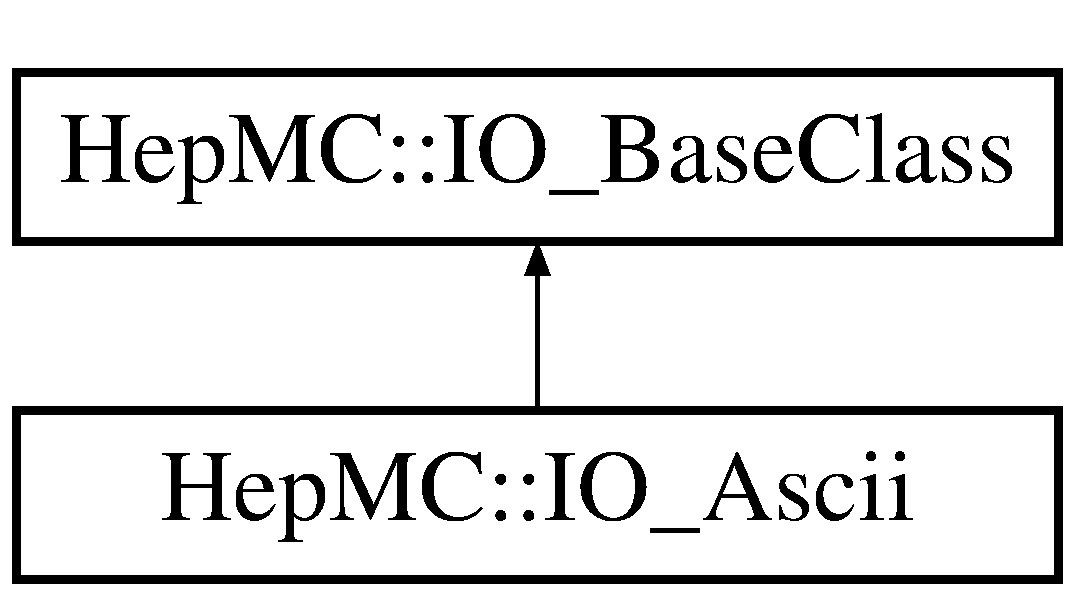
\includegraphics[height=2cm]{classHepMC_1_1IO__Ascii}
\end{center}
\end{figure}
\subsection*{Public Member Functions}
\begin{CompactItemize}
\item 
{\bf IO\_\-Ascii} (const char $\ast$filename=\char`\"{}IO\_\-Ascii.dat\char`\"{}, std::ios::openmode mode=std::ios::out)
\begin{CompactList}\small\item\em constructor requiring a file name and std::ios mode \item\end{CompactList}\item 
virtual {\bf $\sim$IO\_\-Ascii} ()
\item 
void {\bf write\_\-event} (const {\bf Gen\-Event} $\ast$evt)
\begin{CompactList}\small\item\em write this event \item\end{CompactList}\item 
bool {\bf fill\_\-next\_\-event} ({\bf Gen\-Event} $\ast$evt)
\begin{CompactList}\small\item\em get the next event \item\end{CompactList}\item 
void {\bf write\_\-particle\_\-data\_\-table} (const {\bf Particle\-Data\-Table} $\ast$)
\begin{CompactList}\small\item\em write this \doxyref{Particle\-Data\-Table}{p.}{classHepMC_1_1ParticleDataTable} \item\end{CompactList}\item 
bool {\bf fill\_\-particle\_\-data\_\-table} ({\bf Particle\-Data\-Table} $\ast$)
\begin{CompactList}\small\item\em fill this \doxyref{Particle\-Data\-Table}{p.}{classHepMC_1_1ParticleDataTable} \item\end{CompactList}\item 
void {\bf write\_\-comment} (const std::string comment)
\item 
int {\bf rdstate} () const
\begin{CompactList}\small\item\em check the state of the IO stream \item\end{CompactList}\item 
void {\bf clear} ()
\begin{CompactList}\small\item\em clear the IO stream \item\end{CompactList}\item 
void {\bf print} (std::ostream \&ostr=std::cout) const
\begin{CompactList}\small\item\em write to ostr \item\end{CompactList}\end{CompactItemize}
\subsection*{Protected Member Functions}
\begin{CompactItemize}
\item 
void {\bf write\_\-vertex} ({\bf Gen\-Vertex} $\ast$)
\begin{CompactList}\small\item\em write vertex information \item\end{CompactList}\item 
void {\bf write\_\-particle} ({\bf Gen\-Particle} $\ast${\bf p})
\begin{CompactList}\small\item\em write particle information \item\end{CompactList}\item 
void {\bf write\_\-particle\_\-data} (const {\bf Particle\-Data} $\ast$d)
\begin{CompactList}\small\item\em write \doxyref{Particle\-Data\-Table}{p.}{classHepMC_1_1ParticleDataTable} information \item\end{CompactList}\item 
{\bf Gen\-Vertex} $\ast$ {\bf read\_\-vertex} ({\bf Temp\-Particle\-Map} \&particle\_\-to\_\-end\_\-vertex)
\begin{CompactList}\small\item\em read vertex information \item\end{CompactList}\item 
{\bf Gen\-Particle} $\ast$ {\bf read\_\-particle} ({\bf Temp\-Particle\-Map} \&particle\_\-to\_\-end\_\-vertex)
\begin{CompactList}\small\item\em read \doxyref{Gen\-Particle}{p.}{classHepMC_1_1GenParticle} information \item\end{CompactList}\item 
{\bf Particle\-Data} $\ast$ {\bf read\_\-particle\_\-data} ({\bf Particle\-Data\-Table} $\ast$)
\begin{CompactList}\small\item\em read \doxyref{Particle\-Data\-Table}{p.}{classHepMC_1_1ParticleDataTable} information \item\end{CompactList}\item 
bool {\bf write\_\-end\_\-listing} ()
\begin{CompactList}\small\item\em write end tag \item\end{CompactList}\item 
bool {\bf search\_\-for\_\-key\_\-end} (std::istream \&in, const char $\ast$key)
\begin{CompactList}\small\item\em look for line type (key) \item\end{CompactList}\item 
bool {\bf search\_\-for\_\-key\_\-beginning} (std::istream \&in, const char $\ast$key)
\begin{CompactList}\small\item\em not tested and NOT used anywhere! \item\end{CompactList}\item 
bool {\bf eat\_\-key} (std::iostream \&in, const char $\ast$key)
\begin{CompactList}\small\item\em string manipulation accounting \item\end{CompactList}\item 
int {\bf find\_\-in\_\-map} (const std::map$<$ {\bf Gen\-Vertex} $\ast$, int $>$ \&m, {\bf Gen\-Vertex} $\ast${\bf v}) const
\begin{CompactList}\small\item\em find this vertex in the map of vertices \item\end{CompactList}\item 
void {\bf output} (const double \&)
\begin{CompactList}\small\item\em write double \item\end{CompactList}\item 
void {\bf output} (const int \&)
\begin{CompactList}\small\item\em write int \item\end{CompactList}\item 
void {\bf output} (const long int \&)
\begin{CompactList}\small\item\em write long int \item\end{CompactList}\item 
void {\bf output} (const char \&)
\begin{CompactList}\small\item\em write a single character \item\end{CompactList}\end{CompactItemize}


\subsection{Detailed Description}
\doxyref{IO\_\-Ascii}{p.}{classHepMC_1_1IO__Ascii} is used to read or write from an ascii file. 

Strategy for reading or writing events/particle\-Data as machine readable ascii to a file. When instantiating, the mode of file to be created must be specified. \begin{Desc}
\item[Examples: ]\par


{\bf example\_\-Event\-Selection.cc}, {\bf example\_\-My\-Pythia.cc}, {\bf example\_\-My\-Pythia\-Read.cc}, and {\bf example\_\-Using\-Iterators.cc}.\end{Desc}




Definition at line 63 of file IO\_\-Ascii.h.

\subsection{Constructor \& Destructor Documentation}
\index{HepMC::IO_Ascii@{Hep\-MC::IO\_\-Ascii}!IO_Ascii@{IO\_\-Ascii}}
\index{IO_Ascii@{IO\_\-Ascii}!HepMC::IO_Ascii@{Hep\-MC::IO\_\-Ascii}}
\subsubsection{\setlength{\rightskip}{0pt plus 5cm}Hep\-MC::IO\_\-Ascii::IO\_\-Ascii (const char $\ast$ {\em filename} = {\tt \char`\"{}IO\_\-Ascii.dat\char`\"{}}, std::ios::openmode {\em mode} = {\tt std::ios::out})}\label{classHepMC_1_1IO__Ascii_c06b7b426fb17e00d1f89b3a79e8951b}


constructor requiring a file name and std::ios mode 



Definition at line 15 of file IO\_\-Ascii.cc.\index{HepMC::IO_Ascii@{Hep\-MC::IO\_\-Ascii}!~IO_Ascii@{$\sim$IO\_\-Ascii}}
\index{~IO_Ascii@{$\sim$IO\_\-Ascii}!HepMC::IO_Ascii@{Hep\-MC::IO\_\-Ascii}}
\subsubsection{\setlength{\rightskip}{0pt plus 5cm}Hep\-MC::IO\_\-Ascii::$\sim$IO\_\-Ascii ()\hspace{0.3cm}{\tt  [virtual]}}\label{classHepMC_1_1IO__Ascii_9c5dcfd3d7b362b5f70e2d1a1b38a0b5}




Definition at line 34 of file IO\_\-Ascii.cc.

References write\_\-end\_\-listing().

\subsection{Member Function Documentation}
\index{HepMC::IO_Ascii@{Hep\-MC::IO\_\-Ascii}!write_event@{write\_\-event}}
\index{write_event@{write\_\-event}!HepMC::IO_Ascii@{Hep\-MC::IO\_\-Ascii}}
\subsubsection{\setlength{\rightskip}{0pt plus 5cm}void Hep\-MC::IO\_\-Ascii::write\_\-event (const {\bf Gen\-Event} $\ast$ {\em evt})\hspace{0.3cm}{\tt  [virtual]}}\label{classHepMC_1_1IO__Ascii_f4bb1c23202fd371d1fae5be0c8c2669}


write this event 



Writes evt to m\_\-file. It does NOT delete the event after writing. 

Implements {\bf Hep\-MC::IO\_\-Base\-Class} \doxyref{}{p.}{classHepMC_1_1IO__BaseClass_7929dfd8412207c7904f29652810c1f4}.

Definition at line 49 of file IO\_\-Ascii.cc.

References Hep\-MC::Gen\-Event::alpha\-QCD(), Hep\-MC::Gen\-Event::alpha\-QED(), Hep\-MC::Gen\-Vertex::barcode(), Hep\-MC::Weight\-Container::begin(), Hep\-MC::Weight\-Container::end(), Hep\-MC::Gen\-Event::event\_\-number(), Hep\-MC::Gen\-Event::event\_\-scale(), output(), Hep\-MC::Gen\-Event::random\_\-states(), Hep\-MC::Gen\-Event::signal\_\-process\_\-id(), Hep\-MC::Gen\-Event::signal\_\-process\_\-vertex(), Hep\-MC::Weight\-Container::size(), v, Hep\-MC::version\-Name(), Hep\-MC::Gen\-Event::vertices\_\-begin(), Hep\-MC::Gen\-Event::vertices\_\-end(), Hep\-MC::Gen\-Event::vertices\_\-size(), Hep\-MC::Gen\-Event::weights(), and write\_\-vertex().\index{HepMC::IO_Ascii@{Hep\-MC::IO\_\-Ascii}!fill_next_event@{fill\_\-next\_\-event}}
\index{fill_next_event@{fill\_\-next\_\-event}!HepMC::IO_Ascii@{Hep\-MC::IO\_\-Ascii}}
\subsubsection{\setlength{\rightskip}{0pt plus 5cm}bool Hep\-MC::IO\_\-Ascii::fill\_\-next\_\-event ({\bf Gen\-Event} $\ast$ {\em evt})\hspace{0.3cm}{\tt  [virtual]}}\label{classHepMC_1_1IO__Ascii_74a53d19abf22cca4ff0fbf7e29c00e2}


get the next event 



Implements {\bf Hep\-MC::IO\_\-Base\-Class} \doxyref{}{p.}{classHepMC_1_1IO__BaseClass_f1dffb95a44d521af510f6431a30f942}.

Definition at line 98 of file IO\_\-Ascii.cc.

References Hep\-MC::Gen\-Vertex::add\_\-particle\_\-in(), Hep\-MC::Gen\-Event::add\_\-vertex(), Hep\-MC::Gen\-Event::barcode\_\-to\_\-vertex(), eat\_\-key(), Hep\-MC::Temp\-Particle\-Map::end\_\-vertex(), Hep\-MC::Temp\-Particle\-Map::order\_\-begin(), Hep\-MC::Temp\-Particle\-Map::order\_\-end(), p, read\_\-vertex(), search\_\-for\_\-key\_\-end(), Hep\-MC::Gen\-Event::set\_\-event\_\-number(), Hep\-MC::Gen\-Event::set\_\-random\_\-states(), Hep\-MC::Gen\-Event::set\_\-signal\_\-process\_\-id(), Hep\-MC::Gen\-Event::set\_\-signal\_\-process\_\-vertex(), v, and Hep\-MC::Gen\-Event::weights().\index{HepMC::IO_Ascii@{Hep\-MC::IO\_\-Ascii}!write_particle_data_table@{write\_\-particle\_\-data\_\-table}}
\index{write_particle_data_table@{write\_\-particle\_\-data\_\-table}!HepMC::IO_Ascii@{Hep\-MC::IO\_\-Ascii}}
\subsubsection{\setlength{\rightskip}{0pt plus 5cm}void Hep\-MC::IO\_\-Ascii::write\_\-particle\_\-data\_\-table (const {\bf Particle\-Data\-Table} $\ast$)\hspace{0.3cm}{\tt  [virtual]}}\label{classHepMC_1_1IO__Ascii_f0f17b608da225cb97dde7768c4918de}


write this \doxyref{Particle\-Data\-Table}{p.}{classHepMC_1_1ParticleDataTable} 



Implements {\bf Hep\-MC::IO\_\-Base\-Class} \doxyref{}{p.}{classHepMC_1_1IO__BaseClass_1c2fec4084d50bae9ce6b4cbdf133df4}.

Definition at line 219 of file IO\_\-Ascii.cc.

References Hep\-MC::Particle\-Data\-Table::begin(), Hep\-MC::Particle\-Data\-Table::end(), write\_\-end\_\-listing(), and write\_\-particle\_\-data().\index{HepMC::IO_Ascii@{Hep\-MC::IO\_\-Ascii}!fill_particle_data_table@{fill\_\-particle\_\-data\_\-table}}
\index{fill_particle_data_table@{fill\_\-particle\_\-data\_\-table}!HepMC::IO_Ascii@{Hep\-MC::IO\_\-Ascii}}
\subsubsection{\setlength{\rightskip}{0pt plus 5cm}bool Hep\-MC::IO\_\-Ascii::fill\_\-particle\_\-data\_\-table ({\bf Particle\-Data\-Table} $\ast$)\hspace{0.3cm}{\tt  [virtual]}}\label{classHepMC_1_1IO__Ascii_9c78fbbdfaa4f4623f5644205a41b435}


fill this \doxyref{Particle\-Data\-Table}{p.}{classHepMC_1_1ParticleDataTable} 



Implements {\bf Hep\-MC::IO\_\-Base\-Class} \doxyref{}{p.}{classHepMC_1_1IO__BaseClass_094fc72dd621a2283989525497715feb}.

Definition at line 239 of file IO\_\-Ascii.cc.

References eat\_\-key(), read\_\-particle\_\-data(), search\_\-for\_\-key\_\-end(), and Hep\-MC::Particle\-Data\-Table::set\_\-description().\index{HepMC::IO_Ascii@{Hep\-MC::IO\_\-Ascii}!write_comment@{write\_\-comment}}
\index{write_comment@{write\_\-comment}!HepMC::IO_Ascii@{Hep\-MC::IO\_\-Ascii}}
\subsubsection{\setlength{\rightskip}{0pt plus 5cm}void Hep\-MC::IO\_\-Ascii::write\_\-comment (const std::string {\em comment})}\label{classHepMC_1_1IO__Ascii_077001117775cfa9e868cbd7fddcb611}


insert a comment directly into the output file --- normally you only want to do this at the beginning or end of the file. All comments are preceded with \char`\"{}Hep\-MC::IO\_\-Ascii-COMMENT$\backslash$n\char`\"{} 

Definition at line 204 of file IO\_\-Ascii.cc.

References write\_\-end\_\-listing().\index{HepMC::IO_Ascii@{Hep\-MC::IO\_\-Ascii}!rdstate@{rdstate}}
\index{rdstate@{rdstate}!HepMC::IO_Ascii@{Hep\-MC::IO\_\-Ascii}}
\subsubsection{\setlength{\rightskip}{0pt plus 5cm}int Hep\-MC::IO\_\-Ascii::rdstate () const\hspace{0.3cm}{\tt  [inline]}}\label{classHepMC_1_1IO__Ascii_448847137ffd033e5ad5c9b3d868a511}


check the state of the IO stream 



Definition at line 140 of file IO\_\-Ascii.h.

Referenced by main().\index{HepMC::IO_Ascii@{Hep\-MC::IO\_\-Ascii}!clear@{clear}}
\index{clear@{clear}!HepMC::IO_Ascii@{Hep\-MC::IO\_\-Ascii}}
\subsubsection{\setlength{\rightskip}{0pt plus 5cm}void Hep\-MC::IO\_\-Ascii::clear ()\hspace{0.3cm}{\tt  [inline]}}\label{classHepMC_1_1IO__Ascii_0f9f9cba93c96627d633209892e808fd}


clear the IO stream 



Definition at line 141 of file IO\_\-Ascii.h.\index{HepMC::IO_Ascii@{Hep\-MC::IO\_\-Ascii}!print@{print}}
\index{print@{print}!HepMC::IO_Ascii@{Hep\-MC::IO\_\-Ascii}}
\subsubsection{\setlength{\rightskip}{0pt plus 5cm}void Hep\-MC::IO\_\-Ascii::print (std::ostream \& {\em ostr} = {\tt std::cout}) const\hspace{0.3cm}{\tt  [virtual]}}\label{classHepMC_1_1IO__Ascii_e7ac200517f919bbaad102800cb926af}


write to ostr 



Reimplemented from {\bf Hep\-MC::IO\_\-Base\-Class} \doxyref{}{p.}{classHepMC_1_1IO__BaseClass_52a1503f4107fd3d5f4da02feb45751b}.

Definition at line 39 of file IO\_\-Ascii.cc.\index{HepMC::IO_Ascii@{Hep\-MC::IO\_\-Ascii}!write_vertex@{write\_\-vertex}}
\index{write_vertex@{write\_\-vertex}!HepMC::IO_Ascii@{Hep\-MC::IO\_\-Ascii}}
\subsubsection{\setlength{\rightskip}{0pt plus 5cm}void Hep\-MC::IO\_\-Ascii::write\_\-vertex ({\bf Gen\-Vertex} $\ast$)\hspace{0.3cm}{\tt  [protected]}}\label{classHepMC_1_1IO__Ascii_8b45e348d5e61431403808afe643685c}


write vertex information 



Definition at line 287 of file IO\_\-Ascii.cc.

References output(), v, and write\_\-particle().

Referenced by write\_\-event().\index{HepMC::IO_Ascii@{Hep\-MC::IO\_\-Ascii}!write_particle@{write\_\-particle}}
\index{write_particle@{write\_\-particle}!HepMC::IO_Ascii@{Hep\-MC::IO\_\-Ascii}}
\subsubsection{\setlength{\rightskip}{0pt plus 5cm}void Hep\-MC::IO\_\-Ascii::write\_\-particle ({\bf Gen\-Particle} $\ast$ {\em p})\hspace{0.3cm}{\tt  [protected]}}\label{classHepMC_1_1IO__Ascii_5fbe8a87ace699fbea7d46b002e1ee28}


write particle information 



Definition at line 333 of file IO\_\-Ascii.cc.

References output(), and p.

Referenced by write\_\-vertex().\index{HepMC::IO_Ascii@{Hep\-MC::IO\_\-Ascii}!write_particle_data@{write\_\-particle\_\-data}}
\index{write_particle_data@{write\_\-particle\_\-data}!HepMC::IO_Ascii@{Hep\-MC::IO\_\-Ascii}}
\subsubsection{\setlength{\rightskip}{0pt plus 5cm}void Hep\-MC::IO\_\-Ascii::write\_\-particle\_\-data (const {\bf Particle\-Data} $\ast$ {\em d})\hspace{0.3cm}{\tt  [protected]}}\label{classHepMC_1_1IO__Ascii_98b17dfc4c95129f54670bdd34f476ab}


write \doxyref{Particle\-Data\-Table}{p.}{classHepMC_1_1ParticleDataTable} information 



Definition at line 357 of file IO\_\-Ascii.cc.

References Hep\-MC::Particle\-Data::charge(), Hep\-MC::Particle\-Data::clifetime(), Hep\-MC::Particle\-Data::mass(), Hep\-MC::Particle\-Data::name(), output(), Hep\-MC::Particle\-Data::pdg\_\-id(), and Hep\-MC::Particle\-Data::spin().

Referenced by write\_\-particle\_\-data\_\-table().\index{HepMC::IO_Ascii@{Hep\-MC::IO\_\-Ascii}!read_vertex@{read\_\-vertex}}
\index{read_vertex@{read\_\-vertex}!HepMC::IO_Ascii@{Hep\-MC::IO\_\-Ascii}}
\subsubsection{\setlength{\rightskip}{0pt plus 5cm}{\bf Gen\-Vertex} $\ast$ Hep\-MC::IO\_\-Ascii::read\_\-vertex ({\bf Temp\-Particle\-Map} \& {\em particle\_\-to\_\-end\_\-vertex})\hspace{0.3cm}{\tt  [protected]}}\label{classHepMC_1_1IO__Ascii_28326aa1b8ac4719f953187a5292e74e}


read vertex information 



Definition at line 376 of file IO\_\-Ascii.cc.

References read\_\-particle(), and v.

Referenced by fill\_\-next\_\-event().\index{HepMC::IO_Ascii@{Hep\-MC::IO\_\-Ascii}!read_particle@{read\_\-particle}}
\index{read_particle@{read\_\-particle}!HepMC::IO_Ascii@{Hep\-MC::IO\_\-Ascii}}
\subsubsection{\setlength{\rightskip}{0pt plus 5cm}{\bf Gen\-Particle} $\ast$ Hep\-MC::IO\_\-Ascii::read\_\-particle ({\bf Temp\-Particle\-Map} \& {\em particle\_\-to\_\-end\_\-vertex})\hspace{0.3cm}{\tt  [protected]}}\label{classHepMC_1_1IO__Ascii_46cbdffba08e6b671efeeb8d2a59ceee}


read \doxyref{Gen\-Particle}{p.}{classHepMC_1_1GenParticle} information 



Definition at line 412 of file IO\_\-Ascii.cc.

References Hep\-MC::Temp\-Particle\-Map::add\-End\-Particle(), p, and Hep\-MC::Flow::set\_\-icode().

Referenced by read\_\-vertex().\index{HepMC::IO_Ascii@{Hep\-MC::IO\_\-Ascii}!read_particle_data@{read\_\-particle\_\-data}}
\index{read_particle_data@{read\_\-particle\_\-data}!HepMC::IO_Ascii@{Hep\-MC::IO\_\-Ascii}}
\subsubsection{\setlength{\rightskip}{0pt plus 5cm}{\bf Particle\-Data} $\ast$ Hep\-MC::IO\_\-Ascii::read\_\-particle\_\-data ({\bf Particle\-Data\-Table} $\ast$)\hspace{0.3cm}{\tt  [protected]}}\label{classHepMC_1_1IO__Ascii_9532e3a57853993e657d2041f4328e5a}


read \doxyref{Particle\-Data\-Table}{p.}{classHepMC_1_1ParticleDataTable} information 



Definition at line 453 of file IO\_\-Ascii.cc.

References Hep\-MC::Particle\-Data\-Table::insert().

Referenced by fill\_\-particle\_\-data\_\-table().\index{HepMC::IO_Ascii@{Hep\-MC::IO\_\-Ascii}!write_end_listing@{write\_\-end\_\-listing}}
\index{write_end_listing@{write\_\-end\_\-listing}!HepMC::IO_Ascii@{Hep\-MC::IO\_\-Ascii}}
\subsubsection{\setlength{\rightskip}{0pt plus 5cm}bool Hep\-MC::IO\_\-Ascii::write\_\-end\_\-listing ()\hspace{0.3cm}{\tt  [protected]}}\label{classHepMC_1_1IO__Ascii_964b5e58c07bee41daeb1f75a149b741}


write end tag 



Definition at line 475 of file IO\_\-Ascii.cc.

Referenced by write\_\-comment(), write\_\-particle\_\-data\_\-table(), and $\sim$IO\_\-Ascii().\index{HepMC::IO_Ascii@{Hep\-MC::IO\_\-Ascii}!search_for_key_end@{search\_\-for\_\-key\_\-end}}
\index{search_for_key_end@{search\_\-for\_\-key\_\-end}!HepMC::IO_Ascii@{Hep\-MC::IO\_\-Ascii}}
\subsubsection{\setlength{\rightskip}{0pt plus 5cm}bool Hep\-MC::IO\_\-Ascii::search\_\-for\_\-key\_\-end (std::istream \& {\em in}, const char $\ast$ {\em key})\hspace{0.3cm}{\tt  [protected]}}\label{classHepMC_1_1IO__Ascii_20e1758a4a9c2c58948a7132bb24742e}


look for line type (key) 



reads characters from in until the string of characters matching key is found (success) or EOF is reached (failure). It stops immediately thereafter. Returns T/F for success/fail 

Definition at line 484 of file IO\_\-Ascii.cc.

Referenced by fill\_\-next\_\-event(), fill\_\-particle\_\-data\_\-table(), and search\_\-for\_\-key\_\-beginning().\index{HepMC::IO_Ascii@{Hep\-MC::IO\_\-Ascii}!search_for_key_beginning@{search\_\-for\_\-key\_\-beginning}}
\index{search_for_key_beginning@{search\_\-for\_\-key\_\-beginning}!HepMC::IO_Ascii@{Hep\-MC::IO\_\-Ascii}}
\subsubsection{\setlength{\rightskip}{0pt plus 5cm}bool Hep\-MC::IO\_\-Ascii::search\_\-for\_\-key\_\-beginning (std::istream \& {\em in}, const char $\ast$ {\em key})\hspace{0.3cm}{\tt  [protected]}}\label{classHepMC_1_1IO__Ascii_3a4c5f95251702a9de28457cbdb3f31c}


not tested and NOT used anywhere! 



not tested and NOT used anywhere! 

Definition at line 500 of file IO\_\-Ascii.cc.

References search\_\-for\_\-key\_\-end().\index{HepMC::IO_Ascii@{Hep\-MC::IO\_\-Ascii}!eat_key@{eat\_\-key}}
\index{eat_key@{eat\_\-key}!HepMC::IO_Ascii@{Hep\-MC::IO\_\-Ascii}}
\subsubsection{\setlength{\rightskip}{0pt plus 5cm}bool Hep\-MC::IO\_\-Ascii::eat\_\-key (std::iostream \& {\em in}, const char $\ast$ {\em key})\hspace{0.3cm}{\tt  [protected]}}\label{classHepMC_1_1IO__Ascii_678152917165ed16050e678b9a4c0ace}


string manipulation accounting 



eats the character string key from istream in - only if the key is the very next occurence in the stream if the key is not the next occurence, it eats nothing ... i.e. it puts back whatever it would have eaten. 

Definition at line 514 of file IO\_\-Ascii.cc.

Referenced by fill\_\-next\_\-event(), and fill\_\-particle\_\-data\_\-table().\index{HepMC::IO_Ascii@{Hep\-MC::IO\_\-Ascii}!find_in_map@{find\_\-in\_\-map}}
\index{find_in_map@{find\_\-in\_\-map}!HepMC::IO_Ascii@{Hep\-MC::IO\_\-Ascii}}
\subsubsection{\setlength{\rightskip}{0pt plus 5cm}int Hep\-MC::IO\_\-Ascii::find\_\-in\_\-map (const std::map$<$ {\bf Gen\-Vertex} $\ast$, int $>$ \& {\em m}, {\bf Gen\-Vertex} $\ast$ {\em v}) const\hspace{0.3cm}{\tt  [protected]}}\label{classHepMC_1_1IO__Ascii_a95041c6d8f52e4dce4f3dd9d78ae1cf}


find this vertex in the map of vertices 



Definition at line 543 of file IO\_\-Ascii.cc.

References v.\index{HepMC::IO_Ascii@{Hep\-MC::IO\_\-Ascii}!output@{output}}
\index{output@{output}!HepMC::IO_Ascii@{Hep\-MC::IO\_\-Ascii}}
\subsubsection{\setlength{\rightskip}{0pt plus 5cm}void Hep\-MC::IO\_\-Ascii::output (const double \&)\hspace{0.3cm}{\tt  [inline, protected]}}\label{classHepMC_1_1IO__Ascii_0fdbb0f0a472f9654b0f658689fe324b}


write double 



Definition at line 130 of file IO\_\-Ascii.h.

Referenced by write\_\-event(), write\_\-particle(), write\_\-particle\_\-data(), and write\_\-vertex().\index{HepMC::IO_Ascii@{Hep\-MC::IO\_\-Ascii}!output@{output}}
\index{output@{output}!HepMC::IO_Ascii@{Hep\-MC::IO\_\-Ascii}}
\subsubsection{\setlength{\rightskip}{0pt plus 5cm}void Hep\-MC::IO\_\-Ascii::output (const int \&)\hspace{0.3cm}{\tt  [inline, protected]}}\label{classHepMC_1_1IO__Ascii_91aef2c96813e8f6210ec447f3caf881}


write int 



Definition at line 137 of file IO\_\-Ascii.h.\index{HepMC::IO_Ascii@{Hep\-MC::IO\_\-Ascii}!output@{output}}
\index{output@{output}!HepMC::IO_Ascii@{Hep\-MC::IO\_\-Ascii}}
\subsubsection{\setlength{\rightskip}{0pt plus 5cm}void Hep\-MC::IO\_\-Ascii::output (const long int \&)\hspace{0.3cm}{\tt  [inline, protected]}}\label{classHepMC_1_1IO__Ascii_b9a7019104c61b13fc0eae238ee402c7}


write long int 



Definition at line 138 of file IO\_\-Ascii.h.\index{HepMC::IO_Ascii@{Hep\-MC::IO\_\-Ascii}!output@{output}}
\index{output@{output}!HepMC::IO_Ascii@{Hep\-MC::IO\_\-Ascii}}
\subsubsection{\setlength{\rightskip}{0pt plus 5cm}void Hep\-MC::IO\_\-Ascii::output (const char \&)\hspace{0.3cm}{\tt  [inline, protected]}}\label{classHepMC_1_1IO__Ascii_fc6e08fc832eeb23e77a02fe949bea98}


write a single character 



Definition at line 139 of file IO\_\-Ascii.h.

The documentation for this class was generated from the following files:\begin{CompactItemize}
\item 
{\bf IO\_\-Ascii.h}\item 
{\bf IO\_\-Ascii.cc}\end{CompactItemize}

\section{Hep\-MC::IO\_\-Ascii\-Particles Class Reference}
\label{classHepMC_1_1IO__AsciiParticles}\index{HepMC::IO_AsciiParticles@{HepMC::IO\_\-AsciiParticles}}
event input/output in ascii format for eye and machine reading  


{\tt \#include $<$IO\_\-Ascii\-Particles.h$>$}

Inheritance diagram for Hep\-MC::IO\_\-Ascii\-Particles::\begin{figure}[H]
\begin{center}
\leavevmode
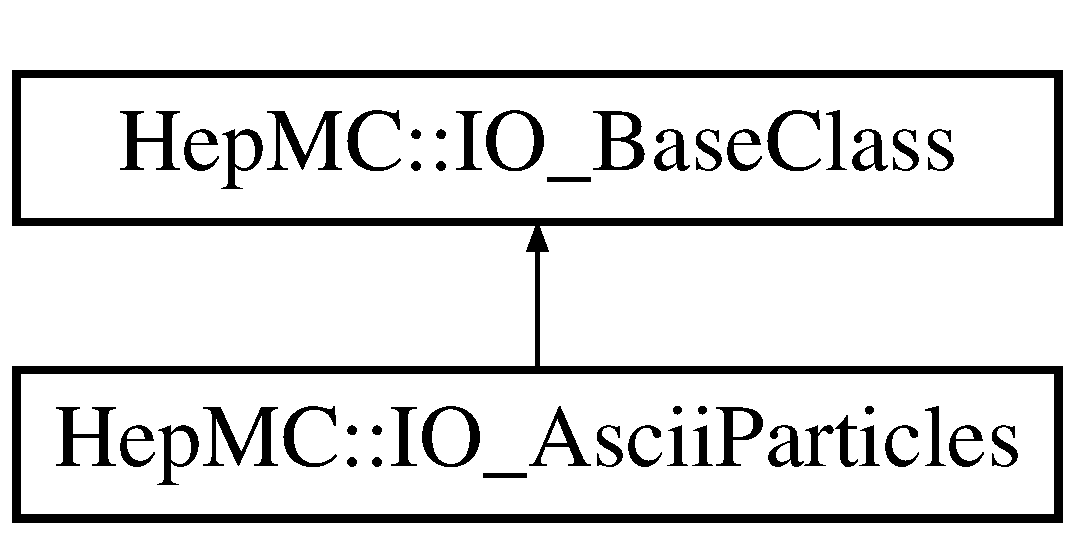
\includegraphics[height=2cm]{classHepMC_1_1IO__AsciiParticles}
\end{center}
\end{figure}
\subsection*{Public Member Functions}
\begin{CompactItemize}
\item 
{\bf IO\_\-Ascii\-Particles} (const char $\ast$filename=\char`\"{}IO\_\-Ascii\-Particles.dat\char`\"{}, std::ios::openmode mode=std::ios::out)
\begin{CompactList}\small\item\em constructor requiring a file name and std::ios mode \item\end{CompactList}\item 
virtual {\bf $\sim$IO\_\-Ascii\-Particles} ()
\item 
void {\bf write\_\-event} (const {\bf Gen\-Event} $\ast$evt)
\begin{CompactList}\small\item\em write this event \item\end{CompactList}\item 
bool {\bf fill\_\-next\_\-event} ({\bf Gen\-Event} $\ast$evt)
\begin{CompactList}\small\item\em get the next event \item\end{CompactList}\item 
void {\bf write\_\-particle\_\-data\_\-table} (const {\bf Particle\-Data\-Table} $\ast$)
\begin{CompactList}\small\item\em write this \doxyref{Particle\-Data\-Table}{p.}{classHepMC_1_1ParticleDataTable} \item\end{CompactList}\item 
bool {\bf fill\_\-particle\_\-data\_\-table} ({\bf Particle\-Data\-Table} $\ast$)
\begin{CompactList}\small\item\em fill this \doxyref{Particle\-Data\-Table}{p.}{classHepMC_1_1ParticleDataTable} \item\end{CompactList}\item 
void {\bf write\_\-comment} (const std::string comment)
\item 
void {\bf set\-Precision} (int iprec)
\begin{CompactList}\small\item\em set output precision \item\end{CompactList}\item 
int {\bf rdstate} () const
\begin{CompactList}\small\item\em check the state of the IO stream \item\end{CompactList}\item 
void {\bf clear} ()
\begin{CompactList}\small\item\em clear the IO stream \item\end{CompactList}\item 
void {\bf print} (std::ostream \&ostr=std::cout) const
\begin{CompactList}\small\item\em write to ostr \item\end{CompactList}\end{CompactItemize}
\subsection*{Protected Member Functions}
\begin{CompactItemize}
\item 
bool {\bf write\_\-end\_\-listing} ()
\begin{CompactList}\small\item\em write end tag \item\end{CompactList}\end{CompactItemize}


\subsection{Detailed Description}
event input/output in ascii format for eye and machine reading 

Strategy for reading or writing events/particle\-Data as machine readable ascii to a file. When instantiating, the mode of file to be created must be specified. \begin{Desc}
\item[Examples: ]\par


{\bf example\_\-Pythia\-Particle.cc}.\end{Desc}




Definition at line 54 of file IO\_\-Ascii\-Particles.h.

\subsection{Constructor \& Destructor Documentation}
\index{HepMC::IO_AsciiParticles@{Hep\-MC::IO\_\-Ascii\-Particles}!IO_AsciiParticles@{IO\_\-AsciiParticles}}
\index{IO_AsciiParticles@{IO\_\-AsciiParticles}!HepMC::IO_AsciiParticles@{Hep\-MC::IO\_\-Ascii\-Particles}}
\subsubsection{\setlength{\rightskip}{0pt plus 5cm}Hep\-MC::IO\_\-Ascii\-Particles::IO\_\-Ascii\-Particles (const char $\ast$ {\em filename} = {\tt \char`\"{}IO\_\-AsciiParticles.dat\char`\"{}}, std::ios::openmode {\em mode} = {\tt std::ios::out})}\label{classHepMC_1_1IO__AsciiParticles_79fa989e218044213efef5c874d6d5de}


constructor requiring a file name and std::ios mode 



Definition at line 18 of file IO\_\-Ascii\-Particles.cc.\index{HepMC::IO_AsciiParticles@{Hep\-MC::IO\_\-Ascii\-Particles}!~IO_AsciiParticles@{$\sim$IO\_\-AsciiParticles}}
\index{~IO_AsciiParticles@{$\sim$IO\_\-AsciiParticles}!HepMC::IO_AsciiParticles@{Hep\-MC::IO\_\-Ascii\-Particles}}
\subsubsection{\setlength{\rightskip}{0pt plus 5cm}Hep\-MC::IO\_\-Ascii\-Particles::$\sim$IO\_\-Ascii\-Particles ()\hspace{0.3cm}{\tt  [virtual]}}\label{classHepMC_1_1IO__AsciiParticles_7dc3782a4ca5f516149488a55f3605d7}




Definition at line 47 of file IO\_\-Ascii\-Particles.cc.

\subsection{Member Function Documentation}
\index{HepMC::IO_AsciiParticles@{Hep\-MC::IO\_\-Ascii\-Particles}!write_event@{write\_\-event}}
\index{write_event@{write\_\-event}!HepMC::IO_AsciiParticles@{Hep\-MC::IO\_\-Ascii\-Particles}}
\subsubsection{\setlength{\rightskip}{0pt plus 5cm}void Hep\-MC::IO\_\-Ascii\-Particles::write\_\-event (const {\bf Gen\-Event} $\ast$ {\em evt})\hspace{0.3cm}{\tt  [virtual]}}\label{classHepMC_1_1IO__AsciiParticles_2d45b9474967ec0cdeccece86d5d8c5e}


write this event 



Implements {\bf Hep\-MC::IO\_\-Base\-Class} \doxyref{}{p.}{classHepMC_1_1IO__BaseClass_7929dfd8412207c7904f29652810c1f4}.

Definition at line 64 of file IO\_\-Ascii\-Particles.cc.

References Hep\-MC::Gen\-Event::alpha\-QCD(), Hep\-MC::Gen\-Event::alpha\-QED(), Hep\-MC::Gen\-Vertex::barcode(), Hep\-MC::Weight\-Container::begin(), Hep\-MC::Weight\-Container::end(), Hep\-MC::Gen\-Event::event\_\-number(), Hep\-MC::Gen\-Event::event\_\-scale(), Hep\-MC::Gen\-Event::particles\_\-begin(), Hep\-MC::Gen\-Event::particles\_\-end(), Hep\-MC::Gen\-Event::particles\_\-size(), Hep\-MC::Gen\-Event::random\_\-states(), Hep\-MC::Gen\-Event::signal\_\-process\_\-id(), Hep\-MC::Gen\-Event::signal\_\-process\_\-vertex(), Hep\-MC::Weight\-Container::size(), Hep\-MC::version\-Name(), Hep\-MC::Gen\-Event::vertices\_\-size(), and Hep\-MC::Gen\-Event::weights().\index{HepMC::IO_AsciiParticles@{Hep\-MC::IO\_\-Ascii\-Particles}!fill_next_event@{fill\_\-next\_\-event}}
\index{fill_next_event@{fill\_\-next\_\-event}!HepMC::IO_AsciiParticles@{Hep\-MC::IO\_\-Ascii\-Particles}}
\subsubsection{\setlength{\rightskip}{0pt plus 5cm}bool Hep\-MC::IO\_\-Ascii\-Particles::fill\_\-next\_\-event ({\bf Gen\-Event} $\ast$ {\em evt})\hspace{0.3cm}{\tt  [virtual]}}\label{classHepMC_1_1IO__AsciiParticles_fdd859891c2ac09f8758d081357c17ce}


get the next event 



Implements {\bf Hep\-MC::IO\_\-Base\-Class} \doxyref{}{p.}{classHepMC_1_1IO__BaseClass_f1dffb95a44d521af510f6431a30f942}.

Definition at line 180 of file IO\_\-Ascii\-Particles.cc.\index{HepMC::IO_AsciiParticles@{Hep\-MC::IO\_\-Ascii\-Particles}!write_particle_data_table@{write\_\-particle\_\-data\_\-table}}
\index{write_particle_data_table@{write\_\-particle\_\-data\_\-table}!HepMC::IO_AsciiParticles@{Hep\-MC::IO\_\-Ascii\-Particles}}
\subsubsection{\setlength{\rightskip}{0pt plus 5cm}void Hep\-MC::IO\_\-Ascii\-Particles::write\_\-particle\_\-data\_\-table (const {\bf Particle\-Data\-Table} $\ast$)\hspace{0.3cm}{\tt  [inline, virtual]}}\label{classHepMC_1_1IO__AsciiParticles_94c2db38f83b52f5724777d17399457c}


write this \doxyref{Particle\-Data\-Table}{p.}{classHepMC_1_1ParticleDataTable} 



Implements {\bf Hep\-MC::IO\_\-Base\-Class} \doxyref{}{p.}{classHepMC_1_1IO__BaseClass_1c2fec4084d50bae9ce6b4cbdf133df4}.

Definition at line 106 of file IO\_\-Ascii\-Particles.h.\index{HepMC::IO_AsciiParticles@{Hep\-MC::IO\_\-Ascii\-Particles}!fill_particle_data_table@{fill\_\-particle\_\-data\_\-table}}
\index{fill_particle_data_table@{fill\_\-particle\_\-data\_\-table}!HepMC::IO_AsciiParticles@{Hep\-MC::IO\_\-Ascii\-Particles}}
\subsubsection{\setlength{\rightskip}{0pt plus 5cm}bool Hep\-MC::IO\_\-Ascii\-Particles::fill\_\-particle\_\-data\_\-table ({\bf Particle\-Data\-Table} $\ast$)\hspace{0.3cm}{\tt  [inline, virtual]}}\label{classHepMC_1_1IO__AsciiParticles_e03b03bffb39bced419dc2c1a4de0b1d}


fill this \doxyref{Particle\-Data\-Table}{p.}{classHepMC_1_1ParticleDataTable} 



Implements {\bf Hep\-MC::IO\_\-Base\-Class} \doxyref{}{p.}{classHepMC_1_1IO__BaseClass_094fc72dd621a2283989525497715feb}.

Definition at line 107 of file IO\_\-Ascii\-Particles.h.\index{HepMC::IO_AsciiParticles@{Hep\-MC::IO\_\-Ascii\-Particles}!write_comment@{write\_\-comment}}
\index{write_comment@{write\_\-comment}!HepMC::IO_AsciiParticles@{Hep\-MC::IO\_\-Ascii\-Particles}}
\subsubsection{\setlength{\rightskip}{0pt plus 5cm}void Hep\-MC::IO\_\-Ascii\-Particles::write\_\-comment (const std::string {\em comment})}\label{classHepMC_1_1IO__AsciiParticles_c835b3026984b78fba4ac8380d483672}


insert a comment directly into the output file --- normally you only want to do this at the beginning or end of the file. All comments are preceded with \char`\"{}Hep\-MC::IO\_\-Ascii\-Particles-COMMENT$\backslash$n\char`\"{} 

Definition at line 203 of file IO\_\-Ascii\-Particles.cc.

References write\_\-end\_\-listing().\index{HepMC::IO_AsciiParticles@{Hep\-MC::IO\_\-Ascii\-Particles}!setPrecision@{setPrecision}}
\index{setPrecision@{setPrecision}!HepMC::IO_AsciiParticles@{Hep\-MC::IO\_\-Ascii\-Particles}}
\subsubsection{\setlength{\rightskip}{0pt plus 5cm}void Hep\-MC::IO\_\-Ascii\-Particles::set\-Precision (int {\em iprec})\hspace{0.3cm}{\tt  [inline]}}\label{classHepMC_1_1IO__AsciiParticles_2534fb6f39e0bb6db30dd16675f11cd1}


set output precision 



Definition at line 100 of file IO\_\-Ascii\-Particles.h.\index{HepMC::IO_AsciiParticles@{Hep\-MC::IO\_\-Ascii\-Particles}!rdstate@{rdstate}}
\index{rdstate@{rdstate}!HepMC::IO_AsciiParticles@{Hep\-MC::IO\_\-Ascii\-Particles}}
\subsubsection{\setlength{\rightskip}{0pt plus 5cm}int Hep\-MC::IO\_\-Ascii\-Particles::rdstate () const\hspace{0.3cm}{\tt  [inline]}}\label{classHepMC_1_1IO__AsciiParticles_783f27d815fc7c52fcdcf8aa4a75d4eb}


check the state of the IO stream 



Definition at line 98 of file IO\_\-Ascii\-Particles.h.\index{HepMC::IO_AsciiParticles@{Hep\-MC::IO\_\-Ascii\-Particles}!clear@{clear}}
\index{clear@{clear}!HepMC::IO_AsciiParticles@{Hep\-MC::IO\_\-Ascii\-Particles}}
\subsubsection{\setlength{\rightskip}{0pt plus 5cm}void Hep\-MC::IO\_\-Ascii\-Particles::clear ()\hspace{0.3cm}{\tt  [inline]}}\label{classHepMC_1_1IO__AsciiParticles_6cf4f71c3306f8d070b723629f416b57}


clear the IO stream 



Definition at line 99 of file IO\_\-Ascii\-Particles.h.\index{HepMC::IO_AsciiParticles@{Hep\-MC::IO\_\-Ascii\-Particles}!print@{print}}
\index{print@{print}!HepMC::IO_AsciiParticles@{Hep\-MC::IO\_\-Ascii\-Particles}}
\subsubsection{\setlength{\rightskip}{0pt plus 5cm}void Hep\-MC::IO\_\-Ascii\-Particles::print (std::ostream \& {\em ostr} = {\tt std::cout}) const\hspace{0.3cm}{\tt  [virtual]}}\label{classHepMC_1_1IO__AsciiParticles_0007e73c1637d4af793b475862719095}


write to ostr 



Reimplemented from {\bf Hep\-MC::IO\_\-Base\-Class} \doxyref{}{p.}{classHepMC_1_1IO__BaseClass_52a1503f4107fd3d5f4da02feb45751b}.

Definition at line 54 of file IO\_\-Ascii\-Particles.cc.\index{HepMC::IO_AsciiParticles@{Hep\-MC::IO\_\-Ascii\-Particles}!write_end_listing@{write\_\-end\_\-listing}}
\index{write_end_listing@{write\_\-end\_\-listing}!HepMC::IO_AsciiParticles@{Hep\-MC::IO\_\-Ascii\-Particles}}
\subsubsection{\setlength{\rightskip}{0pt plus 5cm}bool Hep\-MC::IO\_\-Ascii\-Particles::write\_\-end\_\-listing ()\hspace{0.3cm}{\tt  [protected]}}\label{classHepMC_1_1IO__AsciiParticles_691d927301d269af979892d757239d1c}


write end tag 



Definition at line 218 of file IO\_\-Ascii\-Particles.cc.

Referenced by write\_\-comment().

The documentation for this class was generated from the following files:\begin{CompactItemize}
\item 
{\bf IO\_\-Ascii\-Particles.h}\item 
{\bf IO\_\-Ascii\-Particles.cc}\end{CompactItemize}

\section{Hep\-MC::IO\_\-Base\-Class Class Reference}
\label{classHepMC_1_1IO__BaseClass}\index{HepMC::IO_BaseClass@{HepMC::IO\_\-BaseClass}}
all input/output classes inherit from \doxyref{IO\_\-Base\-Class}{p.}{classHepMC_1_1IO__BaseClass}  


{\tt \#include $<$IO\_\-Base\-Class.h$>$}

Inheritance diagram for Hep\-MC::IO\_\-Base\-Class::\begin{figure}[H]
\begin{center}
\leavevmode
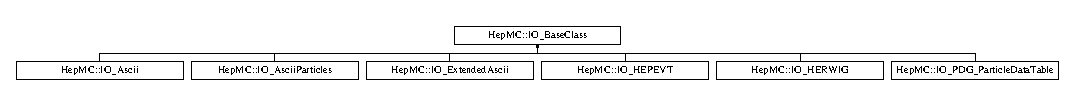
\includegraphics[height=0.840841cm]{classHepMC_1_1IO__BaseClass}
\end{center}
\end{figure}
\subsection*{Public Member Functions}
\begin{CompactItemize}
\item 
virtual {\bf $\sim$IO\_\-Base\-Class} ()
\item 
virtual void {\bf write\_\-event} (const {\bf Gen\-Event} $\ast$)=0
\begin{CompactList}\small\item\em write this \doxyref{Gen\-Event}{p.}{classHepMC_1_1GenEvent} \item\end{CompactList}\item 
virtual bool {\bf fill\_\-next\_\-event} ({\bf Gen\-Event} $\ast$)=0
\begin{CompactList}\small\item\em fill this \doxyref{Gen\-Event}{p.}{classHepMC_1_1GenEvent} \item\end{CompactList}\item 
virtual void {\bf write\_\-particle\_\-data\_\-table} (const {\bf Particle\-Data\-Table} $\ast$)=0
\begin{CompactList}\small\item\em write this \doxyref{Particle\-Data\-Table}{p.}{classHepMC_1_1ParticleDataTable} \item\end{CompactList}\item 
virtual bool {\bf fill\_\-particle\_\-data\_\-table} ({\bf Particle\-Data\-Table} $\ast$)=0
\begin{CompactList}\small\item\em fill this \doxyref{Particle\-Data\-Table}{p.}{classHepMC_1_1ParticleDataTable} \item\end{CompactList}\item 
virtual void {\bf print} (std::ostream \&ostr=std::cout) const
\begin{CompactList}\small\item\em write output to ostr \item\end{CompactList}\item 
{\bf Gen\-Event} $\ast$ {\bf read\_\-next\_\-event} ()
\begin{CompactList}\small\item\em do not over-ride \item\end{CompactList}\item 
{\bf Particle\-Data\-Table} $\ast$ {\bf read\_\-particle\_\-data\_\-table} ()
\begin{CompactList}\small\item\em do not over-ride \item\end{CompactList}\item 
virtual {\bf Gen\-Event} $\ast$\& {\bf operator$>$$>$} ({\bf Gen\-Event} $\ast$\&)
\begin{CompactList}\small\item\em the same as read\_\-next\_\-event \item\end{CompactList}\item 
virtual const {\bf Gen\-Event} $\ast$\& {\bf operator$<$$<$} (const {\bf Gen\-Event} $\ast$\&)
\begin{CompactList}\small\item\em the same as write\_\-event \item\end{CompactList}\item 
virtual {\bf Gen\-Event} $\ast$\& {\bf operator$<$$<$} ({\bf Gen\-Event} $\ast$\&)
\begin{CompactList}\small\item\em the same as write\_\-event \item\end{CompactList}\item 
virtual {\bf Particle\-Data\-Table} $\ast$\& {\bf operator$>$$>$} ({\bf Particle\-Data\-Table} $\ast$\&)
\begin{CompactList}\small\item\em the same as read\_\-particle\_\-data\_\-table \item\end{CompactList}\item 
virtual const {\bf Particle\-Data\-Table} $\ast$\& {\bf operator$<$$<$} (const {\bf Particle\-Data\-Table} $\ast$\&)
\begin{CompactList}\small\item\em the same as write\_\-particle\_\-data\_\-table \item\end{CompactList}\item 
virtual {\bf Particle\-Data\-Table} $\ast$\& {\bf operator$<$$<$} ({\bf Particle\-Data\-Table} $\ast$\&)
\begin{CompactList}\small\item\em the same as write\_\-particle\_\-data\_\-table \item\end{CompactList}\end{CompactItemize}


\subsection{Detailed Description}
all input/output classes inherit from \doxyref{IO\_\-Base\-Class}{p.}{classHepMC_1_1IO__BaseClass} 

If you want to write a new IO class, then inherit from this class and re-define read\_\-event() and \doxyref{write\_\-event()}{p.}{classHepMC_1_1IO__BaseClass_7929dfd8412207c7904f29652810c1f4} 



Definition at line 35 of file IO\_\-Base\-Class.h.

\subsection{Constructor \& Destructor Documentation}
\index{HepMC::IO_BaseClass@{Hep\-MC::IO\_\-Base\-Class}!~IO_BaseClass@{$\sim$IO\_\-BaseClass}}
\index{~IO_BaseClass@{$\sim$IO\_\-BaseClass}!HepMC::IO_BaseClass@{Hep\-MC::IO\_\-Base\-Class}}
\subsubsection{\setlength{\rightskip}{0pt plus 5cm}virtual Hep\-MC::IO\_\-Base\-Class::$\sim$IO\_\-Base\-Class ()\hspace{0.3cm}{\tt  [inline, virtual]}}\label{classHepMC_1_1IO__BaseClass_b5a73e9efa32ec30ae67d546657699fd}




Definition at line 37 of file IO\_\-Base\-Class.h.

\subsection{Member Function Documentation}
\index{HepMC::IO_BaseClass@{Hep\-MC::IO\_\-Base\-Class}!write_event@{write\_\-event}}
\index{write_event@{write\_\-event}!HepMC::IO_BaseClass@{Hep\-MC::IO\_\-Base\-Class}}
\subsubsection{\setlength{\rightskip}{0pt plus 5cm}virtual void Hep\-MC::IO\_\-Base\-Class::write\_\-event (const {\bf Gen\-Event} $\ast$)\hspace{0.3cm}{\tt  [pure virtual]}}\label{classHepMC_1_1IO__BaseClass_7929dfd8412207c7904f29652810c1f4}


write this \doxyref{Gen\-Event}{p.}{classHepMC_1_1GenEvent} 



Implemented in {\bf Hep\-MC::IO\_\-Ascii} \doxyref{}{p.}{classHepMC_1_1IO__Ascii_f4bb1c23202fd371d1fae5be0c8c2669}, {\bf Hep\-MC::IO\_\-Ascii\-Particles} \doxyref{}{p.}{classHepMC_1_1IO__AsciiParticles_2d45b9474967ec0cdeccece86d5d8c5e}, {\bf Hep\-MC::IO\_\-Extended\-Ascii} \doxyref{}{p.}{classHepMC_1_1IO__ExtendedAscii_a7c87ec189b071358e2dd5062a69e817}, and {\bf Hep\-MC::IO\_\-HEPEVT} \doxyref{}{p.}{classHepMC_1_1IO__HEPEVT_adbd36a8914a4cc275be26856884da43}.

Referenced by operator$<$$<$().\index{HepMC::IO_BaseClass@{Hep\-MC::IO\_\-Base\-Class}!fill_next_event@{fill\_\-next\_\-event}}
\index{fill_next_event@{fill\_\-next\_\-event}!HepMC::IO_BaseClass@{Hep\-MC::IO\_\-Base\-Class}}
\subsubsection{\setlength{\rightskip}{0pt plus 5cm}virtual bool Hep\-MC::IO\_\-Base\-Class::fill\_\-next\_\-event ({\bf Gen\-Event} $\ast$)\hspace{0.3cm}{\tt  [pure virtual]}}\label{classHepMC_1_1IO__BaseClass_f1dffb95a44d521af510f6431a30f942}


fill this \doxyref{Gen\-Event}{p.}{classHepMC_1_1GenEvent} 



Implemented in {\bf Hep\-MC::IO\_\-Ascii} \doxyref{}{p.}{classHepMC_1_1IO__Ascii_74a53d19abf22cca4ff0fbf7e29c00e2}, {\bf Hep\-MC::IO\_\-Ascii\-Particles} \doxyref{}{p.}{classHepMC_1_1IO__AsciiParticles_fdd859891c2ac09f8758d081357c17ce}, {\bf Hep\-MC::IO\_\-Extended\-Ascii} \doxyref{}{p.}{classHepMC_1_1IO__ExtendedAscii_ce48dffeff50b3bd7ee6df679f421690}, {\bf Hep\-MC::IO\_\-HEPEVT} \doxyref{}{p.}{classHepMC_1_1IO__HEPEVT_e4bcb5527c18d161c11edd19bad49416}, and {\bf Hep\-MC::IO\_\-HERWIG} \doxyref{}{p.}{classHepMC_1_1IO__HERWIG_7a49968897062f0e977053bcdf176e17}.

Referenced by read\_\-next\_\-event().\index{HepMC::IO_BaseClass@{Hep\-MC::IO\_\-Base\-Class}!write_particle_data_table@{write\_\-particle\_\-data\_\-table}}
\index{write_particle_data_table@{write\_\-particle\_\-data\_\-table}!HepMC::IO_BaseClass@{Hep\-MC::IO\_\-Base\-Class}}
\subsubsection{\setlength{\rightskip}{0pt plus 5cm}virtual void Hep\-MC::IO\_\-Base\-Class::write\_\-particle\_\-data\_\-table (const {\bf Particle\-Data\-Table} $\ast$)\hspace{0.3cm}{\tt  [pure virtual]}}\label{classHepMC_1_1IO__BaseClass_1c2fec4084d50bae9ce6b4cbdf133df4}


write this \doxyref{Particle\-Data\-Table}{p.}{classHepMC_1_1ParticleDataTable} 



Implemented in {\bf Hep\-MC::IO\_\-Ascii} \doxyref{}{p.}{classHepMC_1_1IO__Ascii_f0f17b608da225cb97dde7768c4918de}, {\bf Hep\-MC::IO\_\-Ascii\-Particles} \doxyref{}{p.}{classHepMC_1_1IO__AsciiParticles_94c2db38f83b52f5724777d17399457c}, and {\bf Hep\-MC::IO\_\-Extended\-Ascii} \doxyref{}{p.}{classHepMC_1_1IO__ExtendedAscii_483444f704444961d6b5317770c9a411}.

Referenced by operator$<$$<$().\index{HepMC::IO_BaseClass@{Hep\-MC::IO\_\-Base\-Class}!fill_particle_data_table@{fill\_\-particle\_\-data\_\-table}}
\index{fill_particle_data_table@{fill\_\-particle\_\-data\_\-table}!HepMC::IO_BaseClass@{Hep\-MC::IO\_\-Base\-Class}}
\subsubsection{\setlength{\rightskip}{0pt plus 5cm}virtual bool Hep\-MC::IO\_\-Base\-Class::fill\_\-particle\_\-data\_\-table ({\bf Particle\-Data\-Table} $\ast$)\hspace{0.3cm}{\tt  [pure virtual]}}\label{classHepMC_1_1IO__BaseClass_094fc72dd621a2283989525497715feb}


fill this \doxyref{Particle\-Data\-Table}{p.}{classHepMC_1_1ParticleDataTable} 



Implemented in {\bf Hep\-MC::IO\_\-Ascii} \doxyref{}{p.}{classHepMC_1_1IO__Ascii_9c78fbbdfaa4f4623f5644205a41b435}, {\bf Hep\-MC::IO\_\-Ascii\-Particles} \doxyref{}{p.}{classHepMC_1_1IO__AsciiParticles_e03b03bffb39bced419dc2c1a4de0b1d}, {\bf Hep\-MC::IO\_\-Extended\-Ascii} \doxyref{}{p.}{classHepMC_1_1IO__ExtendedAscii_113228dd5201c5f8c71e59a7df2c4c0e}, and {\bf Hep\-MC::IO\_\-PDG\_\-Particle\-Data\-Table} \doxyref{}{p.}{classHepMC_1_1IO__PDG__ParticleDataTable_6f0aee31fa762dfe83a686e4925adede}.

Referenced by read\_\-particle\_\-data\_\-table().\index{HepMC::IO_BaseClass@{Hep\-MC::IO\_\-Base\-Class}!print@{print}}
\index{print@{print}!HepMC::IO_BaseClass@{Hep\-MC::IO\_\-Base\-Class}}
\subsubsection{\setlength{\rightskip}{0pt plus 5cm}void Hep\-MC::IO\_\-Base\-Class::print (std::ostream \& {\em ostr} = {\tt std::cout}) const\hspace{0.3cm}{\tt  [inline, virtual]}}\label{classHepMC_1_1IO__BaseClass_52a1503f4107fd3d5f4da02feb45751b}


write output to ostr 



Reimplemented in {\bf Hep\-MC::IO\_\-Ascii} \doxyref{}{p.}{classHepMC_1_1IO__Ascii_e7ac200517f919bbaad102800cb926af}, {\bf Hep\-MC::IO\_\-Ascii\-Particles} \doxyref{}{p.}{classHepMC_1_1IO__AsciiParticles_0007e73c1637d4af793b475862719095}, {\bf Hep\-MC::IO\_\-Extended\-Ascii} \doxyref{}{p.}{classHepMC_1_1IO__ExtendedAscii_f4dcc1b894210117034a591024d9575e}, {\bf Hep\-MC::IO\_\-HEPEVT} \doxyref{}{p.}{classHepMC_1_1IO__HEPEVT_5f360aa251e909cc77f1a9f9d45d7abf}, {\bf Hep\-MC::IO\_\-HERWIG} \doxyref{}{p.}{classHepMC_1_1IO__HERWIG_ab6853a2888f6e2f628039b9079fe120}, and {\bf Hep\-MC::IO\_\-PDG\_\-Particle\-Data\-Table} \doxyref{}{p.}{classHepMC_1_1IO__PDG__ParticleDataTable_3d125861cb0d1cafe6550e125111ff72}.

Definition at line 117 of file IO\_\-Base\-Class.h.\index{HepMC::IO_BaseClass@{Hep\-MC::IO\_\-Base\-Class}!read_next_event@{read\_\-next\_\-event}}
\index{read_next_event@{read\_\-next\_\-event}!HepMC::IO_BaseClass@{Hep\-MC::IO\_\-Base\-Class}}
\subsubsection{\setlength{\rightskip}{0pt plus 5cm}{\bf Gen\-Event} $\ast$ Hep\-MC::IO\_\-Base\-Class::read\_\-next\_\-event ()\hspace{0.3cm}{\tt  [inline]}}\label{classHepMC_1_1IO__BaseClass_d6f5d122a998c9c33e80379a18e0708f}


do not over-ride 



creates a new event and fills it by calling the sister method read\_\-next\_\-event( Gen\-Event$\ast$ ) \begin{Desc}
\item[Examples: ]\par
{\bf example\_\-My\-Herwig.cc}, {\bf example\_\-My\-Pythia.cc}, {\bf example\_\-My\-Pythia\-Only\-To\-Hep\-MC.cc}, {\bf example\_\-My\-Pythia\-Read.cc}, {\bf example\_\-My\-Pythia\-With\-Event\-Selection.cc}, and {\bf example\_\-Pythia\-Particle.cc}.\end{Desc}


Definition at line 87 of file IO\_\-Base\-Class.h.

References fill\_\-next\_\-event().

Referenced by main(), and operator$>$$>$().\index{HepMC::IO_BaseClass@{Hep\-MC::IO\_\-Base\-Class}!read_particle_data_table@{read\_\-particle\_\-data\_\-table}}
\index{read_particle_data_table@{read\_\-particle\_\-data\_\-table}!HepMC::IO_BaseClass@{Hep\-MC::IO\_\-Base\-Class}}
\subsubsection{\setlength{\rightskip}{0pt plus 5cm}{\bf Particle\-Data\-Table} $\ast$ Hep\-MC::IO\_\-Base\-Class::read\_\-particle\_\-data\_\-table ()\hspace{0.3cm}{\tt  [inline]}}\label{classHepMC_1_1IO__BaseClass_585b6d798bfa5b4e47fc6447c503aad6}


do not over-ride 



creates a new particle data table and fills it by calling the sister method read\_\-particle\_\-data\_\-table( Particle\-Data\-Table$\ast$ ) 

Definition at line 103 of file IO\_\-Base\-Class.h.

References fill\_\-particle\_\-data\_\-table().

Referenced by main(), and operator$>$$>$().\index{HepMC::IO_BaseClass@{Hep\-MC::IO\_\-Base\-Class}!operator>>@{operator$>$$>$}}
\index{operator>>@{operator$>$$>$}!HepMC::IO_BaseClass@{Hep\-MC::IO\_\-Base\-Class}}
\subsubsection{\setlength{\rightskip}{0pt plus 5cm}{\bf Gen\-Event} $\ast$\& Hep\-MC::IO\_\-Base\-Class::operator$>$$>$ ({\bf Gen\-Event} $\ast$\&)\hspace{0.3cm}{\tt  [inline, virtual]}}\label{classHepMC_1_1IO__BaseClass_c92cd53e61d6363bd21a0b9dc2b6f6d0}


the same as read\_\-next\_\-event 



Definition at line 121 of file IO\_\-Base\-Class.h.

References read\_\-next\_\-event().\index{HepMC::IO_BaseClass@{Hep\-MC::IO\_\-Base\-Class}!operator<<@{operator$<$$<$}}
\index{operator<<@{operator$<$$<$}!HepMC::IO_BaseClass@{Hep\-MC::IO\_\-Base\-Class}}
\subsubsection{\setlength{\rightskip}{0pt plus 5cm}const {\bf Gen\-Event} $\ast$\& Hep\-MC::IO\_\-Base\-Class::operator$<$$<$ (const {\bf Gen\-Event} $\ast$\&)\hspace{0.3cm}{\tt  [inline, virtual]}}\label{classHepMC_1_1IO__BaseClass_9b3a17aaa907a330ad622166ac8cb63e}


the same as write\_\-event 



Definition at line 126 of file IO\_\-Base\-Class.h.

References write\_\-event().\index{HepMC::IO_BaseClass@{Hep\-MC::IO\_\-Base\-Class}!operator<<@{operator$<$$<$}}
\index{operator<<@{operator$<$$<$}!HepMC::IO_BaseClass@{Hep\-MC::IO\_\-Base\-Class}}
\subsubsection{\setlength{\rightskip}{0pt plus 5cm}{\bf Gen\-Event} $\ast$\& Hep\-MC::IO\_\-Base\-Class::operator$<$$<$ ({\bf Gen\-Event} $\ast$\&)\hspace{0.3cm}{\tt  [inline, virtual]}}\label{classHepMC_1_1IO__BaseClass_eb332f776b74cf45eb35472ded4c89d6}


the same as write\_\-event 



Definition at line 132 of file IO\_\-Base\-Class.h.

References write\_\-event().\index{HepMC::IO_BaseClass@{Hep\-MC::IO\_\-Base\-Class}!operator>>@{operator$>$$>$}}
\index{operator>>@{operator$>$$>$}!HepMC::IO_BaseClass@{Hep\-MC::IO\_\-Base\-Class}}
\subsubsection{\setlength{\rightskip}{0pt plus 5cm}{\bf Particle\-Data\-Table} $\ast$\& Hep\-MC::IO\_\-Base\-Class::operator$>$$>$ ({\bf Particle\-Data\-Table} $\ast$\&)\hspace{0.3cm}{\tt  [inline, virtual]}}\label{classHepMC_1_1IO__BaseClass_7677efde67e39363a298a1c05f0db488}


the same as read\_\-particle\_\-data\_\-table 



Definition at line 137 of file IO\_\-Base\-Class.h.

References read\_\-particle\_\-data\_\-table().\index{HepMC::IO_BaseClass@{Hep\-MC::IO\_\-Base\-Class}!operator<<@{operator$<$$<$}}
\index{operator<<@{operator$<$$<$}!HepMC::IO_BaseClass@{Hep\-MC::IO\_\-Base\-Class}}
\subsubsection{\setlength{\rightskip}{0pt plus 5cm}const {\bf Particle\-Data\-Table} $\ast$\& Hep\-MC::IO\_\-Base\-Class::operator$<$$<$ (const {\bf Particle\-Data\-Table} $\ast$\&)\hspace{0.3cm}{\tt  [inline, virtual]}}\label{classHepMC_1_1IO__BaseClass_601f34e218c0938e8d41f6094c6cf9d1}


the same as write\_\-particle\_\-data\_\-table 



Definition at line 143 of file IO\_\-Base\-Class.h.

References write\_\-particle\_\-data\_\-table().\index{HepMC::IO_BaseClass@{Hep\-MC::IO\_\-Base\-Class}!operator<<@{operator$<$$<$}}
\index{operator<<@{operator$<$$<$}!HepMC::IO_BaseClass@{Hep\-MC::IO\_\-Base\-Class}}
\subsubsection{\setlength{\rightskip}{0pt plus 5cm}{\bf Particle\-Data\-Table} $\ast$\& Hep\-MC::IO\_\-Base\-Class::operator$<$$<$ ({\bf Particle\-Data\-Table} $\ast$\&)\hspace{0.3cm}{\tt  [inline, virtual]}}\label{classHepMC_1_1IO__BaseClass_ef0b6c14cbb4ba488811963f74d613d3}


the same as write\_\-particle\_\-data\_\-table 



Definition at line 149 of file IO\_\-Base\-Class.h.

References write\_\-particle\_\-data\_\-table().

The documentation for this class was generated from the following file:\begin{CompactItemize}
\item 
{\bf IO\_\-Base\-Class.h}\end{CompactItemize}

\section{Hep\-MC::IO\_\-Extended\-Ascii Class Reference}
\label{classHepMC_1_1IO__ExtendedAscii}\index{HepMC::IO_ExtendedAscii@{HepMC::IO\_\-ExtendedAscii}}
\doxyref{IO\_\-Extended\-Ascii}{p.}{classHepMC_1_1IO__ExtendedAscii} also deals with \doxyref{Heavy\-Ion}{p.}{classHepMC_1_1HeavyIon} and \doxyref{Pdf\-Info}{p.}{classHepMC_1_1PdfInfo}.  


{\tt \#include $<$IO\_\-Extended\-Ascii.h$>$}

Inheritance diagram for Hep\-MC::IO\_\-Extended\-Ascii::\begin{figure}[H]
\begin{center}
\leavevmode
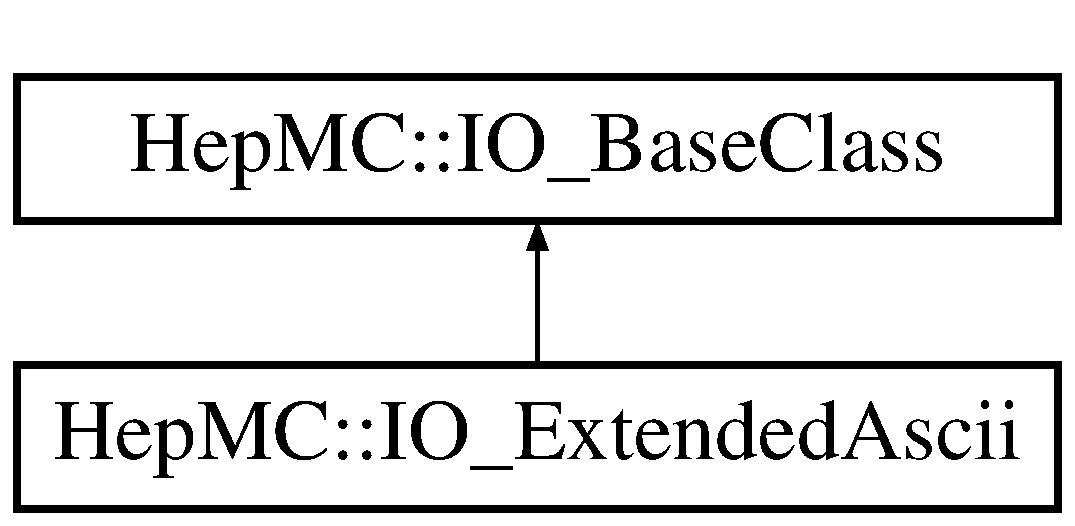
\includegraphics[height=2cm]{classHepMC_1_1IO__ExtendedAscii}
\end{center}
\end{figure}
\subsection*{Public Member Functions}
\begin{CompactItemize}
\item 
{\bf IO\_\-Extended\-Ascii} (const char $\ast$filename=\char`\"{}IO\_\-Extended\-Ascii.dat\char`\"{}, std::ios::openmode mode=std::ios::out)
\begin{CompactList}\small\item\em constructor requiring a file name and std::ios mode \item\end{CompactList}\item 
virtual {\bf $\sim$IO\_\-Extended\-Ascii} ()
\item 
void {\bf write\_\-event} (const {\bf Gen\-Event} $\ast$evt)
\begin{CompactList}\small\item\em write this event \item\end{CompactList}\item 
bool {\bf fill\_\-next\_\-event} ({\bf Gen\-Event} $\ast$evt)
\begin{CompactList}\small\item\em get the next event \item\end{CompactList}\item 
void {\bf write\_\-particle\_\-data\_\-table} (const {\bf Particle\-Data\-Table} $\ast$)
\begin{CompactList}\small\item\em write this \doxyref{Particle\-Data\-Table}{p.}{classHepMC_1_1ParticleDataTable} \item\end{CompactList}\item 
bool {\bf fill\_\-particle\_\-data\_\-table} ({\bf Particle\-Data\-Table} $\ast$)
\begin{CompactList}\small\item\em fill this \doxyref{Particle\-Data\-Table}{p.}{classHepMC_1_1ParticleDataTable} \item\end{CompactList}\item 
void {\bf write\_\-comment} (const std::string comment)
\item 
int {\bf rdstate} () const
\begin{CompactList}\small\item\em check the state of the IO stream \item\end{CompactList}\item 
void {\bf clear} ()
\begin{CompactList}\small\item\em clear the IO stream \item\end{CompactList}\item 
void {\bf print} (std::ostream \&ostr=std::cout) const
\begin{CompactList}\small\item\em write to ostr \item\end{CompactList}\end{CompactItemize}
\subsection*{Protected Member Functions}
\begin{CompactItemize}
\item 
void {\bf write\_\-vertex} ({\bf Gen\-Vertex} $\ast$)
\begin{CompactList}\small\item\em write vertex information \item\end{CompactList}\item 
void {\bf write\_\-beam\_\-particles} (std::pair$<$ {\bf Hep\-MC::Gen\-Particle} $\ast$, {\bf Hep\-MC::Gen\-Particle} $\ast$ $>$)
\begin{CompactList}\small\item\em write beam particle information \item\end{CompactList}\item 
void {\bf write\_\-heavy\_\-ion} ({\bf Heavy\-Ion} $\ast$)
\begin{CompactList}\small\item\em write heavy ion information \item\end{CompactList}\item 
void {\bf write\_\-pdf\_\-info} ({\bf Pdf\-Info} $\ast$)
\begin{CompactList}\small\item\em write PDF information \item\end{CompactList}\item 
void {\bf write\_\-particle} ({\bf Gen\-Particle} $\ast${\bf p})
\begin{CompactList}\small\item\em write particle information \item\end{CompactList}\item 
void {\bf write\_\-particle\_\-data} (const {\bf Particle\-Data} $\ast$d)
\begin{CompactList}\small\item\em write particle data information \item\end{CompactList}\item 
{\bf Gen\-Vertex} $\ast$ {\bf read\_\-vertex} ({\bf Temp\-Particle\-Map} \&particle\_\-to\_\-end\_\-vertex)
\begin{CompactList}\small\item\em read vertex information \item\end{CompactList}\item 
{\bf Gen\-Particle} $\ast$ {\bf read\_\-particle} ({\bf Temp\-Particle\-Map} \&particle\_\-to\_\-end\_\-vertex)
\begin{CompactList}\small\item\em read \doxyref{Gen\-Particle}{p.}{classHepMC_1_1GenParticle} information \item\end{CompactList}\item 
{\bf Particle\-Data} $\ast$ {\bf read\_\-particle\_\-data} ({\bf Particle\-Data\-Table} $\ast$)
\begin{CompactList}\small\item\em read particle data table information \item\end{CompactList}\item 
{\bf Heavy\-Ion} $\ast$ {\bf read\_\-heavy\_\-ion} ()
\begin{CompactList}\small\item\em read heavy ion information \item\end{CompactList}\item 
{\bf Pdf\-Info} $\ast$ {\bf read\_\-pdf\_\-info} ()
\begin{CompactList}\small\item\em read PDF information \item\end{CompactList}\item 
bool {\bf write\_\-end\_\-listing} ()
\begin{CompactList}\small\item\em write end tag \item\end{CompactList}\item 
bool {\bf search\_\-for\_\-key\_\-end} (std::istream \&in, const char $\ast$key)
\begin{CompactList}\small\item\em look for line type (key) \item\end{CompactList}\item 
bool {\bf search\_\-for\_\-key\_\-beginning} (std::istream \&in, const char $\ast$key)
\begin{CompactList}\small\item\em look for line type (key) \item\end{CompactList}\item 
bool {\bf eat\_\-key} (std::iostream \&in, const char $\ast$key)
\begin{CompactList}\small\item\em string manipulation accounting \item\end{CompactList}\item 
int {\bf find\_\-in\_\-map} (const std::map$<$ {\bf Hep\-MC::Gen\-Vertex} $\ast$, int $>$ \&m, {\bf Gen\-Vertex} $\ast${\bf v}) const
\begin{CompactList}\small\item\em find this vertex in the map of vertices \item\end{CompactList}\item 
void {\bf output} (const double \&)
\begin{CompactList}\small\item\em write double \item\end{CompactList}\item 
void {\bf output} (const float \&)
\begin{CompactList}\small\item\em write float \item\end{CompactList}\item 
void {\bf output} (const int \&)
\begin{CompactList}\small\item\em write int \item\end{CompactList}\item 
void {\bf output} (const long int \&)
\begin{CompactList}\small\item\em write long int \item\end{CompactList}\item 
void {\bf output} (const char \&)
\begin{CompactList}\small\item\em write a single character \item\end{CompactList}\end{CompactItemize}


\subsection{Detailed Description}
\doxyref{IO\_\-Extended\-Ascii}{p.}{classHepMC_1_1IO__ExtendedAscii} also deals with \doxyref{Heavy\-Ion}{p.}{classHepMC_1_1HeavyIon} and \doxyref{Pdf\-Info}{p.}{classHepMC_1_1PdfInfo}. 

event input/output in ascii format for machine reading extended format contains \doxyref{Heavy\-Ion}{p.}{classHepMC_1_1HeavyIon} and \doxyref{Pdf\-Info}{p.}{classHepMC_1_1PdfInfo} classes \begin{Desc}
\item[Examples: ]\par


{\bf example\_\-My\-Pythia.cc}.\end{Desc}




Definition at line 64 of file IO\_\-Extended\-Ascii.h.

\subsection{Constructor \& Destructor Documentation}
\index{HepMC::IO_ExtendedAscii@{Hep\-MC::IO\_\-Extended\-Ascii}!IO_ExtendedAscii@{IO\_\-ExtendedAscii}}
\index{IO_ExtendedAscii@{IO\_\-ExtendedAscii}!HepMC::IO_ExtendedAscii@{Hep\-MC::IO\_\-Extended\-Ascii}}
\subsubsection{\setlength{\rightskip}{0pt plus 5cm}Hep\-MC::IO\_\-Extended\-Ascii::IO\_\-Extended\-Ascii (const char $\ast$ {\em filename} = {\tt \char`\"{}IO\_\-ExtendedAscii.dat\char`\"{}}, std::ios::openmode {\em mode} = {\tt std::ios::out})}\label{classHepMC_1_1IO__ExtendedAscii_7ccca1e73789ef8b5d727f241fe50ac9}


constructor requiring a file name and std::ios mode 



Definition at line 18 of file IO\_\-Extended\-Ascii.cc.\index{HepMC::IO_ExtendedAscii@{Hep\-MC::IO\_\-Extended\-Ascii}!~IO_ExtendedAscii@{$\sim$IO\_\-ExtendedAscii}}
\index{~IO_ExtendedAscii@{$\sim$IO\_\-ExtendedAscii}!HepMC::IO_ExtendedAscii@{Hep\-MC::IO\_\-Extended\-Ascii}}
\subsubsection{\setlength{\rightskip}{0pt plus 5cm}Hep\-MC::IO\_\-Extended\-Ascii::$\sim$IO\_\-Extended\-Ascii ()\hspace{0.3cm}{\tt  [virtual]}}\label{classHepMC_1_1IO__ExtendedAscii_cdfe51865c7cb3af761934e3c0824467}




Definition at line 37 of file IO\_\-Extended\-Ascii.cc.

References write\_\-end\_\-listing().

\subsection{Member Function Documentation}
\index{HepMC::IO_ExtendedAscii@{Hep\-MC::IO\_\-Extended\-Ascii}!write_event@{write\_\-event}}
\index{write_event@{write\_\-event}!HepMC::IO_ExtendedAscii@{Hep\-MC::IO\_\-Extended\-Ascii}}
\subsubsection{\setlength{\rightskip}{0pt plus 5cm}void Hep\-MC::IO\_\-Extended\-Ascii::write\_\-event (const {\bf Gen\-Event} $\ast$ {\em evt})\hspace{0.3cm}{\tt  [virtual]}}\label{classHepMC_1_1IO__ExtendedAscii_a7c87ec189b071358e2dd5062a69e817}


write this event 



Writes evt to m\_\-file. It does NOT delete the event after writing. 

Implements {\bf Hep\-MC::IO\_\-Base\-Class} \doxyref{}{p.}{classHepMC_1_1IO__BaseClass_7929dfd8412207c7904f29652810c1f4}.

Definition at line 52 of file IO\_\-Extended\-Ascii.cc.

References Hep\-MC::Gen\-Event::alpha\-QCD(), Hep\-MC::Gen\-Event::alpha\-QED(), Hep\-MC::Gen\-Vertex::barcode(), Hep\-MC::Gen\-Event::beam\_\-particles(), Hep\-MC::Weight\-Container::begin(), Hep\-MC::Weight\-Container::end(), Hep\-MC::Gen\-Event::event\_\-number(), Hep\-MC::Gen\-Event::event\_\-scale(), Hep\-MC::Gen\-Event::heavy\_\-ion(), Hep\-MC::Gen\-Event::mpi(), output(), Hep\-MC::Gen\-Event::pdf\_\-info(), Hep\-MC::Gen\-Event::random\_\-states(), Hep\-MC::Gen\-Event::signal\_\-process\_\-id(), Hep\-MC::Gen\-Event::signal\_\-process\_\-vertex(), Hep\-MC::Weight\-Container::size(), v, Hep\-MC::version\-Name(), Hep\-MC::Gen\-Event::vertices\_\-begin(), Hep\-MC::Gen\-Event::vertices\_\-end(), Hep\-MC::Gen\-Event::vertices\_\-size(), Hep\-MC::Gen\-Event::weights(), write\_\-beam\_\-particles(), write\_\-heavy\_\-ion(), write\_\-pdf\_\-info(), and write\_\-vertex().\index{HepMC::IO_ExtendedAscii@{Hep\-MC::IO\_\-Extended\-Ascii}!fill_next_event@{fill\_\-next\_\-event}}
\index{fill_next_event@{fill\_\-next\_\-event}!HepMC::IO_ExtendedAscii@{Hep\-MC::IO\_\-Extended\-Ascii}}
\subsubsection{\setlength{\rightskip}{0pt plus 5cm}bool Hep\-MC::IO\_\-Extended\-Ascii::fill\_\-next\_\-event ({\bf Gen\-Event} $\ast$ {\em evt})\hspace{0.3cm}{\tt  [virtual]}}\label{classHepMC_1_1IO__ExtendedAscii_ce48dffeff50b3bd7ee6df679f421690}


get the next event 



Implements {\bf Hep\-MC::IO\_\-Base\-Class} \doxyref{}{p.}{classHepMC_1_1IO__BaseClass_f1dffb95a44d521af510f6431a30f942}.

Definition at line 105 of file IO\_\-Extended\-Ascii.cc.

References Hep\-MC::Gen\-Vertex::add\_\-particle\_\-in(), Hep\-MC::Gen\-Event::add\_\-vertex(), Hep\-MC::Gen\-Event::barcode\_\-to\_\-vertex(), eat\_\-key(), Hep\-MC::Temp\-Particle\-Map::end\_\-vertex(), Hep\-MC::Temp\-Particle\-Map::order\_\-begin(), Hep\-MC::Temp\-Particle\-Map::order\_\-end(), p, read\_\-heavy\_\-ion(), read\_\-pdf\_\-info(), read\_\-vertex(), search\_\-for\_\-key\_\-end(), Hep\-MC::Gen\-Event::set\_\-beam\_\-particles(), Hep\-MC::Gen\-Event::set\_\-event\_\-number(), Hep\-MC::Gen\-Event::set\_\-heavy\_\-ion(), Hep\-MC::Gen\-Event::set\_\-mpi(), Hep\-MC::Gen\-Event::set\_\-pdf\_\-info(), Hep\-MC::Gen\-Event::set\_\-random\_\-states(), Hep\-MC::Gen\-Event::set\_\-signal\_\-process\_\-id(), Hep\-MC::Gen\-Event::set\_\-signal\_\-process\_\-vertex(), v, and Hep\-MC::Gen\-Event::weights().\index{HepMC::IO_ExtendedAscii@{Hep\-MC::IO\_\-Extended\-Ascii}!write_particle_data_table@{write\_\-particle\_\-data\_\-table}}
\index{write_particle_data_table@{write\_\-particle\_\-data\_\-table}!HepMC::IO_ExtendedAscii@{Hep\-MC::IO\_\-Extended\-Ascii}}
\subsubsection{\setlength{\rightskip}{0pt plus 5cm}void Hep\-MC::IO\_\-Extended\-Ascii::write\_\-particle\_\-data\_\-table (const {\bf Particle\-Data\-Table} $\ast$)\hspace{0.3cm}{\tt  [virtual]}}\label{classHepMC_1_1IO__ExtendedAscii_483444f704444961d6b5317770c9a411}


write this \doxyref{Particle\-Data\-Table}{p.}{classHepMC_1_1ParticleDataTable} 



Implements {\bf Hep\-MC::IO\_\-Base\-Class} \doxyref{}{p.}{classHepMC_1_1IO__BaseClass_1c2fec4084d50bae9ce6b4cbdf133df4}.

Definition at line 239 of file IO\_\-Extended\-Ascii.cc.

References Hep\-MC::Particle\-Data\-Table::begin(), Hep\-MC::Particle\-Data\-Table::end(), write\_\-end\_\-listing(), and write\_\-particle\_\-data().\index{HepMC::IO_ExtendedAscii@{Hep\-MC::IO\_\-Extended\-Ascii}!fill_particle_data_table@{fill\_\-particle\_\-data\_\-table}}
\index{fill_particle_data_table@{fill\_\-particle\_\-data\_\-table}!HepMC::IO_ExtendedAscii@{Hep\-MC::IO\_\-Extended\-Ascii}}
\subsubsection{\setlength{\rightskip}{0pt plus 5cm}bool Hep\-MC::IO\_\-Extended\-Ascii::fill\_\-particle\_\-data\_\-table ({\bf Particle\-Data\-Table} $\ast$)\hspace{0.3cm}{\tt  [virtual]}}\label{classHepMC_1_1IO__ExtendedAscii_113228dd5201c5f8c71e59a7df2c4c0e}


fill this \doxyref{Particle\-Data\-Table}{p.}{classHepMC_1_1ParticleDataTable} 



Implements {\bf Hep\-MC::IO\_\-Base\-Class} \doxyref{}{p.}{classHepMC_1_1IO__BaseClass_094fc72dd621a2283989525497715feb}.

Definition at line 259 of file IO\_\-Extended\-Ascii.cc.

References eat\_\-key(), read\_\-particle\_\-data(), search\_\-for\_\-key\_\-end(), and Hep\-MC::Particle\-Data\-Table::set\_\-description().\index{HepMC::IO_ExtendedAscii@{Hep\-MC::IO\_\-Extended\-Ascii}!write_comment@{write\_\-comment}}
\index{write_comment@{write\_\-comment}!HepMC::IO_ExtendedAscii@{Hep\-MC::IO\_\-Extended\-Ascii}}
\subsubsection{\setlength{\rightskip}{0pt plus 5cm}void Hep\-MC::IO\_\-Extended\-Ascii::write\_\-comment (const std::string {\em comment})}\label{classHepMC_1_1IO__ExtendedAscii_ebf7128bf373d3f514828af999064c67}


insert a comment directly into the output file --- normally you only want to do this at the beginning or end of the file. All comments are preceded with \char`\"{}Hep\-MC::IO\_\-Extended\-Ascii-COMMENT$\backslash$n\char`\"{} 

Definition at line 224 of file IO\_\-Extended\-Ascii.cc.

References write\_\-end\_\-listing().\index{HepMC::IO_ExtendedAscii@{Hep\-MC::IO\_\-Extended\-Ascii}!rdstate@{rdstate}}
\index{rdstate@{rdstate}!HepMC::IO_ExtendedAscii@{Hep\-MC::IO\_\-Extended\-Ascii}}
\subsubsection{\setlength{\rightskip}{0pt plus 5cm}int Hep\-MC::IO\_\-Extended\-Ascii::rdstate () const\hspace{0.3cm}{\tt  [inline]}}\label{classHepMC_1_1IO__ExtendedAscii_9cbf4c13083ef03c22edc04229c90b89}


check the state of the IO stream 



Definition at line 159 of file IO\_\-Extended\-Ascii.h.\index{HepMC::IO_ExtendedAscii@{Hep\-MC::IO\_\-Extended\-Ascii}!clear@{clear}}
\index{clear@{clear}!HepMC::IO_ExtendedAscii@{Hep\-MC::IO\_\-Extended\-Ascii}}
\subsubsection{\setlength{\rightskip}{0pt plus 5cm}void Hep\-MC::IO\_\-Extended\-Ascii::clear ()\hspace{0.3cm}{\tt  [inline]}}\label{classHepMC_1_1IO__ExtendedAscii_d2ca3ee00c2a58cf7ed6407d7c412fb0}


clear the IO stream 



Definition at line 160 of file IO\_\-Extended\-Ascii.h.\index{HepMC::IO_ExtendedAscii@{Hep\-MC::IO\_\-Extended\-Ascii}!print@{print}}
\index{print@{print}!HepMC::IO_ExtendedAscii@{Hep\-MC::IO\_\-Extended\-Ascii}}
\subsubsection{\setlength{\rightskip}{0pt plus 5cm}void Hep\-MC::IO\_\-Extended\-Ascii::print (std::ostream \& {\em ostr} = {\tt std::cout}) const\hspace{0.3cm}{\tt  [virtual]}}\label{classHepMC_1_1IO__ExtendedAscii_f4dcc1b894210117034a591024d9575e}


write to ostr 



Reimplemented from {\bf Hep\-MC::IO\_\-Base\-Class} \doxyref{}{p.}{classHepMC_1_1IO__BaseClass_52a1503f4107fd3d5f4da02feb45751b}.

Definition at line 42 of file IO\_\-Extended\-Ascii.cc.\index{HepMC::IO_ExtendedAscii@{Hep\-MC::IO\_\-Extended\-Ascii}!write_vertex@{write\_\-vertex}}
\index{write_vertex@{write\_\-vertex}!HepMC::IO_ExtendedAscii@{Hep\-MC::IO\_\-Extended\-Ascii}}
\subsubsection{\setlength{\rightskip}{0pt plus 5cm}void Hep\-MC::IO\_\-Extended\-Ascii::write\_\-vertex ({\bf Gen\-Vertex} $\ast$)\hspace{0.3cm}{\tt  [protected]}}\label{classHepMC_1_1IO__ExtendedAscii_d36702b408a97b1ebeffe0442bf73464}


write vertex information 



Definition at line 307 of file IO\_\-Extended\-Ascii.cc.

References output(), v, and write\_\-particle().

Referenced by write\_\-event().\index{HepMC::IO_ExtendedAscii@{Hep\-MC::IO\_\-Extended\-Ascii}!write_beam_particles@{write\_\-beam\_\-particles}}
\index{write_beam_particles@{write\_\-beam\_\-particles}!HepMC::IO_ExtendedAscii@{Hep\-MC::IO\_\-Extended\-Ascii}}
\subsubsection{\setlength{\rightskip}{0pt plus 5cm}void Hep\-MC::IO\_\-Extended\-Ascii::write\_\-beam\_\-particles (std::pair$<$ {\bf Hep\-MC::Gen\-Particle} $\ast$, {\bf Hep\-MC::Gen\-Particle} $\ast$ $>$)\hspace{0.3cm}{\tt  [protected]}}\label{classHepMC_1_1IO__ExtendedAscii_7c48c3aa56e9f6a9559d0af46fc90161}


write beam particle information 



Referenced by write\_\-event().\index{HepMC::IO_ExtendedAscii@{Hep\-MC::IO\_\-Extended\-Ascii}!write_heavy_ion@{write\_\-heavy\_\-ion}}
\index{write_heavy_ion@{write\_\-heavy\_\-ion}!HepMC::IO_ExtendedAscii@{Hep\-MC::IO\_\-Extended\-Ascii}}
\subsubsection{\setlength{\rightskip}{0pt plus 5cm}void Hep\-MC::IO\_\-Extended\-Ascii::write\_\-heavy\_\-ion ({\bf Heavy\-Ion} $\ast$)\hspace{0.3cm}{\tt  [protected]}}\label{classHepMC_1_1IO__ExtendedAscii_86233a28b33e71e3a9c748ca95852e6d}


write heavy ion information 



Definition at line 370 of file IO\_\-Extended\-Ascii.cc.

References Hep\-MC::Heavy\-Ion::eccentricity(), Hep\-MC::Heavy\-Ion::event\_\-plane\_\-angle(), Hep\-MC::Heavy\-Ion::impact\_\-parameter(), Hep\-MC::Heavy\-Ion::N\_\-Nwounded\_\-collisions(), Hep\-MC::Heavy\-Ion::Ncoll(), Hep\-MC::Heavy\-Ion::Ncoll\_\-hard(), Hep\-MC::Heavy\-Ion::Npart\_\-proj(), Hep\-MC::Heavy\-Ion::Npart\_\-targ(), Hep\-MC::Heavy\-Ion::Nwounded\_\-N\_\-collisions(), Hep\-MC::Heavy\-Ion::Nwounded\_\-Nwounded\_\-collisions(), output(), Hep\-MC::Heavy\-Ion::sigma\_\-inel\_\-NN(), Hep\-MC::Heavy\-Ion::spectator\_\-neutrons(), and Hep\-MC::Heavy\-Ion::spectator\_\-protons().

Referenced by write\_\-event().\index{HepMC::IO_ExtendedAscii@{Hep\-MC::IO\_\-Extended\-Ascii}!write_pdf_info@{write\_\-pdf\_\-info}}
\index{write_pdf_info@{write\_\-pdf\_\-info}!HepMC::IO_ExtendedAscii@{Hep\-MC::IO\_\-Extended\-Ascii}}
\subsubsection{\setlength{\rightskip}{0pt plus 5cm}void Hep\-MC::IO\_\-Extended\-Ascii::write\_\-pdf\_\-info ({\bf Pdf\-Info} $\ast$)\hspace{0.3cm}{\tt  [protected]}}\label{classHepMC_1_1IO__ExtendedAscii_a364427c76fc4f7c4483d52b7cba6553}


write PDF information 



Definition at line 414 of file IO\_\-Extended\-Ascii.cc.

References Hep\-MC::Pdf\-Info::id1(), Hep\-MC::Pdf\-Info::id2(), output(), Hep\-MC::Pdf\-Info::pdf1(), Hep\-MC::Pdf\-Info::pdf2(), Hep\-MC::Pdf\-Info::scale\-PDF(), Hep\-MC::Pdf\-Info::x1(), and Hep\-MC::Pdf\-Info::x2().

Referenced by write\_\-event().\index{HepMC::IO_ExtendedAscii@{Hep\-MC::IO\_\-Extended\-Ascii}!write_particle@{write\_\-particle}}
\index{write_particle@{write\_\-particle}!HepMC::IO_ExtendedAscii@{Hep\-MC::IO\_\-Extended\-Ascii}}
\subsubsection{\setlength{\rightskip}{0pt plus 5cm}void Hep\-MC::IO\_\-Extended\-Ascii::write\_\-particle ({\bf Gen\-Particle} $\ast$ {\em p})\hspace{0.3cm}{\tt  [protected]}}\label{classHepMC_1_1IO__ExtendedAscii_ce2a73f48530c2a8c4fb896995a56cb0}


write particle information 



Definition at line 446 of file IO\_\-Extended\-Ascii.cc.

References output(), and p.

Referenced by write\_\-vertex().\index{HepMC::IO_ExtendedAscii@{Hep\-MC::IO\_\-Extended\-Ascii}!write_particle_data@{write\_\-particle\_\-data}}
\index{write_particle_data@{write\_\-particle\_\-data}!HepMC::IO_ExtendedAscii@{Hep\-MC::IO\_\-Extended\-Ascii}}
\subsubsection{\setlength{\rightskip}{0pt plus 5cm}void Hep\-MC::IO\_\-Extended\-Ascii::write\_\-particle\_\-data (const {\bf Particle\-Data} $\ast$ {\em d})\hspace{0.3cm}{\tt  [protected]}}\label{classHepMC_1_1IO__ExtendedAscii_2d45fe73f83fb2639ad7994130225648}


write particle data information 



Definition at line 471 of file IO\_\-Extended\-Ascii.cc.

References Hep\-MC::Particle\-Data::charge(), Hep\-MC::Particle\-Data::clifetime(), Hep\-MC::Particle\-Data::mass(), Hep\-MC::Particle\-Data::name(), output(), Hep\-MC::Particle\-Data::pdg\_\-id(), and Hep\-MC::Particle\-Data::spin().

Referenced by write\_\-particle\_\-data\_\-table().\index{HepMC::IO_ExtendedAscii@{Hep\-MC::IO\_\-Extended\-Ascii}!read_vertex@{read\_\-vertex}}
\index{read_vertex@{read\_\-vertex}!HepMC::IO_ExtendedAscii@{Hep\-MC::IO\_\-Extended\-Ascii}}
\subsubsection{\setlength{\rightskip}{0pt plus 5cm}{\bf Gen\-Vertex} $\ast$ Hep\-MC::IO\_\-Extended\-Ascii::read\_\-vertex ({\bf Temp\-Particle\-Map} \& {\em particle\_\-to\_\-end\_\-vertex})\hspace{0.3cm}{\tt  [protected]}}\label{classHepMC_1_1IO__ExtendedAscii_5fc9f822b326fbd911c437cc10bd683f}


read vertex information 



Definition at line 490 of file IO\_\-Extended\-Ascii.cc.

References read\_\-particle(), and v.

Referenced by fill\_\-next\_\-event().\index{HepMC::IO_ExtendedAscii@{Hep\-MC::IO\_\-Extended\-Ascii}!read_particle@{read\_\-particle}}
\index{read_particle@{read\_\-particle}!HepMC::IO_ExtendedAscii@{Hep\-MC::IO\_\-Extended\-Ascii}}
\subsubsection{\setlength{\rightskip}{0pt plus 5cm}{\bf Gen\-Particle} $\ast$ Hep\-MC::IO\_\-Extended\-Ascii::read\_\-particle ({\bf Temp\-Particle\-Map} \& {\em particle\_\-to\_\-end\_\-vertex})\hspace{0.3cm}{\tt  [protected]}}\label{classHepMC_1_1IO__ExtendedAscii_236cb65dc8f9bad8e8146154d5685a9d}


read \doxyref{Gen\-Particle}{p.}{classHepMC_1_1GenParticle} information 



Definition at line 575 of file IO\_\-Extended\-Ascii.cc.

References Hep\-MC::Temp\-Particle\-Map::add\-End\-Particle(), p, and Hep\-MC::Flow::set\_\-icode().

Referenced by read\_\-vertex().\index{HepMC::IO_ExtendedAscii@{Hep\-MC::IO\_\-Extended\-Ascii}!read_particle_data@{read\_\-particle\_\-data}}
\index{read_particle_data@{read\_\-particle\_\-data}!HepMC::IO_ExtendedAscii@{Hep\-MC::IO\_\-Extended\-Ascii}}
\subsubsection{\setlength{\rightskip}{0pt plus 5cm}{\bf Particle\-Data} $\ast$ Hep\-MC::IO\_\-Extended\-Ascii::read\_\-particle\_\-data ({\bf Particle\-Data\-Table} $\ast$)\hspace{0.3cm}{\tt  [protected]}}\label{classHepMC_1_1IO__ExtendedAscii_3ef05f94a4ccda5c8b79a0ea8dbca975}


read particle data table information 



Definition at line 617 of file IO\_\-Extended\-Ascii.cc.

References Hep\-MC::Particle\-Data\-Table::insert().

Referenced by fill\_\-particle\_\-data\_\-table().\index{HepMC::IO_ExtendedAscii@{Hep\-MC::IO\_\-Extended\-Ascii}!read_heavy_ion@{read\_\-heavy\_\-ion}}
\index{read_heavy_ion@{read\_\-heavy\_\-ion}!HepMC::IO_ExtendedAscii@{Hep\-MC::IO\_\-Extended\-Ascii}}
\subsubsection{\setlength{\rightskip}{0pt plus 5cm}{\bf Heavy\-Ion} $\ast$ Hep\-MC::IO\_\-Extended\-Ascii::read\_\-heavy\_\-ion ()\hspace{0.3cm}{\tt  [protected]}}\label{classHepMC_1_1IO__ExtendedAscii_96af04d3aaaf287950d88f92f33464fc}


read heavy ion information 



Definition at line 526 of file IO\_\-Extended\-Ascii.cc.

Referenced by fill\_\-next\_\-event().\index{HepMC::IO_ExtendedAscii@{Hep\-MC::IO\_\-Extended\-Ascii}!read_pdf_info@{read\_\-pdf\_\-info}}
\index{read_pdf_info@{read\_\-pdf\_\-info}!HepMC::IO_ExtendedAscii@{Hep\-MC::IO\_\-Extended\-Ascii}}
\subsubsection{\setlength{\rightskip}{0pt plus 5cm}{\bf Pdf\-Info} $\ast$ Hep\-MC::IO\_\-Extended\-Ascii::read\_\-pdf\_\-info ()\hspace{0.3cm}{\tt  [protected]}}\label{classHepMC_1_1IO__ExtendedAscii_5e0bce13502e6599b021bf1e3ae502b1}


read PDF information 



Definition at line 552 of file IO\_\-Extended\-Ascii.cc.

Referenced by fill\_\-next\_\-event().\index{HepMC::IO_ExtendedAscii@{Hep\-MC::IO\_\-Extended\-Ascii}!write_end_listing@{write\_\-end\_\-listing}}
\index{write_end_listing@{write\_\-end\_\-listing}!HepMC::IO_ExtendedAscii@{Hep\-MC::IO\_\-Extended\-Ascii}}
\subsubsection{\setlength{\rightskip}{0pt plus 5cm}bool Hep\-MC::IO\_\-Extended\-Ascii::write\_\-end\_\-listing ()\hspace{0.3cm}{\tt  [protected]}}\label{classHepMC_1_1IO__ExtendedAscii_e99d4d26324138024dfb3240f22567f3}


write end tag 



Definition at line 639 of file IO\_\-Extended\-Ascii.cc.

Referenced by write\_\-comment(), write\_\-particle\_\-data\_\-table(), and $\sim$IO\_\-Extended\-Ascii().\index{HepMC::IO_ExtendedAscii@{Hep\-MC::IO\_\-Extended\-Ascii}!search_for_key_end@{search\_\-for\_\-key\_\-end}}
\index{search_for_key_end@{search\_\-for\_\-key\_\-end}!HepMC::IO_ExtendedAscii@{Hep\-MC::IO\_\-Extended\-Ascii}}
\subsubsection{\setlength{\rightskip}{0pt plus 5cm}bool Hep\-MC::IO\_\-Extended\-Ascii::search\_\-for\_\-key\_\-end (std::istream \& {\em in}, const char $\ast$ {\em key})\hspace{0.3cm}{\tt  [protected]}}\label{classHepMC_1_1IO__ExtendedAscii_ffa8f0301aada1f260fb8e05f33c2a00}


look for line type (key) 



reads characters from in until the string of characters matching key is found (success) or EOF is reached (failure). It stops immediately thereafter. Returns T/F for success/fail 

Definition at line 648 of file IO\_\-Extended\-Ascii.cc.

Referenced by fill\_\-next\_\-event(), fill\_\-particle\_\-data\_\-table(), and search\_\-for\_\-key\_\-beginning().\index{HepMC::IO_ExtendedAscii@{Hep\-MC::IO\_\-Extended\-Ascii}!search_for_key_beginning@{search\_\-for\_\-key\_\-beginning}}
\index{search_for_key_beginning@{search\_\-for\_\-key\_\-beginning}!HepMC::IO_ExtendedAscii@{Hep\-MC::IO\_\-Extended\-Ascii}}
\subsubsection{\setlength{\rightskip}{0pt plus 5cm}bool Hep\-MC::IO\_\-Extended\-Ascii::search\_\-for\_\-key\_\-beginning (std::istream \& {\em in}, const char $\ast$ {\em key})\hspace{0.3cm}{\tt  [protected]}}\label{classHepMC_1_1IO__ExtendedAscii_b305ca66fc4bdc2a7efa5a3b5e5de19b}


look for line type (key) 



not tested and NOT used anywhere! 

Definition at line 664 of file IO\_\-Extended\-Ascii.cc.

References search\_\-for\_\-key\_\-end().\index{HepMC::IO_ExtendedAscii@{Hep\-MC::IO\_\-Extended\-Ascii}!eat_key@{eat\_\-key}}
\index{eat_key@{eat\_\-key}!HepMC::IO_ExtendedAscii@{Hep\-MC::IO\_\-Extended\-Ascii}}
\subsubsection{\setlength{\rightskip}{0pt plus 5cm}bool Hep\-MC::IO\_\-Extended\-Ascii::eat\_\-key (std::iostream \& {\em in}, const char $\ast$ {\em key})\hspace{0.3cm}{\tt  [protected]}}\label{classHepMC_1_1IO__ExtendedAscii_7741751341b4669412dc890bb4323841}


string manipulation accounting 



eats the character string key from istream in - only if the key is the very next occurence in the stream if the key is not the next occurence, it eats nothing ... i.e. it puts back whatever it would have eaten. 

Definition at line 678 of file IO\_\-Extended\-Ascii.cc.

Referenced by fill\_\-next\_\-event(), and fill\_\-particle\_\-data\_\-table().\index{HepMC::IO_ExtendedAscii@{Hep\-MC::IO\_\-Extended\-Ascii}!find_in_map@{find\_\-in\_\-map}}
\index{find_in_map@{find\_\-in\_\-map}!HepMC::IO_ExtendedAscii@{Hep\-MC::IO\_\-Extended\-Ascii}}
\subsubsection{\setlength{\rightskip}{0pt plus 5cm}int Hep\-MC::IO\_\-Extended\-Ascii::find\_\-in\_\-map (const std::map$<$ {\bf Hep\-MC::Gen\-Vertex} $\ast$, int $>$ \& {\em m}, {\bf Gen\-Vertex} $\ast$ {\em v}) const\hspace{0.3cm}{\tt  [protected]}}\label{classHepMC_1_1IO__ExtendedAscii_68cff90452b7d8e2ce63996a17d456ec}


find this vertex in the map of vertices 

\index{HepMC::IO_ExtendedAscii@{Hep\-MC::IO\_\-Extended\-Ascii}!output@{output}}
\index{output@{output}!HepMC::IO_ExtendedAscii@{Hep\-MC::IO\_\-Extended\-Ascii}}
\subsubsection{\setlength{\rightskip}{0pt plus 5cm}void Hep\-MC::IO\_\-Extended\-Ascii::output (const double \&)\hspace{0.3cm}{\tt  [inline, protected]}}\label{classHepMC_1_1IO__ExtendedAscii_b4a3c210e135b70911f3a3b526acf981}


write double 



Definition at line 142 of file IO\_\-Extended\-Ascii.h.

Referenced by write\_\-event(), write\_\-heavy\_\-ion(), write\_\-particle(), write\_\-particle\_\-data(), write\_\-pdf\_\-info(), and write\_\-vertex().\index{HepMC::IO_ExtendedAscii@{Hep\-MC::IO\_\-Extended\-Ascii}!output@{output}}
\index{output@{output}!HepMC::IO_ExtendedAscii@{Hep\-MC::IO\_\-Extended\-Ascii}}
\subsubsection{\setlength{\rightskip}{0pt plus 5cm}void Hep\-MC::IO\_\-Extended\-Ascii::output (const float \&)\hspace{0.3cm}{\tt  [inline, protected]}}\label{classHepMC_1_1IO__ExtendedAscii_4f8c3cb4b55f38296503fa514880e3e9}


write float 



Definition at line 149 of file IO\_\-Extended\-Ascii.h.\index{HepMC::IO_ExtendedAscii@{Hep\-MC::IO\_\-Extended\-Ascii}!output@{output}}
\index{output@{output}!HepMC::IO_ExtendedAscii@{Hep\-MC::IO\_\-Extended\-Ascii}}
\subsubsection{\setlength{\rightskip}{0pt plus 5cm}void Hep\-MC::IO\_\-Extended\-Ascii::output (const int \&)\hspace{0.3cm}{\tt  [inline, protected]}}\label{classHepMC_1_1IO__ExtendedAscii_613440bc974f861c0b7635d81763f046}


write int 



Definition at line 156 of file IO\_\-Extended\-Ascii.h.\index{HepMC::IO_ExtendedAscii@{Hep\-MC::IO\_\-Extended\-Ascii}!output@{output}}
\index{output@{output}!HepMC::IO_ExtendedAscii@{Hep\-MC::IO\_\-Extended\-Ascii}}
\subsubsection{\setlength{\rightskip}{0pt plus 5cm}void Hep\-MC::IO\_\-Extended\-Ascii::output (const long int \&)\hspace{0.3cm}{\tt  [inline, protected]}}\label{classHepMC_1_1IO__ExtendedAscii_76a37ec3d750d932862ffb62cd96bfaa}


write long int 



Definition at line 157 of file IO\_\-Extended\-Ascii.h.\index{HepMC::IO_ExtendedAscii@{Hep\-MC::IO\_\-Extended\-Ascii}!output@{output}}
\index{output@{output}!HepMC::IO_ExtendedAscii@{Hep\-MC::IO\_\-Extended\-Ascii}}
\subsubsection{\setlength{\rightskip}{0pt plus 5cm}void Hep\-MC::IO\_\-Extended\-Ascii::output (const char \&)\hspace{0.3cm}{\tt  [inline, protected]}}\label{classHepMC_1_1IO__ExtendedAscii_679444ef8afb6bf32083c0e9143ad168}


write a single character 



Definition at line 158 of file IO\_\-Extended\-Ascii.h.

The documentation for this class was generated from the following files:\begin{CompactItemize}
\item 
{\bf IO\_\-Extended\-Ascii.h}\item 
{\bf IO\_\-Extended\-Ascii.cc}\end{CompactItemize}

\section{Hep\-MC::IO\_\-HEPEVT Class Reference}
\label{classHepMC_1_1IO__HEPEVT}\index{HepMC::IO_HEPEVT@{HepMC::IO\_\-HEPEVT}}
HEPEVT IO class.  


{\tt \#include $<$IO\_\-HEPEVT.h$>$}

Inheritance diagram for Hep\-MC::IO\_\-HEPEVT::\begin{figure}[H]
\begin{center}
\leavevmode
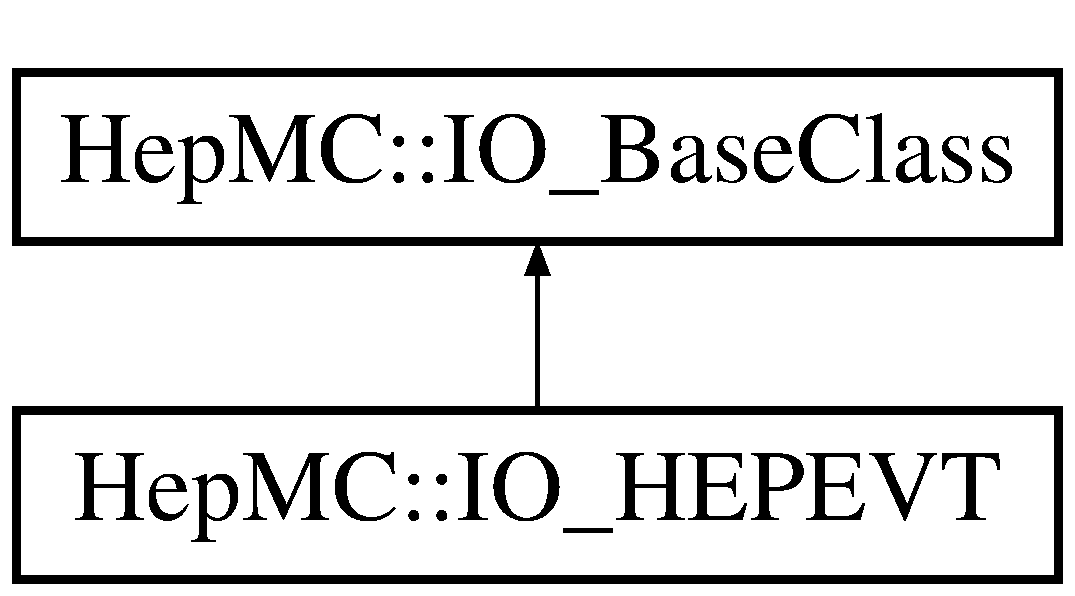
\includegraphics[height=2cm]{classHepMC_1_1IO__HEPEVT}
\end{center}
\end{figure}
\subsection*{Public Member Functions}
\begin{CompactItemize}
\item 
{\bf IO\_\-HEPEVT} ()
\item 
virtual {\bf $\sim$IO\_\-HEPEVT} ()
\item 
bool {\bf fill\_\-next\_\-event} ({\bf Gen\-Event} $\ast$)
\begin{CompactList}\small\item\em fill this \doxyref{Gen\-Event}{p.}{classHepMC_1_1GenEvent} \item\end{CompactList}\item 
void {\bf write\_\-event} (const {\bf Gen\-Event} $\ast$)
\begin{CompactList}\small\item\em write this \doxyref{Gen\-Event}{p.}{classHepMC_1_1GenEvent} \item\end{CompactList}\item 
void {\bf print} (std::ostream \&ostr=std::cout) const
\begin{CompactList}\small\item\em write output to ostr \item\end{CompactList}\item 
bool {\bf trust\_\-both\_\-mothers\_\-and\_\-daughters} () const
\begin{CompactList}\small\item\em default is false \item\end{CompactList}\item 
bool {\bf trust\_\-mothers\_\-before\_\-daughters} () const
\begin{CompactList}\small\item\em default is true \item\end{CompactList}\item 
bool {\bf print\_\-inconsistency\_\-errors} () const
\begin{CompactList}\small\item\em default is true \item\end{CompactList}\item 
void {\bf set\_\-trust\_\-mothers\_\-before\_\-daughters} (bool b=1)
\begin{CompactList}\small\item\em define mother daughter trust rules \item\end{CompactList}\item 
void {\bf set\_\-trust\_\-both\_\-mothers\_\-and\_\-daughters} (bool b=0)
\begin{CompactList}\small\item\em define mother daughter trust rules \item\end{CompactList}\item 
void {\bf set\_\-print\_\-inconsistency\_\-errors} (bool b=1)
\end{CompactItemize}
\subsection*{Protected Member Functions}
\begin{CompactItemize}
\item 
{\bf Gen\-Particle} $\ast$ {\bf build\_\-particle} (int index)
\begin{CompactList}\small\item\em create a \doxyref{Gen\-Particle}{p.}{classHepMC_1_1GenParticle} \item\end{CompactList}\item 
void {\bf build\_\-production\_\-vertex} (int i, std::vector$<$ {\bf Hep\-MC::Gen\-Particle} $\ast$ $>$ \&hepevt\_\-particle, {\bf Gen\-Event} $\ast$evt)
\begin{CompactList}\small\item\em create a production vertex \item\end{CompactList}\item 
void {\bf build\_\-end\_\-vertex} (int i, std::vector$<$ {\bf Hep\-MC::Gen\-Particle} $\ast$ $>$ \&hepevt\_\-particle, {\bf Gen\-Event} $\ast$evt)
\begin{CompactList}\small\item\em create an end vertex \item\end{CompactList}\item 
int {\bf find\_\-in\_\-map} (const std::map$<$ {\bf Hep\-MC::Gen\-Particle} $\ast$, int $>$ \&m, {\bf Gen\-Particle} $\ast${\bf p}) const
\begin{CompactList}\small\item\em find this particle in the particle map \item\end{CompactList}\end{CompactItemize}


\subsection{Detailed Description}
HEPEVT IO class. 

IO class for reading the standard HEPEVT common block. \begin{Desc}
\item[Examples: ]\par


{\bf example\_\-My\-Pythia.cc}, {\bf example\_\-My\-Pythia\-Only\-To\-Hep\-MC.cc}, {\bf example\_\-My\-Pythia\-Read.cc}, {\bf example\_\-My\-Pythia\-With\-Event\-Selection.cc}, and {\bf example\_\-Pythia\-Particle.cc}.\end{Desc}




Definition at line 40 of file IO\_\-HEPEVT.h.

\subsection{Constructor \& Destructor Documentation}
\index{HepMC::IO_HEPEVT@{Hep\-MC::IO\_\-HEPEVT}!IO_HEPEVT@{IO\_\-HEPEVT}}
\index{IO_HEPEVT@{IO\_\-HEPEVT}!HepMC::IO_HEPEVT@{Hep\-MC::IO\_\-HEPEVT}}
\subsubsection{\setlength{\rightskip}{0pt plus 5cm}Hep\-MC::IO\_\-HEPEVT::IO\_\-HEPEVT ()}\label{classHepMC_1_1IO__HEPEVT_7dea9c152eb6ab319411970dc1d95c67}




Definition at line 12 of file IO\_\-HEPEVT.cc.\index{HepMC::IO_HEPEVT@{Hep\-MC::IO\_\-HEPEVT}!~IO_HEPEVT@{$\sim$IO\_\-HEPEVT}}
\index{~IO_HEPEVT@{$\sim$IO\_\-HEPEVT}!HepMC::IO_HEPEVT@{Hep\-MC::IO\_\-HEPEVT}}
\subsubsection{\setlength{\rightskip}{0pt plus 5cm}Hep\-MC::IO\_\-HEPEVT::$\sim$IO\_\-HEPEVT ()\hspace{0.3cm}{\tt  [virtual]}}\label{classHepMC_1_1IO__HEPEVT_f40f251c95a978a24309b57e4d3c06d8}




Definition at line 17 of file IO\_\-HEPEVT.cc.

\subsection{Member Function Documentation}
\index{HepMC::IO_HEPEVT@{Hep\-MC::IO\_\-HEPEVT}!fill_next_event@{fill\_\-next\_\-event}}
\index{fill_next_event@{fill\_\-next\_\-event}!HepMC::IO_HEPEVT@{Hep\-MC::IO\_\-HEPEVT}}
\subsubsection{\setlength{\rightskip}{0pt plus 5cm}bool Hep\-MC::IO\_\-HEPEVT::fill\_\-next\_\-event ({\bf Gen\-Event} $\ast$)\hspace{0.3cm}{\tt  [virtual]}}\label{classHepMC_1_1IO__HEPEVT_e4bcb5527c18d161c11edd19bad49416}


fill this \doxyref{Gen\-Event}{p.}{classHepMC_1_1GenEvent} 



Implements {\bf Hep\-MC::IO\_\-Base\-Class} \doxyref{}{p.}{classHepMC_1_1IO__BaseClass_f1dffb95a44d521af510f6431a30f942}.

Definition at line 30 of file IO\_\-HEPEVT.cc.

References Hep\-MC::Gen\-Vertex::add\_\-particle\_\-out(), Hep\-MC::Gen\-Event::add\_\-vertex(), build\_\-end\_\-vertex(), build\_\-particle(), build\_\-production\_\-vertex(), Hep\-MC::HEPEVT\_\-Wrapper::event\_\-number(), Hep\-MC::HEPEVT\_\-Wrapper::number\_\-entries(), Hep\-MC::Gen\-Event::set\_\-beam\_\-particles(), and Hep\-MC::Gen\-Event::set\_\-event\_\-number().\index{HepMC::IO_HEPEVT@{Hep\-MC::IO\_\-HEPEVT}!write_event@{write\_\-event}}
\index{write_event@{write\_\-event}!HepMC::IO_HEPEVT@{Hep\-MC::IO\_\-HEPEVT}}
\subsubsection{\setlength{\rightskip}{0pt plus 5cm}void Hep\-MC::IO\_\-HEPEVT::write\_\-event (const {\bf Gen\-Event} $\ast$)\hspace{0.3cm}{\tt  [virtual]}}\label{classHepMC_1_1IO__HEPEVT_adbd36a8914a4cc275be26856884da43}


write this \doxyref{Gen\-Event}{p.}{classHepMC_1_1GenEvent} 



Implements {\bf Hep\-MC::IO\_\-Base\-Class} \doxyref{}{p.}{classHepMC_1_1IO__BaseClass_7929dfd8412207c7904f29652810c1f4}.

Definition at line 107 of file IO\_\-HEPEVT.cc.

References Hep\-MC::Four\-Vector::e(), Hep\-MC::Gen\-Event::event\_\-number(), find\_\-in\_\-map(), Hep\-MC::HEPEVT\_\-Wrapper::max\_\-number\_\-entries(), p, Hep\-MC::Four\-Vector::px(), Hep\-MC::Four\-Vector::py(), Hep\-MC::Four\-Vector::pz(), Hep\-MC::HEPEVT\_\-Wrapper::set\_\-children(), Hep\-MC::HEPEVT\_\-Wrapper::set\_\-event\_\-number(), Hep\-MC::HEPEVT\_\-Wrapper::set\_\-id(), Hep\-MC::HEPEVT\_\-Wrapper::set\_\-mass(), Hep\-MC::HEPEVT\_\-Wrapper::set\_\-momentum(), Hep\-MC::HEPEVT\_\-Wrapper::set\_\-number\_\-entries(), Hep\-MC::HEPEVT\_\-Wrapper::set\_\-parents(), Hep\-MC::HEPEVT\_\-Wrapper::set\_\-position(), Hep\-MC::HEPEVT\_\-Wrapper::set\_\-status(), v, Hep\-MC::Gen\-Event::vertices\_\-begin(), and Hep\-MC::Gen\-Event::vertices\_\-end().\index{HepMC::IO_HEPEVT@{Hep\-MC::IO\_\-HEPEVT}!print@{print}}
\index{print@{print}!HepMC::IO_HEPEVT@{Hep\-MC::IO\_\-HEPEVT}}
\subsubsection{\setlength{\rightskip}{0pt plus 5cm}void Hep\-MC::IO\_\-HEPEVT::print (std::ostream \& {\em ostr} = {\tt std::cout}) const\hspace{0.3cm}{\tt  [virtual]}}\label{classHepMC_1_1IO__HEPEVT_5f360aa251e909cc77f1a9f9d45d7abf}


write output to ostr 



Reimplemented from {\bf Hep\-MC::IO\_\-Base\-Class} \doxyref{}{p.}{classHepMC_1_1IO__BaseClass_52a1503f4107fd3d5f4da02feb45751b}.

Definition at line 19 of file IO\_\-HEPEVT.cc.\index{HepMC::IO_HEPEVT@{Hep\-MC::IO\_\-HEPEVT}!trust_both_mothers_and_daughters@{trust\_\-both\_\-mothers\_\-and\_\-daughters}}
\index{trust_both_mothers_and_daughters@{trust\_\-both\_\-mothers\_\-and\_\-daughters}!HepMC::IO_HEPEVT@{Hep\-MC::IO\_\-HEPEVT}}
\subsubsection{\setlength{\rightskip}{0pt plus 5cm}bool Hep\-MC::IO\_\-HEPEVT::trust\_\-both\_\-mothers\_\-and\_\-daughters () const\hspace{0.3cm}{\tt  [inline]}}\label{classHepMC_1_1IO__HEPEVT_da542868612c376e1fa1adb94deab118}


default is false 



Definition at line 115 of file IO\_\-HEPEVT.h.\index{HepMC::IO_HEPEVT@{Hep\-MC::IO\_\-HEPEVT}!trust_mothers_before_daughters@{trust\_\-mothers\_\-before\_\-daughters}}
\index{trust_mothers_before_daughters@{trust\_\-mothers\_\-before\_\-daughters}!HepMC::IO_HEPEVT@{Hep\-MC::IO\_\-HEPEVT}}
\subsubsection{\setlength{\rightskip}{0pt plus 5cm}bool Hep\-MC::IO\_\-HEPEVT::trust\_\-mothers\_\-before\_\-daughters () const\hspace{0.3cm}{\tt  [inline]}}\label{classHepMC_1_1IO__HEPEVT_73e69f77a8f127f43d8c445654c78f53}


default is true 



Definition at line 118 of file IO\_\-HEPEVT.h.\index{HepMC::IO_HEPEVT@{Hep\-MC::IO\_\-HEPEVT}!print_inconsistency_errors@{print\_\-inconsistency\_\-errors}}
\index{print_inconsistency_errors@{print\_\-inconsistency\_\-errors}!HepMC::IO_HEPEVT@{Hep\-MC::IO\_\-HEPEVT}}
\subsubsection{\setlength{\rightskip}{0pt plus 5cm}bool Hep\-MC::IO\_\-HEPEVT::print\_\-inconsistency\_\-errors () const\hspace{0.3cm}{\tt  [inline]}}\label{classHepMC_1_1IO__HEPEVT_12b8af7dadcf207441f6822a288f7d99}


default is true 



Definition at line 121 of file IO\_\-HEPEVT.h.\index{HepMC::IO_HEPEVT@{Hep\-MC::IO\_\-HEPEVT}!set_trust_mothers_before_daughters@{set\_\-trust\_\-mothers\_\-before\_\-daughters}}
\index{set_trust_mothers_before_daughters@{set\_\-trust\_\-mothers\_\-before\_\-daughters}!HepMC::IO_HEPEVT@{Hep\-MC::IO\_\-HEPEVT}}
\subsubsection{\setlength{\rightskip}{0pt plus 5cm}void Hep\-MC::IO\_\-HEPEVT::set\_\-trust\_\-mothers\_\-before\_\-daughters (bool {\em b} = {\tt 1})\hspace{0.3cm}{\tt  [inline]}}\label{classHepMC_1_1IO__HEPEVT_edf281b976c43518477f5a854f466055}


define mother daughter trust rules 



Definition at line 127 of file IO\_\-HEPEVT.h.\index{HepMC::IO_HEPEVT@{Hep\-MC::IO\_\-HEPEVT}!set_trust_both_mothers_and_daughters@{set\_\-trust\_\-both\_\-mothers\_\-and\_\-daughters}}
\index{set_trust_both_mothers_and_daughters@{set\_\-trust\_\-both\_\-mothers\_\-and\_\-daughters}!HepMC::IO_HEPEVT@{Hep\-MC::IO\_\-HEPEVT}}
\subsubsection{\setlength{\rightskip}{0pt plus 5cm}void Hep\-MC::IO\_\-HEPEVT::set\_\-trust\_\-both\_\-mothers\_\-and\_\-daughters (bool {\em b} = {\tt 0})\hspace{0.3cm}{\tt  [inline]}}\label{classHepMC_1_1IO__HEPEVT_69638656feb93fadd49c5fb49de85169}


define mother daughter trust rules 



Definition at line 124 of file IO\_\-HEPEVT.h.\index{HepMC::IO_HEPEVT@{Hep\-MC::IO\_\-HEPEVT}!set_print_inconsistency_errors@{set\_\-print\_\-inconsistency\_\-errors}}
\index{set_print_inconsistency_errors@{set\_\-print\_\-inconsistency\_\-errors}!HepMC::IO_HEPEVT@{Hep\-MC::IO\_\-HEPEVT}}
\subsubsection{\setlength{\rightskip}{0pt plus 5cm}void Hep\-MC::IO\_\-HEPEVT::set\_\-print\_\-inconsistency\_\-errors (bool {\em b} = {\tt 1})\hspace{0.3cm}{\tt  [inline]}}\label{classHepMC_1_1IO__HEPEVT_45cd7df10900c29cad418546040bdce7}


Since HEPEVT has bi-directional pointers, it is possible that the mother/daughter pointers are inconsistent (though physically speaking this should never happen). In practise it happens often. When a conflict occurs (i.e. when mother/daughter pointers are in disagreement, where an empty (0) pointer is not considered a disagreement) an error is printed. These errors can be turned off with: myio\_\-hepevt.set\_\-print\_\-inconsistency\_\-errors(0); but it is STRONGLY recommended that you print the HEPEVT common and understand the inconsistency BEFORE you turn off the errors. The messages are there for a reason [remember, there is no message printed when the information is missing, ... only when is it inconsistent. User beware.] You can inspect the HEPEVT common block for inconsistencies with \doxyref{HEPEVT\_\-Wrapper::check\_\-hepevt\_\-consistency()}{p.}{classHepMC_1_1HEPEVT__Wrapper_b9425bd4b1ba5dbcc21b3716c74350a4}

There is a switch controlling whether the mother pointers or the daughters are to be trusted. For example, in Pythia the mother information is always correctly included, but the daughter information is often left unfilled: in this case we want to trust the mother pointers and not necessarily the daughters. [THIS IS THE DEFAULT]. Unfortunately the reverse happens for the stdhep(2001) translation of Isajet, so we need an option to toggle the choices. 

Definition at line 130 of file IO\_\-HEPEVT.h.\index{HepMC::IO_HEPEVT@{Hep\-MC::IO\_\-HEPEVT}!build_particle@{build\_\-particle}}
\index{build_particle@{build\_\-particle}!HepMC::IO_HEPEVT@{Hep\-MC::IO\_\-HEPEVT}}
\subsubsection{\setlength{\rightskip}{0pt plus 5cm}{\bf Gen\-Particle} $\ast$ Hep\-MC::IO\_\-HEPEVT::build\_\-particle (int {\em index})\hspace{0.3cm}{\tt  [protected]}}\label{classHepMC_1_1IO__HEPEVT_b042bd93c5342be41189f13b270a4d65}


create a \doxyref{Gen\-Particle}{p.}{classHepMC_1_1GenParticle} 



Builds a particle object corresponding to index in HEPEVT 

Definition at line 319 of file IO\_\-HEPEVT.cc.

References Hep\-MC::HEPEVT\_\-Wrapper::e(), Hep\-MC::HEPEVT\_\-Wrapper::id(), Hep\-MC::HEPEVT\_\-Wrapper::m(), p, Hep\-MC::HEPEVT\_\-Wrapper::px(), Hep\-MC::HEPEVT\_\-Wrapper::py(), Hep\-MC::HEPEVT\_\-Wrapper::pz(), and Hep\-MC::HEPEVT\_\-Wrapper::status().

Referenced by fill\_\-next\_\-event().\index{HepMC::IO_HEPEVT@{Hep\-MC::IO\_\-HEPEVT}!build_production_vertex@{build\_\-production\_\-vertex}}
\index{build_production_vertex@{build\_\-production\_\-vertex}!HepMC::IO_HEPEVT@{Hep\-MC::IO\_\-HEPEVT}}
\subsubsection{\setlength{\rightskip}{0pt plus 5cm}void Hep\-MC::IO\_\-HEPEVT::build\_\-production\_\-vertex (int {\em i}, std::vector$<$ {\bf Hep\-MC::Gen\-Particle} $\ast$ $>$ \& {\em hepevt\_\-particle}, {\bf Gen\-Event} $\ast$ {\em evt})\hspace{0.3cm}{\tt  [protected]}}\label{classHepMC_1_1IO__HEPEVT_c3fdc9b74869cef1d8be1ade1deae92e}


create a production vertex 



Referenced by fill\_\-next\_\-event().\index{HepMC::IO_HEPEVT@{Hep\-MC::IO\_\-HEPEVT}!build_end_vertex@{build\_\-end\_\-vertex}}
\index{build_end_vertex@{build\_\-end\_\-vertex}!HepMC::IO_HEPEVT@{Hep\-MC::IO\_\-HEPEVT}}
\subsubsection{\setlength{\rightskip}{0pt plus 5cm}void Hep\-MC::IO\_\-HEPEVT::build\_\-end\_\-vertex (int {\em i}, std::vector$<$ {\bf Hep\-MC::Gen\-Particle} $\ast$ $>$ \& {\em hepevt\_\-particle}, {\bf Gen\-Event} $\ast$ {\em evt})\hspace{0.3cm}{\tt  [protected]}}\label{classHepMC_1_1IO__HEPEVT_cbb0df9903cfabaef93a6df00f9ce917}


create an end vertex 



Referenced by fill\_\-next\_\-event().\index{HepMC::IO_HEPEVT@{Hep\-MC::IO\_\-HEPEVT}!find_in_map@{find\_\-in\_\-map}}
\index{find_in_map@{find\_\-in\_\-map}!HepMC::IO_HEPEVT@{Hep\-MC::IO\_\-HEPEVT}}
\subsubsection{\setlength{\rightskip}{0pt plus 5cm}int Hep\-MC::IO\_\-HEPEVT::find\_\-in\_\-map (const std::map$<$ {\bf Hep\-MC::Gen\-Particle} $\ast$, int $>$ \& {\em m}, {\bf Gen\-Particle} $\ast$ {\em p}) const\hspace{0.3cm}{\tt  [protected]}}\label{classHepMC_1_1IO__HEPEVT_a5c410137397079e6df0426eb39d2027}


find this particle in the particle map 



Referenced by write\_\-event().

The documentation for this class was generated from the following files:\begin{CompactItemize}
\item 
{\bf IO\_\-HEPEVT.h}\item 
{\bf IO\_\-HEPEVT.cc}\end{CompactItemize}

\section{Hep\-MC::IO\_\-HERWIG Class Reference}
\label{classHepMC_1_1IO__HERWIG}\index{HepMC::IO_HERWIG@{HepMC::IO\_\-HERWIG}}
\doxyref{IO\_\-HERWIG}{p.}{classHepMC_1_1IO__HERWIG} is used to get Herwig information.  


{\tt \#include $<$IO\_\-HERWIG.h$>$}

Inheritance diagram for Hep\-MC::IO\_\-HERWIG::\begin{figure}[H]
\begin{center}
\leavevmode
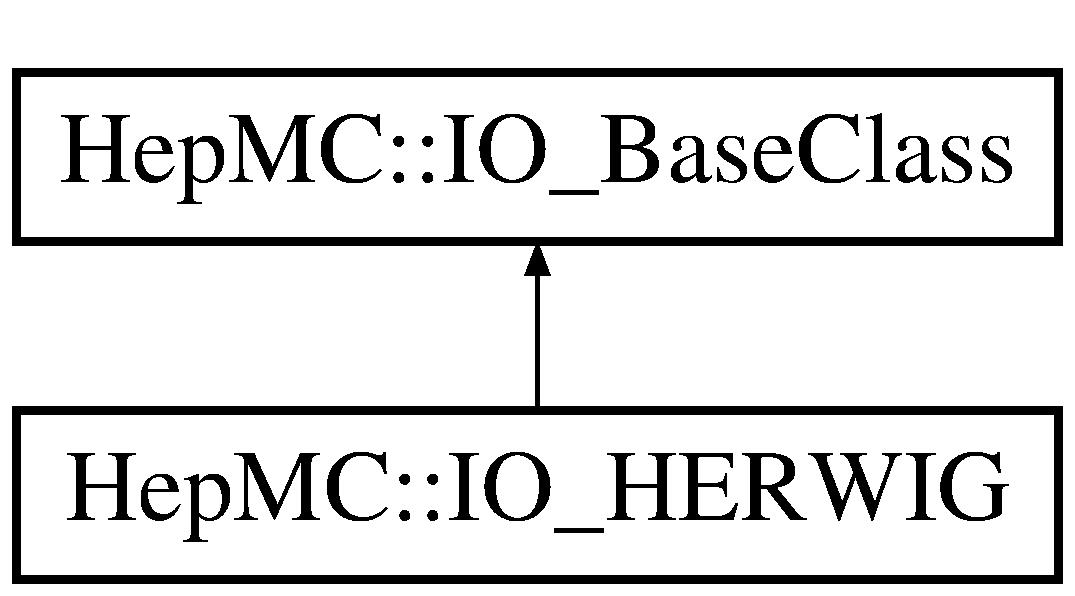
\includegraphics[height=2cm]{classHepMC_1_1IO__HERWIG}
\end{center}
\end{figure}
\subsection*{Public Member Functions}
\begin{CompactItemize}
\item 
{\bf IO\_\-HERWIG} ()
\item 
virtual {\bf $\sim$IO\_\-HERWIG} ()
\item 
bool {\bf fill\_\-next\_\-event} ({\bf Gen\-Event} $\ast$)
\begin{CompactList}\small\item\em get the next event \item\end{CompactList}\item 
void {\bf print} (std::ostream \&ostr=std::cout) const
\begin{CompactList}\small\item\em write to ostr \item\end{CompactList}\item 
double {\bf interfaces\_\-to\_\-version\_\-number} () const
\begin{CompactList}\small\item\em this information is dubious \item\end{CompactList}\item 
bool {\bf print\_\-inconsistency\_\-errors} () const
\begin{CompactList}\small\item\em default is true \item\end{CompactList}\item 
void {\bf set\_\-print\_\-inconsistency\_\-errors} (bool b=1)
\begin{CompactList}\small\item\em decide whether or not to print inconsistency errors \item\end{CompactList}\item 
bool {\bf no\_\-gaps\_\-in\_\-barcodes} () const
\begin{CompactList}\small\item\em ask how to deal with extra non-physical pseudo particles \item\end{CompactList}\item 
void {\bf set\_\-no\_\-gaps\_\-in\_\-barcodes} (bool a)
\end{CompactItemize}
\subsection*{Protected Member Functions}
\begin{CompactItemize}
\item 
bool {\bf trust\_\-both\_\-mothers\_\-and\_\-daughters} () const
\begin{CompactList}\small\item\em default is true \item\end{CompactList}\item 
bool {\bf trust\_\-mothers\_\-before\_\-daughters} () const
\begin{CompactList}\small\item\em default is false \item\end{CompactList}\item 
void {\bf set\_\-trust\_\-mothers\_\-before\_\-daughters} (bool b=1)
\begin{CompactList}\small\item\em define mother daughter trust rules \item\end{CompactList}\item 
void {\bf set\_\-trust\_\-both\_\-mothers\_\-and\_\-daughters} (bool b=0)
\begin{CompactList}\small\item\em define mother daughter trust rules \item\end{CompactList}\item 
{\bf Gen\-Particle} $\ast$ {\bf build\_\-particle} (int index)
\begin{CompactList}\small\item\em make a particle \item\end{CompactList}\item 
void {\bf build\_\-production\_\-vertex} (int i, std::vector$<$ {\bf Gen\-Particle} $\ast$ $>$ \&hepevt\_\-particle, {\bf Gen\-Event} $\ast$evt)
\begin{CompactList}\small\item\em make a production vertex \item\end{CompactList}\item 
void {\bf build\_\-end\_\-vertex} (int i, std::vector$<$ {\bf Gen\-Particle} $\ast$ $>$ \&hepevt\_\-particle, {\bf Gen\-Event} $\ast$evt)
\begin{CompactList}\small\item\em make a decay vertex \item\end{CompactList}\item 
int {\bf find\_\-in\_\-map} (const std::map$<$ {\bf Gen\-Particle} $\ast$, int $>$ \&m, {\bf Gen\-Particle} $\ast${\bf p}) const
\begin{CompactList}\small\item\em find this particle in the map \item\end{CompactList}\item 
void {\bf repair\_\-hepevt} () const
\begin{CompactList}\small\item\em make the HERWIG HEPEVT common block look like the standard \item\end{CompactList}\item 
void {\bf remove\_\-gaps\_\-in\_\-hepevt} () const
\begin{CompactList}\small\item\em deal with artifacts of repairing HEPEVT \item\end{CompactList}\item 
void {\bf zero\_\-hepevt\_\-entry} (int i) const
\begin{CompactList}\small\item\em zero out a HEPEVT pseudo particle \item\end{CompactList}\item 
int {\bf translate\_\-herwig\_\-to\_\-pdg\_\-id} (int i) const
\begin{CompactList}\small\item\em translate particle ID \item\end{CompactList}\end{CompactItemize}


\subsection{Detailed Description}
\doxyref{IO\_\-HERWIG}{p.}{classHepMC_1_1IO__HERWIG} is used to get Herwig information. 

IO class for reading the HEPEVT common block from the Herwig monte carlo program. \begin{Desc}
\item[Examples: ]\par


{\bf example\_\-My\-Herwig.cc}.\end{Desc}




Definition at line 57 of file IO\_\-HERWIG.h.

\subsection{Constructor \& Destructor Documentation}
\index{HepMC::IO_HERWIG@{Hep\-MC::IO\_\-HERWIG}!IO_HERWIG@{IO\_\-HERWIG}}
\index{IO_HERWIG@{IO\_\-HERWIG}!HepMC::IO_HERWIG@{Hep\-MC::IO\_\-HERWIG}}
\subsubsection{\setlength{\rightskip}{0pt plus 5cm}Hep\-MC::IO\_\-HERWIG::IO\_\-HERWIG ()}\label{classHepMC_1_1IO__HERWIG_b301cc044feaf12ebbd0f3e3d2bd170a}




Definition at line 12 of file IO\_\-HERWIG.cc.\index{HepMC::IO_HERWIG@{Hep\-MC::IO\_\-HERWIG}!~IO_HERWIG@{$\sim$IO\_\-HERWIG}}
\index{~IO_HERWIG@{$\sim$IO\_\-HERWIG}!HepMC::IO_HERWIG@{Hep\-MC::IO\_\-HERWIG}}
\subsubsection{\setlength{\rightskip}{0pt plus 5cm}Hep\-MC::IO\_\-HERWIG::$\sim$IO\_\-HERWIG ()\hspace{0.3cm}{\tt  [virtual]}}\label{classHepMC_1_1IO__HERWIG_99bfa883ae364b1154c8cc7dc7d311a0}




Definition at line 81 of file IO\_\-HERWIG.cc.

\subsection{Member Function Documentation}
\index{HepMC::IO_HERWIG@{Hep\-MC::IO\_\-HERWIG}!fill_next_event@{fill\_\-next\_\-event}}
\index{fill_next_event@{fill\_\-next\_\-event}!HepMC::IO_HERWIG@{Hep\-MC::IO\_\-HERWIG}}
\subsubsection{\setlength{\rightskip}{0pt plus 5cm}bool Hep\-MC::IO\_\-HERWIG::fill\_\-next\_\-event ({\bf Gen\-Event} $\ast$)\hspace{0.3cm}{\tt  [virtual]}}\label{classHepMC_1_1IO__HERWIG_7a49968897062f0e977053bcdf176e17}


get the next event 



read one event from the Herwig HEPEVT common block and fill \doxyref{Gen\-Event}{p.}{classHepMC_1_1GenEvent} return T/F =success/failure

sufficient to do one or the other. 

Implements {\bf Hep\-MC::IO\_\-Base\-Class} \doxyref{}{p.}{classHepMC_1_1IO__BaseClass_f1dffb95a44d521af510f6431a30f942}.

Definition at line 94 of file IO\_\-HERWIG.cc.

References Hep\-MC::Gen\-Vertex::add\_\-particle\_\-in(), Hep\-MC::Gen\-Vertex::add\_\-particle\_\-out(), Hep\-MC::Gen\-Event::add\_\-vertex(), build\_\-end\_\-vertex(), build\_\-particle(), build\_\-production\_\-vertex(), Hep\-MC::HEPEVT\_\-Wrapper::event\_\-number(), Hep\-MC::HEPEVT\_\-Wrapper::number\_\-entries(), repair\_\-hepevt(), Hep\-MC::Gen\-Event::set\_\-beam\_\-particles(), Hep\-MC::Gen\-Event::set\_\-event\_\-number(), Hep\-MC::Gen\-Event::set\_\-signal\_\-process\_\-vertex(), and Hep\-MC::HEPEVT\_\-Wrapper::status().\index{HepMC::IO_HERWIG@{Hep\-MC::IO\_\-HERWIG}!print@{print}}
\index{print@{print}!HepMC::IO_HERWIG@{Hep\-MC::IO\_\-HERWIG}}
\subsubsection{\setlength{\rightskip}{0pt plus 5cm}void Hep\-MC::IO\_\-HERWIG::print (std::ostream \& {\em ostr} = {\tt std::cout}) const\hspace{0.3cm}{\tt  [virtual]}}\label{classHepMC_1_1IO__HERWIG_ab6853a2888f6e2f628039b9079fe120}


write to ostr 



Reimplemented from {\bf Hep\-MC::IO\_\-Base\-Class} \doxyref{}{p.}{classHepMC_1_1IO__BaseClass_52a1503f4107fd3d5f4da02feb45751b}.

Definition at line 83 of file IO\_\-HERWIG.cc.\index{HepMC::IO_HERWIG@{Hep\-MC::IO\_\-HERWIG}!interfaces_to_version_number@{interfaces\_\-to\_\-version\_\-number}}
\index{interfaces_to_version_number@{interfaces\_\-to\_\-version\_\-number}!HepMC::IO_HERWIG@{Hep\-MC::IO\_\-HERWIG}}
\subsubsection{\setlength{\rightskip}{0pt plus 5cm}double Hep\-MC::IO\_\-HERWIG::interfaces\_\-to\_\-version\_\-number () const\hspace{0.3cm}{\tt  [inline]}}\label{classHepMC_1_1IO__HERWIG_a527cb458b5c699b51f68a22bb72cf08}


this information is dubious 



Definition at line 66 of file IO\_\-HERWIG.h.\index{HepMC::IO_HERWIG@{Hep\-MC::IO\_\-HERWIG}!print_inconsistency_errors@{print\_\-inconsistency\_\-errors}}
\index{print_inconsistency_errors@{print\_\-inconsistency\_\-errors}!HepMC::IO_HERWIG@{Hep\-MC::IO\_\-HERWIG}}
\subsubsection{\setlength{\rightskip}{0pt plus 5cm}bool Hep\-MC::IO\_\-HERWIG::print\_\-inconsistency\_\-errors () const\hspace{0.3cm}{\tt  [inline]}}\label{classHepMC_1_1IO__HERWIG_2c9a32518c8520046758ca9c96c7a909}


default is true 



Definition at line 149 of file IO\_\-HERWIG.h.\index{HepMC::IO_HERWIG@{Hep\-MC::IO\_\-HERWIG}!set_print_inconsistency_errors@{set\_\-print\_\-inconsistency\_\-errors}}
\index{set_print_inconsistency_errors@{set\_\-print\_\-inconsistency\_\-errors}!HepMC::IO_HERWIG@{Hep\-MC::IO\_\-HERWIG}}
\subsubsection{\setlength{\rightskip}{0pt plus 5cm}void Hep\-MC::IO\_\-HERWIG::set\_\-print\_\-inconsistency\_\-errors (bool {\em b} = {\tt 1})\hspace{0.3cm}{\tt  [inline]}}\label{classHepMC_1_1IO__HERWIG_d11799a2ca5e3597057b31e278dca4ef}


decide whether or not to print inconsistency errors 



Definition at line 158 of file IO\_\-HERWIG.h.\index{HepMC::IO_HERWIG@{Hep\-MC::IO\_\-HERWIG}!no_gaps_in_barcodes@{no\_\-gaps\_\-in\_\-barcodes}}
\index{no_gaps_in_barcodes@{no\_\-gaps\_\-in\_\-barcodes}!HepMC::IO_HERWIG@{Hep\-MC::IO\_\-HERWIG}}
\subsubsection{\setlength{\rightskip}{0pt plus 5cm}bool Hep\-MC::IO\_\-HERWIG::no\_\-gaps\_\-in\_\-barcodes () const\hspace{0.3cm}{\tt  [inline]}}\label{classHepMC_1_1IO__HERWIG_7d8d7242a83f0185b53817793cbc1186}


ask how to deal with extra non-physical pseudo particles 



Definition at line 75 of file IO\_\-HERWIG.h.\index{HepMC::IO_HERWIG@{Hep\-MC::IO\_\-HERWIG}!set_no_gaps_in_barcodes@{set\_\-no\_\-gaps\_\-in\_\-barcodes}}
\index{set_no_gaps_in_barcodes@{set\_\-no\_\-gaps\_\-in\_\-barcodes}!HepMC::IO_HERWIG@{Hep\-MC::IO\_\-HERWIG}}
\subsubsection{\setlength{\rightskip}{0pt plus 5cm}void Hep\-MC::IO\_\-HERWIG::set\_\-no\_\-gaps\_\-in\_\-barcodes (bool {\em a})\hspace{0.3cm}{\tt  [inline]}}\label{classHepMC_1_1IO__HERWIG_0f796aa2819af640479f914524549697}


The HERWIG HEPEVT common block has some EXTRA non-physical ENTRIES (such as CMS frame, HARD subprocess, and CONE). These are removed by \doxyref{IO\_\-HERWIG}{p.}{classHepMC_1_1IO__HERWIG}. Thus the \doxyref{Hep\-MC}{p.}{namespaceHepMC} event will APPEAR to have fewer particles in it that herwig did. There is a switch m\_\-no\_\-gaps\_\-in\_\-barcodes. For true - then the extra particles are removed from HEPEVT, with the result that the \doxyref{Hep\-MC}{p.}{namespaceHepMC} barcodes will be sequential, with no gaps. false - the barcodes will correspond directly to the HEPEVT index, but there will be gaps ... ie some barcodes will be unassigned. this switch requested by I Hinchliffe, October 31, 2002 

Definition at line 88 of file IO\_\-HERWIG.h.\index{HepMC::IO_HERWIG@{Hep\-MC::IO\_\-HERWIG}!trust_both_mothers_and_daughters@{trust\_\-both\_\-mothers\_\-and\_\-daughters}}
\index{trust_both_mothers_and_daughters@{trust\_\-both\_\-mothers\_\-and\_\-daughters}!HepMC::IO_HERWIG@{Hep\-MC::IO\_\-HERWIG}}
\subsubsection{\setlength{\rightskip}{0pt plus 5cm}bool Hep\-MC::IO\_\-HERWIG::trust\_\-both\_\-mothers\_\-and\_\-daughters () const\hspace{0.3cm}{\tt  [inline, protected]}}\label{classHepMC_1_1IO__HERWIG_d9e2a90df8aca3e22d82e27314834745}


default is true 



Definition at line 143 of file IO\_\-HERWIG.h.\index{HepMC::IO_HERWIG@{Hep\-MC::IO\_\-HERWIG}!trust_mothers_before_daughters@{trust\_\-mothers\_\-before\_\-daughters}}
\index{trust_mothers_before_daughters@{trust\_\-mothers\_\-before\_\-daughters}!HepMC::IO_HERWIG@{Hep\-MC::IO\_\-HERWIG}}
\subsubsection{\setlength{\rightskip}{0pt plus 5cm}bool Hep\-MC::IO\_\-HERWIG::trust\_\-mothers\_\-before\_\-daughters () const\hspace{0.3cm}{\tt  [inline, protected]}}\label{classHepMC_1_1IO__HERWIG_fb49848889fa6fb602c98f573c565f64}


default is false 



Definition at line 146 of file IO\_\-HERWIG.h.\index{HepMC::IO_HERWIG@{Hep\-MC::IO\_\-HERWIG}!set_trust_mothers_before_daughters@{set\_\-trust\_\-mothers\_\-before\_\-daughters}}
\index{set_trust_mothers_before_daughters@{set\_\-trust\_\-mothers\_\-before\_\-daughters}!HepMC::IO_HERWIG@{Hep\-MC::IO\_\-HERWIG}}
\subsubsection{\setlength{\rightskip}{0pt plus 5cm}void Hep\-MC::IO\_\-HERWIG::set\_\-trust\_\-mothers\_\-before\_\-daughters (bool {\em b} = {\tt 1})\hspace{0.3cm}{\tt  [inline, protected]}}\label{classHepMC_1_1IO__HERWIG_909da8fafb3bf468e8547d7d0fac7f67}


define mother daughter trust rules 



Definition at line 155 of file IO\_\-HERWIG.h.\index{HepMC::IO_HERWIG@{Hep\-MC::IO\_\-HERWIG}!set_trust_both_mothers_and_daughters@{set\_\-trust\_\-both\_\-mothers\_\-and\_\-daughters}}
\index{set_trust_both_mothers_and_daughters@{set\_\-trust\_\-both\_\-mothers\_\-and\_\-daughters}!HepMC::IO_HERWIG@{Hep\-MC::IO\_\-HERWIG}}
\subsubsection{\setlength{\rightskip}{0pt plus 5cm}void Hep\-MC::IO\_\-HERWIG::set\_\-trust\_\-both\_\-mothers\_\-and\_\-daughters (bool {\em b} = {\tt 0})\hspace{0.3cm}{\tt  [inline, protected]}}\label{classHepMC_1_1IO__HERWIG_169a866ff551c5d2f62d48dbff537dec}


define mother daughter trust rules 



Definition at line 152 of file IO\_\-HERWIG.h.\index{HepMC::IO_HERWIG@{Hep\-MC::IO\_\-HERWIG}!build_particle@{build\_\-particle}}
\index{build_particle@{build\_\-particle}!HepMC::IO_HERWIG@{Hep\-MC::IO\_\-HERWIG}}
\subsubsection{\setlength{\rightskip}{0pt plus 5cm}{\bf Gen\-Particle} $\ast$ Hep\-MC::IO\_\-HERWIG::build\_\-particle (int {\em index})\hspace{0.3cm}{\tt  [protected]}}\label{classHepMC_1_1IO__HERWIG_2afff99e4948621126d1211272b3fb02}


make a particle 



Builds a particle object corresponding to index in HEPEVT 

Definition at line 342 of file IO\_\-HERWIG.cc.

References Hep\-MC::HEPEVT\_\-Wrapper::e(), Hep\-MC::HEPEVT\_\-Wrapper::id(), Hep\-MC::HEPEVT\_\-Wrapper::m(), p, Hep\-MC::HEPEVT\_\-Wrapper::px(), Hep\-MC::HEPEVT\_\-Wrapper::py(), Hep\-MC::HEPEVT\_\-Wrapper::pz(), and Hep\-MC::HEPEVT\_\-Wrapper::status().

Referenced by fill\_\-next\_\-event().\index{HepMC::IO_HERWIG@{Hep\-MC::IO\_\-HERWIG}!build_production_vertex@{build\_\-production\_\-vertex}}
\index{build_production_vertex@{build\_\-production\_\-vertex}!HepMC::IO_HERWIG@{Hep\-MC::IO\_\-HERWIG}}
\subsubsection{\setlength{\rightskip}{0pt plus 5cm}void Hep\-MC::IO\_\-HERWIG::build\_\-production\_\-vertex (int {\em i}, std::vector$<$ {\bf Gen\-Particle} $\ast$ $>$ \& {\em hepevt\_\-particle}, {\bf Gen\-Event} $\ast$ {\em evt})\hspace{0.3cm}{\tt  [protected]}}\label{classHepMC_1_1IO__HERWIG_6de881de5bbbf579695522af451814a7}


make a production vertex 



for particle in HEPEVT with index i, build a production vertex if appropriate, and add that vertex to the event 

Definition at line 201 of file IO\_\-HERWIG.cc.

References Hep\-MC::Gen\-Vertex::add\_\-particle\_\-in(), Hep\-MC::Gen\-Vertex::add\_\-particle\_\-out(), Hep\-MC::Gen\-Event::add\_\-vertex(), Hep\-MC::HEPEVT\_\-Wrapper::event\_\-number(), Hep\-MC::HEPEVT\_\-Wrapper::first\_\-parent(), Hep\-MC::HEPEVT\_\-Wrapper::last\_\-parent(), Hep\-MC::HEPEVT\_\-Wrapper::number\_\-parents(), p, Hep\-MC::Gen\-Vertex::position(), Hep\-MC::Gen\-Vertex::print(), Hep\-MC::Gen\-Vertex::set\_\-position(), Hep\-MC::HEPEVT\_\-Wrapper::t(), Hep\-MC::HEPEVT\_\-Wrapper::x(), Hep\-MC::HEPEVT\_\-Wrapper::y(), and Hep\-MC::HEPEVT\_\-Wrapper::z().

Referenced by build\_\-end\_\-vertex(), and fill\_\-next\_\-event().\index{HepMC::IO_HERWIG@{Hep\-MC::IO\_\-HERWIG}!build_end_vertex@{build\_\-end\_\-vertex}}
\index{build_end_vertex@{build\_\-end\_\-vertex}!HepMC::IO_HERWIG@{Hep\-MC::IO\_\-HERWIG}}
\subsubsection{\setlength{\rightskip}{0pt plus 5cm}void Hep\-MC::IO\_\-HERWIG::build\_\-end\_\-vertex (int {\em i}, std::vector$<$ {\bf Gen\-Particle} $\ast$ $>$ \& {\em hepevt\_\-particle}, {\bf Gen\-Event} $\ast$ {\em evt})\hspace{0.3cm}{\tt  [protected]}}\label{classHepMC_1_1IO__HERWIG_8077ede98c4040631f28424c6624a50b}


make a decay vertex 



for particle in HEPEVT with index i, build an end vertex if appropriate, and add that vertex to the event 

Definition at line 274 of file IO\_\-HERWIG.cc.

References Hep\-MC::Gen\-Vertex::add\_\-particle\_\-in(), Hep\-MC::Gen\-Vertex::add\_\-particle\_\-out(), Hep\-MC::Gen\-Event::add\_\-vertex(), build\_\-production\_\-vertex(), Hep\-MC::HEPEVT\_\-Wrapper::event\_\-number(), Hep\-MC::HEPEVT\_\-Wrapper::first\_\-child(), Hep\-MC::HEPEVT\_\-Wrapper::last\_\-child(), Hep\-MC::HEPEVT\_\-Wrapper::number\_\-children(), p, Hep\-MC::Gen\-Vertex::position(), Hep\-MC::Gen\-Vertex::set\_\-position(), Hep\-MC::HEPEVT\_\-Wrapper::t(), Hep\-MC::HEPEVT\_\-Wrapper::x(), Hep\-MC::HEPEVT\_\-Wrapper::y(), and Hep\-MC::HEPEVT\_\-Wrapper::z().

Referenced by fill\_\-next\_\-event().\index{HepMC::IO_HERWIG@{Hep\-MC::IO\_\-HERWIG}!find_in_map@{find\_\-in\_\-map}}
\index{find_in_map@{find\_\-in\_\-map}!HepMC::IO_HERWIG@{Hep\-MC::IO\_\-HERWIG}}
\subsubsection{\setlength{\rightskip}{0pt plus 5cm}int Hep\-MC::IO\_\-HERWIG::find\_\-in\_\-map (const std::map$<$ {\bf Gen\-Particle} $\ast$, int $>$ \& {\em m}, {\bf Gen\-Particle} $\ast$ {\em p}) const\hspace{0.3cm}{\tt  [protected]}}\label{classHepMC_1_1IO__HERWIG_7606a11af5e487c4340e8908729769f9}


find this particle in the map 



Definition at line 357 of file IO\_\-HERWIG.cc.

References p.\index{HepMC::IO_HERWIG@{Hep\-MC::IO\_\-HERWIG}!repair_hepevt@{repair\_\-hepevt}}
\index{repair_hepevt@{repair\_\-hepevt}!HepMC::IO_HERWIG@{Hep\-MC::IO\_\-HERWIG}}
\subsubsection{\setlength{\rightskip}{0pt plus 5cm}void Hep\-MC::IO\_\-HERWIG::repair\_\-hepevt () const\hspace{0.3cm}{\tt  [protected]}}\label{classHepMC_1_1IO__HERWIG_40fc149a9760dc7b03b08402f16b7929}


make the HERWIG HEPEVT common block look like the standard 



This routine takes the HEPEVT common block as used in HERWIG, and converts it into the HEPEVT common block in the standard format

This means it:\begin{itemize}
\item removes the color structure, which herwig overloads into the mother/daughter fields\item zeros extra entries for hard subprocess, etc.\end{itemize}


Special HERWIG status codes 101,102 colliding beam particles 103 beam-beam collision CMS vector 120 hard subprocess CMS vector 121,122 hard subprocess colliding partons 123-129 hard subprocess outgoing particles 141-149 (ID=94) mirror image of hard subrpocess particles 100 (ID=0 cone)

Special HERWIG particle id's 91 clusters 94 jets 0 others with no pdg code 

Definition at line 364 of file IO\_\-HERWIG.cc.

References Hep\-MC::HEPEVT\_\-Wrapper::first\_\-child(), Hep\-MC::HEPEVT\_\-Wrapper::first\_\-parent(), Hep\-MC::HEPEVT\_\-Wrapper::id(), Hep\-MC::HEPEVT\_\-Wrapper::last\_\-child(), Hep\-MC::HEPEVT\_\-Wrapper::last\_\-parent(), Hep\-MC::HEPEVT\_\-Wrapper::number\_\-entries(), remove\_\-gaps\_\-in\_\-hepevt(), Hep\-MC::HEPEVT\_\-Wrapper::set\_\-children(), Hep\-MC::HEPEVT\_\-Wrapper::set\_\-id(), Hep\-MC::HEPEVT\_\-Wrapper::set\_\-parents(), Hep\-MC::HEPEVT\_\-Wrapper::status(), translate\_\-herwig\_\-to\_\-pdg\_\-id(), and zero\_\-hepevt\_\-entry().

Referenced by fill\_\-next\_\-event().\index{HepMC::IO_HERWIG@{Hep\-MC::IO\_\-HERWIG}!remove_gaps_in_hepevt@{remove\_\-gaps\_\-in\_\-hepevt}}
\index{remove_gaps_in_hepevt@{remove\_\-gaps\_\-in\_\-hepevt}!HepMC::IO_HERWIG@{Hep\-MC::IO\_\-HERWIG}}
\subsubsection{\setlength{\rightskip}{0pt plus 5cm}void Hep\-MC::IO\_\-HERWIG::remove\_\-gaps\_\-in\_\-hepevt () const\hspace{0.3cm}{\tt  [protected]}}\label{classHepMC_1_1IO__HERWIG_98257a567a2d6e719e15eb56b6b9bef9}


deal with artifacts of repairing HEPEVT 



in this scenario, we do not allow there to be zero-ed entries in the HEPEVT common block, and so be reshuffle the common block, removing the zeero-ed entries as we go and making sure we keep the mother/daughter relationships appropriate 

Definition at line 637 of file IO\_\-HERWIG.cc.

References Hep\-MC::HEPEVT\_\-Wrapper::e(), Hep\-MC::HEPEVT\_\-Wrapper::first\_\-child(), Hep\-MC::HEPEVT\_\-Wrapper::first\_\-parent(), Hep\-MC::HEPEVT\_\-Wrapper::id(), Hep\-MC::HEPEVT\_\-Wrapper::last\_\-child(), Hep\-MC::HEPEVT\_\-Wrapper::last\_\-parent(), Hep\-MC::HEPEVT\_\-Wrapper::m(), Hep\-MC::HEPEVT\_\-Wrapper::number\_\-entries(), Hep\-MC::HEPEVT\_\-Wrapper::px(), Hep\-MC::HEPEVT\_\-Wrapper::py(), Hep\-MC::HEPEVT\_\-Wrapper::pz(), Hep\-MC::HEPEVT\_\-Wrapper::set\_\-children(), Hep\-MC::HEPEVT\_\-Wrapper::set\_\-id(), Hep\-MC::HEPEVT\_\-Wrapper::set\_\-mass(), Hep\-MC::HEPEVT\_\-Wrapper::set\_\-momentum(), Hep\-MC::HEPEVT\_\-Wrapper::set\_\-number\_\-entries(), Hep\-MC::HEPEVT\_\-Wrapper::set\_\-parents(), Hep\-MC::HEPEVT\_\-Wrapper::set\_\-position(), Hep\-MC::HEPEVT\_\-Wrapper::set\_\-status(), Hep\-MC::HEPEVT\_\-Wrapper::status(), Hep\-MC::HEPEVT\_\-Wrapper::t(), Hep\-MC::HEPEVT\_\-Wrapper::x(), Hep\-MC::HEPEVT\_\-Wrapper::y(), and Hep\-MC::HEPEVT\_\-Wrapper::z().

Referenced by repair\_\-hepevt().\index{HepMC::IO_HERWIG@{Hep\-MC::IO\_\-HERWIG}!zero_hepevt_entry@{zero\_\-hepevt\_\-entry}}
\index{zero_hepevt_entry@{zero\_\-hepevt\_\-entry}!HepMC::IO_HERWIG@{Hep\-MC::IO\_\-HERWIG}}
\subsubsection{\setlength{\rightskip}{0pt plus 5cm}void Hep\-MC::IO\_\-HERWIG::zero\_\-hepevt\_\-entry (int {\em i}) const\hspace{0.3cm}{\tt  [protected]}}\label{classHepMC_1_1IO__HERWIG_1f83a4b4c3b5da6e1ab672117e9dea13}


zero out a HEPEVT pseudo particle 



Definition at line 697 of file IO\_\-HERWIG.cc.

References Hep\-MC::HEPEVT\_\-Wrapper::max\_\-number\_\-entries(), Hep\-MC::HEPEVT\_\-Wrapper::set\_\-children(), Hep\-MC::HEPEVT\_\-Wrapper::set\_\-id(), Hep\-MC::HEPEVT\_\-Wrapper::set\_\-mass(), Hep\-MC::HEPEVT\_\-Wrapper::set\_\-momentum(), Hep\-MC::HEPEVT\_\-Wrapper::set\_\-parents(), Hep\-MC::HEPEVT\_\-Wrapper::set\_\-position(), and Hep\-MC::HEPEVT\_\-Wrapper::set\_\-status().

Referenced by repair\_\-hepevt().\index{HepMC::IO_HERWIG@{Hep\-MC::IO\_\-HERWIG}!translate_herwig_to_pdg_id@{translate\_\-herwig\_\-to\_\-pdg\_\-id}}
\index{translate_herwig_to_pdg_id@{translate\_\-herwig\_\-to\_\-pdg\_\-id}!HepMC::IO_HERWIG@{Hep\-MC::IO\_\-HERWIG}}
\subsubsection{\setlength{\rightskip}{0pt plus 5cm}int Hep\-MC::IO\_\-HERWIG::translate\_\-herwig\_\-to\_\-pdg\_\-id (int {\em i}) const\hspace{0.3cm}{\tt  [protected]}}\label{classHepMC_1_1IO__HERWIG_05ba9f2697ec5543f26e0d64986da860}


translate particle ID 



This routine is copied from Lynn Garren's stdhep 5.01. see {\tt http:///cepa.fnal.gov/psm/stdhep/} 

Definition at line 708 of file IO\_\-HERWIG.cc.

Referenced by repair\_\-hepevt().

The documentation for this class was generated from the following files:\begin{CompactItemize}
\item 
{\bf IO\_\-HERWIG.h}\item 
{\bf IO\_\-HERWIG.cc}\end{CompactItemize}

\section{Hep\-MC::IO\_\-PDG\_\-Particle\-Data\-Table Class Reference}
\label{classHepMC_1_1IO__PDG__ParticleDataTable}\index{HepMC::IO_PDG_ParticleDataTable@{HepMC::IO\_\-PDG\_\-ParticleDataTable}}
an example \doxyref{Particle\-Data\-Table}{p.}{classHepMC_1_1ParticleDataTable} IO method  


{\tt \#include $<$IO\_\-PDG\_\-Particle\-Data\-Table.h$>$}

Inheritance diagram for Hep\-MC::IO\_\-PDG\_\-Particle\-Data\-Table::\begin{figure}[H]
\begin{center}
\leavevmode
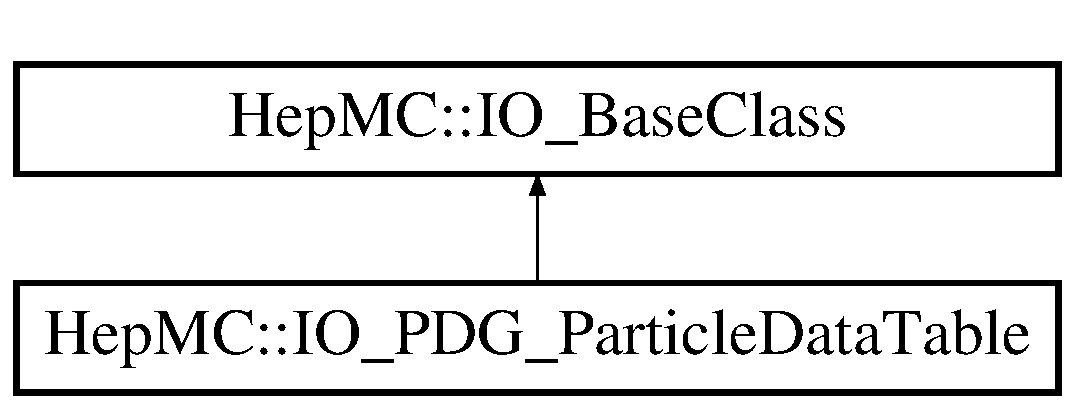
\includegraphics[height=2cm]{classHepMC_1_1IO__PDG__ParticleDataTable}
\end{center}
\end{figure}
\subsection*{Public Member Functions}
\begin{CompactItemize}
\item 
{\bf IO\_\-PDG\_\-Particle\-Data\-Table} (const char $\ast$filename=\char`\"{}PDG98\_\-Particle\-Data\-Table.txt\char`\"{})
\begin{CompactList}\small\item\em constructor using filename \item\end{CompactList}\item 
virtual {\bf $\sim$IO\_\-PDG\_\-Particle\-Data\-Table} ()
\item 
bool {\bf fill\_\-particle\_\-data\_\-table} ({\bf Particle\-Data\-Table} $\ast$)
\begin{CompactList}\small\item\em read the input and fill the table \item\end{CompactList}\item 
void {\bf add\_\-quarks\_\-to\_\-table} ({\bf Particle\-Data\-Table} \&)
\begin{CompactList}\small\item\em add u, d, s, c, b, and t \item\end{CompactList}\item 
void {\bf print} (std::ostream \&ostr=std::cout) const
\begin{CompactList}\small\item\em write to ostr \item\end{CompactList}\item 
int {\bf rdstate} () const
\begin{CompactList}\small\item\em check the IO state \item\end{CompactList}\end{CompactItemize}
\subsection*{Protected Member Functions}
\begin{CompactItemize}
\item 
bool {\bf search\_\-for\_\-key\_\-end} (std::istream \&in, const char $\ast$key)
\begin{CompactList}\small\item\em for internal use \item\end{CompactList}\item 
void {\bf read\_\-entry} ({\bf Particle\-Data\-Table} $\ast$)
\begin{CompactList}\small\item\em read a line \item\end{CompactList}\end{CompactItemize}


\subsection{Detailed Description}
an example \doxyref{Particle\-Data\-Table}{p.}{classHepMC_1_1ParticleDataTable} IO method 

Example of reading from file PDG98\_\-Particle\-Data\-Table.txt 



Definition at line 49 of file IO\_\-PDG\_\-Particle\-Data\-Table.h.

\subsection{Constructor \& Destructor Documentation}
\index{HepMC::IO_PDG_ParticleDataTable@{Hep\-MC::IO\_\-PDG\_\-Particle\-Data\-Table}!IO_PDG_ParticleDataTable@{IO\_\-PDG\_\-ParticleDataTable}}
\index{IO_PDG_ParticleDataTable@{IO\_\-PDG\_\-ParticleDataTable}!HepMC::IO_PDG_ParticleDataTable@{Hep\-MC::IO\_\-PDG\_\-Particle\-Data\-Table}}
\subsubsection{\setlength{\rightskip}{0pt plus 5cm}Hep\-MC::IO\_\-PDG\_\-Particle\-Data\-Table::IO\_\-PDG\_\-Particle\-Data\-Table (const char $\ast$ {\em filename} = {\tt \char`\"{}PDG98\_\-ParticleDataTable.txt\char`\"{}})}\label{classHepMC_1_1IO__PDG__ParticleDataTable_42b2879f7a5eb96515ba97e9f3699286}


constructor using filename 



Definition at line 17 of file IO\_\-PDG\_\-Particle\-Data\-Table.cc.\index{HepMC::IO_PDG_ParticleDataTable@{Hep\-MC::IO\_\-PDG\_\-Particle\-Data\-Table}!~IO_PDG_ParticleDataTable@{$\sim$IO\_\-PDG\_\-ParticleDataTable}}
\index{~IO_PDG_ParticleDataTable@{$\sim$IO\_\-PDG\_\-ParticleDataTable}!HepMC::IO_PDG_ParticleDataTable@{Hep\-MC::IO\_\-PDG\_\-Particle\-Data\-Table}}
\subsubsection{\setlength{\rightskip}{0pt plus 5cm}Hep\-MC::IO\_\-PDG\_\-Particle\-Data\-Table::$\sim$IO\_\-PDG\_\-Particle\-Data\-Table ()\hspace{0.3cm}{\tt  [virtual]}}\label{classHepMC_1_1IO__PDG__ParticleDataTable_ccd7a96ced82ebab0f554c26d5857fde}




Definition at line 20 of file IO\_\-PDG\_\-Particle\-Data\-Table.cc.

\subsection{Member Function Documentation}
\index{HepMC::IO_PDG_ParticleDataTable@{Hep\-MC::IO\_\-PDG\_\-Particle\-Data\-Table}!fill_particle_data_table@{fill\_\-particle\_\-data\_\-table}}
\index{fill_particle_data_table@{fill\_\-particle\_\-data\_\-table}!HepMC::IO_PDG_ParticleDataTable@{Hep\-MC::IO\_\-PDG\_\-Particle\-Data\-Table}}
\subsubsection{\setlength{\rightskip}{0pt plus 5cm}bool Hep\-MC::IO\_\-PDG\_\-Particle\-Data\-Table::fill\_\-particle\_\-data\_\-table ({\bf Particle\-Data\-Table} $\ast$)\hspace{0.3cm}{\tt  [virtual]}}\label{classHepMC_1_1IO__PDG__ParticleDataTable_6f0aee31fa762dfe83a686e4925adede}


read the input and fill the table 



Implements {\bf Hep\-MC::IO\_\-Base\-Class} \doxyref{}{p.}{classHepMC_1_1IO__BaseClass_094fc72dd621a2283989525497715feb}.

Definition at line 24 of file IO\_\-PDG\_\-Particle\-Data\-Table.cc.

References read\_\-entry(), search\_\-for\_\-key\_\-end(), and Hep\-MC::Particle\-Data\-Table::set\_\-description().\index{HepMC::IO_PDG_ParticleDataTable@{Hep\-MC::IO\_\-PDG\_\-Particle\-Data\-Table}!add_quarks_to_table@{add\_\-quarks\_\-to\_\-table}}
\index{add_quarks_to_table@{add\_\-quarks\_\-to\_\-table}!HepMC::IO_PDG_ParticleDataTable@{Hep\-MC::IO\_\-PDG\_\-Particle\-Data\-Table}}
\subsubsection{\setlength{\rightskip}{0pt plus 5cm}void Hep\-MC::IO\_\-PDG\_\-Particle\-Data\-Table::add\_\-quarks\_\-to\_\-table ({\bf Particle\-Data\-Table} \&)}\label{classHepMC_1_1IO__PDG__ParticleDataTable_9a745dbd5e599eaf27f5acec73c95caa}


add u, d, s, c, b, and t 



since quarks aren't included in PDG table, this method adds them 

Definition at line 165 of file IO\_\-PDG\_\-Particle\-Data\-Table.cc.

References Hep\-MC::Particle\-Data\-Table::erase(), Hep\-MC::Particle\-Data\-Table::find(), Hep\-MC::Particle\-Data\-Table::insert(), and Hep\-MC::Particle\-Data::mass().

Referenced by main().\index{HepMC::IO_PDG_ParticleDataTable@{Hep\-MC::IO\_\-PDG\_\-Particle\-Data\-Table}!print@{print}}
\index{print@{print}!HepMC::IO_PDG_ParticleDataTable@{Hep\-MC::IO\_\-PDG\_\-Particle\-Data\-Table}}
\subsubsection{\setlength{\rightskip}{0pt plus 5cm}void Hep\-MC::IO\_\-PDG\_\-Particle\-Data\-Table::print (std::ostream \& {\em ostr} = {\tt std::cout}) const\hspace{0.3cm}{\tt  [inline, virtual]}}\label{classHepMC_1_1IO__PDG__ParticleDataTable_3d125861cb0d1cafe6550e125111ff72}


write to ostr 



Reimplemented from {\bf Hep\-MC::IO\_\-Base\-Class} \doxyref{}{p.}{classHepMC_1_1IO__BaseClass_52a1503f4107fd3d5f4da02feb45751b}.

Definition at line 85 of file IO\_\-PDG\_\-Particle\-Data\-Table.h.\index{HepMC::IO_PDG_ParticleDataTable@{Hep\-MC::IO\_\-PDG\_\-Particle\-Data\-Table}!rdstate@{rdstate}}
\index{rdstate@{rdstate}!HepMC::IO_PDG_ParticleDataTable@{Hep\-MC::IO\_\-PDG\_\-Particle\-Data\-Table}}
\subsubsection{\setlength{\rightskip}{0pt plus 5cm}int Hep\-MC::IO\_\-PDG\_\-Particle\-Data\-Table::rdstate () const\hspace{0.3cm}{\tt  [inline]}}\label{classHepMC_1_1IO__PDG__ParticleDataTable_5165cc7ba14c3cf46f452b3c6760bbd3}


check the IO state 



Definition at line 63 of file IO\_\-PDG\_\-Particle\-Data\-Table.h.

Referenced by main().\index{HepMC::IO_PDG_ParticleDataTable@{Hep\-MC::IO\_\-PDG\_\-Particle\-Data\-Table}!search_for_key_end@{search\_\-for\_\-key\_\-end}}
\index{search_for_key_end@{search\_\-for\_\-key\_\-end}!HepMC::IO_PDG_ParticleDataTable@{Hep\-MC::IO\_\-PDG\_\-Particle\-Data\-Table}}
\subsubsection{\setlength{\rightskip}{0pt plus 5cm}bool Hep\-MC::IO\_\-PDG\_\-Particle\-Data\-Table::search\_\-for\_\-key\_\-end (std::istream \& {\em in}, const char $\ast$ {\em key})\hspace{0.3cm}{\tt  [protected]}}\label{classHepMC_1_1IO__PDG__ParticleDataTable_18660746b1be0c4c7645be91e5749141}


for internal use 



(this method borrowed from \doxyref{IO\_\-Ascii}{p.}{classHepMC_1_1IO__Ascii} class) reads characters from in until the string of characters matching key is found (success) or EOF is reached (failure). It stops immediately thereafter. Returns T/F for success/fail 

Definition at line 203 of file IO\_\-PDG\_\-Particle\-Data\-Table.cc.

Referenced by fill\_\-particle\_\-data\_\-table().\index{HepMC::IO_PDG_ParticleDataTable@{Hep\-MC::IO\_\-PDG\_\-Particle\-Data\-Table}!read_entry@{read\_\-entry}}
\index{read_entry@{read\_\-entry}!HepMC::IO_PDG_ParticleDataTable@{Hep\-MC::IO\_\-PDG\_\-Particle\-Data\-Table}}
\subsubsection{\setlength{\rightskip}{0pt plus 5cm}void Hep\-MC::IO\_\-PDG\_\-Particle\-Data\-Table::read\_\-entry ({\bf Particle\-Data\-Table} $\ast$)\hspace{0.3cm}{\tt  [protected]}}\label{classHepMC_1_1IO__PDG__ParticleDataTable_1edcdadccf0ec361acd2c926468dc2a4}


read a line 



Definition at line 63 of file IO\_\-PDG\_\-Particle\-Data\-Table.cc.

References Hep\-MC::clifetime\_\-from\_\-width(), Hep\-MC::Particle\-Data\-Table::find(), Hep\-MC::Particle\-Data\-Table::insert(), Hep\-MC::Particle\-Data::set\_\-clifetime(), and Hep\-MC::Particle\-Data::set\_\-mass().

Referenced by fill\_\-particle\_\-data\_\-table().

The documentation for this class was generated from the following files:\begin{CompactItemize}
\item 
{\bf IO\_\-PDG\_\-Particle\-Data\-Table.h}\item 
{\bf IO\_\-PDG\_\-Particle\-Data\-Table.cc}\end{CompactItemize}

\section{Hep\-MC::detail::is\_\-arithmetic$<$ T $>$ Struct Template Reference}
\label{structHepMC_1_1detail_1_1is__arithmetic}\index{HepMC::detail::is_arithmetic@{HepMC::detail::is\_\-arithmetic}}
undefined and therefore non-arithmetic  


{\tt \#include $<$is\_\-arithmetic.h$>$}

\subsection*{Static Public Attributes}
\begin{CompactItemize}
\item 
static bool const {\bf value} = false
\end{CompactItemize}


\subsection{Detailed Description}
\subsubsection*{template$<$class T$>$ struct Hep\-MC::detail::is\_\-arithmetic$<$ T $>$}

undefined and therefore non-arithmetic 



Definition at line 22 of file is\_\-arithmetic.h.

\subsection{Member Data Documentation}
\index{HepMC::detail::is_arithmetic@{Hep\-MC::detail::is\_\-arithmetic}!value@{value}}
\index{value@{value}!HepMC::detail::is_arithmetic@{Hep\-MC::detail::is\_\-arithmetic}}
\subsubsection{\setlength{\rightskip}{0pt plus 5cm}template$<$class T$>$ bool const {\bf Hep\-MC::detail::is\_\-arithmetic}$<$ T $>$::{\bf value} = false\hspace{0.3cm}{\tt  [static]}}\label{structHepMC_1_1detail_1_1is__arithmetic_10629487031fd5e2212737df84dafe56}




Definition at line 24 of file is\_\-arithmetic.h.

The documentation for this struct was generated from the following file:\begin{CompactItemize}
\item 
{\bf is\_\-arithmetic.h}\end{CompactItemize}

\section{Hep\-MC::detail::is\_\-arithmetic$<$ char $>$ Struct Template Reference}
\label{structHepMC_1_1detail_1_1is__arithmetic_3_01char_01_4}\index{HepMC::detail::is_arithmetic< char >@{HepMC::detail::is\_\-arithmetic$<$ char $>$}}
character is arithmetic  


{\tt \#include $<$is\_\-arithmetic.h$>$}

\subsection*{Static Public Attributes}
\begin{CompactItemize}
\item 
static bool const {\bf value} = true
\end{CompactItemize}


\subsection{Detailed Description}
\subsubsection*{template$<$$>$ struct Hep\-MC::detail::is\_\-arithmetic$<$ char $>$}

character is arithmetic 



Definition at line 29 of file is\_\-arithmetic.h.

\subsection{Member Data Documentation}
\index{HepMC::detail::is_arithmetic< char >@{Hep\-MC::detail::is\_\-arithmetic$<$ char $>$}!value@{value}}
\index{value@{value}!HepMC::detail::is_arithmetic< char >@{Hep\-MC::detail::is\_\-arithmetic$<$ char $>$}}
\subsubsection{\setlength{\rightskip}{0pt plus 5cm}bool const {\bf Hep\-MC::detail::is\_\-arithmetic}$<$ char $>$::{\bf value} = true\hspace{0.3cm}{\tt  [static]}}\label{structHepMC_1_1detail_1_1is__arithmetic_3_01char_01_4_5fb6287c231568d405d97bb739395d33}




Definition at line 30 of file is\_\-arithmetic.h.

The documentation for this struct was generated from the following file:\begin{CompactItemize}
\item 
{\bf is\_\-arithmetic.h}\end{CompactItemize}

\section{Hep\-MC::detail::is\_\-arithmetic$<$ double $>$ Struct Template Reference}
\label{structHepMC_1_1detail_1_1is__arithmetic_3_01double_01_4}\index{HepMC::detail::is_arithmetic< double >@{HepMC::detail::is\_\-arithmetic$<$ double $>$}}
double is arithmetic  


{\tt \#include $<$is\_\-arithmetic.h$>$}

\subsection*{Static Public Attributes}
\begin{CompactItemize}
\item 
static bool const {\bf value} = true
\end{CompactItemize}


\subsection{Detailed Description}
\subsubsection*{template$<$$>$ struct Hep\-MC::detail::is\_\-arithmetic$<$ double $>$}

double is arithmetic 



Definition at line 79 of file is\_\-arithmetic.h.

\subsection{Member Data Documentation}
\index{HepMC::detail::is_arithmetic< double >@{Hep\-MC::detail::is\_\-arithmetic$<$ double $>$}!value@{value}}
\index{value@{value}!HepMC::detail::is_arithmetic< double >@{Hep\-MC::detail::is\_\-arithmetic$<$ double $>$}}
\subsubsection{\setlength{\rightskip}{0pt plus 5cm}bool const {\bf Hep\-MC::detail::is\_\-arithmetic}$<$ double $>$::{\bf value} = true\hspace{0.3cm}{\tt  [static]}}\label{structHepMC_1_1detail_1_1is__arithmetic_3_01double_01_4_a795bfdda0c19f00643eedc84f3b0fe0}




Definition at line 80 of file is\_\-arithmetic.h.

The documentation for this struct was generated from the following file:\begin{CompactItemize}
\item 
{\bf is\_\-arithmetic.h}\end{CompactItemize}

\section{Hep\-MC::detail::is\_\-arithmetic$<$ float $>$ Struct Template Reference}
\label{structHepMC_1_1detail_1_1is__arithmetic_3_01float_01_4}\index{HepMC::detail::is_arithmetic< float >@{HepMC::detail::is\_\-arithmetic$<$ float $>$}}
float is arithmetic  


{\tt \#include $<$is\_\-arithmetic.h$>$}

\subsection*{Static Public Attributes}
\begin{CompactItemize}
\item 
static bool const {\bf value} = true
\end{CompactItemize}


\subsection{Detailed Description}
\subsubsection*{template$<$$>$ struct Hep\-MC::detail::is\_\-arithmetic$<$ float $>$}

float is arithmetic 



Definition at line 74 of file is\_\-arithmetic.h.

\subsection{Member Data Documentation}
\index{HepMC::detail::is_arithmetic< float >@{Hep\-MC::detail::is\_\-arithmetic$<$ float $>$}!value@{value}}
\index{value@{value}!HepMC::detail::is_arithmetic< float >@{Hep\-MC::detail::is\_\-arithmetic$<$ float $>$}}
\subsubsection{\setlength{\rightskip}{0pt plus 5cm}bool const {\bf Hep\-MC::detail::is\_\-arithmetic}$<$ float $>$::{\bf value} = true\hspace{0.3cm}{\tt  [static]}}\label{structHepMC_1_1detail_1_1is__arithmetic_3_01float_01_4_ead3df450e02b59ea9cda6b63728adbe}




Definition at line 75 of file is\_\-arithmetic.h.

The documentation for this struct was generated from the following file:\begin{CompactItemize}
\item 
{\bf is\_\-arithmetic.h}\end{CompactItemize}

\section{Hep\-MC::detail::is\_\-arithmetic$<$ int $>$ Struct Template Reference}
\label{structHepMC_1_1detail_1_1is__arithmetic_3_01int_01_4}\index{HepMC::detail::is_arithmetic< int >@{HepMC::detail::is\_\-arithmetic$<$ int $>$}}
int is arithmetic  


{\tt \#include $<$is\_\-arithmetic.h$>$}

\subsection*{Static Public Attributes}
\begin{CompactItemize}
\item 
static bool const {\bf value} = true
\end{CompactItemize}


\subsection{Detailed Description}
\subsubsection*{template$<$$>$ struct Hep\-MC::detail::is\_\-arithmetic$<$ int $>$}

int is arithmetic 



Definition at line 54 of file is\_\-arithmetic.h.

\subsection{Member Data Documentation}
\index{HepMC::detail::is_arithmetic< int >@{Hep\-MC::detail::is\_\-arithmetic$<$ int $>$}!value@{value}}
\index{value@{value}!HepMC::detail::is_arithmetic< int >@{Hep\-MC::detail::is\_\-arithmetic$<$ int $>$}}
\subsubsection{\setlength{\rightskip}{0pt plus 5cm}bool const {\bf Hep\-MC::detail::is\_\-arithmetic}$<$ int $>$::{\bf value} = true\hspace{0.3cm}{\tt  [static]}}\label{structHepMC_1_1detail_1_1is__arithmetic_3_01int_01_4_c851518d895c0f7d7b834aa2b6deb388}




Definition at line 55 of file is\_\-arithmetic.h.

The documentation for this struct was generated from the following file:\begin{CompactItemize}
\item 
{\bf is\_\-arithmetic.h}\end{CompactItemize}

\section{Hep\-MC::detail::is\_\-arithmetic$<$ long $>$ Struct Template Reference}
\label{structHepMC_1_1detail_1_1is__arithmetic_3_01long_01_4}\index{HepMC::detail::is_arithmetic< long >@{HepMC::detail::is\_\-arithmetic$<$ long $>$}}
long is arithmetic  


{\tt \#include $<$is\_\-arithmetic.h$>$}

\subsection*{Static Public Attributes}
\begin{CompactItemize}
\item 
static bool const {\bf value} = true
\end{CompactItemize}


\subsection{Detailed Description}
\subsubsection*{template$<$$>$ struct Hep\-MC::detail::is\_\-arithmetic$<$ long $>$}

long is arithmetic 



Definition at line 64 of file is\_\-arithmetic.h.

\subsection{Member Data Documentation}
\index{HepMC::detail::is_arithmetic< long >@{Hep\-MC::detail::is\_\-arithmetic$<$ long $>$}!value@{value}}
\index{value@{value}!HepMC::detail::is_arithmetic< long >@{Hep\-MC::detail::is\_\-arithmetic$<$ long $>$}}
\subsubsection{\setlength{\rightskip}{0pt plus 5cm}bool const {\bf Hep\-MC::detail::is\_\-arithmetic}$<$ long $>$::{\bf value} = true\hspace{0.3cm}{\tt  [static]}}\label{structHepMC_1_1detail_1_1is__arithmetic_3_01long_01_4_e0d773a0ff3d52d407b8306f0e1c67f0}




Definition at line 65 of file is\_\-arithmetic.h.

The documentation for this struct was generated from the following file:\begin{CompactItemize}
\item 
{\bf is\_\-arithmetic.h}\end{CompactItemize}

\section{Hep\-MC::detail::is\_\-arithmetic$<$ long double $>$ Struct Template Reference}
\label{structHepMC_1_1detail_1_1is__arithmetic_3_01long_01double_01_4}\index{HepMC::detail::is_arithmetic< long double >@{HepMC::detail::is\_\-arithmetic$<$ long double $>$}}
long double is arithmetic  


{\tt \#include $<$is\_\-arithmetic.h$>$}

\subsection*{Static Public Attributes}
\begin{CompactItemize}
\item 
static bool const {\bf value} = true
\end{CompactItemize}


\subsection{Detailed Description}
\subsubsection*{template$<$$>$ struct Hep\-MC::detail::is\_\-arithmetic$<$ long double $>$}

long double is arithmetic 



Definition at line 84 of file is\_\-arithmetic.h.

\subsection{Member Data Documentation}
\index{HepMC::detail::is_arithmetic< long double >@{Hep\-MC::detail::is\_\-arithmetic$<$ long double $>$}!value@{value}}
\index{value@{value}!HepMC::detail::is_arithmetic< long double >@{Hep\-MC::detail::is\_\-arithmetic$<$ long double $>$}}
\subsubsection{\setlength{\rightskip}{0pt plus 5cm}bool const {\bf Hep\-MC::detail::is\_\-arithmetic}$<$ long double $>$::{\bf value} = true\hspace{0.3cm}{\tt  [static]}}\label{structHepMC_1_1detail_1_1is__arithmetic_3_01long_01double_01_4_1f2633b86bf19138dba60a5090860b71}




Definition at line 85 of file is\_\-arithmetic.h.

The documentation for this struct was generated from the following file:\begin{CompactItemize}
\item 
{\bf is\_\-arithmetic.h}\end{CompactItemize}

\section{Hep\-MC::detail::is\_\-arithmetic$<$ short $>$ Struct Template Reference}
\label{structHepMC_1_1detail_1_1is__arithmetic_3_01short_01_4}\index{HepMC::detail::is_arithmetic< short >@{HepMC::detail::is\_\-arithmetic$<$ short $>$}}
short is arithmetic  


{\tt \#include $<$is\_\-arithmetic.h$>$}

\subsection*{Static Public Attributes}
\begin{CompactItemize}
\item 
static bool const {\bf value} = true
\end{CompactItemize}


\subsection{Detailed Description}
\subsubsection*{template$<$$>$ struct Hep\-MC::detail::is\_\-arithmetic$<$ short $>$}

short is arithmetic 



Definition at line 44 of file is\_\-arithmetic.h.

\subsection{Member Data Documentation}
\index{HepMC::detail::is_arithmetic< short >@{Hep\-MC::detail::is\_\-arithmetic$<$ short $>$}!value@{value}}
\index{value@{value}!HepMC::detail::is_arithmetic< short >@{Hep\-MC::detail::is\_\-arithmetic$<$ short $>$}}
\subsubsection{\setlength{\rightskip}{0pt plus 5cm}bool const {\bf Hep\-MC::detail::is\_\-arithmetic}$<$ short $>$::{\bf value} = true\hspace{0.3cm}{\tt  [static]}}\label{structHepMC_1_1detail_1_1is__arithmetic_3_01short_01_4_23a7af930b496eaae0024ca759cc7e09}




Definition at line 45 of file is\_\-arithmetic.h.

The documentation for this struct was generated from the following file:\begin{CompactItemize}
\item 
{\bf is\_\-arithmetic.h}\end{CompactItemize}

\section{Hep\-MC::detail::is\_\-arithmetic$<$ signed char $>$ Struct Template Reference}
\label{structHepMC_1_1detail_1_1is__arithmetic_3_01signed_01char_01_4}\index{HepMC::detail::is_arithmetic< signed char >@{HepMC::detail::is\_\-arithmetic$<$ signed char $>$}}
signed character is arithmetic  


{\tt \#include $<$is\_\-arithmetic.h$>$}

\subsection*{Static Public Attributes}
\begin{CompactItemize}
\item 
static bool const {\bf value} = true
\end{CompactItemize}


\subsection{Detailed Description}
\subsubsection*{template$<$$>$ struct Hep\-MC::detail::is\_\-arithmetic$<$ signed char $>$}

signed character is arithmetic 



Definition at line 39 of file is\_\-arithmetic.h.

\subsection{Member Data Documentation}
\index{HepMC::detail::is_arithmetic< signed char >@{Hep\-MC::detail::is\_\-arithmetic$<$ signed char $>$}!value@{value}}
\index{value@{value}!HepMC::detail::is_arithmetic< signed char >@{Hep\-MC::detail::is\_\-arithmetic$<$ signed char $>$}}
\subsubsection{\setlength{\rightskip}{0pt plus 5cm}bool const {\bf Hep\-MC::detail::is\_\-arithmetic}$<$ signed char $>$::{\bf value} = true\hspace{0.3cm}{\tt  [static]}}\label{structHepMC_1_1detail_1_1is__arithmetic_3_01signed_01char_01_4_724a5b700a3422dfdd35673e9e23d3ea}




Definition at line 40 of file is\_\-arithmetic.h.

The documentation for this struct was generated from the following file:\begin{CompactItemize}
\item 
{\bf is\_\-arithmetic.h}\end{CompactItemize}

\section{Hep\-MC::detail::is\_\-arithmetic$<$ unsigned char $>$ Struct Template Reference}
\label{structHepMC_1_1detail_1_1is__arithmetic_3_01unsigned_01char_01_4}\index{HepMC::detail::is_arithmetic< unsigned char >@{HepMC::detail::is\_\-arithmetic$<$ unsigned char $>$}}
unsigned character is arithmetic  


{\tt \#include $<$is\_\-arithmetic.h$>$}

\subsection*{Static Public Attributes}
\begin{CompactItemize}
\item 
static bool const {\bf value} = true
\end{CompactItemize}


\subsection{Detailed Description}
\subsubsection*{template$<$$>$ struct Hep\-MC::detail::is\_\-arithmetic$<$ unsigned char $>$}

unsigned character is arithmetic 



Definition at line 34 of file is\_\-arithmetic.h.

\subsection{Member Data Documentation}
\index{HepMC::detail::is_arithmetic< unsigned char >@{Hep\-MC::detail::is\_\-arithmetic$<$ unsigned char $>$}!value@{value}}
\index{value@{value}!HepMC::detail::is_arithmetic< unsigned char >@{Hep\-MC::detail::is\_\-arithmetic$<$ unsigned char $>$}}
\subsubsection{\setlength{\rightskip}{0pt plus 5cm}bool const {\bf Hep\-MC::detail::is\_\-arithmetic}$<$ unsigned char $>$::{\bf value} = true\hspace{0.3cm}{\tt  [static]}}\label{structHepMC_1_1detail_1_1is__arithmetic_3_01unsigned_01char_01_4_f0a8652f44c6b389fadd385f9e373c05}




Definition at line 35 of file is\_\-arithmetic.h.

The documentation for this struct was generated from the following file:\begin{CompactItemize}
\item 
{\bf is\_\-arithmetic.h}\end{CompactItemize}

\section{Hep\-MC::detail::is\_\-arithmetic$<$ unsigned int $>$ Struct Template Reference}
\label{structHepMC_1_1detail_1_1is__arithmetic_3_01unsigned_01int_01_4}\index{HepMC::detail::is_arithmetic< unsigned int >@{HepMC::detail::is\_\-arithmetic$<$ unsigned int $>$}}
unsigned int is arithmetic  


{\tt \#include $<$is\_\-arithmetic.h$>$}

\subsection*{Static Public Attributes}
\begin{CompactItemize}
\item 
static bool const {\bf value} = true
\end{CompactItemize}


\subsection{Detailed Description}
\subsubsection*{template$<$$>$ struct Hep\-MC::detail::is\_\-arithmetic$<$ unsigned int $>$}

unsigned int is arithmetic 



Definition at line 59 of file is\_\-arithmetic.h.

\subsection{Member Data Documentation}
\index{HepMC::detail::is_arithmetic< unsigned int >@{Hep\-MC::detail::is\_\-arithmetic$<$ unsigned int $>$}!value@{value}}
\index{value@{value}!HepMC::detail::is_arithmetic< unsigned int >@{Hep\-MC::detail::is\_\-arithmetic$<$ unsigned int $>$}}
\subsubsection{\setlength{\rightskip}{0pt plus 5cm}bool const {\bf Hep\-MC::detail::is\_\-arithmetic}$<$ unsigned int $>$::{\bf value} = true\hspace{0.3cm}{\tt  [static]}}\label{structHepMC_1_1detail_1_1is__arithmetic_3_01unsigned_01int_01_4_613695c9983cc5e22db670398434928a}




Definition at line 60 of file is\_\-arithmetic.h.

The documentation for this struct was generated from the following file:\begin{CompactItemize}
\item 
{\bf is\_\-arithmetic.h}\end{CompactItemize}

\section{Hep\-MC::detail::is\_\-arithmetic$<$ unsigned long $>$ Struct Template Reference}
\label{structHepMC_1_1detail_1_1is__arithmetic_3_01unsigned_01long_01_4}\index{HepMC::detail::is_arithmetic< unsigned long >@{HepMC::detail::is\_\-arithmetic$<$ unsigned long $>$}}
unsigned long is arithmetic  


{\tt \#include $<$is\_\-arithmetic.h$>$}

\subsection*{Static Public Attributes}
\begin{CompactItemize}
\item 
static bool const {\bf value} = true
\end{CompactItemize}


\subsection{Detailed Description}
\subsubsection*{template$<$$>$ struct Hep\-MC::detail::is\_\-arithmetic$<$ unsigned long $>$}

unsigned long is arithmetic 



Definition at line 69 of file is\_\-arithmetic.h.

\subsection{Member Data Documentation}
\index{HepMC::detail::is_arithmetic< unsigned long >@{Hep\-MC::detail::is\_\-arithmetic$<$ unsigned long $>$}!value@{value}}
\index{value@{value}!HepMC::detail::is_arithmetic< unsigned long >@{Hep\-MC::detail::is\_\-arithmetic$<$ unsigned long $>$}}
\subsubsection{\setlength{\rightskip}{0pt plus 5cm}bool const {\bf Hep\-MC::detail::is\_\-arithmetic}$<$ unsigned long $>$::{\bf value} = true\hspace{0.3cm}{\tt  [static]}}\label{structHepMC_1_1detail_1_1is__arithmetic_3_01unsigned_01long_01_4_5337746dfc4a8b11f18c764aafca52b4}




Definition at line 70 of file is\_\-arithmetic.h.

The documentation for this struct was generated from the following file:\begin{CompactItemize}
\item 
{\bf is\_\-arithmetic.h}\end{CompactItemize}

\section{Hep\-MC::detail::is\_\-arithmetic$<$ unsigned short $>$ Struct Template Reference}
\label{structHepMC_1_1detail_1_1is__arithmetic_3_01unsigned_01short_01_4}\index{HepMC::detail::is_arithmetic< unsigned short >@{HepMC::detail::is\_\-arithmetic$<$ unsigned short $>$}}
unsigned short is arithmetic  


{\tt \#include $<$is\_\-arithmetic.h$>$}

\subsection*{Static Public Attributes}
\begin{CompactItemize}
\item 
static bool const {\bf value} = true
\end{CompactItemize}


\subsection{Detailed Description}
\subsubsection*{template$<$$>$ struct Hep\-MC::detail::is\_\-arithmetic$<$ unsigned short $>$}

unsigned short is arithmetic 



Definition at line 49 of file is\_\-arithmetic.h.

\subsection{Member Data Documentation}
\index{HepMC::detail::is_arithmetic< unsigned short >@{Hep\-MC::detail::is\_\-arithmetic$<$ unsigned short $>$}!value@{value}}
\index{value@{value}!HepMC::detail::is_arithmetic< unsigned short >@{Hep\-MC::detail::is\_\-arithmetic$<$ unsigned short $>$}}
\subsubsection{\setlength{\rightskip}{0pt plus 5cm}bool const {\bf Hep\-MC::detail::is\_\-arithmetic}$<$ unsigned short $>$::{\bf value} = true\hspace{0.3cm}{\tt  [static]}}\label{structHepMC_1_1detail_1_1is__arithmetic_3_01unsigned_01short_01_4_04eeb23cc6ce29893eabd8be90ee69d3}




Definition at line 50 of file is\_\-arithmetic.h.

The documentation for this struct was generated from the following file:\begin{CompactItemize}
\item 
{\bf is\_\-arithmetic.h}\end{CompactItemize}

\section{Is\-Final\-State Class Reference}
\label{classIsFinalState}\index{IsFinalState@{IsFinalState}}
example class  


{\tt \#include $<$test\-Hep\-MCIteration.h$>$}

\subsection*{Public Member Functions}
\begin{CompactItemize}
\item 
bool {\bf operator()} (const {\bf Hep\-MC::Gen\-Particle} $\ast${\bf p})
\begin{CompactList}\small\item\em returns true if the Gen\-Particle does not decay \item\end{CompactList}\item 
bool {\bf operator()} (const {\bf Hep\-MC::Gen\-Particle} $\ast${\bf p})
\begin{CompactList}\small\item\em returns true if the Gen\-Particle does not decay \item\end{CompactList}\end{CompactItemize}


\subsection{Detailed Description}
example class 

this predicate returns true if the input has no decay vertex \begin{Desc}
\item[Examples: ]\par


{\bf example\_\-Using\-Iterators.cc}.\end{Desc}




Definition at line 47 of file example\_\-Using\-Iterators.cc.

\subsection{Member Function Documentation}
\index{IsFinalState@{Is\-Final\-State}!operator()@{operator()}}
\index{operator()@{operator()}!IsFinalState@{Is\-Final\-State}}
\subsubsection{\setlength{\rightskip}{0pt plus 5cm}bool Is\-Final\-State::operator() (const {\bf Hep\-MC::Gen\-Particle} $\ast$ {\em p})\hspace{0.3cm}{\tt  [inline]}}\label{classIsFinalState_62aeba27a39989c7bbccef8a0fa7626a}


returns true if the Gen\-Particle does not decay 

\begin{Desc}
\item[Examples: ]\par
{\bf example\_\-Using\-Iterators.cc}.\end{Desc}


Definition at line 50 of file example\_\-Using\-Iterators.cc.

References p.\index{IsFinalState@{Is\-Final\-State}!operator()@{operator()}}
\index{operator()@{operator()}!IsFinalState@{Is\-Final\-State}}
\subsubsection{\setlength{\rightskip}{0pt plus 5cm}bool Is\-Final\-State::operator() (const {\bf Hep\-MC::Gen\-Particle} $\ast$ {\em p})\hspace{0.3cm}{\tt  [inline]}}\label{classIsFinalState_62aeba27a39989c7bbccef8a0fa7626a}


returns true if the Gen\-Particle does not decay 



Definition at line 29 of file test\-Hep\-MCIteration.h.

References p.

The documentation for this class was generated from the following files:\begin{CompactItemize}
\item 
{\bf example\_\-Using\-Iterators.cc}\item 
{\bf test\-Hep\-MCIteration.h}\end{CompactItemize}

\section{Is\-Good\-Event Class Reference}
\label{classIsGoodEvent}\index{IsGoodEvent@{IsGoodEvent}}
example class  


{\tt \#include $<$Is\-Good\-Event.h$>$}

\subsection*{Public Member Functions}
\begin{CompactItemize}
\item 
bool {\bf operator()} (const {\bf Hep\-MC::Gen\-Event} $\ast$evt)
\begin{CompactList}\small\item\em check this event for goodness \item\end{CompactList}\item 
bool {\bf operator()} (const {\bf Hep\-MC::Gen\-Event} $\ast$evt)
\end{CompactItemize}


\subsection{Detailed Description}
example class 

event selection predicate. returns true if the event contains a photon with p\-T $>$ 50 Ge\-V \begin{Desc}
\item[Examples: ]\par


{\bf example\_\-Event\-Selection.cc}.\end{Desc}




Definition at line 20 of file example\_\-Event\-Selection.cc.

\subsection{Member Function Documentation}
\index{IsGoodEvent@{Is\-Good\-Event}!operator()@{operator()}}
\index{operator()@{operator()}!IsGoodEvent@{Is\-Good\-Event}}
\subsubsection{\setlength{\rightskip}{0pt plus 5cm}bool Is\-Good\-Event::operator() (const {\bf Hep\-MC::Gen\-Event} $\ast$ {\em evt})\hspace{0.3cm}{\tt  [inline]}}\label{classIsGoodEvent_eb8864821e4db5babf9b002764a8b295}


check this event for goodness 

\begin{Desc}
\item[Examples: ]\par
{\bf example\_\-Event\-Selection.cc}.\end{Desc}


Definition at line 23 of file example\_\-Event\-Selection.cc.

References p, Hep\-MC::Gen\-Event::particles\_\-begin(), and Hep\-MC::Gen\-Event::particles\_\-end().\index{IsGoodEvent@{Is\-Good\-Event}!operator()@{operator()}}
\index{operator()@{operator()}!IsGoodEvent@{Is\-Good\-Event}}
\subsubsection{\setlength{\rightskip}{0pt plus 5cm}bool Is\-Good\-Event::operator() (const {\bf Hep\-MC::Gen\-Event} $\ast$ {\em evt})\hspace{0.3cm}{\tt  [inline]}}\label{classIsGoodEvent_eb8864821e4db5babf9b002764a8b295}




Definition at line 14 of file Is\-Good\-Event.h.

References p, Hep\-MC::Gen\-Event::particles\_\-begin(), and Hep\-MC::Gen\-Event::particles\_\-end().

The documentation for this class was generated from the following files:\begin{CompactItemize}
\item 
{\bf example\_\-Event\-Selection.cc}\item 
{\bf Is\-Good\-Event.h}\end{CompactItemize}

\section{Is\-Good\-Event\-My\-Pythia Class Reference}
\label{classIsGoodEventMyPythia}\index{IsGoodEventMyPythia@{IsGoodEventMyPythia}}
example class  


\subsection*{Public Member Functions}
\begin{CompactItemize}
\item 
bool {\bf operator()} (const {\bf Hep\-MC::Gen\-Event} $\ast$evt)
\begin{CompactList}\small\item\em returns true if event is \char`\"{}good\char`\"{} \item\end{CompactList}\end{CompactItemize}


\subsection{Detailed Description}
example class 

event selection predicate. returns true if the event contains a photon with p\-T $>$ 25 Ge\-V \begin{Desc}
\item[Examples: ]\par


{\bf example\_\-My\-Pythia\-With\-Event\-Selection.cc}.\end{Desc}




Definition at line 28 of file example\_\-My\-Pythia\-With\-Event\-Selection.cc.

\subsection{Member Function Documentation}
\index{IsGoodEventMyPythia@{Is\-Good\-Event\-My\-Pythia}!operator()@{operator()}}
\index{operator()@{operator()}!IsGoodEventMyPythia@{Is\-Good\-Event\-My\-Pythia}}
\subsubsection{\setlength{\rightskip}{0pt plus 5cm}bool Is\-Good\-Event\-My\-Pythia::operator() (const {\bf Hep\-MC::Gen\-Event} $\ast$ {\em evt})\hspace{0.3cm}{\tt  [inline]}}\label{classIsGoodEventMyPythia_d9cc41932485930274176d8d0d4171d1}


returns true if event is \char`\"{}good\char`\"{} 

\begin{Desc}
\item[Examples: ]\par
{\bf example\_\-My\-Pythia\-With\-Event\-Selection.cc}.\end{Desc}


Definition at line 31 of file example\_\-My\-Pythia\-With\-Event\-Selection.cc.

References p, Hep\-MC::Gen\-Event::particles\_\-begin(), and Hep\-MC::Gen\-Event::particles\_\-end().

The documentation for this class was generated from the following file:\begin{CompactItemize}
\item 
{\bf example\_\-My\-Pythia\-With\-Event\-Selection.cc}\end{CompactItemize}

\section{Is\-Photon Class Reference}
\label{classIsPhoton}\index{IsPhoton@{IsPhoton}}
example class  


\subsection*{Public Member Functions}
\begin{CompactItemize}
\item 
bool {\bf operator()} (const {\bf Hep\-MC::Gen\-Particle} $\ast${\bf p})
\begin{CompactList}\small\item\em returns true if the Gen\-Particle is a photon with more than 10 Ge\-V transverse momentum \item\end{CompactList}\end{CompactItemize}


\subsection{Detailed Description}
example class 

this predicate returns true if the input particle is a photon in the central region (eta $<$ 2.5) with p\-T $>$ 10 Ge\-V \begin{Desc}
\item[Examples: ]\par


{\bf example\_\-Using\-Iterators.cc}.\end{Desc}




Definition at line 20 of file example\_\-Using\-Iterators.cc.

\subsection{Member Function Documentation}
\index{IsPhoton@{Is\-Photon}!operator()@{operator()}}
\index{operator()@{operator()}!IsPhoton@{Is\-Photon}}
\subsubsection{\setlength{\rightskip}{0pt plus 5cm}bool Is\-Photon::operator() (const {\bf Hep\-MC::Gen\-Particle} $\ast$ {\em p})\hspace{0.3cm}{\tt  [inline]}}\label{classIsPhoton_8ed40aa03fd51c1639078f75a0902f98}


returns true if the Gen\-Particle is a photon with more than 10 Ge\-V transverse momentum 

\begin{Desc}
\item[Examples: ]\par
{\bf example\_\-Using\-Iterators.cc}.\end{Desc}


Definition at line 23 of file example\_\-Using\-Iterators.cc.

References p.

The documentation for this class was generated from the following file:\begin{CompactItemize}
\item 
{\bf example\_\-Using\-Iterators.cc}\end{CompactItemize}

\section{Is\-W\_\-Boson Class Reference}
\label{classIsW__Boson}\index{IsW_Boson@{IsW\_\-Boson}}
example class  


\subsection*{Public Member Functions}
\begin{CompactItemize}
\item 
bool {\bf operator()} (const {\bf Hep\-MC::Gen\-Particle} $\ast${\bf p})
\begin{CompactList}\small\item\em returns true if the Gen\-Particle is a W \item\end{CompactList}\end{CompactItemize}


\subsection{Detailed Description}
example class 

this predicate returns true if the input particle is a W+/W- \begin{Desc}
\item[Examples: ]\par


{\bf example\_\-Using\-Iterators.cc}.\end{Desc}




Definition at line 34 of file example\_\-Using\-Iterators.cc.

\subsection{Member Function Documentation}
\index{IsW_Boson@{Is\-W\_\-Boson}!operator()@{operator()}}
\index{operator()@{operator()}!IsW_Boson@{Is\-W\_\-Boson}}
\subsubsection{\setlength{\rightskip}{0pt plus 5cm}bool Is\-W\_\-Boson::operator() (const {\bf Hep\-MC::Gen\-Particle} $\ast$ {\em p})\hspace{0.3cm}{\tt  [inline]}}\label{classIsW__Boson_206d7b0078c631b69c2cbc4c81846e55}


returns true if the Gen\-Particle is a W 

\begin{Desc}
\item[Examples: ]\par
{\bf example\_\-Using\-Iterators.cc}.\end{Desc}


Definition at line 37 of file example\_\-Using\-Iterators.cc.

References p.

The documentation for this class was generated from the following file:\begin{CompactItemize}
\item 
{\bf example\_\-Using\-Iterators.cc}\end{CompactItemize}

\section{Hep\-MC::Particle\-Data Class Reference}
\label{classHepMC_1_1ParticleData}\index{HepMC::ParticleData@{HepMC::ParticleData}}
an example \doxyref{Particle\-Data}{p.}{classHepMC_1_1ParticleData} class  


{\tt \#include $<$Particle\-Data.h$>$}

\subsection*{Public Member Functions}
\begin{CompactItemize}
\item 
{\bf Particle\-Data} (std::string name, int id, double charge, double mass=0, double c\-Lifetime=-1, double spin=0)
\begin{CompactList}\small\item\em constructor requiring name, ID, and charge \item\end{CompactList}\item 
{\bf Particle\-Data} (const char $\ast$name, int id, double charge, double mass=0, double c\-Lifetime=-1, double spin=0)
\begin{CompactList}\small\item\em constructor requiring name, ID, and charge \item\end{CompactList}\item 
virtual {\bf $\sim$Particle\-Data} ()
\item 
bool {\bf operator==} (const {\bf Particle\-Data} \&) const
\begin{CompactList}\small\item\em equality \item\end{CompactList}\item 
bool {\bf operator!=} (const {\bf Particle\-Data} \&) const
\begin{CompactList}\small\item\em inequality \item\end{CompactList}\item 
void {\bf print} (std::ostream \&ostr=std::cout) const
\begin{CompactList}\small\item\em write particle data information to ostr \item\end{CompactList}\item 
bool {\bf is\_\-lepton} () const
\begin{CompactList}\small\item\em true if charged lepton /neutrino \item\end{CompactList}\item 
bool {\bf is\_\-charged\_\-lepton} () const
\begin{CompactList}\small\item\em true if a charged lepton \item\end{CompactList}\item 
bool {\bf is\_\-em} () const
\begin{CompactList}\small\item\em true if an electron or photon \item\end{CompactList}\item 
bool {\bf is\_\-neutrino} () const
\begin{CompactList}\small\item\em true if a neutrino \item\end{CompactList}\item 
bool {\bf is\_\-hadron} () const
\begin{CompactList}\small\item\em true if a hadron \item\end{CompactList}\item 
bool {\bf is\_\-boson} () const
\begin{CompactList}\small\item\em true if a gauge or higgs boson \item\end{CompactList}\item 
std::string {\bf name} () const
\begin{CompactList}\small\item\em description of the particle according to PDG, i.e. \char`\"{}Delta(1900) S\_\-31\char`\"{} \item\end{CompactList}\item 
int {\bf pdg\_\-id} () const
\begin{CompactList}\small\item\em PDG ID number. \item\end{CompactList}\item 
double {\bf charge} () const
\begin{CompactList}\small\item\em charge \item\end{CompactList}\item 
double {\bf mass} () const
\begin{CompactList}\small\item\em nominal mass \item\end{CompactList}\item 
double {\bf width} () const
\begin{CompactList}\small\item\em width as calculated from clifetime \item\end{CompactList}\item 
double {\bf clifetime} () const
\begin{CompactList}\small\item\em lifetime in mm \item\end{CompactList}\item 
double {\bf spin} () const
\begin{CompactList}\small\item\em J spin. \item\end{CompactList}\item 
void {\bf set\_\-charge} (double)
\begin{CompactList}\small\item\em set charge \item\end{CompactList}\item 
void {\bf set\_\-mass} (double)
\begin{CompactList}\small\item\em set nominal mass \item\end{CompactList}\item 
void {\bf set\_\-width} (double)
\begin{CompactList}\small\item\em set width \item\end{CompactList}\item 
void {\bf set\_\-clifetime} (double)
\begin{CompactList}\small\item\em set lifetime in mm \item\end{CompactList}\item 
void {\bf set\_\-spin} (double)
\begin{CompactList}\small\item\em set J spin \item\end{CompactList}\end{CompactItemize}
\subsection*{Protected Member Functions}
\begin{CompactItemize}
\item 
int {\bf model\_\-independent\_\-pdg\_\-id\_\-} () const
\begin{CompactList}\small\item\em omits susy/excited/technicolor digit from returned ID \item\end{CompactList}\end{CompactItemize}
\subsection*{Static Protected Member Functions}
\begin{CompactItemize}
\item 
static unsigned int {\bf counter} ()
\begin{CompactList}\small\item\em num \doxyref{Particle\-Data}{p.}{classHepMC_1_1ParticleData} objects in memory \item\end{CompactList}\end{CompactItemize}
\subsection*{Friends}
\begin{CompactItemize}
\item 
std::ostream \& {\bf operator$<$$<$} (std::ostream \&, const {\bf Particle\-Data} \&)
\begin{CompactList}\small\item\em write to ostr \item\end{CompactList}\end{CompactItemize}


\subsection{Detailed Description}
an example \doxyref{Particle\-Data}{p.}{classHepMC_1_1ParticleData} class 

Particle Data common to all particles of a given PDG id \begin{Desc}
\item[Examples: ]\par


{\bf example\_\-Build\-Event\-From\-Scratch.cc}.\end{Desc}




Definition at line 69 of file Particle\-Data.h.

\subsection{Constructor \& Destructor Documentation}
\index{HepMC::ParticleData@{Hep\-MC::Particle\-Data}!ParticleData@{ParticleData}}
\index{ParticleData@{ParticleData}!HepMC::ParticleData@{Hep\-MC::Particle\-Data}}
\subsubsection{\setlength{\rightskip}{0pt plus 5cm}Hep\-MC::Particle\-Data::Particle\-Data (std::string {\em name}, int {\em id}, double {\em charge}, double {\em mass} = {\tt 0}, double {\em c\-Lifetime} = {\tt -1}, double {\em spin} = {\tt 0})}\label{classHepMC_1_1ParticleData_cfecda3c6dfab8d974c0bca60c11befa}


constructor requiring name, ID, and charge 



Units ID: defined by PDG group (particles are +ve, antipart are -ve) also consistent with the Pythia definitions charge: fraction of proton charge mass c\-Lifetime: c$\ast$time Default mass=0 and c\-Lifetime is -1 which means stable (width= 0.) These defaults exist because many very basic MC generators may produce only massless stable particles in the event record. 

Definition at line 12 of file Particle\-Data.cc.

References set\_\-charge(), and set\_\-spin().\index{HepMC::ParticleData@{Hep\-MC::Particle\-Data}!ParticleData@{ParticleData}}
\index{ParticleData@{ParticleData}!HepMC::ParticleData@{Hep\-MC::Particle\-Data}}
\subsubsection{\setlength{\rightskip}{0pt plus 5cm}Hep\-MC::Particle\-Data::Particle\-Data (const char $\ast$ {\em name}, int {\em id}, double {\em charge}, double {\em mass} = {\tt 0}, double {\em c\-Lifetime} = {\tt -1}, double {\em spin} = {\tt 0})}\label{classHepMC_1_1ParticleData_bf094398b7a813d1a7b3da44c6532218}


constructor requiring name, ID, and charge 



note, this constructor is redundant to the one above, i.e. one could use: new \doxyref{Hep\-MC::Particle\-Data}{p.}{classHepMC_1_1ParticleData}(string(\char`\"{}electron\char`\"{}),11,-1,0.000511,-1,.5); but we keep it because it is convenient. 

Definition at line 30 of file Particle\-Data.cc.

References set\_\-charge(), and set\_\-spin().\index{HepMC::ParticleData@{Hep\-MC::Particle\-Data}!~ParticleData@{$\sim$ParticleData}}
\index{~ParticleData@{$\sim$ParticleData}!HepMC::ParticleData@{Hep\-MC::Particle\-Data}}
\subsubsection{\setlength{\rightskip}{0pt plus 5cm}Hep\-MC::Particle\-Data::$\sim$Particle\-Data ()\hspace{0.3cm}{\tt  [virtual]}}\label{classHepMC_1_1ParticleData_6a98135240545b3b8628e856090b2054}




Definition at line 44 of file Particle\-Data.cc.

\subsection{Member Function Documentation}
\index{HepMC::ParticleData@{Hep\-MC::Particle\-Data}!operator==@{operator==}}
\index{operator==@{operator==}!HepMC::ParticleData@{Hep\-MC::Particle\-Data}}
\subsubsection{\setlength{\rightskip}{0pt plus 5cm}bool Hep\-MC::Particle\-Data::operator== (const {\bf Particle\-Data} \&) const\hspace{0.3cm}{\tt  [inline]}}\label{classHepMC_1_1ParticleData_db4a51165f45828729054fa0b0a4ebe9}


equality 



Definition at line 213 of file Particle\-Data.h.

References m\_\-2spin, m\_\-3charge, m\_\-clifetime, m\_\-mass, and m\_\-pdg\_\-id.\index{HepMC::ParticleData@{Hep\-MC::Particle\-Data}!operator"!=@{operator"!=}}
\index{operator"!=@{operator"!=}!HepMC::ParticleData@{Hep\-MC::Particle\-Data}}
\subsubsection{\setlength{\rightskip}{0pt plus 5cm}bool Hep\-MC::Particle\-Data::operator!= (const {\bf Particle\-Data} \&) const\hspace{0.3cm}{\tt  [inline]}}\label{classHepMC_1_1ParticleData_ab14eba86873e5fdc48cb9cb3775bbf8}


inequality 



Definition at line 222 of file Particle\-Data.h.

References pdg\_\-id().\index{HepMC::ParticleData@{Hep\-MC::Particle\-Data}!print@{print}}
\index{print@{print}!HepMC::ParticleData@{Hep\-MC::Particle\-Data}}
\subsubsection{\setlength{\rightskip}{0pt plus 5cm}void Hep\-MC::Particle\-Data::print (std::ostream \& {\em ostr} = {\tt std::cout}) const}\label{classHepMC_1_1ParticleData_03f0223ba36a805921c474b8c4708ea8}


write particle data information to ostr 



Definition at line 48 of file Particle\-Data.cc.

References charge(), clifetime(), mass(), name(), pdg\_\-id(), and spin().\index{HepMC::ParticleData@{Hep\-MC::Particle\-Data}!is_lepton@{is\_\-lepton}}
\index{is_lepton@{is\_\-lepton}!HepMC::ParticleData@{Hep\-MC::Particle\-Data}}
\subsubsection{\setlength{\rightskip}{0pt plus 5cm}bool Hep\-MC::Particle\-Data::is\_\-lepton () const\hspace{0.3cm}{\tt  [inline]}}\label{classHepMC_1_1ParticleData_7eafaa67d895ad8e3a33f1c0eec04e7e}


true if charged lepton /neutrino 



true if a charged lepton or neutrino --$>$ $|$ 11,13,15,12,14,16,17,18 $|$ 

Definition at line 142 of file Particle\-Data.h.

References pdg\_\-id().

Referenced by is\_\-charged\_\-lepton(), and is\_\-neutrino().\index{HepMC::ParticleData@{Hep\-MC::Particle\-Data}!is_charged_lepton@{is\_\-charged\_\-lepton}}
\index{is_charged_lepton@{is\_\-charged\_\-lepton}!HepMC::ParticleData@{Hep\-MC::Particle\-Data}}
\subsubsection{\setlength{\rightskip}{0pt plus 5cm}bool Hep\-MC::Particle\-Data::is\_\-charged\_\-lepton () const\hspace{0.3cm}{\tt  [inline]}}\label{classHepMC_1_1ParticleData_e9d4728678d6c2153c3933c081831882}


true if a charged lepton 



true if a charged lepton --$>$ $|$ 11,13,15 $|$ 

Definition at line 146 of file Particle\-Data.h.

References is\_\-lepton(), and pdg\_\-id().\index{HepMC::ParticleData@{Hep\-MC::Particle\-Data}!is_em@{is\_\-em}}
\index{is_em@{is\_\-em}!HepMC::ParticleData@{Hep\-MC::Particle\-Data}}
\subsubsection{\setlength{\rightskip}{0pt plus 5cm}bool Hep\-MC::Particle\-Data::is\_\-em () const\hspace{0.3cm}{\tt  [inline]}}\label{classHepMC_1_1ParticleData_465799325d80e95a8bc40cff65d53b74}


true if an electron or photon 



true if an electron or photon --$>$ $|$ 11, 22 $|$ 

Definition at line 154 of file Particle\-Data.h.

References pdg\_\-id().\index{HepMC::ParticleData@{Hep\-MC::Particle\-Data}!is_neutrino@{is\_\-neutrino}}
\index{is_neutrino@{is\_\-neutrino}!HepMC::ParticleData@{Hep\-MC::Particle\-Data}}
\subsubsection{\setlength{\rightskip}{0pt plus 5cm}bool Hep\-MC::Particle\-Data::is\_\-neutrino () const\hspace{0.3cm}{\tt  [inline]}}\label{classHepMC_1_1ParticleData_bbc1b338dbc8598854ba471be3bafebe}


true if a neutrino 



true if a neutrino --$>$ $|$ 12,14,16 $|$ 

Definition at line 150 of file Particle\-Data.h.

References is\_\-lepton(), and pdg\_\-id().\index{HepMC::ParticleData@{Hep\-MC::Particle\-Data}!is_hadron@{is\_\-hadron}}
\index{is_hadron@{is\_\-hadron}!HepMC::ParticleData@{Hep\-MC::Particle\-Data}}
\subsubsection{\setlength{\rightskip}{0pt plus 5cm}bool Hep\-MC::Particle\-Data::is\_\-hadron () const\hspace{0.3cm}{\tt  [inline]}}\label{classHepMC_1_1ParticleData_be74da1c987743aa679ffaa536d45f7d}


true if a hadron 



true if a hadron --$>$ q,g,meson,baryon 

Definition at line 158 of file Particle\-Data.h.

References pdg\_\-id().\index{HepMC::ParticleData@{Hep\-MC::Particle\-Data}!is_boson@{is\_\-boson}}
\index{is_boson@{is\_\-boson}!HepMC::ParticleData@{Hep\-MC::Particle\-Data}}
\subsubsection{\setlength{\rightskip}{0pt plus 5cm}bool Hep\-MC::Particle\-Data::is\_\-boson () const\hspace{0.3cm}{\tt  [inline]}}\label{classHepMC_1_1ParticleData_645d6feec9e745778aec0cbe488f5498}


true if a gauge or higgs boson 



true if a gauge or higgs boson --$>$ $|$ 9, 21-39 $|$ 

Definition at line 163 of file Particle\-Data.h.

References pdg\_\-id().\index{HepMC::ParticleData@{Hep\-MC::Particle\-Data}!name@{name}}
\index{name@{name}!HepMC::ParticleData@{Hep\-MC::Particle\-Data}}
\subsubsection{\setlength{\rightskip}{0pt plus 5cm}std::string Hep\-MC::Particle\-Data::name () const\hspace{0.3cm}{\tt  [inline]}}\label{classHepMC_1_1ParticleData_ecdfca6724e1af6a6fe6491a4607ec9d}


description of the particle according to PDG, i.e. \char`\"{}Delta(1900) S\_\-31\char`\"{} 



Definition at line 173 of file Particle\-Data.h.

Referenced by Hep\-MC::operator$<$$<$(), print(), Hep\-MC::IO\_\-Extended\-Ascii::write\_\-particle\_\-data(), and Hep\-MC::IO\_\-Ascii::write\_\-particle\_\-data().\index{HepMC::ParticleData@{Hep\-MC::Particle\-Data}!pdg_id@{pdg\_\-id}}
\index{pdg_id@{pdg\_\-id}!HepMC::ParticleData@{Hep\-MC::Particle\-Data}}
\subsubsection{\setlength{\rightskip}{0pt plus 5cm}int Hep\-MC::Particle\-Data::pdg\_\-id () const\hspace{0.3cm}{\tt  [inline]}}\label{classHepMC_1_1ParticleData_e598ba8edf2448a7c4afe2b20e5e7e64}


PDG ID number. 



Definition at line 174 of file Particle\-Data.h.

Referenced by Hep\-MC::Particle\-Data\-Table::erase(), Hep\-MC::Particle\-Data\-Table::insert(), is\_\-boson(), is\_\-charged\_\-lepton(), is\_\-em(), is\_\-hadron(), is\_\-lepton(), is\_\-neutrino(), operator!=(), Hep\-MC::operator$<$$<$(), print(), Hep\-MC::IO\_\-Extended\-Ascii::write\_\-particle\_\-data(), and Hep\-MC::IO\_\-Ascii::write\_\-particle\_\-data().\index{HepMC::ParticleData@{Hep\-MC::Particle\-Data}!charge@{charge}}
\index{charge@{charge}!HepMC::ParticleData@{Hep\-MC::Particle\-Data}}
\subsubsection{\setlength{\rightskip}{0pt plus 5cm}double Hep\-MC::Particle\-Data::charge () const\hspace{0.3cm}{\tt  [inline]}}\label{classHepMC_1_1ParticleData_76e325d906635543e2e33c47ee151bcd}


charge 



Definition at line 175 of file Particle\-Data.h.

Referenced by Hep\-MC::operator$<$$<$(), print(), Hep\-MC::IO\_\-Extended\-Ascii::write\_\-particle\_\-data(), and Hep\-MC::IO\_\-Ascii::write\_\-particle\_\-data().\index{HepMC::ParticleData@{Hep\-MC::Particle\-Data}!mass@{mass}}
\index{mass@{mass}!HepMC::ParticleData@{Hep\-MC::Particle\-Data}}
\subsubsection{\setlength{\rightskip}{0pt plus 5cm}double Hep\-MC::Particle\-Data::mass () const\hspace{0.3cm}{\tt  [inline]}}\label{classHepMC_1_1ParticleData_de7fab4113c7ecf6b35faf1a9ee41994}


nominal mass 



Definition at line 178 of file Particle\-Data.h.

Referenced by Hep\-MC::IO\_\-PDG\_\-Particle\-Data\-Table::add\_\-quarks\_\-to\_\-table(), Hep\-MC::operator$<$$<$(), print(), Hep\-MC::IO\_\-Extended\-Ascii::write\_\-particle\_\-data(), and Hep\-MC::IO\_\-Ascii::write\_\-particle\_\-data().\index{HepMC::ParticleData@{Hep\-MC::Particle\-Data}!width@{width}}
\index{width@{width}!HepMC::ParticleData@{Hep\-MC::Particle\-Data}}
\subsubsection{\setlength{\rightskip}{0pt plus 5cm}double Hep\-MC::Particle\-Data::width () const}\label{classHepMC_1_1ParticleData_8a8ee735a363699e1673363751188b87}


width as calculated from clifetime 



Definition at line 71 of file Particle\-Data.cc.

References Hep\-MC::Hep\-MC\_\-hbarc.\index{HepMC::ParticleData@{Hep\-MC::Particle\-Data}!clifetime@{clifetime}}
\index{clifetime@{clifetime}!HepMC::ParticleData@{Hep\-MC::Particle\-Data}}
\subsubsection{\setlength{\rightskip}{0pt plus 5cm}double Hep\-MC::Particle\-Data::clifetime () const\hspace{0.3cm}{\tt  [inline]}}\label{classHepMC_1_1ParticleData_163ee7dd3efc1e90b797b53b8943ab3d}


lifetime in mm 



Definition at line 179 of file Particle\-Data.h.

Referenced by Hep\-MC::operator$<$$<$(), print(), Hep\-MC::IO\_\-Extended\-Ascii::write\_\-particle\_\-data(), and Hep\-MC::IO\_\-Ascii::write\_\-particle\_\-data().\index{HepMC::ParticleData@{Hep\-MC::Particle\-Data}!spin@{spin}}
\index{spin@{spin}!HepMC::ParticleData@{Hep\-MC::Particle\-Data}}
\subsubsection{\setlength{\rightskip}{0pt plus 5cm}double Hep\-MC::Particle\-Data::spin () const\hspace{0.3cm}{\tt  [inline]}}\label{classHepMC_1_1ParticleData_514067311680855efe4d087108e90c61}


J spin. 



Definition at line 180 of file Particle\-Data.h.

Referenced by Hep\-MC::operator$<$$<$(), print(), Hep\-MC::IO\_\-Extended\-Ascii::write\_\-particle\_\-data(), and Hep\-MC::IO\_\-Ascii::write\_\-particle\_\-data().\index{HepMC::ParticleData@{Hep\-MC::Particle\-Data}!set_charge@{set\_\-charge}}
\index{set_charge@{set\_\-charge}!HepMC::ParticleData@{Hep\-MC::Particle\-Data}}
\subsubsection{\setlength{\rightskip}{0pt plus 5cm}void Hep\-MC::Particle\-Data::set\_\-charge (double)\hspace{0.3cm}{\tt  [inline]}}\label{classHepMC_1_1ParticleData_90ecd51d0316fe6cea28051cb89bc568}


set charge 



Definition at line 181 of file Particle\-Data.h.

Referenced by Particle\-Data().\index{HepMC::ParticleData@{Hep\-MC::Particle\-Data}!set_mass@{set\_\-mass}}
\index{set_mass@{set\_\-mass}!HepMC::ParticleData@{Hep\-MC::Particle\-Data}}
\subsubsection{\setlength{\rightskip}{0pt plus 5cm}void Hep\-MC::Particle\-Data::set\_\-mass (double)\hspace{0.3cm}{\tt  [inline]}}\label{classHepMC_1_1ParticleData_111355fdd32fe3e4666b972517caa55e}


set nominal mass 



Definition at line 190 of file Particle\-Data.h.

Referenced by Hep\-MC::IO\_\-PDG\_\-Particle\-Data\-Table::read\_\-entry().\index{HepMC::ParticleData@{Hep\-MC::Particle\-Data}!set_width@{set\_\-width}}
\index{set_width@{set\_\-width}!HepMC::ParticleData@{Hep\-MC::Particle\-Data}}
\subsubsection{\setlength{\rightskip}{0pt plus 5cm}void Hep\-MC::Particle\-Data::set\_\-width (double)\hspace{0.3cm}{\tt  [inline]}}\label{classHepMC_1_1ParticleData_c9a1a71e17b4b5b437835db968edec91}


set width 



Definition at line 193 of file Particle\-Data.h.

References Hep\-MC::Hep\-MC\_\-hbarc.\index{HepMC::ParticleData@{Hep\-MC::Particle\-Data}!set_clifetime@{set\_\-clifetime}}
\index{set_clifetime@{set\_\-clifetime}!HepMC::ParticleData@{Hep\-MC::Particle\-Data}}
\subsubsection{\setlength{\rightskip}{0pt plus 5cm}void Hep\-MC::Particle\-Data::set\_\-clifetime (double)\hspace{0.3cm}{\tt  [inline]}}\label{classHepMC_1_1ParticleData_861d58d0042c43846d8362e05e11913f}


set lifetime in mm 



Definition at line 202 of file Particle\-Data.h.

Referenced by Hep\-MC::IO\_\-PDG\_\-Particle\-Data\-Table::read\_\-entry().\index{HepMC::ParticleData@{Hep\-MC::Particle\-Data}!set_spin@{set\_\-spin}}
\index{set_spin@{set\_\-spin}!HepMC::ParticleData@{Hep\-MC::Particle\-Data}}
\subsubsection{\setlength{\rightskip}{0pt plus 5cm}void Hep\-MC::Particle\-Data::set\_\-spin (double)\hspace{0.3cm}{\tt  [inline]}}\label{classHepMC_1_1ParticleData_cceda0ed0934f08766dc80c459f21681}


set J spin 



Definition at line 205 of file Particle\-Data.h.

Referenced by Particle\-Data().\index{HepMC::ParticleData@{Hep\-MC::Particle\-Data}!counter@{counter}}
\index{counter@{counter}!HepMC::ParticleData@{Hep\-MC::Particle\-Data}}
\subsubsection{\setlength{\rightskip}{0pt plus 5cm}unsigned int Hep\-MC::Particle\-Data::counter ()\hspace{0.3cm}{\tt  [static, protected]}}\label{classHepMC_1_1ParticleData_fec75b4d48df1a6fcff0ce63a041d239}


num \doxyref{Particle\-Data}{p.}{classHepMC_1_1ParticleData} objects in memory 



Definition at line 86 of file Particle\-Data.cc.\index{HepMC::ParticleData@{Hep\-MC::Particle\-Data}!model_independent_pdg_id_@{model\_\-independent\_\-pdg\_\-id\_\-}}
\index{model_independent_pdg_id_@{model\_\-independent\_\-pdg\_\-id\_\-}!HepMC::ParticleData@{Hep\-MC::Particle\-Data}}
\subsubsection{\setlength{\rightskip}{0pt plus 5cm}int Hep\-MC::Particle\-Data::model\_\-independent\_\-pdg\_\-id\_\- () const\hspace{0.3cm}{\tt  [protected]}}\label{classHepMC_1_1ParticleData_ef62e08f44fa7239143a4f7d41e5add2}


omits susy/excited/technicolor digit from returned ID 



returns the particle id with the seventh digit removed for susy/excited/technicolor particles. Thus en excited electron (40000011) would be returned as 11 Useful only internally for sorting particles! 

Definition at line 61 of file Particle\-Data.cc.

\subsection{Friends And Related Function Documentation}
\index{HepMC::ParticleData@{Hep\-MC::Particle\-Data}!operator<<@{operator$<$$<$}}
\index{operator<<@{operator$<$$<$}!HepMC::ParticleData@{Hep\-MC::Particle\-Data}}
\subsubsection{\setlength{\rightskip}{0pt plus 5cm}std::ostream\& operator$<$$<$ (std::ostream \& {\em ostr}, const {\bf Particle\-Data} \& {\em pdata})\hspace{0.3cm}{\tt  [friend]}}\label{classHepMC_1_1ParticleData_40d960e8af1c52e896788c1998947295}


write to ostr 



Definition at line 94 of file Particle\-Data.cc.

The documentation for this class was generated from the following files:\begin{CompactItemize}
\item 
{\bf Particle\-Data.h}\item 
{\bf Particle\-Data.cc}\end{CompactItemize}

\section{Hep\-MC::Particle\-Data\-Table Class Reference}
\label{classHepMC_1_1ParticleDataTable}\index{HepMC::ParticleDataTable@{HepMC::ParticleDataTable}}
an example \doxyref{Particle\-Data\-Table}{p.}{classHepMC_1_1ParticleDataTable} class  


{\tt \#include $<$Particle\-Data\-Table.h$>$}

\subsection*{Public Types}
\begin{CompactItemize}
\item 
typedef std::map$<$ int, {\bf Hep\-MC::Particle\-Data} $\ast$ $>$::{\bf iterator} {\bf iterator}
\begin{CompactList}\small\item\em iterator for \doxyref{Particle\-Data}{p.}{classHepMC_1_1ParticleData} map \item\end{CompactList}\item 
typedef std::map$<$ int, {\bf Hep\-MC::Particle\-Data} $\ast$ $>$::{\bf const\_\-iterator} {\bf const\_\-iterator}
\begin{CompactList}\small\item\em const iterator for \doxyref{Particle\-Data}{p.}{classHepMC_1_1ParticleData} map \item\end{CompactList}\end{CompactItemize}
\subsection*{Public Member Functions}
\begin{CompactItemize}
\item 
{\bf Particle\-Data\-Table} (std::string description=std::string())
\begin{CompactList}\small\item\em constructor with optional description \item\end{CompactList}\item 
{\bf Particle\-Data\-Table} (const char description)
\begin{CompactList}\small\item\em constructor with description \item\end{CompactList}\item 
{\bf Particle\-Data\-Table} (const {\bf Particle\-Data\-Table} \&)
\begin{CompactList}\small\item\em copy constructor \item\end{CompactList}\item 
virtual {\bf $\sim$Particle\-Data\-Table} ()
\begin{CompactList}\small\item\em Shallow: does not delete \doxyref{Particle\-Data}{p.}{classHepMC_1_1ParticleData} entries. \item\end{CompactList}\item 
{\bf Particle\-Data\-Table} \& {\bf operator=} (const {\bf Particle\-Data\-Table} \&)
\begin{CompactList}\small\item\em shallow: does not copy the entries, only makes new pointers \item\end{CompactList}\item 
void {\bf make\_\-antiparticles\_\-from\_\-particles} ()
\begin{CompactList}\small\item\em make corresponding anti-particles for all particles in table \item\end{CompactList}\item 
int {\bf merge\_\-table} (const {\bf Particle\-Data\-Table} \&)
\begin{CompactList}\small\item\em merge two tables \item\end{CompactList}\item 
void {\bf print} (std::ostream \&ostr=std::cout) const
\begin{CompactList}\small\item\em write the table to ostr \item\end{CompactList}\item 
void {\bf delete\_\-all} ()
\begin{CompactList}\small\item\em delete all \doxyref{Particle\-Data}{p.}{classHepMC_1_1ParticleData} instances in this table \item\end{CompactList}\item 
void {\bf clear} ()
\begin{CompactList}\small\item\em clears table without deleting \item\end{CompactList}\item 
{\bf Particle\-Data} $\ast$ {\bf operator[$\,$]} (int id) const
\begin{CompactList}\small\item\em return pointer to requested \doxyref{Particle\-Data}{p.}{classHepMC_1_1ParticleData} \item\end{CompactList}\item 
{\bf Particle\-Data} $\ast$ {\bf find} (int id) const
\begin{CompactList}\small\item\em return pointer to requested \doxyref{Particle\-Data}{p.}{classHepMC_1_1ParticleData} \item\end{CompactList}\item 
int {\bf size} () const
\begin{CompactList}\small\item\em size of table \item\end{CompactList}\item 
bool {\bf empty} () const
\begin{CompactList}\small\item\em true if the table is empty \item\end{CompactList}\item 
bool {\bf insert} ({\bf Particle\-Data} $\ast$)
\begin{CompactList}\small\item\em true if successful \item\end{CompactList}\item 
bool {\bf erase} ({\bf Particle\-Data} $\ast$)
\begin{CompactList}\small\item\em removes from table - does not delete \item\end{CompactList}\item 
bool {\bf erase} (int id)
\begin{CompactList}\small\item\em removes from table - does not delete \item\end{CompactList}\item 
{\bf iterator} {\bf begin} ()
\begin{CompactList}\small\item\em begin iteration \item\end{CompactList}\item 
{\bf iterator} {\bf end} ()
\begin{CompactList}\small\item\em end iteration \item\end{CompactList}\item 
{\bf const\_\-iterator} {\bf begin} () const
\begin{CompactList}\small\item\em begin const iteration \item\end{CompactList}\item 
{\bf const\_\-iterator} {\bf end} () const
\begin{CompactList}\small\item\em end const iteration \item\end{CompactList}\item 
std::string {\bf description} () const
\begin{CompactList}\small\item\em table description \item\end{CompactList}\item 
void {\bf set\_\-description} (std::string)
\begin{CompactList}\small\item\em set table description \item\end{CompactList}\item 
void {\bf set\_\-description} (const char)
\begin{CompactList}\small\item\em set table description \item\end{CompactList}\end{CompactItemize}


\subsection{Detailed Description}
an example \doxyref{Particle\-Data\-Table}{p.}{classHepMC_1_1ParticleDataTable} class 

Example container for \doxyref{Particle\-Data}{p.}{classHepMC_1_1ParticleData} instances. Basically just an interface to STL map. \begin{Desc}
\item[Examples: ]\par


{\bf example\_\-Build\-Event\-From\-Scratch.cc}.\end{Desc}




Definition at line 35 of file Particle\-Data\-Table.h.

\subsection{Member Typedef Documentation}
\index{HepMC::ParticleDataTable@{Hep\-MC::Particle\-Data\-Table}!iterator@{iterator}}
\index{iterator@{iterator}!HepMC::ParticleDataTable@{Hep\-MC::Particle\-Data\-Table}}
\subsubsection{\setlength{\rightskip}{0pt plus 5cm}typedef std::map$<$int,{\bf Hep\-MC::Particle\-Data}$\ast$$>$::{\bf iterator} {\bf Hep\-MC::Particle\-Data\-Table::iterator}}\label{classHepMC_1_1ParticleDataTable_e904f761b0b993580c1c75cae558c20e}


iterator for \doxyref{Particle\-Data}{p.}{classHepMC_1_1ParticleData} map 



Definition at line 75 of file Particle\-Data\-Table.h.\index{HepMC::ParticleDataTable@{Hep\-MC::Particle\-Data\-Table}!const_iterator@{const\_\-iterator}}
\index{const_iterator@{const\_\-iterator}!HepMC::ParticleDataTable@{Hep\-MC::Particle\-Data\-Table}}
\subsubsection{\setlength{\rightskip}{0pt plus 5cm}typedef std::map$<$int,{\bf Hep\-MC::Particle\-Data}$\ast$$>$::{\bf const\_\-iterator} {\bf Hep\-MC::Particle\-Data\-Table::const\_\-iterator}}\label{classHepMC_1_1ParticleDataTable_1c59c3e2f009db4c4cf429adc2d69b59}


const iterator for \doxyref{Particle\-Data}{p.}{classHepMC_1_1ParticleData} map 



Definition at line 77 of file Particle\-Data\-Table.h.

\subsection{Constructor \& Destructor Documentation}
\index{HepMC::ParticleDataTable@{Hep\-MC::Particle\-Data\-Table}!ParticleDataTable@{ParticleDataTable}}
\index{ParticleDataTable@{ParticleDataTable}!HepMC::ParticleDataTable@{Hep\-MC::Particle\-Data\-Table}}
\subsubsection{\setlength{\rightskip}{0pt plus 5cm}Hep\-MC::Particle\-Data\-Table::Particle\-Data\-Table (std::string {\em description} = {\tt std::string()})\hspace{0.3cm}{\tt  [inline]}}\label{classHepMC_1_1ParticleDataTable_6402cb5eddf5bc36d88aba52bb300824}


constructor with optional description 



Definition at line 107 of file Particle\-Data\-Table.h.\index{HepMC::ParticleDataTable@{Hep\-MC::Particle\-Data\-Table}!ParticleDataTable@{ParticleDataTable}}
\index{ParticleDataTable@{ParticleDataTable}!HepMC::ParticleDataTable@{Hep\-MC::Particle\-Data\-Table}}
\subsubsection{\setlength{\rightskip}{0pt plus 5cm}Hep\-MC::Particle\-Data\-Table::Particle\-Data\-Table (const char {\em description})\hspace{0.3cm}{\tt  [inline]}}\label{classHepMC_1_1ParticleDataTable_600ae90077553ce14e0384ce889ee0f1}


constructor with description 



Definition at line 110 of file Particle\-Data\-Table.h.\index{HepMC::ParticleDataTable@{Hep\-MC::Particle\-Data\-Table}!ParticleDataTable@{ParticleDataTable}}
\index{ParticleDataTable@{ParticleDataTable}!HepMC::ParticleDataTable@{Hep\-MC::Particle\-Data\-Table}}
\subsubsection{\setlength{\rightskip}{0pt plus 5cm}Hep\-MC::Particle\-Data\-Table::Particle\-Data\-Table (const {\bf Particle\-Data\-Table} \&)\hspace{0.3cm}{\tt  [inline]}}\label{classHepMC_1_1ParticleDataTable_e9b498b4f733cc9ca4e60dfdef87d954}


copy constructor 



Definition at line 114 of file Particle\-Data\-Table.h.\index{HepMC::ParticleDataTable@{Hep\-MC::Particle\-Data\-Table}!~ParticleDataTable@{$\sim$ParticleDataTable}}
\index{~ParticleDataTable@{$\sim$ParticleDataTable}!HepMC::ParticleDataTable@{Hep\-MC::Particle\-Data\-Table}}
\subsubsection{\setlength{\rightskip}{0pt plus 5cm}Hep\-MC::Particle\-Data\-Table::$\sim$Particle\-Data\-Table ()\hspace{0.3cm}{\tt  [inline, virtual]}}\label{classHepMC_1_1ParticleDataTable_c784721079006bd40246622c565f272f}


Shallow: does not delete \doxyref{Particle\-Data}{p.}{classHepMC_1_1ParticleData} entries. 



Definition at line 118 of file Particle\-Data\-Table.h.

\subsection{Member Function Documentation}
\index{HepMC::ParticleDataTable@{Hep\-MC::Particle\-Data\-Table}!operator=@{operator=}}
\index{operator=@{operator=}!HepMC::ParticleDataTable@{Hep\-MC::Particle\-Data\-Table}}
\subsubsection{\setlength{\rightskip}{0pt plus 5cm}{\bf Particle\-Data\-Table} \& Hep\-MC::Particle\-Data\-Table::operator= (const {\bf Particle\-Data\-Table} \&)\hspace{0.3cm}{\tt  [inline]}}\label{classHepMC_1_1ParticleDataTable_5bbcb44c2b192bf32a9fd1ff192dbb94}


shallow: does not copy the entries, only makes new pointers 



Definition at line 120 of file Particle\-Data\-Table.h.

References m\_\-data\_\-table, and m\_\-description.\index{HepMC::ParticleDataTable@{Hep\-MC::Particle\-Data\-Table}!make_antiparticles_from_particles@{make\_\-antiparticles\_\-from\_\-particles}}
\index{make_antiparticles_from_particles@{make\_\-antiparticles\_\-from\_\-particles}!HepMC::ParticleDataTable@{Hep\-MC::Particle\-Data\-Table}}
\subsubsection{\setlength{\rightskip}{0pt plus 5cm}void Hep\-MC::Particle\-Data\-Table::make\_\-antiparticles\_\-from\_\-particles ()\hspace{0.3cm}{\tt  [inline]}}\label{classHepMC_1_1ParticleDataTable_c4cafb3bab917617eaad779fd5f5f9ee}


make corresponding anti-particles for all particles in table 



make corresponding anti-particles for all particles in table 

Definition at line 128 of file Particle\-Data\-Table.h.

References begin(), end(), insert(), merge\_\-table(), and p.

Referenced by main().\index{HepMC::ParticleDataTable@{Hep\-MC::Particle\-Data\-Table}!merge_table@{merge\_\-table}}
\index{merge_table@{merge\_\-table}!HepMC::ParticleDataTable@{Hep\-MC::Particle\-Data\-Table}}
\subsubsection{\setlength{\rightskip}{0pt plus 5cm}int Hep\-MC::Particle\-Data\-Table::merge\_\-table (const {\bf Particle\-Data\-Table} \&)\hspace{0.3cm}{\tt  [inline]}}\label{classHepMC_1_1ParticleDataTable_eb5f63ad033e482d7ab984e6bdd5979f}


merge two tables 



merges pdt into this table each entry from pdt is inserted only if this table does not already have an entry matching the Particle\-Data's id returns the number of new entries inserted into this table. 

Definition at line 243 of file Particle\-Data\-Table.h.

References begin(), end(), insert(), and p.

Referenced by make\_\-antiparticles\_\-from\_\-particles().\index{HepMC::ParticleDataTable@{Hep\-MC::Particle\-Data\-Table}!print@{print}}
\index{print@{print}!HepMC::ParticleDataTable@{Hep\-MC::Particle\-Data\-Table}}
\subsubsection{\setlength{\rightskip}{0pt plus 5cm}void Hep\-MC::Particle\-Data\-Table::print (std::ostream \& {\em ostr} = {\tt std::cout}) const\hspace{0.3cm}{\tt  [inline]}}\label{classHepMC_1_1ParticleDataTable_0e2f7cd5eb787f433ad1de20ce46f923}


write the table to ostr 



prints a summary of all particle Data currently in memory \begin{Desc}
\item[Examples: ]\par
{\bf example\_\-Build\-Event\-From\-Scratch.cc}.\end{Desc}


Definition at line 145 of file Particle\-Data\-Table.h.

References size().

Referenced by main().\index{HepMC::ParticleDataTable@{Hep\-MC::Particle\-Data\-Table}!delete_all@{delete\_\-all}}
\index{delete_all@{delete\_\-all}!HepMC::ParticleDataTable@{Hep\-MC::Particle\-Data\-Table}}
\subsubsection{\setlength{\rightskip}{0pt plus 5cm}void Hep\-MC::Particle\-Data\-Table::delete\_\-all ()\hspace{0.3cm}{\tt  [inline]}}\label{classHepMC_1_1ParticleDataTable_61ffb431d1ca139646259f88d079bede}


delete all \doxyref{Particle\-Data}{p.}{classHepMC_1_1ParticleData} instances in this table 



deletes all \doxyref{Particle\-Data}{p.}{classHepMC_1_1ParticleData} instances in this table \begin{Desc}
\item[Examples: ]\par
{\bf example\_\-Build\-Event\-From\-Scratch.cc}.\end{Desc}


Definition at line 234 of file Particle\-Data\-Table.h.

References clear().

Referenced by main().\index{HepMC::ParticleDataTable@{Hep\-MC::Particle\-Data\-Table}!clear@{clear}}
\index{clear@{clear}!HepMC::ParticleDataTable@{Hep\-MC::Particle\-Data\-Table}}
\subsubsection{\setlength{\rightskip}{0pt plus 5cm}void Hep\-MC::Particle\-Data\-Table::clear ()\hspace{0.3cm}{\tt  [inline]}}\label{classHepMC_1_1ParticleDataTable_05e4545836d99c00808998afb5299b53}


clears table without deleting 



Definition at line 241 of file Particle\-Data\-Table.h.

Referenced by delete\_\-all().\index{HepMC::ParticleDataTable@{Hep\-MC::Particle\-Data\-Table}!operator[]@{operator[]}}
\index{operator[]@{operator[]}!HepMC::ParticleDataTable@{Hep\-MC::Particle\-Data\-Table}}
\subsubsection{\setlength{\rightskip}{0pt plus 5cm}{\bf Particle\-Data} $\ast$ Hep\-MC::Particle\-Data\-Table::operator[$\,$] (int {\em id}) const\hspace{0.3cm}{\tt  [inline]}}\label{classHepMC_1_1ParticleDataTable_77e15c880bc3d813fe3f4b04c4d3c876}


return pointer to requested \doxyref{Particle\-Data}{p.}{classHepMC_1_1ParticleData} 



Definition at line 173 of file Particle\-Data\-Table.h.

References find().\index{HepMC::ParticleDataTable@{Hep\-MC::Particle\-Data\-Table}!find@{find}}
\index{find@{find}!HepMC::ParticleDataTable@{Hep\-MC::Particle\-Data\-Table}}
\subsubsection{\setlength{\rightskip}{0pt plus 5cm}{\bf Particle\-Data} $\ast$ Hep\-MC::Particle\-Data\-Table::find (int {\em id}) const\hspace{0.3cm}{\tt  [inline]}}\label{classHepMC_1_1ParticleDataTable_e24db5d7d52a52c8d95b5d066d9d4f42}


return pointer to requested \doxyref{Particle\-Data}{p.}{classHepMC_1_1ParticleData} 



finds a \doxyref{Particle\-Data}{p.}{classHepMC_1_1ParticleData} pointer corresponding to id IF it exists in the table. If not returns NULL 

Definition at line 165 of file Particle\-Data\-Table.h.

Referenced by Hep\-MC::IO\_\-PDG\_\-Particle\-Data\-Table::add\_\-quarks\_\-to\_\-table(), operator[$\,$](), and Hep\-MC::IO\_\-PDG\_\-Particle\-Data\-Table::read\_\-entry().\index{HepMC::ParticleDataTable@{Hep\-MC::Particle\-Data\-Table}!size@{size}}
\index{size@{size}!HepMC::ParticleDataTable@{Hep\-MC::Particle\-Data\-Table}}
\subsubsection{\setlength{\rightskip}{0pt plus 5cm}int Hep\-MC::Particle\-Data\-Table::size () const\hspace{0.3cm}{\tt  [inline]}}\label{classHepMC_1_1ParticleDataTable_181b0f2938c52db55da0019c13ef0cd7}


size of table 



Definition at line 177 of file Particle\-Data\-Table.h.

Referenced by print().\index{HepMC::ParticleDataTable@{Hep\-MC::Particle\-Data\-Table}!empty@{empty}}
\index{empty@{empty}!HepMC::ParticleDataTable@{Hep\-MC::Particle\-Data\-Table}}
\subsubsection{\setlength{\rightskip}{0pt plus 5cm}bool Hep\-MC::Particle\-Data\-Table::empty () const\hspace{0.3cm}{\tt  [inline]}}\label{classHepMC_1_1ParticleDataTable_bc729da94a788ed6d86e78d317097796}


true if the table is empty 



Definition at line 181 of file Particle\-Data\-Table.h.\index{HepMC::ParticleDataTable@{Hep\-MC::Particle\-Data\-Table}!insert@{insert}}
\index{insert@{insert}!HepMC::ParticleDataTable@{Hep\-MC::Particle\-Data\-Table}}
\subsubsection{\setlength{\rightskip}{0pt plus 5cm}bool Hep\-MC::Particle\-Data\-Table::insert ({\bf Particle\-Data} $\ast$)\hspace{0.3cm}{\tt  [inline]}}\label{classHepMC_1_1ParticleDataTable_5c8c13c1a408fb5cd5f84dc5877857e4}


true if successful 



inserts pdata in the table IFF pdata's id has not already been used. It does NOT replace entries with the same id. True if successful. If you wish to overwrite another entry, first use \doxyref{erase()}{p.}{classHepMC_1_1ParticleDataTable_05d8a067d26ee3328a872cf2dc1f6fa6} \begin{Desc}
\item[Examples: ]\par
{\bf example\_\-Build\-Event\-From\-Scratch.cc}.\end{Desc}


Definition at line 185 of file Particle\-Data\-Table.h.

References Hep\-MC::Particle\-Data::pdg\_\-id().

Referenced by Hep\-MC::IO\_\-PDG\_\-Particle\-Data\-Table::add\_\-quarks\_\-to\_\-table(), main(), make\_\-antiparticles\_\-from\_\-particles(), merge\_\-table(), Hep\-MC::IO\_\-PDG\_\-Particle\-Data\-Table::read\_\-entry(), Hep\-MC::IO\_\-Extended\-Ascii::read\_\-particle\_\-data(), and Hep\-MC::IO\_\-Ascii::read\_\-particle\_\-data().\index{HepMC::ParticleDataTable@{Hep\-MC::Particle\-Data\-Table}!erase@{erase}}
\index{erase@{erase}!HepMC::ParticleDataTable@{Hep\-MC::Particle\-Data\-Table}}
\subsubsection{\setlength{\rightskip}{0pt plus 5cm}bool Hep\-MC::Particle\-Data\-Table::erase ({\bf Particle\-Data} $\ast$)\hspace{0.3cm}{\tt  [inline]}}\label{classHepMC_1_1ParticleDataTable_05d8a067d26ee3328a872cf2dc1f6fa6}


removes from table - does not delete 



removes from table does not delete returns True is an entry pdata existed in the table and was erased 

Definition at line 193 of file Particle\-Data\-Table.h.

References Hep\-MC::Particle\-Data::pdg\_\-id().

Referenced by Hep\-MC::IO\_\-PDG\_\-Particle\-Data\-Table::add\_\-quarks\_\-to\_\-table().\index{HepMC::ParticleDataTable@{Hep\-MC::Particle\-Data\-Table}!erase@{erase}}
\index{erase@{erase}!HepMC::ParticleDataTable@{Hep\-MC::Particle\-Data\-Table}}
\subsubsection{\setlength{\rightskip}{0pt plus 5cm}bool Hep\-MC::Particle\-Data\-Table::erase (int {\em id})\hspace{0.3cm}{\tt  [inline]}}\label{classHepMC_1_1ParticleDataTable_37dabedcd069ef1bcaa7393fc3fb918e}


removes from table - does not delete 



removes from table does not delete returns True is an entry pdata existed in the table and was erased 

Definition at line 200 of file Particle\-Data\-Table.h.\index{HepMC::ParticleDataTable@{Hep\-MC::Particle\-Data\-Table}!begin@{begin}}
\index{begin@{begin}!HepMC::ParticleDataTable@{Hep\-MC::Particle\-Data\-Table}}
\subsubsection{\setlength{\rightskip}{0pt plus 5cm}{\bf Particle\-Data\-Table::iterator} Hep\-MC::Particle\-Data\-Table::begin ()\hspace{0.3cm}{\tt  [inline]}}\label{classHepMC_1_1ParticleDataTable_da40766f1de7b6225dd27c00ace1bfb1}


begin iteration 



Definition at line 206 of file Particle\-Data\-Table.h.

Referenced by make\_\-antiparticles\_\-from\_\-particles(), merge\_\-table(), Hep\-MC::IO\_\-Extended\-Ascii::write\_\-particle\_\-data\_\-table(), and Hep\-MC::IO\_\-Ascii::write\_\-particle\_\-data\_\-table().\index{HepMC::ParticleDataTable@{Hep\-MC::Particle\-Data\-Table}!end@{end}}
\index{end@{end}!HepMC::ParticleDataTable@{Hep\-MC::Particle\-Data\-Table}}
\subsubsection{\setlength{\rightskip}{0pt plus 5cm}{\bf Particle\-Data\-Table::iterator} Hep\-MC::Particle\-Data\-Table::end ()\hspace{0.3cm}{\tt  [inline]}}\label{classHepMC_1_1ParticleDataTable_8b3633643fd36bf18fc37bbcce01b6f7}


end iteration 



Definition at line 210 of file Particle\-Data\-Table.h.

Referenced by make\_\-antiparticles\_\-from\_\-particles(), merge\_\-table(), Hep\-MC::IO\_\-Extended\-Ascii::write\_\-particle\_\-data\_\-table(), and Hep\-MC::IO\_\-Ascii::write\_\-particle\_\-data\_\-table().\index{HepMC::ParticleDataTable@{Hep\-MC::Particle\-Data\-Table}!begin@{begin}}
\index{begin@{begin}!HepMC::ParticleDataTable@{Hep\-MC::Particle\-Data\-Table}}
\subsubsection{\setlength{\rightskip}{0pt plus 5cm}{\bf Particle\-Data\-Table::const\_\-iterator} Hep\-MC::Particle\-Data\-Table::begin () const\hspace{0.3cm}{\tt  [inline]}}\label{classHepMC_1_1ParticleDataTable_0dc730506ff38f4a4a75f38d59c59395}


begin const iteration 



Definition at line 214 of file Particle\-Data\-Table.h.\index{HepMC::ParticleDataTable@{Hep\-MC::Particle\-Data\-Table}!end@{end}}
\index{end@{end}!HepMC::ParticleDataTable@{Hep\-MC::Particle\-Data\-Table}}
\subsubsection{\setlength{\rightskip}{0pt plus 5cm}{\bf Particle\-Data\-Table::const\_\-iterator} Hep\-MC::Particle\-Data\-Table::end () const\hspace{0.3cm}{\tt  [inline]}}\label{classHepMC_1_1ParticleDataTable_229ea72dcfeea733966fbb392a6cf88e}


end const iteration 



Definition at line 218 of file Particle\-Data\-Table.h.\index{HepMC::ParticleDataTable@{Hep\-MC::Particle\-Data\-Table}!description@{description}}
\index{description@{description}!HepMC::ParticleDataTable@{Hep\-MC::Particle\-Data\-Table}}
\subsubsection{\setlength{\rightskip}{0pt plus 5cm}std::string Hep\-MC::Particle\-Data\-Table::description () const\hspace{0.3cm}{\tt  [inline]}}\label{classHepMC_1_1ParticleDataTable_1d490a563046081a55c724be25462729}


table description 



Definition at line 222 of file Particle\-Data\-Table.h.\index{HepMC::ParticleDataTable@{Hep\-MC::Particle\-Data\-Table}!set_description@{set\_\-description}}
\index{set_description@{set\_\-description}!HepMC::ParticleDataTable@{Hep\-MC::Particle\-Data\-Table}}
\subsubsection{\setlength{\rightskip}{0pt plus 5cm}void Hep\-MC::Particle\-Data\-Table::set\_\-description (std::string)\hspace{0.3cm}{\tt  [inline]}}\label{classHepMC_1_1ParticleDataTable_93af8534ff8295908524a0d42872415c}


set table description 



Definition at line 226 of file Particle\-Data\-Table.h.

Referenced by Hep\-MC::IO\_\-PDG\_\-Particle\-Data\-Table::fill\_\-particle\_\-data\_\-table(), Hep\-MC::IO\_\-Extended\-Ascii::fill\_\-particle\_\-data\_\-table(), and Hep\-MC::IO\_\-Ascii::fill\_\-particle\_\-data\_\-table().\index{HepMC::ParticleDataTable@{Hep\-MC::Particle\-Data\-Table}!set_description@{set\_\-description}}
\index{set_description@{set\_\-description}!HepMC::ParticleDataTable@{Hep\-MC::Particle\-Data\-Table}}
\subsubsection{\setlength{\rightskip}{0pt plus 5cm}void Hep\-MC::Particle\-Data\-Table::set\_\-description (const  {\em char})\hspace{0.3cm}{\tt  [inline]}}\label{classHepMC_1_1ParticleDataTable_443d40d5b74cbd7a0ab9dc0f3e175e3d}


set table description 



Definition at line 230 of file Particle\-Data\-Table.h.

The documentation for this class was generated from the following file:\begin{CompactItemize}
\item 
{\bf Particle\-Data\-Table.h}\end{CompactItemize}

\section{Hep\-MC::Pdf\-Info Class Reference}
\label{classHepMC_1_1PdfInfo}\index{HepMC::PdfInfo@{HepMC::PdfInfo}}
The \doxyref{Pdf\-Info}{p.}{classHepMC_1_1PdfInfo} class stores PDF information.  


{\tt \#include $<$Pdf\-Info.h$>$}

\subsection*{Public Member Functions}
\begin{CompactItemize}
\item 
{\bf Pdf\-Info} ()
\begin{CompactList}\small\item\em default constructor \item\end{CompactList}\item 
{\bf Pdf\-Info} (int i1, int i2, double x1, double x2, double q, double p1, double p2)
\begin{CompactList}\small\item\em all values must be provided \item\end{CompactList}\item 
{\bf $\sim$Pdf\-Info} ()
\item 
{\bf Pdf\-Info} ({\bf Pdf\-Info} const \&orig)
\begin{CompactList}\small\item\em copy constructor \item\end{CompactList}\item 
{\bf Pdf\-Info} \& {\bf operator=} ({\bf Pdf\-Info} const \&rhs)
\begin{CompactList}\small\item\em make a copy \item\end{CompactList}\item 
void {\bf swap} ({\bf Pdf\-Info} \&other)
\begin{CompactList}\small\item\em swap two \doxyref{Pdf\-Info}{p.}{classHepMC_1_1PdfInfo} objects \item\end{CompactList}\item 
bool {\bf operator==} (const {\bf Pdf\-Info} \&) const
\begin{CompactList}\small\item\em check for equality \item\end{CompactList}\item 
bool {\bf operator!=} (const {\bf Pdf\-Info} \&) const
\begin{CompactList}\small\item\em check for inequality \item\end{CompactList}\item 
int {\bf id1} () const
\begin{CompactList}\small\item\em flavour code of first parton \item\end{CompactList}\item 
int {\bf id2} () const
\begin{CompactList}\small\item\em flavour code of second parton \item\end{CompactList}\item 
double {\bf x1} () const
\begin{CompactList}\small\item\em fraction of beam momentum carried by first parton (\char`\"{}beam side\char`\"{}) \item\end{CompactList}\item 
double {\bf x2} () const
\begin{CompactList}\small\item\em fraction of beam momentum carried by second parton (\char`\"{}target side\char`\"{}) \item\end{CompactList}\item 
double {\bf scale\-PDF} () const
\begin{CompactList}\small\item\em Q-scale used in evaluation of PDF's (in Ge\-V). \item\end{CompactList}\item 
double {\bf pdf1} () const
\begin{CompactList}\small\item\em PDF (id1, x1, Q). \item\end{CompactList}\item 
double {\bf pdf2} () const
\begin{CompactList}\small\item\em PDF (id2, x2, Q). \item\end{CompactList}\item 
void {\bf set\_\-id1} (const int \&i)
\begin{CompactList}\small\item\em set flavour code of first parton \item\end{CompactList}\item 
void {\bf set\_\-id2} (const int \&i)
\begin{CompactList}\small\item\em set flavour code of second parton \item\end{CompactList}\item 
void {\bf set\_\-x1} (const double \&f)
\begin{CompactList}\small\item\em set fraction of beam momentum carried by first parton (\char`\"{}beam side\char`\"{}) \item\end{CompactList}\item 
void {\bf set\_\-x2} (const double \&f)
\begin{CompactList}\small\item\em set fraction of beam momentum carried by second parton (\char`\"{}target side\char`\"{}) \item\end{CompactList}\item 
void {\bf set\_\-scale\-PDF} (const double \&f)
\begin{CompactList}\small\item\em set Q-scale used in evaluation of PDF's (in Ge\-V) \item\end{CompactList}\item 
void {\bf set\_\-pdf1} (const double \&f)
\begin{CompactList}\small\item\em set PDF (id1, x1, Q) \item\end{CompactList}\item 
void {\bf set\_\-pdf2} (const double \&f)
\begin{CompactList}\small\item\em set PDF (id2, x2, Q) \item\end{CompactList}\end{CompactItemize}


\subsection{Detailed Description}
The \doxyref{Pdf\-Info}{p.}{classHepMC_1_1PdfInfo} class stores PDF information. 

\doxyref{Hep\-MC::Pdf\-Info}{p.}{classHepMC_1_1PdfInfo} stores additional PDF information for a \doxyref{Gen\-Event}{p.}{classHepMC_1_1GenEvent}. Creation and use of this information is optional. 



Definition at line 30 of file Pdf\-Info.h.

\subsection{Constructor \& Destructor Documentation}
\index{HepMC::PdfInfo@{Hep\-MC::Pdf\-Info}!PdfInfo@{PdfInfo}}
\index{PdfInfo@{PdfInfo}!HepMC::PdfInfo@{Hep\-MC::Pdf\-Info}}
\subsubsection{\setlength{\rightskip}{0pt plus 5cm}Hep\-MC::Pdf\-Info::Pdf\-Info ()\hspace{0.3cm}{\tt  [inline]}}\label{classHepMC_1_1PdfInfo_ec81942eed04e565e135ded9289c7733}


default constructor 



Definition at line 36 of file Pdf\-Info.h.\index{HepMC::PdfInfo@{Hep\-MC::Pdf\-Info}!PdfInfo@{PdfInfo}}
\index{PdfInfo@{PdfInfo}!HepMC::PdfInfo@{Hep\-MC::Pdf\-Info}}
\subsubsection{\setlength{\rightskip}{0pt plus 5cm}Hep\-MC::Pdf\-Info::Pdf\-Info (int {\em i1}, int {\em i2}, double {\em x1}, double {\em x2}, double {\em q}, double {\em p1}, double {\em p2})\hspace{0.3cm}{\tt  [inline]}}\label{classHepMC_1_1PdfInfo_6af84a49a4b5033e8f8eaff4b24581a9}


all values must be provided 



Definition at line 106 of file Pdf\-Info.h.\index{HepMC::PdfInfo@{Hep\-MC::Pdf\-Info}!~PdfInfo@{$\sim$PdfInfo}}
\index{~PdfInfo@{$\sim$PdfInfo}!HepMC::PdfInfo@{Hep\-MC::Pdf\-Info}}
\subsubsection{\setlength{\rightskip}{0pt plus 5cm}Hep\-MC::Pdf\-Info::$\sim$Pdf\-Info ()\hspace{0.3cm}{\tt  [inline]}}\label{classHepMC_1_1PdfInfo_fc79e60165a3d1c6857df3e6213596da}




Definition at line 49 of file Pdf\-Info.h.\index{HepMC::PdfInfo@{Hep\-MC::Pdf\-Info}!PdfInfo@{PdfInfo}}
\index{PdfInfo@{PdfInfo}!HepMC::PdfInfo@{Hep\-MC::Pdf\-Info}}
\subsubsection{\setlength{\rightskip}{0pt plus 5cm}Hep\-MC::Pdf\-Info::Pdf\-Info ({\bf Pdf\-Info} const \& {\em orig})\hspace{0.3cm}{\tt  [inline]}}\label{classHepMC_1_1PdfInfo_f65f47a6bd463250b26109335801f312}


copy constructor 



Definition at line 116 of file Pdf\-Info.h.

\subsection{Member Function Documentation}
\index{HepMC::PdfInfo@{Hep\-MC::Pdf\-Info}!operator=@{operator=}}
\index{operator=@{operator=}!HepMC::PdfInfo@{Hep\-MC::Pdf\-Info}}
\subsubsection{\setlength{\rightskip}{0pt plus 5cm}{\bf Pdf\-Info} \& Hep\-MC::Pdf\-Info::operator= ({\bf Pdf\-Info} const \& {\em rhs})\hspace{0.3cm}{\tt  [inline]}}\label{classHepMC_1_1PdfInfo_51cd29702f6779bcda885216935c9ce9}


make a copy 



Definition at line 126 of file Pdf\-Info.h.

References swap().\index{HepMC::PdfInfo@{Hep\-MC::Pdf\-Info}!swap@{swap}}
\index{swap@{swap}!HepMC::PdfInfo@{Hep\-MC::Pdf\-Info}}
\subsubsection{\setlength{\rightskip}{0pt plus 5cm}void Hep\-MC::Pdf\-Info::swap ({\bf Pdf\-Info} \& {\em other})\hspace{0.3cm}{\tt  [inline]}}\label{classHepMC_1_1PdfInfo_3af22c1ca4b0dae1a8bfd478a1c47c76}


swap two \doxyref{Pdf\-Info}{p.}{classHepMC_1_1PdfInfo} objects 



Definition at line 133 of file Pdf\-Info.h.

References m\_\-id1, m\_\-id2, m\_\-pdf1, m\_\-pdf2, m\_\-scale\-PDF, m\_\-x1, and m\_\-x2.

Referenced by operator=().\index{HepMC::PdfInfo@{Hep\-MC::Pdf\-Info}!operator==@{operator==}}
\index{operator==@{operator==}!HepMC::PdfInfo@{Hep\-MC::Pdf\-Info}}
\subsubsection{\setlength{\rightskip}{0pt plus 5cm}bool Hep\-MC::Pdf\-Info::operator== (const {\bf Pdf\-Info} \&) const\hspace{0.3cm}{\tt  [inline]}}\label{classHepMC_1_1PdfInfo_4b067767c39eed8a4fc5d547efa091d2}


check for equality 



equality requires that each member match 

Definition at line 144 of file Pdf\-Info.h.

References id1(), id2(), pdf1(), pdf2(), scale\-PDF(), x1(), and x2().\index{HepMC::PdfInfo@{Hep\-MC::Pdf\-Info}!operator"!=@{operator"!=}}
\index{operator"!=@{operator"!=}!HepMC::PdfInfo@{Hep\-MC::Pdf\-Info}}
\subsubsection{\setlength{\rightskip}{0pt plus 5cm}bool Hep\-MC::Pdf\-Info::operator!= (const {\bf Pdf\-Info} \&) const\hspace{0.3cm}{\tt  [inline]}}\label{classHepMC_1_1PdfInfo_d329820fef956ab53df8415224bbc81c}


check for inequality 



any nonmatching member generates inequality 

Definition at line 156 of file Pdf\-Info.h.\index{HepMC::PdfInfo@{Hep\-MC::Pdf\-Info}!id1@{id1}}
\index{id1@{id1}!HepMC::PdfInfo@{Hep\-MC::Pdf\-Info}}
\subsubsection{\setlength{\rightskip}{0pt plus 5cm}int Hep\-MC::Pdf\-Info::id1 () const\hspace{0.3cm}{\tt  [inline]}}\label{classHepMC_1_1PdfInfo_cd520d499ada89f4542c9d3fbe8e2c27}


flavour code of first parton 



Definition at line 64 of file Pdf\-Info.h.

Referenced by operator==(), and Hep\-MC::IO\_\-Extended\-Ascii::write\_\-pdf\_\-info().\index{HepMC::PdfInfo@{Hep\-MC::Pdf\-Info}!id2@{id2}}
\index{id2@{id2}!HepMC::PdfInfo@{Hep\-MC::Pdf\-Info}}
\subsubsection{\setlength{\rightskip}{0pt plus 5cm}int Hep\-MC::Pdf\-Info::id2 () const\hspace{0.3cm}{\tt  [inline]}}\label{classHepMC_1_1PdfInfo_24b73be955450e97d47daf789e46476a}


flavour code of second parton 



Definition at line 66 of file Pdf\-Info.h.

Referenced by operator==(), and Hep\-MC::IO\_\-Extended\-Ascii::write\_\-pdf\_\-info().\index{HepMC::PdfInfo@{Hep\-MC::Pdf\-Info}!x1@{x1}}
\index{x1@{x1}!HepMC::PdfInfo@{Hep\-MC::Pdf\-Info}}
\subsubsection{\setlength{\rightskip}{0pt plus 5cm}double Hep\-MC::Pdf\-Info::x1 () const\hspace{0.3cm}{\tt  [inline]}}\label{classHepMC_1_1PdfInfo_a47f8bb09075d5c8d43680037933e88e}


fraction of beam momentum carried by first parton (\char`\"{}beam side\char`\"{}) 



Definition at line 68 of file Pdf\-Info.h.

Referenced by operator==(), and Hep\-MC::IO\_\-Extended\-Ascii::write\_\-pdf\_\-info().\index{HepMC::PdfInfo@{Hep\-MC::Pdf\-Info}!x2@{x2}}
\index{x2@{x2}!HepMC::PdfInfo@{Hep\-MC::Pdf\-Info}}
\subsubsection{\setlength{\rightskip}{0pt plus 5cm}double Hep\-MC::Pdf\-Info::x2 () const\hspace{0.3cm}{\tt  [inline]}}\label{classHepMC_1_1PdfInfo_e02fcea8d0d56b72251037d9d647a92d}


fraction of beam momentum carried by second parton (\char`\"{}target side\char`\"{}) 



Definition at line 70 of file Pdf\-Info.h.

Referenced by operator==(), and Hep\-MC::IO\_\-Extended\-Ascii::write\_\-pdf\_\-info().\index{HepMC::PdfInfo@{Hep\-MC::Pdf\-Info}!scalePDF@{scalePDF}}
\index{scalePDF@{scalePDF}!HepMC::PdfInfo@{Hep\-MC::Pdf\-Info}}
\subsubsection{\setlength{\rightskip}{0pt plus 5cm}double Hep\-MC::Pdf\-Info::scale\-PDF () const\hspace{0.3cm}{\tt  [inline]}}\label{classHepMC_1_1PdfInfo_ba076b02b713a4e447a9128c1a683385}


Q-scale used in evaluation of PDF's (in Ge\-V). 



Definition at line 72 of file Pdf\-Info.h.

Referenced by operator==(), and Hep\-MC::IO\_\-Extended\-Ascii::write\_\-pdf\_\-info().\index{HepMC::PdfInfo@{Hep\-MC::Pdf\-Info}!pdf1@{pdf1}}
\index{pdf1@{pdf1}!HepMC::PdfInfo@{Hep\-MC::Pdf\-Info}}
\subsubsection{\setlength{\rightskip}{0pt plus 5cm}double Hep\-MC::Pdf\-Info::pdf1 () const\hspace{0.3cm}{\tt  [inline]}}\label{classHepMC_1_1PdfInfo_c37c8b1efe798124ef86d9efbb2355d8}


PDF (id1, x1, Q). 



Definition at line 74 of file Pdf\-Info.h.

Referenced by operator==(), and Hep\-MC::IO\_\-Extended\-Ascii::write\_\-pdf\_\-info().\index{HepMC::PdfInfo@{Hep\-MC::Pdf\-Info}!pdf2@{pdf2}}
\index{pdf2@{pdf2}!HepMC::PdfInfo@{Hep\-MC::Pdf\-Info}}
\subsubsection{\setlength{\rightskip}{0pt plus 5cm}double Hep\-MC::Pdf\-Info::pdf2 () const\hspace{0.3cm}{\tt  [inline]}}\label{classHepMC_1_1PdfInfo_542c992f5c9f9fa381dcf79f1d572f44}


PDF (id2, x2, Q). 



Definition at line 76 of file Pdf\-Info.h.

Referenced by operator==(), and Hep\-MC::IO\_\-Extended\-Ascii::write\_\-pdf\_\-info().\index{HepMC::PdfInfo@{Hep\-MC::Pdf\-Info}!set_id1@{set\_\-id1}}
\index{set_id1@{set\_\-id1}!HepMC::PdfInfo@{Hep\-MC::Pdf\-Info}}
\subsubsection{\setlength{\rightskip}{0pt plus 5cm}void Hep\-MC::Pdf\-Info::set\_\-id1 (const int \& {\em i})\hspace{0.3cm}{\tt  [inline]}}\label{classHepMC_1_1PdfInfo_1c43ec370ccb2f4404267e981f66b870}


set flavour code of first parton 



Definition at line 80 of file Pdf\-Info.h.\index{HepMC::PdfInfo@{Hep\-MC::Pdf\-Info}!set_id2@{set\_\-id2}}
\index{set_id2@{set\_\-id2}!HepMC::PdfInfo@{Hep\-MC::Pdf\-Info}}
\subsubsection{\setlength{\rightskip}{0pt plus 5cm}void Hep\-MC::Pdf\-Info::set\_\-id2 (const int \& {\em i})\hspace{0.3cm}{\tt  [inline]}}\label{classHepMC_1_1PdfInfo_b8d7f1b16fc9e72e20b51cca587d3aa4}


set flavour code of second parton 



Definition at line 82 of file Pdf\-Info.h.\index{HepMC::PdfInfo@{Hep\-MC::Pdf\-Info}!set_x1@{set\_\-x1}}
\index{set_x1@{set\_\-x1}!HepMC::PdfInfo@{Hep\-MC::Pdf\-Info}}
\subsubsection{\setlength{\rightskip}{0pt plus 5cm}void Hep\-MC::Pdf\-Info::set\_\-x1 (const double \& {\em f})\hspace{0.3cm}{\tt  [inline]}}\label{classHepMC_1_1PdfInfo_7c1b200e6610c9e1af0a198c67c5ff3f}


set fraction of beam momentum carried by first parton (\char`\"{}beam side\char`\"{}) 



Definition at line 84 of file Pdf\-Info.h.\index{HepMC::PdfInfo@{Hep\-MC::Pdf\-Info}!set_x2@{set\_\-x2}}
\index{set_x2@{set\_\-x2}!HepMC::PdfInfo@{Hep\-MC::Pdf\-Info}}
\subsubsection{\setlength{\rightskip}{0pt plus 5cm}void Hep\-MC::Pdf\-Info::set\_\-x2 (const double \& {\em f})\hspace{0.3cm}{\tt  [inline]}}\label{classHepMC_1_1PdfInfo_76f5d708ea9700402ef743e9d586b78e}


set fraction of beam momentum carried by second parton (\char`\"{}target side\char`\"{}) 



Definition at line 86 of file Pdf\-Info.h.\index{HepMC::PdfInfo@{Hep\-MC::Pdf\-Info}!set_scalePDF@{set\_\-scalePDF}}
\index{set_scalePDF@{set\_\-scalePDF}!HepMC::PdfInfo@{Hep\-MC::Pdf\-Info}}
\subsubsection{\setlength{\rightskip}{0pt plus 5cm}void Hep\-MC::Pdf\-Info::set\_\-scale\-PDF (const double \& {\em f})\hspace{0.3cm}{\tt  [inline]}}\label{classHepMC_1_1PdfInfo_541a217ffd5924362082a5a4adc18629}


set Q-scale used in evaluation of PDF's (in Ge\-V) 



Definition at line 88 of file Pdf\-Info.h.\index{HepMC::PdfInfo@{Hep\-MC::Pdf\-Info}!set_pdf1@{set\_\-pdf1}}
\index{set_pdf1@{set\_\-pdf1}!HepMC::PdfInfo@{Hep\-MC::Pdf\-Info}}
\subsubsection{\setlength{\rightskip}{0pt plus 5cm}void Hep\-MC::Pdf\-Info::set\_\-pdf1 (const double \& {\em f})\hspace{0.3cm}{\tt  [inline]}}\label{classHepMC_1_1PdfInfo_660632a86924cabd878f258080778535}


set PDF (id1, x1, Q) 



Definition at line 90 of file Pdf\-Info.h.\index{HepMC::PdfInfo@{Hep\-MC::Pdf\-Info}!set_pdf2@{set\_\-pdf2}}
\index{set_pdf2@{set\_\-pdf2}!HepMC::PdfInfo@{Hep\-MC::Pdf\-Info}}
\subsubsection{\setlength{\rightskip}{0pt plus 5cm}void Hep\-MC::Pdf\-Info::set\_\-pdf2 (const double \& {\em f})\hspace{0.3cm}{\tt  [inline]}}\label{classHepMC_1_1PdfInfo_e81d57cee48ef10c06b0c465682ab71f}


set PDF (id2, x2, Q) 



Definition at line 92 of file Pdf\-Info.h.

The documentation for this class was generated from the following file:\begin{CompactItemize}
\item 
{\bf Pdf\-Info.h}\end{CompactItemize}

\section{Hep\-MC::Polarization Class Reference}
\label{classHepMC_1_1Polarization}\index{HepMC::Polarization@{HepMC::Polarization}}
The \doxyref{Polarization}{p.}{classHepMC_1_1Polarization} class stores theta and phi for a \doxyref{Gen\-Particle}{p.}{classHepMC_1_1GenParticle}.  


{\tt \#include $<$Polarization.h$>$}

\subsection*{Public Member Functions}
\begin{CompactItemize}
\item 
{\bf Polarization} (double theta=0, double phi=0)
\begin{CompactList}\small\item\em default constructor \item\end{CompactList}\item 
{\bf Polarization} (const {\bf Polarization} \&inpolar)
\begin{CompactList}\small\item\em construct from another polarization object \item\end{CompactList}\item 
{\bf Polarization} (const {\bf Three\-Vector} \&vec3in)
\begin{CompactList}\small\item\em construct using the polar and azimuthal angles from a \doxyref{Three\-Vector}{p.}{classHepMC_1_1ThreeVector} \item\end{CompactList}\item 
virtual {\bf $\sim$Polarization} ()
\item 
void {\bf swap} ({\bf Polarization} \&other)
\begin{CompactList}\small\item\em swap \item\end{CompactList}\item 
{\bf Polarization} \& {\bf operator=} (const {\bf Polarization} \&inpolar)
\begin{CompactList}\small\item\em make a copy \item\end{CompactList}\item 
bool {\bf operator==} (const {\bf Polarization} \&) const
\begin{CompactList}\small\item\em equality requires that theta and phi are equal \item\end{CompactList}\item 
bool {\bf operator!=} (const {\bf Polarization} \&) const
\begin{CompactList}\small\item\em inequality results if either theta or phi differ \item\end{CompactList}\item 
void {\bf print} (std::ostream \&ostr=std::cout) const
\begin{CompactList}\small\item\em print theta and phi \item\end{CompactList}\item 
double {\bf theta} () const
\begin{CompactList}\small\item\em returns polar angle in radians \item\end{CompactList}\item 
double {\bf phi} () const
\begin{CompactList}\small\item\em returns azimuthal angle in radians \item\end{CompactList}\item 
{\bf Three\-Vector} {\bf normal3d} () const
\begin{CompactList}\small\item\em unit 3 vector for easy manipulation \item\end{CompactList}\item 
double {\bf set\_\-theta} (double theta)
\begin{CompactList}\small\item\em set polar angle in radians \item\end{CompactList}\item 
double {\bf set\_\-phi} (double phi)
\begin{CompactList}\small\item\em set azimuthal angle in radians \item\end{CompactList}\item 
void {\bf set\_\-theta\_\-phi} (double theta, double phi)
\begin{CompactList}\small\item\em set both polar and azimuthal angles in radians \item\end{CompactList}\item 
{\bf Three\-Vector} {\bf set\_\-normal3d} (const {\bf Three\-Vector} \&vec3in)
\begin{CompactList}\small\item\em sets polarization according to direction of 3 vec \item\end{CompactList}\end{CompactItemize}
\subsection*{Friends}
\begin{CompactItemize}
\item 
std::ostream \& {\bf operator$<$$<$} (std::ostream \&, const {\bf Polarization} \&)
\begin{CompactList}\small\item\em print polarization information \item\end{CompactList}\end{CompactItemize}


\subsection{Detailed Description}
The \doxyref{Polarization}{p.}{classHepMC_1_1Polarization} class stores theta and phi for a \doxyref{Gen\-Particle}{p.}{classHepMC_1_1GenParticle}. 

\doxyref{Hep\-MC::Polarization}{p.}{classHepMC_1_1Polarization} stores a particle's theta and phi in radians. Use of this information is optional. By default, the polarization is set to zero. 



Definition at line 29 of file Polarization.h.

\subsection{Constructor \& Destructor Documentation}
\index{HepMC::Polarization@{Hep\-MC::Polarization}!Polarization@{Polarization}}
\index{Polarization@{Polarization}!HepMC::Polarization@{Hep\-MC::Polarization}}
\subsubsection{\setlength{\rightskip}{0pt plus 5cm}Hep\-MC::Polarization::Polarization (double {\em theta} = {\tt 0}, double {\em phi} = {\tt 0})}\label{classHepMC_1_1Polarization_41d87ddd9a57a8444cc89a7f5cd6d547}


default constructor 



Definition at line 11 of file Polarization.cc.\index{HepMC::Polarization@{Hep\-MC::Polarization}!Polarization@{Polarization}}
\index{Polarization@{Polarization}!HepMC::Polarization@{Hep\-MC::Polarization}}
\subsubsection{\setlength{\rightskip}{0pt plus 5cm}Hep\-MC::Polarization::Polarization (const {\bf Polarization} \& {\em inpolar})}\label{classHepMC_1_1Polarization_a41bf553f1698fdec492374243ba48e7}


construct from another polarization object 



Definition at line 16 of file Polarization.cc.\index{HepMC::Polarization@{Hep\-MC::Polarization}!Polarization@{Polarization}}
\index{Polarization@{Polarization}!HepMC::Polarization@{Hep\-MC::Polarization}}
\subsubsection{\setlength{\rightskip}{0pt plus 5cm}Hep\-MC::Polarization::Polarization (const {\bf Three\-Vector} \& {\em vec3in})}\label{classHepMC_1_1Polarization_61e1eb479a88e9c26f38f2762e2c7dad}


construct using the polar and azimuthal angles from a \doxyref{Three\-Vector}{p.}{classHepMC_1_1ThreeVector} 



Definition at line 21 of file Polarization.cc.\index{HepMC::Polarization@{Hep\-MC::Polarization}!~Polarization@{$\sim$Polarization}}
\index{~Polarization@{$\sim$Polarization}!HepMC::Polarization@{Hep\-MC::Polarization}}
\subsubsection{\setlength{\rightskip}{0pt plus 5cm}virtual Hep\-MC::Polarization::$\sim$Polarization ()\hspace{0.3cm}{\tt  [inline, virtual]}}\label{classHepMC_1_1Polarization_d8fffa5485e14a89968208a160b31e01}




Definition at line 41 of file Polarization.h.

\subsection{Member Function Documentation}
\index{HepMC::Polarization@{Hep\-MC::Polarization}!swap@{swap}}
\index{swap@{swap}!HepMC::Polarization@{Hep\-MC::Polarization}}
\subsubsection{\setlength{\rightskip}{0pt plus 5cm}void Hep\-MC::Polarization::swap ({\bf Polarization} \& {\em other})}\label{classHepMC_1_1Polarization_0adf109d334f9bbb01b2059efc982cf5}


swap 



Definition at line 26 of file Polarization.cc.

References m\_\-phi, and m\_\-theta.

Referenced by operator=(), and Hep\-MC::Gen\-Particle::swap().\index{HepMC::Polarization@{Hep\-MC::Polarization}!operator=@{operator=}}
\index{operator=@{operator=}!HepMC::Polarization@{Hep\-MC::Polarization}}
\subsubsection{\setlength{\rightskip}{0pt plus 5cm}{\bf Polarization} \& Hep\-MC::Polarization::operator= (const {\bf Polarization} \& {\em inpolar})}\label{classHepMC_1_1Polarization_85e59035bf8ac824643de371178ea5dd}


make a copy 



best practices implementation 

Definition at line 32 of file Polarization.cc.

References swap().\index{HepMC::Polarization@{Hep\-MC::Polarization}!operator==@{operator==}}
\index{operator==@{operator==}!HepMC::Polarization@{Hep\-MC::Polarization}}
\subsubsection{\setlength{\rightskip}{0pt plus 5cm}bool Hep\-MC::Polarization::operator== (const {\bf Polarization} \&) const\hspace{0.3cm}{\tt  [inline]}}\label{classHepMC_1_1Polarization_070cba7aa737270584f4c5d89b4915a3}


equality requires that theta and phi are equal 



Definition at line 93 of file Polarization.h.

References phi(), and theta().\index{HepMC::Polarization@{Hep\-MC::Polarization}!operator"!=@{operator"!=}}
\index{operator"!=@{operator"!=}!HepMC::Polarization@{Hep\-MC::Polarization}}
\subsubsection{\setlength{\rightskip}{0pt plus 5cm}bool Hep\-MC::Polarization::operator!= (const {\bf Polarization} \&) const\hspace{0.3cm}{\tt  [inline]}}\label{classHepMC_1_1Polarization_4b4e300f7d2913c2ed97440e6d216d6c}


inequality results if either theta or phi differ 



Definition at line 98 of file Polarization.h.\index{HepMC::Polarization@{Hep\-MC::Polarization}!print@{print}}
\index{print@{print}!HepMC::Polarization@{Hep\-MC::Polarization}}
\subsubsection{\setlength{\rightskip}{0pt plus 5cm}void Hep\-MC::Polarization::print (std::ostream \& {\em ostr} = {\tt std::cout}) const}\label{classHepMC_1_1Polarization_f2777cf2496361afa292062cc1ed6c42}


print theta and phi 



Definition at line 39 of file Polarization.cc.\index{HepMC::Polarization@{Hep\-MC::Polarization}!theta@{theta}}
\index{theta@{theta}!HepMC::Polarization@{Hep\-MC::Polarization}}
\subsubsection{\setlength{\rightskip}{0pt plus 5cm}double Hep\-MC::Polarization::theta () const\hspace{0.3cm}{\tt  [inline]}}\label{classHepMC_1_1Polarization_68330a72ac5c150ba8f85e530dec2fe7}


returns polar angle in radians 



Definition at line 86 of file Polarization.h.

Referenced by normal3d(), Hep\-MC::operator$<$$<$(), and operator==().\index{HepMC::Polarization@{Hep\-MC::Polarization}!phi@{phi}}
\index{phi@{phi}!HepMC::Polarization@{Hep\-MC::Polarization}}
\subsubsection{\setlength{\rightskip}{0pt plus 5cm}double Hep\-MC::Polarization::phi () const\hspace{0.3cm}{\tt  [inline]}}\label{classHepMC_1_1Polarization_95a8c37c9066dd61ba792e040463a2bc}


returns azimuthal angle in radians 



Definition at line 87 of file Polarization.h.

Referenced by normal3d(), Hep\-MC::operator$<$$<$(), and operator==().\index{HepMC::Polarization@{Hep\-MC::Polarization}!normal3d@{normal3d}}
\index{normal3d@{normal3d}!HepMC::Polarization@{Hep\-MC::Polarization}}
\subsubsection{\setlength{\rightskip}{0pt plus 5cm}{\bf Three\-Vector} Hep\-MC::Polarization::normal3d () const}\label{classHepMC_1_1Polarization_e195558d3353d02f5494fb0bfc517db2}


unit 3 vector for easy manipulation 



Definition at line 47 of file Polarization.cc.

References phi(), Hep\-MC::Three\-Vector::set\-Phi(), Hep\-MC::Three\-Vector::set\-Theta(), and theta().\index{HepMC::Polarization@{Hep\-MC::Polarization}!set_theta@{set\_\-theta}}
\index{set_theta@{set\_\-theta}!HepMC::Polarization@{Hep\-MC::Polarization}}
\subsubsection{\setlength{\rightskip}{0pt plus 5cm}double Hep\-MC::Polarization::set\_\-theta (double {\em theta})}\label{classHepMC_1_1Polarization_1ca572c6ca88c081cd2bab695e56598a}


set polar angle in radians 



Theta is restricted to be between 0 --$>$ pi if an out of range value is given, it is translated to this range. 

Definition at line 55 of file Polarization.cc.

Referenced by set\_\-normal3d(), and set\_\-theta\_\-phi().\index{HepMC::Polarization@{Hep\-MC::Polarization}!set_phi@{set\_\-phi}}
\index{set_phi@{set\_\-phi}!HepMC::Polarization@{Hep\-MC::Polarization}}
\subsubsection{\setlength{\rightskip}{0pt plus 5cm}double Hep\-MC::Polarization::set\_\-phi (double {\em phi})}\label{classHepMC_1_1Polarization_53650f88ede1d255c322e8aaa51e0b25}


set azimuthal angle in radians 



Phi is restricted to be between 0 --$>$ 2pi if an out of range value is given, it is translated to this range. 

Definition at line 61 of file Polarization.cc.

Referenced by set\_\-normal3d(), and set\_\-theta\_\-phi().\index{HepMC::Polarization@{Hep\-MC::Polarization}!set_theta_phi@{set\_\-theta\_\-phi}}
\index{set_theta_phi@{set\_\-theta\_\-phi}!HepMC::Polarization@{Hep\-MC::Polarization}}
\subsubsection{\setlength{\rightskip}{0pt plus 5cm}void Hep\-MC::Polarization::set\_\-theta\_\-phi (double {\em theta}, double {\em phi})}\label{classHepMC_1_1Polarization_0917abb1267f2b75493c6a618da93877}


set both polar and azimuthal angles in radians 



Definition at line 67 of file Polarization.cc.

References set\_\-phi(), and set\_\-theta().\index{HepMC::Polarization@{Hep\-MC::Polarization}!set_normal3d@{set\_\-normal3d}}
\index{set_normal3d@{set\_\-normal3d}!HepMC::Polarization@{Hep\-MC::Polarization}}
\subsubsection{\setlength{\rightskip}{0pt plus 5cm}{\bf Three\-Vector} Hep\-MC::Polarization::set\_\-normal3d (const {\bf Three\-Vector} \& {\em vec3in})}\label{classHepMC_1_1Polarization_8ddb90fb871fb99a79da89833d9e6a14}


sets polarization according to direction of 3 vec 



Definition at line 72 of file Polarization.cc.

References Hep\-MC::Three\-Vector::phi(), set\_\-phi(), set\_\-theta(), and Hep\-MC::Three\-Vector::theta().

\subsection{Friends And Related Function Documentation}
\index{HepMC::Polarization@{Hep\-MC::Polarization}!operator<<@{operator$<$$<$}}
\index{operator<<@{operator$<$$<$}!HepMC::Polarization@{Hep\-MC::Polarization}}
\subsubsection{\setlength{\rightskip}{0pt plus 5cm}std::ostream\& operator$<$$<$ (std::ostream \& {\em ostr}, const {\bf Polarization} \& {\em polar})\hspace{0.3cm}{\tt  [friend]}}\label{classHepMC_1_1Polarization_d180361068be69177f7090c1e0f2ed52}


print polarization information 



Definition at line 107 of file Polarization.cc.

The documentation for this class was generated from the following files:\begin{CompactItemize}
\item 
{\bf Polarization.h}\item 
{\bf Polarization.cc}\end{CompactItemize}

\section{Hep\-MC::Temp\-Particle\-Map Class Reference}
\label{classHepMC_1_1TempParticleMap}\index{HepMC::TempParticleMap@{HepMC::TempParticleMap}}
\doxyref{Temp\-Particle\-Map}{p.}{classHepMC_1_1TempParticleMap} is a temporary Gen\-Particle$\ast$ container used during input.  


{\tt \#include $<$Temp\-Particle\-Map.h$>$}

\subsection*{Public Types}
\begin{CompactItemize}
\item 
typedef std::map$<$ {\bf Hep\-MC::Gen\-Particle} $\ast$, int $>$ {\bf Temp\-Map}
\item 
typedef std::map$<$ int, {\bf Hep\-MC::Gen\-Particle} $\ast$ $>$ {\bf Temp\-Order\-Map}
\item 
typedef Temp\-Map::iterator {\bf Temp\-Map\-Iterator}
\item 
typedef Temp\-Order\-Map::iterator {\bf order\-Iterator}
\end{CompactItemize}
\subsection*{Public Member Functions}
\begin{CompactItemize}
\item 
{\bf Temp\-Particle\-Map} ()
\item 
{\bf $\sim$Temp\-Particle\-Map} ()
\item 
{\bf Temp\-Map\-Iterator} {\bf begin} ()
\item 
{\bf Temp\-Map\-Iterator} {\bf end} ()
\item 
{\bf order\-Iterator} {\bf order\_\-begin} ()
\item 
{\bf order\-Iterator} {\bf order\_\-end} ()
\item 
int {\bf end\_\-vertex} ({\bf Gen\-Particle} $\ast$)
\item 
void {\bf add\-End\-Particle} ({\bf Gen\-Particle} $\ast$, int \&)
\end{CompactItemize}


\subsection{Detailed Description}
\doxyref{Temp\-Particle\-Map}{p.}{classHepMC_1_1TempParticleMap} is a temporary Gen\-Particle$\ast$ container used during input. 

Used by IO classes for recoverable particle ordering. Map Gen\-Particle$\ast$ against both outgoing vertex and particle order. 



Definition at line 24 of file Temp\-Particle\-Map.h.

\subsection{Member Typedef Documentation}
\index{HepMC::TempParticleMap@{Hep\-MC::Temp\-Particle\-Map}!TempMap@{TempMap}}
\index{TempMap@{TempMap}!HepMC::TempParticleMap@{Hep\-MC::Temp\-Particle\-Map}}
\subsubsection{\setlength{\rightskip}{0pt plus 5cm}typedef std::map$<${\bf Hep\-MC::Gen\-Particle}$\ast$,int$>$ {\bf Hep\-MC::Temp\-Particle\-Map::Temp\-Map}}\label{classHepMC_1_1TempParticleMap_339fdca6ebe316f9a7e169989cd534e6}




Definition at line 26 of file Temp\-Particle\-Map.h.\index{HepMC::TempParticleMap@{Hep\-MC::Temp\-Particle\-Map}!TempOrderMap@{TempOrderMap}}
\index{TempOrderMap@{TempOrderMap}!HepMC::TempParticleMap@{Hep\-MC::Temp\-Particle\-Map}}
\subsubsection{\setlength{\rightskip}{0pt plus 5cm}typedef std::map$<$int,{\bf Hep\-MC::Gen\-Particle}$\ast$$>$ {\bf Hep\-MC::Temp\-Particle\-Map::Temp\-Order\-Map}}\label{classHepMC_1_1TempParticleMap_b4069593e1a0fc2986279f83dcd34200}




Definition at line 27 of file Temp\-Particle\-Map.h.\index{HepMC::TempParticleMap@{Hep\-MC::Temp\-Particle\-Map}!TempMapIterator@{TempMapIterator}}
\index{TempMapIterator@{TempMapIterator}!HepMC::TempParticleMap@{Hep\-MC::Temp\-Particle\-Map}}
\subsubsection{\setlength{\rightskip}{0pt plus 5cm}typedef Temp\-Map::iterator {\bf Hep\-MC::Temp\-Particle\-Map::Temp\-Map\-Iterator}}\label{classHepMC_1_1TempParticleMap_e8a1da8fc3a5e6095b9c55e6020a1c3c}




Definition at line 28 of file Temp\-Particle\-Map.h.\index{HepMC::TempParticleMap@{Hep\-MC::Temp\-Particle\-Map}!orderIterator@{orderIterator}}
\index{orderIterator@{orderIterator}!HepMC::TempParticleMap@{Hep\-MC::Temp\-Particle\-Map}}
\subsubsection{\setlength{\rightskip}{0pt plus 5cm}typedef Temp\-Order\-Map::iterator {\bf Hep\-MC::Temp\-Particle\-Map::order\-Iterator}}\label{classHepMC_1_1TempParticleMap_261038423a93869a8949c7d70fb5cea0}




Definition at line 29 of file Temp\-Particle\-Map.h.

\subsection{Constructor \& Destructor Documentation}
\index{HepMC::TempParticleMap@{Hep\-MC::Temp\-Particle\-Map}!TempParticleMap@{TempParticleMap}}
\index{TempParticleMap@{TempParticleMap}!HepMC::TempParticleMap@{Hep\-MC::Temp\-Particle\-Map}}
\subsubsection{\setlength{\rightskip}{0pt plus 5cm}Hep\-MC::Temp\-Particle\-Map::Temp\-Particle\-Map ()\hspace{0.3cm}{\tt  [inline]}}\label{classHepMC_1_1TempParticleMap_b8f13ed580acc17c74cfdca5c444954e}




Definition at line 31 of file Temp\-Particle\-Map.h.\index{HepMC::TempParticleMap@{Hep\-MC::Temp\-Particle\-Map}!~TempParticleMap@{$\sim$TempParticleMap}}
\index{~TempParticleMap@{$\sim$TempParticleMap}!HepMC::TempParticleMap@{Hep\-MC::Temp\-Particle\-Map}}
\subsubsection{\setlength{\rightskip}{0pt plus 5cm}Hep\-MC::Temp\-Particle\-Map::$\sim$Temp\-Particle\-Map ()\hspace{0.3cm}{\tt  [inline]}}\label{classHepMC_1_1TempParticleMap_3db352faf8c20b5f338f0cd831813080}




Definition at line 34 of file Temp\-Particle\-Map.h.

\subsection{Member Function Documentation}
\index{HepMC::TempParticleMap@{Hep\-MC::Temp\-Particle\-Map}!begin@{begin}}
\index{begin@{begin}!HepMC::TempParticleMap@{Hep\-MC::Temp\-Particle\-Map}}
\subsubsection{\setlength{\rightskip}{0pt plus 5cm}{\bf Temp\-Map\-Iterator} Hep\-MC::Temp\-Particle\-Map::begin ()\hspace{0.3cm}{\tt  [inline]}}\label{classHepMC_1_1TempParticleMap_b97c576f7f7460da375c799c8226443b}




Definition at line 36 of file Temp\-Particle\-Map.h.\index{HepMC::TempParticleMap@{Hep\-MC::Temp\-Particle\-Map}!end@{end}}
\index{end@{end}!HepMC::TempParticleMap@{Hep\-MC::Temp\-Particle\-Map}}
\subsubsection{\setlength{\rightskip}{0pt plus 5cm}{\bf Temp\-Map\-Iterator} Hep\-MC::Temp\-Particle\-Map::end ()\hspace{0.3cm}{\tt  [inline]}}\label{classHepMC_1_1TempParticleMap_8d205dc3a7d444e9179931b8eccbeece}




Definition at line 37 of file Temp\-Particle\-Map.h.

Referenced by end\_\-vertex().\index{HepMC::TempParticleMap@{Hep\-MC::Temp\-Particle\-Map}!order_begin@{order\_\-begin}}
\index{order_begin@{order\_\-begin}!HepMC::TempParticleMap@{Hep\-MC::Temp\-Particle\-Map}}
\subsubsection{\setlength{\rightskip}{0pt plus 5cm}{\bf order\-Iterator} Hep\-MC::Temp\-Particle\-Map::order\_\-begin ()\hspace{0.3cm}{\tt  [inline]}}\label{classHepMC_1_1TempParticleMap_2be6619f864394d2c73a8ee9a8dcaaa3}




Definition at line 38 of file Temp\-Particle\-Map.h.

Referenced by Hep\-MC::IO\_\-Extended\-Ascii::fill\_\-next\_\-event(), and Hep\-MC::IO\_\-Ascii::fill\_\-next\_\-event().\index{HepMC::TempParticleMap@{Hep\-MC::Temp\-Particle\-Map}!order_end@{order\_\-end}}
\index{order_end@{order\_\-end}!HepMC::TempParticleMap@{Hep\-MC::Temp\-Particle\-Map}}
\subsubsection{\setlength{\rightskip}{0pt plus 5cm}{\bf order\-Iterator} Hep\-MC::Temp\-Particle\-Map::order\_\-end ()\hspace{0.3cm}{\tt  [inline]}}\label{classHepMC_1_1TempParticleMap_71f4469112e109f72962ccd01f3a321f}




Definition at line 39 of file Temp\-Particle\-Map.h.

Referenced by Hep\-MC::IO\_\-Extended\-Ascii::fill\_\-next\_\-event(), and Hep\-MC::IO\_\-Ascii::fill\_\-next\_\-event().\index{HepMC::TempParticleMap@{Hep\-MC::Temp\-Particle\-Map}!end_vertex@{end\_\-vertex}}
\index{end_vertex@{end\_\-vertex}!HepMC::TempParticleMap@{Hep\-MC::Temp\-Particle\-Map}}
\subsubsection{\setlength{\rightskip}{0pt plus 5cm}int Hep\-MC::Temp\-Particle\-Map::end\_\-vertex ({\bf Gen\-Particle} $\ast$)\hspace{0.3cm}{\tt  [inline]}}\label{classHepMC_1_1TempParticleMap_344fe1bb85ed67d4172abd9fc40d3f59}




Definition at line 51 of file Temp\-Particle\-Map.h.

References end(), and p.

Referenced by Hep\-MC::IO\_\-Extended\-Ascii::fill\_\-next\_\-event(), and Hep\-MC::IO\_\-Ascii::fill\_\-next\_\-event().\index{HepMC::TempParticleMap@{Hep\-MC::Temp\-Particle\-Map}!addEndParticle@{addEndParticle}}
\index{addEndParticle@{addEndParticle}!HepMC::TempParticleMap@{Hep\-MC::Temp\-Particle\-Map}}
\subsubsection{\setlength{\rightskip}{0pt plus 5cm}void Hep\-MC::Temp\-Particle\-Map::add\-End\-Particle ({\bf Gen\-Particle} $\ast$, int \&)\hspace{0.3cm}{\tt  [inline]}}\label{classHepMC_1_1TempParticleMap_2c5d3853049c9219915a92b6d61a6367}




Definition at line 59 of file Temp\-Particle\-Map.h.

References p.

Referenced by Hep\-MC::IO\_\-Extended\-Ascii::read\_\-particle(), and Hep\-MC::IO\_\-Ascii::read\_\-particle().

The documentation for this class was generated from the following file:\begin{CompactItemize}
\item 
{\bf Temp\-Particle\-Map.h}\end{CompactItemize}

\section{Hep\-MC::Three\-Vector Class Reference}
\label{classHepMC_1_1ThreeVector}\index{HepMC::ThreeVector@{HepMC::ThreeVector}}
\doxyref{Three\-Vector}{p.}{classHepMC_1_1ThreeVector} is a simple representation of a position or displacement 3 vector.  


{\tt \#include $<$Simple\-Vector.h$>$}

\subsection*{Public Member Functions}
\begin{CompactItemize}
\item 
{\bf Three\-Vector} (double xin, double yin=0, double zin=0)
\begin{CompactList}\small\item\em construct using x, y, and z (only x is required) \item\end{CompactList}\item 
{\bf Three\-Vector} ()
\item 
template$<$class T$>$ {\bf Three\-Vector} (const T \&{\bf v}, typename {\bf detail::disable\_\-if}$<$ {\bf detail::is\_\-arithmetic}$<$ T $>$::value, void $>$::type $\ast$=0)
\item 
{\bf Three\-Vector} (const {\bf Three\-Vector} \&{\bf v})
\begin{CompactList}\small\item\em copy constructor \item\end{CompactList}\item 
void {\bf swap} ({\bf Three\-Vector} \&other)
\begin{CompactList}\small\item\em swap \item\end{CompactList}\item 
double {\bf x} () const
\begin{CompactList}\small\item\em return x \item\end{CompactList}\item 
double {\bf y} () const
\begin{CompactList}\small\item\em return y \item\end{CompactList}\item 
double {\bf z} () const
\begin{CompactList}\small\item\em return z \item\end{CompactList}\item 
void {\bf set\-X} (double x)
\begin{CompactList}\small\item\em set x \item\end{CompactList}\item 
void {\bf set\-Y} (double y)
\begin{CompactList}\small\item\em set y \item\end{CompactList}\item 
void {\bf set\-Z} (double z)
\begin{CompactList}\small\item\em set z \item\end{CompactList}\item 
void {\bf set} (double x, double y, double z)
\begin{CompactList}\small\item\em set x, y, and z \item\end{CompactList}\item 
double {\bf phi} () const
\begin{CompactList}\small\item\em The azimuth angle. \item\end{CompactList}\item 
double {\bf theta} () const
\begin{CompactList}\small\item\em The polar angle. \item\end{CompactList}\item 
double {\bf r} () const
\begin{CompactList}\small\item\em The magnitude. \item\end{CompactList}\item 
double {\bf mag} () const
\begin{CompactList}\small\item\em The magnitude (r in spherical coordinate system). \item\end{CompactList}\item 
void {\bf set\-Phi} (double)
\begin{CompactList}\small\item\em Set phi keeping mag and theta constant (Ba\-Bar). \item\end{CompactList}\item 
void {\bf set\-Theta} (double)
\begin{CompactList}\small\item\em Set theta keeping mag and phi constant (Ba\-Bar). \item\end{CompactList}\item 
double {\bf perp2} () const
\begin{CompactList}\small\item\em The transverse component squared (rho$^\wedge$2 in cylindrical coordinate system). \item\end{CompactList}\item 
double {\bf perp} () const
\begin{CompactList}\small\item\em The transverse component (rho in cylindrical coordinate system). \item\end{CompactList}\item 
{\bf Three\-Vector} \& {\bf operator=} (const {\bf Three\-Vector} \&)
\begin{CompactList}\small\item\em make a copy \item\end{CompactList}\item 
bool {\bf operator==} (const {\bf Three\-Vector} \&) const 
\begin{CompactList}\small\item\em equality \item\end{CompactList}\item 
bool {\bf operator!=} (const {\bf Three\-Vector} \&) const 
\begin{CompactList}\small\item\em inequality \item\end{CompactList}\end{CompactItemize}


\subsection{Detailed Description}
\doxyref{Three\-Vector}{p.}{classHepMC_1_1ThreeVector} is a simple representation of a position or displacement 3 vector. 

For compatibility with existing code, the basic expected geometrical access methods are povided. Also, there is a templated constructor that will take another vector (Hep\-Lorentz\-Vector, Gen\-Vector, ...) which must have the following methods: \doxyref{x()}{p.}{classHepMC_1_1ThreeVector_269b34ea86b045a58a7ef54d9e416a62}, \doxyref{y()}{p.}{classHepMC_1_1ThreeVector_d5919ae7bc953d245a03d9be8e592675}, \doxyref{z()}{p.}{classHepMC_1_1ThreeVector_a6a3e99c27b938956a9fe1cf4ec8e01c}. 



Definition at line 132 of file Simple\-Vector.h.

\subsection{Constructor \& Destructor Documentation}
\index{HepMC::ThreeVector@{Hep\-MC::Three\-Vector}!ThreeVector@{ThreeVector}}
\index{ThreeVector@{ThreeVector}!HepMC::ThreeVector@{Hep\-MC::Three\-Vector}}
\subsubsection{\setlength{\rightskip}{0pt plus 5cm}Hep\-MC::Three\-Vector::Three\-Vector (double {\em xin}, double {\em yin} = {\tt 0}, double {\em zin} = {\tt 0})\hspace{0.3cm}{\tt  [inline]}}\label{classHepMC_1_1ThreeVector_eb62b6777e843655b2a0e934876c0121}


construct using x, y, and z (only x is required) 



Definition at line 137 of file Simple\-Vector.h.\index{HepMC::ThreeVector@{Hep\-MC::Three\-Vector}!ThreeVector@{ThreeVector}}
\index{ThreeVector@{ThreeVector}!HepMC::ThreeVector@{Hep\-MC::Three\-Vector}}
\subsubsection{\setlength{\rightskip}{0pt plus 5cm}Hep\-MC::Three\-Vector::Three\-Vector ()\hspace{0.3cm}{\tt  [inline]}}\label{classHepMC_1_1ThreeVector_b3c9cde01d447618fa517de1514e2603}




Definition at line 140 of file Simple\-Vector.h.\index{HepMC::ThreeVector@{Hep\-MC::Three\-Vector}!ThreeVector@{ThreeVector}}
\index{ThreeVector@{ThreeVector}!HepMC::ThreeVector@{Hep\-MC::Three\-Vector}}
\subsubsection{\setlength{\rightskip}{0pt plus 5cm}template$<$class T$>$ Hep\-MC::Three\-Vector::Three\-Vector (const T \& {\em v}, typename {\bf detail::disable\_\-if}$<$ {\bf detail::is\_\-arithmetic}$<$ T $>$::value, void $>$::type $\ast$ = {\tt 0})\hspace{0.3cm}{\tt  [inline]}}\label{classHepMC_1_1ThreeVector_b152e8bc3de9489a5cd27f36d46fbc1b}


templated constructor this is used ONLY if T is not arithmetic 

Definition at line 146 of file Simple\-Vector.h.\index{HepMC::ThreeVector@{Hep\-MC::Three\-Vector}!ThreeVector@{ThreeVector}}
\index{ThreeVector@{ThreeVector}!HepMC::ThreeVector@{Hep\-MC::Three\-Vector}}
\subsubsection{\setlength{\rightskip}{0pt plus 5cm}Hep\-MC::Three\-Vector::Three\-Vector (const {\bf Three\-Vector} \& {\em v})\hspace{0.3cm}{\tt  [inline]}}\label{classHepMC_1_1ThreeVector_5b58db910a69ec316888a6f755690ddd}


copy constructor 



Definition at line 151 of file Simple\-Vector.h.

\subsection{Member Function Documentation}
\index{HepMC::ThreeVector@{Hep\-MC::Three\-Vector}!swap@{swap}}
\index{swap@{swap}!HepMC::ThreeVector@{Hep\-MC::Three\-Vector}}
\subsubsection{\setlength{\rightskip}{0pt plus 5cm}void Hep\-MC::Three\-Vector::swap ({\bf Three\-Vector} \& {\em other})}\label{classHepMC_1_1ThreeVector_9f39bd1df2482cda6332a368c4fcbc58}


swap 

\index{HepMC::ThreeVector@{Hep\-MC::Three\-Vector}!x@{x}}
\index{x@{x}!HepMC::ThreeVector@{Hep\-MC::Three\-Vector}}
\subsubsection{\setlength{\rightskip}{0pt plus 5cm}double Hep\-MC::Three\-Vector::x () const\hspace{0.3cm}{\tt  [inline]}}\label{classHepMC_1_1ThreeVector_269b34ea86b045a58a7ef54d9e416a62}


return x 



Definition at line 156 of file Simple\-Vector.h.

Referenced by main().\index{HepMC::ThreeVector@{Hep\-MC::Three\-Vector}!y@{y}}
\index{y@{y}!HepMC::ThreeVector@{Hep\-MC::Three\-Vector}}
\subsubsection{\setlength{\rightskip}{0pt plus 5cm}double Hep\-MC::Three\-Vector::y () const\hspace{0.3cm}{\tt  [inline]}}\label{classHepMC_1_1ThreeVector_d5919ae7bc953d245a03d9be8e592675}


return y 



Definition at line 157 of file Simple\-Vector.h.

Referenced by main().\index{HepMC::ThreeVector@{Hep\-MC::Three\-Vector}!z@{z}}
\index{z@{z}!HepMC::ThreeVector@{Hep\-MC::Three\-Vector}}
\subsubsection{\setlength{\rightskip}{0pt plus 5cm}double Hep\-MC::Three\-Vector::z () const\hspace{0.3cm}{\tt  [inline]}}\label{classHepMC_1_1ThreeVector_a6a3e99c27b938956a9fe1cf4ec8e01c}


return z 



Definition at line 158 of file Simple\-Vector.h.

Referenced by main().\index{HepMC::ThreeVector@{Hep\-MC::Three\-Vector}!setX@{setX}}
\index{setX@{setX}!HepMC::ThreeVector@{Hep\-MC::Three\-Vector}}
\subsubsection{\setlength{\rightskip}{0pt plus 5cm}void Hep\-MC::Three\-Vector::set\-X (double {\em x})\hspace{0.3cm}{\tt  [inline]}}\label{classHepMC_1_1ThreeVector_a1e6af2f24551e94053a27dc127e47aa}


set x 



Definition at line 160 of file Simple\-Vector.h.

Referenced by main().\index{HepMC::ThreeVector@{Hep\-MC::Three\-Vector}!setY@{setY}}
\index{setY@{setY}!HepMC::ThreeVector@{Hep\-MC::Three\-Vector}}
\subsubsection{\setlength{\rightskip}{0pt plus 5cm}void Hep\-MC::Three\-Vector::set\-Y (double {\em y})\hspace{0.3cm}{\tt  [inline]}}\label{classHepMC_1_1ThreeVector_3d55d3c1dce484fc2ada682fe21cb0dd}


set y 



Definition at line 161 of file Simple\-Vector.h.

Referenced by main().\index{HepMC::ThreeVector@{Hep\-MC::Three\-Vector}!setZ@{setZ}}
\index{setZ@{setZ}!HepMC::ThreeVector@{Hep\-MC::Three\-Vector}}
\subsubsection{\setlength{\rightskip}{0pt plus 5cm}void Hep\-MC::Three\-Vector::set\-Z (double {\em z})\hspace{0.3cm}{\tt  [inline]}}\label{classHepMC_1_1ThreeVector_a62493e15e3c6059132143c82a337259}


set z 



Definition at line 162 of file Simple\-Vector.h.

Referenced by main().\index{HepMC::ThreeVector@{Hep\-MC::Three\-Vector}!set@{set}}
\index{set@{set}!HepMC::ThreeVector@{Hep\-MC::Three\-Vector}}
\subsubsection{\setlength{\rightskip}{0pt plus 5cm}void Hep\-MC::Three\-Vector::set (double {\em x}, double {\em y}, double {\em z})\hspace{0.3cm}{\tt  [inline]}}\label{classHepMC_1_1ThreeVector_6e0ba57afb556184ff604326a0850735}


set x, y, and z 



Referenced by main().\index{HepMC::ThreeVector@{Hep\-MC::Three\-Vector}!phi@{phi}}
\index{phi@{phi}!HepMC::ThreeVector@{Hep\-MC::Three\-Vector}}
\subsubsection{\setlength{\rightskip}{0pt plus 5cm}double Hep\-MC::Three\-Vector::phi () const\hspace{0.3cm}{\tt  [inline]}}\label{classHepMC_1_1ThreeVector_e4731eb6f2067de016e6226e307d7ab7}


The azimuth angle. 



Referenced by main(), and Hep\-MC::Polarization::set\_\-normal3d().\index{HepMC::ThreeVector@{Hep\-MC::Three\-Vector}!theta@{theta}}
\index{theta@{theta}!HepMC::ThreeVector@{Hep\-MC::Three\-Vector}}
\subsubsection{\setlength{\rightskip}{0pt plus 5cm}double Hep\-MC::Three\-Vector::theta () const\hspace{0.3cm}{\tt  [inline]}}\label{classHepMC_1_1ThreeVector_1bc58439858a74e8bd07382254e04ffc}


The polar angle. 



Referenced by main(), and Hep\-MC::Polarization::set\_\-normal3d().\index{HepMC::ThreeVector@{Hep\-MC::Three\-Vector}!r@{r}}
\index{r@{r}!HepMC::ThreeVector@{Hep\-MC::Three\-Vector}}
\subsubsection{\setlength{\rightskip}{0pt plus 5cm}double Hep\-MC::Three\-Vector::r () const\hspace{0.3cm}{\tt  [inline]}}\label{classHepMC_1_1ThreeVector_bf8b8ee5f4a467273364376dd61a965c}


The magnitude. 



Referenced by main().\index{HepMC::ThreeVector@{Hep\-MC::Three\-Vector}!mag@{mag}}
\index{mag@{mag}!HepMC::ThreeVector@{Hep\-MC::Three\-Vector}}
\subsubsection{\setlength{\rightskip}{0pt plus 5cm}double Hep\-MC::Three\-Vector::mag () const\hspace{0.3cm}{\tt  [inline]}}\label{classHepMC_1_1ThreeVector_41022f3a0930d7809e17a26e49d16d2b}


The magnitude (r in spherical coordinate system). 



Referenced by main().\index{HepMC::ThreeVector@{Hep\-MC::Three\-Vector}!setPhi@{setPhi}}
\index{setPhi@{setPhi}!HepMC::ThreeVector@{Hep\-MC::Three\-Vector}}
\subsubsection{\setlength{\rightskip}{0pt plus 5cm}void Hep\-MC::Three\-Vector::set\-Phi (double)\hspace{0.3cm}{\tt  [inline]}}\label{classHepMC_1_1ThreeVector_26b0d9cc65371cfd3e4362755c8c981b}


Set phi keeping mag and theta constant (Ba\-Bar). 



Referenced by main(), and Hep\-MC::Polarization::normal3d().\index{HepMC::ThreeVector@{Hep\-MC::Three\-Vector}!setTheta@{setTheta}}
\index{setTheta@{setTheta}!HepMC::ThreeVector@{Hep\-MC::Three\-Vector}}
\subsubsection{\setlength{\rightskip}{0pt plus 5cm}void Hep\-MC::Three\-Vector::set\-Theta (double)\hspace{0.3cm}{\tt  [inline]}}\label{classHepMC_1_1ThreeVector_bda1b7e1a1e574ce7f6fb3147f688ab4}


Set theta keeping mag and phi constant (Ba\-Bar). 



Referenced by main(), and Hep\-MC::Polarization::normal3d().\index{HepMC::ThreeVector@{Hep\-MC::Three\-Vector}!perp2@{perp2}}
\index{perp2@{perp2}!HepMC::ThreeVector@{Hep\-MC::Three\-Vector}}
\subsubsection{\setlength{\rightskip}{0pt plus 5cm}double Hep\-MC::Three\-Vector::perp2 () const\hspace{0.3cm}{\tt  [inline]}}\label{classHepMC_1_1ThreeVector_873c94ce5aaf0e02366173648b73efe9}


The transverse component squared (rho$^\wedge$2 in cylindrical coordinate system). 



Referenced by main().\index{HepMC::ThreeVector@{Hep\-MC::Three\-Vector}!perp@{perp}}
\index{perp@{perp}!HepMC::ThreeVector@{Hep\-MC::Three\-Vector}}
\subsubsection{\setlength{\rightskip}{0pt plus 5cm}double Hep\-MC::Three\-Vector::perp () const\hspace{0.3cm}{\tt  [inline]}}\label{classHepMC_1_1ThreeVector_549b9591e24542bd04067fba0b5eb5ed}


The transverse component (rho in cylindrical coordinate system). 



Referenced by main().\index{HepMC::ThreeVector@{Hep\-MC::Three\-Vector}!operator=@{operator=}}
\index{operator=@{operator=}!HepMC::ThreeVector@{Hep\-MC::Three\-Vector}}
\subsubsection{\setlength{\rightskip}{0pt plus 5cm}{\bf Three\-Vector}\& Hep\-MC::Three\-Vector::operator= (const {\bf Three\-Vector} \&)\hspace{0.3cm}{\tt  [inline]}}\label{classHepMC_1_1ThreeVector_bdac92cf839fe49f64cabd6873b1b213}


make a copy 

\index{HepMC::ThreeVector@{Hep\-MC::Three\-Vector}!operator==@{operator==}}
\index{operator==@{operator==}!HepMC::ThreeVector@{Hep\-MC::Three\-Vector}}
\subsubsection{\setlength{\rightskip}{0pt plus 5cm}bool Hep\-MC::Three\-Vector::operator== (const {\bf Three\-Vector} \&) const\hspace{0.3cm}{\tt  [inline]}}\label{classHepMC_1_1ThreeVector_1f481a1323973f6278e29840ee40777b}


equality 

\index{HepMC::ThreeVector@{Hep\-MC::Three\-Vector}!operator"!=@{operator"!=}}
\index{operator"!=@{operator"!=}!HepMC::ThreeVector@{Hep\-MC::Three\-Vector}}
\subsubsection{\setlength{\rightskip}{0pt plus 5cm}bool Hep\-MC::Three\-Vector::operator!= (const {\bf Three\-Vector} \&) const\hspace{0.3cm}{\tt  [inline]}}\label{classHepMC_1_1ThreeVector_bedb09b0ae3b5a04f229bb8c12a55266}


inequality 



The documentation for this class was generated from the following file:\begin{CompactItemize}
\item 
{\bf Simple\-Vector.h}\end{CompactItemize}

\section{Hep\-MC::Weight\-Container Class Reference}
\label{classHepMC_1_1WeightContainer}\index{HepMC::WeightContainer@{HepMC::WeightContainer}}
Container for the Weights associated with an event or vertex.  


{\tt \#include $<$Weight\-Container.h$>$}

\subsection*{Public Types}
\begin{CompactItemize}
\item 
typedef std::vector$<$ double $>$::{\bf iterator} {\bf iterator}
\begin{CompactList}\small\item\em iterator for the weight container \item\end{CompactList}\item 
typedef std::vector$<$ double $>$::{\bf const\_\-iterator} {\bf const\_\-iterator}
\begin{CompactList}\small\item\em const iterator for the weight container \item\end{CompactList}\end{CompactItemize}
\subsection*{Public Member Functions}
\begin{CompactItemize}
\item 
{\bf Weight\-Container} (unsigned int {\bf n}=0, const double \&value=0.)
\begin{CompactList}\small\item\em default constructor \item\end{CompactList}\item 
{\bf Weight\-Container} (const std::vector$<$ double $>$ \&weights)
\begin{CompactList}\small\item\em construct from a vector of weights \item\end{CompactList}\item 
{\bf Weight\-Container} (const {\bf Weight\-Container} \&in)
\begin{CompactList}\small\item\em copy \item\end{CompactList}\item 
virtual {\bf $\sim$Weight\-Container} ()
\item 
void {\bf swap} ({\bf Weight\-Container} \&other)
\begin{CompactList}\small\item\em swap \item\end{CompactList}\item 
{\bf Weight\-Container} \& {\bf operator=} (const {\bf Weight\-Container} \&)
\begin{CompactList}\small\item\em copy \item\end{CompactList}\item 
{\bf Weight\-Container} \& {\bf operator=} (const std::vector$<$ double $>$ \&in)
\begin{CompactList}\small\item\em copy \item\end{CompactList}\item 
void {\bf print} (std::ostream \&ostr=std::cout) const
\begin{CompactList}\small\item\em print weights \item\end{CompactList}\item 
int {\bf size} () const
\begin{CompactList}\small\item\em size of weight container \item\end{CompactList}\item 
bool {\bf empty} () const
\begin{CompactList}\small\item\em return true if weight container is empty \item\end{CompactList}\item 
void {\bf push\_\-back} (const double \&)
\begin{CompactList}\small\item\em push onto weight container \item\end{CompactList}\item 
void {\bf pop\_\-back} ()
\begin{CompactList}\small\item\em pop from weight container \item\end{CompactList}\item 
void {\bf clear} ()
\begin{CompactList}\small\item\em clear the weight container \item\end{CompactList}\item 
double \& {\bf operator[$\,$]} (unsigned int {\bf n})
\begin{CompactList}\small\item\em access the weight container \item\end{CompactList}\item 
const double \& {\bf operator[$\,$]} (unsigned int {\bf n}) const
\begin{CompactList}\small\item\em access the weight container \item\end{CompactList}\item 
double \& {\bf front} ()
\begin{CompactList}\small\item\em returns the first element \item\end{CompactList}\item 
const double \& {\bf front} () const
\begin{CompactList}\small\item\em returns the first element \item\end{CompactList}\item 
double \& {\bf back} ()
\begin{CompactList}\small\item\em returns the last element \item\end{CompactList}\item 
const double \& {\bf back} () const
\begin{CompactList}\small\item\em returns the last element \item\end{CompactList}\item 
{\bf iterator} {\bf begin} ()
\begin{CompactList}\small\item\em begining of the weight container \item\end{CompactList}\item 
{\bf iterator} {\bf end} ()
\begin{CompactList}\small\item\em end of the weight container \item\end{CompactList}\item 
{\bf const\_\-iterator} {\bf begin} () const
\begin{CompactList}\small\item\em begining of the weight container \item\end{CompactList}\item 
{\bf const\_\-iterator} {\bf end} () const
\begin{CompactList}\small\item\em end of the weight container \item\end{CompactList}\end{CompactItemize}


\subsection{Detailed Description}
Container for the Weights associated with an event or vertex. 

Basically just an interface to STL vector. 



Definition at line 24 of file Weight\-Container.h.

\subsection{Member Typedef Documentation}
\index{HepMC::WeightContainer@{Hep\-MC::Weight\-Container}!iterator@{iterator}}
\index{iterator@{iterator}!HepMC::WeightContainer@{Hep\-MC::Weight\-Container}}
\subsubsection{\setlength{\rightskip}{0pt plus 5cm}typedef std::vector$<$double$>$::{\bf iterator} {\bf Hep\-MC::Weight\-Container::iterator}}\label{classHepMC_1_1WeightContainer_107b1328190d5c21739ed4bff584646e}


iterator for the weight container 



Definition at line 71 of file Weight\-Container.h.\index{HepMC::WeightContainer@{Hep\-MC::Weight\-Container}!const_iterator@{const\_\-iterator}}
\index{const_iterator@{const\_\-iterator}!HepMC::WeightContainer@{Hep\-MC::Weight\-Container}}
\subsubsection{\setlength{\rightskip}{0pt plus 5cm}typedef std::vector$<$double$>$::{\bf const\_\-iterator} {\bf Hep\-MC::Weight\-Container::const\_\-iterator}}\label{classHepMC_1_1WeightContainer_47336573f54b8e7e6f0622b02cdba497}


const iterator for the weight container 



Definition at line 73 of file Weight\-Container.h.

\subsection{Constructor \& Destructor Documentation}
\index{HepMC::WeightContainer@{Hep\-MC::Weight\-Container}!WeightContainer@{WeightContainer}}
\index{WeightContainer@{WeightContainer}!HepMC::WeightContainer@{Hep\-MC::Weight\-Container}}
\subsubsection{\setlength{\rightskip}{0pt plus 5cm}Hep\-MC::Weight\-Container::Weight\-Container (unsigned int {\em n} = {\tt 0}, const double \& {\em value} = {\tt 0.})\hspace{0.3cm}{\tt  [inline]}}\label{classHepMC_1_1WeightContainer_9fd88c9b4c0f82a3fa67dbc71ef0268b}


default constructor 



Definition at line 91 of file Weight\-Container.h.\index{HepMC::WeightContainer@{Hep\-MC::Weight\-Container}!WeightContainer@{WeightContainer}}
\index{WeightContainer@{WeightContainer}!HepMC::WeightContainer@{Hep\-MC::Weight\-Container}}
\subsubsection{\setlength{\rightskip}{0pt plus 5cm}Hep\-MC::Weight\-Container::Weight\-Container (const std::vector$<$ double $>$ \& {\em weights})\hspace{0.3cm}{\tt  [inline]}}\label{classHepMC_1_1WeightContainer_84e86a344cc6735ab31819632b424dea}


construct from a vector of weights 



Definition at line 96 of file Weight\-Container.h.\index{HepMC::WeightContainer@{Hep\-MC::Weight\-Container}!WeightContainer@{WeightContainer}}
\index{WeightContainer@{WeightContainer}!HepMC::WeightContainer@{Hep\-MC::Weight\-Container}}
\subsubsection{\setlength{\rightskip}{0pt plus 5cm}Hep\-MC::Weight\-Container::Weight\-Container (const {\bf Weight\-Container} \& {\em in})\hspace{0.3cm}{\tt  [inline]}}\label{classHepMC_1_1WeightContainer_3bca06ea5d5f9b21c4fdaa787e666bb7}


copy 



Definition at line 100 of file Weight\-Container.h.\index{HepMC::WeightContainer@{Hep\-MC::Weight\-Container}!~WeightContainer@{$\sim$WeightContainer}}
\index{~WeightContainer@{$\sim$WeightContainer}!HepMC::WeightContainer@{Hep\-MC::Weight\-Container}}
\subsubsection{\setlength{\rightskip}{0pt plus 5cm}Hep\-MC::Weight\-Container::$\sim$Weight\-Container ()\hspace{0.3cm}{\tt  [inline, virtual]}}\label{classHepMC_1_1WeightContainer_9d480173cd51e65967625b0e87afad8d}




Definition at line 104 of file Weight\-Container.h.

\subsection{Member Function Documentation}
\index{HepMC::WeightContainer@{Hep\-MC::Weight\-Container}!swap@{swap}}
\index{swap@{swap}!HepMC::WeightContainer@{Hep\-MC::Weight\-Container}}
\subsubsection{\setlength{\rightskip}{0pt plus 5cm}void Hep\-MC::Weight\-Container::swap ({\bf Weight\-Container} \& {\em other})\hspace{0.3cm}{\tt  [inline]}}\label{classHepMC_1_1WeightContainer_b84491cd61e30b13f33dacc9c4ea6b0e}


swap 



Definition at line 106 of file Weight\-Container.h.

References m\_\-weights.

Referenced by operator=(), Hep\-MC::Gen\-Vertex::swap(), and Hep\-MC::Gen\-Event::swap().\index{HepMC::WeightContainer@{Hep\-MC::Weight\-Container}!operator=@{operator=}}
\index{operator=@{operator=}!HepMC::WeightContainer@{Hep\-MC::Weight\-Container}}
\subsubsection{\setlength{\rightskip}{0pt plus 5cm}{\bf Weight\-Container} \& Hep\-MC::Weight\-Container::operator= (const {\bf Weight\-Container} \&)\hspace{0.3cm}{\tt  [inline]}}\label{classHepMC_1_1WeightContainer_63969243852a53473a2a4772030a2b58}


copy 



best practices implementation 

Definition at line 110 of file Weight\-Container.h.

References swap().\index{HepMC::WeightContainer@{Hep\-MC::Weight\-Container}!operator=@{operator=}}
\index{operator=@{operator=}!HepMC::WeightContainer@{Hep\-MC::Weight\-Container}}
\subsubsection{\setlength{\rightskip}{0pt plus 5cm}{\bf Weight\-Container} \& Hep\-MC::Weight\-Container::operator= (const std::vector$<$ double $>$ \& {\em in})\hspace{0.3cm}{\tt  [inline]}}\label{classHepMC_1_1WeightContainer_8517621049622bc0d1b0e37f38bd313c}


copy 



best practices implementation 

Definition at line 119 of file Weight\-Container.h.

References swap().\index{HepMC::WeightContainer@{Hep\-MC::Weight\-Container}!print@{print}}
\index{print@{print}!HepMC::WeightContainer@{Hep\-MC::Weight\-Container}}
\subsubsection{\setlength{\rightskip}{0pt plus 5cm}void Hep\-MC::Weight\-Container::print (std::ostream \& {\em ostr} = {\tt std::cout}) const\hspace{0.3cm}{\tt  [inline]}}\label{classHepMC_1_1WeightContainer_d3b1b9777a7ab2b600db4113aee2a8a3}


print weights 



Definition at line 126 of file Weight\-Container.h.

References begin(), and end().\index{HepMC::WeightContainer@{Hep\-MC::Weight\-Container}!size@{size}}
\index{size@{size}!HepMC::WeightContainer@{Hep\-MC::Weight\-Container}}
\subsubsection{\setlength{\rightskip}{0pt plus 5cm}int Hep\-MC::Weight\-Container::size () const\hspace{0.3cm}{\tt  [inline]}}\label{classHepMC_1_1WeightContainer_43fbe772685a7052693a4bde78a2b93e}


size of weight container 



Definition at line 135 of file Weight\-Container.h.

Referenced by Hep\-MC::Gen\-Vertex::print(), Hep\-MC::Gen\-Event::print(), Hep\-MC::IO\_\-Extended\-Ascii::write\_\-event(), Hep\-MC::IO\_\-Ascii\-Particles::write\_\-event(), and Hep\-MC::IO\_\-Ascii::write\_\-event().\index{HepMC::WeightContainer@{Hep\-MC::Weight\-Container}!empty@{empty}}
\index{empty@{empty}!HepMC::WeightContainer@{Hep\-MC::Weight\-Container}}
\subsubsection{\setlength{\rightskip}{0pt plus 5cm}bool Hep\-MC::Weight\-Container::empty () const\hspace{0.3cm}{\tt  [inline]}}\label{classHepMC_1_1WeightContainer_21748a37fd023eda5043a53f100c21e6}


return true if weight container is empty 



Definition at line 137 of file Weight\-Container.h.\index{HepMC::WeightContainer@{Hep\-MC::Weight\-Container}!push_back@{push\_\-back}}
\index{push_back@{push\_\-back}!HepMC::WeightContainer@{Hep\-MC::Weight\-Container}}
\subsubsection{\setlength{\rightskip}{0pt plus 5cm}void Hep\-MC::Weight\-Container::push\_\-back (const double \&)\hspace{0.3cm}{\tt  [inline]}}\label{classHepMC_1_1WeightContainer_349c9b276cb43c79d762997bc90e8610}


push onto weight container 



Definition at line 139 of file Weight\-Container.h.\index{HepMC::WeightContainer@{Hep\-MC::Weight\-Container}!pop_back@{pop\_\-back}}
\index{pop_back@{pop\_\-back}!HepMC::WeightContainer@{Hep\-MC::Weight\-Container}}
\subsubsection{\setlength{\rightskip}{0pt plus 5cm}void Hep\-MC::Weight\-Container::pop\_\-back ()\hspace{0.3cm}{\tt  [inline]}}\label{classHepMC_1_1WeightContainer_3e964159c0ddc4b57d991f243e009f2d}


pop from weight container 



Definition at line 142 of file Weight\-Container.h.\index{HepMC::WeightContainer@{Hep\-MC::Weight\-Container}!clear@{clear}}
\index{clear@{clear}!HepMC::WeightContainer@{Hep\-MC::Weight\-Container}}
\subsubsection{\setlength{\rightskip}{0pt plus 5cm}void Hep\-MC::Weight\-Container::clear ()\hspace{0.3cm}{\tt  [inline]}}\label{classHepMC_1_1WeightContainer_758271fc6c045729d6018730261d5c3d}


clear the weight container 



Definition at line 144 of file Weight\-Container.h.\index{HepMC::WeightContainer@{Hep\-MC::Weight\-Container}!operator[]@{operator[]}}
\index{operator[]@{operator[]}!HepMC::WeightContainer@{Hep\-MC::Weight\-Container}}
\subsubsection{\setlength{\rightskip}{0pt plus 5cm}double \& Hep\-MC::Weight\-Container::operator[$\,$] (unsigned int {\em n})\hspace{0.3cm}{\tt  [inline]}}\label{classHepMC_1_1WeightContainer_06a07af2e6d0ba13dbbfeb6d8c6f18c0}


access the weight container 



Definition at line 146 of file Weight\-Container.h.\index{HepMC::WeightContainer@{Hep\-MC::Weight\-Container}!operator[]@{operator[]}}
\index{operator[]@{operator[]}!HepMC::WeightContainer@{Hep\-MC::Weight\-Container}}
\subsubsection{\setlength{\rightskip}{0pt plus 5cm}const double \& Hep\-MC::Weight\-Container::operator[$\,$] (unsigned int {\em n}) const\hspace{0.3cm}{\tt  [inline]}}\label{classHepMC_1_1WeightContainer_b72a4a465f5045400544a22e278b1f7b}


access the weight container 



Definition at line 149 of file Weight\-Container.h.\index{HepMC::WeightContainer@{Hep\-MC::Weight\-Container}!front@{front}}
\index{front@{front}!HepMC::WeightContainer@{Hep\-MC::Weight\-Container}}
\subsubsection{\setlength{\rightskip}{0pt plus 5cm}double \& Hep\-MC::Weight\-Container::front ()\hspace{0.3cm}{\tt  [inline]}}\label{classHepMC_1_1WeightContainer_2de04e9805d4ce48143608837b487ddf}


returns the first element 



Definition at line 152 of file Weight\-Container.h.\index{HepMC::WeightContainer@{Hep\-MC::Weight\-Container}!front@{front}}
\index{front@{front}!HepMC::WeightContainer@{Hep\-MC::Weight\-Container}}
\subsubsection{\setlength{\rightskip}{0pt plus 5cm}const double \& Hep\-MC::Weight\-Container::front () const\hspace{0.3cm}{\tt  [inline]}}\label{classHepMC_1_1WeightContainer_c7f70496f4f90ebd1c5d98ea8e5cff36}


returns the first element 



Definition at line 154 of file Weight\-Container.h.\index{HepMC::WeightContainer@{Hep\-MC::Weight\-Container}!back@{back}}
\index{back@{back}!HepMC::WeightContainer@{Hep\-MC::Weight\-Container}}
\subsubsection{\setlength{\rightskip}{0pt plus 5cm}double \& Hep\-MC::Weight\-Container::back ()\hspace{0.3cm}{\tt  [inline]}}\label{classHepMC_1_1WeightContainer_49890badd4021e81a0786a5d12fec76c}


returns the last element 



Definition at line 157 of file Weight\-Container.h.\index{HepMC::WeightContainer@{Hep\-MC::Weight\-Container}!back@{back}}
\index{back@{back}!HepMC::WeightContainer@{Hep\-MC::Weight\-Container}}
\subsubsection{\setlength{\rightskip}{0pt plus 5cm}const double \& Hep\-MC::Weight\-Container::back () const\hspace{0.3cm}{\tt  [inline]}}\label{classHepMC_1_1WeightContainer_b06ee24b068cb78ddaeecc35c5396da7}


returns the last element 



Definition at line 159 of file Weight\-Container.h.\index{HepMC::WeightContainer@{Hep\-MC::Weight\-Container}!begin@{begin}}
\index{begin@{begin}!HepMC::WeightContainer@{Hep\-MC::Weight\-Container}}
\subsubsection{\setlength{\rightskip}{0pt plus 5cm}{\bf Weight\-Container::iterator} Hep\-MC::Weight\-Container::begin ()\hspace{0.3cm}{\tt  [inline]}}\label{classHepMC_1_1WeightContainer_9fef3c434109f14a532b15c316d33043}


begining of the weight container 



Definition at line 162 of file Weight\-Container.h.

Referenced by print(), Hep\-MC::IO\_\-Extended\-Ascii::write\_\-event(), Hep\-MC::IO\_\-Ascii\-Particles::write\_\-event(), and Hep\-MC::IO\_\-Ascii::write\_\-event().\index{HepMC::WeightContainer@{Hep\-MC::Weight\-Container}!end@{end}}
\index{end@{end}!HepMC::WeightContainer@{Hep\-MC::Weight\-Container}}
\subsubsection{\setlength{\rightskip}{0pt plus 5cm}{\bf Weight\-Container::iterator} Hep\-MC::Weight\-Container::end ()\hspace{0.3cm}{\tt  [inline]}}\label{classHepMC_1_1WeightContainer_972a0daa1bf368361f0fdcf4dc509460}


end of the weight container 



Definition at line 165 of file Weight\-Container.h.

Referenced by print(), Hep\-MC::Gen\-Vertex::print(), Hep\-MC::Gen\-Event::print(), Hep\-MC::IO\_\-Extended\-Ascii::write\_\-event(), Hep\-MC::IO\_\-Ascii\-Particles::write\_\-event(), and Hep\-MC::IO\_\-Ascii::write\_\-event().\index{HepMC::WeightContainer@{Hep\-MC::Weight\-Container}!begin@{begin}}
\index{begin@{begin}!HepMC::WeightContainer@{Hep\-MC::Weight\-Container}}
\subsubsection{\setlength{\rightskip}{0pt plus 5cm}{\bf Weight\-Container::const\_\-iterator} Hep\-MC::Weight\-Container::begin () const\hspace{0.3cm}{\tt  [inline]}}\label{classHepMC_1_1WeightContainer_27e9986fb4bf27a4a993d37b6a028004}


begining of the weight container 



Definition at line 168 of file Weight\-Container.h.\index{HepMC::WeightContainer@{Hep\-MC::Weight\-Container}!end@{end}}
\index{end@{end}!HepMC::WeightContainer@{Hep\-MC::Weight\-Container}}
\subsubsection{\setlength{\rightskip}{0pt plus 5cm}{\bf Weight\-Container::const\_\-iterator} Hep\-MC::Weight\-Container::end () const\hspace{0.3cm}{\tt  [inline]}}\label{classHepMC_1_1WeightContainer_b5c512942a5ae03a9ba68b43a0f20906}


end of the weight container 



Definition at line 171 of file Weight\-Container.h.

The documentation for this class was generated from the following file:\begin{CompactItemize}
\item 
{\bf Weight\-Container.h}\end{CompactItemize}

\chapter{Hep\-MC File Documentation}
\section{enable\_\-if.h File Reference}
\label{enable__if_8h}\index{enable_if.h@{enable\_\-if.h}}
\subsection*{Namespaces}
\begin{CompactItemize}
\item 
namespace {\bf Hep\-MC}
\item 
namespace {\bf Hep\-MC::detail}
\end{CompactItemize}
\subsection*{Classes}
\begin{CompactItemize}
\item 
struct {\bf Hep\-MC::detail::enable\_\-if$<$, $>$}
\begin{CompactList}\small\item\em internal - used to decide if a class is arithmetic \item\end{CompactList}\item 
struct {\bf Hep\-MC::detail::enable\_\-if$<$ true, T $>$}
\begin{CompactList}\small\item\em internal - use if class T is arithmetic \item\end{CompactList}\item 
struct {\bf Hep\-MC::detail::disable\_\-if$<$, $>$}
\begin{CompactList}\small\item\em internal - used by Simple\-Vector to decide if a class is arithmetic \item\end{CompactList}\item 
struct {\bf Hep\-MC::detail::disable\_\-if$<$ false, T $>$}
\begin{CompactList}\small\item\em internal - used by Simple\-Vector to decide if a class is arithmetic \item\end{CompactList}\end{CompactItemize}

\section{example\_\-Build\-Event\-From\-Scratch.cc File Reference}
\label{example__BuildEventFromScratch_8cc}\index{example_BuildEventFromScratch.cc@{example\_\-BuildEventFromScratch.cc}}
{\tt \#include $<$iostream$>$}\par
{\tt \#include \char`\"{}Vector\-Conversion.h\char`\"{}}\par
{\tt \#include \char`\"{}Hep\-MC/Gen\-Event.h\char`\"{}}\par
{\tt \#include \char`\"{}Hep\-MC/Particle\-Data\-Table.h\char`\"{}}\par
{\tt \#include \char`\"{}CLHEP/Vector/Lorentz\-Vector.h\char`\"{}}\par
\subsection*{Namespaces}
\begin{CompactItemize}
\item 
namespace {\bf CLHEP}
\end{CompactItemize}
\subsection*{Functions}
\begin{CompactItemize}
\item 
int {\bf main} ()
\end{CompactItemize}


\subsection{Function Documentation}
\index{example_BuildEventFromScratch.cc@{example\_\-Build\-Event\-From\-Scratch.cc}!main@{main}}
\index{main@{main}!example_BuildEventFromScratch.cc@{example\_\-Build\-Event\-From\-Scratch.cc}}
\subsubsection{\setlength{\rightskip}{0pt plus 5cm}int main ()}\label{example__BuildEventFromScratch_8cc_e66f6b31b5ad750f1fe042a706a4e3d4}


\begin{Desc}
\item[Examples: ]\par
{\bf example\_\-Build\-Event\-From\-Scratch.cc}, {\bf example\_\-Event\-Selection.cc}, {\bf example\_\-My\-Herwig.cc}, {\bf example\_\-My\-Pythia.cc}, {\bf example\_\-My\-Pythia\-Only\-To\-Hep\-MC.cc}, {\bf example\_\-My\-Pythia\-Read.cc}, {\bf example\_\-My\-Pythia\-With\-Event\-Selection.cc}, {\bf example\_\-Pythia\-Particle.cc}, and {\bf example\_\-Using\-Iterators.cc}.\end{Desc}


Definition at line 26 of file example\_\-Build\-Event\-From\-Scratch.cc.

References Hep\-MC::Gen\-Vertex::add\_\-particle\_\-in(), Hep\-MC::Gen\-Vertex::add\_\-particle\_\-out(), Hep\-MC::Gen\-Event::add\_\-vertex(), Hep\-MC::clifetime\_\-from\_\-width(), Hep\-MC::Particle\-Data\-Table::delete\_\-all(), Hep\-MC::Particle\-Data\-Table::insert(), p, Hep\-MC::Gen\-Event::particles\_\-begin(), Hep\-MC::Gen\-Event::particles\_\-end(), Hep\-MC::Gen\-Event::print(), Hep\-MC::Particle\-Data\-Table::print(), Hep\-MC::Gen\-Event::set\_\-signal\_\-process\_\-vertex(), and SVto\-LV().
\section{example\_\-Event\-Selection.cc File Reference}
\label{example__EventSelection_8cc}\index{example_EventSelection.cc@{example\_\-EventSelection.cc}}
{\tt \#include \char`\"{}Hep\-MC/IO\_\-Ascii.h\char`\"{}}\par
{\tt \#include \char`\"{}Hep\-MC/Gen\-Event.h\char`\"{}}\par
\subsection*{Classes}
\begin{CompactItemize}
\item 
class {\bf Is\-Good\-Event}
\begin{CompactList}\small\item\em example class \item\end{CompactList}\end{CompactItemize}
\subsection*{Functions}
\begin{CompactItemize}
\item 
int {\bf main} ()
\end{CompactItemize}


\subsection{Function Documentation}
\index{example_EventSelection.cc@{example\_\-Event\-Selection.cc}!main@{main}}
\index{main@{main}!example_EventSelection.cc@{example\_\-Event\-Selection.cc}}
\subsubsection{\setlength{\rightskip}{0pt plus 5cm}int main ()}\label{example__EventSelection_8cc_e66f6b31b5ad750f1fe042a706a4e3d4}




Definition at line 37 of file example\_\-Event\-Selection.cc.

References Hep\-MC::Gen\-Event::event\_\-number(), and Hep\-MC::IO\_\-Base\-Class::read\_\-next\_\-event().
\section{example\_\-My\-Herwig.cc File Reference}
\label{example__MyHerwig_8cc}\index{example_MyHerwig.cc@{example\_\-MyHerwig.cc}}
{\tt \#include $<$iostream$>$}\par
{\tt \#include \char`\"{}Hep\-MC/Herwig\-Wrapper.h\char`\"{}}\par
{\tt \#include \char`\"{}Hep\-MC/IO\_\-HERWIG.h\char`\"{}}\par
{\tt \#include \char`\"{}Hep\-MC/Gen\-Event.h\char`\"{}}\par
{\tt \#include \char`\"{}Hep\-MC/HEPEVT\_\-Wrapper.h\char`\"{}}\par
\subsection*{Functions}
\begin{CompactItemize}
\item 
int {\bf main} ()
\end{CompactItemize}


\subsection{Function Documentation}
\index{example_MyHerwig.cc@{example\_\-My\-Herwig.cc}!main@{main}}
\index{main@{main}!example_MyHerwig.cc@{example\_\-My\-Herwig.cc}}
\subsubsection{\setlength{\rightskip}{0pt plus 5cm}int main ()}\label{example__MyHerwig_8cc_e66f6b31b5ad750f1fe042a706a4e3d4}


To Compile: go to the \doxyref{Hep\-MC}{p.}{namespaceHepMC} directory and type: gmake examples/example\_\-My\-Herwig.exe

In this example the precision and number of entries for the HEPEVT fortran common block are explicitly defined to correspond to those used in the Herwig version of the HEPEVT common block. If you get funny output from HEPEVT in your own code, probably you have set these values incorrectly! 

Definition at line 23 of file example\_\-My\-Herwig.cc.

References hwbgen, hwbmch, hwcdec, hwcfor, hwdhad, hwdhob, hwdhvy, hwefin, hweini, hwepro, hwevnt, hwigin, hwmevt, hwproc, hwufne, hwuinc, hwuine, Hep\-MC::Gen\-Event::print(), Hep\-MC::HEPEVT\_\-Wrapper::print\_\-hepevt(), Hep\-MC::IO\_\-Base\-Class::read\_\-next\_\-event(), Hep\-MC::Gen\-Event::set\_\-event\_\-number(), Hep\-MC::HEPEVT\_\-Wrapper::set\_\-max\_\-number\_\-entries(), Hep\-MC::Gen\-Event::set\_\-signal\_\-process\_\-id(), and Hep\-MC::HEPEVT\_\-Wrapper::set\_\-sizeof\_\-real().
\section{example\_\-My\-Pythia.cc File Reference}
\label{example__MyPythia_8cc}\index{example_MyPythia.cc@{example\_\-MyPythia.cc}}
{\tt \#include $<$iostream$>$}\par
{\tt \#include \char`\"{}Hep\-MC/Pythia\-Wrapper.h\char`\"{}}\par
{\tt \#include \char`\"{}Hep\-MC/IO\_\-HEPEVT.h\char`\"{}}\par
{\tt \#include \char`\"{}Hep\-MC/IO\_\-Ascii.h\char`\"{}}\par
{\tt \#include \char`\"{}Hep\-MC/IO\_\-Extended\-Ascii.h\char`\"{}}\par
{\tt \#include \char`\"{}Hep\-MC/Gen\-Event.h\char`\"{}}\par
{\tt \#include \char`\"{}Pythia\-Helper.h\char`\"{}}\par
\subsection*{Functions}
\begin{CompactItemize}
\item 
int {\bf main} ()
\end{CompactItemize}


\subsection{Function Documentation}
\index{example_MyPythia.cc@{example\_\-My\-Pythia.cc}!main@{main}}
\index{main@{main}!example_MyPythia.cc@{example\_\-My\-Pythia.cc}}
\subsubsection{\setlength{\rightskip}{0pt plus 5cm}int main ()}\label{example__MyPythia_8cc_e66f6b31b5ad750f1fe042a706a4e3d4}


To Compile: go to the \doxyref{Hep\-MC}{p.}{namespaceHepMC} directory and type: gmake examples/example\_\-My\-Pythia.exe

In this example the precision and number of entries for the HEPEVT fortran common block are explicitly defined to correspond to those used in the Pythia version of the HEPEVT common block.

If you get funny output from HEPEVT in your own code, probably you have set these values incorrectly! 

Definition at line 29 of file example\_\-My\-Pythia.cc.

References init\-Pythia(), pypars, Hep\-MC::IO\_\-Base\-Class::read\_\-next\_\-event(), Hep\-MC::Gen\-Event::set\_\-event\_\-number(), Hep\-MC::HEPEVT\_\-Wrapper::set\_\-max\_\-number\_\-entries(), Hep\-MC::Gen\-Event::set\_\-mpi(), Hep\-MC::Gen\-Event::set\_\-signal\_\-process\_\-id(), and Hep\-MC::HEPEVT\_\-Wrapper::set\_\-sizeof\_\-real().
\section{example\_\-My\-Pythia\-Only\-To\-Hep\-MC.cc File Reference}
\label{example__MyPythiaOnlyToHepMC_8cc}\index{example_MyPythiaOnlyToHepMC.cc@{example\_\-MyPythiaOnlyToHepMC.cc}}
{\tt \#include $<$iostream$>$}\par
{\tt \#include \char`\"{}Hep\-MC/Pythia\-Wrapper.h\char`\"{}}\par
{\tt \#include \char`\"{}Hep\-MC/IO\_\-HEPEVT.h\char`\"{}}\par
{\tt \#include \char`\"{}Hep\-MC/Gen\-Event.h\char`\"{}}\par
{\tt \#include \char`\"{}Pythia\-Helper.h\char`\"{}}\par
\subsection*{Functions}
\begin{CompactItemize}
\item 
int {\bf main} ()
\end{CompactItemize}


\subsection{Function Documentation}
\index{example_MyPythiaOnlyToHepMC.cc@{example\_\-My\-Pythia\-Only\-To\-Hep\-MC.cc}!main@{main}}
\index{main@{main}!example_MyPythiaOnlyToHepMC.cc@{example\_\-My\-Pythia\-Only\-To\-Hep\-MC.cc}}
\subsubsection{\setlength{\rightskip}{0pt plus 5cm}int main ()}\label{example__MyPythiaOnlyToHepMC_8cc_e66f6b31b5ad750f1fe042a706a4e3d4}




Definition at line 23 of file example\_\-My\-Pythia\-Only\-To\-Hep\-MC.cc.

References init\-Pythia(), pypars, Hep\-MC::IO\_\-Base\-Class::read\_\-next\_\-event(), Hep\-MC::HEPEVT\_\-Wrapper::set\_\-max\_\-number\_\-entries(), Hep\-MC::Gen\-Event::set\_\-mpi(), and Hep\-MC::HEPEVT\_\-Wrapper::set\_\-sizeof\_\-real().
\section{example\_\-My\-Pythia\-Read.cc File Reference}
\label{example__MyPythiaRead_8cc}\index{example_MyPythiaRead.cc@{example\_\-MyPythiaRead.cc}}
{\tt \#include $<$iostream$>$}\par
{\tt \#include \char`\"{}Hep\-MC/Pythia\-Wrapper.h\char`\"{}}\par
{\tt \#include \char`\"{}Hep\-MC/IO\_\-HEPEVT.h\char`\"{}}\par
{\tt \#include \char`\"{}Hep\-MC/IO\_\-Ascii.h\char`\"{}}\par
{\tt \#include \char`\"{}Hep\-MC/Gen\-Event.h\char`\"{}}\par
{\tt \#include \char`\"{}Pythia\-Helper.h\char`\"{}}\par
\subsection*{Functions}
\begin{CompactItemize}
\item 
int {\bf main} ()
\end{CompactItemize}


\subsection{Function Documentation}
\index{example_MyPythiaRead.cc@{example\_\-My\-Pythia\-Read.cc}!main@{main}}
\index{main@{main}!example_MyPythiaRead.cc@{example\_\-My\-Pythia\-Read.cc}}
\subsubsection{\setlength{\rightskip}{0pt plus 5cm}int main ()}\label{example__MyPythiaRead_8cc_e66f6b31b5ad750f1fe042a706a4e3d4}




Definition at line 28 of file example\_\-My\-Pythia\-Read.cc.

References Hep\-MC::Gen\-Event::event\_\-number(), init\-Pythia(), Hep\-MC::IO\_\-Base\-Class::read\_\-next\_\-event(), Hep\-MC::Gen\-Event::set\_\-event\_\-number(), Hep\-MC::HEPEVT\_\-Wrapper::set\_\-max\_\-number\_\-entries(), Hep\-MC::Gen\-Event::set\_\-signal\_\-process\_\-id(), and Hep\-MC::HEPEVT\_\-Wrapper::set\_\-sizeof\_\-real().
\section{example\_\-My\-Pythia\-With\-Event\-Selection.cc File Reference}
\label{example__MyPythiaWithEventSelection_8cc}\index{example_MyPythiaWithEventSelection.cc@{example\_\-MyPythiaWithEventSelection.cc}}
{\tt \#include $<$iostream$>$}\par
{\tt \#include \char`\"{}Hep\-MC/Pythia\-Wrapper.h\char`\"{}}\par
{\tt \#include \char`\"{}Hep\-MC/IO\_\-HEPEVT.h\char`\"{}}\par
{\tt \#include \char`\"{}Hep\-MC/Gen\-Event.h\char`\"{}}\par
{\tt \#include \char`\"{}Pythia\-Helper.h\char`\"{}}\par
\subsection*{Classes}
\begin{CompactItemize}
\item 
class {\bf Is\-Good\-Event\-My\-Pythia}
\begin{CompactList}\small\item\em example class \item\end{CompactList}\end{CompactItemize}
\subsection*{Functions}
\begin{CompactItemize}
\item 
int {\bf main} ()
\end{CompactItemize}


\subsection{Function Documentation}
\index{example_MyPythiaWithEventSelection.cc@{example\_\-My\-Pythia\-With\-Event\-Selection.cc}!main@{main}}
\index{main@{main}!example_MyPythiaWithEventSelection.cc@{example\_\-My\-Pythia\-With\-Event\-Selection.cc}}
\subsubsection{\setlength{\rightskip}{0pt plus 5cm}int main ()}\label{example__MyPythiaWithEventSelection_8cc_e66f6b31b5ad750f1fe042a706a4e3d4}




Definition at line 45 of file example\_\-My\-Pythia\-With\-Event\-Selection.cc.

References init\-Pythia(), pypars, Hep\-MC::IO\_\-Base\-Class::read\_\-next\_\-event(), Hep\-MC::HEPEVT\_\-Wrapper::set\_\-max\_\-number\_\-entries(), Hep\-MC::Gen\-Event::set\_\-mpi(), and Hep\-MC::HEPEVT\_\-Wrapper::set\_\-sizeof\_\-real().
\section{example\_\-Pythia\-Particle.cc File Reference}
\label{example__PythiaParticle_8cc}\index{example_PythiaParticle.cc@{example\_\-PythiaParticle.cc}}
{\tt \#include $<$iostream$>$}\par
{\tt \#include \char`\"{}Hep\-MC/Pythia\-Wrapper.h\char`\"{}}\par
{\tt \#include \char`\"{}Hep\-MC/IO\_\-HEPEVT.h\char`\"{}}\par
{\tt \#include \char`\"{}Hep\-MC/IO\_\-Ascii\-Particles.h\char`\"{}}\par
{\tt \#include \char`\"{}Hep\-MC/Gen\-Event.h\char`\"{}}\par
{\tt \#include \char`\"{}Pythia\-Helper.h\char`\"{}}\par
\subsection*{Functions}
\begin{CompactItemize}
\item 
int {\bf main} ()
\end{CompactItemize}


\subsection{Function Documentation}
\index{example_PythiaParticle.cc@{example\_\-Pythia\-Particle.cc}!main@{main}}
\index{main@{main}!example_PythiaParticle.cc@{example\_\-Pythia\-Particle.cc}}
\subsubsection{\setlength{\rightskip}{0pt plus 5cm}int main ()}\label{example__PythiaParticle_8cc_e66f6b31b5ad750f1fe042a706a4e3d4}




Definition at line 29 of file example\_\-Pythia\-Particle.cc.

References init\-Pythia(), Hep\-MC::IO\_\-Base\-Class::read\_\-next\_\-event(), Hep\-MC::Gen\-Event::set\_\-event\_\-number(), Hep\-MC::HEPEVT\_\-Wrapper::set\_\-max\_\-number\_\-entries(), Hep\-MC::Gen\-Event::set\_\-signal\_\-process\_\-id(), and Hep\-MC::HEPEVT\_\-Wrapper::set\_\-sizeof\_\-real().
\section{example\_\-Read\-PDGtable.cc File Reference}
\label{example__ReadPDGtable_8cc}\index{example_ReadPDGtable.cc@{example\_\-ReadPDGtable.cc}}
{\tt \#include \char`\"{}Hep\-MC/IO\_\-PDG\_\-Particle\-Data\-Table.h\char`\"{}}\par
\subsection*{Functions}
\begin{CompactItemize}
\item 
int {\bf main} ()
\end{CompactItemize}


\subsection{Function Documentation}
\index{example_ReadPDGtable.cc@{example\_\-Read\-PDGtable.cc}!main@{main}}
\index{main@{main}!example_ReadPDGtable.cc@{example\_\-Read\-PDGtable.cc}}
\subsubsection{\setlength{\rightskip}{0pt plus 5cm}int main ()}\label{example__ReadPDGtable_8cc_e66f6b31b5ad750f1fe042a706a4e3d4}




Definition at line 16 of file example\_\-Read\-PDGtable.cc.

References Hep\-MC::IO\_\-PDG\_\-Particle\-Data\-Table::add\_\-quarks\_\-to\_\-table(), Hep\-MC::Particle\-Data\-Table::delete\_\-all(), Hep\-MC::Particle\-Data\-Table::make\_\-antiparticles\_\-from\_\-particles(), Hep\-MC::Particle\-Data\-Table::print(), Hep\-MC::IO\_\-PDG\_\-Particle\-Data\-Table::rdstate(), and Hep\-MC::IO\_\-Base\-Class::read\_\-particle\_\-data\_\-table().
\section{example\_\-Using\-Iterators.cc File Reference}
\label{example__UsingIterators_8cc}\index{example_UsingIterators.cc@{example\_\-UsingIterators.cc}}
{\tt \#include \char`\"{}Hep\-MC/IO\_\-Ascii.h\char`\"{}}\par
{\tt \#include \char`\"{}Hep\-MC/Gen\-Event.h\char`\"{}}\par
{\tt \#include $<$math.h$>$}\par
{\tt \#include $<$algorithm$>$}\par
{\tt \#include $<$list$>$}\par
\subsection*{Classes}
\begin{CompactItemize}
\item 
class {\bf Is\-Photon}
\begin{CompactList}\small\item\em example class \item\end{CompactList}\item 
class {\bf Is\-W\_\-Boson}
\begin{CompactList}\small\item\em example class \item\end{CompactList}\item 
class {\bf Is\-Final\-State}
\begin{CompactList}\small\item\em example class \item\end{CompactList}\end{CompactItemize}
\subsection*{Functions}
\begin{CompactItemize}
\item 
int {\bf main} ()
\end{CompactItemize}


\subsection{Function Documentation}
\index{example_UsingIterators.cc@{example\_\-Using\-Iterators.cc}!main@{main}}
\index{main@{main}!example_UsingIterators.cc@{example\_\-Using\-Iterators.cc}}
\subsubsection{\setlength{\rightskip}{0pt plus 5cm}int main ()}\label{example__UsingIterators_8cc_e66f6b31b5ad750f1fe042a706a4e3d4}




Definition at line 56 of file example\_\-Using\-Iterators.cc.

References Hep\-MC::copy\_\-if(), Hep\-MC::descendants, p, Hep\-MC::parents, Hep\-MC::Gen\-Event::particles\_\-begin(), Hep\-MC::Gen\-Event::particles\_\-end(), Hep\-MC::IO\_\-Ascii::rdstate(), Hep\-MC::IO\_\-Base\-Class::read\_\-next\_\-event(), v, Hep\-MC::Gen\-Event::vertices\_\-begin(), and Hep\-MC::Gen\-Event::vertices\_\-end().
\section{Flow.cc File Reference}
\label{Flow_8cc}\index{Flow.cc@{Flow.cc}}
{\tt \#include \char`\"{}Hep\-MC/Flow.h\char`\"{}}\par
{\tt \#include \char`\"{}Hep\-MC/Gen\-Particle.h\char`\"{}}\par
{\tt \#include \char`\"{}Hep\-MC/Gen\-Vertex.h\char`\"{}}\par
{\tt \#include \char`\"{}Hep\-MC/Search\-Vector.h\char`\"{}}\par
\subsection*{Namespaces}
\begin{CompactItemize}
\item 
namespace {\bf Hep\-MC}
\end{CompactItemize}
\subsection*{Functions}
\begin{CompactItemize}
\item 
std::ostream \& {\bf Hep\-MC::operator$<$$<$} (std::ostream \&ostr, const Flow \&f)
\begin{CompactList}\small\item\em for printing \item\end{CompactList}\end{CompactItemize}

\section{Flow.h File Reference}
\label{Flow_8h}\index{Flow.h@{Flow.h}}
{\tt \#include $<$iostream$>$}\par
{\tt \#include $<$map$>$}\par
{\tt \#include $<$vector$>$}\par
\subsection*{Namespaces}
\begin{CompactItemize}
\item 
namespace {\bf Hep\-MC}
\end{CompactItemize}
\subsection*{Classes}
\begin{CompactItemize}
\item 
class {\bf Hep\-MC::Flow}
\begin{CompactList}\small\item\em The flow object. \item\end{CompactList}\end{CompactItemize}

\section{Gen\-Event.cc File Reference}
\label{GenEvent_8cc}\index{GenEvent.cc@{GenEvent.cc}}
{\tt \#include \char`\"{}Hep\-MC/Gen\-Event.h\char`\"{}}\par
{\tt \#include \char`\"{}Hep\-MC/Version.h\char`\"{}}\par
\subsection*{Namespaces}
\begin{CompactItemize}
\item 
namespace {\bf Hep\-MC}
\end{CompactItemize}

\section{Gen\-Event.h File Reference}
\label{GenEvent_8h}\index{GenEvent.h@{GenEvent.h}}
{\tt \#include \char`\"{}Hep\-MC/Gen\-Vertex.h\char`\"{}}\par
{\tt \#include \char`\"{}Hep\-MC/Gen\-Particle.h\char`\"{}}\par
{\tt \#include \char`\"{}Hep\-MC/Weight\-Container.h\char`\"{}}\par
{\tt \#include \char`\"{}Hep\-MC/Heavy\-Ion.h\char`\"{}}\par
{\tt \#include \char`\"{}Hep\-MC/Pdf\-Info.h\char`\"{}}\par
{\tt \#include $<$map$>$}\par
{\tt \#include $<$vector$>$}\par
{\tt \#include $<$algorithm$>$}\par
{\tt \#include $<$iostream$>$}\par
\subsection*{Namespaces}
\begin{CompactItemize}
\item 
namespace {\bf Hep\-MC}
\end{CompactItemize}
\subsection*{Classes}
\begin{CompactItemize}
\item 
class {\bf Hep\-MC::Gen\-Event}
\begin{CompactList}\small\item\em The \doxyref{Gen\-Event}{p.}{classHepMC_1_1GenEvent} class is the core of \doxyref{Hep\-MC}{p.}{namespaceHepMC}. \item\end{CompactList}\item 
class {\bf Hep\-MC::Gen\-Event::vertex\_\-const\_\-iterator}
\begin{CompactList}\small\item\em const vertex iterator \item\end{CompactList}\item 
class {\bf Hep\-MC::Gen\-Event::vertex\_\-iterator}
\begin{CompactList}\small\item\em non-const vertex iterator \item\end{CompactList}\item 
class {\bf Hep\-MC::Gen\-Event::particle\_\-const\_\-iterator}
\begin{CompactList}\small\item\em const particle iterator \item\end{CompactList}\item 
class {\bf Hep\-MC::Gen\-Event::particle\_\-iterator}
\begin{CompactList}\small\item\em non-const particle iterator \item\end{CompactList}\end{CompactItemize}
\subsection*{Functions}
\begin{CompactItemize}
\item 
template$<$class Input\-Iterator, class Output\-Iterator, class Predicate$>$ void {\bf Hep\-MC::copy\_\-if} (Input\-Iterator first, Input\-Iterator last, Output\-Iterator out, Predicate pred)
\begin{CompactList}\small\item\em define the type of iterator to use \item\end{CompactList}\end{CompactItemize}

\section{Gen\-Particle.cc File Reference}
\label{GenParticle_8cc}\index{GenParticle.cc@{GenParticle.cc}}
{\tt \#include \char`\"{}Hep\-MC/Gen\-Event.h\char`\"{}}\par
{\tt \#include \char`\"{}Hep\-MC/Gen\-Vertex.h\char`\"{}}\par
{\tt \#include \char`\"{}Hep\-MC/Gen\-Particle.h\char`\"{}}\par
{\tt \#include $<$iomanip$>$}\par
\subsection*{Namespaces}
\begin{CompactItemize}
\item 
namespace {\bf Hep\-MC}
\end{CompactItemize}
\subsection*{Functions}
\begin{CompactItemize}
\item 
std::ostream \& {\bf Hep\-MC::operator$<$$<$} (std::ostream \&ostr, const Gen\-Particle \&part)
\begin{CompactList}\small\item\em print particle \item\end{CompactList}\end{CompactItemize}

\section{Gen\-Particle.h File Reference}
\label{GenParticle_8h}\index{GenParticle.h@{GenParticle.h}}
{\tt \#include \char`\"{}Hep\-MC/Flow.h\char`\"{}}\par
{\tt \#include \char`\"{}Hep\-MC/Polarization.h\char`\"{}}\par
{\tt \#include \char`\"{}Hep\-MC/Simple\-Vector.h\char`\"{}}\par
{\tt \#include $<$iostream$>$}\par
{\tt \#include $<$stdint.h$>$}\par
\subsection*{Namespaces}
\begin{CompactItemize}
\item 
namespace {\bf Hep\-MC}
\end{CompactItemize}
\subsection*{Classes}
\begin{CompactItemize}
\item 
class {\bf Hep\-MC::Gen\-Particle}
\begin{CompactList}\small\item\em The \doxyref{Gen\-Particle}{p.}{classHepMC_1_1GenParticle} class contains information about generated particles. \item\end{CompactList}\end{CompactItemize}
\subsection*{Defines}
\begin{CompactItemize}
\item 
\#define {\bf hepmc\_\-uint64\_\-t}~uint64\_\-t
\end{CompactItemize}


\subsection{Define Documentation}
\index{GenParticle.h@{Gen\-Particle.h}!hepmc_uint64_t@{hepmc\_\-uint64\_\-t}}
\index{hepmc_uint64_t@{hepmc\_\-uint64\_\-t}!GenParticle.h@{Gen\-Particle.h}}
\subsubsection{\setlength{\rightskip}{0pt plus 5cm}\#define hepmc\_\-uint64\_\-t~uint64\_\-t}\label{GenParticle_8h_84ae22787784acc7fbd68746c6d5b787}




Definition at line 37 of file Gen\-Particle.h.
\section{Gen\-Vertex.cc File Reference}
\label{GenVertex_8cc}\index{GenVertex.cc@{GenVertex.cc}}
{\tt \#include \char`\"{}Hep\-MC/Gen\-Particle.h\char`\"{}}\par
{\tt \#include \char`\"{}Hep\-MC/Gen\-Vertex.h\char`\"{}}\par
{\tt \#include \char`\"{}Hep\-MC/Gen\-Event.h\char`\"{}}\par
{\tt \#include \char`\"{}Hep\-MC/Search\-Vector.h\char`\"{}}\par
{\tt \#include $<$iomanip$>$}\par
\subsection*{Namespaces}
\begin{CompactItemize}
\item 
namespace {\bf Hep\-MC}
\end{CompactItemize}
\subsection*{Functions}
\begin{CompactItemize}
\item 
std::ostream \& {\bf Hep\-MC::operator$<$$<$} (std::ostream \&ostr, const Gen\-Vertex \&vtx)
\begin{CompactList}\small\item\em print vertex information \item\end{CompactList}\end{CompactItemize}

\section{Gen\-Vertex.h File Reference}
\label{GenVertex_8h}\index{GenVertex.h@{GenVertex.h}}
{\tt \#include \char`\"{}Hep\-MC/Weight\-Container.h\char`\"{}}\par
{\tt \#include \char`\"{}Hep\-MC/Simple\-Vector.h\char`\"{}}\par
{\tt \#include $<$iostream$>$}\par
{\tt \#include $<$iterator$>$}\par
{\tt \#include $<$vector$>$}\par
{\tt \#include $<$set$>$}\par
{\tt \#include $<$algorithm$>$}\par
\subsection*{Namespaces}
\begin{CompactItemize}
\item 
namespace {\bf Hep\-MC}
\end{CompactItemize}
\subsection*{Classes}
\begin{CompactItemize}
\item 
class {\bf Hep\-MC::Gen\-Vertex}
\begin{CompactList}\small\item\em \doxyref{Gen\-Vertex}{p.}{classHepMC_1_1GenVertex} contains information about decay vertices. \item\end{CompactList}\item 
class {\bf Hep\-MC::Gen\-Vertex::edge\_\-iterator}
\begin{CompactList}\small\item\em edge iterator \item\end{CompactList}\item 
class {\bf Hep\-MC::Gen\-Vertex::vertex\_\-iterator}
\begin{CompactList}\small\item\em vertex iterator \item\end{CompactList}\item 
class {\bf Hep\-MC::Gen\-Vertex::particle\_\-iterator}
\begin{CompactList}\small\item\em particle iterator \item\end{CompactList}\end{CompactItemize}
\subsection*{Enumerations}
\begin{CompactItemize}
\item 
enum {\bf Hep\-MC::Iterator\-Range} \{ \par
{\bf Hep\-MC::parents}, 
{\bf Hep\-MC::children}, 
{\bf Hep\-MC::family}, 
{\bf Hep\-MC::ancestors}, 
\par
{\bf Hep\-MC::descendants}, 
{\bf Hep\-MC::relatives}
 \}
\begin{CompactList}\small\item\em type of iteration \item\end{CompactList}\end{CompactItemize}

\section{Heavy\-Ion.h File Reference}
\label{HeavyIon_8h}\index{HeavyIon.h@{HeavyIon.h}}
\subsection*{Namespaces}
\begin{CompactItemize}
\item 
namespace {\bf Hep\-MC}
\end{CompactItemize}
\subsection*{Classes}
\begin{CompactItemize}
\item 
class {\bf Hep\-MC::Heavy\-Ion}
\begin{CompactList}\small\item\em The \doxyref{Heavy\-Ion}{p.}{classHepMC_1_1HeavyIon} class stores information about heavy ions. \item\end{CompactList}\end{CompactItemize}

\section{HEPEVT\_\-Wrapper.cc File Reference}
\label{HEPEVT__Wrapper_8cc}\index{HEPEVT_Wrapper.cc@{HEPEVT\_\-Wrapper.cc}}
{\tt \#include \char`\"{}Hep\-MC/HEPEVT\_\-Wrapper.h\char`\"{}}\par
\subsection*{Namespaces}
\begin{CompactItemize}
\item 
namespace {\bf Hep\-MC}
\end{CompactItemize}

\section{HEPEVT\_\-Wrapper.h File Reference}
\label{HEPEVT__Wrapper_8h}\index{HEPEVT_Wrapper.h@{HEPEVT\_\-Wrapper.h}}
{\tt \#include $<$ctype.h$>$}\par
{\tt \#include $<$iostream$>$}\par
{\tt \#include $<$cstdio$>$}\par
\subsection*{Namespaces}
\begin{CompactItemize}
\item 
namespace {\bf Hep\-MC}
\end{CompactItemize}
\subsection*{Classes}
\begin{CompactItemize}
\item 
class {\bf Hep\-MC::HEPEVT\_\-Wrapper}
\begin{CompactList}\small\item\em Generic Wrapper for the fortran HEPEVT common block. \item\end{CompactList}\end{CompactItemize}
\subsection*{Defines}
\begin{CompactItemize}
\item 
\#define {\bf HEPEVT\_\-Entries\-Allocation}~10000
\item 
\#define {\bf hepevt}~{\bf hepevt\_\-}
\end{CompactItemize}
\subsection*{Variables}
\begin{CompactItemize}
\item 
const unsigned int {\bf hepevt\_\-bytes\_\-allocation}
\item 
\begin{tabbing}
xx\=xx\=xx\=xx\=xx\=xx\=xx\=xx\=xx\=\kill
struct \{\\
\>char {\bf data} [{\bf hepevt\_bytes\_allocation}]\\
\} {\bf hepevt\_}\\

\end{tabbing}\end{CompactItemize}


\subsection{Define Documentation}
\index{HEPEVT_Wrapper.h@{HEPEVT\_\-Wrapper.h}!hepevt@{hepevt}}
\index{hepevt@{hepevt}!HEPEVT_Wrapper.h@{HEPEVT\_\-Wrapper.h}}
\subsubsection{\setlength{\rightskip}{0pt plus 5cm}\#define hepevt~{\bf hepevt\_\-}}\label{HEPEVT__Wrapper_8h_25d5c077d382132db52a5ef5ac714218}




Definition at line 84 of file HEPEVT\_\-Wrapper.h.

Referenced by Hep\-MC::HEPEVT\_\-Wrapper::byte\_\-num\_\-to\_\-double(), Hep\-MC::HEPEVT\_\-Wrapper::byte\_\-num\_\-to\_\-int(), and Hep\-MC::HEPEVT\_\-Wrapper::write\_\-byte\_\-num().\index{HEPEVT_Wrapper.h@{HEPEVT\_\-Wrapper.h}!HEPEVT_EntriesAllocation@{HEPEVT\_\-EntriesAllocation}}
\index{HEPEVT_EntriesAllocation@{HEPEVT\_\-EntriesAllocation}!HEPEVT_Wrapper.h@{HEPEVT\_\-Wrapper.h}}
\subsubsection{\setlength{\rightskip}{0pt plus 5cm}\#define HEPEVT\_\-Entries\-Allocation~10000}\label{HEPEVT__Wrapper_8h_71150dd9fbcd08fa6fbd49cef71e6ce4}




Definition at line 4 of file HEPEVT\_\-Wrapper.h.

\subsection{Variable Documentation}
\index{HEPEVT_Wrapper.h@{HEPEVT\_\-Wrapper.h}!data@{data}}
\index{data@{data}!HEPEVT_Wrapper.h@{HEPEVT\_\-Wrapper.h}}
\subsubsection{\setlength{\rightskip}{0pt plus 5cm}char {\bf data}[{\bf hepevt\_\-bytes\_\-allocation}]}\label{HEPEVT__Wrapper_8h_b1db9d259d33c5b95fa7ecf28fa822d0}




Definition at line 81 of file HEPEVT\_\-Wrapper.h.\index{HEPEVT_Wrapper.h@{HEPEVT\_\-Wrapper.h}!hepevt_@{hepevt\_\-}}
\index{hepevt_@{hepevt\_\-}!HEPEVT_Wrapper.h@{HEPEVT\_\-Wrapper.h}}
\subsubsection{\setlength{\rightskip}{0pt plus 5cm}struct \{ ... \}   {\bf hepevt\_\-}}\label{HEPEVT__Wrapper_8h_571712e9b2670a2759a5ed6984825410}


\index{HEPEVT_Wrapper.h@{HEPEVT\_\-Wrapper.h}!hepevt_bytes_allocation@{hepevt\_\-bytes\_\-allocation}}
\index{hepevt_bytes_allocation@{hepevt\_\-bytes\_\-allocation}!HEPEVT_Wrapper.h@{HEPEVT\_\-Wrapper.h}}
\subsubsection{\setlength{\rightskip}{0pt plus 5cm}const unsigned int {\bf hepevt\_\-bytes\_\-allocation}}\label{HEPEVT__Wrapper_8h_4e12ee237a5bac41f3131fcda8a5c93b}


\textbf{Initial value:}

\begin{Code}\begin{verbatim} 
                sizeof(long int) * ( 2 + 4 * HEPEVT_EntriesAllocation )
                + sizeof(double) * ( 9 * HEPEVT_EntriesAllocation )
\end{verbatim}
\end{Code}


Definition at line 66 of file HEPEVT\_\-Wrapper.h.

Referenced by Hep\-MC::HEPEVT\_\-Wrapper::byte\_\-num\_\-to\_\-double(), Hep\-MC::HEPEVT\_\-Wrapper::byte\_\-num\_\-to\_\-int(), and Hep\-MC::HEPEVT\_\-Wrapper::write\_\-byte\_\-num().
\section{Hep\-MC\_\-CLHEP20.h File Reference}
\label{HepMC__CLHEP20_8h}\index{HepMC_CLHEP20.h@{HepMC\_\-CLHEP20.h}}
\subsection*{Typedefs}
\begin{CompactItemize}
\item 
typedef {\bf CLHEP::Hep\-Lorentz\-Vector} {\bf Hep\-Lorentz\-Vector}
\item 
typedef Hep\-Geom::Normal3D$<$ double $>$ {\bf Hep\-Normal3D}
\item 
typedef Hep\-Geom::Point3D$<$ double $>$ {\bf Hep\-Point3D}
\end{CompactItemize}


\subsection{Typedef Documentation}
\index{HepMC_CLHEP20.h@{Hep\-MC\_\-CLHEP20.h}!HepLorentzVector@{HepLorentzVector}}
\index{HepLorentzVector@{HepLorentzVector}!HepMC_CLHEP20.h@{Hep\-MC\_\-CLHEP20.h}}
\subsubsection{\setlength{\rightskip}{0pt plus 5cm}typedef {\bf CLHEP::Hep\-Lorentz\-Vector} {\bf Hep\-Lorentz\-Vector}}\label{HepMC__CLHEP20_8h_970ee4c19c17d32221210d59c944ceea}


\begin{Desc}
\item[Examples: ]\par
{\bf example\_\-Build\-Event\-From\-Scratch.cc}.\end{Desc}


Definition at line 13 of file Hep\-MC\_\-CLHEP20.h.\index{HepMC_CLHEP20.h@{Hep\-MC\_\-CLHEP20.h}!HepNormal3D@{HepNormal3D}}
\index{HepNormal3D@{HepNormal3D}!HepMC_CLHEP20.h@{Hep\-MC\_\-CLHEP20.h}}
\subsubsection{\setlength{\rightskip}{0pt plus 5cm}typedef Hep\-Geom::Normal3D$<$double$>$ {\bf Hep\-Normal3D}}\label{HepMC__CLHEP20_8h_b27331a0fa4cb22dc33701e6a88f83fa}




Definition at line 16 of file Hep\-MC\_\-CLHEP20.h.\index{HepMC_CLHEP20.h@{Hep\-MC\_\-CLHEP20.h}!HepPoint3D@{HepPoint3D}}
\index{HepPoint3D@{HepPoint3D}!HepMC_CLHEP20.h@{Hep\-MC\_\-CLHEP20.h}}
\subsubsection{\setlength{\rightskip}{0pt plus 5cm}typedef Hep\-Geom::Point3D$<$double$>$ {\bf Hep\-Point3D}}\label{HepMC__CLHEP20_8h_188faf2fae63125a32fe38f0567026bc}




Definition at line 17 of file Hep\-MC\_\-CLHEP20.h.
\section{Herwig\-Wrapper.h File Reference}
\label{HerwigWrapper_8h}\index{HerwigWrapper.h@{HerwigWrapper.h}}
{\tt \#include \char`\"{}Hep\-MC/Herwig\-Wrapper6\_\-4.h\char`\"{}}\par

\section{Herwig\-Wrapper6\_\-4.h File Reference}
\label{HerwigWrapper6__4_8h}\index{HerwigWrapper6_4.h@{HerwigWrapper6\_\-4.h}}
{\tt \#include $<$ctype.h$>$}\par
\subsection*{Defines}
\begin{CompactItemize}
\item 
\#define {\bf hwproc}~{\bf hwproc\_\-}
\item 
\#define {\bf hwbmch}~{\bf hwbmch\_\-}
\item 
\#define {\bf hwevnt}~{\bf hwevnt\_\-}
\item 
\#define {\bf hwpram}~{\bf hwpram\_\-}
\item 
\#define {\bf hwigin}~hwigin\_\-
\item 
\#define {\bf hwigup}~hwigup\_\-
\item 
\#define {\bf hwuinc}~hwuinc\_\-
\item 
\#define {\bf hwusta}~hwusta\_\-
\item 
\#define {\bf hweini}~hweini\_\-
\item 
\#define {\bf hwuine}~hwuine\_\-
\item 
\#define {\bf hwepro}~hwepro\_\-
\item 
\#define {\bf hwupro}~hwupro\_\-
\item 
\#define {\bf hwbgen}~hwbgen\_\-
\item 
\#define {\bf hwdhob}~hwdhob\_\-
\item 
\#define {\bf hwcfor}~hwcfor\_\-
\item 
\#define {\bf hwcdec}~hwcdec\_\-
\item 
\#define {\bf hwdhad}~hwdhad\_\-
\item 
\#define {\bf hwdhvy}~hwdhvy\_\-
\item 
\#define {\bf hwmevt}~hwmevt\_\-
\item 
\#define {\bf hwufne}~hwufne\_\-
\item 
\#define {\bf hwefin}~hwefin\_\-
\item 
\#define {\bf hwudpr}~hwudpr\_\-
\item 
\#define {\bf hwuepr}~hwuepr\_\-
\item 
\#define {\bf hwupup}~hwupup\_\-
\item 
\#define {\bf hwegup}~hwegup\_\-
\item 
\#define {\bf hwudat}~hwudat\_\-
\end{CompactItemize}
\subsection*{Variables}
\begin{CompactItemize}
\item 
\begin{tabbing}
xx\=xx\=xx\=xx\=xx\=xx\=xx\=xx\=xx\=\kill
struct \{\\
\>double {\bf EBEAM1}\\
\>double {\bf EBEAM2}\\
\>double {\bf PBEAM1}\\
\>double {\bf PBEAM2}\\
\>int {\bf IPROC}\\
\>int {\bf MAXEV}\\
\} {\bf hwproc\_}\\

\end{tabbing}\item 
\begin{tabbing}
xx\=xx\=xx\=xx\=xx\=xx\=xx\=xx\=xx\=\kill
struct \{\\
\>char {\bf PART1} [8]\\
\>char {\bf PART2} [8]\\
\} {\bf hwbmch\_}\\

\end{tabbing}\item 
const int {\bf herwig\_\-hepevt\_\-size} = 4000
\item 
\begin{tabbing}
xx\=xx\=xx\=xx\=xx\=xx\=xx\=xx\=xx\=\kill
struct \{\\
\>double {\bf AVWGT}\\
\>double {\bf EVWGT}\\
\>double {\bf GAMWT}\\
\>double {\bf TLOUT}\\
\>double {\bf WBIGST}\\
\>double {\bf WGTMAX}\\
\>double {\bf WGTSUM}\\
\>double {\bf WSQSUM}\\
\>int {\bf IDHW} [{\bf herwig\_hepevt\_size}]\\
\>int {\bf IERROR}\\
\>int {\bf ISTAT}\\
\>int {\bf LWEVT}\\
\>int {\bf MAXER}\\
\>int {\bf MAXPR}\\
\>int {\bf NOWGT}\\
\>int {\bf NRN} [2]\\
\>int {\bf NUMER}\\
\>int {\bf NUMERU}\\
\>int {\bf NWGTS}\\
\>int {\bf GENSOF}\\
\} {\bf hwevnt\_}\\

\end{tabbing}\item 
\begin{tabbing}
xx\=xx\=xx\=xx\=xx\=xx\=xx\=xx\=xx\=\kill
struct \{\\
\>double {\bf AFCH} [2][16]\\
\>double {\bf ALPHEM}\\
\>double {\bf B1LIM}\\
\>double {\bf BETAF}\\
\>double {\bf BTCLM}\\
\>double {\bf CAFAC}\\
\>double {\bf CFFAC}\\
\>double {\bf CLMAX}\\
\>double {\bf CLPOW}\\
\>double {\bf CLSMR} [2]\\
\>double {\bf CSPEED}\\
\>double {\bf ENSOF}\\
\>double {\bf ETAMIX}\\
\>double {\bf F0MIX}\\
\>double {\bf F1MIX}\\
\>double {\bf F2MIX}\\
\>double {\bf GAMH}\\
\>double {\bf GAMW}\\
\>double {\bf GAMZ}\\
\>double {\bf GAMZP}\\
\>double {\bf GEV2NB}\\
\>double {\bf H1MIX}\\
\>double {\bf PDIQK}\\
\>double {\bf PGSMX}\\
\>double {\bf PGSPL} [4]\\
\>double {\bf PHIMIX}\\
\>double {\bf PIFAC}\\
\>double {\bf PRSOF}\\
\>double {\bf PSPLT} [2]\\
\>double {\bf PTRMS}\\
\>double {\bf PXRMS}\\
\>double {\bf QCDL3}\\
\>double {\bf QCDL5}\\
\>double {\bf QCDLAM}\\
\>double {\bf QDIQK}\\
\>double {\bf QFCH} [16]\\
\>double {\bf QG}\\
\>double {\bf QSPAC}\\
\>double {\bf QV}\\
\>double {\bf SCABI}\\
\>double {\bf SWEIN}\\
\>double {\bf TMTOP}\\
\>double {\bf VFCH} [2][16]\\
\>double {\bf VCKM} [3][3]\\
\>double {\bf VGCUT}\\
\>double {\bf VQCUT}\\
\>double {\bf VPCUT}\\
\>double {\bf ZBINM}\\
\>double {\bf EFFMIN}\\
\>double {\bf OMHMIX}\\
\>double {\bf ET2MIX}\\
\>double {\bf PH3MIX}\\
\>double {\bf GCUTME}\\
\>int {\bf IOPREM}\\
\>int {\bf IPRINT}\\
\>int {\bf ISPAC}\\
\>int {\bf LRSUD}\\
\>int {\bf LWSUD}\\
\>int {\bf MODPDF} [2]\\
\>int {\bf NBTRY}\\
\>int {\bf NCOLO}\\
\>int {\bf NCTRY}\\
\>int {\bf NDTRY}\\
\>int {\bf NETRY}\\
\>int {\bf NFLAV}\\
\>int {\bf NGSPL}\\
\>int {\bf NSTRU}\\
\>int {\bf NSTRY}\\
\>int {\bf NZBIN}\\
\>int {\bf IOP4JT} [2]\\
\>int {\bf NPRFMT}\\
\>int {\bf AZSOFT}\\
\>int {\bf AZSPIN}\\
\>int {\bf CLDIR} [2]\\
\>int {\bf HARDME}\\
\>int {\bf NOSPAC}\\
\>int {\bf PRNDEC}\\
\>int {\bf PRVTX}\\
\>int {\bf SOFTME}\\
\>int {\bf ZPRIME}\\
\>int {\bf PRNDEF}\\
\>int {\bf PRNTEX}\\
\>int {\bf PRNWEB}\\
\} {\bf hwpram\_}\\

\end{tabbing}\end{CompactItemize}


\subsection{Define Documentation}
\index{HerwigWrapper6_4.h@{Herwig\-Wrapper6\_\-4.h}!hwbgen@{hwbgen}}
\index{hwbgen@{hwbgen}!HerwigWrapper6_4.h@{Herwig\-Wrapper6\_\-4.h}}
\subsubsection{\setlength{\rightskip}{0pt plus 5cm}\#define hwbgen~hwbgen\_\-}\label{HerwigWrapper6__4_8h_fb8560bbe7bed53ce8187553ba60a795}


\begin{Desc}
\item[Examples: ]\par
{\bf example\_\-My\-Herwig.cc}.\end{Desc}


Definition at line 87 of file Herwig\-Wrapper6\_\-4.h.

Referenced by main().\index{HerwigWrapper6_4.h@{Herwig\-Wrapper6\_\-4.h}!hwbmch@{hwbmch}}
\index{hwbmch@{hwbmch}!HerwigWrapper6_4.h@{Herwig\-Wrapper6\_\-4.h}}
\subsubsection{\setlength{\rightskip}{0pt plus 5cm}\#define hwbmch~{\bf hwbmch\_\-}}\label{HerwigWrapper6__4_8h_8f5abf04e24bea756b40e37cbacfbb5c}


\begin{Desc}
\item[Examples: ]\par
{\bf example\_\-My\-Herwig.cc}.\end{Desc}


Definition at line 32 of file Herwig\-Wrapper6\_\-4.h.

Referenced by main().\index{HerwigWrapper6_4.h@{Herwig\-Wrapper6\_\-4.h}!hwcdec@{hwcdec}}
\index{hwcdec@{hwcdec}!HerwigWrapper6_4.h@{Herwig\-Wrapper6\_\-4.h}}
\subsubsection{\setlength{\rightskip}{0pt plus 5cm}\#define hwcdec~hwcdec\_\-}\label{HerwigWrapper6__4_8h_d97d1a3ef44513455e1bbb344f38eb69}


\begin{Desc}
\item[Examples: ]\par
{\bf example\_\-My\-Herwig.cc}.\end{Desc}


Definition at line 90 of file Herwig\-Wrapper6\_\-4.h.

Referenced by main().\index{HerwigWrapper6_4.h@{Herwig\-Wrapper6\_\-4.h}!hwcfor@{hwcfor}}
\index{hwcfor@{hwcfor}!HerwigWrapper6_4.h@{Herwig\-Wrapper6\_\-4.h}}
\subsubsection{\setlength{\rightskip}{0pt plus 5cm}\#define hwcfor~hwcfor\_\-}\label{HerwigWrapper6__4_8h_df39a02d8f66e5115b49ca74015710e8}


\begin{Desc}
\item[Examples: ]\par
{\bf example\_\-My\-Herwig.cc}.\end{Desc}


Definition at line 89 of file Herwig\-Wrapper6\_\-4.h.

Referenced by main().\index{HerwigWrapper6_4.h@{Herwig\-Wrapper6\_\-4.h}!hwdhad@{hwdhad}}
\index{hwdhad@{hwdhad}!HerwigWrapper6_4.h@{Herwig\-Wrapper6\_\-4.h}}
\subsubsection{\setlength{\rightskip}{0pt plus 5cm}\#define hwdhad~hwdhad\_\-}\label{HerwigWrapper6__4_8h_629cd3557faf7c972f768860c0e784d5}


\begin{Desc}
\item[Examples: ]\par
{\bf example\_\-My\-Herwig.cc}.\end{Desc}


Definition at line 91 of file Herwig\-Wrapper6\_\-4.h.

Referenced by main().\index{HerwigWrapper6_4.h@{Herwig\-Wrapper6\_\-4.h}!hwdhob@{hwdhob}}
\index{hwdhob@{hwdhob}!HerwigWrapper6_4.h@{Herwig\-Wrapper6\_\-4.h}}
\subsubsection{\setlength{\rightskip}{0pt plus 5cm}\#define hwdhob~hwdhob\_\-}\label{HerwigWrapper6__4_8h_9ede36f210233ee141da742bb95facd3}


\begin{Desc}
\item[Examples: ]\par
{\bf example\_\-My\-Herwig.cc}.\end{Desc}


Definition at line 88 of file Herwig\-Wrapper6\_\-4.h.

Referenced by main().\index{HerwigWrapper6_4.h@{Herwig\-Wrapper6\_\-4.h}!hwdhvy@{hwdhvy}}
\index{hwdhvy@{hwdhvy}!HerwigWrapper6_4.h@{Herwig\-Wrapper6\_\-4.h}}
\subsubsection{\setlength{\rightskip}{0pt plus 5cm}\#define hwdhvy~hwdhvy\_\-}\label{HerwigWrapper6__4_8h_b9574391fca495cf056fd02491e3ee47}


\begin{Desc}
\item[Examples: ]\par
{\bf example\_\-My\-Herwig.cc}.\end{Desc}


Definition at line 92 of file Herwig\-Wrapper6\_\-4.h.

Referenced by main().\index{HerwigWrapper6_4.h@{Herwig\-Wrapper6\_\-4.h}!hwefin@{hwefin}}
\index{hwefin@{hwefin}!HerwigWrapper6_4.h@{Herwig\-Wrapper6\_\-4.h}}
\subsubsection{\setlength{\rightskip}{0pt plus 5cm}\#define hwefin~hwefin\_\-}\label{HerwigWrapper6__4_8h_2485ad9a40796cfe5887028c3da2e9e2}


\begin{Desc}
\item[Examples: ]\par
{\bf example\_\-My\-Herwig.cc}.\end{Desc}


Definition at line 95 of file Herwig\-Wrapper6\_\-4.h.

Referenced by main().\index{HerwigWrapper6_4.h@{Herwig\-Wrapper6\_\-4.h}!hwegup@{hwegup}}
\index{hwegup@{hwegup}!HerwigWrapper6_4.h@{Herwig\-Wrapper6\_\-4.h}}
\subsubsection{\setlength{\rightskip}{0pt plus 5cm}\#define hwegup~hwegup\_\-}\label{HerwigWrapper6__4_8h_2da34d0c61bb2f8a3d328c7c19112bc8}




Definition at line 100 of file Herwig\-Wrapper6\_\-4.h.\index{HerwigWrapper6_4.h@{Herwig\-Wrapper6\_\-4.h}!hweini@{hweini}}
\index{hweini@{hweini}!HerwigWrapper6_4.h@{Herwig\-Wrapper6\_\-4.h}}
\subsubsection{\setlength{\rightskip}{0pt plus 5cm}\#define hweini~hweini\_\-}\label{HerwigWrapper6__4_8h_77815616249a722e99856600bcec624a}


\begin{Desc}
\item[Examples: ]\par
{\bf example\_\-My\-Herwig.cc}.\end{Desc}


Definition at line 83 of file Herwig\-Wrapper6\_\-4.h.

Referenced by main().\index{HerwigWrapper6_4.h@{Herwig\-Wrapper6\_\-4.h}!hwepro@{hwepro}}
\index{hwepro@{hwepro}!HerwigWrapper6_4.h@{Herwig\-Wrapper6\_\-4.h}}
\subsubsection{\setlength{\rightskip}{0pt plus 5cm}\#define hwepro~hwepro\_\-}\label{HerwigWrapper6__4_8h_951056e320f4e2e80f9797bd7d011f88}


\begin{Desc}
\item[Examples: ]\par
{\bf example\_\-My\-Herwig.cc}.\end{Desc}


Definition at line 85 of file Herwig\-Wrapper6\_\-4.h.

Referenced by main().\index{HerwigWrapper6_4.h@{Herwig\-Wrapper6\_\-4.h}!hwevnt@{hwevnt}}
\index{hwevnt@{hwevnt}!HerwigWrapper6_4.h@{Herwig\-Wrapper6\_\-4.h}}
\subsubsection{\setlength{\rightskip}{0pt plus 5cm}\#define hwevnt~{\bf hwevnt\_\-}}\label{HerwigWrapper6__4_8h_c6225da5179f34232299b0f010160943}


\begin{Desc}
\item[Examples: ]\par
{\bf example\_\-My\-Herwig.cc}.\end{Desc}


Definition at line 46 of file Herwig\-Wrapper6\_\-4.h.

Referenced by main().\index{HerwigWrapper6_4.h@{Herwig\-Wrapper6\_\-4.h}!hwigin@{hwigin}}
\index{hwigin@{hwigin}!HerwigWrapper6_4.h@{Herwig\-Wrapper6\_\-4.h}}
\subsubsection{\setlength{\rightskip}{0pt plus 5cm}\#define hwigin~hwigin\_\-}\label{HerwigWrapper6__4_8h_3b3382dfdbce79ba7f96fe09ac77b322}


\begin{Desc}
\item[Examples: ]\par
{\bf example\_\-My\-Herwig.cc}.\end{Desc}


Definition at line 79 of file Herwig\-Wrapper6\_\-4.h.

Referenced by main().\index{HerwigWrapper6_4.h@{Herwig\-Wrapper6\_\-4.h}!hwigup@{hwigup}}
\index{hwigup@{hwigup}!HerwigWrapper6_4.h@{Herwig\-Wrapper6\_\-4.h}}
\subsubsection{\setlength{\rightskip}{0pt plus 5cm}\#define hwigup~hwigup\_\-}\label{HerwigWrapper6__4_8h_19d491d62a086121b613f506af83d965}




Definition at line 80 of file Herwig\-Wrapper6\_\-4.h.\index{HerwigWrapper6_4.h@{Herwig\-Wrapper6\_\-4.h}!hwmevt@{hwmevt}}
\index{hwmevt@{hwmevt}!HerwigWrapper6_4.h@{Herwig\-Wrapper6\_\-4.h}}
\subsubsection{\setlength{\rightskip}{0pt plus 5cm}\#define hwmevt~hwmevt\_\-}\label{HerwigWrapper6__4_8h_542a0153c7e980429597fe68080101d1}


\begin{Desc}
\item[Examples: ]\par
{\bf example\_\-My\-Herwig.cc}.\end{Desc}


Definition at line 93 of file Herwig\-Wrapper6\_\-4.h.

Referenced by main().\index{HerwigWrapper6_4.h@{Herwig\-Wrapper6\_\-4.h}!hwpram@{hwpram}}
\index{hwpram@{hwpram}!HerwigWrapper6_4.h@{Herwig\-Wrapper6\_\-4.h}}
\subsubsection{\setlength{\rightskip}{0pt plus 5cm}\#define hwpram~{\bf hwpram\_\-}}\label{HerwigWrapper6__4_8h_cb4d15f11e386928758e82108c0b7214}




Definition at line 74 of file Herwig\-Wrapper6\_\-4.h.\index{HerwigWrapper6_4.h@{Herwig\-Wrapper6\_\-4.h}!hwproc@{hwproc}}
\index{hwproc@{hwproc}!HerwigWrapper6_4.h@{Herwig\-Wrapper6\_\-4.h}}
\subsubsection{\setlength{\rightskip}{0pt plus 5cm}\#define hwproc~{\bf hwproc\_\-}}\label{HerwigWrapper6__4_8h_4830887e0a0c16740d6726511b833958}


\begin{Desc}
\item[Examples: ]\par
{\bf example\_\-My\-Herwig.cc}.\end{Desc}


Definition at line 23 of file Herwig\-Wrapper6\_\-4.h.

Referenced by main().\index{HerwigWrapper6_4.h@{Herwig\-Wrapper6\_\-4.h}!hwudat@{hwudat}}
\index{hwudat@{hwudat}!HerwigWrapper6_4.h@{Herwig\-Wrapper6\_\-4.h}}
\subsubsection{\setlength{\rightskip}{0pt plus 5cm}\#define hwudat~hwudat\_\-}\label{HerwigWrapper6__4_8h_8f316c33c0489de94d95dddf5eaf7046}


\index{HerwigWrapper6_4.h@{Herwig\-Wrapper6\_\-4.h}!hwudpr@{hwudpr}}
\index{hwudpr@{hwudpr}!HerwigWrapper6_4.h@{Herwig\-Wrapper6\_\-4.h}}
\subsubsection{\setlength{\rightskip}{0pt plus 5cm}\#define hwudpr~hwudpr\_\-}\label{HerwigWrapper6__4_8h_1601f048a420c20dc15c03b3027ef48a}




Definition at line 97 of file Herwig\-Wrapper6\_\-4.h.\index{HerwigWrapper6_4.h@{Herwig\-Wrapper6\_\-4.h}!hwuepr@{hwuepr}}
\index{hwuepr@{hwuepr}!HerwigWrapper6_4.h@{Herwig\-Wrapper6\_\-4.h}}
\subsubsection{\setlength{\rightskip}{0pt plus 5cm}\#define hwuepr~hwuepr\_\-}\label{HerwigWrapper6__4_8h_8e313ce063d207708f4386a71e1e69d6}




Definition at line 98 of file Herwig\-Wrapper6\_\-4.h.\index{HerwigWrapper6_4.h@{Herwig\-Wrapper6\_\-4.h}!hwufne@{hwufne}}
\index{hwufne@{hwufne}!HerwigWrapper6_4.h@{Herwig\-Wrapper6\_\-4.h}}
\subsubsection{\setlength{\rightskip}{0pt plus 5cm}\#define hwufne~hwufne\_\-}\label{HerwigWrapper6__4_8h_2eb221c0e84901935d786f855c533ba2}


\begin{Desc}
\item[Examples: ]\par
{\bf example\_\-My\-Herwig.cc}.\end{Desc}


Definition at line 94 of file Herwig\-Wrapper6\_\-4.h.

Referenced by main().\index{HerwigWrapper6_4.h@{Herwig\-Wrapper6\_\-4.h}!hwuinc@{hwuinc}}
\index{hwuinc@{hwuinc}!HerwigWrapper6_4.h@{Herwig\-Wrapper6\_\-4.h}}
\subsubsection{\setlength{\rightskip}{0pt plus 5cm}\#define hwuinc~hwuinc\_\-}\label{HerwigWrapper6__4_8h_a6efae20082ef90024ccdd6665997dad}


\begin{Desc}
\item[Examples: ]\par
{\bf example\_\-My\-Herwig.cc}.\end{Desc}


Definition at line 81 of file Herwig\-Wrapper6\_\-4.h.

Referenced by main().\index{HerwigWrapper6_4.h@{Herwig\-Wrapper6\_\-4.h}!hwuine@{hwuine}}
\index{hwuine@{hwuine}!HerwigWrapper6_4.h@{Herwig\-Wrapper6\_\-4.h}}
\subsubsection{\setlength{\rightskip}{0pt plus 5cm}\#define hwuine~hwuine\_\-}\label{HerwigWrapper6__4_8h_07d1d140b8b81e4391c7ccfa61aeebef}


\begin{Desc}
\item[Examples: ]\par
{\bf example\_\-My\-Herwig.cc}.\end{Desc}


Definition at line 84 of file Herwig\-Wrapper6\_\-4.h.

Referenced by main().\index{HerwigWrapper6_4.h@{Herwig\-Wrapper6\_\-4.h}!hwupro@{hwupro}}
\index{hwupro@{hwupro}!HerwigWrapper6_4.h@{Herwig\-Wrapper6\_\-4.h}}
\subsubsection{\setlength{\rightskip}{0pt plus 5cm}\#define hwupro~hwupro\_\-}\label{HerwigWrapper6__4_8h_8bc67a52ad9b244833d734bfe1ca7952}




Definition at line 86 of file Herwig\-Wrapper6\_\-4.h.\index{HerwigWrapper6_4.h@{Herwig\-Wrapper6\_\-4.h}!hwupup@{hwupup}}
\index{hwupup@{hwupup}!HerwigWrapper6_4.h@{Herwig\-Wrapper6\_\-4.h}}
\subsubsection{\setlength{\rightskip}{0pt plus 5cm}\#define hwupup~hwupup\_\-}\label{HerwigWrapper6__4_8h_50f398ec4347af0edf5eb180b67f88c9}




Definition at line 99 of file Herwig\-Wrapper6\_\-4.h.\index{HerwigWrapper6_4.h@{Herwig\-Wrapper6\_\-4.h}!hwusta@{hwusta}}
\index{hwusta@{hwusta}!HerwigWrapper6_4.h@{Herwig\-Wrapper6\_\-4.h}}
\subsubsection{\setlength{\rightskip}{0pt plus 5cm}\#define hwusta~hwusta\_\-}\label{HerwigWrapper6__4_8h_0ac68246eee49e7d4998b463e7984e9a}




Definition at line 82 of file Herwig\-Wrapper6\_\-4.h.

\subsection{Variable Documentation}
\index{HerwigWrapper6_4.h@{Herwig\-Wrapper6\_\-4.h}!AFCH@{AFCH}}
\index{AFCH@{AFCH}!HerwigWrapper6_4.h@{Herwig\-Wrapper6\_\-4.h}}
\subsubsection{\setlength{\rightskip}{0pt plus 5cm}double {\bf AFCH}[2][16]}\label{HerwigWrapper6__4_8h_edf7a82cdfb51480d8c0019deac5ea07}




Definition at line 62 of file Herwig\-Wrapper6\_\-4.h.\index{HerwigWrapper6_4.h@{Herwig\-Wrapper6\_\-4.h}!ALPHEM@{ALPHEM}}
\index{ALPHEM@{ALPHEM}!HerwigWrapper6_4.h@{Herwig\-Wrapper6\_\-4.h}}
\subsubsection{\setlength{\rightskip}{0pt plus 5cm}double {\bf ALPHEM}}\label{HerwigWrapper6__4_8h_004bd2843feb4961e1db79a78df7b662}




Definition at line 62 of file Herwig\-Wrapper6\_\-4.h.\index{HerwigWrapper6_4.h@{Herwig\-Wrapper6\_\-4.h}!AVWGT@{AVWGT}}
\index{AVWGT@{AVWGT}!HerwigWrapper6_4.h@{Herwig\-Wrapper6\_\-4.h}}
\subsubsection{\setlength{\rightskip}{0pt plus 5cm}double {\bf AVWGT}}\label{HerwigWrapper6__4_8h_7d99a3ac6fc8527df58ff65d95bc5593}




Definition at line 40 of file Herwig\-Wrapper6\_\-4.h.\index{HerwigWrapper6_4.h@{Herwig\-Wrapper6\_\-4.h}!AZSOFT@{AZSOFT}}
\index{AZSOFT@{AZSOFT}!HerwigWrapper6_4.h@{Herwig\-Wrapper6\_\-4.h}}
\subsubsection{\setlength{\rightskip}{0pt plus 5cm}int {\bf AZSOFT}}\label{HerwigWrapper6__4_8h_7ff7d6d84f1e3c3be447b157bf3c7c86}




Definition at line 70 of file Herwig\-Wrapper6\_\-4.h.\index{HerwigWrapper6_4.h@{Herwig\-Wrapper6\_\-4.h}!AZSPIN@{AZSPIN}}
\index{AZSPIN@{AZSPIN}!HerwigWrapper6_4.h@{Herwig\-Wrapper6\_\-4.h}}
\subsubsection{\setlength{\rightskip}{0pt plus 5cm}int {\bf AZSPIN}}\label{HerwigWrapper6__4_8h_f20740e0a6e39fb2e9934559d40150f7}




Definition at line 70 of file Herwig\-Wrapper6\_\-4.h.\index{HerwigWrapper6_4.h@{Herwig\-Wrapper6\_\-4.h}!B1LIM@{B1LIM}}
\index{B1LIM@{B1LIM}!HerwigWrapper6_4.h@{Herwig\-Wrapper6\_\-4.h}}
\subsubsection{\setlength{\rightskip}{0pt plus 5cm}double {\bf B1LIM}}\label{HerwigWrapper6__4_8h_09b0cad1ffc70439c0c25fc2f00cc0c9}




Definition at line 62 of file Herwig\-Wrapper6\_\-4.h.\index{HerwigWrapper6_4.h@{Herwig\-Wrapper6\_\-4.h}!BETAF@{BETAF}}
\index{BETAF@{BETAF}!HerwigWrapper6_4.h@{Herwig\-Wrapper6\_\-4.h}}
\subsubsection{\setlength{\rightskip}{0pt plus 5cm}double {\bf BETAF}}\label{HerwigWrapper6__4_8h_281156b989d1eea4051eda00c061d1e5}




Definition at line 62 of file Herwig\-Wrapper6\_\-4.h.\index{HerwigWrapper6_4.h@{Herwig\-Wrapper6\_\-4.h}!BTCLM@{BTCLM}}
\index{BTCLM@{BTCLM}!HerwigWrapper6_4.h@{Herwig\-Wrapper6\_\-4.h}}
\subsubsection{\setlength{\rightskip}{0pt plus 5cm}double {\bf BTCLM}}\label{HerwigWrapper6__4_8h_a358887313cbeafd4cf56b1bc9596e69}




Definition at line 62 of file Herwig\-Wrapper6\_\-4.h.\index{HerwigWrapper6_4.h@{Herwig\-Wrapper6\_\-4.h}!CAFAC@{CAFAC}}
\index{CAFAC@{CAFAC}!HerwigWrapper6_4.h@{Herwig\-Wrapper6\_\-4.h}}
\subsubsection{\setlength{\rightskip}{0pt plus 5cm}double {\bf CAFAC}}\label{HerwigWrapper6__4_8h_6a4765242f952ff5fb341bb5cd59e6f7}




Definition at line 62 of file Herwig\-Wrapper6\_\-4.h.\index{HerwigWrapper6_4.h@{Herwig\-Wrapper6\_\-4.h}!CFFAC@{CFFAC}}
\index{CFFAC@{CFFAC}!HerwigWrapper6_4.h@{Herwig\-Wrapper6\_\-4.h}}
\subsubsection{\setlength{\rightskip}{0pt plus 5cm}double {\bf CFFAC}}\label{HerwigWrapper6__4_8h_2b1fb4dfe44ab59e9c6c692fb8c17702}




Definition at line 62 of file Herwig\-Wrapper6\_\-4.h.\index{HerwigWrapper6_4.h@{Herwig\-Wrapper6\_\-4.h}!CLDIR@{CLDIR}}
\index{CLDIR@{CLDIR}!HerwigWrapper6_4.h@{Herwig\-Wrapper6\_\-4.h}}
\subsubsection{\setlength{\rightskip}{0pt plus 5cm}int {\bf CLDIR}[2]}\label{HerwigWrapper6__4_8h_8851561b8a7bc90a6e2b2815a41da8d2}




Definition at line 70 of file Herwig\-Wrapper6\_\-4.h.\index{HerwigWrapper6_4.h@{Herwig\-Wrapper6\_\-4.h}!CLMAX@{CLMAX}}
\index{CLMAX@{CLMAX}!HerwigWrapper6_4.h@{Herwig\-Wrapper6\_\-4.h}}
\subsubsection{\setlength{\rightskip}{0pt plus 5cm}double {\bf CLMAX}}\label{HerwigWrapper6__4_8h_e172a5ea90a702989b5307b32cd45ffd}




Definition at line 62 of file Herwig\-Wrapper6\_\-4.h.\index{HerwigWrapper6_4.h@{Herwig\-Wrapper6\_\-4.h}!CLPOW@{CLPOW}}
\index{CLPOW@{CLPOW}!HerwigWrapper6_4.h@{Herwig\-Wrapper6\_\-4.h}}
\subsubsection{\setlength{\rightskip}{0pt plus 5cm}double {\bf CLPOW}}\label{HerwigWrapper6__4_8h_03fd8f5d4088c2263db537cc4419b258}




Definition at line 62 of file Herwig\-Wrapper6\_\-4.h.\index{HerwigWrapper6_4.h@{Herwig\-Wrapper6\_\-4.h}!CLSMR@{CLSMR}}
\index{CLSMR@{CLSMR}!HerwigWrapper6_4.h@{Herwig\-Wrapper6\_\-4.h}}
\subsubsection{\setlength{\rightskip}{0pt plus 5cm}double {\bf CLSMR}[2]}\label{HerwigWrapper6__4_8h_add571bdb08e6ee01c16fcf31bf80dca}




Definition at line 62 of file Herwig\-Wrapper6\_\-4.h.\index{HerwigWrapper6_4.h@{Herwig\-Wrapper6\_\-4.h}!CSPEED@{CSPEED}}
\index{CSPEED@{CSPEED}!HerwigWrapper6_4.h@{Herwig\-Wrapper6\_\-4.h}}
\subsubsection{\setlength{\rightskip}{0pt plus 5cm}double {\bf CSPEED}}\label{HerwigWrapper6__4_8h_9e3e22d022af7a85efa3a94c762e64ae}




Definition at line 62 of file Herwig\-Wrapper6\_\-4.h.\index{HerwigWrapper6_4.h@{Herwig\-Wrapper6\_\-4.h}!EBEAM1@{EBEAM1}}
\index{EBEAM1@{EBEAM1}!HerwigWrapper6_4.h@{Herwig\-Wrapper6\_\-4.h}}
\subsubsection{\setlength{\rightskip}{0pt plus 5cm}double {\bf EBEAM1}}\label{HerwigWrapper6__4_8h_800cb39a3ca6b52a7b3736768ef40139}




Definition at line 19 of file Herwig\-Wrapper6\_\-4.h.\index{HerwigWrapper6_4.h@{Herwig\-Wrapper6\_\-4.h}!EBEAM2@{EBEAM2}}
\index{EBEAM2@{EBEAM2}!HerwigWrapper6_4.h@{Herwig\-Wrapper6\_\-4.h}}
\subsubsection{\setlength{\rightskip}{0pt plus 5cm}double {\bf EBEAM2}}\label{HerwigWrapper6__4_8h_5519b047f103cab04cf7b08af8bc1607}




Definition at line 19 of file Herwig\-Wrapper6\_\-4.h.\index{HerwigWrapper6_4.h@{Herwig\-Wrapper6\_\-4.h}!EFFMIN@{EFFMIN}}
\index{EFFMIN@{EFFMIN}!HerwigWrapper6_4.h@{Herwig\-Wrapper6\_\-4.h}}
\subsubsection{\setlength{\rightskip}{0pt plus 5cm}double {\bf EFFMIN}}\label{HerwigWrapper6__4_8h_76971ff39533ac9e08b11b9460a2a2e8}




Definition at line 62 of file Herwig\-Wrapper6\_\-4.h.\index{HerwigWrapper6_4.h@{Herwig\-Wrapper6\_\-4.h}!ENSOF@{ENSOF}}
\index{ENSOF@{ENSOF}!HerwigWrapper6_4.h@{Herwig\-Wrapper6\_\-4.h}}
\subsubsection{\setlength{\rightskip}{0pt plus 5cm}double {\bf ENSOF}}\label{HerwigWrapper6__4_8h_8c2339100e28483b2b51e8ef5bf58b46}




Definition at line 62 of file Herwig\-Wrapper6\_\-4.h.\index{HerwigWrapper6_4.h@{Herwig\-Wrapper6\_\-4.h}!ET2MIX@{ET2MIX}}
\index{ET2MIX@{ET2MIX}!HerwigWrapper6_4.h@{Herwig\-Wrapper6\_\-4.h}}
\subsubsection{\setlength{\rightskip}{0pt plus 5cm}double {\bf ET2MIX}}\label{HerwigWrapper6__4_8h_91a92329859b9058dc4805df860f99e6}




Definition at line 62 of file Herwig\-Wrapper6\_\-4.h.\index{HerwigWrapper6_4.h@{Herwig\-Wrapper6\_\-4.h}!ETAMIX@{ETAMIX}}
\index{ETAMIX@{ETAMIX}!HerwigWrapper6_4.h@{Herwig\-Wrapper6\_\-4.h}}
\subsubsection{\setlength{\rightskip}{0pt plus 5cm}double {\bf ETAMIX}}\label{HerwigWrapper6__4_8h_c5183bf78e2070274867d2f588abe94e}




Definition at line 62 of file Herwig\-Wrapper6\_\-4.h.\index{HerwigWrapper6_4.h@{Herwig\-Wrapper6\_\-4.h}!EVWGT@{EVWGT}}
\index{EVWGT@{EVWGT}!HerwigWrapper6_4.h@{Herwig\-Wrapper6\_\-4.h}}
\subsubsection{\setlength{\rightskip}{0pt plus 5cm}double {\bf EVWGT}}\label{HerwigWrapper6__4_8h_bce8bf7b0ace23488f18384117a900a1}




Definition at line 40 of file Herwig\-Wrapper6\_\-4.h.\index{HerwigWrapper6_4.h@{Herwig\-Wrapper6\_\-4.h}!F0MIX@{F0MIX}}
\index{F0MIX@{F0MIX}!HerwigWrapper6_4.h@{Herwig\-Wrapper6\_\-4.h}}
\subsubsection{\setlength{\rightskip}{0pt plus 5cm}double {\bf F0MIX}}\label{HerwigWrapper6__4_8h_6432c375bf3d9468653810bcea26ae07}




Definition at line 62 of file Herwig\-Wrapper6\_\-4.h.\index{HerwigWrapper6_4.h@{Herwig\-Wrapper6\_\-4.h}!F1MIX@{F1MIX}}
\index{F1MIX@{F1MIX}!HerwigWrapper6_4.h@{Herwig\-Wrapper6\_\-4.h}}
\subsubsection{\setlength{\rightskip}{0pt plus 5cm}double {\bf F1MIX}}\label{HerwigWrapper6__4_8h_f7db22da7a2c9d0019a64ac2861f0159}




Definition at line 62 of file Herwig\-Wrapper6\_\-4.h.\index{HerwigWrapper6_4.h@{Herwig\-Wrapper6\_\-4.h}!F2MIX@{F2MIX}}
\index{F2MIX@{F2MIX}!HerwigWrapper6_4.h@{Herwig\-Wrapper6\_\-4.h}}
\subsubsection{\setlength{\rightskip}{0pt plus 5cm}double {\bf F2MIX}}\label{HerwigWrapper6__4_8h_11622711dcdacebe397fb29fbf1b76d1}




Definition at line 62 of file Herwig\-Wrapper6\_\-4.h.\index{HerwigWrapper6_4.h@{Herwig\-Wrapper6\_\-4.h}!GAMH@{GAMH}}
\index{GAMH@{GAMH}!HerwigWrapper6_4.h@{Herwig\-Wrapper6\_\-4.h}}
\subsubsection{\setlength{\rightskip}{0pt plus 5cm}double {\bf GAMH}}\label{HerwigWrapper6__4_8h_cc355485e91270e170bfe171a4d3b1f0}




Definition at line 62 of file Herwig\-Wrapper6\_\-4.h.\index{HerwigWrapper6_4.h@{Herwig\-Wrapper6\_\-4.h}!GAMW@{GAMW}}
\index{GAMW@{GAMW}!HerwigWrapper6_4.h@{Herwig\-Wrapper6\_\-4.h}}
\subsubsection{\setlength{\rightskip}{0pt plus 5cm}double {\bf GAMW}}\label{HerwigWrapper6__4_8h_0c831e05c066c1cc15ed8f613ed48ad0}




Definition at line 62 of file Herwig\-Wrapper6\_\-4.h.\index{HerwigWrapper6_4.h@{Herwig\-Wrapper6\_\-4.h}!GAMWT@{GAMWT}}
\index{GAMWT@{GAMWT}!HerwigWrapper6_4.h@{Herwig\-Wrapper6\_\-4.h}}
\subsubsection{\setlength{\rightskip}{0pt plus 5cm}double {\bf GAMWT}}\label{HerwigWrapper6__4_8h_c2019e248997c23870fc9a28c349dafa}




Definition at line 40 of file Herwig\-Wrapper6\_\-4.h.\index{HerwigWrapper6_4.h@{Herwig\-Wrapper6\_\-4.h}!GAMZ@{GAMZ}}
\index{GAMZ@{GAMZ}!HerwigWrapper6_4.h@{Herwig\-Wrapper6\_\-4.h}}
\subsubsection{\setlength{\rightskip}{0pt plus 5cm}double {\bf GAMZ}}\label{HerwigWrapper6__4_8h_bf8fe879c1d2cdc99e90b3b5e2a8f6bc}




Definition at line 62 of file Herwig\-Wrapper6\_\-4.h.\index{HerwigWrapper6_4.h@{Herwig\-Wrapper6\_\-4.h}!GAMZP@{GAMZP}}
\index{GAMZP@{GAMZP}!HerwigWrapper6_4.h@{Herwig\-Wrapper6\_\-4.h}}
\subsubsection{\setlength{\rightskip}{0pt plus 5cm}double {\bf GAMZP}}\label{HerwigWrapper6__4_8h_984cd3227f3cc30b1538dae3b7b09c10}




Definition at line 62 of file Herwig\-Wrapper6\_\-4.h.\index{HerwigWrapper6_4.h@{Herwig\-Wrapper6\_\-4.h}!GCUTME@{GCUTME}}
\index{GCUTME@{GCUTME}!HerwigWrapper6_4.h@{Herwig\-Wrapper6\_\-4.h}}
\subsubsection{\setlength{\rightskip}{0pt plus 5cm}double {\bf GCUTME}}\label{HerwigWrapper6__4_8h_fe913060f2d008bb70c76b9148259e97}




Definition at line 62 of file Herwig\-Wrapper6\_\-4.h.\index{HerwigWrapper6_4.h@{Herwig\-Wrapper6\_\-4.h}!GENSOF@{GENSOF}}
\index{GENSOF@{GENSOF}!HerwigWrapper6_4.h@{Herwig\-Wrapper6\_\-4.h}}
\subsubsection{\setlength{\rightskip}{0pt plus 5cm}int {\bf GENSOF}}\label{HerwigWrapper6__4_8h_a0c7052988a8dd0392203ea5deda8d81}




Definition at line 43 of file Herwig\-Wrapper6\_\-4.h.\index{HerwigWrapper6_4.h@{Herwig\-Wrapper6\_\-4.h}!GEV2NB@{GEV2NB}}
\index{GEV2NB@{GEV2NB}!HerwigWrapper6_4.h@{Herwig\-Wrapper6\_\-4.h}}
\subsubsection{\setlength{\rightskip}{0pt plus 5cm}double {\bf GEV2NB}}\label{HerwigWrapper6__4_8h_aae54a2f4cd323c7914d8e856330dfd4}




Definition at line 62 of file Herwig\-Wrapper6\_\-4.h.\index{HerwigWrapper6_4.h@{Herwig\-Wrapper6\_\-4.h}!H1MIX@{H1MIX}}
\index{H1MIX@{H1MIX}!HerwigWrapper6_4.h@{Herwig\-Wrapper6\_\-4.h}}
\subsubsection{\setlength{\rightskip}{0pt plus 5cm}double {\bf H1MIX}}\label{HerwigWrapper6__4_8h_4c952cf33e9a298daee0fd069adb1ee9}




Definition at line 62 of file Herwig\-Wrapper6\_\-4.h.\index{HerwigWrapper6_4.h@{Herwig\-Wrapper6\_\-4.h}!HARDME@{HARDME}}
\index{HARDME@{HARDME}!HerwigWrapper6_4.h@{Herwig\-Wrapper6\_\-4.h}}
\subsubsection{\setlength{\rightskip}{0pt plus 5cm}int {\bf HARDME}}\label{HerwigWrapper6__4_8h_08d43a8e401ce0254622fde011f2813b}




Definition at line 70 of file Herwig\-Wrapper6\_\-4.h.\index{HerwigWrapper6_4.h@{Herwig\-Wrapper6\_\-4.h}!herwig_hepevt_size@{herwig\_\-hepevt\_\-size}}
\index{herwig_hepevt_size@{herwig\_\-hepevt\_\-size}!HerwigWrapper6_4.h@{Herwig\-Wrapper6\_\-4.h}}
\subsubsection{\setlength{\rightskip}{0pt plus 5cm}const int {\bf herwig\_\-hepevt\_\-size} = 4000}\label{HerwigWrapper6__4_8h_8149a13083c2437369c20019615e9c88}




Definition at line 37 of file Herwig\-Wrapper6\_\-4.h.\index{HerwigWrapper6_4.h@{Herwig\-Wrapper6\_\-4.h}!hwbmch_@{hwbmch\_\-}}
\index{hwbmch_@{hwbmch\_\-}!HerwigWrapper6_4.h@{Herwig\-Wrapper6\_\-4.h}}
\subsubsection{\setlength{\rightskip}{0pt plus 5cm}struct \{ ... \}   {\bf hwbmch\_\-}}\label{HerwigWrapper6__4_8h_32e2b1c1e39c889f1eb47ccdd61b2d48}


\index{HerwigWrapper6_4.h@{Herwig\-Wrapper6\_\-4.h}!hwevnt_@{hwevnt\_\-}}
\index{hwevnt_@{hwevnt\_\-}!HerwigWrapper6_4.h@{Herwig\-Wrapper6\_\-4.h}}
\subsubsection{\setlength{\rightskip}{0pt plus 5cm}struct \{ ... \}   {\bf hwevnt\_\-}}\label{HerwigWrapper6__4_8h_dc6fcfd95df0d8846818d1beb45563ff}


\index{HerwigWrapper6_4.h@{Herwig\-Wrapper6\_\-4.h}!hwpram_@{hwpram\_\-}}
\index{hwpram_@{hwpram\_\-}!HerwigWrapper6_4.h@{Herwig\-Wrapper6\_\-4.h}}
\subsubsection{\setlength{\rightskip}{0pt plus 5cm}struct \{ ... \}   {\bf hwpram\_\-}}\label{HerwigWrapper6__4_8h_95646a38c45562c3512908c1c7e04011}


\index{HerwigWrapper6_4.h@{Herwig\-Wrapper6\_\-4.h}!hwproc_@{hwproc\_\-}}
\index{hwproc_@{hwproc\_\-}!HerwigWrapper6_4.h@{Herwig\-Wrapper6\_\-4.h}}
\subsubsection{\setlength{\rightskip}{0pt plus 5cm}struct \{ ... \}   {\bf hwproc\_\-}}\label{HerwigWrapper6__4_8h_1ed8262e734b56277d7720c53f895a93}


\index{HerwigWrapper6_4.h@{Herwig\-Wrapper6\_\-4.h}!IDHW@{IDHW}}
\index{IDHW@{IDHW}!HerwigWrapper6_4.h@{Herwig\-Wrapper6\_\-4.h}}
\subsubsection{\setlength{\rightskip}{0pt plus 5cm}int {\bf IDHW}[{\bf herwig\_\-hepevt\_\-size}]}\label{HerwigWrapper6__4_8h_3af774ef40bb9dff1f53cd9c0a4609ef}




Definition at line 41 of file Herwig\-Wrapper6\_\-4.h.\index{HerwigWrapper6_4.h@{Herwig\-Wrapper6\_\-4.h}!IERROR@{IERROR}}
\index{IERROR@{IERROR}!HerwigWrapper6_4.h@{Herwig\-Wrapper6\_\-4.h}}
\subsubsection{\setlength{\rightskip}{0pt plus 5cm}int {\bf IERROR}}\label{HerwigWrapper6__4_8h_3303f5c8ef0c0f10ea70ced0de23a177}




Definition at line 41 of file Herwig\-Wrapper6\_\-4.h.\index{HerwigWrapper6_4.h@{Herwig\-Wrapper6\_\-4.h}!IOP4JT@{IOP4JT}}
\index{IOP4JT@{IOP4JT}!HerwigWrapper6_4.h@{Herwig\-Wrapper6\_\-4.h}}
\subsubsection{\setlength{\rightskip}{0pt plus 5cm}int {\bf IOP4JT}[2]}\label{HerwigWrapper6__4_8h_0e7fe2898e5507cea8c9f1b5ac650934}




Definition at line 68 of file Herwig\-Wrapper6\_\-4.h.\index{HerwigWrapper6_4.h@{Herwig\-Wrapper6\_\-4.h}!IOPREM@{IOPREM}}
\index{IOPREM@{IOPREM}!HerwigWrapper6_4.h@{Herwig\-Wrapper6\_\-4.h}}
\subsubsection{\setlength{\rightskip}{0pt plus 5cm}int {\bf IOPREM}}\label{HerwigWrapper6__4_8h_04e0cbe66d50e4ac718a5022da63983e}




Definition at line 68 of file Herwig\-Wrapper6\_\-4.h.\index{HerwigWrapper6_4.h@{Herwig\-Wrapper6\_\-4.h}!IPRINT@{IPRINT}}
\index{IPRINT@{IPRINT}!HerwigWrapper6_4.h@{Herwig\-Wrapper6\_\-4.h}}
\subsubsection{\setlength{\rightskip}{0pt plus 5cm}int {\bf IPRINT}}\label{HerwigWrapper6__4_8h_6f7b99820e2f6980f468afae8d4adc89}




Definition at line 68 of file Herwig\-Wrapper6\_\-4.h.\index{HerwigWrapper6_4.h@{Herwig\-Wrapper6\_\-4.h}!IPROC@{IPROC}}
\index{IPROC@{IPROC}!HerwigWrapper6_4.h@{Herwig\-Wrapper6\_\-4.h}}
\subsubsection{\setlength{\rightskip}{0pt plus 5cm}int {\bf IPROC}}\label{HerwigWrapper6__4_8h_3b2551ac82290b67c789541c640194c0}




Definition at line 20 of file Herwig\-Wrapper6\_\-4.h.\index{HerwigWrapper6_4.h@{Herwig\-Wrapper6\_\-4.h}!ISPAC@{ISPAC}}
\index{ISPAC@{ISPAC}!HerwigWrapper6_4.h@{Herwig\-Wrapper6\_\-4.h}}
\subsubsection{\setlength{\rightskip}{0pt plus 5cm}int {\bf ISPAC}}\label{HerwigWrapper6__4_8h_abf45f1fdc3f641f06d78b6dbf0b9936}




Definition at line 68 of file Herwig\-Wrapper6\_\-4.h.\index{HerwigWrapper6_4.h@{Herwig\-Wrapper6\_\-4.h}!ISTAT@{ISTAT}}
\index{ISTAT@{ISTAT}!HerwigWrapper6_4.h@{Herwig\-Wrapper6\_\-4.h}}
\subsubsection{\setlength{\rightskip}{0pt plus 5cm}int {\bf ISTAT}}\label{HerwigWrapper6__4_8h_7aed6a21f87792feb0118515ee469856}




Definition at line 41 of file Herwig\-Wrapper6\_\-4.h.\index{HerwigWrapper6_4.h@{Herwig\-Wrapper6\_\-4.h}!LRSUD@{LRSUD}}
\index{LRSUD@{LRSUD}!HerwigWrapper6_4.h@{Herwig\-Wrapper6\_\-4.h}}
\subsubsection{\setlength{\rightskip}{0pt plus 5cm}int {\bf LRSUD}}\label{HerwigWrapper6__4_8h_3403cf9d0b1f1ecea9d25b7108901f0a}




Definition at line 68 of file Herwig\-Wrapper6\_\-4.h.\index{HerwigWrapper6_4.h@{Herwig\-Wrapper6\_\-4.h}!LWEVT@{LWEVT}}
\index{LWEVT@{LWEVT}!HerwigWrapper6_4.h@{Herwig\-Wrapper6\_\-4.h}}
\subsubsection{\setlength{\rightskip}{0pt plus 5cm}int {\bf LWEVT}}\label{HerwigWrapper6__4_8h_de828c5eb6186a58d2b51db56b70da44}




Definition at line 41 of file Herwig\-Wrapper6\_\-4.h.\index{HerwigWrapper6_4.h@{Herwig\-Wrapper6\_\-4.h}!LWSUD@{LWSUD}}
\index{LWSUD@{LWSUD}!HerwigWrapper6_4.h@{Herwig\-Wrapper6\_\-4.h}}
\subsubsection{\setlength{\rightskip}{0pt plus 5cm}int {\bf LWSUD}}\label{HerwigWrapper6__4_8h_e260258e957ecd82aa1ab96e8128e5b2}




Definition at line 68 of file Herwig\-Wrapper6\_\-4.h.\index{HerwigWrapper6_4.h@{Herwig\-Wrapper6\_\-4.h}!MAXER@{MAXER}}
\index{MAXER@{MAXER}!HerwigWrapper6_4.h@{Herwig\-Wrapper6\_\-4.h}}
\subsubsection{\setlength{\rightskip}{0pt plus 5cm}int {\bf MAXER}}\label{HerwigWrapper6__4_8h_acc18a6aae9ce47f06c69e3d35107744}




Definition at line 41 of file Herwig\-Wrapper6\_\-4.h.\index{HerwigWrapper6_4.h@{Herwig\-Wrapper6\_\-4.h}!MAXEV@{MAXEV}}
\index{MAXEV@{MAXEV}!HerwigWrapper6_4.h@{Herwig\-Wrapper6\_\-4.h}}
\subsubsection{\setlength{\rightskip}{0pt plus 5cm}int {\bf MAXEV}}\label{HerwigWrapper6__4_8h_5bca7fd99544f3f688c08eda7a437194}




Definition at line 20 of file Herwig\-Wrapper6\_\-4.h.\index{HerwigWrapper6_4.h@{Herwig\-Wrapper6\_\-4.h}!MAXPR@{MAXPR}}
\index{MAXPR@{MAXPR}!HerwigWrapper6_4.h@{Herwig\-Wrapper6\_\-4.h}}
\subsubsection{\setlength{\rightskip}{0pt plus 5cm}int {\bf MAXPR}}\label{HerwigWrapper6__4_8h_fd66430f6fa3e3e9ec7cf0ac3f95f196}




Definition at line 41 of file Herwig\-Wrapper6\_\-4.h.\index{HerwigWrapper6_4.h@{Herwig\-Wrapper6\_\-4.h}!MODPDF@{MODPDF}}
\index{MODPDF@{MODPDF}!HerwigWrapper6_4.h@{Herwig\-Wrapper6\_\-4.h}}
\subsubsection{\setlength{\rightskip}{0pt plus 5cm}int {\bf MODPDF}[2]}\label{HerwigWrapper6__4_8h_a7aab0d3e27b6366eb0f2a03415f32d2}




Definition at line 68 of file Herwig\-Wrapper6\_\-4.h.\index{HerwigWrapper6_4.h@{Herwig\-Wrapper6\_\-4.h}!NBTRY@{NBTRY}}
\index{NBTRY@{NBTRY}!HerwigWrapper6_4.h@{Herwig\-Wrapper6\_\-4.h}}
\subsubsection{\setlength{\rightskip}{0pt plus 5cm}int {\bf NBTRY}}\label{HerwigWrapper6__4_8h_bc513907890c46ac49a98f9157459f50}




Definition at line 68 of file Herwig\-Wrapper6\_\-4.h.\index{HerwigWrapper6_4.h@{Herwig\-Wrapper6\_\-4.h}!NCOLO@{NCOLO}}
\index{NCOLO@{NCOLO}!HerwigWrapper6_4.h@{Herwig\-Wrapper6\_\-4.h}}
\subsubsection{\setlength{\rightskip}{0pt plus 5cm}int {\bf NCOLO}}\label{HerwigWrapper6__4_8h_9f8c08e91983f36250434e9044f44228}




Definition at line 68 of file Herwig\-Wrapper6\_\-4.h.\index{HerwigWrapper6_4.h@{Herwig\-Wrapper6\_\-4.h}!NCTRY@{NCTRY}}
\index{NCTRY@{NCTRY}!HerwigWrapper6_4.h@{Herwig\-Wrapper6\_\-4.h}}
\subsubsection{\setlength{\rightskip}{0pt plus 5cm}int {\bf NCTRY}}\label{HerwigWrapper6__4_8h_8d6ec8eed0ca6bcad4c6b515c6880839}




Definition at line 68 of file Herwig\-Wrapper6\_\-4.h.\index{HerwigWrapper6_4.h@{Herwig\-Wrapper6\_\-4.h}!NDTRY@{NDTRY}}
\index{NDTRY@{NDTRY}!HerwigWrapper6_4.h@{Herwig\-Wrapper6\_\-4.h}}
\subsubsection{\setlength{\rightskip}{0pt plus 5cm}int {\bf NDTRY}}\label{HerwigWrapper6__4_8h_bee60424f80499922e921e60b4c660fe}




Definition at line 68 of file Herwig\-Wrapper6\_\-4.h.\index{HerwigWrapper6_4.h@{Herwig\-Wrapper6\_\-4.h}!NETRY@{NETRY}}
\index{NETRY@{NETRY}!HerwigWrapper6_4.h@{Herwig\-Wrapper6\_\-4.h}}
\subsubsection{\setlength{\rightskip}{0pt plus 5cm}int {\bf NETRY}}\label{HerwigWrapper6__4_8h_f2e3bfc435a4b343bf08de4788872b3f}




Definition at line 68 of file Herwig\-Wrapper6\_\-4.h.\index{HerwigWrapper6_4.h@{Herwig\-Wrapper6\_\-4.h}!NFLAV@{NFLAV}}
\index{NFLAV@{NFLAV}!HerwigWrapper6_4.h@{Herwig\-Wrapper6\_\-4.h}}
\subsubsection{\setlength{\rightskip}{0pt plus 5cm}int {\bf NFLAV}}\label{HerwigWrapper6__4_8h_631cba16518e8479e1133710de45b204}




Definition at line 68 of file Herwig\-Wrapper6\_\-4.h.\index{HerwigWrapper6_4.h@{Herwig\-Wrapper6\_\-4.h}!NGSPL@{NGSPL}}
\index{NGSPL@{NGSPL}!HerwigWrapper6_4.h@{Herwig\-Wrapper6\_\-4.h}}
\subsubsection{\setlength{\rightskip}{0pt plus 5cm}int {\bf NGSPL}}\label{HerwigWrapper6__4_8h_d5102de659bcdc3d4db127db6bc779c3}




Definition at line 68 of file Herwig\-Wrapper6\_\-4.h.\index{HerwigWrapper6_4.h@{Herwig\-Wrapper6\_\-4.h}!NOSPAC@{NOSPAC}}
\index{NOSPAC@{NOSPAC}!HerwigWrapper6_4.h@{Herwig\-Wrapper6\_\-4.h}}
\subsubsection{\setlength{\rightskip}{0pt plus 5cm}int {\bf NOSPAC}}\label{HerwigWrapper6__4_8h_497de7180a18d26a4deeeb1440bc3bef}




Definition at line 70 of file Herwig\-Wrapper6\_\-4.h.\index{HerwigWrapper6_4.h@{Herwig\-Wrapper6\_\-4.h}!NOWGT@{NOWGT}}
\index{NOWGT@{NOWGT}!HerwigWrapper6_4.h@{Herwig\-Wrapper6\_\-4.h}}
\subsubsection{\setlength{\rightskip}{0pt plus 5cm}int {\bf NOWGT}}\label{HerwigWrapper6__4_8h_a65aaf8b94655b4f6d26a412084c36aa}




Definition at line 42 of file Herwig\-Wrapper6\_\-4.h.\index{HerwigWrapper6_4.h@{Herwig\-Wrapper6\_\-4.h}!NPRFMT@{NPRFMT}}
\index{NPRFMT@{NPRFMT}!HerwigWrapper6_4.h@{Herwig\-Wrapper6\_\-4.h}}
\subsubsection{\setlength{\rightskip}{0pt plus 5cm}int {\bf NPRFMT}}\label{HerwigWrapper6__4_8h_5e716ba0ed0fce6146127e1b039cdf80}




Definition at line 68 of file Herwig\-Wrapper6\_\-4.h.\index{HerwigWrapper6_4.h@{Herwig\-Wrapper6\_\-4.h}!NRN@{NRN}}
\index{NRN@{NRN}!HerwigWrapper6_4.h@{Herwig\-Wrapper6\_\-4.h}}
\subsubsection{\setlength{\rightskip}{0pt plus 5cm}int {\bf NRN}[2]}\label{HerwigWrapper6__4_8h_056dd9d5e416c195565d62aa4e20b841}




Definition at line 42 of file Herwig\-Wrapper6\_\-4.h.\index{HerwigWrapper6_4.h@{Herwig\-Wrapper6\_\-4.h}!NSTRU@{NSTRU}}
\index{NSTRU@{NSTRU}!HerwigWrapper6_4.h@{Herwig\-Wrapper6\_\-4.h}}
\subsubsection{\setlength{\rightskip}{0pt plus 5cm}int {\bf NSTRU}}\label{HerwigWrapper6__4_8h_ccd683e1fb9fa99ede1cabf5d502369b}




Definition at line 68 of file Herwig\-Wrapper6\_\-4.h.\index{HerwigWrapper6_4.h@{Herwig\-Wrapper6\_\-4.h}!NSTRY@{NSTRY}}
\index{NSTRY@{NSTRY}!HerwigWrapper6_4.h@{Herwig\-Wrapper6\_\-4.h}}
\subsubsection{\setlength{\rightskip}{0pt plus 5cm}int {\bf NSTRY}}\label{HerwigWrapper6__4_8h_e3ef2481f73f9727d4dd3ffdd11111e8}




Definition at line 68 of file Herwig\-Wrapper6\_\-4.h.\index{HerwigWrapper6_4.h@{Herwig\-Wrapper6\_\-4.h}!NUMER@{NUMER}}
\index{NUMER@{NUMER}!HerwigWrapper6_4.h@{Herwig\-Wrapper6\_\-4.h}}
\subsubsection{\setlength{\rightskip}{0pt plus 5cm}int {\bf NUMER}}\label{HerwigWrapper6__4_8h_95e1649a2cc79d6227f942ad26c377a8}




Definition at line 42 of file Herwig\-Wrapper6\_\-4.h.\index{HerwigWrapper6_4.h@{Herwig\-Wrapper6\_\-4.h}!NUMERU@{NUMERU}}
\index{NUMERU@{NUMERU}!HerwigWrapper6_4.h@{Herwig\-Wrapper6\_\-4.h}}
\subsubsection{\setlength{\rightskip}{0pt plus 5cm}int {\bf NUMERU}}\label{HerwigWrapper6__4_8h_087ee1825a6b6afa259c5c7726792cfd}




Definition at line 42 of file Herwig\-Wrapper6\_\-4.h.\index{HerwigWrapper6_4.h@{Herwig\-Wrapper6\_\-4.h}!NWGTS@{NWGTS}}
\index{NWGTS@{NWGTS}!HerwigWrapper6_4.h@{Herwig\-Wrapper6\_\-4.h}}
\subsubsection{\setlength{\rightskip}{0pt plus 5cm}int {\bf NWGTS}}\label{HerwigWrapper6__4_8h_4c29cc305d9f0a012376697c55847208}




Definition at line 42 of file Herwig\-Wrapper6\_\-4.h.\index{HerwigWrapper6_4.h@{Herwig\-Wrapper6\_\-4.h}!NZBIN@{NZBIN}}
\index{NZBIN@{NZBIN}!HerwigWrapper6_4.h@{Herwig\-Wrapper6\_\-4.h}}
\subsubsection{\setlength{\rightskip}{0pt plus 5cm}int {\bf NZBIN}}\label{HerwigWrapper6__4_8h_fbc62944ea4504249f2df14deb98af57}




Definition at line 68 of file Herwig\-Wrapper6\_\-4.h.\index{HerwigWrapper6_4.h@{Herwig\-Wrapper6\_\-4.h}!OMHMIX@{OMHMIX}}
\index{OMHMIX@{OMHMIX}!HerwigWrapper6_4.h@{Herwig\-Wrapper6\_\-4.h}}
\subsubsection{\setlength{\rightskip}{0pt plus 5cm}double {\bf OMHMIX}}\label{HerwigWrapper6__4_8h_251d5208c56bb187abf7b37094740435}




Definition at line 62 of file Herwig\-Wrapper6\_\-4.h.\index{HerwigWrapper6_4.h@{Herwig\-Wrapper6\_\-4.h}!PART1@{PART1}}
\index{PART1@{PART1}!HerwigWrapper6_4.h@{Herwig\-Wrapper6\_\-4.h}}
\subsubsection{\setlength{\rightskip}{0pt plus 5cm}char {\bf PART1}[8]}\label{HerwigWrapper6__4_8h_7f9061b885fcff8b79bb4d15a28c954c}




Definition at line 29 of file Herwig\-Wrapper6\_\-4.h.\index{HerwigWrapper6_4.h@{Herwig\-Wrapper6\_\-4.h}!PART2@{PART2}}
\index{PART2@{PART2}!HerwigWrapper6_4.h@{Herwig\-Wrapper6\_\-4.h}}
\subsubsection{\setlength{\rightskip}{0pt plus 5cm}char {\bf PART2}[8]}\label{HerwigWrapper6__4_8h_b7c93cf8528661ea0b8f797a316e2b64}




Definition at line 29 of file Herwig\-Wrapper6\_\-4.h.\index{HerwigWrapper6_4.h@{Herwig\-Wrapper6\_\-4.h}!PBEAM1@{PBEAM1}}
\index{PBEAM1@{PBEAM1}!HerwigWrapper6_4.h@{Herwig\-Wrapper6\_\-4.h}}
\subsubsection{\setlength{\rightskip}{0pt plus 5cm}double {\bf PBEAM1}}\label{HerwigWrapper6__4_8h_39fd282718a0322a0bd2d6cfc270fa55}




Definition at line 19 of file Herwig\-Wrapper6\_\-4.h.\index{HerwigWrapper6_4.h@{Herwig\-Wrapper6\_\-4.h}!PBEAM2@{PBEAM2}}
\index{PBEAM2@{PBEAM2}!HerwigWrapper6_4.h@{Herwig\-Wrapper6\_\-4.h}}
\subsubsection{\setlength{\rightskip}{0pt plus 5cm}double {\bf PBEAM2}}\label{HerwigWrapper6__4_8h_93e2008baa0205d3e429baa4fec05494}




Definition at line 19 of file Herwig\-Wrapper6\_\-4.h.\index{HerwigWrapper6_4.h@{Herwig\-Wrapper6\_\-4.h}!PDIQK@{PDIQK}}
\index{PDIQK@{PDIQK}!HerwigWrapper6_4.h@{Herwig\-Wrapper6\_\-4.h}}
\subsubsection{\setlength{\rightskip}{0pt plus 5cm}double {\bf PDIQK}}\label{HerwigWrapper6__4_8h_ae64789c4d46cd9305e7cd38703d23be}




Definition at line 62 of file Herwig\-Wrapper6\_\-4.h.\index{HerwigWrapper6_4.h@{Herwig\-Wrapper6\_\-4.h}!PGSMX@{PGSMX}}
\index{PGSMX@{PGSMX}!HerwigWrapper6_4.h@{Herwig\-Wrapper6\_\-4.h}}
\subsubsection{\setlength{\rightskip}{0pt plus 5cm}double {\bf PGSMX}}\label{HerwigWrapper6__4_8h_731a44cab84fcb7cd1774ee930cb8891}




Definition at line 62 of file Herwig\-Wrapper6\_\-4.h.\index{HerwigWrapper6_4.h@{Herwig\-Wrapper6\_\-4.h}!PGSPL@{PGSPL}}
\index{PGSPL@{PGSPL}!HerwigWrapper6_4.h@{Herwig\-Wrapper6\_\-4.h}}
\subsubsection{\setlength{\rightskip}{0pt plus 5cm}double {\bf PGSPL}[4]}\label{HerwigWrapper6__4_8h_d322c58675fd27623b2322dc870f08e7}




Definition at line 62 of file Herwig\-Wrapper6\_\-4.h.\index{HerwigWrapper6_4.h@{Herwig\-Wrapper6\_\-4.h}!PH3MIX@{PH3MIX}}
\index{PH3MIX@{PH3MIX}!HerwigWrapper6_4.h@{Herwig\-Wrapper6\_\-4.h}}
\subsubsection{\setlength{\rightskip}{0pt plus 5cm}double {\bf PH3MIX}}\label{HerwigWrapper6__4_8h_70f12d4f7002a5e39e263811c661a1ec}




Definition at line 62 of file Herwig\-Wrapper6\_\-4.h.\index{HerwigWrapper6_4.h@{Herwig\-Wrapper6\_\-4.h}!PHIMIX@{PHIMIX}}
\index{PHIMIX@{PHIMIX}!HerwigWrapper6_4.h@{Herwig\-Wrapper6\_\-4.h}}
\subsubsection{\setlength{\rightskip}{0pt plus 5cm}double {\bf PHIMIX}}\label{HerwigWrapper6__4_8h_0a92709acc05709cce1994aeae4a84ba}




Definition at line 62 of file Herwig\-Wrapper6\_\-4.h.\index{HerwigWrapper6_4.h@{Herwig\-Wrapper6\_\-4.h}!PIFAC@{PIFAC}}
\index{PIFAC@{PIFAC}!HerwigWrapper6_4.h@{Herwig\-Wrapper6\_\-4.h}}
\subsubsection{\setlength{\rightskip}{0pt plus 5cm}double {\bf PIFAC}}\label{HerwigWrapper6__4_8h_355ddddcc69a95632179f93222f56198}




Definition at line 62 of file Herwig\-Wrapper6\_\-4.h.\index{HerwigWrapper6_4.h@{Herwig\-Wrapper6\_\-4.h}!PRNDEC@{PRNDEC}}
\index{PRNDEC@{PRNDEC}!HerwigWrapper6_4.h@{Herwig\-Wrapper6\_\-4.h}}
\subsubsection{\setlength{\rightskip}{0pt plus 5cm}int {\bf PRNDEC}}\label{HerwigWrapper6__4_8h_ab988197c61eb2a1f6e577e9e0e9787c}




Definition at line 70 of file Herwig\-Wrapper6\_\-4.h.\index{HerwigWrapper6_4.h@{Herwig\-Wrapper6\_\-4.h}!PRNDEF@{PRNDEF}}
\index{PRNDEF@{PRNDEF}!HerwigWrapper6_4.h@{Herwig\-Wrapper6\_\-4.h}}
\subsubsection{\setlength{\rightskip}{0pt plus 5cm}int {\bf PRNDEF}}\label{HerwigWrapper6__4_8h_b8fc74de634d2a66cd47dce7c8c35c7a}




Definition at line 70 of file Herwig\-Wrapper6\_\-4.h.\index{HerwigWrapper6_4.h@{Herwig\-Wrapper6\_\-4.h}!PRNTEX@{PRNTEX}}
\index{PRNTEX@{PRNTEX}!HerwigWrapper6_4.h@{Herwig\-Wrapper6\_\-4.h}}
\subsubsection{\setlength{\rightskip}{0pt plus 5cm}int {\bf PRNTEX}}\label{HerwigWrapper6__4_8h_8f1cb7763aff6c483731e7b2a1ee7146}




Definition at line 70 of file Herwig\-Wrapper6\_\-4.h.\index{HerwigWrapper6_4.h@{Herwig\-Wrapper6\_\-4.h}!PRNWEB@{PRNWEB}}
\index{PRNWEB@{PRNWEB}!HerwigWrapper6_4.h@{Herwig\-Wrapper6\_\-4.h}}
\subsubsection{\setlength{\rightskip}{0pt plus 5cm}int {\bf PRNWEB}}\label{HerwigWrapper6__4_8h_d3f1f0adca5aa5d0e58e64f681dc790b}




Definition at line 70 of file Herwig\-Wrapper6\_\-4.h.\index{HerwigWrapper6_4.h@{Herwig\-Wrapper6\_\-4.h}!PRSOF@{PRSOF}}
\index{PRSOF@{PRSOF}!HerwigWrapper6_4.h@{Herwig\-Wrapper6\_\-4.h}}
\subsubsection{\setlength{\rightskip}{0pt plus 5cm}double {\bf PRSOF}}\label{HerwigWrapper6__4_8h_c155b811572ba56f8ef5f491ff1b793c}




Definition at line 62 of file Herwig\-Wrapper6\_\-4.h.\index{HerwigWrapper6_4.h@{Herwig\-Wrapper6\_\-4.h}!PRVTX@{PRVTX}}
\index{PRVTX@{PRVTX}!HerwigWrapper6_4.h@{Herwig\-Wrapper6\_\-4.h}}
\subsubsection{\setlength{\rightskip}{0pt plus 5cm}int {\bf PRVTX}}\label{HerwigWrapper6__4_8h_c95e1dd19695aefcd478eba8fc98a45b}




Definition at line 70 of file Herwig\-Wrapper6\_\-4.h.\index{HerwigWrapper6_4.h@{Herwig\-Wrapper6\_\-4.h}!PSPLT@{PSPLT}}
\index{PSPLT@{PSPLT}!HerwigWrapper6_4.h@{Herwig\-Wrapper6\_\-4.h}}
\subsubsection{\setlength{\rightskip}{0pt plus 5cm}double {\bf PSPLT}[2]}\label{HerwigWrapper6__4_8h_a09c68bfc80b96ea34f1ff1ed2984210}




Definition at line 62 of file Herwig\-Wrapper6\_\-4.h.\index{HerwigWrapper6_4.h@{Herwig\-Wrapper6\_\-4.h}!PTRMS@{PTRMS}}
\index{PTRMS@{PTRMS}!HerwigWrapper6_4.h@{Herwig\-Wrapper6\_\-4.h}}
\subsubsection{\setlength{\rightskip}{0pt plus 5cm}double {\bf PTRMS}}\label{HerwigWrapper6__4_8h_cb1f78f2cadccda8f403fbeb2d48e692}




Definition at line 62 of file Herwig\-Wrapper6\_\-4.h.\index{HerwigWrapper6_4.h@{Herwig\-Wrapper6\_\-4.h}!PXRMS@{PXRMS}}
\index{PXRMS@{PXRMS}!HerwigWrapper6_4.h@{Herwig\-Wrapper6\_\-4.h}}
\subsubsection{\setlength{\rightskip}{0pt plus 5cm}double {\bf PXRMS}}\label{HerwigWrapper6__4_8h_3c3f22a47f675605f6a6617df5877fb3}




Definition at line 62 of file Herwig\-Wrapper6\_\-4.h.\index{HerwigWrapper6_4.h@{Herwig\-Wrapper6\_\-4.h}!QCDL3@{QCDL3}}
\index{QCDL3@{QCDL3}!HerwigWrapper6_4.h@{Herwig\-Wrapper6\_\-4.h}}
\subsubsection{\setlength{\rightskip}{0pt plus 5cm}double {\bf QCDL3}}\label{HerwigWrapper6__4_8h_69e4f189154f22f42bc3bce5e27b549e}




Definition at line 62 of file Herwig\-Wrapper6\_\-4.h.\index{HerwigWrapper6_4.h@{Herwig\-Wrapper6\_\-4.h}!QCDL5@{QCDL5}}
\index{QCDL5@{QCDL5}!HerwigWrapper6_4.h@{Herwig\-Wrapper6\_\-4.h}}
\subsubsection{\setlength{\rightskip}{0pt plus 5cm}double {\bf QCDL5}}\label{HerwigWrapper6__4_8h_410cb6e04ae40419b55ebeb3f8a36046}




Definition at line 62 of file Herwig\-Wrapper6\_\-4.h.\index{HerwigWrapper6_4.h@{Herwig\-Wrapper6\_\-4.h}!QCDLAM@{QCDLAM}}
\index{QCDLAM@{QCDLAM}!HerwigWrapper6_4.h@{Herwig\-Wrapper6\_\-4.h}}
\subsubsection{\setlength{\rightskip}{0pt plus 5cm}double {\bf QCDLAM}}\label{HerwigWrapper6__4_8h_c0ada43db4b11874fc6392cc79af1cc8}




Definition at line 62 of file Herwig\-Wrapper6\_\-4.h.\index{HerwigWrapper6_4.h@{Herwig\-Wrapper6\_\-4.h}!QDIQK@{QDIQK}}
\index{QDIQK@{QDIQK}!HerwigWrapper6_4.h@{Herwig\-Wrapper6\_\-4.h}}
\subsubsection{\setlength{\rightskip}{0pt plus 5cm}double {\bf QDIQK}}\label{HerwigWrapper6__4_8h_16c1dd8599fc676857c43f4626574e34}




Definition at line 62 of file Herwig\-Wrapper6\_\-4.h.\index{HerwigWrapper6_4.h@{Herwig\-Wrapper6\_\-4.h}!QFCH@{QFCH}}
\index{QFCH@{QFCH}!HerwigWrapper6_4.h@{Herwig\-Wrapper6\_\-4.h}}
\subsubsection{\setlength{\rightskip}{0pt plus 5cm}double {\bf QFCH}[16]}\label{HerwigWrapper6__4_8h_03f0b42e56d591a5ab3b56085ab7efe2}




Definition at line 62 of file Herwig\-Wrapper6\_\-4.h.\index{HerwigWrapper6_4.h@{Herwig\-Wrapper6\_\-4.h}!QG@{QG}}
\index{QG@{QG}!HerwigWrapper6_4.h@{Herwig\-Wrapper6\_\-4.h}}
\subsubsection{\setlength{\rightskip}{0pt plus 5cm}double {\bf QG}}\label{HerwigWrapper6__4_8h_5ff0d218b20836c5faf561834ee828c0}




Definition at line 62 of file Herwig\-Wrapper6\_\-4.h.\index{HerwigWrapper6_4.h@{Herwig\-Wrapper6\_\-4.h}!QSPAC@{QSPAC}}
\index{QSPAC@{QSPAC}!HerwigWrapper6_4.h@{Herwig\-Wrapper6\_\-4.h}}
\subsubsection{\setlength{\rightskip}{0pt plus 5cm}double {\bf QSPAC}}\label{HerwigWrapper6__4_8h_93618d57384ca0cbe264cc317e5b8374}




Definition at line 62 of file Herwig\-Wrapper6\_\-4.h.\index{HerwigWrapper6_4.h@{Herwig\-Wrapper6\_\-4.h}!QV@{QV}}
\index{QV@{QV}!HerwigWrapper6_4.h@{Herwig\-Wrapper6\_\-4.h}}
\subsubsection{\setlength{\rightskip}{0pt plus 5cm}double {\bf QV}}\label{HerwigWrapper6__4_8h_8146beb6562ae4c0b3f4057fc61a55ee}




Definition at line 62 of file Herwig\-Wrapper6\_\-4.h.\index{HerwigWrapper6_4.h@{Herwig\-Wrapper6\_\-4.h}!SCABI@{SCABI}}
\index{SCABI@{SCABI}!HerwigWrapper6_4.h@{Herwig\-Wrapper6\_\-4.h}}
\subsubsection{\setlength{\rightskip}{0pt plus 5cm}double {\bf SCABI}}\label{HerwigWrapper6__4_8h_e025ee76f3a6e9b6d006fa1a71b1cc36}




Definition at line 62 of file Herwig\-Wrapper6\_\-4.h.\index{HerwigWrapper6_4.h@{Herwig\-Wrapper6\_\-4.h}!SOFTME@{SOFTME}}
\index{SOFTME@{SOFTME}!HerwigWrapper6_4.h@{Herwig\-Wrapper6\_\-4.h}}
\subsubsection{\setlength{\rightskip}{0pt plus 5cm}int {\bf SOFTME}}\label{HerwigWrapper6__4_8h_e5ab4d9bcf762fd34bb70f239b6c28b6}




Definition at line 70 of file Herwig\-Wrapper6\_\-4.h.\index{HerwigWrapper6_4.h@{Herwig\-Wrapper6\_\-4.h}!SWEIN@{SWEIN}}
\index{SWEIN@{SWEIN}!HerwigWrapper6_4.h@{Herwig\-Wrapper6\_\-4.h}}
\subsubsection{\setlength{\rightskip}{0pt plus 5cm}double {\bf SWEIN}}\label{HerwigWrapper6__4_8h_6993ee83f9dbfb9858c8f5d97e991f5e}




Definition at line 62 of file Herwig\-Wrapper6\_\-4.h.\index{HerwigWrapper6_4.h@{Herwig\-Wrapper6\_\-4.h}!TLOUT@{TLOUT}}
\index{TLOUT@{TLOUT}!HerwigWrapper6_4.h@{Herwig\-Wrapper6\_\-4.h}}
\subsubsection{\setlength{\rightskip}{0pt plus 5cm}double {\bf TLOUT}}\label{HerwigWrapper6__4_8h_b6a5230500bc176f66fb0d3b972fd969}




Definition at line 40 of file Herwig\-Wrapper6\_\-4.h.\index{HerwigWrapper6_4.h@{Herwig\-Wrapper6\_\-4.h}!TMTOP@{TMTOP}}
\index{TMTOP@{TMTOP}!HerwigWrapper6_4.h@{Herwig\-Wrapper6\_\-4.h}}
\subsubsection{\setlength{\rightskip}{0pt plus 5cm}double {\bf TMTOP}}\label{HerwigWrapper6__4_8h_eb80e94fd0b73011a5ec7d1a5281576d}




Definition at line 62 of file Herwig\-Wrapper6\_\-4.h.\index{HerwigWrapper6_4.h@{Herwig\-Wrapper6\_\-4.h}!VCKM@{VCKM}}
\index{VCKM@{VCKM}!HerwigWrapper6_4.h@{Herwig\-Wrapper6\_\-4.h}}
\subsubsection{\setlength{\rightskip}{0pt plus 5cm}double {\bf VCKM}[3][3]}\label{HerwigWrapper6__4_8h_6dc09c3811f184307e2a83779705a714}




Definition at line 62 of file Herwig\-Wrapper6\_\-4.h.\index{HerwigWrapper6_4.h@{Herwig\-Wrapper6\_\-4.h}!VFCH@{VFCH}}
\index{VFCH@{VFCH}!HerwigWrapper6_4.h@{Herwig\-Wrapper6\_\-4.h}}
\subsubsection{\setlength{\rightskip}{0pt plus 5cm}double {\bf VFCH}[2][16]}\label{HerwigWrapper6__4_8h_748f23581c8e894ea3991be1b66be772}




Definition at line 62 of file Herwig\-Wrapper6\_\-4.h.\index{HerwigWrapper6_4.h@{Herwig\-Wrapper6\_\-4.h}!VGCUT@{VGCUT}}
\index{VGCUT@{VGCUT}!HerwigWrapper6_4.h@{Herwig\-Wrapper6\_\-4.h}}
\subsubsection{\setlength{\rightskip}{0pt plus 5cm}double {\bf VGCUT}}\label{HerwigWrapper6__4_8h_2520c9c725dc73c7b5e72b24b6825949}




Definition at line 62 of file Herwig\-Wrapper6\_\-4.h.\index{HerwigWrapper6_4.h@{Herwig\-Wrapper6\_\-4.h}!VPCUT@{VPCUT}}
\index{VPCUT@{VPCUT}!HerwigWrapper6_4.h@{Herwig\-Wrapper6\_\-4.h}}
\subsubsection{\setlength{\rightskip}{0pt plus 5cm}double {\bf VPCUT}}\label{HerwigWrapper6__4_8h_ff877ca6031c141086529616b79244c0}




Definition at line 62 of file Herwig\-Wrapper6\_\-4.h.\index{HerwigWrapper6_4.h@{Herwig\-Wrapper6\_\-4.h}!VQCUT@{VQCUT}}
\index{VQCUT@{VQCUT}!HerwigWrapper6_4.h@{Herwig\-Wrapper6\_\-4.h}}
\subsubsection{\setlength{\rightskip}{0pt plus 5cm}double {\bf VQCUT}}\label{HerwigWrapper6__4_8h_81b752559cdcd137cc9d8bcd36597f3a}




Definition at line 62 of file Herwig\-Wrapper6\_\-4.h.\index{HerwigWrapper6_4.h@{Herwig\-Wrapper6\_\-4.h}!WBIGST@{WBIGST}}
\index{WBIGST@{WBIGST}!HerwigWrapper6_4.h@{Herwig\-Wrapper6\_\-4.h}}
\subsubsection{\setlength{\rightskip}{0pt plus 5cm}double {\bf WBIGST}}\label{HerwigWrapper6__4_8h_9397a1de5a6849954edea38abfcd81eb}




Definition at line 40 of file Herwig\-Wrapper6\_\-4.h.\index{HerwigWrapper6_4.h@{Herwig\-Wrapper6\_\-4.h}!WGTMAX@{WGTMAX}}
\index{WGTMAX@{WGTMAX}!HerwigWrapper6_4.h@{Herwig\-Wrapper6\_\-4.h}}
\subsubsection{\setlength{\rightskip}{0pt plus 5cm}double {\bf WGTMAX}}\label{HerwigWrapper6__4_8h_72d2bda7469526dc4865b38936ed0148}




Definition at line 40 of file Herwig\-Wrapper6\_\-4.h.\index{HerwigWrapper6_4.h@{Herwig\-Wrapper6\_\-4.h}!WGTSUM@{WGTSUM}}
\index{WGTSUM@{WGTSUM}!HerwigWrapper6_4.h@{Herwig\-Wrapper6\_\-4.h}}
\subsubsection{\setlength{\rightskip}{0pt plus 5cm}double {\bf WGTSUM}}\label{HerwigWrapper6__4_8h_f63f0468737617cee97ec736aeef1d03}




Definition at line 40 of file Herwig\-Wrapper6\_\-4.h.\index{HerwigWrapper6_4.h@{Herwig\-Wrapper6\_\-4.h}!WSQSUM@{WSQSUM}}
\index{WSQSUM@{WSQSUM}!HerwigWrapper6_4.h@{Herwig\-Wrapper6\_\-4.h}}
\subsubsection{\setlength{\rightskip}{0pt plus 5cm}double {\bf WSQSUM}}\label{HerwigWrapper6__4_8h_b2344a249b3f61668b7ef93ed0875b7d}




Definition at line 40 of file Herwig\-Wrapper6\_\-4.h.\index{HerwigWrapper6_4.h@{Herwig\-Wrapper6\_\-4.h}!ZBINM@{ZBINM}}
\index{ZBINM@{ZBINM}!HerwigWrapper6_4.h@{Herwig\-Wrapper6\_\-4.h}}
\subsubsection{\setlength{\rightskip}{0pt plus 5cm}double {\bf ZBINM}}\label{HerwigWrapper6__4_8h_eceb557d98b4cb857ed1ff82886972fc}




Definition at line 62 of file Herwig\-Wrapper6\_\-4.h.\index{HerwigWrapper6_4.h@{Herwig\-Wrapper6\_\-4.h}!ZPRIME@{ZPRIME}}
\index{ZPRIME@{ZPRIME}!HerwigWrapper6_4.h@{Herwig\-Wrapper6\_\-4.h}}
\subsubsection{\setlength{\rightskip}{0pt plus 5cm}int {\bf ZPRIME}}\label{HerwigWrapper6__4_8h_555c1cee2b7e18dd0f10cbd78b429626}




Definition at line 70 of file Herwig\-Wrapper6\_\-4.h.
\section{init\-Pythia.cc File Reference}
\label{initPythia_8cc}\index{initPythia.cc@{initPythia.cc}}
{\tt \#include \char`\"{}Hep\-MC/Pythia\-Wrapper.h\char`\"{}}\par
\subsection*{Functions}
\begin{CompactItemize}
\item 
void {\bf init\-Pythia} ()
\end{CompactItemize}


\subsection{Function Documentation}
\index{initPythia.cc@{init\-Pythia.cc}!initPythia@{initPythia}}
\index{initPythia@{initPythia}!initPythia.cc@{init\-Pythia.cc}}
\subsubsection{\setlength{\rightskip}{0pt plus 5cm}void init\-Pythia ()}\label{initPythia_8cc_ad69b06fecb6fbe240681e20c675e687}


\begin{Desc}
\item[Examples: ]\par
{\bf example\_\-My\-Pythia.cc}, {\bf example\_\-My\-Pythia\-Only\-To\-Hep\-MC.cc}, {\bf example\_\-My\-Pythia\-Read.cc}, {\bf example\_\-My\-Pythia\-With\-Event\-Selection.cc}, and {\bf example\_\-Pythia\-Particle.cc}.\end{Desc}


Definition at line 11 of file init\-Pythia.cc.

References pydat2, pydatr, pypars, and pysubs.

Referenced by main().
\section{IO\_\-Ascii.cc File Reference}
\label{IO__Ascii_8cc}\index{IO_Ascii.cc@{IO\_\-Ascii.cc}}
{\tt \#include \char`\"{}Hep\-MC/IO\_\-Ascii.h\char`\"{}}\par
{\tt \#include \char`\"{}Hep\-MC/Gen\-Event.h\char`\"{}}\par
{\tt \#include \char`\"{}Hep\-MC/Particle\-Data\-Table.h\char`\"{}}\par
{\tt \#include \char`\"{}Hep\-MC/Version.h\char`\"{}}\par
\subsection*{Namespaces}
\begin{CompactItemize}
\item 
namespace {\bf Hep\-MC}
\end{CompactItemize}

\section{IO\_\-Ascii.h File Reference}
\label{IO__Ascii_8h}\index{IO_Ascii.h@{IO\_\-Ascii.h}}
{\tt \#include $<$fstream$>$}\par
{\tt \#include $<$string$>$}\par
{\tt \#include $<$map$>$}\par
{\tt \#include $<$vector$>$}\par
{\tt \#include \char`\"{}Hep\-MC/IO\_\-Base\-Class.h\char`\"{}}\par
{\tt \#include \char`\"{}Hep\-MC/Temp\-Particle\-Map.h\char`\"{}}\par
\subsection*{Namespaces}
\begin{CompactItemize}
\item 
namespace {\bf Hep\-MC}
\end{CompactItemize}
\subsection*{Classes}
\begin{CompactItemize}
\item 
class {\bf Hep\-MC::IO\_\-Ascii}
\begin{CompactList}\small\item\em \doxyref{IO\_\-Ascii}{p.}{classHepMC_1_1IO__Ascii} is used to read or write from an ascii file. \item\end{CompactList}\end{CompactItemize}

\section{IO\_\-Ascii\-Particles.cc File Reference}
\label{IO__AsciiParticles_8cc}\index{IO_AsciiParticles.cc@{IO\_\-AsciiParticles.cc}}
{\tt \#include \char`\"{}Hep\-MC/IO\_\-Ascii\-Particles.h\char`\"{}}\par
{\tt \#include \char`\"{}Hep\-MC/Gen\-Event.h\char`\"{}}\par
{\tt \#include \char`\"{}Hep\-MC/Particle\-Data\-Table.h\char`\"{}}\par
{\tt \#include \char`\"{}Hep\-MC/Version.h\char`\"{}}\par
\subsection*{Namespaces}
\begin{CompactItemize}
\item 
namespace {\bf Hep\-MC}
\end{CompactItemize}

\section{IO\_\-Ascii\-Particles.h File Reference}
\label{IO__AsciiParticles_8h}\index{IO_AsciiParticles.h@{IO\_\-AsciiParticles.h}}
{\tt \#include $<$fstream$>$}\par
{\tt \#include $<$string$>$}\par
{\tt \#include $<$map$>$}\par
{\tt \#include $<$vector$>$}\par
{\tt \#include \char`\"{}Hep\-MC/IO\_\-Base\-Class.h\char`\"{}}\par
\subsection*{Namespaces}
\begin{CompactItemize}
\item 
namespace {\bf Hep\-MC}
\end{CompactItemize}
\subsection*{Classes}
\begin{CompactItemize}
\item 
class {\bf Hep\-MC::IO\_\-Ascii\-Particles}
\begin{CompactList}\small\item\em event input/output in ascii format for eye and machine reading \item\end{CompactList}\end{CompactItemize}

\section{IO\_\-Base\-Class.h File Reference}
\label{IO__BaseClass_8h}\index{IO_BaseClass.h@{IO\_\-BaseClass.h}}
{\tt \#include $<$iostream$>$}\par
{\tt \#include \char`\"{}Hep\-MC/Particle\-Data\-Table.h\char`\"{}}\par
{\tt \#include \char`\"{}Hep\-MC/Gen\-Event.h\char`\"{}}\par
\subsection*{Namespaces}
\begin{CompactItemize}
\item 
namespace {\bf Hep\-MC}
\end{CompactItemize}
\subsection*{Classes}
\begin{CompactItemize}
\item 
class {\bf Hep\-MC::IO\_\-Base\-Class}
\begin{CompactList}\small\item\em all input/output classes inherit from \doxyref{IO\_\-Base\-Class}{p.}{classHepMC_1_1IO__BaseClass} \item\end{CompactList}\end{CompactItemize}

\section{IO\_\-Extended\-Ascii.cc File Reference}
\label{IO__ExtendedAscii_8cc}\index{IO_ExtendedAscii.cc@{IO\_\-ExtendedAscii.cc}}
{\tt \#include \char`\"{}Hep\-MC/IO\_\-Extended\-Ascii.h\char`\"{}}\par
{\tt \#include \char`\"{}Hep\-MC/Gen\-Event.h\char`\"{}}\par
{\tt \#include \char`\"{}Hep\-MC/Particle\-Data\-Table.h\char`\"{}}\par
{\tt \#include \char`\"{}Hep\-MC/Heavy\-Ion.h\char`\"{}}\par
{\tt \#include \char`\"{}Hep\-MC/Pdf\-Info.h\char`\"{}}\par
{\tt \#include \char`\"{}Hep\-MC/Version.h\char`\"{}}\par
\subsection*{Namespaces}
\begin{CompactItemize}
\item 
namespace {\bf Hep\-MC}
\end{CompactItemize}

\section{IO\_\-Extended\-Ascii.h File Reference}
\label{IO__ExtendedAscii_8h}\index{IO_ExtendedAscii.h@{IO\_\-ExtendedAscii.h}}
{\tt \#include $<$fstream$>$}\par
{\tt \#include $<$string$>$}\par
{\tt \#include $<$map$>$}\par
{\tt \#include $<$vector$>$}\par
{\tt \#include \char`\"{}Hep\-MC/IO\_\-Base\-Class.h\char`\"{}}\par
{\tt \#include \char`\"{}Hep\-MC/Temp\-Particle\-Map.h\char`\"{}}\par
\subsection*{Namespaces}
\begin{CompactItemize}
\item 
namespace {\bf Hep\-MC}
\end{CompactItemize}
\subsection*{Classes}
\begin{CompactItemize}
\item 
class {\bf Hep\-MC::IO\_\-Extended\-Ascii}
\begin{CompactList}\small\item\em \doxyref{IO\_\-Extended\-Ascii}{p.}{classHepMC_1_1IO__ExtendedAscii} also deals with \doxyref{Heavy\-Ion}{p.}{classHepMC_1_1HeavyIon} and \doxyref{Pdf\-Info}{p.}{classHepMC_1_1PdfInfo}. \item\end{CompactList}\end{CompactItemize}

\section{IO\_\-HEPEVT.cc File Reference}
\label{IO__HEPEVT_8cc}\index{IO_HEPEVT.cc@{IO\_\-HEPEVT.cc}}
{\tt \#include \char`\"{}Hep\-MC/IO\_\-HEPEVT.h\char`\"{}}\par
{\tt \#include \char`\"{}Hep\-MC/Gen\-Event.h\char`\"{}}\par
{\tt \#include $<$cstdio$>$}\par
\subsection*{Namespaces}
\begin{CompactItemize}
\item 
namespace {\bf Hep\-MC}
\end{CompactItemize}

\section{IO\_\-HEPEVT.h File Reference}
\label{IO__HEPEVT_8h}\index{IO_HEPEVT.h@{IO\_\-HEPEVT.h}}
{\tt \#include $<$map$>$}\par
{\tt \#include $<$vector$>$}\par
{\tt \#include \char`\"{}Hep\-MC/IO\_\-Base\-Class.h\char`\"{}}\par
{\tt \#include \char`\"{}Hep\-MC/HEPEVT\_\-Wrapper.h\char`\"{}}\par
\subsection*{Namespaces}
\begin{CompactItemize}
\item 
namespace {\bf Hep\-MC}
\end{CompactItemize}
\subsection*{Classes}
\begin{CompactItemize}
\item 
class {\bf Hep\-MC::IO\_\-HEPEVT}
\begin{CompactList}\small\item\em HEPEVT IO class. \item\end{CompactList}\end{CompactItemize}

\section{IO\_\-HERWIG.cc File Reference}
\label{IO__HERWIG_8cc}\index{IO_HERWIG.cc@{IO\_\-HERWIG.cc}}
{\tt \#include \char`\"{}Hep\-MC/IO\_\-HERWIG.h\char`\"{}}\par
{\tt \#include \char`\"{}Hep\-MC/Gen\-Event.h\char`\"{}}\par
{\tt \#include $<$cstdio$>$}\par
\subsection*{Namespaces}
\begin{CompactItemize}
\item 
namespace {\bf Hep\-MC}
\end{CompactItemize}

\section{IO\_\-HERWIG.h File Reference}
\label{IO__HERWIG_8h}\index{IO_HERWIG.h@{IO\_\-HERWIG.h}}
{\tt \#include $<$set$>$}\par
{\tt \#include $<$vector$>$}\par
{\tt \#include \char`\"{}Hep\-MC/IO\_\-Base\-Class.h\char`\"{}}\par
{\tt \#include \char`\"{}Hep\-MC/HEPEVT\_\-Wrapper.h\char`\"{}}\par
\subsection*{Namespaces}
\begin{CompactItemize}
\item 
namespace {\bf Hep\-MC}
\end{CompactItemize}
\subsection*{Classes}
\begin{CompactItemize}
\item 
class {\bf Hep\-MC::IO\_\-HERWIG}
\begin{CompactList}\small\item\em \doxyref{IO\_\-HERWIG}{p.}{classHepMC_1_1IO__HERWIG} is used to get Herwig information. \item\end{CompactList}\end{CompactItemize}

\section{IO\_\-PDG\_\-Particle\-Data\-Table.cc File Reference}
\label{IO__PDG__ParticleDataTable_8cc}\index{IO_PDG_ParticleDataTable.cc@{IO\_\-PDG\_\-ParticleDataTable.cc}}
{\tt \#include $<$ctype.h$>$}\par
{\tt \#include $<$string$>$}\par
{\tt \#include $<$vector$>$}\par
{\tt \#include $<$cstdlib$>$}\par
{\tt \#include \char`\"{}Hep\-MC/IO\_\-PDG\_\-Particle\-Data\-Table.h\char`\"{}}\par
\subsection*{Namespaces}
\begin{CompactItemize}
\item 
namespace {\bf Hep\-MC}
\end{CompactItemize}

\section{IO\_\-PDG\_\-Particle\-Data\-Table.h File Reference}
\label{IO__PDG__ParticleDataTable_8h}\index{IO_PDG_ParticleDataTable.h@{IO\_\-PDG\_\-ParticleDataTable.h}}
{\tt \#include \char`\"{}Hep\-MC/IO\_\-Base\-Class.h\char`\"{}}\par
{\tt \#include $<$fstream$>$}\par
\subsection*{Namespaces}
\begin{CompactItemize}
\item 
namespace {\bf Hep\-MC}
\end{CompactItemize}
\subsection*{Classes}
\begin{CompactItemize}
\item 
class {\bf Hep\-MC::IO\_\-PDG\_\-Particle\-Data\-Table}
\begin{CompactList}\small\item\em an example \doxyref{Particle\-Data\-Table}{p.}{classHepMC_1_1ParticleDataTable} IO method \item\end{CompactList}\end{CompactItemize}

\section{is\_\-arithmetic.h File Reference}
\label{is__arithmetic_8h}\index{is_arithmetic.h@{is\_\-arithmetic.h}}
\subsection*{Namespaces}
\begin{CompactItemize}
\item 
namespace {\bf Hep\-MC}
\item 
namespace {\bf detail}
\item 
namespace {\bf Hep\-MC::detail}
\end{CompactItemize}
\subsection*{Classes}
\begin{CompactItemize}
\item 
struct {\bf Hep\-MC::detail::is\_\-arithmetic$<$ T $>$}
\begin{CompactList}\small\item\em undefined and therefore non-arithmetic \item\end{CompactList}\item 
struct {\bf Hep\-MC::detail::is\_\-arithmetic$<$ char $>$}
\begin{CompactList}\small\item\em character is arithmetic \item\end{CompactList}\item 
struct {\bf Hep\-MC::detail::is\_\-arithmetic$<$ unsigned char $>$}
\begin{CompactList}\small\item\em unsigned character is arithmetic \item\end{CompactList}\item 
struct {\bf Hep\-MC::detail::is\_\-arithmetic$<$ signed char $>$}
\begin{CompactList}\small\item\em signed character is arithmetic \item\end{CompactList}\item 
struct {\bf Hep\-MC::detail::is\_\-arithmetic$<$ short $>$}
\begin{CompactList}\small\item\em short is arithmetic \item\end{CompactList}\item 
struct {\bf Hep\-MC::detail::is\_\-arithmetic$<$ unsigned short $>$}
\begin{CompactList}\small\item\em unsigned short is arithmetic \item\end{CompactList}\item 
struct {\bf Hep\-MC::detail::is\_\-arithmetic$<$ int $>$}
\begin{CompactList}\small\item\em int is arithmetic \item\end{CompactList}\item 
struct {\bf Hep\-MC::detail::is\_\-arithmetic$<$ unsigned int $>$}
\begin{CompactList}\small\item\em unsigned int is arithmetic \item\end{CompactList}\item 
struct {\bf Hep\-MC::detail::is\_\-arithmetic$<$ long $>$}
\begin{CompactList}\small\item\em long is arithmetic \item\end{CompactList}\item 
struct {\bf Hep\-MC::detail::is\_\-arithmetic$<$ unsigned long $>$}
\begin{CompactList}\small\item\em unsigned long is arithmetic \item\end{CompactList}\item 
struct {\bf Hep\-MC::detail::is\_\-arithmetic$<$ float $>$}
\begin{CompactList}\small\item\em float is arithmetic \item\end{CompactList}\item 
struct {\bf Hep\-MC::detail::is\_\-arithmetic$<$ double $>$}
\begin{CompactList}\small\item\em double is arithmetic \item\end{CompactList}\item 
struct {\bf Hep\-MC::detail::is\_\-arithmetic$<$ long double $>$}
\begin{CompactList}\small\item\em long double is arithmetic \item\end{CompactList}\end{CompactItemize}

\section{Is\-Good\-Event.h File Reference}
\label{IsGoodEvent_8h}\index{IsGoodEvent.h@{IsGoodEvent.h}}
\subsection*{Classes}
\begin{CompactItemize}
\item 
class {\bf Is\-Good\-Event}
\begin{CompactList}\small\item\em example class \item\end{CompactList}\end{CompactItemize}

\section{list\_\-of\_\-examples.cc File Reference}
\label{list__of__examples_8cc}\index{list_of_examples.cc@{list\_\-of\_\-examples.cc}}

\section{Particle\-Data.cc File Reference}
\label{ParticleData_8cc}\index{ParticleData.cc@{ParticleData.cc}}
{\tt \#include \char`\"{}Hep\-MC/Particle\-Data.h\char`\"{}}\par
{\tt \#include $<$cstdio$>$}\par
\subsection*{Namespaces}
\begin{CompactItemize}
\item 
namespace {\bf Hep\-MC}
\end{CompactItemize}
\subsection*{Functions}
\begin{CompactItemize}
\item 
std::ostream \& {\bf Hep\-MC::operator$<$$<$} (std::ostream \&ostr, const Particle\-Data \&pdata)
\begin{CompactList}\small\item\em write to ostr \item\end{CompactList}\item 
double {\bf Hep\-MC::clifetime\_\-from\_\-width} (double width)
\begin{CompactList}\small\item\em set lifetime from width \item\end{CompactList}\end{CompactItemize}

\section{Particle\-Data.h File Reference}
\label{ParticleData_8h}\index{ParticleData.h@{ParticleData.h}}
{\tt \#include $<$iostream$>$}\par
{\tt \#include $<$string$>$}\par
{\tt \#include $<$cmath$>$}\par
\subsection*{Namespaces}
\begin{CompactItemize}
\item 
namespace {\bf Hep\-MC}
\end{CompactItemize}
\subsection*{Classes}
\begin{CompactItemize}
\item 
class {\bf Hep\-MC::Particle\-Data}
\begin{CompactList}\small\item\em an example \doxyref{Particle\-Data}{p.}{classHepMC_1_1ParticleData} class \item\end{CompactList}\end{CompactItemize}
\subsection*{Functions}
\begin{CompactItemize}
\item 
double {\bf Hep\-MC::clifetime\_\-from\_\-width} (double width)
\begin{CompactList}\small\item\em set lifetime from width \item\end{CompactList}\end{CompactItemize}
\subsection*{Variables}
\begin{CompactItemize}
\item 
static const double {\bf Hep\-MC::Hep\-MC\_\-hbarc}
\begin{CompactList}\small\item\em hbar $\ast$ c --$>$ calculated with units of [mm$\ast$Ge\-V] \item\end{CompactList}\end{CompactItemize}

\section{Particle\-Data\-Table.h File Reference}
\label{ParticleDataTable_8h}\index{ParticleDataTable.h@{ParticleDataTable.h}}
{\tt \#include $<$iostream$>$}\par
{\tt \#include $<$map$>$}\par
{\tt \#include $<$cstdio$>$}\par
{\tt \#include \char`\"{}Hep\-MC/Particle\-Data.h\char`\"{}}\par
\subsection*{Namespaces}
\begin{CompactItemize}
\item 
namespace {\bf Hep\-MC}
\end{CompactItemize}
\subsection*{Classes}
\begin{CompactItemize}
\item 
class {\bf Hep\-MC::Particle\-Data\-Table}
\begin{CompactList}\small\item\em an example \doxyref{Particle\-Data\-Table}{p.}{classHepMC_1_1ParticleDataTable} class \item\end{CompactList}\end{CompactItemize}

\section{Pdf\-Info.h File Reference}
\label{PdfInfo_8h}\index{PdfInfo.h@{PdfInfo.h}}
\subsection*{Namespaces}
\begin{CompactItemize}
\item 
namespace {\bf Hep\-MC}
\end{CompactItemize}
\subsection*{Classes}
\begin{CompactItemize}
\item 
class {\bf Hep\-MC::Pdf\-Info}
\begin{CompactList}\small\item\em The \doxyref{Pdf\-Info}{p.}{classHepMC_1_1PdfInfo} class stores PDF information. \item\end{CompactList}\end{CompactItemize}

\section{Polarization.cc File Reference}
\label{Polarization_8cc}\index{Polarization.cc@{Polarization.cc}}
{\tt \#include \char`\"{}Hep\-MC/Polarization.h\char`\"{}}\par
\subsection*{Namespaces}
\begin{CompactItemize}
\item 
namespace {\bf Hep\-MC}
\end{CompactItemize}
\subsection*{Functions}
\begin{CompactItemize}
\item 
std::ostream \& {\bf Hep\-MC::operator$<$$<$} (std::ostream \&ostr, const Polarization \&polar)
\begin{CompactList}\small\item\em print polarization information \item\end{CompactList}\end{CompactItemize}

\section{Polarization.h File Reference}
\label{Polarization_8h}\index{Polarization.h@{Polarization.h}}
{\tt \#include \char`\"{}Hep\-MC/Simple\-Vector.h\char`\"{}}\par
{\tt \#include $<$iostream$>$}\par
{\tt \#include $<$cmath$>$}\par
\subsection*{Namespaces}
\begin{CompactItemize}
\item 
namespace {\bf Hep\-MC}
\end{CompactItemize}
\subsection*{Classes}
\begin{CompactItemize}
\item 
class {\bf Hep\-MC::Polarization}
\begin{CompactList}\small\item\em The \doxyref{Polarization}{p.}{classHepMC_1_1Polarization} class stores theta and phi for a \doxyref{Gen\-Particle}{p.}{classHepMC_1_1GenParticle}. \item\end{CompactList}\end{CompactItemize}
\subsection*{Variables}
\begin{CompactItemize}
\item 
static const double {\bf Hep\-MC::Hep\-MC\_\-pi} = 3.14159265358979323846
\end{CompactItemize}

\section{Pythia\-Helper.h File Reference}
\label{PythiaHelper_8h}\index{PythiaHelper.h@{PythiaHelper.h}}
\subsection*{Functions}
\begin{CompactItemize}
\item 
void {\bf init\-Pythia} ()
\end{CompactItemize}


\subsection{Function Documentation}
\index{PythiaHelper.h@{Pythia\-Helper.h}!initPythia@{initPythia}}
\index{initPythia@{initPythia}!PythiaHelper.h@{Pythia\-Helper.h}}
\subsubsection{\setlength{\rightskip}{0pt plus 5cm}void init\-Pythia ()}\label{PythiaHelper_8h_ad69b06fecb6fbe240681e20c675e687}




Definition at line 11 of file init\-Pythia.cc.

References pydat2, pydatr, pypars, and pysubs.

Referenced by main().
\section{Pythia\-Wrapper.h File Reference}
\label{PythiaWrapper_8h}\index{PythiaWrapper.h@{PythiaWrapper.h}}
{\tt \#include \char`\"{}Hep\-MC/Pythia\-Wrapper6\_\-2.h\char`\"{}}\par

\section{Pythia\-Wrapper5\_\-720.h File Reference}
\label{PythiaWrapper5__720_8h}\index{PythiaWrapper5_720.h@{PythiaWrapper5\_\-720.h}}
{\tt \#include $<$ctype.h$>$}\par
\subsection*{Defines}
\begin{CompactItemize}
\item 
\#define {\bf initpydata}~initpydata\_\-
\item 
\#define {\bf lujets}~{\bf lujets\_\-}
\item 
\#define {\bf ludat1}~{\bf ludat1\_\-}
\item 
\#define {\bf ludat2}~{\bf ludat2\_\-}
\item 
\#define {\bf ludat3}~{\bf ludat3\_\-}
\item 
\#define {\bf ludatr}~{\bf ludatr\_\-}
\item 
\#define {\bf pysubs}~{\bf pysubs\_\-}
\item 
\#define {\bf pypars}~{\bf pypars\_\-}
\item 
\#define {\bf pyint1}~{\bf pyint1\_\-}
\item 
\#define {\bf pyint2}~{\bf pyint2\_\-}
\item 
\#define {\bf pyint5}~{\bf pyint5\_\-}
\item 
\#define {\bf luhepc}~luhepc\_\-
\item 
\#define {\bf pyinit}~pyinit\_\-
\item 
\#define {\bf lulist}~lulist\_\-
\item 
\#define {\bf pystat}~pystat\_\-
\item 
\#define {\bf pyevnt}~pyevnt\_\-
\item 
\#define {\bf ludata}~ludata\_\-
\item 
\#define {\bf pydata}~pydata\_\-
\end{CompactItemize}
\subsection*{Variables}
\begin{CompactItemize}
\item 
\begin{tabbing}
xx\=xx\=xx\=xx\=xx\=xx\=xx\=xx\=xx\=\kill
struct \{\\
\>int {\bf n}\\
\>int {\bf k} [5][{\bf pyjets\_maxn}]\\
\>float {\bf p} [5][{\bf pyjets\_maxn}]\\
\>float {\bf v} [5][{\bf pyjets\_maxn}]\\
\} {\bf lujets\_}\\

\end{tabbing}\item 
\begin{tabbing}
xx\=xx\=xx\=xx\=xx\=xx\=xx\=xx\=xx\=\kill
struct \{\\
\>int {\bf mstu} [200]\\
\>float {\bf paru} [200]\\
\>int {\bf mstj} [200]\\
\>float {\bf parj} [200]\\
\} {\bf ludat1\_}\\

\end{tabbing}\item 
\begin{tabbing}
xx\=xx\=xx\=xx\=xx\=xx\=xx\=xx\=xx\=\kill
struct \{\\
\>int {\bf kchg} [3][500]\\
\>float {\bf pmas} [4][500]\\
\>float {\bf parf} [2000]\\
\>float {\bf vckm} [4][4]\\
\} {\bf ludat2\_}\\

\end{tabbing}\item 
\begin{tabbing}
xx\=xx\=xx\=xx\=xx\=xx\=xx\=xx\=xx\=\kill
struct \{\\
\>int {\bf mdcy} [3][500]\\
\>int {\bf mdme} [2][2000]\\
\>float {\bf brat} [2000]\\
\>int {\bf kfdp} [5][2000]\\
\} {\bf ludat3\_}\\

\end{tabbing}\item 
\begin{tabbing}
xx\=xx\=xx\=xx\=xx\=xx\=xx\=xx\=xx\=\kill
struct \{\\
\>int {\bf mrlu} [6]\\
\>float {\bf rrlu} [100]\\
\} {\bf ludatr\_}\\

\end{tabbing}\item 
\begin{tabbing}
xx\=xx\=xx\=xx\=xx\=xx\=xx\=xx\=xx\=\kill
struct \{\\
\>int {\bf msel}\\
\>int {\bf msub} [200]\\
\>int {\bf kfin} [81][2]\\
\>float {\bf ckin} [200]\\
\} {\bf pysubs\_}\\

\end{tabbing}\item 
\begin{tabbing}
xx\=xx\=xx\=xx\=xx\=xx\=xx\=xx\=xx\=\kill
struct \{\\
\>int {\bf mstp} [200]\\
\>float {\bf parp} [200]\\
\>int {\bf msti} [200]\\
\>float {\bf pari} [200]\\
\} {\bf pypars\_}\\

\end{tabbing}\item 
\begin{tabbing}
xx\=xx\=xx\=xx\=xx\=xx\=xx\=xx\=xx\=\kill
struct \{\\
\>int {\bf mint} [400]\\
\>float {\bf vint} [400]\\
\} {\bf pyint1\_}\\

\end{tabbing}\item 
\begin{tabbing}
xx\=xx\=xx\=xx\=xx\=xx\=xx\=xx\=xx\=\kill
struct \{\\
\>int {\bf iset} [200]\\
\>int {\bf kfpr} [2][200]\\
\>float {\bf coef} [20][200]\\
\>int {\bf icol} [2][4][40]\\
\} {\bf pyint2\_}\\

\end{tabbing}\item 
\begin{tabbing}
xx\=xx\=xx\=xx\=xx\=xx\=xx\=xx\=xx\=\kill
struct \{\\
\>int {\bf ngen} [3][201][3]\\
\>float {\bf xsec} [3][201]\\
\} {\bf pyint5\_}\\

\end{tabbing}\end{CompactItemize}


\subsection{Define Documentation}
\index{PythiaWrapper5_720.h@{Pythia\-Wrapper5\_\-720.h}!initpydata@{initpydata}}
\index{initpydata@{initpydata}!PythiaWrapper5_720.h@{Pythia\-Wrapper5\_\-720.h}}
\subsubsection{\setlength{\rightskip}{0pt plus 5cm}\#define initpydata~initpydata\_\-}\label{PythiaWrapper5__720_8h_8f6480836f44533427a09e5f8f4150ad}




Definition at line 26 of file Pythia\-Wrapper5\_\-720.h.\index{PythiaWrapper5_720.h@{Pythia\-Wrapper5\_\-720.h}!ludat1@{ludat1}}
\index{ludat1@{ludat1}!PythiaWrapper5_720.h@{Pythia\-Wrapper5\_\-720.h}}
\subsubsection{\setlength{\rightskip}{0pt plus 5cm}\#define ludat1~{\bf ludat1\_\-}}\label{PythiaWrapper5__720_8h_9658744dc3952e2fa984162c457e95b4}




Definition at line 47 of file Pythia\-Wrapper5\_\-720.h.\index{PythiaWrapper5_720.h@{Pythia\-Wrapper5\_\-720.h}!ludat2@{ludat2}}
\index{ludat2@{ludat2}!PythiaWrapper5_720.h@{Pythia\-Wrapper5\_\-720.h}}
\subsubsection{\setlength{\rightskip}{0pt plus 5cm}\#define ludat2~{\bf ludat2\_\-}}\label{PythiaWrapper5__720_8h_df81a1c0a01bfa96b3e9e23c33e163f3}




Definition at line 53 of file Pythia\-Wrapper5\_\-720.h.\index{PythiaWrapper5_720.h@{Pythia\-Wrapper5\_\-720.h}!ludat3@{ludat3}}
\index{ludat3@{ludat3}!PythiaWrapper5_720.h@{Pythia\-Wrapper5\_\-720.h}}
\subsubsection{\setlength{\rightskip}{0pt plus 5cm}\#define ludat3~{\bf ludat3\_\-}}\label{PythiaWrapper5__720_8h_a8b13c42ffc5744a3aba1fe5baabe4df}




Definition at line 60 of file Pythia\-Wrapper5\_\-720.h.\index{PythiaWrapper5_720.h@{Pythia\-Wrapper5\_\-720.h}!ludata@{ludata}}
\index{ludata@{ludata}!PythiaWrapper5_720.h@{Pythia\-Wrapper5\_\-720.h}}
\subsubsection{\setlength{\rightskip}{0pt plus 5cm}\#define ludata~ludata\_\-}\label{PythiaWrapper5__720_8h_df505d7fdc62691a470450edfa81be33}




Definition at line 109 of file Pythia\-Wrapper5\_\-720.h.\index{PythiaWrapper5_720.h@{Pythia\-Wrapper5\_\-720.h}!ludatr@{ludatr}}
\index{ludatr@{ludatr}!PythiaWrapper5_720.h@{Pythia\-Wrapper5\_\-720.h}}
\subsubsection{\setlength{\rightskip}{0pt plus 5cm}\#define ludatr~{\bf ludatr\_\-}}\label{PythiaWrapper5__720_8h_a94676e67edfb3cd0424496b4e96a04c}




Definition at line 66 of file Pythia\-Wrapper5\_\-720.h.\index{PythiaWrapper5_720.h@{Pythia\-Wrapper5\_\-720.h}!luhepc@{luhepc}}
\index{luhepc@{luhepc}!PythiaWrapper5_720.h@{Pythia\-Wrapper5\_\-720.h}}
\subsubsection{\setlength{\rightskip}{0pt plus 5cm}\#define luhepc~luhepc\_\-}\label{PythiaWrapper5__720_8h_7ab4e116928cd001fd894bb8f4a4d642}




Definition at line 104 of file Pythia\-Wrapper5\_\-720.h.\index{PythiaWrapper5_720.h@{Pythia\-Wrapper5\_\-720.h}!lujets@{lujets}}
\index{lujets@{lujets}!PythiaWrapper5_720.h@{Pythia\-Wrapper5\_\-720.h}}
\subsubsection{\setlength{\rightskip}{0pt plus 5cm}\#define lujets~{\bf lujets\_\-}}\label{PythiaWrapper5__720_8h_22140d2cbcd02b3657c283774036ab21}




Definition at line 39 of file Pythia\-Wrapper5\_\-720.h.\index{PythiaWrapper5_720.h@{Pythia\-Wrapper5\_\-720.h}!lulist@{lulist}}
\index{lulist@{lulist}!PythiaWrapper5_720.h@{Pythia\-Wrapper5\_\-720.h}}
\subsubsection{\setlength{\rightskip}{0pt plus 5cm}\#define lulist~lulist\_\-}\label{PythiaWrapper5__720_8h_baa428a50bdf208a19d0920e53ff9ec8}




Definition at line 106 of file Pythia\-Wrapper5\_\-720.h.\index{PythiaWrapper5_720.h@{Pythia\-Wrapper5\_\-720.h}!pydata@{pydata}}
\index{pydata@{pydata}!PythiaWrapper5_720.h@{Pythia\-Wrapper5\_\-720.h}}
\subsubsection{\setlength{\rightskip}{0pt plus 5cm}\#define pydata~pydata\_\-}\label{PythiaWrapper5__720_8h_5d31fe99add6b90594043845321bbf55}


\index{PythiaWrapper5_720.h@{Pythia\-Wrapper5\_\-720.h}!pyevnt@{pyevnt}}
\index{pyevnt@{pyevnt}!PythiaWrapper5_720.h@{Pythia\-Wrapper5\_\-720.h}}
\subsubsection{\setlength{\rightskip}{0pt plus 5cm}\#define pyevnt~pyevnt\_\-}\label{PythiaWrapper5__720_8h_d5a0f5f9027106755a3e8c992fa8622f}




Definition at line 108 of file Pythia\-Wrapper5\_\-720.h.\index{PythiaWrapper5_720.h@{Pythia\-Wrapper5\_\-720.h}!pyinit@{pyinit}}
\index{pyinit@{pyinit}!PythiaWrapper5_720.h@{Pythia\-Wrapper5\_\-720.h}}
\subsubsection{\setlength{\rightskip}{0pt plus 5cm}\#define pyinit~pyinit\_\-}\label{PythiaWrapper5__720_8h_c0ceff918a25129e71d14e6bdcc15f83}




Definition at line 105 of file Pythia\-Wrapper5\_\-720.h.\index{PythiaWrapper5_720.h@{Pythia\-Wrapper5\_\-720.h}!pyint1@{pyint1}}
\index{pyint1@{pyint1}!PythiaWrapper5_720.h@{Pythia\-Wrapper5\_\-720.h}}
\subsubsection{\setlength{\rightskip}{0pt plus 5cm}\#define pyint1~{\bf pyint1\_\-}}\label{PythiaWrapper5__720_8h_d83b4003fc0564d8224db1fc12a71a8d}




Definition at line 86 of file Pythia\-Wrapper5\_\-720.h.\index{PythiaWrapper5_720.h@{Pythia\-Wrapper5\_\-720.h}!pyint2@{pyint2}}
\index{pyint2@{pyint2}!PythiaWrapper5_720.h@{Pythia\-Wrapper5\_\-720.h}}
\subsubsection{\setlength{\rightskip}{0pt plus 5cm}\#define pyint2~{\bf pyint2\_\-}}\label{PythiaWrapper5__720_8h_02425c70e715c36246b83643ea25d4c4}




Definition at line 93 of file Pythia\-Wrapper5\_\-720.h.\index{PythiaWrapper5_720.h@{Pythia\-Wrapper5\_\-720.h}!pyint5@{pyint5}}
\index{pyint5@{pyint5}!PythiaWrapper5_720.h@{Pythia\-Wrapper5\_\-720.h}}
\subsubsection{\setlength{\rightskip}{0pt plus 5cm}\#define pyint5~{\bf pyint5\_\-}}\label{PythiaWrapper5__720_8h_eaf2a9dbc5f0cc71eb806a0901b4dc90}




Definition at line 99 of file Pythia\-Wrapper5\_\-720.h.\index{PythiaWrapper5_720.h@{Pythia\-Wrapper5\_\-720.h}!pypars@{pypars}}
\index{pypars@{pypars}!PythiaWrapper5_720.h@{Pythia\-Wrapper5\_\-720.h}}
\subsubsection{\setlength{\rightskip}{0pt plus 5cm}\#define pypars~{\bf pypars\_\-}}\label{PythiaWrapper5__720_8h_8da7c9220b540db4b5ab2b9dce72eb8c}


\begin{Desc}
\item[Examples: ]\par
{\bf example\_\-My\-Pythia.cc}, {\bf example\_\-My\-Pythia\-Only\-To\-Hep\-MC.cc}, and {\bf example\_\-My\-Pythia\-With\-Event\-Selection.cc}.\end{Desc}


Definition at line 80 of file Pythia\-Wrapper5\_\-720.h.

Referenced by init\-Pythia(), and main().\index{PythiaWrapper5_720.h@{Pythia\-Wrapper5\_\-720.h}!pystat@{pystat}}
\index{pystat@{pystat}!PythiaWrapper5_720.h@{Pythia\-Wrapper5\_\-720.h}}
\subsubsection{\setlength{\rightskip}{0pt plus 5cm}\#define pystat~pystat\_\-}\label{PythiaWrapper5__720_8h_1237254f076fc7dfb0519e6b4d5b0f3e}




Definition at line 107 of file Pythia\-Wrapper5\_\-720.h.\index{PythiaWrapper5_720.h@{Pythia\-Wrapper5\_\-720.h}!pysubs@{pysubs}}
\index{pysubs@{pysubs}!PythiaWrapper5_720.h@{Pythia\-Wrapper5\_\-720.h}}
\subsubsection{\setlength{\rightskip}{0pt plus 5cm}\#define pysubs~{\bf pysubs\_\-}}\label{PythiaWrapper5__720_8h_c68bb5af2fc4dac62c64cc8cb6e9f767}




Definition at line 72 of file Pythia\-Wrapper5\_\-720.h.

Referenced by init\-Pythia().

\subsection{Variable Documentation}
\index{PythiaWrapper5_720.h@{Pythia\-Wrapper5\_\-720.h}!brat@{brat}}
\index{brat@{brat}!PythiaWrapper5_720.h@{Pythia\-Wrapper5\_\-720.h}}
\subsubsection{\setlength{\rightskip}{0pt plus 5cm}float {\bf brat}[2000]}\label{PythiaWrapper5__720_8h_aa34bc576a44c18edcda75037648976a}




Definition at line 57 of file Pythia\-Wrapper5\_\-720.h.\index{PythiaWrapper5_720.h@{Pythia\-Wrapper5\_\-720.h}!ckin@{ckin}}
\index{ckin@{ckin}!PythiaWrapper5_720.h@{Pythia\-Wrapper5\_\-720.h}}
\subsubsection{\setlength{\rightskip}{0pt plus 5cm}float {\bf ckin}[200]}\label{PythiaWrapper5__720_8h_973d8a9aab8ad847924e1167adc4d4e4}




Definition at line 70 of file Pythia\-Wrapper5\_\-720.h.\index{PythiaWrapper5_720.h@{Pythia\-Wrapper5\_\-720.h}!coef@{coef}}
\index{coef@{coef}!PythiaWrapper5_720.h@{Pythia\-Wrapper5\_\-720.h}}
\subsubsection{\setlength{\rightskip}{0pt plus 5cm}float {\bf coef}[20][200]}\label{PythiaWrapper5__720_8h_5cb49193b45c4f795e64a3272e828f55}




Definition at line 90 of file Pythia\-Wrapper5\_\-720.h.\index{PythiaWrapper5_720.h@{Pythia\-Wrapper5\_\-720.h}!icol@{icol}}
\index{icol@{icol}!PythiaWrapper5_720.h@{Pythia\-Wrapper5\_\-720.h}}
\subsubsection{\setlength{\rightskip}{0pt plus 5cm}int {\bf icol}[2][4][40]}\label{PythiaWrapper5__720_8h_480809e7cedee395e1215a812b1d1003}




Definition at line 91 of file Pythia\-Wrapper5\_\-720.h.\index{PythiaWrapper5_720.h@{Pythia\-Wrapper5\_\-720.h}!iset@{iset}}
\index{iset@{iset}!PythiaWrapper5_720.h@{Pythia\-Wrapper5\_\-720.h}}
\subsubsection{\setlength{\rightskip}{0pt plus 5cm}int {\bf iset}[200]}\label{PythiaWrapper5__720_8h_73e9dec33fbb4245a83b6de0e4120790}




Definition at line 89 of file Pythia\-Wrapper5\_\-720.h.\index{PythiaWrapper5_720.h@{Pythia\-Wrapper5\_\-720.h}!k@{k}}
\index{k@{k}!PythiaWrapper5_720.h@{Pythia\-Wrapper5\_\-720.h}}
\subsubsection{\setlength{\rightskip}{0pt plus 5cm}int {\bf k}[5][{\bf pyjets\_\-maxn}]}\label{PythiaWrapper5__720_8h_93d2c477252003afeb74ae6ca06fc2ec}




Definition at line 36 of file Pythia\-Wrapper5\_\-720.h.\index{PythiaWrapper5_720.h@{Pythia\-Wrapper5\_\-720.h}!kchg@{kchg}}
\index{kchg@{kchg}!PythiaWrapper5_720.h@{Pythia\-Wrapper5\_\-720.h}}
\subsubsection{\setlength{\rightskip}{0pt plus 5cm}int {\bf kchg}[3][500]}\label{PythiaWrapper5__720_8h_6ccf6a47da3afabc9fa922d8b3dfb61d}




Definition at line 50 of file Pythia\-Wrapper5\_\-720.h.\index{PythiaWrapper5_720.h@{Pythia\-Wrapper5\_\-720.h}!kfdp@{kfdp}}
\index{kfdp@{kfdp}!PythiaWrapper5_720.h@{Pythia\-Wrapper5\_\-720.h}}
\subsubsection{\setlength{\rightskip}{0pt plus 5cm}int {\bf kfdp}[5][2000]}\label{PythiaWrapper5__720_8h_011b026bbe10689b290374573fd31e14}




Definition at line 58 of file Pythia\-Wrapper5\_\-720.h.\index{PythiaWrapper5_720.h@{Pythia\-Wrapper5\_\-720.h}!kfin@{kfin}}
\index{kfin@{kfin}!PythiaWrapper5_720.h@{Pythia\-Wrapper5\_\-720.h}}
\subsubsection{\setlength{\rightskip}{0pt plus 5cm}int {\bf kfin}[81][2]}\label{PythiaWrapper5__720_8h_456aeb577e9c3538f109a4d33b70d79d}




Definition at line 69 of file Pythia\-Wrapper5\_\-720.h.\index{PythiaWrapper5_720.h@{Pythia\-Wrapper5\_\-720.h}!kfpr@{kfpr}}
\index{kfpr@{kfpr}!PythiaWrapper5_720.h@{Pythia\-Wrapper5\_\-720.h}}
\subsubsection{\setlength{\rightskip}{0pt plus 5cm}int {\bf kfpr}[2][200]}\label{PythiaWrapper5__720_8h_694dc7086c030ac08e8c956c5ae4288a}




Definition at line 89 of file Pythia\-Wrapper5\_\-720.h.\index{PythiaWrapper5_720.h@{Pythia\-Wrapper5\_\-720.h}!ludat1_@{ludat1\_\-}}
\index{ludat1_@{ludat1\_\-}!PythiaWrapper5_720.h@{Pythia\-Wrapper5\_\-720.h}}
\subsubsection{\setlength{\rightskip}{0pt plus 5cm}struct \{ ... \}   {\bf ludat1\_\-}}\label{PythiaWrapper5__720_8h_3065ccdc8b95d91d5db1a3e16510eb01}


\index{PythiaWrapper5_720.h@{Pythia\-Wrapper5\_\-720.h}!ludat2_@{ludat2\_\-}}
\index{ludat2_@{ludat2\_\-}!PythiaWrapper5_720.h@{Pythia\-Wrapper5\_\-720.h}}
\subsubsection{\setlength{\rightskip}{0pt plus 5cm}struct \{ ... \}   {\bf ludat2\_\-}}\label{PythiaWrapper5__720_8h_3d000ad1215ec224edebac5b85e3b555}


\index{PythiaWrapper5_720.h@{Pythia\-Wrapper5\_\-720.h}!ludat3_@{ludat3\_\-}}
\index{ludat3_@{ludat3\_\-}!PythiaWrapper5_720.h@{Pythia\-Wrapper5\_\-720.h}}
\subsubsection{\setlength{\rightskip}{0pt plus 5cm}struct \{ ... \}   {\bf ludat3\_\-}}\label{PythiaWrapper5__720_8h_927276ef3fb88d3dce27b7537b96d421}


\index{PythiaWrapper5_720.h@{Pythia\-Wrapper5\_\-720.h}!ludatr_@{ludatr\_\-}}
\index{ludatr_@{ludatr\_\-}!PythiaWrapper5_720.h@{Pythia\-Wrapper5\_\-720.h}}
\subsubsection{\setlength{\rightskip}{0pt plus 5cm}struct \{ ... \}   {\bf ludatr\_\-}}\label{PythiaWrapper5__720_8h_0161de9305af9802d45b641db38b6111}


\index{PythiaWrapper5_720.h@{Pythia\-Wrapper5\_\-720.h}!lujets_@{lujets\_\-}}
\index{lujets_@{lujets\_\-}!PythiaWrapper5_720.h@{Pythia\-Wrapper5\_\-720.h}}
\subsubsection{\setlength{\rightskip}{0pt plus 5cm}struct \{ ... \}   {\bf lujets\_\-}}\label{PythiaWrapper5__720_8h_d125a4b586461942b0d4359c74888e0d}


\index{PythiaWrapper5_720.h@{Pythia\-Wrapper5\_\-720.h}!mdcy@{mdcy}}
\index{mdcy@{mdcy}!PythiaWrapper5_720.h@{Pythia\-Wrapper5\_\-720.h}}
\subsubsection{\setlength{\rightskip}{0pt plus 5cm}int {\bf mdcy}[3][500]}\label{PythiaWrapper5__720_8h_686748450c8a9b369f6b7d6cb19b6de6}




Definition at line 56 of file Pythia\-Wrapper5\_\-720.h.\index{PythiaWrapper5_720.h@{Pythia\-Wrapper5\_\-720.h}!mdme@{mdme}}
\index{mdme@{mdme}!PythiaWrapper5_720.h@{Pythia\-Wrapper5\_\-720.h}}
\subsubsection{\setlength{\rightskip}{0pt plus 5cm}int {\bf mdme}[2][2000]}\label{PythiaWrapper5__720_8h_3843e5d82dcb4dce8672c8fd1d65420f}




Definition at line 56 of file Pythia\-Wrapper5\_\-720.h.\index{PythiaWrapper5_720.h@{Pythia\-Wrapper5\_\-720.h}!mint@{mint}}
\index{mint@{mint}!PythiaWrapper5_720.h@{Pythia\-Wrapper5\_\-720.h}}
\subsubsection{\setlength{\rightskip}{0pt plus 5cm}int {\bf mint}[400]}\label{PythiaWrapper5__720_8h_79d56c63372bdf9b19fbb5fb47fe0c10}




Definition at line 83 of file Pythia\-Wrapper5\_\-720.h.\index{PythiaWrapper5_720.h@{Pythia\-Wrapper5\_\-720.h}!mrlu@{mrlu}}
\index{mrlu@{mrlu}!PythiaWrapper5_720.h@{Pythia\-Wrapper5\_\-720.h}}
\subsubsection{\setlength{\rightskip}{0pt plus 5cm}int {\bf mrlu}[6]}\label{PythiaWrapper5__720_8h_2724082a920a27295d2fd437f2538814}




Definition at line 63 of file Pythia\-Wrapper5\_\-720.h.\index{PythiaWrapper5_720.h@{Pythia\-Wrapper5\_\-720.h}!msel@{msel}}
\index{msel@{msel}!PythiaWrapper5_720.h@{Pythia\-Wrapper5\_\-720.h}}
\subsubsection{\setlength{\rightskip}{0pt plus 5cm}int {\bf msel}}\label{PythiaWrapper5__720_8h_88dabd3e5dcfeffa266684c49ed2c4af}




Definition at line 69 of file Pythia\-Wrapper5\_\-720.h.\index{PythiaWrapper5_720.h@{Pythia\-Wrapper5\_\-720.h}!msti@{msti}}
\index{msti@{msti}!PythiaWrapper5_720.h@{Pythia\-Wrapper5\_\-720.h}}
\subsubsection{\setlength{\rightskip}{0pt plus 5cm}int {\bf msti}[200]}\label{PythiaWrapper5__720_8h_e9eb72ec4bb6e88122395b4f2aa3950c}




Definition at line 77 of file Pythia\-Wrapper5\_\-720.h.\index{PythiaWrapper5_720.h@{Pythia\-Wrapper5\_\-720.h}!mstj@{mstj}}
\index{mstj@{mstj}!PythiaWrapper5_720.h@{Pythia\-Wrapper5\_\-720.h}}
\subsubsection{\setlength{\rightskip}{0pt plus 5cm}int {\bf mstj}[200]}\label{PythiaWrapper5__720_8h_217d232beaf8b22999723b2394722469}




Definition at line 44 of file Pythia\-Wrapper5\_\-720.h.\index{PythiaWrapper5_720.h@{Pythia\-Wrapper5\_\-720.h}!mstp@{mstp}}
\index{mstp@{mstp}!PythiaWrapper5_720.h@{Pythia\-Wrapper5\_\-720.h}}
\subsubsection{\setlength{\rightskip}{0pt plus 5cm}int {\bf mstp}[200]}\label{PythiaWrapper5__720_8h_2377ed5e6e420a6ab179a75941583701}




Definition at line 75 of file Pythia\-Wrapper5\_\-720.h.\index{PythiaWrapper5_720.h@{Pythia\-Wrapper5\_\-720.h}!mstu@{mstu}}
\index{mstu@{mstu}!PythiaWrapper5_720.h@{Pythia\-Wrapper5\_\-720.h}}
\subsubsection{\setlength{\rightskip}{0pt plus 5cm}int {\bf mstu}[200]}\label{PythiaWrapper5__720_8h_54fee093d39e3b7961c31466f751ea2b}




Definition at line 42 of file Pythia\-Wrapper5\_\-720.h.\index{PythiaWrapper5_720.h@{Pythia\-Wrapper5\_\-720.h}!msub@{msub}}
\index{msub@{msub}!PythiaWrapper5_720.h@{Pythia\-Wrapper5\_\-720.h}}
\subsubsection{\setlength{\rightskip}{0pt plus 5cm}int {\bf msub}[200]}\label{PythiaWrapper5__720_8h_eed1d64e7652af12abc36546bc38b7d6}




Definition at line 69 of file Pythia\-Wrapper5\_\-720.h.\index{PythiaWrapper5_720.h@{Pythia\-Wrapper5\_\-720.h}!n@{n}}
\index{n@{n}!PythiaWrapper5_720.h@{Pythia\-Wrapper5\_\-720.h}}
\subsubsection{\setlength{\rightskip}{0pt plus 5cm}int {\bf n}}\label{PythiaWrapper5__720_8h_76f11d9a0a47b94f72c2d0e77fb32240}




Definition at line 36 of file Pythia\-Wrapper5\_\-720.h.\index{PythiaWrapper5_720.h@{Pythia\-Wrapper5\_\-720.h}!ngen@{ngen}}
\index{ngen@{ngen}!PythiaWrapper5_720.h@{Pythia\-Wrapper5\_\-720.h}}
\subsubsection{\setlength{\rightskip}{0pt plus 5cm}int {\bf ngen}[3][201][3]}\label{PythiaWrapper5__720_8h_17f55684cdf140321ab4d91722dfb172}




Definition at line 96 of file Pythia\-Wrapper5\_\-720.h.\index{PythiaWrapper5_720.h@{Pythia\-Wrapper5\_\-720.h}!p@{p}}
\index{p@{p}!PythiaWrapper5_720.h@{Pythia\-Wrapper5\_\-720.h}}
\subsubsection{\setlength{\rightskip}{0pt plus 5cm}float {\bf p}[5][{\bf pyjets\_\-maxn}]}\label{PythiaWrapper5__720_8h_8e241458f851615b53df90ab6231f85e}


\begin{Desc}
\item[Examples: ]\par
{\bf example\_\-Build\-Event\-From\-Scratch.cc}, {\bf example\_\-Event\-Selection.cc}, {\bf example\_\-My\-Pythia\-With\-Event\-Selection.cc}, and {\bf example\_\-Using\-Iterators.cc}.\end{Desc}


Definition at line 37 of file Pythia\-Wrapper5\_\-720.h.

Referenced by Hep\-MC::Temp\-Particle\-Map::add\-End\-Particle(), Hep\-MC::already\_\-in\_\-vector(), Hep\-MC::IO\_\-HERWIG::build\_\-end\_\-vertex(), Hep\-MC::IO\_\-HERWIG::build\_\-particle(), Hep\-MC::IO\_\-HEPEVT::build\_\-particle(), Hep\-MC::IO\_\-HERWIG::build\_\-production\_\-vertex(), Hep\-MC::Gen\-Vertex::edge\_\-iterator::edge\_\-iterator(), Hep\-MC::Temp\-Particle\-Map::end\_\-vertex(), Hep\-MC::IO\_\-Extended\-Ascii::fill\_\-next\_\-event(), Hep\-MC::IO\_\-Ascii::fill\_\-next\_\-event(), Hep\-MC::IO\_\-HERWIG::find\_\-in\_\-map(), Hep\-MC::Gen\-Event::Gen\-Event(), Is\-Photon(), Is\-WBoson(), main(), Hep\-MC::Particle\-Data\-Table::make\_\-antiparticles\_\-from\_\-particles(), Hep\-MC::Particle\-Data\-Table::merge\_\-table(), Hep\-MC::not\_\-in\_\-vector(), Is\-Final\-State::operator()(), Is\-W\_\-Boson::operator()(), Is\-Photon::operator()(), Is\-Good\-Event\-My\-Pythia::operator()(), Is\-Good\-Event::operator()(), Hep\-MC::Gen\-Vertex::edge\_\-iterator::operator=(), Hep\-MC::IO\_\-Extended\-Ascii::read\_\-particle(), Hep\-MC::IO\_\-Ascii::read\_\-particle(), Hep\-MC::Gen\-Event::remove\_\-barcode(), Hep\-MC::Gen\-Event::set\_\-barcode(), Hep\-MC::Gen\-Event::set\_\-pdf\_\-info(), Hep\-MC::Gen\-Event::valid\_\-beam\_\-particles(), Hep\-MC::IO\_\-HEPEVT::write\_\-event(), Hep\-MC::IO\_\-Extended\-Ascii::write\_\-particle(), and Hep\-MC::IO\_\-Ascii::write\_\-particle().\index{PythiaWrapper5_720.h@{Pythia\-Wrapper5\_\-720.h}!parf@{parf}}
\index{parf@{parf}!PythiaWrapper5_720.h@{Pythia\-Wrapper5\_\-720.h}}
\subsubsection{\setlength{\rightskip}{0pt plus 5cm}float {\bf parf}[2000]}\label{PythiaWrapper5__720_8h_f79c8980b6c7e51c6b3d15d6120ac4e1}




Definition at line 51 of file Pythia\-Wrapper5\_\-720.h.\index{PythiaWrapper5_720.h@{Pythia\-Wrapper5\_\-720.h}!pari@{pari}}
\index{pari@{pari}!PythiaWrapper5_720.h@{Pythia\-Wrapper5\_\-720.h}}
\subsubsection{\setlength{\rightskip}{0pt plus 5cm}float {\bf pari}[200]}\label{PythiaWrapper5__720_8h_328169dbc046c461db069f1240e71f1d}




Definition at line 78 of file Pythia\-Wrapper5\_\-720.h.\index{PythiaWrapper5_720.h@{Pythia\-Wrapper5\_\-720.h}!parj@{parj}}
\index{parj@{parj}!PythiaWrapper5_720.h@{Pythia\-Wrapper5\_\-720.h}}
\subsubsection{\setlength{\rightskip}{0pt plus 5cm}float {\bf parj}[200]}\label{PythiaWrapper5__720_8h_6e0ef0cead3d333af0c3106b80129071}




Definition at line 45 of file Pythia\-Wrapper5\_\-720.h.\index{PythiaWrapper5_720.h@{Pythia\-Wrapper5\_\-720.h}!parp@{parp}}
\index{parp@{parp}!PythiaWrapper5_720.h@{Pythia\-Wrapper5\_\-720.h}}
\subsubsection{\setlength{\rightskip}{0pt plus 5cm}float {\bf parp}[200]}\label{PythiaWrapper5__720_8h_4d6681f7abdae18b01839a2976df783b}




Definition at line 76 of file Pythia\-Wrapper5\_\-720.h.\index{PythiaWrapper5_720.h@{Pythia\-Wrapper5\_\-720.h}!paru@{paru}}
\index{paru@{paru}!PythiaWrapper5_720.h@{Pythia\-Wrapper5\_\-720.h}}
\subsubsection{\setlength{\rightskip}{0pt plus 5cm}float {\bf paru}[200]}\label{PythiaWrapper5__720_8h_2f7780831f95aeb47e96a56470ebc4d7}




Definition at line 43 of file Pythia\-Wrapper5\_\-720.h.\index{PythiaWrapper5_720.h@{Pythia\-Wrapper5\_\-720.h}!pmas@{pmas}}
\index{pmas@{pmas}!PythiaWrapper5_720.h@{Pythia\-Wrapper5\_\-720.h}}
\subsubsection{\setlength{\rightskip}{0pt plus 5cm}float {\bf pmas}[4][500]}\label{PythiaWrapper5__720_8h_0bb18625f28a1b1e5080b6b01544b3e0}




Definition at line 51 of file Pythia\-Wrapper5\_\-720.h.\index{PythiaWrapper5_720.h@{Pythia\-Wrapper5\_\-720.h}!pyint1_@{pyint1\_\-}}
\index{pyint1_@{pyint1\_\-}!PythiaWrapper5_720.h@{Pythia\-Wrapper5\_\-720.h}}
\subsubsection{\setlength{\rightskip}{0pt plus 5cm}struct \{ ... \}   {\bf pyint1\_\-}}\label{PythiaWrapper5__720_8h_0a55b810ab2d0845faaa23ca0b1f7951}


\index{PythiaWrapper5_720.h@{Pythia\-Wrapper5\_\-720.h}!pyint2_@{pyint2\_\-}}
\index{pyint2_@{pyint2\_\-}!PythiaWrapper5_720.h@{Pythia\-Wrapper5\_\-720.h}}
\subsubsection{\setlength{\rightskip}{0pt plus 5cm}struct \{ ... \}   {\bf pyint2\_\-}}\label{PythiaWrapper5__720_8h_68f92fa9bb831e26858b02a39b858757}


\index{PythiaWrapper5_720.h@{Pythia\-Wrapper5\_\-720.h}!pyint5_@{pyint5\_\-}}
\index{pyint5_@{pyint5\_\-}!PythiaWrapper5_720.h@{Pythia\-Wrapper5\_\-720.h}}
\subsubsection{\setlength{\rightskip}{0pt plus 5cm}struct \{ ... \}   {\bf pyint5\_\-}}\label{PythiaWrapper5__720_8h_59968ec8300c03a0c3ddf663fd0f52c0}


\index{PythiaWrapper5_720.h@{Pythia\-Wrapper5\_\-720.h}!pypars_@{pypars\_\-}}
\index{pypars_@{pypars\_\-}!PythiaWrapper5_720.h@{Pythia\-Wrapper5\_\-720.h}}
\subsubsection{\setlength{\rightskip}{0pt plus 5cm}struct \{ ... \}   {\bf pypars\_\-}}\label{PythiaWrapper5__720_8h_0df8d45d82a0e4ff4f51a18c264b0857}


\index{PythiaWrapper5_720.h@{Pythia\-Wrapper5\_\-720.h}!pysubs_@{pysubs\_\-}}
\index{pysubs_@{pysubs\_\-}!PythiaWrapper5_720.h@{Pythia\-Wrapper5\_\-720.h}}
\subsubsection{\setlength{\rightskip}{0pt plus 5cm}struct \{ ... \}   {\bf pysubs\_\-}}\label{PythiaWrapper5__720_8h_b58ea4587c7b84959c0aa160820645ce}


\index{PythiaWrapper5_720.h@{Pythia\-Wrapper5\_\-720.h}!rrlu@{rrlu}}
\index{rrlu@{rrlu}!PythiaWrapper5_720.h@{Pythia\-Wrapper5\_\-720.h}}
\subsubsection{\setlength{\rightskip}{0pt plus 5cm}float {\bf rrlu}[100]}\label{PythiaWrapper5__720_8h_dedc0d7247139de829dcdcb23149248e}




Definition at line 64 of file Pythia\-Wrapper5\_\-720.h.\index{PythiaWrapper5_720.h@{Pythia\-Wrapper5\_\-720.h}!v@{v}}
\index{v@{v}!PythiaWrapper5_720.h@{Pythia\-Wrapper5\_\-720.h}}
\subsubsection{\setlength{\rightskip}{0pt plus 5cm}float {\bf v}[5][{\bf pyjets\_\-maxn}]}\label{PythiaWrapper5__720_8h_015eddda8d78be6655b61bc37112c89c}


\begin{Desc}
\item[Examples: ]\par
{\bf example\_\-Using\-Iterators.cc}.\end{Desc}


Definition at line 37 of file Pythia\-Wrapper5\_\-720.h.

Referenced by Hep\-MC::IO\_\-Extended\-Ascii::fill\_\-next\_\-event(), Hep\-MC::IO\_\-Ascii::fill\_\-next\_\-event(), Hep\-MC::IO\_\-Ascii::find\_\-in\_\-map(), Hep\-MC::Gen\-Event::Gen\-Event(), main(), Hep\-MC::IO\_\-Extended\-Ascii::read\_\-vertex(), Hep\-MC::IO\_\-Ascii::read\_\-vertex(), Hep\-MC::Gen\-Event::remove\_\-barcode(), Hep\-MC::Gen\-Event::set\_\-barcode(), SVto\-LV(), Hep\-MC::IO\_\-HEPEVT::write\_\-event(), Hep\-MC::IO\_\-Extended\-Ascii::write\_\-event(), Hep\-MC::IO\_\-Ascii::write\_\-event(), Hep\-MC::IO\_\-Extended\-Ascii::write\_\-vertex(), and Hep\-MC::IO\_\-Ascii::write\_\-vertex().\index{PythiaWrapper5_720.h@{Pythia\-Wrapper5\_\-720.h}!vckm@{vckm}}
\index{vckm@{vckm}!PythiaWrapper5_720.h@{Pythia\-Wrapper5\_\-720.h}}
\subsubsection{\setlength{\rightskip}{0pt plus 5cm}float {\bf vckm}[4][4]}\label{PythiaWrapper5__720_8h_cee9ddcc64bbb17cc3e19c8ad1394f34}




Definition at line 51 of file Pythia\-Wrapper5\_\-720.h.\index{PythiaWrapper5_720.h@{Pythia\-Wrapper5\_\-720.h}!vint@{vint}}
\index{vint@{vint}!PythiaWrapper5_720.h@{Pythia\-Wrapper5\_\-720.h}}
\subsubsection{\setlength{\rightskip}{0pt plus 5cm}float {\bf vint}[400]}\label{PythiaWrapper5__720_8h_20a8891ada82dd1f7e1e20a351349223}




Definition at line 84 of file Pythia\-Wrapper5\_\-720.h.\index{PythiaWrapper5_720.h@{Pythia\-Wrapper5\_\-720.h}!xsec@{xsec}}
\index{xsec@{xsec}!PythiaWrapper5_720.h@{Pythia\-Wrapper5\_\-720.h}}
\subsubsection{\setlength{\rightskip}{0pt plus 5cm}float {\bf xsec}[3][201]}\label{PythiaWrapper5__720_8h_688208897d5edac6507f5f21e04657d6}




Definition at line 97 of file Pythia\-Wrapper5\_\-720.h.
\section{Pythia\-Wrapper6\_\-152.h File Reference}
\label{PythiaWrapper6__152_8h}\index{PythiaWrapper6_152.h@{PythiaWrapper6\_\-152.h}}
{\tt \#include $<$ctype.h$>$}\par
{\tt \#include $<$cstring$>$}\par
\subsection*{Defines}
\begin{CompactItemize}
\item 
\#define {\bf initpydata}~initpydata\_\-
\item 
\#define {\bf pyjets}~{\bf pyjets\_\-}
\item 
\#define {\bf pydat1}~{\bf pydat1\_\-}
\item 
\#define {\bf pydat2}~{\bf pydat2\_\-}
\item 
\#define {\bf pydat3}~{\bf pydat3\_\-}
\item 
\#define {\bf pydatr}~{\bf pydatr\_\-}
\item 
\#define {\bf pysubs}~{\bf pysubs\_\-}
\item 
\#define {\bf pypars}~{\bf pypars\_\-}
\item 
\#define {\bf pyint1}~{\bf pyint1\_\-}
\item 
\#define {\bf pyint2}~{\bf pyint2\_\-}
\item 
\#define {\bf pyint5}~{\bf pyint5\_\-}
\item 
\#define {\bf pyhepc}~pyhepc\_\-
\item 
\#define {\bf pyinit}~pyinit\_\-
\item 
\#define {\bf pylist}~pylist\_\-
\item 
\#define {\bf pystat}~pystat\_\-
\item 
\#define {\bf pyevnt}~pyevnt\_\-
\item 
\#define {\bf pydata}~pydata\_\-
\end{CompactItemize}
\subsection*{Variables}
\begin{CompactItemize}
\item 
\begin{tabbing}
xx\=xx\=xx\=xx\=xx\=xx\=xx\=xx\=xx\=\kill
struct \{\\
\>int {\bf n}\\
\>int {\bf npad}\\
\>int {\bf k} [5][{\bf pyjets\_maxn}]\\
\>double {\bf p} [5][{\bf pyjets\_maxn}]\\
\>double {\bf v} [5][{\bf pyjets\_maxn}]\\
\} {\bf pyjets\_}\\

\end{tabbing}\item 
\begin{tabbing}
xx\=xx\=xx\=xx\=xx\=xx\=xx\=xx\=xx\=\kill
struct \{\\
\>int {\bf mstu} [200]\\
\>double {\bf paru} [200]\\
\>int {\bf mstj} [200]\\
\>double {\bf parj} [200]\\
\} {\bf pydat1\_}\\

\end{tabbing}\item 
\begin{tabbing}
xx\=xx\=xx\=xx\=xx\=xx\=xx\=xx\=xx\=\kill
struct \{\\
\>int {\bf kchg} [4][500]\\
\>double {\bf pmas} [4][500]\\
\>double {\bf parf} [2000]\\
\>double {\bf vckm} [4][4]\\
\} {\bf pydat2\_}\\

\end{tabbing}\item 
\begin{tabbing}
xx\=xx\=xx\=xx\=xx\=xx\=xx\=xx\=xx\=\kill
struct \{\\
\>int {\bf mdcy} [3][500]\\
\>int {\bf mdme} [2][4000]\\
\>double {\bf brat} [4000]\\
\>int {\bf kfdp} [5][4000]\\
\} {\bf pydat3\_}\\

\end{tabbing}\item 
\begin{tabbing}
xx\=xx\=xx\=xx\=xx\=xx\=xx\=xx\=xx\=\kill
struct \{\\
\>int {\bf mrpy} [6]\\
\>double {\bf rrpy} [100]\\
\} {\bf pydatr\_}\\

\end{tabbing}\item 
\begin{tabbing}
xx\=xx\=xx\=xx\=xx\=xx\=xx\=xx\=xx\=\kill
struct \{\\
\>int {\bf msel}\\
\>int {\bf mselpd}\\
\>int {\bf msub} [500]\\
\>int {\bf kfin} [81][2]\\
\>double {\bf ckin} [200]\\
\} {\bf pysubs\_}\\

\end{tabbing}\item 
\begin{tabbing}
xx\=xx\=xx\=xx\=xx\=xx\=xx\=xx\=xx\=\kill
struct \{\\
\>int {\bf mstp} [200]\\
\>double {\bf parp} [200]\\
\>int {\bf msti} [200]\\
\>double {\bf pari} [200]\\
\} {\bf pypars\_}\\

\end{tabbing}\item 
\begin{tabbing}
xx\=xx\=xx\=xx\=xx\=xx\=xx\=xx\=xx\=\kill
struct \{\\
\>int {\bf mint} [400]\\
\>double {\bf vint} [400]\\
\} {\bf pyint1\_}\\

\end{tabbing}\item 
\begin{tabbing}
xx\=xx\=xx\=xx\=xx\=xx\=xx\=xx\=xx\=\kill
struct \{\\
\>int {\bf iset} [500]\\
\>int {\bf kfpr} [2][500]\\
\>double {\bf coef} [20][500]\\
\>int {\bf icol} [2][4][40]\\
\} {\bf pyint2\_}\\

\end{tabbing}\item 
\begin{tabbing}
xx\=xx\=xx\=xx\=xx\=xx\=xx\=xx\=xx\=\kill
struct \{\\
\>int {\bf ngenpd}\\
\>int {\bf ngen} [3][501]\\
\>double {\bf xsec} [3][501]\\
\} {\bf pyint5\_}\\

\end{tabbing}\end{CompactItemize}


\subsection{Define Documentation}
\index{PythiaWrapper6_152.h@{Pythia\-Wrapper6\_\-152.h}!initpydata@{initpydata}}
\index{initpydata@{initpydata}!PythiaWrapper6_152.h@{Pythia\-Wrapper6\_\-152.h}}
\subsubsection{\setlength{\rightskip}{0pt plus 5cm}\#define initpydata~initpydata\_\-}\label{PythiaWrapper6__152_8h_8f6480836f44533427a09e5f8f4150ad}




Definition at line 27 of file Pythia\-Wrapper6\_\-152.h.\index{PythiaWrapper6_152.h@{Pythia\-Wrapper6\_\-152.h}!pydat1@{pydat1}}
\index{pydat1@{pydat1}!PythiaWrapper6_152.h@{Pythia\-Wrapper6\_\-152.h}}
\subsubsection{\setlength{\rightskip}{0pt plus 5cm}\#define pydat1~{\bf pydat1\_\-}}\label{PythiaWrapper6__152_8h_3ac349aace72ee0475915601b813a720}




Definition at line 48 of file Pythia\-Wrapper6\_\-152.h.\index{PythiaWrapper6_152.h@{Pythia\-Wrapper6\_\-152.h}!pydat2@{pydat2}}
\index{pydat2@{pydat2}!PythiaWrapper6_152.h@{Pythia\-Wrapper6\_\-152.h}}
\subsubsection{\setlength{\rightskip}{0pt plus 5cm}\#define pydat2~{\bf pydat2\_\-}}\label{PythiaWrapper6__152_8h_4e4dd91838a9d45290e795630c1a4e01}




Definition at line 54 of file Pythia\-Wrapper6\_\-152.h.

Referenced by init\-Pythia().\index{PythiaWrapper6_152.h@{Pythia\-Wrapper6\_\-152.h}!pydat3@{pydat3}}
\index{pydat3@{pydat3}!PythiaWrapper6_152.h@{Pythia\-Wrapper6\_\-152.h}}
\subsubsection{\setlength{\rightskip}{0pt plus 5cm}\#define pydat3~{\bf pydat3\_\-}}\label{PythiaWrapper6__152_8h_7f4c772f0ff3c0df6bc993d68d2c7f41}




Definition at line 61 of file Pythia\-Wrapper6\_\-152.h.\index{PythiaWrapper6_152.h@{Pythia\-Wrapper6\_\-152.h}!pydata@{pydata}}
\index{pydata@{pydata}!PythiaWrapper6_152.h@{Pythia\-Wrapper6\_\-152.h}}
\subsubsection{\setlength{\rightskip}{0pt plus 5cm}\#define pydata~pydata\_\-}\label{PythiaWrapper6__152_8h_5d31fe99add6b90594043845321bbf55}


\index{PythiaWrapper6_152.h@{Pythia\-Wrapper6\_\-152.h}!pydatr@{pydatr}}
\index{pydatr@{pydatr}!PythiaWrapper6_152.h@{Pythia\-Wrapper6\_\-152.h}}
\subsubsection{\setlength{\rightskip}{0pt plus 5cm}\#define pydatr~{\bf pydatr\_\-}}\label{PythiaWrapper6__152_8h_07010df181f9b2e6c5362bb3f3e618d9}




Definition at line 67 of file Pythia\-Wrapper6\_\-152.h.

Referenced by init\-Pythia().\index{PythiaWrapper6_152.h@{Pythia\-Wrapper6\_\-152.h}!pyevnt@{pyevnt}}
\index{pyevnt@{pyevnt}!PythiaWrapper6_152.h@{Pythia\-Wrapper6\_\-152.h}}
\subsubsection{\setlength{\rightskip}{0pt plus 5cm}\#define pyevnt~pyevnt\_\-}\label{PythiaWrapper6__152_8h_d5a0f5f9027106755a3e8c992fa8622f}




Definition at line 109 of file Pythia\-Wrapper6\_\-152.h.\index{PythiaWrapper6_152.h@{Pythia\-Wrapper6\_\-152.h}!pyhepc@{pyhepc}}
\index{pyhepc@{pyhepc}!PythiaWrapper6_152.h@{Pythia\-Wrapper6\_\-152.h}}
\subsubsection{\setlength{\rightskip}{0pt plus 5cm}\#define pyhepc~pyhepc\_\-}\label{PythiaWrapper6__152_8h_760746aef0163099ae3426a53c165142}




Definition at line 105 of file Pythia\-Wrapper6\_\-152.h.\index{PythiaWrapper6_152.h@{Pythia\-Wrapper6\_\-152.h}!pyinit@{pyinit}}
\index{pyinit@{pyinit}!PythiaWrapper6_152.h@{Pythia\-Wrapper6\_\-152.h}}
\subsubsection{\setlength{\rightskip}{0pt plus 5cm}\#define pyinit~pyinit\_\-}\label{PythiaWrapper6__152_8h_c0ceff918a25129e71d14e6bdcc15f83}




Definition at line 106 of file Pythia\-Wrapper6\_\-152.h.\index{PythiaWrapper6_152.h@{Pythia\-Wrapper6\_\-152.h}!pyint1@{pyint1}}
\index{pyint1@{pyint1}!PythiaWrapper6_152.h@{Pythia\-Wrapper6\_\-152.h}}
\subsubsection{\setlength{\rightskip}{0pt plus 5cm}\#define pyint1~{\bf pyint1\_\-}}\label{PythiaWrapper6__152_8h_d83b4003fc0564d8224db1fc12a71a8d}




Definition at line 87 of file Pythia\-Wrapper6\_\-152.h.\index{PythiaWrapper6_152.h@{Pythia\-Wrapper6\_\-152.h}!pyint2@{pyint2}}
\index{pyint2@{pyint2}!PythiaWrapper6_152.h@{Pythia\-Wrapper6\_\-152.h}}
\subsubsection{\setlength{\rightskip}{0pt plus 5cm}\#define pyint2~{\bf pyint2\_\-}}\label{PythiaWrapper6__152_8h_02425c70e715c36246b83643ea25d4c4}




Definition at line 94 of file Pythia\-Wrapper6\_\-152.h.\index{PythiaWrapper6_152.h@{Pythia\-Wrapper6\_\-152.h}!pyint5@{pyint5}}
\index{pyint5@{pyint5}!PythiaWrapper6_152.h@{Pythia\-Wrapper6\_\-152.h}}
\subsubsection{\setlength{\rightskip}{0pt plus 5cm}\#define pyint5~{\bf pyint5\_\-}}\label{PythiaWrapper6__152_8h_eaf2a9dbc5f0cc71eb806a0901b4dc90}




Definition at line 100 of file Pythia\-Wrapper6\_\-152.h.\index{PythiaWrapper6_152.h@{Pythia\-Wrapper6\_\-152.h}!pyjets@{pyjets}}
\index{pyjets@{pyjets}!PythiaWrapper6_152.h@{Pythia\-Wrapper6\_\-152.h}}
\subsubsection{\setlength{\rightskip}{0pt plus 5cm}\#define pyjets~{\bf pyjets\_\-}}\label{PythiaWrapper6__152_8h_42bad680548e15c3c12a4874fa4d1ccc}




Definition at line 40 of file Pythia\-Wrapper6\_\-152.h.\index{PythiaWrapper6_152.h@{Pythia\-Wrapper6\_\-152.h}!pylist@{pylist}}
\index{pylist@{pylist}!PythiaWrapper6_152.h@{Pythia\-Wrapper6\_\-152.h}}
\subsubsection{\setlength{\rightskip}{0pt plus 5cm}\#define pylist~pylist\_\-}\label{PythiaWrapper6__152_8h_1dbe019361406129606ebb26aae757b9}




Definition at line 107 of file Pythia\-Wrapper6\_\-152.h.\index{PythiaWrapper6_152.h@{Pythia\-Wrapper6\_\-152.h}!pypars@{pypars}}
\index{pypars@{pypars}!PythiaWrapper6_152.h@{Pythia\-Wrapper6\_\-152.h}}
\subsubsection{\setlength{\rightskip}{0pt plus 5cm}\#define pypars~{\bf pypars\_\-}}\label{PythiaWrapper6__152_8h_8da7c9220b540db4b5ab2b9dce72eb8c}




Definition at line 81 of file Pythia\-Wrapper6\_\-152.h.\index{PythiaWrapper6_152.h@{Pythia\-Wrapper6\_\-152.h}!pystat@{pystat}}
\index{pystat@{pystat}!PythiaWrapper6_152.h@{Pythia\-Wrapper6\_\-152.h}}
\subsubsection{\setlength{\rightskip}{0pt plus 5cm}\#define pystat~pystat\_\-}\label{PythiaWrapper6__152_8h_1237254f076fc7dfb0519e6b4d5b0f3e}




Definition at line 108 of file Pythia\-Wrapper6\_\-152.h.\index{PythiaWrapper6_152.h@{Pythia\-Wrapper6\_\-152.h}!pysubs@{pysubs}}
\index{pysubs@{pysubs}!PythiaWrapper6_152.h@{Pythia\-Wrapper6\_\-152.h}}
\subsubsection{\setlength{\rightskip}{0pt plus 5cm}\#define pysubs~{\bf pysubs\_\-}}\label{PythiaWrapper6__152_8h_c68bb5af2fc4dac62c64cc8cb6e9f767}




Definition at line 73 of file Pythia\-Wrapper6\_\-152.h.

\subsection{Variable Documentation}
\index{PythiaWrapper6_152.h@{Pythia\-Wrapper6\_\-152.h}!brat@{brat}}
\index{brat@{brat}!PythiaWrapper6_152.h@{Pythia\-Wrapper6\_\-152.h}}
\subsubsection{\setlength{\rightskip}{0pt plus 5cm}double {\bf brat}[4000]}\label{PythiaWrapper6__152_8h_093525740982ca7e7b5553efb1c3f98e}




Definition at line 58 of file Pythia\-Wrapper6\_\-152.h.\index{PythiaWrapper6_152.h@{Pythia\-Wrapper6\_\-152.h}!ckin@{ckin}}
\index{ckin@{ckin}!PythiaWrapper6_152.h@{Pythia\-Wrapper6\_\-152.h}}
\subsubsection{\setlength{\rightskip}{0pt plus 5cm}double {\bf ckin}[200]}\label{PythiaWrapper6__152_8h_4eb750d408460848ca9485f353ca028a}




Definition at line 71 of file Pythia\-Wrapper6\_\-152.h.\index{PythiaWrapper6_152.h@{Pythia\-Wrapper6\_\-152.h}!coef@{coef}}
\index{coef@{coef}!PythiaWrapper6_152.h@{Pythia\-Wrapper6\_\-152.h}}
\subsubsection{\setlength{\rightskip}{0pt plus 5cm}double {\bf coef}[20][500]}\label{PythiaWrapper6__152_8h_4c37258186538cbae3a8e0d19c4bf9ca}




Definition at line 91 of file Pythia\-Wrapper6\_\-152.h.\index{PythiaWrapper6_152.h@{Pythia\-Wrapper6\_\-152.h}!icol@{icol}}
\index{icol@{icol}!PythiaWrapper6_152.h@{Pythia\-Wrapper6\_\-152.h}}
\subsubsection{\setlength{\rightskip}{0pt plus 5cm}int {\bf icol}[2][4][40]}\label{PythiaWrapper6__152_8h_480809e7cedee395e1215a812b1d1003}




Definition at line 92 of file Pythia\-Wrapper6\_\-152.h.\index{PythiaWrapper6_152.h@{Pythia\-Wrapper6\_\-152.h}!iset@{iset}}
\index{iset@{iset}!PythiaWrapper6_152.h@{Pythia\-Wrapper6\_\-152.h}}
\subsubsection{\setlength{\rightskip}{0pt plus 5cm}int {\bf iset}[500]}\label{PythiaWrapper6__152_8h_0542396ef721435b4813e679952115f2}




Definition at line 90 of file Pythia\-Wrapper6\_\-152.h.\index{PythiaWrapper6_152.h@{Pythia\-Wrapper6\_\-152.h}!k@{k}}
\index{k@{k}!PythiaWrapper6_152.h@{Pythia\-Wrapper6\_\-152.h}}
\subsubsection{\setlength{\rightskip}{0pt plus 5cm}int {\bf k}[5][{\bf pyjets\_\-maxn}]}\label{PythiaWrapper6__152_8h_93d2c477252003afeb74ae6ca06fc2ec}




Definition at line 37 of file Pythia\-Wrapper6\_\-152.h.\index{PythiaWrapper6_152.h@{Pythia\-Wrapper6\_\-152.h}!kchg@{kchg}}
\index{kchg@{kchg}!PythiaWrapper6_152.h@{Pythia\-Wrapper6\_\-152.h}}
\subsubsection{\setlength{\rightskip}{0pt plus 5cm}int {\bf kchg}[4][500]}\label{PythiaWrapper6__152_8h_88a7d616ffc6c46cccd0763fd6263b0c}




Definition at line 51 of file Pythia\-Wrapper6\_\-152.h.\index{PythiaWrapper6_152.h@{Pythia\-Wrapper6\_\-152.h}!kfdp@{kfdp}}
\index{kfdp@{kfdp}!PythiaWrapper6_152.h@{Pythia\-Wrapper6\_\-152.h}}
\subsubsection{\setlength{\rightskip}{0pt plus 5cm}int {\bf kfdp}[5][4000]}\label{PythiaWrapper6__152_8h_ae2c9ba6781332f5ffbea44d91fefe5f}




Definition at line 59 of file Pythia\-Wrapper6\_\-152.h.\index{PythiaWrapper6_152.h@{Pythia\-Wrapper6\_\-152.h}!kfin@{kfin}}
\index{kfin@{kfin}!PythiaWrapper6_152.h@{Pythia\-Wrapper6\_\-152.h}}
\subsubsection{\setlength{\rightskip}{0pt plus 5cm}int {\bf kfin}[81][2]}\label{PythiaWrapper6__152_8h_456aeb577e9c3538f109a4d33b70d79d}




Definition at line 70 of file Pythia\-Wrapper6\_\-152.h.\index{PythiaWrapper6_152.h@{Pythia\-Wrapper6\_\-152.h}!kfpr@{kfpr}}
\index{kfpr@{kfpr}!PythiaWrapper6_152.h@{Pythia\-Wrapper6\_\-152.h}}
\subsubsection{\setlength{\rightskip}{0pt plus 5cm}int {\bf kfpr}[2][500]}\label{PythiaWrapper6__152_8h_9b7aa041e3a8a76f368d437881a669b1}




Definition at line 90 of file Pythia\-Wrapper6\_\-152.h.\index{PythiaWrapper6_152.h@{Pythia\-Wrapper6\_\-152.h}!mdcy@{mdcy}}
\index{mdcy@{mdcy}!PythiaWrapper6_152.h@{Pythia\-Wrapper6\_\-152.h}}
\subsubsection{\setlength{\rightskip}{0pt plus 5cm}int {\bf mdcy}[3][500]}\label{PythiaWrapper6__152_8h_686748450c8a9b369f6b7d6cb19b6de6}




Definition at line 57 of file Pythia\-Wrapper6\_\-152.h.\index{PythiaWrapper6_152.h@{Pythia\-Wrapper6\_\-152.h}!mdme@{mdme}}
\index{mdme@{mdme}!PythiaWrapper6_152.h@{Pythia\-Wrapper6\_\-152.h}}
\subsubsection{\setlength{\rightskip}{0pt plus 5cm}int {\bf mdme}[2][4000]}\label{PythiaWrapper6__152_8h_49fa69f053c0d51c9d5411a0fa0dceeb}




Definition at line 57 of file Pythia\-Wrapper6\_\-152.h.\index{PythiaWrapper6_152.h@{Pythia\-Wrapper6\_\-152.h}!mint@{mint}}
\index{mint@{mint}!PythiaWrapper6_152.h@{Pythia\-Wrapper6\_\-152.h}}
\subsubsection{\setlength{\rightskip}{0pt plus 5cm}int {\bf mint}[400]}\label{PythiaWrapper6__152_8h_79d56c63372bdf9b19fbb5fb47fe0c10}




Definition at line 84 of file Pythia\-Wrapper6\_\-152.h.\index{PythiaWrapper6_152.h@{Pythia\-Wrapper6\_\-152.h}!mrpy@{mrpy}}
\index{mrpy@{mrpy}!PythiaWrapper6_152.h@{Pythia\-Wrapper6\_\-152.h}}
\subsubsection{\setlength{\rightskip}{0pt plus 5cm}int {\bf mrpy}[6]}\label{PythiaWrapper6__152_8h_ae3607e3caed79fa09cf79970779987a}




Definition at line 64 of file Pythia\-Wrapper6\_\-152.h.\index{PythiaWrapper6_152.h@{Pythia\-Wrapper6\_\-152.h}!msel@{msel}}
\index{msel@{msel}!PythiaWrapper6_152.h@{Pythia\-Wrapper6\_\-152.h}}
\subsubsection{\setlength{\rightskip}{0pt plus 5cm}int {\bf msel}}\label{PythiaWrapper6__152_8h_88dabd3e5dcfeffa266684c49ed2c4af}




Definition at line 70 of file Pythia\-Wrapper6\_\-152.h.\index{PythiaWrapper6_152.h@{Pythia\-Wrapper6\_\-152.h}!mselpd@{mselpd}}
\index{mselpd@{mselpd}!PythiaWrapper6_152.h@{Pythia\-Wrapper6\_\-152.h}}
\subsubsection{\setlength{\rightskip}{0pt plus 5cm}int {\bf mselpd}}\label{PythiaWrapper6__152_8h_ac07f9fe89ca7ddf1bcd298448498ee4}




Definition at line 70 of file Pythia\-Wrapper6\_\-152.h.\index{PythiaWrapper6_152.h@{Pythia\-Wrapper6\_\-152.h}!msti@{msti}}
\index{msti@{msti}!PythiaWrapper6_152.h@{Pythia\-Wrapper6\_\-152.h}}
\subsubsection{\setlength{\rightskip}{0pt plus 5cm}int {\bf msti}[200]}\label{PythiaWrapper6__152_8h_e9eb72ec4bb6e88122395b4f2aa3950c}




Definition at line 78 of file Pythia\-Wrapper6\_\-152.h.\index{PythiaWrapper6_152.h@{Pythia\-Wrapper6\_\-152.h}!mstj@{mstj}}
\index{mstj@{mstj}!PythiaWrapper6_152.h@{Pythia\-Wrapper6\_\-152.h}}
\subsubsection{\setlength{\rightskip}{0pt plus 5cm}int {\bf mstj}[200]}\label{PythiaWrapper6__152_8h_217d232beaf8b22999723b2394722469}




Definition at line 45 of file Pythia\-Wrapper6\_\-152.h.\index{PythiaWrapper6_152.h@{Pythia\-Wrapper6\_\-152.h}!mstp@{mstp}}
\index{mstp@{mstp}!PythiaWrapper6_152.h@{Pythia\-Wrapper6\_\-152.h}}
\subsubsection{\setlength{\rightskip}{0pt plus 5cm}int {\bf mstp}[200]}\label{PythiaWrapper6__152_8h_2377ed5e6e420a6ab179a75941583701}




Definition at line 76 of file Pythia\-Wrapper6\_\-152.h.\index{PythiaWrapper6_152.h@{Pythia\-Wrapper6\_\-152.h}!mstu@{mstu}}
\index{mstu@{mstu}!PythiaWrapper6_152.h@{Pythia\-Wrapper6\_\-152.h}}
\subsubsection{\setlength{\rightskip}{0pt plus 5cm}int {\bf mstu}[200]}\label{PythiaWrapper6__152_8h_54fee093d39e3b7961c31466f751ea2b}




Definition at line 43 of file Pythia\-Wrapper6\_\-152.h.\index{PythiaWrapper6_152.h@{Pythia\-Wrapper6\_\-152.h}!msub@{msub}}
\index{msub@{msub}!PythiaWrapper6_152.h@{Pythia\-Wrapper6\_\-152.h}}
\subsubsection{\setlength{\rightskip}{0pt plus 5cm}int {\bf msub}[500]}\label{PythiaWrapper6__152_8h_56d0f8258ff29bbe062b22cc48da1b3d}




Definition at line 70 of file Pythia\-Wrapper6\_\-152.h.\index{PythiaWrapper6_152.h@{Pythia\-Wrapper6\_\-152.h}!n@{n}}
\index{n@{n}!PythiaWrapper6_152.h@{Pythia\-Wrapper6\_\-152.h}}
\subsubsection{\setlength{\rightskip}{0pt plus 5cm}int {\bf n}}\label{PythiaWrapper6__152_8h_76f11d9a0a47b94f72c2d0e77fb32240}




Definition at line 37 of file Pythia\-Wrapper6\_\-152.h.\index{PythiaWrapper6_152.h@{Pythia\-Wrapper6\_\-152.h}!ngen@{ngen}}
\index{ngen@{ngen}!PythiaWrapper6_152.h@{Pythia\-Wrapper6\_\-152.h}}
\subsubsection{\setlength{\rightskip}{0pt plus 5cm}int {\bf ngen}[3][501]}\label{PythiaWrapper6__152_8h_b6cfdc75a985515bb64ad1d2f60d834a}




Definition at line 97 of file Pythia\-Wrapper6\_\-152.h.\index{PythiaWrapper6_152.h@{Pythia\-Wrapper6\_\-152.h}!ngenpd@{ngenpd}}
\index{ngenpd@{ngenpd}!PythiaWrapper6_152.h@{Pythia\-Wrapper6\_\-152.h}}
\subsubsection{\setlength{\rightskip}{0pt plus 5cm}int {\bf ngenpd}}\label{PythiaWrapper6__152_8h_acc239405f0dbe2c68b579839c03a395}




Definition at line 97 of file Pythia\-Wrapper6\_\-152.h.\index{PythiaWrapper6_152.h@{Pythia\-Wrapper6\_\-152.h}!npad@{npad}}
\index{npad@{npad}!PythiaWrapper6_152.h@{Pythia\-Wrapper6\_\-152.h}}
\subsubsection{\setlength{\rightskip}{0pt plus 5cm}int {\bf npad}}\label{PythiaWrapper6__152_8h_ad92761fbbdc26c9f4a19000b8a472c6}




Definition at line 37 of file Pythia\-Wrapper6\_\-152.h.\index{PythiaWrapper6_152.h@{Pythia\-Wrapper6\_\-152.h}!p@{p}}
\index{p@{p}!PythiaWrapper6_152.h@{Pythia\-Wrapper6\_\-152.h}}
\subsubsection{\setlength{\rightskip}{0pt plus 5cm}double {\bf p}[5][{\bf pyjets\_\-maxn}]}\label{PythiaWrapper6__152_8h_d391ea88e52cee16ef732a00ea497d5a}




Definition at line 38 of file Pythia\-Wrapper6\_\-152.h.\index{PythiaWrapper6_152.h@{Pythia\-Wrapper6\_\-152.h}!parf@{parf}}
\index{parf@{parf}!PythiaWrapper6_152.h@{Pythia\-Wrapper6\_\-152.h}}
\subsubsection{\setlength{\rightskip}{0pt plus 5cm}double {\bf parf}[2000]}\label{PythiaWrapper6__152_8h_2187293022d9c4ab4081e477ac6633bb}




Definition at line 52 of file Pythia\-Wrapper6\_\-152.h.\index{PythiaWrapper6_152.h@{Pythia\-Wrapper6\_\-152.h}!pari@{pari}}
\index{pari@{pari}!PythiaWrapper6_152.h@{Pythia\-Wrapper6\_\-152.h}}
\subsubsection{\setlength{\rightskip}{0pt plus 5cm}double {\bf pari}[200]}\label{PythiaWrapper6__152_8h_bf6f48d977c7b10946e7c7e29702ce4e}




Definition at line 79 of file Pythia\-Wrapper6\_\-152.h.\index{PythiaWrapper6_152.h@{Pythia\-Wrapper6\_\-152.h}!parj@{parj}}
\index{parj@{parj}!PythiaWrapper6_152.h@{Pythia\-Wrapper6\_\-152.h}}
\subsubsection{\setlength{\rightskip}{0pt plus 5cm}double {\bf parj}[200]}\label{PythiaWrapper6__152_8h_1f9cefc664796e0eabcddf6ffcb11da3}




Definition at line 46 of file Pythia\-Wrapper6\_\-152.h.\index{PythiaWrapper6_152.h@{Pythia\-Wrapper6\_\-152.h}!parp@{parp}}
\index{parp@{parp}!PythiaWrapper6_152.h@{Pythia\-Wrapper6\_\-152.h}}
\subsubsection{\setlength{\rightskip}{0pt plus 5cm}double {\bf parp}[200]}\label{PythiaWrapper6__152_8h_58a4d650f8bc0e19901fff18146f039b}




Definition at line 77 of file Pythia\-Wrapper6\_\-152.h.\index{PythiaWrapper6_152.h@{Pythia\-Wrapper6\_\-152.h}!paru@{paru}}
\index{paru@{paru}!PythiaWrapper6_152.h@{Pythia\-Wrapper6\_\-152.h}}
\subsubsection{\setlength{\rightskip}{0pt plus 5cm}double {\bf paru}[200]}\label{PythiaWrapper6__152_8h_96d7dd96f9b12a5a535143242e84eb09}




Definition at line 44 of file Pythia\-Wrapper6\_\-152.h.\index{PythiaWrapper6_152.h@{Pythia\-Wrapper6\_\-152.h}!pmas@{pmas}}
\index{pmas@{pmas}!PythiaWrapper6_152.h@{Pythia\-Wrapper6\_\-152.h}}
\subsubsection{\setlength{\rightskip}{0pt plus 5cm}double {\bf pmas}[4][500]}\label{PythiaWrapper6__152_8h_bd8da8f731880bc187f5c2a22f4d115b}




Definition at line 52 of file Pythia\-Wrapper6\_\-152.h.\index{PythiaWrapper6_152.h@{Pythia\-Wrapper6\_\-152.h}!pydat1_@{pydat1\_\-}}
\index{pydat1_@{pydat1\_\-}!PythiaWrapper6_152.h@{Pythia\-Wrapper6\_\-152.h}}
\subsubsection{\setlength{\rightskip}{0pt plus 5cm}struct \{ ... \}   {\bf pydat1\_\-}}\label{PythiaWrapper6__152_8h_cfcbd13cef1cd2f97148a68066eb64ba}


\index{PythiaWrapper6_152.h@{Pythia\-Wrapper6\_\-152.h}!pydat2_@{pydat2\_\-}}
\index{pydat2_@{pydat2\_\-}!PythiaWrapper6_152.h@{Pythia\-Wrapper6\_\-152.h}}
\subsubsection{\setlength{\rightskip}{0pt plus 5cm}struct \{ ... \}   {\bf pydat2\_\-}}\label{PythiaWrapper6__152_8h_34196f6a190fe9b24f00a2049a2a7781}


\index{PythiaWrapper6_152.h@{Pythia\-Wrapper6\_\-152.h}!pydat3_@{pydat3\_\-}}
\index{pydat3_@{pydat3\_\-}!PythiaWrapper6_152.h@{Pythia\-Wrapper6\_\-152.h}}
\subsubsection{\setlength{\rightskip}{0pt plus 5cm}struct \{ ... \}   {\bf pydat3\_\-}}\label{PythiaWrapper6__152_8h_f02fff86b5d3fe064f55bc14be7856ef}


\index{PythiaWrapper6_152.h@{Pythia\-Wrapper6\_\-152.h}!pydatr_@{pydatr\_\-}}
\index{pydatr_@{pydatr\_\-}!PythiaWrapper6_152.h@{Pythia\-Wrapper6\_\-152.h}}
\subsubsection{\setlength{\rightskip}{0pt plus 5cm}struct \{ ... \}   {\bf pydatr\_\-}}\label{PythiaWrapper6__152_8h_c3dac2c4609c72f8dbe198da54e71064}


\index{PythiaWrapper6_152.h@{Pythia\-Wrapper6\_\-152.h}!pyint1_@{pyint1\_\-}}
\index{pyint1_@{pyint1\_\-}!PythiaWrapper6_152.h@{Pythia\-Wrapper6\_\-152.h}}
\subsubsection{\setlength{\rightskip}{0pt plus 5cm}struct \{ ... \}   {\bf pyint1\_\-}}\label{PythiaWrapper6__152_8h_df7abe860b4ed57a7e328a1319d75868}


\index{PythiaWrapper6_152.h@{Pythia\-Wrapper6\_\-152.h}!pyint2_@{pyint2\_\-}}
\index{pyint2_@{pyint2\_\-}!PythiaWrapper6_152.h@{Pythia\-Wrapper6\_\-152.h}}
\subsubsection{\setlength{\rightskip}{0pt plus 5cm}struct \{ ... \}   {\bf pyint2\_\-}}\label{PythiaWrapper6__152_8h_0dcbab2e156630651dd5cf04bf76303e}


\index{PythiaWrapper6_152.h@{Pythia\-Wrapper6\_\-152.h}!pyint5_@{pyint5\_\-}}
\index{pyint5_@{pyint5\_\-}!PythiaWrapper6_152.h@{Pythia\-Wrapper6\_\-152.h}}
\subsubsection{\setlength{\rightskip}{0pt plus 5cm}struct \{ ... \}   {\bf pyint5\_\-}}\label{PythiaWrapper6__152_8h_0efb9a9ff44ee82a57c4d26b12b5d568}


\index{PythiaWrapper6_152.h@{Pythia\-Wrapper6\_\-152.h}!pyjets_@{pyjets\_\-}}
\index{pyjets_@{pyjets\_\-}!PythiaWrapper6_152.h@{Pythia\-Wrapper6\_\-152.h}}
\subsubsection{\setlength{\rightskip}{0pt plus 5cm}struct \{ ... \}   {\bf pyjets\_\-}}\label{PythiaWrapper6__152_8h_fa670bd390a54fdb8373d590adc9b64a}


\index{PythiaWrapper6_152.h@{Pythia\-Wrapper6\_\-152.h}!pypars_@{pypars\_\-}}
\index{pypars_@{pypars\_\-}!PythiaWrapper6_152.h@{Pythia\-Wrapper6\_\-152.h}}
\subsubsection{\setlength{\rightskip}{0pt plus 5cm}struct \{ ... \}   {\bf pypars\_\-}}\label{PythiaWrapper6__152_8h_4e28db8db9c220ab36c074f6bc7d19a5}


\index{PythiaWrapper6_152.h@{Pythia\-Wrapper6\_\-152.h}!pysubs_@{pysubs\_\-}}
\index{pysubs_@{pysubs\_\-}!PythiaWrapper6_152.h@{Pythia\-Wrapper6\_\-152.h}}
\subsubsection{\setlength{\rightskip}{0pt plus 5cm}struct \{ ... \}   {\bf pysubs\_\-}}\label{PythiaWrapper6__152_8h_bc37e83ce623822abbb3fbd68e57bed1}


\index{PythiaWrapper6_152.h@{Pythia\-Wrapper6\_\-152.h}!rrpy@{rrpy}}
\index{rrpy@{rrpy}!PythiaWrapper6_152.h@{Pythia\-Wrapper6\_\-152.h}}
\subsubsection{\setlength{\rightskip}{0pt plus 5cm}double {\bf rrpy}[100]}\label{PythiaWrapper6__152_8h_aae34e22a4763284acc84727170b8b1a}




Definition at line 65 of file Pythia\-Wrapper6\_\-152.h.\index{PythiaWrapper6_152.h@{Pythia\-Wrapper6\_\-152.h}!v@{v}}
\index{v@{v}!PythiaWrapper6_152.h@{Pythia\-Wrapper6\_\-152.h}}
\subsubsection{\setlength{\rightskip}{0pt plus 5cm}double {\bf v}[5][{\bf pyjets\_\-maxn}]}\label{PythiaWrapper6__152_8h_da4ba0f82823c92769c798e51c8a1310}




Definition at line 38 of file Pythia\-Wrapper6\_\-152.h.\index{PythiaWrapper6_152.h@{Pythia\-Wrapper6\_\-152.h}!vckm@{vckm}}
\index{vckm@{vckm}!PythiaWrapper6_152.h@{Pythia\-Wrapper6\_\-152.h}}
\subsubsection{\setlength{\rightskip}{0pt plus 5cm}double {\bf vckm}[4][4]}\label{PythiaWrapper6__152_8h_d3af0b3261dabd4faa1d7b65d12b8cbc}




Definition at line 52 of file Pythia\-Wrapper6\_\-152.h.\index{PythiaWrapper6_152.h@{Pythia\-Wrapper6\_\-152.h}!vint@{vint}}
\index{vint@{vint}!PythiaWrapper6_152.h@{Pythia\-Wrapper6\_\-152.h}}
\subsubsection{\setlength{\rightskip}{0pt plus 5cm}double {\bf vint}[400]}\label{PythiaWrapper6__152_8h_b2af52c6eb9d154e3175fdac9c86682e}




Definition at line 85 of file Pythia\-Wrapper6\_\-152.h.\index{PythiaWrapper6_152.h@{Pythia\-Wrapper6\_\-152.h}!xsec@{xsec}}
\index{xsec@{xsec}!PythiaWrapper6_152.h@{Pythia\-Wrapper6\_\-152.h}}
\subsubsection{\setlength{\rightskip}{0pt plus 5cm}double {\bf xsec}[3][501]}\label{PythiaWrapper6__152_8h_0258183160ed1cbf857bd1a02456e11a}




Definition at line 98 of file Pythia\-Wrapper6\_\-152.h.
\section{Pythia\-Wrapper6\_\-152\_\-WIN32.h File Reference}
\label{PythiaWrapper6__152__WIN32_8h}\index{PythiaWrapper6_152_WIN32.h@{PythiaWrapper6\_\-152\_\-WIN32.h}}

\section{Pythia\-Wrapper6\_\-2.h File Reference}
\label{PythiaWrapper6__2_8h}\index{PythiaWrapper6_2.h@{PythiaWrapper6\_\-2.h}}
{\tt \#include $<$ctype.h$>$}\par
{\tt \#include $<$cstring$>$}\par
\subsection*{Defines}
\begin{CompactItemize}
\item 
\#define {\bf initpydata}~initpydata\_\-
\item 
\#define {\bf pyjets}~{\bf pyjets\_\-}
\item 
\#define {\bf pydat1}~{\bf pydat1\_\-}
\item 
\#define {\bf pydat2}~{\bf pydat2\_\-}
\item 
\#define {\bf pydat3}~{\bf pydat3\_\-}
\item 
\#define {\bf pydatr}~{\bf pydatr\_\-}
\item 
\#define {\bf pysubs}~{\bf pysubs\_\-}
\item 
\#define {\bf pypars}~{\bf pypars\_\-}
\item 
\#define {\bf pyint1}~{\bf pyint1\_\-}
\item 
\#define {\bf pyint2}~{\bf pyint2\_\-}
\item 
\#define {\bf pyint5}~{\bf pyint5\_\-}
\item 
\#define {\bf pyhepc}~pyhepc\_\-
\item 
\#define {\bf pyinit}~pyinit\_\-
\item 
\#define {\bf pylist}~pylist\_\-
\item 
\#define {\bf pystat}~pystat\_\-
\item 
\#define {\bf pyevnt}~pyevnt\_\-
\item 
\#define {\bf upinit}~upinit\_\-
\item 
\#define {\bf upevnt}~upevnt\_\-
\item 
\#define {\bf pydata}~pydata\_\-
\end{CompactItemize}
\subsection*{Functions}
\begin{CompactItemize}
\item 
void {\bf initpydata} (void)
\end{CompactItemize}
\subsection*{Variables}
\begin{CompactItemize}
\item 
const int {\bf pyjets\_\-maxn} = 4000
\item 
\begin{tabbing}
xx\=xx\=xx\=xx\=xx\=xx\=xx\=xx\=xx\=\kill
struct \{\\
\>int {\bf n}\\
\>int {\bf npad}\\
\>int {\bf k} [5][{\bf pyjets\_maxn}]\\
\>double {\bf p} [5][{\bf pyjets\_maxn}]\\
\>double {\bf v} [5][{\bf pyjets\_maxn}]\\
\} {\bf pyjets\_}\\

\end{tabbing}\item 
\begin{tabbing}
xx\=xx\=xx\=xx\=xx\=xx\=xx\=xx\=xx\=\kill
struct \{\\
\>int {\bf mstu} [200]\\
\>double {\bf paru} [200]\\
\>int {\bf mstj} [200]\\
\>double {\bf parj} [200]\\
\} {\bf pydat1\_}\\

\end{tabbing}\item 
\begin{tabbing}
xx\=xx\=xx\=xx\=xx\=xx\=xx\=xx\=xx\=\kill
struct \{\\
\>int {\bf kchg} [4][500]\\
\>double {\bf pmas} [4][500]\\
\>double {\bf parf} [2000]\\
\>double {\bf vckm} [4][4]\\
\} {\bf pydat2\_}\\

\end{tabbing}\item 
\begin{tabbing}
xx\=xx\=xx\=xx\=xx\=xx\=xx\=xx\=xx\=\kill
struct \{\\
\>int {\bf mdcy} [3][500]\\
\>int {\bf mdme} [2][8000]\\
\>double {\bf brat} [8000]\\
\>int {\bf kfdp} [5][8000]\\
\} {\bf pydat3\_}\\

\end{tabbing}\item 
\begin{tabbing}
xx\=xx\=xx\=xx\=xx\=xx\=xx\=xx\=xx\=\kill
struct \{\\
\>int {\bf mrpy} [6]\\
\>double {\bf rrpy} [100]\\
\} {\bf pydatr\_}\\

\end{tabbing}\item 
\begin{tabbing}
xx\=xx\=xx\=xx\=xx\=xx\=xx\=xx\=xx\=\kill
struct \{\\
\>int {\bf msel}\\
\>int {\bf mselpd}\\
\>int {\bf msub} [500]\\
\>int {\bf kfin} [81][2]\\
\>double {\bf ckin} [200]\\
\} {\bf pysubs\_}\\

\end{tabbing}\item 
\begin{tabbing}
xx\=xx\=xx\=xx\=xx\=xx\=xx\=xx\=xx\=\kill
struct \{\\
\>int {\bf mstp} [200]\\
\>double {\bf parp} [200]\\
\>int {\bf msti} [200]\\
\>double {\bf pari} [200]\\
\} {\bf pypars\_}\\

\end{tabbing}\item 
\begin{tabbing}
xx\=xx\=xx\=xx\=xx\=xx\=xx\=xx\=xx\=\kill
struct \{\\
\>int {\bf mint} [400]\\
\>double {\bf vint} [400]\\
\} {\bf pyint1\_}\\

\end{tabbing}\item 
\begin{tabbing}
xx\=xx\=xx\=xx\=xx\=xx\=xx\=xx\=xx\=\kill
struct \{\\
\>int {\bf iset} [500]\\
\>int {\bf kfpr} [2][500]\\
\>double {\bf coef} [20][500]\\
\>int {\bf icol} [2][4][40]\\
\} {\bf pyint2\_}\\

\end{tabbing}\item 
\begin{tabbing}
xx\=xx\=xx\=xx\=xx\=xx\=xx\=xx\=xx\=\kill
struct \{\\
\>int {\bf ngenpd}\\
\>int {\bf ngen} [3][501]\\
\>double {\bf xsec} [3][501]\\
\} {\bf pyint5\_}\\

\end{tabbing}\end{CompactItemize}


\subsection{Define Documentation}
\index{PythiaWrapper6_2.h@{Pythia\-Wrapper6\_\-2.h}!initpydata@{initpydata}}
\index{initpydata@{initpydata}!PythiaWrapper6_2.h@{Pythia\-Wrapper6\_\-2.h}}
\subsubsection{\setlength{\rightskip}{0pt plus 5cm}\#define initpydata~initpydata\_\-}\label{PythiaWrapper6__2_8h_8f6480836f44533427a09e5f8f4150ad}




Definition at line 30 of file Pythia\-Wrapper6\_\-2.h.\index{PythiaWrapper6_2.h@{Pythia\-Wrapper6\_\-2.h}!pydat1@{pydat1}}
\index{pydat1@{pydat1}!PythiaWrapper6_2.h@{Pythia\-Wrapper6\_\-2.h}}
\subsubsection{\setlength{\rightskip}{0pt plus 5cm}\#define pydat1~{\bf pydat1\_\-}}\label{PythiaWrapper6__2_8h_3ac349aace72ee0475915601b813a720}




Definition at line 52 of file Pythia\-Wrapper6\_\-2.h.\index{PythiaWrapper6_2.h@{Pythia\-Wrapper6\_\-2.h}!pydat2@{pydat2}}
\index{pydat2@{pydat2}!PythiaWrapper6_2.h@{Pythia\-Wrapper6\_\-2.h}}
\subsubsection{\setlength{\rightskip}{0pt plus 5cm}\#define pydat2~{\bf pydat2\_\-}}\label{PythiaWrapper6__2_8h_4e4dd91838a9d45290e795630c1a4e01}




Definition at line 60 of file Pythia\-Wrapper6\_\-2.h.\index{PythiaWrapper6_2.h@{Pythia\-Wrapper6\_\-2.h}!pydat3@{pydat3}}
\index{pydat3@{pydat3}!PythiaWrapper6_2.h@{Pythia\-Wrapper6\_\-2.h}}
\subsubsection{\setlength{\rightskip}{0pt plus 5cm}\#define pydat3~{\bf pydat3\_\-}}\label{PythiaWrapper6__2_8h_7f4c772f0ff3c0df6bc993d68d2c7f41}




Definition at line 69 of file Pythia\-Wrapper6\_\-2.h.\index{PythiaWrapper6_2.h@{Pythia\-Wrapper6\_\-2.h}!pydata@{pydata}}
\index{pydata@{pydata}!PythiaWrapper6_2.h@{Pythia\-Wrapper6\_\-2.h}}
\subsubsection{\setlength{\rightskip}{0pt plus 5cm}\#define pydata~pydata\_\-}\label{PythiaWrapper6__2_8h_5d31fe99add6b90594043845321bbf55}


\index{PythiaWrapper6_2.h@{Pythia\-Wrapper6\_\-2.h}!pydatr@{pydatr}}
\index{pydatr@{pydatr}!PythiaWrapper6_2.h@{Pythia\-Wrapper6\_\-2.h}}
\subsubsection{\setlength{\rightskip}{0pt plus 5cm}\#define pydatr~{\bf pydatr\_\-}}\label{PythiaWrapper6__2_8h_07010df181f9b2e6c5362bb3f3e618d9}




Definition at line 77 of file Pythia\-Wrapper6\_\-2.h.\index{PythiaWrapper6_2.h@{Pythia\-Wrapper6\_\-2.h}!pyevnt@{pyevnt}}
\index{pyevnt@{pyevnt}!PythiaWrapper6_2.h@{Pythia\-Wrapper6\_\-2.h}}
\subsubsection{\setlength{\rightskip}{0pt plus 5cm}\#define pyevnt~pyevnt\_\-}\label{PythiaWrapper6__2_8h_d5a0f5f9027106755a3e8c992fa8622f}




Definition at line 129 of file Pythia\-Wrapper6\_\-2.h.\index{PythiaWrapper6_2.h@{Pythia\-Wrapper6\_\-2.h}!pyhepc@{pyhepc}}
\index{pyhepc@{pyhepc}!PythiaWrapper6_2.h@{Pythia\-Wrapper6\_\-2.h}}
\subsubsection{\setlength{\rightskip}{0pt plus 5cm}\#define pyhepc~pyhepc\_\-}\label{PythiaWrapper6__2_8h_760746aef0163099ae3426a53c165142}




Definition at line 125 of file Pythia\-Wrapper6\_\-2.h.\index{PythiaWrapper6_2.h@{Pythia\-Wrapper6\_\-2.h}!pyinit@{pyinit}}
\index{pyinit@{pyinit}!PythiaWrapper6_2.h@{Pythia\-Wrapper6\_\-2.h}}
\subsubsection{\setlength{\rightskip}{0pt plus 5cm}\#define pyinit~pyinit\_\-}\label{PythiaWrapper6__2_8h_c0ceff918a25129e71d14e6bdcc15f83}




Definition at line 126 of file Pythia\-Wrapper6\_\-2.h.\index{PythiaWrapper6_2.h@{Pythia\-Wrapper6\_\-2.h}!pyint1@{pyint1}}
\index{pyint1@{pyint1}!PythiaWrapper6_2.h@{Pythia\-Wrapper6\_\-2.h}}
\subsubsection{\setlength{\rightskip}{0pt plus 5cm}\#define pyint1~{\bf pyint1\_\-}}\label{PythiaWrapper6__2_8h_d83b4003fc0564d8224db1fc12a71a8d}




Definition at line 103 of file Pythia\-Wrapper6\_\-2.h.\index{PythiaWrapper6_2.h@{Pythia\-Wrapper6\_\-2.h}!pyint2@{pyint2}}
\index{pyint2@{pyint2}!PythiaWrapper6_2.h@{Pythia\-Wrapper6\_\-2.h}}
\subsubsection{\setlength{\rightskip}{0pt plus 5cm}\#define pyint2~{\bf pyint2\_\-}}\label{PythiaWrapper6__2_8h_02425c70e715c36246b83643ea25d4c4}




Definition at line 112 of file Pythia\-Wrapper6\_\-2.h.\index{PythiaWrapper6_2.h@{Pythia\-Wrapper6\_\-2.h}!pyint5@{pyint5}}
\index{pyint5@{pyint5}!PythiaWrapper6_2.h@{Pythia\-Wrapper6\_\-2.h}}
\subsubsection{\setlength{\rightskip}{0pt plus 5cm}\#define pyint5~{\bf pyint5\_\-}}\label{PythiaWrapper6__2_8h_eaf2a9dbc5f0cc71eb806a0901b4dc90}




Definition at line 120 of file Pythia\-Wrapper6\_\-2.h.\index{PythiaWrapper6_2.h@{Pythia\-Wrapper6\_\-2.h}!pyjets@{pyjets}}
\index{pyjets@{pyjets}!PythiaWrapper6_2.h@{Pythia\-Wrapper6\_\-2.h}}
\subsubsection{\setlength{\rightskip}{0pt plus 5cm}\#define pyjets~{\bf pyjets\_\-}}\label{PythiaWrapper6__2_8h_42bad680548e15c3c12a4874fa4d1ccc}




Definition at line 42 of file Pythia\-Wrapper6\_\-2.h.\index{PythiaWrapper6_2.h@{Pythia\-Wrapper6\_\-2.h}!pylist@{pylist}}
\index{pylist@{pylist}!PythiaWrapper6_2.h@{Pythia\-Wrapper6\_\-2.h}}
\subsubsection{\setlength{\rightskip}{0pt plus 5cm}\#define pylist~pylist\_\-}\label{PythiaWrapper6__2_8h_1dbe019361406129606ebb26aae757b9}




Definition at line 127 of file Pythia\-Wrapper6\_\-2.h.\index{PythiaWrapper6_2.h@{Pythia\-Wrapper6\_\-2.h}!pypars@{pypars}}
\index{pypars@{pypars}!PythiaWrapper6_2.h@{Pythia\-Wrapper6\_\-2.h}}
\subsubsection{\setlength{\rightskip}{0pt plus 5cm}\#define pypars~{\bf pypars\_\-}}\label{PythiaWrapper6__2_8h_8da7c9220b540db4b5ab2b9dce72eb8c}




Definition at line 95 of file Pythia\-Wrapper6\_\-2.h.\index{PythiaWrapper6_2.h@{Pythia\-Wrapper6\_\-2.h}!pystat@{pystat}}
\index{pystat@{pystat}!PythiaWrapper6_2.h@{Pythia\-Wrapper6\_\-2.h}}
\subsubsection{\setlength{\rightskip}{0pt plus 5cm}\#define pystat~pystat\_\-}\label{PythiaWrapper6__2_8h_1237254f076fc7dfb0519e6b4d5b0f3e}




Definition at line 128 of file Pythia\-Wrapper6\_\-2.h.\index{PythiaWrapper6_2.h@{Pythia\-Wrapper6\_\-2.h}!pysubs@{pysubs}}
\index{pysubs@{pysubs}!PythiaWrapper6_2.h@{Pythia\-Wrapper6\_\-2.h}}
\subsubsection{\setlength{\rightskip}{0pt plus 5cm}\#define pysubs~{\bf pysubs\_\-}}\label{PythiaWrapper6__2_8h_c68bb5af2fc4dac62c64cc8cb6e9f767}




Definition at line 85 of file Pythia\-Wrapper6\_\-2.h.\index{PythiaWrapper6_2.h@{Pythia\-Wrapper6\_\-2.h}!upevnt@{upevnt}}
\index{upevnt@{upevnt}!PythiaWrapper6_2.h@{Pythia\-Wrapper6\_\-2.h}}
\subsubsection{\setlength{\rightskip}{0pt plus 5cm}\#define upevnt~upevnt\_\-}\label{PythiaWrapper6__2_8h_7bbeb395b635f3de6c67b0bffe06379c}




Definition at line 131 of file Pythia\-Wrapper6\_\-2.h.\index{PythiaWrapper6_2.h@{Pythia\-Wrapper6\_\-2.h}!upinit@{upinit}}
\index{upinit@{upinit}!PythiaWrapper6_2.h@{Pythia\-Wrapper6\_\-2.h}}
\subsubsection{\setlength{\rightskip}{0pt plus 5cm}\#define upinit~upinit\_\-}\label{PythiaWrapper6__2_8h_ba191464953a66f9fa98907b726419cb}




Definition at line 130 of file Pythia\-Wrapper6\_\-2.h.

\subsection{Function Documentation}
\index{PythiaWrapper6_2.h@{Pythia\-Wrapper6\_\-2.h}!initpydata@{initpydata}}
\index{initpydata@{initpydata}!PythiaWrapper6_2.h@{Pythia\-Wrapper6\_\-2.h}}
\subsubsection{\setlength{\rightskip}{0pt plus 5cm}void initpydata (void)}\label{PythiaWrapper6__2_8h_9616b758c3e53c56be6b5449e9b12038}




\subsection{Variable Documentation}
\index{PythiaWrapper6_2.h@{Pythia\-Wrapper6\_\-2.h}!brat@{brat}}
\index{brat@{brat}!PythiaWrapper6_2.h@{Pythia\-Wrapper6\_\-2.h}}
\subsubsection{\setlength{\rightskip}{0pt plus 5cm}double {\bf brat}[8000]}\label{PythiaWrapper6__2_8h_fd9da107c5053724d4bb1f90994083a4}




Definition at line 65 of file Pythia\-Wrapper6\_\-2.h.\index{PythiaWrapper6_2.h@{Pythia\-Wrapper6\_\-2.h}!ckin@{ckin}}
\index{ckin@{ckin}!PythiaWrapper6_2.h@{Pythia\-Wrapper6\_\-2.h}}
\subsubsection{\setlength{\rightskip}{0pt plus 5cm}double {\bf ckin}[200]}\label{PythiaWrapper6__2_8h_4eb750d408460848ca9485f353ca028a}




Definition at line 82 of file Pythia\-Wrapper6\_\-2.h.\index{PythiaWrapper6_2.h@{Pythia\-Wrapper6\_\-2.h}!coef@{coef}}
\index{coef@{coef}!PythiaWrapper6_2.h@{Pythia\-Wrapper6\_\-2.h}}
\subsubsection{\setlength{\rightskip}{0pt plus 5cm}double {\bf coef}[20][500]}\label{PythiaWrapper6__2_8h_4c37258186538cbae3a8e0d19c4bf9ca}




Definition at line 108 of file Pythia\-Wrapper6\_\-2.h.\index{PythiaWrapper6_2.h@{Pythia\-Wrapper6\_\-2.h}!icol@{icol}}
\index{icol@{icol}!PythiaWrapper6_2.h@{Pythia\-Wrapper6\_\-2.h}}
\subsubsection{\setlength{\rightskip}{0pt plus 5cm}int {\bf icol}[2][4][40]}\label{PythiaWrapper6__2_8h_480809e7cedee395e1215a812b1d1003}




Definition at line 109 of file Pythia\-Wrapper6\_\-2.h.\index{PythiaWrapper6_2.h@{Pythia\-Wrapper6\_\-2.h}!iset@{iset}}
\index{iset@{iset}!PythiaWrapper6_2.h@{Pythia\-Wrapper6\_\-2.h}}
\subsubsection{\setlength{\rightskip}{0pt plus 5cm}int {\bf iset}[500]}\label{PythiaWrapper6__2_8h_0542396ef721435b4813e679952115f2}




Definition at line 107 of file Pythia\-Wrapper6\_\-2.h.\index{PythiaWrapper6_2.h@{Pythia\-Wrapper6\_\-2.h}!k@{k}}
\index{k@{k}!PythiaWrapper6_2.h@{Pythia\-Wrapper6\_\-2.h}}
\subsubsection{\setlength{\rightskip}{0pt plus 5cm}int {\bf k}[5][{\bf pyjets\_\-maxn}]}\label{PythiaWrapper6__2_8h_93d2c477252003afeb74ae6ca06fc2ec}




Definition at line 38 of file Pythia\-Wrapper6\_\-2.h.\index{PythiaWrapper6_2.h@{Pythia\-Wrapper6\_\-2.h}!kchg@{kchg}}
\index{kchg@{kchg}!PythiaWrapper6_2.h@{Pythia\-Wrapper6\_\-2.h}}
\subsubsection{\setlength{\rightskip}{0pt plus 5cm}int {\bf kchg}[4][500]}\label{PythiaWrapper6__2_8h_88a7d616ffc6c46cccd0763fd6263b0c}




Definition at line 56 of file Pythia\-Wrapper6\_\-2.h.\index{PythiaWrapper6_2.h@{Pythia\-Wrapper6\_\-2.h}!kfdp@{kfdp}}
\index{kfdp@{kfdp}!PythiaWrapper6_2.h@{Pythia\-Wrapper6\_\-2.h}}
\subsubsection{\setlength{\rightskip}{0pt plus 5cm}int {\bf kfdp}[5][8000]}\label{PythiaWrapper6__2_8h_64b7b5c913867cc60afcc36377f317b2}




Definition at line 66 of file Pythia\-Wrapper6\_\-2.h.\index{PythiaWrapper6_2.h@{Pythia\-Wrapper6\_\-2.h}!kfin@{kfin}}
\index{kfin@{kfin}!PythiaWrapper6_2.h@{Pythia\-Wrapper6\_\-2.h}}
\subsubsection{\setlength{\rightskip}{0pt plus 5cm}int {\bf kfin}[81][2]}\label{PythiaWrapper6__2_8h_456aeb577e9c3538f109a4d33b70d79d}




Definition at line 81 of file Pythia\-Wrapper6\_\-2.h.\index{PythiaWrapper6_2.h@{Pythia\-Wrapper6\_\-2.h}!kfpr@{kfpr}}
\index{kfpr@{kfpr}!PythiaWrapper6_2.h@{Pythia\-Wrapper6\_\-2.h}}
\subsubsection{\setlength{\rightskip}{0pt plus 5cm}int {\bf kfpr}[2][500]}\label{PythiaWrapper6__2_8h_9b7aa041e3a8a76f368d437881a669b1}




Definition at line 107 of file Pythia\-Wrapper6\_\-2.h.\index{PythiaWrapper6_2.h@{Pythia\-Wrapper6\_\-2.h}!mdcy@{mdcy}}
\index{mdcy@{mdcy}!PythiaWrapper6_2.h@{Pythia\-Wrapper6\_\-2.h}}
\subsubsection{\setlength{\rightskip}{0pt plus 5cm}int {\bf mdcy}[3][500]}\label{PythiaWrapper6__2_8h_686748450c8a9b369f6b7d6cb19b6de6}




Definition at line 64 of file Pythia\-Wrapper6\_\-2.h.\index{PythiaWrapper6_2.h@{Pythia\-Wrapper6\_\-2.h}!mdme@{mdme}}
\index{mdme@{mdme}!PythiaWrapper6_2.h@{Pythia\-Wrapper6\_\-2.h}}
\subsubsection{\setlength{\rightskip}{0pt plus 5cm}int {\bf mdme}[2][8000]}\label{PythiaWrapper6__2_8h_cd6218b08738a9aca4ca8fb92425d4a7}




Definition at line 64 of file Pythia\-Wrapper6\_\-2.h.\index{PythiaWrapper6_2.h@{Pythia\-Wrapper6\_\-2.h}!mint@{mint}}
\index{mint@{mint}!PythiaWrapper6_2.h@{Pythia\-Wrapper6\_\-2.h}}
\subsubsection{\setlength{\rightskip}{0pt plus 5cm}int {\bf mint}[400]}\label{PythiaWrapper6__2_8h_79d56c63372bdf9b19fbb5fb47fe0c10}




Definition at line 99 of file Pythia\-Wrapper6\_\-2.h.\index{PythiaWrapper6_2.h@{Pythia\-Wrapper6\_\-2.h}!mrpy@{mrpy}}
\index{mrpy@{mrpy}!PythiaWrapper6_2.h@{Pythia\-Wrapper6\_\-2.h}}
\subsubsection{\setlength{\rightskip}{0pt plus 5cm}int {\bf mrpy}[6]}\label{PythiaWrapper6__2_8h_ae3607e3caed79fa09cf79970779987a}




Definition at line 73 of file Pythia\-Wrapper6\_\-2.h.\index{PythiaWrapper6_2.h@{Pythia\-Wrapper6\_\-2.h}!msel@{msel}}
\index{msel@{msel}!PythiaWrapper6_2.h@{Pythia\-Wrapper6\_\-2.h}}
\subsubsection{\setlength{\rightskip}{0pt plus 5cm}int {\bf msel}}\label{PythiaWrapper6__2_8h_88dabd3e5dcfeffa266684c49ed2c4af}




Definition at line 81 of file Pythia\-Wrapper6\_\-2.h.\index{PythiaWrapper6_2.h@{Pythia\-Wrapper6\_\-2.h}!mselpd@{mselpd}}
\index{mselpd@{mselpd}!PythiaWrapper6_2.h@{Pythia\-Wrapper6\_\-2.h}}
\subsubsection{\setlength{\rightskip}{0pt plus 5cm}int {\bf mselpd}}\label{PythiaWrapper6__2_8h_ac07f9fe89ca7ddf1bcd298448498ee4}




Definition at line 81 of file Pythia\-Wrapper6\_\-2.h.\index{PythiaWrapper6_2.h@{Pythia\-Wrapper6\_\-2.h}!msti@{msti}}
\index{msti@{msti}!PythiaWrapper6_2.h@{Pythia\-Wrapper6\_\-2.h}}
\subsubsection{\setlength{\rightskip}{0pt plus 5cm}int {\bf msti}[200]}\label{PythiaWrapper6__2_8h_e9eb72ec4bb6e88122395b4f2aa3950c}




Definition at line 91 of file Pythia\-Wrapper6\_\-2.h.\index{PythiaWrapper6_2.h@{Pythia\-Wrapper6\_\-2.h}!mstj@{mstj}}
\index{mstj@{mstj}!PythiaWrapper6_2.h@{Pythia\-Wrapper6\_\-2.h}}
\subsubsection{\setlength{\rightskip}{0pt plus 5cm}int {\bf mstj}[200]}\label{PythiaWrapper6__2_8h_217d232beaf8b22999723b2394722469}




Definition at line 48 of file Pythia\-Wrapper6\_\-2.h.\index{PythiaWrapper6_2.h@{Pythia\-Wrapper6\_\-2.h}!mstp@{mstp}}
\index{mstp@{mstp}!PythiaWrapper6_2.h@{Pythia\-Wrapper6\_\-2.h}}
\subsubsection{\setlength{\rightskip}{0pt plus 5cm}int {\bf mstp}[200]}\label{PythiaWrapper6__2_8h_2377ed5e6e420a6ab179a75941583701}




Definition at line 89 of file Pythia\-Wrapper6\_\-2.h.\index{PythiaWrapper6_2.h@{Pythia\-Wrapper6\_\-2.h}!mstu@{mstu}}
\index{mstu@{mstu}!PythiaWrapper6_2.h@{Pythia\-Wrapper6\_\-2.h}}
\subsubsection{\setlength{\rightskip}{0pt plus 5cm}int {\bf mstu}[200]}\label{PythiaWrapper6__2_8h_54fee093d39e3b7961c31466f751ea2b}




Definition at line 46 of file Pythia\-Wrapper6\_\-2.h.\index{PythiaWrapper6_2.h@{Pythia\-Wrapper6\_\-2.h}!msub@{msub}}
\index{msub@{msub}!PythiaWrapper6_2.h@{Pythia\-Wrapper6\_\-2.h}}
\subsubsection{\setlength{\rightskip}{0pt plus 5cm}int {\bf msub}[500]}\label{PythiaWrapper6__2_8h_56d0f8258ff29bbe062b22cc48da1b3d}




Definition at line 81 of file Pythia\-Wrapper6\_\-2.h.\index{PythiaWrapper6_2.h@{Pythia\-Wrapper6\_\-2.h}!n@{n}}
\index{n@{n}!PythiaWrapper6_2.h@{Pythia\-Wrapper6\_\-2.h}}
\subsubsection{\setlength{\rightskip}{0pt plus 5cm}int {\bf n}}\label{PythiaWrapper6__2_8h_76f11d9a0a47b94f72c2d0e77fb32240}




Definition at line 38 of file Pythia\-Wrapper6\_\-2.h.\index{PythiaWrapper6_2.h@{Pythia\-Wrapper6\_\-2.h}!ngen@{ngen}}
\index{ngen@{ngen}!PythiaWrapper6_2.h@{Pythia\-Wrapper6\_\-2.h}}
\subsubsection{\setlength{\rightskip}{0pt plus 5cm}int {\bf ngen}[3][501]}\label{PythiaWrapper6__2_8h_b6cfdc75a985515bb64ad1d2f60d834a}




Definition at line 116 of file Pythia\-Wrapper6\_\-2.h.\index{PythiaWrapper6_2.h@{Pythia\-Wrapper6\_\-2.h}!ngenpd@{ngenpd}}
\index{ngenpd@{ngenpd}!PythiaWrapper6_2.h@{Pythia\-Wrapper6\_\-2.h}}
\subsubsection{\setlength{\rightskip}{0pt plus 5cm}int {\bf ngenpd}}\label{PythiaWrapper6__2_8h_acc239405f0dbe2c68b579839c03a395}




Definition at line 116 of file Pythia\-Wrapper6\_\-2.h.\index{PythiaWrapper6_2.h@{Pythia\-Wrapper6\_\-2.h}!npad@{npad}}
\index{npad@{npad}!PythiaWrapper6_2.h@{Pythia\-Wrapper6\_\-2.h}}
\subsubsection{\setlength{\rightskip}{0pt plus 5cm}int {\bf npad}}\label{PythiaWrapper6__2_8h_ad92761fbbdc26c9f4a19000b8a472c6}




Definition at line 38 of file Pythia\-Wrapper6\_\-2.h.\index{PythiaWrapper6_2.h@{Pythia\-Wrapper6\_\-2.h}!p@{p}}
\index{p@{p}!PythiaWrapper6_2.h@{Pythia\-Wrapper6\_\-2.h}}
\subsubsection{\setlength{\rightskip}{0pt plus 5cm}double {\bf p}[5][{\bf pyjets\_\-maxn}]}\label{PythiaWrapper6__2_8h_d391ea88e52cee16ef732a00ea497d5a}




Definition at line 39 of file Pythia\-Wrapper6\_\-2.h.\index{PythiaWrapper6_2.h@{Pythia\-Wrapper6\_\-2.h}!parf@{parf}}
\index{parf@{parf}!PythiaWrapper6_2.h@{Pythia\-Wrapper6\_\-2.h}}
\subsubsection{\setlength{\rightskip}{0pt plus 5cm}double {\bf parf}[2000]}\label{PythiaWrapper6__2_8h_2187293022d9c4ab4081e477ac6633bb}




Definition at line 57 of file Pythia\-Wrapper6\_\-2.h.\index{PythiaWrapper6_2.h@{Pythia\-Wrapper6\_\-2.h}!pari@{pari}}
\index{pari@{pari}!PythiaWrapper6_2.h@{Pythia\-Wrapper6\_\-2.h}}
\subsubsection{\setlength{\rightskip}{0pt plus 5cm}double {\bf pari}[200]}\label{PythiaWrapper6__2_8h_bf6f48d977c7b10946e7c7e29702ce4e}




Definition at line 92 of file Pythia\-Wrapper6\_\-2.h.\index{PythiaWrapper6_2.h@{Pythia\-Wrapper6\_\-2.h}!parj@{parj}}
\index{parj@{parj}!PythiaWrapper6_2.h@{Pythia\-Wrapper6\_\-2.h}}
\subsubsection{\setlength{\rightskip}{0pt plus 5cm}double {\bf parj}[200]}\label{PythiaWrapper6__2_8h_1f9cefc664796e0eabcddf6ffcb11da3}




Definition at line 49 of file Pythia\-Wrapper6\_\-2.h.\index{PythiaWrapper6_2.h@{Pythia\-Wrapper6\_\-2.h}!parp@{parp}}
\index{parp@{parp}!PythiaWrapper6_2.h@{Pythia\-Wrapper6\_\-2.h}}
\subsubsection{\setlength{\rightskip}{0pt plus 5cm}double {\bf parp}[200]}\label{PythiaWrapper6__2_8h_58a4d650f8bc0e19901fff18146f039b}




Definition at line 90 of file Pythia\-Wrapper6\_\-2.h.\index{PythiaWrapper6_2.h@{Pythia\-Wrapper6\_\-2.h}!paru@{paru}}
\index{paru@{paru}!PythiaWrapper6_2.h@{Pythia\-Wrapper6\_\-2.h}}
\subsubsection{\setlength{\rightskip}{0pt plus 5cm}double {\bf paru}[200]}\label{PythiaWrapper6__2_8h_96d7dd96f9b12a5a535143242e84eb09}




Definition at line 47 of file Pythia\-Wrapper6\_\-2.h.\index{PythiaWrapper6_2.h@{Pythia\-Wrapper6\_\-2.h}!pmas@{pmas}}
\index{pmas@{pmas}!PythiaWrapper6_2.h@{Pythia\-Wrapper6\_\-2.h}}
\subsubsection{\setlength{\rightskip}{0pt plus 5cm}double {\bf pmas}[4][500]}\label{PythiaWrapper6__2_8h_bd8da8f731880bc187f5c2a22f4d115b}




Definition at line 57 of file Pythia\-Wrapper6\_\-2.h.\index{PythiaWrapper6_2.h@{Pythia\-Wrapper6\_\-2.h}!pydat1_@{pydat1\_\-}}
\index{pydat1_@{pydat1\_\-}!PythiaWrapper6_2.h@{Pythia\-Wrapper6\_\-2.h}}
\subsubsection{\setlength{\rightskip}{0pt plus 5cm}struct \{ ... \}   {\bf pydat1\_\-}}\label{PythiaWrapper6__2_8h_86b0d06e4d2b2b32f1e7358c27fe7280}


\index{PythiaWrapper6_2.h@{Pythia\-Wrapper6\_\-2.h}!pydat2_@{pydat2\_\-}}
\index{pydat2_@{pydat2\_\-}!PythiaWrapper6_2.h@{Pythia\-Wrapper6\_\-2.h}}
\subsubsection{\setlength{\rightskip}{0pt plus 5cm}struct \{ ... \}   {\bf pydat2\_\-}}\label{PythiaWrapper6__2_8h_d29f842b55e02c71f33ba2d74d6a797c}


\index{PythiaWrapper6_2.h@{Pythia\-Wrapper6\_\-2.h}!pydat3_@{pydat3\_\-}}
\index{pydat3_@{pydat3\_\-}!PythiaWrapper6_2.h@{Pythia\-Wrapper6\_\-2.h}}
\subsubsection{\setlength{\rightskip}{0pt plus 5cm}struct \{ ... \}   {\bf pydat3\_\-}}\label{PythiaWrapper6__2_8h_1e7ecc27a135fb588fa3db088fdd38a1}


\index{PythiaWrapper6_2.h@{Pythia\-Wrapper6\_\-2.h}!pydatr_@{pydatr\_\-}}
\index{pydatr_@{pydatr\_\-}!PythiaWrapper6_2.h@{Pythia\-Wrapper6\_\-2.h}}
\subsubsection{\setlength{\rightskip}{0pt plus 5cm}struct \{ ... \}   {\bf pydatr\_\-}}\label{PythiaWrapper6__2_8h_e0e716415fb3e45b30877022981d13f7}


\index{PythiaWrapper6_2.h@{Pythia\-Wrapper6\_\-2.h}!pyint1_@{pyint1\_\-}}
\index{pyint1_@{pyint1\_\-}!PythiaWrapper6_2.h@{Pythia\-Wrapper6\_\-2.h}}
\subsubsection{\setlength{\rightskip}{0pt plus 5cm}struct \{ ... \}   {\bf pyint1\_\-}}\label{PythiaWrapper6__2_8h_92764d1c3f101d7527793e08d5b109c3}


\index{PythiaWrapper6_2.h@{Pythia\-Wrapper6\_\-2.h}!pyint2_@{pyint2\_\-}}
\index{pyint2_@{pyint2\_\-}!PythiaWrapper6_2.h@{Pythia\-Wrapper6\_\-2.h}}
\subsubsection{\setlength{\rightskip}{0pt plus 5cm}struct \{ ... \}   {\bf pyint2\_\-}}\label{PythiaWrapper6__2_8h_258763fff0b76b9f7adf67de819d42e0}


\index{PythiaWrapper6_2.h@{Pythia\-Wrapper6\_\-2.h}!pyint5_@{pyint5\_\-}}
\index{pyint5_@{pyint5\_\-}!PythiaWrapper6_2.h@{Pythia\-Wrapper6\_\-2.h}}
\subsubsection{\setlength{\rightskip}{0pt plus 5cm}struct \{ ... \}   {\bf pyint5\_\-}}\label{PythiaWrapper6__2_8h_341b20138f98f40f27adcb306ad6a621}


\index{PythiaWrapper6_2.h@{Pythia\-Wrapper6\_\-2.h}!pyjets_@{pyjets\_\-}}
\index{pyjets_@{pyjets\_\-}!PythiaWrapper6_2.h@{Pythia\-Wrapper6\_\-2.h}}
\subsubsection{\setlength{\rightskip}{0pt plus 5cm}struct \{ ... \}   {\bf pyjets\_\-}}\label{PythiaWrapper6__2_8h_71a1889ac4d1f59c167948d08cd87e04}


\index{PythiaWrapper6_2.h@{Pythia\-Wrapper6\_\-2.h}!pyjets_maxn@{pyjets\_\-maxn}}
\index{pyjets_maxn@{pyjets\_\-maxn}!PythiaWrapper6_2.h@{Pythia\-Wrapper6\_\-2.h}}
\subsubsection{\setlength{\rightskip}{0pt plus 5cm}const int {\bf pyjets\_\-maxn} = 4000}\label{PythiaWrapper6__2_8h_8df87e3b0be2558670435ddb8ad7f203}




Definition at line 35 of file Pythia\-Wrapper6\_\-2.h.\index{PythiaWrapper6_2.h@{Pythia\-Wrapper6\_\-2.h}!pypars_@{pypars\_\-}}
\index{pypars_@{pypars\_\-}!PythiaWrapper6_2.h@{Pythia\-Wrapper6\_\-2.h}}
\subsubsection{\setlength{\rightskip}{0pt plus 5cm}struct \{ ... \}   {\bf pypars\_\-}}\label{PythiaWrapper6__2_8h_184d7875a7efa069fd7e97befeb0bd41}


\index{PythiaWrapper6_2.h@{Pythia\-Wrapper6\_\-2.h}!pysubs_@{pysubs\_\-}}
\index{pysubs_@{pysubs\_\-}!PythiaWrapper6_2.h@{Pythia\-Wrapper6\_\-2.h}}
\subsubsection{\setlength{\rightskip}{0pt plus 5cm}struct \{ ... \}   {\bf pysubs\_\-}}\label{PythiaWrapper6__2_8h_6d68201bde456b02a521c7905dd836c2}


\index{PythiaWrapper6_2.h@{Pythia\-Wrapper6\_\-2.h}!rrpy@{rrpy}}
\index{rrpy@{rrpy}!PythiaWrapper6_2.h@{Pythia\-Wrapper6\_\-2.h}}
\subsubsection{\setlength{\rightskip}{0pt plus 5cm}double {\bf rrpy}[100]}\label{PythiaWrapper6__2_8h_aae34e22a4763284acc84727170b8b1a}




Definition at line 74 of file Pythia\-Wrapper6\_\-2.h.\index{PythiaWrapper6_2.h@{Pythia\-Wrapper6\_\-2.h}!v@{v}}
\index{v@{v}!PythiaWrapper6_2.h@{Pythia\-Wrapper6\_\-2.h}}
\subsubsection{\setlength{\rightskip}{0pt plus 5cm}double {\bf v}[5][{\bf pyjets\_\-maxn}]}\label{PythiaWrapper6__2_8h_da4ba0f82823c92769c798e51c8a1310}




Definition at line 39 of file Pythia\-Wrapper6\_\-2.h.\index{PythiaWrapper6_2.h@{Pythia\-Wrapper6\_\-2.h}!vckm@{vckm}}
\index{vckm@{vckm}!PythiaWrapper6_2.h@{Pythia\-Wrapper6\_\-2.h}}
\subsubsection{\setlength{\rightskip}{0pt plus 5cm}double {\bf vckm}[4][4]}\label{PythiaWrapper6__2_8h_d3af0b3261dabd4faa1d7b65d12b8cbc}




Definition at line 57 of file Pythia\-Wrapper6\_\-2.h.\index{PythiaWrapper6_2.h@{Pythia\-Wrapper6\_\-2.h}!vint@{vint}}
\index{vint@{vint}!PythiaWrapper6_2.h@{Pythia\-Wrapper6\_\-2.h}}
\subsubsection{\setlength{\rightskip}{0pt plus 5cm}double {\bf vint}[400]}\label{PythiaWrapper6__2_8h_b2af52c6eb9d154e3175fdac9c86682e}




Definition at line 100 of file Pythia\-Wrapper6\_\-2.h.\index{PythiaWrapper6_2.h@{Pythia\-Wrapper6\_\-2.h}!xsec@{xsec}}
\index{xsec@{xsec}!PythiaWrapper6_2.h@{Pythia\-Wrapper6\_\-2.h}}
\subsubsection{\setlength{\rightskip}{0pt plus 5cm}double {\bf xsec}[3][501]}\label{PythiaWrapper6__2_8h_0258183160ed1cbf857bd1a02456e11a}




Definition at line 117 of file Pythia\-Wrapper6\_\-2.h.
\section{Pythia\-Wrapper6\_\-2\_\-WIN32.h File Reference}
\label{PythiaWrapper6__2__WIN32_8h}\index{PythiaWrapper6_2_WIN32.h@{PythiaWrapper6\_\-2\_\-WIN32.h}}

\section{Search\-Vector.cc File Reference}
\label{SearchVector_8cc}\index{SearchVector.cc@{SearchVector.cc}}
{\tt \#include \char`\"{}Hep\-MC/Search\-Vector.h\char`\"{}}\par
\subsection*{Namespaces}
\begin{CompactItemize}
\item 
namespace {\bf Hep\-MC}
\end{CompactItemize}
\subsection*{Functions}
\begin{CompactItemize}
\item 
bool {\bf Hep\-MC::not\_\-in\_\-vector} (std::vector$<$ Gen\-Particle $\ast$ $>$ $\ast${\bf v}, Gen\-Particle $\ast${\bf p})
\item 
std::vector$<$ {\bf Hep\-MC::Gen\-Particle} $\ast$ $>$::iterator {\bf Hep\-MC::already\_\-in\_\-vector} (std::vector$<$ Gen\-Particle $\ast$ $>$ $\ast${\bf v}, Gen\-Particle $\ast${\bf p})
\begin{CompactList}\small\item\em returns true if \doxyref{Gen\-Particle}{p.}{classHepMC_1_1GenParticle} is in the vector \item\end{CompactList}\end{CompactItemize}

\section{Search\-Vector.h File Reference}
\label{SearchVector_8h}\index{SearchVector.h@{SearchVector.h}}
{\tt \#include \char`\"{}Hep\-MC/Gen\-Vertex.h\char`\"{}}\par
{\tt \#include \char`\"{}Hep\-MC/Gen\-Particle.h\char`\"{}}\par
\subsection*{Namespaces}
\begin{CompactItemize}
\item 
namespace {\bf Hep\-MC}
\end{CompactItemize}
\subsection*{Functions}
\begin{CompactItemize}
\item 
bool {\bf Hep\-MC::not\_\-in\_\-vector} (std::vector$<$ {\bf Hep\-MC::Gen\-Particle} $\ast$ $>$ $\ast$, Gen\-Particle $\ast$)
\begin{CompactList}\small\item\em returns true if it cannot find Gen\-Particle$\ast$ in the vector \item\end{CompactList}\item 
std::vector$<$ {\bf Hep\-MC::Gen\-Particle} $\ast$ $>$::iterator {\bf Hep\-MC::already\_\-in\_\-vector} (std::vector$<$ {\bf Hep\-MC::Gen\-Particle} $\ast$ $>$ $\ast$, Gen\-Particle $\ast$)
\end{CompactItemize}

\section{Simple\-Vector.h File Reference}
\label{SimpleVector_8h}\index{SimpleVector.h@{SimpleVector.h}}
{\tt \#include \char`\"{}Hep\-MC/enable\_\-if.h\char`\"{}}\par
{\tt \#include \char`\"{}Hep\-MC/is\_\-arithmetic.h\char`\"{}}\par
{\tt \#include \char`\"{}Hep\-MC/Simple\-Vector.icc\char`\"{}}\par
\subsection*{Namespaces}
\begin{CompactItemize}
\item 
namespace {\bf Hep\-MC}
\end{CompactItemize}
\subsection*{Classes}
\begin{CompactItemize}
\item 
class {\bf Hep\-MC::Four\-Vector}
\begin{CompactList}\small\item\em \doxyref{Four\-Vector}{p.}{classHepMC_1_1FourVector} is a simple representation of a physics 4 vector. \item\end{CompactList}\item 
class {\bf Hep\-MC::Three\-Vector}
\begin{CompactList}\small\item\em \doxyref{Three\-Vector}{p.}{classHepMC_1_1ThreeVector} is a simple representation of a position or displacement 3 vector. \item\end{CompactList}\end{CompactItemize}

\section{Temp\-Particle\-Map.h File Reference}
\label{TempParticleMap_8h}\index{TempParticleMap.h@{TempParticleMap.h}}
{\tt \#include $<$map$>$}\par
\subsection*{Namespaces}
\begin{CompactItemize}
\item 
namespace {\bf Hep\-MC}
\end{CompactItemize}
\subsection*{Classes}
\begin{CompactItemize}
\item 
class {\bf Hep\-MC::Temp\-Particle\-Map}
\begin{CompactList}\small\item\em \doxyref{Temp\-Particle\-Map}{p.}{classHepMC_1_1TempParticleMap} is a temporary Gen\-Particle$\ast$ container used during input. \item\end{CompactList}\end{CompactItemize}

\section{test\-Hep\-MCIteration.h File Reference}
\label{testHepMCIteration_8h}\index{testHepMCIteration.h@{testHepMCIteration.h}}
\subsection*{Classes}
\begin{CompactItemize}
\item 
class {\bf Is\-Final\-State}
\begin{CompactList}\small\item\em example class \item\end{CompactList}\end{CompactItemize}
\subsection*{Functions}
\begin{CompactItemize}
\item 
bool {\bf Is\-Photon} (const {\bf Hep\-MC::Gen\-Particle} $\ast${\bf p})
\begin{CompactList}\small\item\em returns true if the Gen\-Particle particle is a photon with p\-T $>$ 10 Ge\-V \item\end{CompactList}\item 
bool {\bf Is\-WBoson} (const {\bf Hep\-MC::Gen\-Particle} $\ast${\bf p})
\begin{CompactList}\small\item\em returns true if the Gen\-Particle is a W+/W- \item\end{CompactList}\end{CompactItemize}


\subsection{Function Documentation}
\index{testHepMCIteration.h@{test\-Hep\-MCIteration.h}!IsPhoton@{IsPhoton}}
\index{IsPhoton@{IsPhoton}!testHepMCIteration.h@{test\-Hep\-MCIteration.h}}
\subsubsection{\setlength{\rightskip}{0pt plus 5cm}bool {\bf Is\-Photon} (const {\bf Hep\-MC::Gen\-Particle} $\ast$ {\em p})}\label{testHepMCIteration_8h_11622331510bbca7d7d70dba900b3ad8}


returns true if the Gen\-Particle particle is a photon with p\-T $>$ 10 Ge\-V 



Definition at line 10 of file test\-Hep\-MCIteration.h.

References p.\index{testHepMCIteration.h@{test\-Hep\-MCIteration.h}!IsWBoson@{IsWBoson}}
\index{IsWBoson@{IsWBoson}!testHepMCIteration.h@{test\-Hep\-MCIteration.h}}
\subsubsection{\setlength{\rightskip}{0pt plus 5cm}bool Is\-WBoson (const {\bf Hep\-MC::Gen\-Particle} $\ast$ {\em p})}\label{testHepMCIteration_8h_d5e504a8f4b841a5b16c7ab9ccc76178}


returns true if the Gen\-Particle is a W+/W- 



Definition at line 17 of file test\-Hep\-MCIteration.h.

References p.
\section{test\-Print\-Bug.cc File Reference}
\label{testPrintBug_8cc}\index{testPrintBug.cc@{testPrintBug.cc}}
{\tt \#include $<$fstream$>$}\par
{\tt \#include \char`\"{}Hep\-MC/Gen\-Event.h\char`\"{}}\par
{\tt \#include \char`\"{}Hep\-MC/Simple\-Vector.h\char`\"{}}\par
\subsection*{Functions}
\begin{CompactItemize}
\item 
int {\bf main} (int argc, char $\ast$argv[$\,$])
\end{CompactItemize}


\subsection{Function Documentation}
\index{testPrintBug.cc@{test\-Print\-Bug.cc}!main@{main}}
\index{main@{main}!testPrintBug.cc@{test\-Print\-Bug.cc}}
\subsubsection{\setlength{\rightskip}{0pt plus 5cm}int main (int {\em argc}, char $\ast$ {\em argv}[$\,$])}\label{testPrintBug_8cc_0ddf1224851353fc92bfbff6f499fa97}




Definition at line 10 of file test\-Print\-Bug.cc.

References Hep\-MC::Gen\-Vertex::add\_\-particle\_\-in(), Hep\-MC::Gen\-Vertex::add\_\-particle\_\-out(), Hep\-MC::Gen\-Event::add\_\-vertex(), and Hep\-MC::Gen\-Event::print().
\section{test\-Simple\-Vector.cc File Reference}
\label{testSimpleVector_8cc}\index{testSimpleVector.cc@{testSimpleVector.cc}}
{\tt \#include $<$iostream$>$}\par
{\tt \#include \char`\"{}Hep\-MC/Simple\-Vector.h\char`\"{}}\par
\subsection*{Functions}
\begin{CompactItemize}
\item 
int {\bf main} ()
\end{CompactItemize}


\subsection{Function Documentation}
\index{testSimpleVector.cc@{test\-Simple\-Vector.cc}!main@{main}}
\index{main@{main}!testSimpleVector.cc@{test\-Simple\-Vector.cc}}
\subsubsection{\setlength{\rightskip}{0pt plus 5cm}int main ()}\label{testSimpleVector_8cc_e66f6b31b5ad750f1fe042a706a4e3d4}




Definition at line 8 of file test\-Simple\-Vector.cc.

References Hep\-MC::Four\-Vector::eta(), Hep\-MC::Four\-Vector::m(), Hep\-MC::Four\-Vector::m2(), Hep\-MC::Three\-Vector::mag(), Hep\-MC::Three\-Vector::perp(), Hep\-MC::Three\-Vector::perp2(), Hep\-MC::Three\-Vector::phi(), Hep\-MC::Four\-Vector::pseudo\-Rapidity(), Hep\-MC::Three\-Vector::r(), Hep\-MC::Four\-Vector::set(), Hep\-MC::Three\-Vector::set(), Hep\-MC::Four\-Vector::set\-E(), Hep\-MC::Three\-Vector::set\-Phi(), Hep\-MC::Four\-Vector::set\-Px(), Hep\-MC::Four\-Vector::set\-Py(), Hep\-MC::Four\-Vector::set\-Pz(), Hep\-MC::Four\-Vector::set\-T(), Hep\-MC::Three\-Vector::set\-Theta(), Hep\-MC::Four\-Vector::set\-X(), Hep\-MC::Three\-Vector::set\-X(), Hep\-MC::Four\-Vector::set\-Y(), Hep\-MC::Three\-Vector::set\-Y(), Hep\-MC::Four\-Vector::set\-Z(), Hep\-MC::Three\-Vector::set\-Z(), Hep\-MC::Four\-Vector::t(), Hep\-MC::Three\-Vector::theta(), v, Hep\-MC::Four\-Vector::x(), Hep\-MC::Three\-Vector::x(), Hep\-MC::Four\-Vector::y(), Hep\-MC::Three\-Vector::y(), Hep\-MC::Four\-Vector::z(), and Hep\-MC::Three\-Vector::z().
\section{Vector\-Conversion.h File Reference}
\label{VectorConversion_8h}\index{VectorConversion.h@{VectorConversion.h}}
{\tt \#include \char`\"{}Hep\-MC/Simple\-Vector.h\char`\"{}}\par
{\tt \#include \char`\"{}CLHEP/Vector/Lorentz\-Vector.h\char`\"{}}\par
\subsection*{Functions}
\begin{CompactItemize}
\item 
{\bf CLHEP::Hep\-Lorentz\-Vector} {\bf SVto\-LV} (const {\bf Hep\-MC::Three\-Vector} \&{\bf v})
\item 
{\bf CLHEP::Hep\-Lorentz\-Vector} {\bf SVto\-LV} (const {\bf Hep\-MC::Four\-Vector} \&{\bf v})
\end{CompactItemize}


\subsection{Function Documentation}
\index{VectorConversion.h@{Vector\-Conversion.h}!SVtoLV@{SVtoLV}}
\index{SVtoLV@{SVtoLV}!VectorConversion.h@{Vector\-Conversion.h}}
\subsubsection{\setlength{\rightskip}{0pt plus 5cm}{\bf CLHEP::Hep\-Lorentz\-Vector} SVto\-LV (const {\bf Hep\-MC::Four\-Vector} \& {\em v})}\label{VectorConversion_8h_4537885bb707fb3397ebee8a38fac5a5}




Definition at line 15 of file Vector\-Conversion.h.

References v.\index{VectorConversion.h@{Vector\-Conversion.h}!SVtoLV@{SVtoLV}}
\index{SVtoLV@{SVtoLV}!VectorConversion.h@{Vector\-Conversion.h}}
\subsubsection{\setlength{\rightskip}{0pt plus 5cm}{\bf CLHEP::Hep\-Lorentz\-Vector} SVto\-LV (const {\bf Hep\-MC::Three\-Vector} \& {\em v})}\label{VectorConversion_8h_6a3ecd372c9b63e269d4adfd8db4c5cb}


\begin{Desc}
\item[Examples: ]\par
{\bf example\_\-Build\-Event\-From\-Scratch.cc}.\end{Desc}


Definition at line 12 of file Vector\-Conversion.h.

References v.

Referenced by main().
\section{Version.h File Reference}
\label{Version_8h}\index{Version.h@{Version.h}}
{\tt \#include $<$string$>$}\par
{\tt \#include $<$iostream$>$}\par
\subsection*{Namespaces}
\begin{CompactItemize}
\item 
namespace {\bf Hep\-MC}
\end{CompactItemize}
\subsection*{Functions}
\begin{CompactItemize}
\item 
void {\bf Hep\-MC::version} ()
\begin{CompactList}\small\item\em print \doxyref{Hep\-MC}{p.}{namespaceHepMC} version \item\end{CompactList}\item 
void {\bf Hep\-MC::write\-Version} (std::ostream \&os)
\begin{CompactList}\small\item\em write \doxyref{Hep\-MC}{p.}{namespaceHepMC} version to os \item\end{CompactList}\item 
std::string {\bf Hep\-MC::version\-Name} ()
\begin{CompactList}\small\item\em return \doxyref{Hep\-MC}{p.}{namespaceHepMC} version \item\end{CompactList}\end{CompactItemize}

\section{Weight\-Container.h File Reference}
\label{WeightContainer_8h}\index{WeightContainer.h@{WeightContainer.h}}
{\tt \#include $<$iostream$>$}\par
{\tt \#include $<$vector$>$}\par
\subsection*{Namespaces}
\begin{CompactItemize}
\item 
namespace {\bf Hep\-MC}
\end{CompactItemize}
\subsection*{Classes}
\begin{CompactItemize}
\item 
class {\bf Hep\-MC::Weight\-Container}
\begin{CompactList}\small\item\em Container for the Weights associated with an event or vertex. \item\end{CompactList}\end{CompactItemize}

\chapter{Hep\-MC Example Documentation}
\section{example\_\-Build\-Event\-From\-Scratch.cc}


\begin{DocInclude}\begin{verbatim}1 
2 // Matt.Dobbs@Cern.CH, Feb 2000
3 // Example of building an event and a particle data table from scratch
4 // This is meant to be of use for persons implementing HepMC inside a MC 
5 // event generator
7 // To Compile: go to the HepMC directory and type:
8 // gmake examples/example_BuildEventFromScratch.exe
9 //
10 
11 #include <iostream>
12 
13 #include "VectorConversion.h"
14 #include "HepMC/GenEvent.h"
15 #include "HepMC/ParticleDataTable.h"
16 #include "CLHEP/Vector/LorentzVector.h"
17 
18 // in this example we use the HepMC namespace, so that we do not have to 
19 // precede all HepMC classes with HepMC::
20 
21 // This example also shows how to use the CLHEP Lorentz vector with HepMC2
22 
23 using namespace HepMC;
24 using namespace CLHEP;
25 
26 int main() {
27     //
28     // In this example we will place the following event into HepMC "by hand"
29     //
30     //     name status pdg_id  parent Px       Py    Pz       Energy      Mass
31     //  1  !p+!    3   2212    0,0    0.000    0.000 7000.000 7000.000    0.938
32     //  2  !p+!    3   2212    0,0    0.000    0.000-7000.000 7000.000    0.938
33     //=========================================================================
34     //  3  !d!     3      1    1,1    0.750   -1.569   32.191   32.238    0.000
35     //  4  !u~!    3     -2    2,2   -3.047  -19.000  -54.629   57.920    0.000
36     //  5  !W-!    3    -24    1,2    1.517   -20.68  -20.605   85.925   80.799
37     //  6  !gamma! 1     22    1,2   -3.813    0.113   -1.833    4.233    0.000
38     //  7  !d!     1      1    5,5   -2.445   28.816    6.082   29.552    0.010
39     //  8  !u~!    1     -2    5,5    3.962  -49.498  -26.687   56.373    0.006
40 
41     // first we construct a ParticleDataTable with all the particles we need
42     ParticleDataTable pdt("my particle data table");
43     // create a particle data entry for the proton and add it to pdt at the
44     // same time
45     pdt.insert( new ParticleData( "p+", 2212,   +1, 0.938,  -1, .5 ) );
46     pdt.insert( new ParticleData( "d",  1,  -2./3., 0,      -1, .5 ) );
47     pdt.insert( new ParticleData( "u~", -2, -1./3., 0,      -1, .5 ) );
48     pdt.insert( new ParticleData( "W-", -24,    -1, 80.396,
49                                   clifetime_from_width(2.06), 1 )    );
50     pdt.insert( new ParticleData( "gamma", 22,   0, 0,      -1, 1  ) );
51 
52     // print out the GenParticle Data to the screen
53     pdt.print();
54 
55     // now we build the graph, which will look like
56     //                       p7
57     // p1                   /
58     //   \v1__p3      p5---v4
59     //         \_v3_/       \ 
60     //         /    \        p8
61     //    v2__p4     \ 
62     //   /            p6
63     // p2
64     //
65 
66     // First create the event container, with Signal Process 20, event number 1
67     //
68     // Note that the HepLorentzVectors will be automatically converted to 
69     // HepMC::FourVector within GenParticle and GenVertex
70     GenEvent* evt = new GenEvent( 20, 1 );
71     //
72     // create vertex 1 and vertex 2, together with their inparticles
73     GenVertex* v1 = new GenVertex();
74     evt->add_vertex( v1 );
75     v1->add_particle_in( new GenParticle( HepLorentzVector(0,0,7000,7000),
76                                        2212, 3 ) );
77     GenVertex* v2 = new GenVertex();
78     evt->add_vertex( v2 );
79     v2->add_particle_in( new GenParticle( HepLorentzVector(0,0,-7000,7000),
80                                        2212, 3 ) );
81     //
82     // create the outgoing particles of v1 and v2
83     GenParticle* p3 = 
84         new GenParticle( HepLorentzVector(.750,-1.569,32.191,32.238), 1, 3 );
85     v1->add_particle_out( p3 );
86     GenParticle* p4 = 
87         new GenParticle( HepLorentzVector(-3.047,-19.,-54.629,57.920), -2, 3 );
88     v2->add_particle_out( p4 );
89     //
90     // create v3
91     GenVertex* v3 = new GenVertex();
92     evt->add_vertex( v3 );
93     v3->add_particle_in( p3 );
94     v3->add_particle_in( p4 );
95     v3->add_particle_out( 
96         new GenParticle( HepLorentzVector(-3.813,0.113,-1.833,4.233 ), 22, 1 )
97         );
98     GenParticle* p5 = 
99         new GenParticle( HepLorentzVector(1.517,-20.68,-20.605,85.925), -24,3);
100     v3->add_particle_out( p5 );
101     //
102     // create v4
103     GenVertex* v4 = new GenVertex(HepLorentzVector(0.12,-0.3,0.05,0.004));
104     evt->add_vertex( v4 );
105     v4->add_particle_in( p5 );
106     v4->add_particle_out( 
107         new GenParticle( HepLorentzVector(-2.445,28.816,6.082,29.552), 1,1 )
108         );
109     v4->add_particle_out( 
110         new GenParticle( HepLorentzVector(3.962,-49.498,-26.687,56.373), -2,1 )
111         );
112     //    
113     // tell the event which vertex is the signal process vertex
114     evt->set_signal_process_vertex( v3 );
115     // the event is complete, we now print it out to the screen
116     evt->print();
117     
118     // example conversion back to Lorentz vector
119     // add all outgoing momenta
120     std::cout << std::endl;
121     std::cout << " Add output momenta " << std::endl;
122     HepLorentzVector sum;
123     for ( GenEvent::particle_const_iterator p = evt->particles_begin(); 
124               p != evt->particles_end(); ++p ){
125         if( (*p)->status() == 1 ) {
126             sum += SVtoLV( (*p)->momentum() );
127             (*p)->print();
128         }
129     }
130     std::cout << "Vector Sum: " << sum << std::endl;
131 
132     // now clean-up by deleteing all objects from memory
133     //
134     // deleting the event deletes all contained vertices, and all particles
135     // contained in those vertices
136     delete evt;
137 
138     // delete all particle data objects in the particle data table pdt
139     pdt.delete_all();
140 
141     return 0;
142 }
\end{verbatim}
\end{DocInclude}
 
\section{example\_\-Event\-Selection.cc}


\begin{DocInclude}\begin{verbatim}1 
2 // Matt.Dobbs@Cern.CH, Feb 2000
3 // Example of applying an event selection to the events written to file
4 // using example_MyPythia.cxx
5 // Events containing a photon of pT > 25 GeV pass the selection and are
6 // written to "example_EventSelection.dat"
8 // To Compile: go to the HepMC directory and type:
9 // gmake examples/example_EventSelection.exe
10 //
11 
12 #include "HepMC/IO_Ascii.h"
13 #include "HepMC/GenEvent.h"
14 
16 
20 class IsGoodEvent {
21 public:
23     bool operator()( const HepMC::GenEvent* evt ) { 
24         for ( HepMC::GenEvent::particle_const_iterator p 
25                   = evt->particles_begin(); p != evt->particles_end(); ++p ){
26             if ( (*p)->pdg_id() == 22 && (*p)->momentum().perp() > 25. ) {
27                 //std::cout << "Event " << evt->event_number()
28                 //     << " is a good event." << std::endl;
29                 //(*p)->print();
30                 return 1;
31             }
32         }
33         return 0;
34     }
35 };
36 
37 int main() { 
38     // declare an input strategy to read the data produced with the 
39     // example_MyPythia
40     { // begin scope of ascii_in and ascii_out
41         HepMC::IO_Ascii ascii_in("example_MyPythia.dat",std::ios::in);
42         // declare another IO_Ascii for writing out the good events
43         HepMC::IO_Ascii ascii_out("example_EventSelection.dat",std::ios::out);
44         // declare an instance of the event selection predicate
45         IsGoodEvent is_good_event;
46         //........................................EVENT LOOP
47         int icount=0;
48         int num_good_events=0;
49         HepMC::GenEvent* evt = ascii_in.read_next_event();
50         while ( evt ) {
51             icount++;
52             if ( icount%50==1 ) std::cout << "Processing Event Number " << icount
53                                           << " its # " << evt->event_number() 
54                                           << std::endl;
55             if ( is_good_event(evt) ) {
56                 ascii_out << evt;
57                 ++num_good_events;
58             }
59             delete evt;
60             ascii_in >> evt;
61         }
62         //........................................PRINT RESULT
63         std::cout << num_good_events << " out of " << icount 
64                   << " processed events passed the cuts. Finished." << std::endl;
65     } // end scope of ascii_in and ascii_out
66     return 0;
67 }
68 
69 
70 
71 
72 
73 
74 
75 
76 
77 
\end{verbatim}
\end{DocInclude}
 
\section{example\_\-My\-Herwig.cc}


\begin{DocInclude}\begin{verbatim}1 
2 // Matt.Dobbs@Cern.CH, October 2002
3 // example of generating events with Herwig using HepMC/HerwigWrapper.h 
4 // Events are read into the HepMC event record from the FORTRAN HEPEVT 
5 // common block using the IO_HERWIG strategy.
16 
17 #include <iostream>
18 #include "HepMC/HerwigWrapper.h"
19 #include "HepMC/IO_HERWIG.h"
20 #include "HepMC/GenEvent.h"
21 #include "HepMC/HEPEVT_Wrapper.h"
22 
23 int main() { 
24     //
25     //........................................HEPEVT
26     // Herwig 6.4 uses HEPEVT with 4000 entries and 8-byte floating point
27     //  numbers. We need to explicitly pass this information to the 
28     //  HEPEVT_Wrapper.
29     //
30     HepMC::HEPEVT_Wrapper::set_max_number_entries(4000);
31     HepMC::HEPEVT_Wrapper::set_sizeof_real(8);
32     //
33     //.......................................INITIALIZATIONS
34 
35     hwproc.PBEAM1 = 7000.; // energy of beam1
36     hwproc.PBEAM2 = 7000.; // energy of beam2
37     // 1610 = gg->H--> WW, 1706 = qq-->ttbar, 2510 = ttH -> ttWW
38     hwproc.IPROC = 1706; // qq -> ttbar production 
39     hwproc.MAXEV = 100; // number of events
40     // tell it what the beam particles are:
41     for ( unsigned int i = 0; i < 8; ++i ) {
42         hwbmch.PART1[i] = (i < 1) ? 'P' : ' ';
43         hwbmch.PART2[i] = (i < 1) ? 'P' : ' ';
44     }
45     hwigin();    // INITIALISE OTHER COMMON BLOCKS
46     hwevnt.MAXPR = 1; // number of events to print
47     hwuinc(); // compute parameter-dependent constants
48     hweini(); // initialise elementary process
49 
50     //........................................HepMC INITIALIZATIONS
51     //
52     // Instantiate an IO strategy for reading from HEPEVT.
53     HepMC::IO_HERWIG hepevtio;
54     //
55     //........................................EVENT LOOP
56     for ( int i = 1; i <= hwproc.MAXEV; i++ ) {
57         if ( i%50==1 ) std::cout << "Processing Event Number " 
58                                  << i << std::endl;
59         // initialise event
60         hwuine();
61         // generate hard subprocess
62         hwepro();
63         // generate parton cascades
64         hwbgen();
65         // do heavy object decays
66         hwdhob();
67         // do cluster formation
68         hwcfor();
69         // do cluster decays
70         hwcdec();
71         // do unstable particle decays
72         hwdhad();
73         // do heavy flavour hadron decays
74         hwdhvy();
75         // add soft underlying event if needed
76         hwmevt();
77         // finish event
78         hwufne();
79         HepMC::GenEvent* evt = hepevtio.read_next_event();
80         // add some information to the event
81         evt->set_event_number(i);
82         evt->set_signal_process_id(20);
83         if (i<=hwevnt.MAXPR) {
84             std::cout << "\n\n This is the FIXED version of HEPEVT as "
85                       << "coded in IO_HERWIG " << std::endl;
86             HepMC::HEPEVT_Wrapper::print_hepevt();
87             evt->print();
88         }
89 
90         // we also need to delete the created event from memory
91         delete evt;
92     }
93     //........................................TERMINATION
94     hwefin();
95 
96     return 0;
97 }
\end{verbatim}
\end{DocInclude}
 
\section{example\_\-My\-Pythia.cc}


\begin{DocInclude}\begin{verbatim}1 
2 // Matt.Dobbs@Cern.CH, December 1999
3 // November 2000, updated to use Pythia 6.1
4 // example of generating events with Pythia
5 // using HepMC/PythiaWrapper.h 
6 // Events are read into the HepMC event record from the FORTRAN HEPEVT 
7 // common block using the IO_HEPEVT strategy and then output to file in
8 // ascii format using the IO_Ascii strategy.
20 
21 #include <iostream>
22 #include "HepMC/PythiaWrapper.h"
23 #include "HepMC/IO_HEPEVT.h"
24 #include "HepMC/IO_Ascii.h"
25 #include "HepMC/IO_ExtendedAscii.h"
26 #include "HepMC/GenEvent.h"
27 #include "PythiaHelper.h"
28 
29 int main() { 
30     //
31     //........................................HEPEVT
32     // Pythia 6.1 uses HEPEVT with 4000 entries and 8-byte floating point
33     //  numbers. We need to explicitly pass this information to the 
34     //  HEPEVT_Wrapper.
35     //
36     HepMC::HEPEVT_Wrapper::set_max_number_entries(4000);
37     HepMC::HEPEVT_Wrapper::set_sizeof_real(8);
38     //
39     //........................................PYTHIA INITIALIZATIONS
40     initPythia();
41 
42     //........................................HepMC INITIALIZATIONS
43     //
44     // Instantiate an IO strategy for reading from HEPEVT.
45     HepMC::IO_HEPEVT hepevtio;
46     //
47     { // begin scope of ascii_io
48         // Instantiate an IO strategy to write the data to file 
49         HepMC::IO_Ascii ascii_io("example_MyPythia.dat",std::ios::out);
50         // declare an IO_ExtendedAscii for output
51         HepMC::IO_ExtendedAscii xout("example_MyPythia.exdat",std::ios::out);
52         //
53         //........................................EVENT LOOP
54         for ( int i = 1; i <= 100; i++ ) {
55             if ( i%50==1 ) std::cout << "Processing Event Number " 
56                                      << i << std::endl;
57             call_pyevnt();      // generate one event with Pythia
58             // pythia pyhepc routine converts common PYJETS in common HEPEVT
59             call_pyhepc( 1 );
60             HepMC::GenEvent* evt = hepevtio.read_next_event();
61             // add some information to the event
62             evt->set_event_number(i);
63             evt->set_signal_process_id(20);
64             // set number of multi parton interactions
65             evt->set_mpi( pypars.msti[31-1] );
66             // write the event out to the ascii files
67             ascii_io << evt;
68             xout << evt;
69             // we also need to delete the created event from memory
70             delete evt;
71         }
72         //........................................TERMINATION
73         // write out some information from Pythia to the screen
74         call_pystat( 1 );    
75     } // end scope of ascii_io
76 
77     return 0;
78 }
79 
80 
81  
\end{verbatim}
\end{DocInclude}
 
\section{example\_\-My\-Pythia\-Only\-To\-Hep\-MC.cc}


\begin{DocInclude}\begin{verbatim}1 
2 // Matt.Dobbs@Cern.CH, December 1999
3 // November 2000, updated to use Pythia 6.1
4 // example of generating events with Pythia 
5 // using HepMC/PythiaWrapper.h 
6 // Events are read into the HepMC event record from the FORTRAN HEPEVT 
7 // common block using the IO_HEPEVT strategy -- nothing is done with them.
8 // This program is just used to find the total time required to transfer
9 // from HEPEVT into the HepMC event record.
11 // To Compile: go to the HepMC directory and type:
12 // gmake examples/example_MyPythiaOnlyTo HepMC.exe
13 //
14 // See comments in examples/example_MyPythia.cxx regarding the HEPEVT wrapper.
15 //
16 
17 #include <iostream>
18 #include "HepMC/PythiaWrapper.h"
19 #include "HepMC/IO_HEPEVT.h"
20 #include "HepMC/GenEvent.h"
21 #include "PythiaHelper.h"
22 
23 int main() {    
24     //
25     //........................................HEPEVT
26     // Pythia 6.1 uses HEPEVT with 4000 entries and 8-byte floating point
27     //  numbers. We need to explicitly pass this information to the 
28     //  HEPEVT_Wrapper.
29     //
30     HepMC::HEPEVT_Wrapper::set_max_number_entries(4000);
31     HepMC::HEPEVT_Wrapper::set_sizeof_real(8);
32     //  
33     //........................................PYTHIA INITIALIZATIONS
34     initPythia();
35     //
36     //........................................HepMC INITIALIZATIONS
37     //
38     // Instantiate an IO strategy for reading from HEPEVT.
39     HepMC::IO_HEPEVT hepevtio;
40     //
41     //........................................EVENT LOOP
42     for ( int i = 1; i <= 100; i++ ) {
43         if ( i%50==1 ) std::cout << "Processing Event Number " 
44                                  << i << std::endl;
45         call_pyevnt();      // generate one event with Pythia
46         // pythia pyhepc routine convert common PYJETS in common HEPEVT
47         call_pyhepc( 1 );
48         HepMC::GenEvent* evt = hepevtio.read_next_event();
49         // set number of multi parton interactions
50         evt->set_mpi( pypars.msti[31-1] );
51         //
52         //.......................USER WOULD PROCESS EVENT HERE
53         //
54         // we also need to delete the created event from memory
55         delete evt;
56     }
57     //........................................TERMINATION
58     // write out some information from Pythia to the screen
59     call_pystat( 1 );    
60 
61     return 0;
62 }
63 
64 
65  
\end{verbatim}
\end{DocInclude}
 
\section{example\_\-My\-Pythia\-Read.cc}


\begin{DocInclude}\begin{verbatim}1 
2 // garren@fnal.gov, January 2007
3 // This example is an extension of example_MyPythia.cc
4 //  
5 // generate events with Pythia, write a file, and read the resulting output
6 // Notice that we use scope to explicitly close the ouput files.
7 // The two output files should be the same size, but because particles are
8 // saved as sets within a vertex, they will be written in arbitrary order.
10 // To Compile: go to the HepMC directory and type:
11 // gmake examples/example_MyPythiaRead.exe
12 //
13 // In this example the precision and number of entries for the HEPEVT 
14 // fortran common block are explicitly defined to correspond to those 
15 // used in the Pythia version of the HEPEVT common block. 
16 //
17 // If you get funny output from HEPEVT in your own code, probably you have
18 // set these values incorrectly!
19 //
20 
21 #include <iostream>
22 #include "HepMC/PythiaWrapper.h"
23 #include "HepMC/IO_HEPEVT.h"
24 #include "HepMC/IO_Ascii.h"
25 #include "HepMC/GenEvent.h"
26 #include "PythiaHelper.h"
27 
28 int main() { 
29     //
30     //........................................HEPEVT
31     // Pythia 6.3 uses HEPEVT with 4000 entries and 8-byte floating point
32     //  numbers. We need to explicitly pass this information to the 
33     //  HEPEVT_Wrapper.
34     //
35     HepMC::HEPEVT_Wrapper::set_max_number_entries(4000);
36     HepMC::HEPEVT_Wrapper::set_sizeof_real(8);
37     //
38     //........................................PYTHIA INITIALIZATIONS
39     initPythia();
40 
41     //........................................HepMC INITIALIZATIONS
42     //
43     // Instantiate an IO strategy for reading from HEPEVT.
44     HepMC::IO_HEPEVT hepevtio;
45     //
46     //........................................define the output scope
47     {
48         // Instantial an IO strategy to write the data to file - it uses the 
49         //  same ParticleDataTable
50         HepMC::IO_Ascii ascii_io("example_MyPythiaRead.dat",std::ios::out);
51         //
52         //........................................EVENT LOOP
53         for ( int i = 1; i <= 100; i++ ) {
54             if ( i%50==1 ) std::cout << "Processing Event Number " 
55                                      << i << std::endl;
56             call_pyevnt();      // generate one event with Pythia
57             // pythia pyhepc routine converts common PYJETS in common HEPEVT
58             call_pyhepc( 1 );
59             HepMC::GenEvent* evt = hepevtio.read_next_event();
60             // add some information to the event
61             evt->set_event_number(i);
62             evt->set_signal_process_id(20);
63             // write the event out to the ascii file
64             ascii_io << evt;
65             // we also need to delete the created event from memory
66             delete evt;
67         }
68         //........................................TERMINATION
69         // write out some information from Pythia to the screen
70         call_pystat( 1 );    
71     }  // ascii_io destructor is called here
72     //
73     //........................................define an input scope
74     {
75         // now read the file we wrote
76         HepMC::IO_Ascii ascii_in("example_MyPythiaRead.dat",std::ios::in);
77         HepMC::IO_Ascii ascii_io2("example_MyPythiaRead2.dat",std::ios::out);
78         int icount=0;
79         HepMC::GenEvent* evt = ascii_in.read_next_event();
80         while ( evt ) {
81             icount++;
82             if ( icount%50==1 ) std::cout << "Processing Event Number " << icount
83                                           << " its # " << evt->event_number() 
84                                           << std::endl;
85             // write the event out to the ascii file
86             ascii_io2 << evt;
87             delete evt;
88             ascii_in >> evt;
89         }
90         //........................................PRINT RESULT
91         std::cout << icount << " events found. Finished." << std::endl;
92     } // ascii_io2 and ascii_in destructors are called here
93 
94     return 0;
95 }
96 
97 
98  
\end{verbatim}
\end{DocInclude}
 
\section{example\_\-My\-Pythia\-With\-Event\-Selection.cc}


\begin{DocInclude}\begin{verbatim}1 
2 // Matt.Dobbs@Cern.CH, December 1999
3 // November 2000, updated to use Pythia 6.1
4 // example of generating events with Pythia
5 // using HepMC/PythiaWrapper.h 
6 // Events are read into the HepMC event record from the FORTRAN HEPEVT 
7 // common block using the IO_HEPEVT strategy and then a very simple event
8 // selection is performed.
10 // To Compile: go to the HepMC directory and type:
11 // gmake examples/example_MyPythiaWithEventSelection.exe
12 //
13 // See comments in examples/example_MyPythia.cxx regarding the HEPEVT wrapper.
14 //
15 
16 #include <iostream>
17 #include "HepMC/PythiaWrapper.h"
18 #include "HepMC/IO_HEPEVT.h"
19 #include "HepMC/GenEvent.h"
20 #include "PythiaHelper.h"
21 
22 
24 
28 class IsGoodEventMyPythia {
29 public:
31     bool operator()( const HepMC::GenEvent* evt ) { 
32         for ( HepMC::GenEvent::particle_const_iterator p 
33                   = evt->particles_begin(); p != evt->particles_end(); ++p ){
34             if ( (*p)->pdg_id() == 22 && (*p)->momentum().perp() > 25. ) {
35                 //std::cout << "Event " << evt->event_number()
36                 //     << " is a good event." << std::endl;
37                 //(*p)->print();
38                 return 1;
39             }
40         }
41         return 0;
42     }
43 };
44     
45 int main() { 
46     //
47     //........................................HEPEVT
48     // Pythia 6.1 uses HEPEVT with 4000 entries and 8-byte floating point
49     //  numbers. We need to explicitly pass this information to the 
50     //  HEPEVT_Wrapper.
51     //
52     HepMC::HEPEVT_Wrapper::set_max_number_entries(4000);
53     HepMC::HEPEVT_Wrapper::set_sizeof_real(8);
54     //  
55     //........................................PYTHIA INITIALIZATIONS
56     initPythia();
57     //
58     //........................................HepMC INITIALIZATIONS
59     // Instantiate an IO strategy for reading from HEPEVT.
60     HepMC::IO_HEPEVT hepevtio;
61     // declare an instance of the event selection predicate
62     IsGoodEventMyPythia is_good_event;
63     //........................................EVENT LOOP
64     int icount=0;
65     int num_good_events=0;
66     for ( int i = 1; i <= 100; i++ ) {
67         icount++;
68         if ( i%50==1 ) std::cout << "Processing Event Number " 
69                                  << i << std::endl;
70         call_pyevnt(); // generate one event with Pythia
71         // pythia pyhepc routine convert common PYJETS in common HEPEVT
72         call_pyhepc( 1 );
73         HepMC::GenEvent* evt = hepevtio.read_next_event();
74         // set number of multi parton interactions
75         evt->set_mpi( pypars.msti[31-1] );
76         // do event selection
77         if ( is_good_event(evt) ) ++num_good_events;
78         // we also need to delete the created event from memory
79         delete evt;
80     }
81     //........................................TERMINATION
82     // write out some information from Pythia to the screen
83     call_pystat( 1 );    
84     //........................................PRINT RESULTS
85     std::cout << num_good_events << " out of " << icount 
86               << " processed events passed the cuts. Finished." << std::endl;
87     return 0;
88 }
89 
90 
91  
\end{verbatim}
\end{DocInclude}
 
\section{example\_\-Pythia\-Particle.cc}


\begin{DocInclude}\begin{verbatim}1 
2 // garren@fnal.gov, July 2006
3 // example of generating events with Pythia
4 // using HepMC/PythiaWrapper.h 
5 // Events are read into the HepMC event record from the FORTRAN HEPEVT 
6 // common block using the IO_HEPEVT strategy and then output to file in
7 // ascii format using the IO_AsciiParticles strategy.
8 //
9 // This is identical to example_MyPythia.cc except that it uses IO_AsciiParticles.
11 // To Compile: go to the examples directory and type:
12 // gmake example_PythiaParticle.exe
13 //
14 // In this example the precision and number of entries for the HEPEVT 
15 // fortran common block are explicitly defined to correspond to those 
16 // used in the Pythia version of the HEPEVT common block. 
17 //
18 // If you get funny output from HEPEVT in your own code, probably you have
19 // set these values incorrectly!
20 //
21 
22 #include <iostream>
23 #include "HepMC/PythiaWrapper.h"
24 #include "HepMC/IO_HEPEVT.h"
25 #include "HepMC/IO_AsciiParticles.h"
26 #include "HepMC/GenEvent.h"
27 #include "PythiaHelper.h"
28     
29 int main() { 
30     //
31     //........................................HEPEVT
32     // Pythia 6.1 uses HEPEVT with 4000 entries and 8-byte floating point
33     //  numbers. We need to explicitly pass this information to the 
34     //  HEPEVT_Wrapper.
35     //
36     HepMC::HEPEVT_Wrapper::set_max_number_entries(4000);
37     HepMC::HEPEVT_Wrapper::set_sizeof_real(8);
38     //
39     //........................................PYTHIA INITIALIZATIONS
40     initPythia();
41 
42     //........................................HepMC INITIALIZATIONS
43     //
44     // Instantiate an IO strategy for reading from HEPEVT.
45     HepMC::IO_HEPEVT hepevtio;
46     //
47     { // begin scope of ascii_io
48         // Instantiate an IO strategy to write the data to file 
49         HepMC::IO_AsciiParticles ascii_io("example_PythiaParticle.dat",std::ios::out);
50         //
51         //........................................EVENT LOOP
52         for ( int i = 1; i <= 100; i++ ) {
53             if ( i%50==1 ) std::cout << "Processing Event Number " 
54                                      << i << std::endl;
55             call_pyevnt();      // generate one event with Pythia
56             // pythia pyhepc routine converts common PYJETS in common HEPEVT
57             call_pyhepc( 1 );
58             HepMC::GenEvent* evt = hepevtio.read_next_event();
59             // add some information to the event
60             evt->set_event_number(i);
61             evt->set_signal_process_id(20);
62             // write the event out to the ascii file
63             ascii_io << evt;
64             // we also need to delete the created event from memory
65             delete evt;
66         }
67         //........................................TERMINATION
68         // write out some information from Pythia to the screen
69         call_pystat( 1 );    
70     } // end scope of ascii_io
71 
72     return 0;
73 }
74 
75 
76  
\end{verbatim}
\end{DocInclude}
 
\section{example\_\-Using\-Iterators.cc}


\begin{DocInclude}\begin{verbatim}1 
2 // Matt.Dobbs@Cern.CH, Feb 2000
3 // This example shows low to use the particle and vertex iterators
5 // To Compile: go to the HepMC directory and type:
6 // gmake examples/example_UsingIterators.exe
7 //
8 
9 #include "HepMC/IO_Ascii.h"
10 #include "HepMC/GenEvent.h"
11 #include <math.h>
12 #include <algorithm>
13 #include <list>
14 
16 
20 class IsPhoton {
21 public:
23     bool operator()( const HepMC::GenParticle* p ) { 
24         if ( p->pdg_id() == 22 
25              && p->momentum().perp() > 10. ) return 1;
26         return 0;
27     }
28 };
29 
31 
34 class IsW_Boson {
35 public:
37     bool operator()( const HepMC::GenParticle* p ) { 
38         if ( abs(p->pdg_id()) == 24 ) return 1;
39         return 0;
40     }
41 };
42 
44 
47 class IsFinalState {
48 public:
50     bool operator()( const HepMC::GenParticle* p ) { 
51         if ( !p->end_vertex() && p->status()==1 ) return 1;
52         return 0;
53     }
54 };
55 
56 int main() {
57     { // begin scope of ascii_in
58         // an event has been prepared in advance for this example, read it
59         // into memory using the IO_Ascii input strategy
60         HepMC::IO_Ascii ascii_in("example_UsingIterators.txt",std::ios::in);
61         if ( ascii_in.rdstate() == std::ios::failbit ) {
62             std::cerr << "ERROR input file example_UsingIterators.txt is needed "
63                       << "and does not exist. "
64                       << "\n Look for it in HepMC/examples, Exit." << std::endl;
65             return 1;
66         }
67 
68         HepMC::GenEvent* evt = ascii_in.read_next_event();
69 
70         // if you wish to have a look at the event, then use evt->print();
71 
72         // use GenEvent::vertex_iterator to fill a list of all 
73         // vertices in the event
74         std::list<HepMC::GenVertex*> allvertices;
75         for ( HepMC::GenEvent::vertex_iterator v = evt->vertices_begin();
76               v != evt->vertices_end(); ++v ) {
77             allvertices.push_back(*v);
78         }
79 
80         // we could do the same thing with the STL algorithm copy
81         std::list<HepMC::GenVertex*> allvertices2;
82         copy( evt->vertices_begin(), evt->vertices_end(), 
83               back_inserter(allvertices2) );
84 
85         // fill a list of all final state particles in the event, by requiring
86         // that each particle satisfyies the IsFinalState predicate
87         IsFinalState isfinal;
88         std::list<HepMC::GenParticle*> finalstateparticles;
89         for ( HepMC::GenEvent::particle_iterator p = evt->particles_begin();
90               p != evt->particles_end(); ++p ) {
91             if ( isfinal(*p) ) finalstateparticles.push_back(*p);
92         }
93 
94         // an STL-like algorithm called HepMC::copy_if is provided in the
95         // GenEvent.h header to do this sort of operation more easily,
96         // you could get the identical results as above by using:
97         std::list<HepMC::GenParticle*> finalstateparticles2;
98         HepMC::copy_if( evt->particles_begin(), evt->particles_end(), 
99                         back_inserter(finalstateparticles2), IsFinalState() );
100 
101         // lets print all photons in the event that satisfy the IsPhoton criteria
102         IsPhoton isphoton;
103         for ( HepMC::GenEvent::particle_iterator p = evt->particles_begin();
104               p != evt->particles_end(); ++p ) {
105             if ( isphoton(*p) ) (*p)->print();
106         }
107 
108         // the GenVertex::particle_iterator and GenVertex::vertex_iterator
109         // are slightly different from the GenEvent:: versions, in that
110         // the iterator starts at the given vertex, and walks through the attached 
111         // vertex returning particles/vertices.
112         // Thus only particles/vertices which are in the same graph as the given
113         // vertex will be returned. A range is specified with these iterators,
114         // the choices are:
115         //    parents, children, family, ancestors, descendants, relatives 
116         // here are some examples.
117 
118         // use GenEvent::particle_iterator to find all W's in the event,
119         // then 
120         // (1) for each W user the GenVertex::particle_iterator with a range of
121         //     parents to return and print the immediate mothers of these W's.
122         // (2) for each W user the GenVertex::particle_iterator with a range of
123         //     descendants to return and print all descendants of these W's.
124         IsW_Boson isw;
125         for ( HepMC::GenEvent::particle_iterator p = evt->particles_begin();
126               p != evt->particles_end(); ++p ) {
127             if ( isw(*p) ) {
128                 std::cout << "A W boson has been found: " << std::endl;
129                 (*p)->print();
130                 // return all parents
131                 // we do this by pointing to the production vertex of the W 
132                 // particle and asking for all particle parents of that vertex
133                 std::cout << "\t Its parents are: " << std::endl;
134                 if ( (*p)->production_vertex() ) {
135                     for ( HepMC::GenVertex::particle_iterator mother 
136                               = (*p)->production_vertex()->
137                               particles_begin(HepMC::parents);
138                           mother != (*p)->production_vertex()->
139                               particles_end(HepMC::parents); 
140                           ++mother ) {
141                         std::cout << "\t";
142                         (*mother)->print();
143                     }
144                 }
145                 // return all descendants
146                 // we do this by pointing to the end vertex of the W 
147                 // particle and asking for all particle descendants of that vertex
148                 std::cout << "\t\t Its descendants are: " << std::endl;
149                 if ( (*p)->end_vertex() ) {
150                     for ( HepMC::GenVertex::particle_iterator des 
151                               =(*p)->end_vertex()->
152                               particles_begin(HepMC::descendants);
153                           des != (*p)->end_vertex()->
154                               particles_end(HepMC::descendants);
155                           ++des ) {
156                         std::cout << "\t\t";
157                         (*des)->print();
158                     }
159                 }
160             }
161         }
162         // cleanup
163         delete evt;
164         // in analogy to the above, similar use can be made of the
165         // HepMC::GenVertex::vertex_iterator, which also accepts a range.
166     } // end scope of ascii_in
167 
168     return 0;
169 }
\end{verbatim}
\end{DocInclude}
 
\printindex
\end{document}
